\documentclass[twoside]{book}

% Packages required by doxygen
\usepackage{fixltx2e}
\usepackage{calc}
\usepackage{doxygen}
\usepackage[export]{adjustbox} % also loads graphicx
\usepackage{graphicx}
\usepackage[utf8]{inputenc}
\usepackage{makeidx}
\usepackage{multicol}
\usepackage{multirow}
\PassOptionsToPackage{warn}{textcomp}
\usepackage{textcomp}
\usepackage[nointegrals]{wasysym}
\usepackage[table]{xcolor}

% Font selection
\usepackage[T1]{fontenc}
\usepackage[scaled=.90]{helvet}
\usepackage{courier}
\usepackage{amssymb}
\usepackage{sectsty}
\renewcommand{\familydefault}{\sfdefault}
\allsectionsfont{%
  \fontseries{bc}\selectfont%
  \color{darkgray}%
}
\renewcommand{\DoxyLabelFont}{%
  \fontseries{bc}\selectfont%
  \color{darkgray}%
}
\newcommand{\+}{\discretionary{\mbox{\scriptsize$\hookleftarrow$}}{}{}}

% Page & text layout
\usepackage{geometry}
\geometry{%
  a4paper,%
  top=2.5cm,%
  bottom=2.5cm,%
  left=2.5cm,%
  right=2.5cm%
}
\tolerance=750
\hfuzz=15pt
\hbadness=750
\setlength{\emergencystretch}{15pt}
\setlength{\parindent}{0cm}
\setlength{\parskip}{3ex plus 2ex minus 2ex}
\makeatletter
\renewcommand{\paragraph}{%
  \@startsection{paragraph}{4}{0ex}{-1.0ex}{1.0ex}{%
    \normalfont\normalsize\bfseries\SS@parafont%
  }%
}
\renewcommand{\subparagraph}{%
  \@startsection{subparagraph}{5}{0ex}{-1.0ex}{1.0ex}{%
    \normalfont\normalsize\bfseries\SS@subparafont%
  }%
}
\makeatother

% Headers & footers
\usepackage{fancyhdr}
\pagestyle{fancyplain}
\fancyhead[LE]{\fancyplain{}{\bfseries\thepage}}
\fancyhead[CE]{\fancyplain{}{}}
\fancyhead[RE]{\fancyplain{}{\bfseries\leftmark}}
\fancyhead[LO]{\fancyplain{}{\bfseries\rightmark}}
\fancyhead[CO]{\fancyplain{}{}}
\fancyhead[RO]{\fancyplain{}{\bfseries\thepage}}
\fancyfoot[LE]{\fancyplain{}{}}
\fancyfoot[CE]{\fancyplain{}{}}
\fancyfoot[RE]{\fancyplain{}{\bfseries\scriptsize Generated by Doxygen }}
\fancyfoot[LO]{\fancyplain{}{\bfseries\scriptsize Generated by Doxygen }}
\fancyfoot[CO]{\fancyplain{}{}}
\fancyfoot[RO]{\fancyplain{}{}}
\renewcommand{\footrulewidth}{0.4pt}
\renewcommand{\chaptermark}[1]{%
  \markboth{#1}{}%
}
\renewcommand{\sectionmark}[1]{%
  \markright{\thesection\ #1}%
}

% Indices & bibliography
\usepackage{natbib}
\usepackage[titles]{tocloft}
\setcounter{tocdepth}{3}
\setcounter{secnumdepth}{5}
\makeindex

% Hyperlinks (required, but should be loaded last)
\usepackage{ifpdf}
\ifpdf
  \usepackage[pdftex,pagebackref=true]{hyperref}
\else
  \usepackage[ps2pdf,pagebackref=true]{hyperref}
\fi
\hypersetup{%
  colorlinks=true,%
  linkcolor=blue,%
  citecolor=blue,%
  unicode%
}

% Custom commands
\newcommand{\clearemptydoublepage}{%
  \newpage{\pagestyle{empty}\cleardoublepage}%
}

\usepackage{caption}
\captionsetup{labelsep=space,justification=centering,font={bf},singlelinecheck=off,skip=4pt,position=top}

%===== C O N T E N T S =====

\begin{document}

% Titlepage & ToC
\hypersetup{pageanchor=false,
             bookmarksnumbered=true,
             pdfencoding=unicode
            }
\pagenumbering{alph}
\begin{titlepage}
\vspace*{7cm}
\begin{center}%
{\Large harbour-\/berail }\\
\vspace*{1cm}
{\large Generated by Doxygen 1.8.14}\\
\end{center}
\end{titlepage}
\clearemptydoublepage
\pagenumbering{roman}
\tableofcontents
\clearemptydoublepage
\pagenumbering{arabic}
\hypersetup{pageanchor=true}

%--- Begin generated contents ---
\chapter{Namespace Index}
\section{Namespace List}
Here is a list of all namespaces with brief descriptions\+:\begin{DoxyCompactList}
\item\contentsline{section}{\mbox{\hyperlink{namespaceAlertsEngine}{Alerts\+Engine}} \\*Sets the description of the message to the given Q\+String \&description }{\pageref{namespaceAlertsEngine}}{}
\item\contentsline{section}{\mbox{\hyperlink{namespaceLiveboard}{Liveboard}} \\*Retrieves a liveboard by a station U\+RI and a time range }{\pageref{namespaceLiveboard}}{}
\item\contentsline{section}{\mbox{\hyperlink{namespaceNetwork}{Network}} \\*Constructs a \mbox{\hyperlink{classQRail_1_1Network_1_1Manager}{Q\+Rail\+::\+Network\+::\+Manager}} facade to access the network using the H\+T\+TP protocol }{\pageref{namespaceNetwork}}{}
\item\contentsline{section}{\mbox{\hyperlink{namespaceQRail}{Q\+Rail}} }{\pageref{namespaceQRail}}{}
\item\contentsline{section}{\mbox{\hyperlink{namespaceQRail_1_1AlertsEngine}{Q\+Rail\+::\+Alerts\+Engine}} }{\pageref{namespaceQRail_1_1AlertsEngine}}{}
\item\contentsline{section}{\mbox{\hyperlink{namespaceQRail_1_1Database}{Q\+Rail\+::\+Database}} }{\pageref{namespaceQRail_1_1Database}}{}
\item\contentsline{section}{\mbox{\hyperlink{namespaceQRail_1_1Fragments}{Q\+Rail\+::\+Fragments}} }{\pageref{namespaceQRail_1_1Fragments}}{}
\item\contentsline{section}{\mbox{\hyperlink{namespaceQRail_1_1LiveboardEngine}{Q\+Rail\+::\+Liveboard\+Engine}} }{\pageref{namespaceQRail_1_1LiveboardEngine}}{}
\item\contentsline{section}{\mbox{\hyperlink{namespaceQRail_1_1Network}{Q\+Rail\+::\+Network}} }{\pageref{namespaceQRail_1_1Network}}{}
\item\contentsline{section}{\mbox{\hyperlink{namespaceQRail_1_1RouterEngine}{Q\+Rail\+::\+Router\+Engine}} }{\pageref{namespaceQRail_1_1RouterEngine}}{}
\item\contentsline{section}{\mbox{\hyperlink{namespaceQRail_1_1StationEngine}{Q\+Rail\+::\+Station\+Engine}} }{\pageref{namespaceQRail_1_1StationEngine}}{}
\item\contentsline{section}{\mbox{\hyperlink{namespaceQRail_1_1VehicleEngine}{Q\+Rail\+::\+Vehicle\+Engine}} }{\pageref{namespaceQRail_1_1VehicleEngine}}{}
\item\contentsline{section}{\mbox{\hyperlink{namespaceRouterEngine}{Router\+Engine}} \\*Constructs a Route with a list of legs and transfers }{\pageref{namespaceRouterEngine}}{}
\item\contentsline{section}{\mbox{\hyperlink{namespaceStationEngine}{Station\+Engine}} \\*Retrieves a vehicle by U\+RI from the network i\+Rail A\+PI }{\pageref{namespaceStationEngine}}{}
\item\contentsline{section}{\mbox{\hyperlink{namespaceVehicleEngine}{Vehicle\+Engine}} \\*Constructs a \mbox{\hyperlink{classQRail_1_1VehicleEngine_1_1Factory}{Q\+Rail\+::\+Vehicle\+Engine\+::\+Factory}} to generate \mbox{\hyperlink{classQRail_1_1VehicleEngine_1_1Vehicle}{Q\+Rail\+::\+Vehicle\+Engine\+::\+Vehicle}} objects on the fly }{\pageref{namespaceVehicleEngine}}{}
\end{DoxyCompactList}

\chapter{Hierarchical Index}
\section{Class Hierarchy}
This inheritance list is sorted roughly, but not completely, alphabetically\+:\begin{DoxyCompactList}
\item Q\+Object\begin{DoxyCompactList}
\item \contentsline{section}{Alerts\+Engine\+:\+:Message}{\pageref{classAlertsEngine_1_1Message}}{}
\item \contentsline{section}{Database\+:\+:Manager}{\pageref{classDatabase_1_1Manager}}{}
\item \contentsline{section}{Fragments\+:\+:Factory}{\pageref{classFragments_1_1Factory}}{}
\item \contentsline{section}{Fragments\+:\+:Fragment}{\pageref{classFragments_1_1Fragment}}{}
\item \contentsline{section}{Fragments\+:\+:Page}{\pageref{classFragments_1_1Page}}{}
\item \contentsline{section}{Liveboard\+Engine\+:\+:Board}{\pageref{classLiveboardEngine_1_1Board}}{}
\item \contentsline{section}{Liveboard\+Engine\+:\+:Factory}{\pageref{classLiveboardEngine_1_1Factory}}{}
\item \contentsline{section}{Network\+:\+:Manager}{\pageref{classNetwork_1_1Manager}}{}
\item \contentsline{section}{OS}{\pageref{classOS}}{}
\item \contentsline{section}{Router\+Engine\+:\+:Planner}{\pageref{classRouterEngine_1_1Planner}}{}
\item \contentsline{section}{Router\+Engine\+:\+:Route}{\pageref{classRouterEngine_1_1Route}}{}
\item \contentsline{section}{Router\+Engine\+:\+:Route\+Leg}{\pageref{classRouterEngine_1_1RouteLeg}}{}
\item \contentsline{section}{Router\+Engine\+:\+:Route\+Leg\+End}{\pageref{classRouterEngine_1_1RouteLegEnd}}{}
\item \contentsline{section}{Router\+Engine\+:\+:Station\+Stop\+Profile}{\pageref{classRouterEngine_1_1StationStopProfile}}{}
\item \contentsline{section}{Router\+Engine\+:\+:Train\+Profile}{\pageref{classRouterEngine_1_1TrainProfile}}{}
\item \contentsline{section}{Router\+Engine\+:\+:Transfer}{\pageref{classRouterEngine_1_1Transfer}}{}
\item \contentsline{section}{Station\+Engine\+:\+:Factory}{\pageref{classStationEngine_1_1Factory}}{}
\item \contentsline{section}{Station\+Engine\+:\+:Station}{\pageref{classStationEngine_1_1Station}}{}
\begin{DoxyCompactList}
\item \contentsline{section}{Station\+Engine\+:\+:Null\+Station}{\pageref{classStationEngine_1_1NullStation}}{}
\end{DoxyCompactList}
\item \contentsline{section}{Vehicle\+Engine\+:\+:Factory}{\pageref{classVehicleEngine_1_1Factory}}{}
\item \contentsline{section}{Vehicle\+Engine\+:\+:Stop}{\pageref{classVehicleEngine_1_1Stop}}{}
\item \contentsline{section}{Vehicle\+Engine\+:\+:Vehicle}{\pageref{classVehicleEngine_1_1Vehicle}}{}
\end{DoxyCompactList}
\end{DoxyCompactList}

\chapter{Class Index}
\section{Data Structures}
Here are the data structures with brief descriptions\+:\begin{DoxyCompactList}
\item\contentsline{section}{\mbox{\hyperlink{classQRail_1_1LiveboardEngine_1_1Board}{Q\+Rail\+::\+Liveboard\+Engine\+::\+Board}} }{\pageref{classQRail_1_1LiveboardEngine_1_1Board}}{}
\item\contentsline{section}{\mbox{\hyperlink{classQRail_1_1Fragments_1_1Dispatcher}{Q\+Rail\+::\+Fragments\+::\+Dispatcher}} }{\pageref{classQRail_1_1Fragments_1_1Dispatcher}}{}
\item\contentsline{section}{\mbox{\hyperlink{classQRail_1_1Network_1_1Dispatcher}{Q\+Rail\+::\+Network\+::\+Dispatcher}} }{\pageref{classQRail_1_1Network_1_1Dispatcher}}{}
\item\contentsline{section}{\mbox{\hyperlink{classQRail_1_1Fragments_1_1DispatcherEvent}{Q\+Rail\+::\+Fragments\+::\+Dispatcher\+Event}} }{\pageref{classQRail_1_1Fragments_1_1DispatcherEvent}}{}
\item\contentsline{section}{\mbox{\hyperlink{classQRail_1_1Network_1_1DispatcherEvent}{Q\+Rail\+::\+Network\+::\+Dispatcher\+Event}} }{\pageref{classQRail_1_1Network_1_1DispatcherEvent}}{}
\item\contentsline{section}{\mbox{\hyperlink{classQRail_1_1VehicleEngine_1_1Factory}{Q\+Rail\+::\+Vehicle\+Engine\+::\+Factory}} }{\pageref{classQRail_1_1VehicleEngine_1_1Factory}}{}
\item\contentsline{section}{\mbox{\hyperlink{classQRail_1_1LiveboardEngine_1_1Factory}{Q\+Rail\+::\+Liveboard\+Engine\+::\+Factory}} }{\pageref{classQRail_1_1LiveboardEngine_1_1Factory}}{}
\item\contentsline{section}{\mbox{\hyperlink{classQRail_1_1StationEngine_1_1Factory}{Q\+Rail\+::\+Station\+Engine\+::\+Factory}} }{\pageref{classQRail_1_1StationEngine_1_1Factory}}{}
\item\contentsline{section}{\mbox{\hyperlink{classQRail_1_1Fragments_1_1Factory}{Q\+Rail\+::\+Fragments\+::\+Factory}} }{\pageref{classQRail_1_1Fragments_1_1Factory}}{}
\item\contentsline{section}{\mbox{\hyperlink{classQRail_1_1Fragments_1_1Fragment}{Q\+Rail\+::\+Fragments\+::\+Fragment}} }{\pageref{classQRail_1_1Fragments_1_1Fragment}}{}
\item\contentsline{section}{\mbox{\hyperlink{classQRail_1_1RouterEngine_1_1Journey}{Q\+Rail\+::\+Router\+Engine\+::\+Journey}} }{\pageref{classQRail_1_1RouterEngine_1_1Journey}}{}
\item\contentsline{section}{\mbox{\hyperlink{classQRail_1_1Database_1_1Manager}{Q\+Rail\+::\+Database\+::\+Manager}} \\*The \mbox{\hyperlink{classQRail_1_1Database_1_1Manager}{Database\+::\+Manager}} class manages a given database }{\pageref{classQRail_1_1Database_1_1Manager}}{}
\item\contentsline{section}{\mbox{\hyperlink{classQRail_1_1Network_1_1Manager}{Q\+Rail\+::\+Network\+::\+Manager}} }{\pageref{classQRail_1_1Network_1_1Manager}}{}
\item\contentsline{section}{\mbox{\hyperlink{classQRail_1_1AlertsEngine_1_1Message}{Q\+Rail\+::\+Alerts\+Engine\+::\+Message}} }{\pageref{classQRail_1_1AlertsEngine_1_1Message}}{}
\item\contentsline{section}{\mbox{\hyperlink{classQRail_1_1LiveboardEngine_1_1NullBoard}{Q\+Rail\+::\+Liveboard\+Engine\+::\+Null\+Board}} }{\pageref{classQRail_1_1LiveboardEngine_1_1NullBoard}}{}
\item\contentsline{section}{\mbox{\hyperlink{classQRail_1_1RouterEngine_1_1NullJourney}{Q\+Rail\+::\+Router\+Engine\+::\+Null\+Journey}} }{\pageref{classQRail_1_1RouterEngine_1_1NullJourney}}{}
\item\contentsline{section}{\mbox{\hyperlink{classQRail_1_1StationEngine_1_1NullStation}{Q\+Rail\+::\+Station\+Engine\+::\+Null\+Station}} }{\pageref{classQRail_1_1StationEngine_1_1NullStation}}{}
\item\contentsline{section}{\mbox{\hyperlink{classQRail_1_1VehicleEngine_1_1NullVehicle}{Q\+Rail\+::\+Vehicle\+Engine\+::\+Null\+Vehicle}} }{\pageref{classQRail_1_1VehicleEngine_1_1NullVehicle}}{}
\item\contentsline{section}{\mbox{\hyperlink{classOS}{OS}} }{\pageref{classOS}}{}
\item\contentsline{section}{\mbox{\hyperlink{classQRail_1_1Fragments_1_1Page}{Q\+Rail\+::\+Fragments\+::\+Page}} }{\pageref{classQRail_1_1Fragments_1_1Page}}{}
\item\contentsline{section}{\mbox{\hyperlink{classQRail_1_1RouterEngine_1_1Planner}{Q\+Rail\+::\+Router\+Engine\+::\+Planner}} }{\pageref{classQRail_1_1RouterEngine_1_1Planner}}{}
\item\contentsline{section}{\mbox{\hyperlink{classQRail_1_1RouterEngine_1_1Route}{Q\+Rail\+::\+Router\+Engine\+::\+Route}} }{\pageref{classQRail_1_1RouterEngine_1_1Route}}{}
\item\contentsline{section}{\mbox{\hyperlink{classQRail_1_1RouterEngine_1_1RouteLeg}{Q\+Rail\+::\+Router\+Engine\+::\+Route\+Leg}} }{\pageref{classQRail_1_1RouterEngine_1_1RouteLeg}}{}
\item\contentsline{section}{\mbox{\hyperlink{classQRail_1_1RouterEngine_1_1RouteLegEnd}{Q\+Rail\+::\+Router\+Engine\+::\+Route\+Leg\+End}} }{\pageref{classQRail_1_1RouterEngine_1_1RouteLegEnd}}{}
\item\contentsline{section}{\mbox{\hyperlink{classQRail_1_1StationEngine_1_1Station}{Q\+Rail\+::\+Station\+Engine\+::\+Station}} }{\pageref{classQRail_1_1StationEngine_1_1Station}}{}
\item\contentsline{section}{\mbox{\hyperlink{classQRail_1_1RouterEngine_1_1StationStopProfile}{Q\+Rail\+::\+Router\+Engine\+::\+Station\+Stop\+Profile}} }{\pageref{classQRail_1_1RouterEngine_1_1StationStopProfile}}{}
\item\contentsline{section}{\mbox{\hyperlink{classQRail_1_1VehicleEngine_1_1Stop}{Q\+Rail\+::\+Vehicle\+Engine\+::\+Stop}} }{\pageref{classQRail_1_1VehicleEngine_1_1Stop}}{}
\item\contentsline{section}{\mbox{\hyperlink{classQRail_1_1RouterEngine_1_1TrainProfile}{Q\+Rail\+::\+Router\+Engine\+::\+Train\+Profile}} }{\pageref{classQRail_1_1RouterEngine_1_1TrainProfile}}{}
\item\contentsline{section}{\mbox{\hyperlink{classQRail_1_1RouterEngine_1_1Transfer}{Q\+Rail\+::\+Router\+Engine\+::\+Transfer}} }{\pageref{classQRail_1_1RouterEngine_1_1Transfer}}{}
\item\contentsline{section}{\mbox{\hyperlink{classQRail_1_1VehicleEngine_1_1Vehicle}{Q\+Rail\+::\+Vehicle\+Engine\+::\+Vehicle}} }{\pageref{classQRail_1_1VehicleEngine_1_1Vehicle}}{}
\end{DoxyCompactList}

\chapter{File Index}
\section{File List}
Here is a list of all documented files with brief descriptions\+:\begin{DoxyCompactList}
\item\contentsline{section}{src/{\bfseries logger.\+h} }{\pageref{logger_8h}}{}
\item\contentsline{section}{src/{\bfseries os.\+h} }{\pageref{os_8h}}{}
\item\contentsline{section}{src/\mbox{\hyperlink{qrail_8cpp}{qrail.\+cpp}} \\*Init the Q\+Rail library }{\pageref{qrail_8cpp}}{}
\item\contentsline{section}{src/database/\mbox{\hyperlink{databasemanager_8cpp}{databasemanager.\+cpp}} \\*Manager facade constructor }{\pageref{databasemanager_8cpp}}{}
\item\contentsline{section}{src/engines/alerts/\mbox{\hyperlink{alertsmessage_8cpp}{alertsmessage.\+cpp}} \\*\mbox{\hyperlink{classAlertsEngine_1_1Message}{Alerts\+Engine\+::\+Message}} constructor\+: full }{\pageref{alertsmessage_8cpp}}{}
\item\contentsline{section}{src/engines/liveboard/\mbox{\hyperlink{liveboardboard_8cpp}{liveboardboard.\+cpp}} \\*Add an entry }{\pageref{liveboardboard_8cpp}}{}
\item\contentsline{section}{src/engines/liveboard/\mbox{\hyperlink{liveboardfactory_8cpp}{liveboardfactory.\+cpp}} \\*\mbox{\hyperlink{classLiveboardEngine_1_1Factory}{Liveboard\+Engine\+::\+Factory}} constructor }{\pageref{liveboardfactory_8cpp}}{}
\item\contentsline{section}{src/engines/router/\mbox{\hyperlink{routerplanner_8cpp}{routerplanner.\+cpp}} \\*Planner constructor }{\pageref{routerplanner_8cpp}}{}
\item\contentsline{section}{src/engines/router/\mbox{\hyperlink{routerroute_8cpp}{routerroute.\+cpp}} \\*Route constructor\+: full }{\pageref{routerroute_8cpp}}{}
\item\contentsline{section}{src/engines/router/\mbox{\hyperlink{routerrouteleg_8cpp}{routerrouteleg.\+cpp}} \\*Route\+Leg constructor }{\pageref{routerrouteleg_8cpp}}{}
\item\contentsline{section}{src/engines/router/\mbox{\hyperlink{routerroutelegend_8cpp}{routerroutelegend.\+cpp}} \\*Route\+Leg\+End constructor }{\pageref{routerroutelegend_8cpp}}{}
\item\contentsline{section}{src/engines/router/\mbox{\hyperlink{routerstationstopprofile_8cpp}{routerstationstopprofile.\+cpp}} \\*Gets the departure time }{\pageref{routerstationstopprofile_8cpp}}{}
\item\contentsline{section}{src/engines/router/\mbox{\hyperlink{routertrainprofile_8cpp}{routertrainprofile.\+cpp}} \\*Gets the arrival time }{\pageref{routertrainprofile_8cpp}}{}
\item\contentsline{section}{src/engines/router/\mbox{\hyperlink{routertransfer_8cpp}{routertransfer.\+cpp}} \\*\mbox{\hyperlink{classRouterEngine_1_1Transfer}{Router\+Engine\+::\+Transfer}} constructor }{\pageref{routertransfer_8cpp}}{}
\item\contentsline{section}{src/engines/station/\mbox{\hyperlink{stationfactory_8cpp}{stationfactory.\+cpp}} \\*\mbox{\hyperlink{classStationEngine_1_1Factory}{Station\+Engine\+::\+Factory}} constructor\+: empty }{\pageref{stationfactory_8cpp}}{}
\item\contentsline{section}{src/engines/vehicle/\mbox{\hyperlink{vehiclefactory_8cpp}{vehiclefactory.\+cpp}} \\*\mbox{\hyperlink{classVehicleEngine_1_1Factory}{Vehicle\+Engine\+::\+Factory}} constructor }{\pageref{vehiclefactory_8cpp}}{}
\item\contentsline{section}{src/engines/vehicle/\mbox{\hyperlink{vehiclestop_8cpp}{vehiclestop.\+cpp}} \\*\mbox{\hyperlink{classStationEngine_1_1Station}{Station\+Engine\+::\+Station}} constructor\+: empty }{\pageref{vehiclestop_8cpp}}{}
\item\contentsline{section}{src/engines/vehicle/\mbox{\hyperlink{vehiclevehicle_8cpp}{vehiclevehicle.\+cpp}} \\*\mbox{\hyperlink{classVehicleEngine_1_1Vehicle}{Vehicle\+Engine\+::\+Vehicle}} constructor empty }{\pageref{vehiclevehicle_8cpp}}{}
\item\contentsline{section}{src/fragments/\mbox{\hyperlink{fragmentsfactory_8cpp}{fragmentsfactory.\+cpp}} \\*\mbox{\hyperlink{classFragments_1_1Factory}{Fragments\+::\+Factory}} constructor\+: empty }{\pageref{fragmentsfactory_8cpp}}{}
\item\contentsline{section}{src/fragments/\mbox{\hyperlink{fragmentsfragment_8cpp}{fragmentsfragment.\+cpp}} \\*Fragment constructor\+: empty }{\pageref{fragmentsfragment_8cpp}}{}
\item\contentsline{section}{src/fragments/\mbox{\hyperlink{fragmentspage_8cpp}{fragmentspage.\+cpp}} \\*Page constructor\+: empty }{\pageref{fragmentspage_8cpp}}{}
\item\contentsline{section}{src/include/{\bfseries qrail.\+h} }{\pageref{qrail_8h}}{}
\item\contentsline{section}{src/include/database/{\bfseries databasemanager.\+h} }{\pageref{databasemanager_8h}}{}
\item\contentsline{section}{src/include/engines/alerts/{\bfseries alertsmessage.\+h} }{\pageref{alertsmessage_8h}}{}
\item\contentsline{section}{src/include/engines/liveboard/{\bfseries liveboardboard.\+h} }{\pageref{liveboardboard_8h}}{}
\item\contentsline{section}{src/include/engines/liveboard/{\bfseries liveboardfactory.\+h} }{\pageref{liveboardfactory_8h}}{}
\item\contentsline{section}{src/include/engines/router/{\bfseries routerplanner.\+h} }{\pageref{routerplanner_8h}}{}
\item\contentsline{section}{src/include/engines/router/{\bfseries routerroute.\+h} }{\pageref{routerroute_8h}}{}
\item\contentsline{section}{src/include/engines/router/{\bfseries routerrouteleg.\+h} }{\pageref{routerrouteleg_8h}}{}
\item\contentsline{section}{src/include/engines/router/{\bfseries routerroutelegend.\+h} }{\pageref{routerroutelegend_8h}}{}
\item\contentsline{section}{src/include/engines/router/{\bfseries routerstationstopprofile.\+h} }{\pageref{routerstationstopprofile_8h}}{}
\item\contentsline{section}{src/include/engines/router/{\bfseries routertrainprofile.\+h} }{\pageref{routertrainprofile_8h}}{}
\item\contentsline{section}{src/include/engines/router/{\bfseries routertransfer.\+h} }{\pageref{routertransfer_8h}}{}
\item\contentsline{section}{src/include/engines/station/{\bfseries stationfactory.\+h} }{\pageref{stationfactory_8h}}{}
\item\contentsline{section}{src/include/engines/station/{\bfseries stationnullstation.\+h} }{\pageref{stationnullstation_8h}}{}
\item\contentsline{section}{src/include/engines/station/{\bfseries stationstation.\+h} }{\pageref{stationstation_8h}}{}
\item\contentsline{section}{src/include/engines/vehicle/\mbox{\hyperlink{vehiclefactory_8h}{vehiclefactory.\+h}} \\*\mbox{\hyperlink{classVehicleEngine_1_1Factory}{Vehicle\+Engine\+::\+Factory}} constructor }{\pageref{vehiclefactory_8h}}{}
\item\contentsline{section}{src/include/engines/vehicle/{\bfseries vehiclestop.\+h} }{\pageref{vehiclestop_8h}}{}
\item\contentsline{section}{src/include/engines/vehicle/{\bfseries vehiclevehicle.\+h} }{\pageref{vehiclevehicle_8h}}{}
\item\contentsline{section}{src/include/fragments/{\bfseries fragmentsfactory.\+h} }{\pageref{fragmentsfactory_8h}}{}
\item\contentsline{section}{src/include/fragments/{\bfseries fragmentsfragment.\+h} }{\pageref{fragmentsfragment_8h}}{}
\item\contentsline{section}{src/include/fragments/{\bfseries fragmentspage.\+h} }{\pageref{fragmentspage_8h}}{}
\item\contentsline{section}{src/include/network/{\bfseries networkmanager.\+h} }{\pageref{networkmanager_8h}}{}
\item\contentsline{section}{src/network/\mbox{\hyperlink{networkmanager_8cpp}{networkmanager.\+cpp}} \\*\mbox{\hyperlink{classNetwork_1_1Manager}{Network\+::\+Manager}} facade constructor }{\pageref{networkmanager_8cpp}}{}
\end{DoxyCompactList}

\chapter{Namespace Documentation}
\hypertarget{namespaceCSA}{}\section{C\+SA Namespace Reference}
\label{namespaceCSA}\index{C\+SA@{C\+SA}}
\subsection*{Classes}
\begin{DoxyCompactItemize}
\item 
class \mbox{\hyperlink{classCSA_1_1Message}{Message}}
\item 
class \mbox{\hyperlink{classCSA_1_1NullStation}{Null\+Station}}
\item 
class \mbox{\hyperlink{classCSA_1_1Planner}{Planner}}
\item 
class \mbox{\hyperlink{classCSA_1_1Route}{Route}}
\item 
class \mbox{\hyperlink{classCSA_1_1RouteLeg}{Route\+Leg}}
\item 
class \mbox{\hyperlink{classCSA_1_1RouteLegEnd}{Route\+Leg\+End}}
\item 
class \mbox{\hyperlink{classCSA_1_1Station}{Station}}
\item 
class \mbox{\hyperlink{classCSA_1_1StationFactory}{Station\+Factory}}
\item 
class \mbox{\hyperlink{classCSA_1_1StationStopProfile}{Station\+Stop\+Profile}}
\item 
class \mbox{\hyperlink{classCSA_1_1TrainProfile}{Train\+Profile}}
\item 
class \mbox{\hyperlink{classCSA_1_1Transfer}{Transfer}}
\item 
class \mbox{\hyperlink{classCSA_1_1Vehicle}{Vehicle}}
\item 
class \mbox{\hyperlink{classCSA_1_1VehicleStop}{Vehicle\+Stop}}
\end{DoxyCompactItemize}


\subsection{Detailed Description}
Constructs a \mbox{\hyperlink{classCSA_1_1Message}{Message}} to store the information about a disturbance, remark or anything else that might be usefull for the user.

Gets the header of the message and returns it.

Sets the header of the message to the given Q\+String \&header

Gets the description of the message and returns it.

Sets the description of the message to the given Q\+String \&description

Gets the lead of the message and returns it.

Sets the lead of the message to the given Q\+String \&lead

Gets the link of the message and returns it.

Sets the link of the message to the given Q\+Url \&link

Constructs a \mbox{\hyperlink{classCSA_1_1NullStation}{C\+S\+A\+::\+Null\+Station}} according to the Null design pattern.

Constructs a \mbox{\hyperlink{classCSA_1_1NullStation}{C\+S\+A\+::\+Null\+Station}} if none exists and returns the instance.

Constructs a \mbox{\hyperlink{classCSA_1_1Station}{C\+S\+A\+::\+Station}} with the given parent.

\begin{DoxyReturn}{Returns}
Q\+Url U\+RI
\end{DoxyReturn}
Gets the U\+RI of the station and returns it.


\begin{DoxyParams}{Parameters}
{\em const} & Q\+Url \&uri\\
\hline
\end{DoxyParams}
Sets the U\+RI of the station to the given Q\+Url \&url.

\begin{DoxyReturn}{Returns}
const Q\+Map$<$\+Q\+Locale\+::\+Language, Q\+String$>$ name
\end{DoxyReturn}
Gets the name of the station and returns it.


\begin{DoxyParams}{Parameters}
{\em const} & Q\+Map$<$\+Q\+Locale\+::\+Language, Q\+String$>$ \&name\\
\hline
\end{DoxyParams}
Sets the name of the station to the given Q\+Map$<$\+Q\+Locale\+::\+Language, Q\+String$>$ \&name.

\begin{DoxyReturn}{Returns}
const Q\+Locale\+::\+Country country
\end{DoxyReturn}
Gets the country of the station and returns it.


\begin{DoxyParams}{Parameters}
{\em const} & Q\+Locale\+::\+Country \&country\\
\hline
\end{DoxyParams}
Sets the country of the station to the given Q\+Locale\+::\+Country \&country.

\begin{DoxyReturn}{Returns}
const Q\+Geo\+Coordinate position
\end{DoxyReturn}
Gets the position of the station and returns it.


\begin{DoxyParams}{Parameters}
{\em const} & Q\+Geo\+Coordinate \&position\\
\hline
\end{DoxyParams}
Sets the position of the station to the given Q\+Geo\+Coordinate \&position.

\begin{DoxyReturn}{Returns}
const Q\+Geo\+Address address
\end{DoxyReturn}
Gets the address of the station and returns it.


\begin{DoxyParams}{Parameters}
{\em const} & Q\+Geo\+Address \&address\\
\hline
\end{DoxyParams}
Sets the address of the station to the given Q\+Geo\+Address \&address.

\begin{DoxyReturn}{Returns}
const bool has\+Ticket\+Vending\+Machine
\end{DoxyReturn}
Gets the has\+Ticket\+Vending\+Machine and returns it.


\begin{DoxyParams}{Parameters}
{\em const} & bool \&has\+Ticket\+Vending\+Machine\\
\hline
\end{DoxyParams}
Sets the has\+Ticket\+Vending\+Machine to the given bool \&has\+Ticket\+Vending\+Machine.

\begin{DoxyReturn}{Returns}
const bool has\+Luggage\+Lockers
\end{DoxyReturn}
Gets the has\+Luggage\+Lockers and returns it.


\begin{DoxyParams}{Parameters}
{\em const} & bool \&has\+Luggage\+Lockers\\
\hline
\end{DoxyParams}
Sets the has\+Luggage\+Lockers to the given bool \&has\+Luggage\+Lockers.

\begin{DoxyReturn}{Returns}
const bool has\+Free\+Parking
\end{DoxyReturn}
Gets the has\+Free\+Parking and returns it.


\begin{DoxyParams}{Parameters}
{\em const} & bool \&has\+Free\+Parking\\
\hline
\end{DoxyParams}
Sets the has\+Free\+Parking to the given bool \&has\+Free\+Parking.

\begin{DoxyReturn}{Returns}
const bool has\+Taxi
\end{DoxyReturn}
Gets the has\+Taxi and returns it.


\begin{DoxyParams}{Parameters}
{\em const} & bool \&has\+Taxi\\
\hline
\end{DoxyParams}
Sets the has\+Taxi to the given bool \&has\+Taxi.

\begin{DoxyReturn}{Returns}
const bool has\+Bicycle\+Spots
\end{DoxyReturn}
Gets the has\+Bicycle\+Spots and returns it.


\begin{DoxyParams}{Parameters}
{\em const} & bool \&has\+Bicycle\+Spots\\
\hline
\end{DoxyParams}
Sets the has\+Bicycle\+Spots to the given bool \&has\+Bicycle\+Spots.

\begin{DoxyReturn}{Returns}
const bool has\+Blue\+Bike
\end{DoxyReturn}
Gets the has\+Blue\+Bike and returns it.


\begin{DoxyParams}{Parameters}
{\em const} & bool \&has\+Blue\+Bike\\
\hline
\end{DoxyParams}
Sets the has\+Blue\+Bike to the given bool \&has\+Blue\+Bike.

\begin{DoxyReturn}{Returns}
const bool has\+Bus
\end{DoxyReturn}
Gets the has\+Bus and returns it.


\begin{DoxyParams}{Parameters}
{\em const} & bool \&has\+Bus\\
\hline
\end{DoxyParams}
Sets the has\+Bus to the given Q\+Url \&url.

\begin{DoxyReturn}{Returns}
const bool has\+Tram
\end{DoxyReturn}
Gets the has\+Tram and returns it.


\begin{DoxyParams}{Parameters}
{\em const} & bool \&has\+Tram\\
\hline
\end{DoxyParams}
Sets the has\+Tram to the given Q\+Url \&url.

\begin{DoxyReturn}{Returns}
const bool has\+Metro
\end{DoxyReturn}
Gets the has\+Metro and returns it.


\begin{DoxyParams}{Parameters}
{\em const} & bool \&has\+Metro\\
\hline
\end{DoxyParams}
Sets the has\+Metro to the given bool \&has\+Metro.

\begin{DoxyReturn}{Returns}
const bool has\+Wheelchair\+Available
\end{DoxyReturn}
Gets the has\+Wheelchair\+Available and returns it.


\begin{DoxyParams}{Parameters}
{\em const} & bool \&has\+Wheelchair\+Available\\
\hline
\end{DoxyParams}
Sets the has\+Wheelchair\+Available to the given bool \&has\+Wheelchair\+Available.

\begin{DoxyReturn}{Returns}
const bool has\+Ramp
\end{DoxyReturn}
Gets the has\+Ramp and returns it.


\begin{DoxyParams}{Parameters}
{\em const} & bool \&has\+Ramp\\
\hline
\end{DoxyParams}
Sets the has\+Ramp to the given bool \&has\+Ramp.

\begin{DoxyReturn}{Returns}
const qint16 disabled\+Parking\+Spots
\end{DoxyReturn}
Gets the disabled\+Parking\+Spots and returns it.


\begin{DoxyParams}{Parameters}
{\em const} & qint16 \&disabled\+Parking\+Spots\\
\hline
\end{DoxyParams}
Sets the disabled\+Parking\+Spots to the given qint16 \&disabled\+Parking\+Spots.

\begin{DoxyReturn}{Returns}
bool has\+Elevated\+Platform
\end{DoxyReturn}
Gets the has\+Elevated\+Platform and returns it.


\begin{DoxyParams}{Parameters}
{\em const} & bool \&has\+Elevated\+Platform\\
\hline
\end{DoxyParams}
Sets the has\+Elevated\+Platform to the given bool \&has\+Elevated\+Platform.

\begin{DoxyReturn}{Returns}
bool has\+Escalator\+Up
\end{DoxyReturn}
Gets the has\+Escalator\+Up and returns it.


\begin{DoxyParams}{Parameters}
{\em const} & bool \&has\+Escalator\+Up\\
\hline
\end{DoxyParams}
Sets the has\+Escalator\+Up to the given bool \&has\+Escalator\+Up. Emit the has\+Escalator\+Up\+Changed signal.

\begin{DoxyReturn}{Returns}
bool has\+Escalator\+Down
\end{DoxyReturn}
Gets the has\+Escalator\+Down and returns it.


\begin{DoxyParams}{Parameters}
{\em const} & bool \&has\+Escalator\+Down\\
\hline
\end{DoxyParams}
Sets the has\+Escalator\+Down to the given bool \&has\+Escalator\+Down. Emit the has\+Escalator\+Down\+Changed signal.

\begin{DoxyReturn}{Returns}
bool has\+Elevator\+Platform
\end{DoxyReturn}
Gets the has\+Elevator\+Platform and returns it.


\begin{DoxyParams}{Parameters}
{\em const} & bool \&has\+Elevator\+Platform\\
\hline
\end{DoxyParams}
Sets the has\+Elevator\+Platform to the given bool \&has\+Elevator\+Platform.

\begin{DoxyReturn}{Returns}
bool has\+Hearing\+Aid\+Signal
\end{DoxyReturn}
Gets the has\+Hearing\+Aid\+Signal and returns it.


\begin{DoxyParams}{Parameters}
{\em const} & bool \&has\+Hearing\+Aid\+Signal\\
\hline
\end{DoxyParams}
Sets the has\+Hearing\+Aid\+Signal to the given bool \&has\+Hearing\+Aid\+Signal. Emit the has\+Hearing\+Aid\+Signal\+Changed signal.

\begin{DoxyReturn}{Returns}
Q\+Map$<$\mbox{\hyperlink{classCSA_1_1Station_aa160d0de40db0583099b5986dea1cd67}{Station\+::\+Day}}, Q\+Pair$<$\+Q\+Time, Q\+Time$>$ $>$ opening\+Hours
\end{DoxyReturn}
Gets the opening\+Hours and returns it.


\begin{DoxyParams}{Parameters}
{\em const} & Q\+Map$<$\mbox{\hyperlink{classCSA_1_1Station_aa160d0de40db0583099b5986dea1cd67}{Station\+::\+Day}}, Q\+Pair$<$\+Q\+Time, Q\+Time$>$ $>$ \&opening\+Hours\\
\hline
\end{DoxyParams}
Sets the openinghours to the given Q\+Map$<$\mbox{\hyperlink{classCSA_1_1Station_aa160d0de40db0583099b5986dea1cd67}{Station\+::\+Day}}, Q\+Pair$<$\+Q\+Time, Q\+Time$>$ $>$ \&opening\+Hours. Emits the opening\+Hours\+Changed signal.

\begin{DoxyReturn}{Returns}
qreal average\+Stop\+Times
\end{DoxyReturn}
Gets the average stop times and returns it.


\begin{DoxyParams}{Parameters}
{\em const} & qreal \&average\+Stop\+Times\\
\hline
\end{DoxyParams}
Sets the average stop times to the given qreal \&average\+Stop\+Times. Emits the average\+Stop\+Times\+Changed signal. 
\hypertarget{namespaceDatabase}{}\section{Database Namespace Reference}
\label{namespaceDatabase}\index{Database@{Database}}
\subsection*{Data Structures}
\begin{DoxyCompactItemize}
\item 
class \mbox{\hyperlink{classDatabase_1_1Manager}{Manager}}
\end{DoxyCompactItemize}


\subsection{Detailed Description}
Constructs a \mbox{\hyperlink{classDatabase_1_1Manager}{Manager}} facade to access the database using the S\+QL language. The \mbox{\hyperlink{classDatabase_1_1Manager}{Manager}} facade makes database access in Qt abstract from the underlying database (S\+Q\+Lite, My\+S\+QL, O\+R\+A\+C\+LE, ...). Any errors during initialisation of the database are catched and logged as C\+R\+I\+T\+I\+C\+AL.

Constructs a \mbox{\hyperlink{classDatabase_1_1Manager}{Database\+::\+Manager}} instance if none exists and returns it.

Executes the given Q\+Sql\+Query query on the active database. Before the execution takes place, the connection is checked. During the execution, the errors are catched and logged as C\+R\+I\+T\+I\+C\+AL.

Executes the given Q\+Sql\+Query query asynchronous on the active database. Before the execution takes place, the connection is checked. During the execution, the errors are catched and logged as C\+R\+I\+T\+I\+C\+AL.

Starts a transaction in the database. After you are done with your changes you should call Database\+::\+Manager\+::end\+Transaction() to commit your changes.

\begin{DoxyWarning}{Warning}
This method won\textquotesingle{}t do anything if no transaction was running.
\end{DoxyWarning}
Commits changes to the database and returns true if success.

Sets the current Q\+Sql\+Database database to the given Q\+Sql\+Database \&database.

Gets the Q\+Sql\+Database database and returns it. 
\hypertarget{namespaceFragments}{}\section{Fragments Namespace Reference}
\label{namespaceFragments}\index{Fragments@{Fragments}}
\subsection*{Data Structures}
\begin{DoxyCompactItemize}
\item 
class \mbox{\hyperlink{classFragments_1_1Factory}{Factory}}
\item 
class \mbox{\hyperlink{classFragments_1_1Fragment}{Fragment}}
\item 
class \mbox{\hyperlink{classFragments_1_1Page}{Page}}
\end{DoxyCompactItemize}


\subsection{Detailed Description}
Constructs a \mbox{\hyperlink{classFragments_1_1Factory}{Fragments\+::\+Factory}} to generate Linked Connections fragments on the fly.

Constructs a \mbox{\hyperlink{classFragments_1_1Factory}{Fragments\+::\+Factory}} if none exists and returns the instance.

Starts the generation process of a \mbox{\hyperlink{classFragments_1_1Page}{Fragments\+::\+Page}} object by requesting a page by U\+RI. When the page is ready, the page\+Ready signal will be emitted.

Starts the generation process of a \mbox{\hyperlink{classFragments_1_1Page}{Fragments\+::\+Page}} object by requesting a page by departure time. When the page is ready, the page\+Ready signal will be emitted.

Sends a request to the \mbox{\hyperlink{classNetwork_1_1Manager}{Network\+::\+Manager}} to retrieve a Linked Connections page by U\+RI.

Converts the J\+S\+O\+N-\/\+LD into a Fragments\+::\+Fragments object and returns it.

Checks the J\+S\+O\+N-\/\+LD data by comparing the expected properties with the received ones.

Reads the network reply, parses it using the helper methods. When the reply is completed parsed and no errors were encountered, the page\+Ready signal is emitted. In case we faced an error, the error signal is emitted with an error message.

Gets the \mbox{\hyperlink{classNetwork_1_1Manager}{Network\+::\+Manager}} instance and returns it.

Sets the \mbox{\hyperlink{classNetwork_1_1Manager}{Network\+::\+Manager}} instance to the given \mbox{\hyperlink{classNetwork_1_1Manager}{Network\+::\+Manager}} $\ast$http.

Constructs a \mbox{\hyperlink{classFragments_1_1Fragment}{Fragment}} to store the information about a Linked Connection fragment for the Connection Scan Algorithm (C\+SA).

Retrieves the U\+RI of the linked connection fragment and returns it.

Sets the U\+RI of the linked connection fragment to the given Q\+Url \&uri. Emits the uri\+Changed signal.

Retrieves the departure station U\+RI of the linked connection fragment and returns it.

Sets the departure station U\+RI of the linked connection fragment to the given Q\+Url \&departure\+Station\+U\+RI. Emits the departure\+Station\+U\+R\+I\+Changed signal.

Retrieves the arrival station U\+RI of the linked connection fragment and returns it.

Sets the arrival station U\+RI of the linked connection fragment to the given Q\+Url \&arrival\+Station\+U\+RI. Emits the arrival\+Station\+U\+R\+I\+Changed signal.

Retrieves the departure time of the linked connection fragment and returns it.

Sets the departure time of the linked connection fragment to the given Q\+Date\+Time \&departure\+Time. Emits the departure\+Time\+Changed signal.

Retrieves the arrival time of the linked connection fragment and returns it.

Sets the arrival time of the linked connection fragment to the given Q\+Date\+Time \&arrival\+Time. Emits the arrival\+Time\+Changed signal.

Retrieves the departure delay (in seconds) of the linked connection fragment and returns it.

Sets the departure delay (in seconds) of the linked connection fragment to the given qint16 \&departure\+Delay. Emits the departure\+Delay\+Changed signal.

Retrieves the arrival delay (in seconds) of the linked connection fragment and returns it.

Sets the arrival delay (in seconds) of the linked connection fragment to the given qint16 \&arrival\+Delay. Emits the arrival\+Delay\+Changed signal.

Retrieves the trip U\+RI of the linked connection fragment and returns it.

Sets the trip U\+RI of the linked connection fragment to the given Q\+Url \&trip\+U\+RI. Emits the trip\+U\+R\+I\+Changed signal.

Retrieves the route U\+RI of the linked connection fragment and returns it.

Sets the route U\+RI of the linked connection fragment to the given Q\+Url \&route\+U\+RI. Emits the route\+U\+R\+I\+Changed signal.

Retrieves the direction of the vehicle in this linked connection fragment and returns it.

Sets the direction of the vehicle in this linked connection fragment to the given Q\+String \&direction. Emits the direction\+Changed signal.

Constructs a \mbox{\hyperlink{classFragments_1_1Page}{Page}} to store the information about a Linked Connection page for the Connection Scan Algorithm (C\+SA).

Retrieves the U\+RI of the linked connection page and returns it.

Sets the U\+RI of the linked connection page to the given Q\+Url \&uri. Emits the uri\+Changed signal.

Retrieves the timestamp of the linked connection page and returns it.

Sets the timestamp of the linked connection fragment to the given Q\+Date\+Time \&timestamp. Emits the timestamp\+Changed signal.

Retrieves the U\+RI of the next linked connection page and returns it.

Sets the U\+RI of the linked connection next page to the given Q\+Url \&hydra\+Previous. Emits the hydra\+Previous\+Changed signal.

Retrieves the U\+RI of the previous linked connection page and returns it.

Sets the U\+RI of the linked connection previous page to the given Q\+Url \&hydra\+Previous. Emits the hydra\+Previous\+Changed signal.

Gets the list of fragments associated with this page and return it.

Sets the list of fragments associated with this page to the given Q\+List$<$\+Fragment $\ast$$>$ \&fragments. Emits the fragments\+Changed signal. 
\hypertarget{namespaceNetwork}{}\section{Network Namespace Reference}
\label{namespaceNetwork}\index{Network@{Network}}
\subsection*{Data Structures}
\begin{DoxyCompactItemize}
\item 
class \mbox{\hyperlink{classNetwork_1_1Manager}{Manager}}
\end{DoxyCompactItemize}


\subsection{Detailed Description}
Constructs a \mbox{\hyperlink{classNetwork_1_1Manager}{Network\+::\+Manager}} facade to access the network using the H\+T\+TP protocol. The \mbox{\hyperlink{classNetwork_1_1Manager}{Network\+::\+Manager}} facade makes network access in Qt abstract from the underlying library (Q\+Network\+Access\+Manager, lib\+Curl, ...).

Constructs a \mbox{\hyperlink{classNetwork_1_1Manager}{Network\+::\+Manager}} if none exists and returns the instance.

Retrieves a certain resource from the given Q\+Url \&url using a G\+ET request. The result as a Q\+Network\+Reply $\ast$reply will be available as soon as the request\+Completed signal is fired.

Posts data to a certain resource from the given Q\+Url url using a P\+O\+ST request. The result as a Q\+Network\+Reply $\ast$reply will be available as soon as the request\+Completed signal is fired.

Deletes a certain resource from the given Q\+Url url using a D\+E\+L\+E\+TE request. The result as a Q\+Network\+Reply $\ast$reply will be available as soon as the request\+Completed signal is fired.

Retrieves the headers of the resource from the given Q\+Url url using a H\+E\+AD request. The result as a Q\+Network\+Reply $\ast$reply will be available as soon as the request\+Completed signal is fired.

Everytime a H\+T\+TP request has been made by the user it needs several default headers to complete it\textquotesingle{}s mission. The prepare\+Request method just does that, it adds the Accept, User-\/\+Agent header to the request and allows redirects.

Retrieves the current user agent used to make requests in this H\+T\+TP instance.

Changes the current user agent to the given Q\+String.

Retrieves the current accept header used to make requests in this H\+T\+TP instance.

Changes the current accept header to the given Q\+String.

Gets the Q\+Network\+Access\+Manager instance.

Sets the Q\+Network\+Access\+Manager instance.

Gets the Q\+Abstract\+Network\+Cache instance.

Sets the Q\+Abstract\+Network\+Cache instance. 
\chapter{Class Documentation}
\hypertarget{classFragments_1_1Factory}{}\section{Fragments\+:\+:Factory Class Reference}
\label{classFragments_1_1Factory}\index{Fragments\+::\+Factory@{Fragments\+::\+Factory}}


{\ttfamily \#include $<$fragmentsfactory.\+h$>$}

Inheritance diagram for Fragments\+:\+:Factory\+:\begin{figure}[H]
\begin{center}
\leavevmode
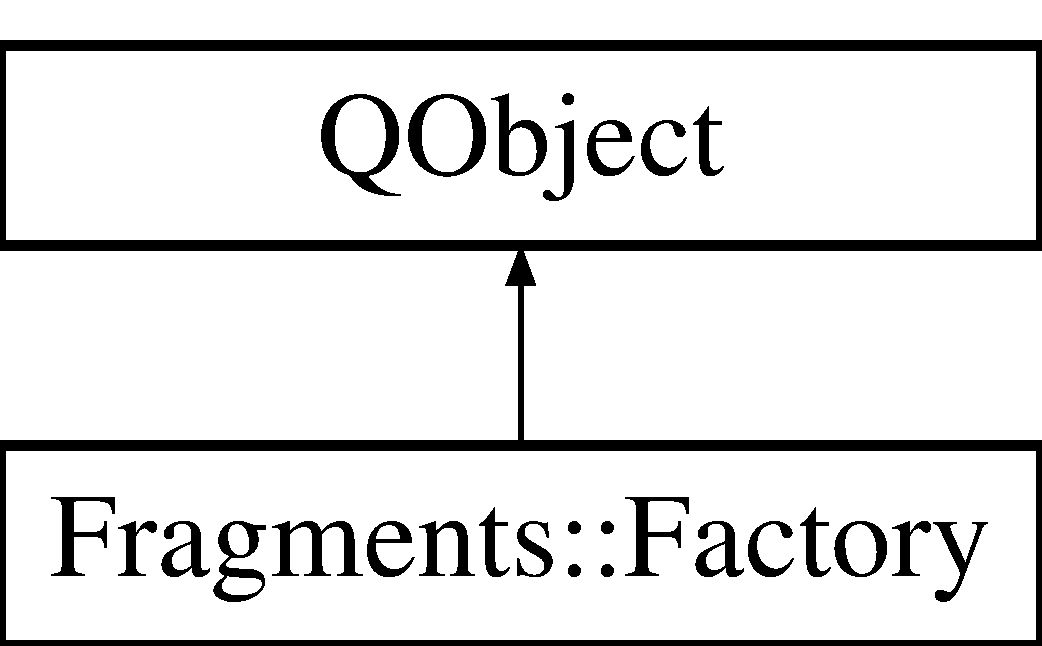
\includegraphics[height=2.000000cm]{classFragments_1_1Factory}
\end{center}
\end{figure}
\subsection*{Signals}
\begin{DoxyCompactItemize}
\item 
void \mbox{\hyperlink{classFragments_1_1Factory_a9559b78a9960c0d4981bf752b47d710a}{page\+Ready}} (\mbox{\hyperlink{classFragments_1_1Page}{Fragments\+::\+Page}} $\ast$page)
\item 
void \mbox{\hyperlink{classFragments_1_1Factory_ac65f072a6cc48bb340e89a61c30688d6}{get\+Resource}} (const Q\+Url \&uri)
\item 
void \mbox{\hyperlink{classFragments_1_1Factory_ab8bdc67290ccbc5444d551fbebc68b17}{error}} (const Q\+String \&message)
\end{DoxyCompactItemize}
\subsection*{Public Member Functions}
\begin{DoxyCompactItemize}
\item 
void \mbox{\hyperlink{classFragments_1_1Factory_a37e59ac23a1a4889a5ef9348f1dfd0bc}{get\+Page}} (const Q\+Url \&uri)
\item 
void \mbox{\hyperlink{classFragments_1_1Factory_a3c9b46f2158e91190305b25616a4bc34}{get\+Page}} (const Q\+Date\+Time \&departure\+Time)
\end{DoxyCompactItemize}
\subsection*{Static Public Member Functions}
\begin{DoxyCompactItemize}
\item 
static \mbox{\hyperlink{classFragments_1_1Factory}{Fragments\+::\+Factory}} $\ast$ \mbox{\hyperlink{classFragments_1_1Factory_a32614388e70b2737a28c045ebbe58e55}{get\+Instance}} (Q\+Object $\ast$parent=nullptr)
\end{DoxyCompactItemize}
\subsection*{Private Slots}
\begin{DoxyCompactItemize}
\item 
void \mbox{\hyperlink{classFragments_1_1Factory_a0ee4ef4c4521a4bce9fe901236a14c84}{process\+H\+T\+T\+P\+Reply}} (Q\+Network\+Reply $\ast$reply)
\end{DoxyCompactItemize}
\subsection*{Private Member Functions}
\begin{DoxyCompactItemize}
\item 
void \mbox{\hyperlink{classFragments_1_1Factory_a9a5923caf97c4e8dba24e23539328deb}{get\+Page\+By\+U\+R\+I\+From\+Network\+Manager}} (const Q\+Url \&uri)
\item 
\mbox{\hyperlink{classFragments_1_1Fragment}{Fragments\+::\+Fragment}} $\ast$ \mbox{\hyperlink{classFragments_1_1Factory_a8f78a634fbeec2b7edb731d778947e97}{generate\+Fragment\+From\+J\+S\+ON}} (const Q\+Json\+Object \&connection)
\item 
bool \mbox{\hyperlink{classFragments_1_1Factory_a62a60fd81fec95b794a8b27188b51824}{validate\+Data}} (const Q\+Json\+Object \&data, const Q\+String\+List \&properties)
\item 
\mbox{\hyperlink{classFragments_1_1Factory_a04aefdf80a3318302fbb839b9322a12e}{Factory}} (Q\+Object $\ast$parent)
\item 
\mbox{\hyperlink{classNetwork_1_1Manager}{Network\+::\+Manager}} $\ast$ \mbox{\hyperlink{classFragments_1_1Factory_ae9f54ac342a7fd5010689d80ef343424}{http}} () const
\item 
void \mbox{\hyperlink{classFragments_1_1Factory_ae5738a3e881b1791dda120e34be3cea9}{set\+Http}} (\mbox{\hyperlink{classNetwork_1_1Manager}{Network\+::\+Manager}} $\ast$\mbox{\hyperlink{classFragments_1_1Factory_ae9f54ac342a7fd5010689d80ef343424}{http}})
\end{DoxyCompactItemize}
\subsection*{Private Attributes}
\begin{DoxyCompactItemize}
\item 
\mbox{\hyperlink{classNetwork_1_1Manager}{Network\+::\+Manager}} $\ast$ \mbox{\hyperlink{classFragments_1_1Factory_aa98b2097fdc55511bdf4fc3bda37e98e}{m\+\_\+http}}
\end{DoxyCompactItemize}
\subsection*{Static Private Attributes}
\begin{DoxyCompactItemize}
\item 
static \mbox{\hyperlink{classFragments_1_1Factory}{Fragments\+::\+Factory}} $\ast$ \mbox{\hyperlink{classFragments_1_1Factory_a7e07aaa093813ab0e1cb50e92ac1386e}{m\+\_\+instance}} = nullptr
\end{DoxyCompactItemize}


\subsection{Constructor \& Destructor Documentation}
\mbox{\Hypertarget{classFragments_1_1Factory_a04aefdf80a3318302fbb839b9322a12e}\label{classFragments_1_1Factory_a04aefdf80a3318302fbb839b9322a12e}} 
\index{Fragments\+::\+Factory@{Fragments\+::\+Factory}!Factory@{Factory}}
\index{Factory@{Factory}!Fragments\+::\+Factory@{Fragments\+::\+Factory}}
\subsubsection{\texorpdfstring{Factory()}{Factory()}}
{\footnotesize\ttfamily Fragments\+::\+Factory\+::\+Factory (\begin{DoxyParamCaption}\item[{Q\+Object $\ast$}]{parent }\end{DoxyParamCaption})\hspace{0.3cm}{\ttfamily [explicit]}, {\ttfamily [private]}}



\subsection{Member Function Documentation}
\mbox{\Hypertarget{classFragments_1_1Factory_ab8bdc67290ccbc5444d551fbebc68b17}\label{classFragments_1_1Factory_ab8bdc67290ccbc5444d551fbebc68b17}} 
\index{Fragments\+::\+Factory@{Fragments\+::\+Factory}!error@{error}}
\index{error@{error}!Fragments\+::\+Factory@{Fragments\+::\+Factory}}
\subsubsection{\texorpdfstring{error}{error}}
{\footnotesize\ttfamily void Fragments\+::\+Factory\+::error (\begin{DoxyParamCaption}\item[{const Q\+String \&}]{message }\end{DoxyParamCaption})\hspace{0.3cm}{\ttfamily [signal]}}

\mbox{\Hypertarget{classFragments_1_1Factory_a8f78a634fbeec2b7edb731d778947e97}\label{classFragments_1_1Factory_a8f78a634fbeec2b7edb731d778947e97}} 
\index{Fragments\+::\+Factory@{Fragments\+::\+Factory}!generate\+Fragment\+From\+J\+S\+ON@{generate\+Fragment\+From\+J\+S\+ON}}
\index{generate\+Fragment\+From\+J\+S\+ON@{generate\+Fragment\+From\+J\+S\+ON}!Fragments\+::\+Factory@{Fragments\+::\+Factory}}
\subsubsection{\texorpdfstring{generate\+Fragment\+From\+J\+S\+O\+N()}{generateFragmentFromJSON()}}
{\footnotesize\ttfamily \mbox{\hyperlink{classFragments_1_1Fragment}{Fragments\+::\+Fragment}} $\ast$ Fragments\+::\+Factory\+::generate\+Fragment\+From\+J\+S\+ON (\begin{DoxyParamCaption}\item[{const Q\+Json\+Object \&}]{connection }\end{DoxyParamCaption})\hspace{0.3cm}{\ttfamily [private]}}

\mbox{\Hypertarget{classFragments_1_1Factory_a32614388e70b2737a28c045ebbe58e55}\label{classFragments_1_1Factory_a32614388e70b2737a28c045ebbe58e55}} 
\index{Fragments\+::\+Factory@{Fragments\+::\+Factory}!get\+Instance@{get\+Instance}}
\index{get\+Instance@{get\+Instance}!Fragments\+::\+Factory@{Fragments\+::\+Factory}}
\subsubsection{\texorpdfstring{get\+Instance()}{getInstance()}}
{\footnotesize\ttfamily \mbox{\hyperlink{classFragments_1_1Factory}{Fragments\+::\+Factory}} $\ast$ Fragments\+::\+Factory\+::get\+Instance (\begin{DoxyParamCaption}\item[{Q\+Object $\ast$}]{parent = {\ttfamily nullptr} }\end{DoxyParamCaption})\hspace{0.3cm}{\ttfamily [static]}}

\mbox{\Hypertarget{classFragments_1_1Factory_a37e59ac23a1a4889a5ef9348f1dfd0bc}\label{classFragments_1_1Factory_a37e59ac23a1a4889a5ef9348f1dfd0bc}} 
\index{Fragments\+::\+Factory@{Fragments\+::\+Factory}!get\+Page@{get\+Page}}
\index{get\+Page@{get\+Page}!Fragments\+::\+Factory@{Fragments\+::\+Factory}}
\subsubsection{\texorpdfstring{get\+Page()}{getPage()}\hspace{0.1cm}{\footnotesize\ttfamily [1/2]}}
{\footnotesize\ttfamily void Fragments\+::\+Factory\+::get\+Page (\begin{DoxyParamCaption}\item[{const Q\+Url \&}]{uri }\end{DoxyParamCaption})}

\mbox{\Hypertarget{classFragments_1_1Factory_a3c9b46f2158e91190305b25616a4bc34}\label{classFragments_1_1Factory_a3c9b46f2158e91190305b25616a4bc34}} 
\index{Fragments\+::\+Factory@{Fragments\+::\+Factory}!get\+Page@{get\+Page}}
\index{get\+Page@{get\+Page}!Fragments\+::\+Factory@{Fragments\+::\+Factory}}
\subsubsection{\texorpdfstring{get\+Page()}{getPage()}\hspace{0.1cm}{\footnotesize\ttfamily [2/2]}}
{\footnotesize\ttfamily void Fragments\+::\+Factory\+::get\+Page (\begin{DoxyParamCaption}\item[{const Q\+Date\+Time \&}]{departure\+Time }\end{DoxyParamCaption})}

\mbox{\Hypertarget{classFragments_1_1Factory_a9a5923caf97c4e8dba24e23539328deb}\label{classFragments_1_1Factory_a9a5923caf97c4e8dba24e23539328deb}} 
\index{Fragments\+::\+Factory@{Fragments\+::\+Factory}!get\+Page\+By\+U\+R\+I\+From\+Network\+Manager@{get\+Page\+By\+U\+R\+I\+From\+Network\+Manager}}
\index{get\+Page\+By\+U\+R\+I\+From\+Network\+Manager@{get\+Page\+By\+U\+R\+I\+From\+Network\+Manager}!Fragments\+::\+Factory@{Fragments\+::\+Factory}}
\subsubsection{\texorpdfstring{get\+Page\+By\+U\+R\+I\+From\+Network\+Manager()}{getPageByURIFromNetworkManager()}}
{\footnotesize\ttfamily void Fragments\+::\+Factory\+::get\+Page\+By\+U\+R\+I\+From\+Network\+Manager (\begin{DoxyParamCaption}\item[{const Q\+Url \&}]{uri }\end{DoxyParamCaption})\hspace{0.3cm}{\ttfamily [private]}}

\mbox{\Hypertarget{classFragments_1_1Factory_ac65f072a6cc48bb340e89a61c30688d6}\label{classFragments_1_1Factory_ac65f072a6cc48bb340e89a61c30688d6}} 
\index{Fragments\+::\+Factory@{Fragments\+::\+Factory}!get\+Resource@{get\+Resource}}
\index{get\+Resource@{get\+Resource}!Fragments\+::\+Factory@{Fragments\+::\+Factory}}
\subsubsection{\texorpdfstring{get\+Resource}{getResource}}
{\footnotesize\ttfamily void Fragments\+::\+Factory\+::get\+Resource (\begin{DoxyParamCaption}\item[{const Q\+Url \&}]{uri }\end{DoxyParamCaption})\hspace{0.3cm}{\ttfamily [signal]}}

\mbox{\Hypertarget{classFragments_1_1Factory_ae9f54ac342a7fd5010689d80ef343424}\label{classFragments_1_1Factory_ae9f54ac342a7fd5010689d80ef343424}} 
\index{Fragments\+::\+Factory@{Fragments\+::\+Factory}!http@{http}}
\index{http@{http}!Fragments\+::\+Factory@{Fragments\+::\+Factory}}
\subsubsection{\texorpdfstring{http()}{http()}}
{\footnotesize\ttfamily \mbox{\hyperlink{classNetwork_1_1Manager}{Network\+::\+Manager}} $\ast$ Fragments\+::\+Factory\+::http (\begin{DoxyParamCaption}{ }\end{DoxyParamCaption}) const\hspace{0.3cm}{\ttfamily [private]}}

\mbox{\Hypertarget{classFragments_1_1Factory_a9559b78a9960c0d4981bf752b47d710a}\label{classFragments_1_1Factory_a9559b78a9960c0d4981bf752b47d710a}} 
\index{Fragments\+::\+Factory@{Fragments\+::\+Factory}!page\+Ready@{page\+Ready}}
\index{page\+Ready@{page\+Ready}!Fragments\+::\+Factory@{Fragments\+::\+Factory}}
\subsubsection{\texorpdfstring{page\+Ready}{pageReady}}
{\footnotesize\ttfamily void Fragments\+::\+Factory\+::page\+Ready (\begin{DoxyParamCaption}\item[{\mbox{\hyperlink{classFragments_1_1Page}{Fragments\+::\+Page}} $\ast$}]{page }\end{DoxyParamCaption})\hspace{0.3cm}{\ttfamily [signal]}}

\mbox{\Hypertarget{classFragments_1_1Factory_a0ee4ef4c4521a4bce9fe901236a14c84}\label{classFragments_1_1Factory_a0ee4ef4c4521a4bce9fe901236a14c84}} 
\index{Fragments\+::\+Factory@{Fragments\+::\+Factory}!process\+H\+T\+T\+P\+Reply@{process\+H\+T\+T\+P\+Reply}}
\index{process\+H\+T\+T\+P\+Reply@{process\+H\+T\+T\+P\+Reply}!Fragments\+::\+Factory@{Fragments\+::\+Factory}}
\subsubsection{\texorpdfstring{process\+H\+T\+T\+P\+Reply}{processHTTPReply}}
{\footnotesize\ttfamily void Fragments\+::\+Factory\+::process\+H\+T\+T\+P\+Reply (\begin{DoxyParamCaption}\item[{Q\+Network\+Reply $\ast$}]{reply }\end{DoxyParamCaption})\hspace{0.3cm}{\ttfamily [private]}, {\ttfamily [slot]}}

\mbox{\Hypertarget{classFragments_1_1Factory_ae5738a3e881b1791dda120e34be3cea9}\label{classFragments_1_1Factory_ae5738a3e881b1791dda120e34be3cea9}} 
\index{Fragments\+::\+Factory@{Fragments\+::\+Factory}!set\+Http@{set\+Http}}
\index{set\+Http@{set\+Http}!Fragments\+::\+Factory@{Fragments\+::\+Factory}}
\subsubsection{\texorpdfstring{set\+Http()}{setHttp()}}
{\footnotesize\ttfamily void Fragments\+::\+Factory\+::set\+Http (\begin{DoxyParamCaption}\item[{\mbox{\hyperlink{classNetwork_1_1Manager}{Network\+::\+Manager}} $\ast$}]{http }\end{DoxyParamCaption})\hspace{0.3cm}{\ttfamily [private]}}

\mbox{\Hypertarget{classFragments_1_1Factory_a62a60fd81fec95b794a8b27188b51824}\label{classFragments_1_1Factory_a62a60fd81fec95b794a8b27188b51824}} 
\index{Fragments\+::\+Factory@{Fragments\+::\+Factory}!validate\+Data@{validate\+Data}}
\index{validate\+Data@{validate\+Data}!Fragments\+::\+Factory@{Fragments\+::\+Factory}}
\subsubsection{\texorpdfstring{validate\+Data()}{validateData()}}
{\footnotesize\ttfamily bool Fragments\+::\+Factory\+::validate\+Data (\begin{DoxyParamCaption}\item[{const Q\+Json\+Object \&}]{data,  }\item[{const Q\+String\+List \&}]{properties }\end{DoxyParamCaption})\hspace{0.3cm}{\ttfamily [private]}}



\subsection{Member Data Documentation}
\mbox{\Hypertarget{classFragments_1_1Factory_aa98b2097fdc55511bdf4fc3bda37e98e}\label{classFragments_1_1Factory_aa98b2097fdc55511bdf4fc3bda37e98e}} 
\index{Fragments\+::\+Factory@{Fragments\+::\+Factory}!m\+\_\+http@{m\+\_\+http}}
\index{m\+\_\+http@{m\+\_\+http}!Fragments\+::\+Factory@{Fragments\+::\+Factory}}
\subsubsection{\texorpdfstring{m\+\_\+http}{m\_http}}
{\footnotesize\ttfamily \mbox{\hyperlink{classNetwork_1_1Manager}{Network\+::\+Manager}}$\ast$ Fragments\+::\+Factory\+::m\+\_\+http\hspace{0.3cm}{\ttfamily [private]}}

\mbox{\Hypertarget{classFragments_1_1Factory_a7e07aaa093813ab0e1cb50e92ac1386e}\label{classFragments_1_1Factory_a7e07aaa093813ab0e1cb50e92ac1386e}} 
\index{Fragments\+::\+Factory@{Fragments\+::\+Factory}!m\+\_\+instance@{m\+\_\+instance}}
\index{m\+\_\+instance@{m\+\_\+instance}!Fragments\+::\+Factory@{Fragments\+::\+Factory}}
\subsubsection{\texorpdfstring{m\+\_\+instance}{m\_instance}}
{\footnotesize\ttfamily \mbox{\hyperlink{classFragments_1_1Factory}{Fragments\+::\+Factory}} $\ast$ Fragments\+::\+Factory\+::m\+\_\+instance = nullptr\hspace{0.3cm}{\ttfamily [static]}, {\ttfamily [private]}}



The documentation for this class was generated from the following files\+:\begin{DoxyCompactItemize}
\item 
src/linkedconnections/fragments/\mbox{\hyperlink{fragmentsfactory_8h}{fragmentsfactory.\+h}}\item 
src/linkedconnections/fragments/\mbox{\hyperlink{fragmentsfactory_8cpp}{fragmentsfactory.\+cpp}}\end{DoxyCompactItemize}

\hypertarget{classFragments_1_1Fragment}{}\section{Fragments\+:\+:Fragment Class Reference}
\label{classFragments_1_1Fragment}\index{Fragments\+::\+Fragment@{Fragments\+::\+Fragment}}


{\ttfamily \#include $<$fragmentsfragment.\+h$>$}

Inheritance diagram for Fragments\+:\+:Fragment\+:\begin{figure}[H]
\begin{center}
\leavevmode
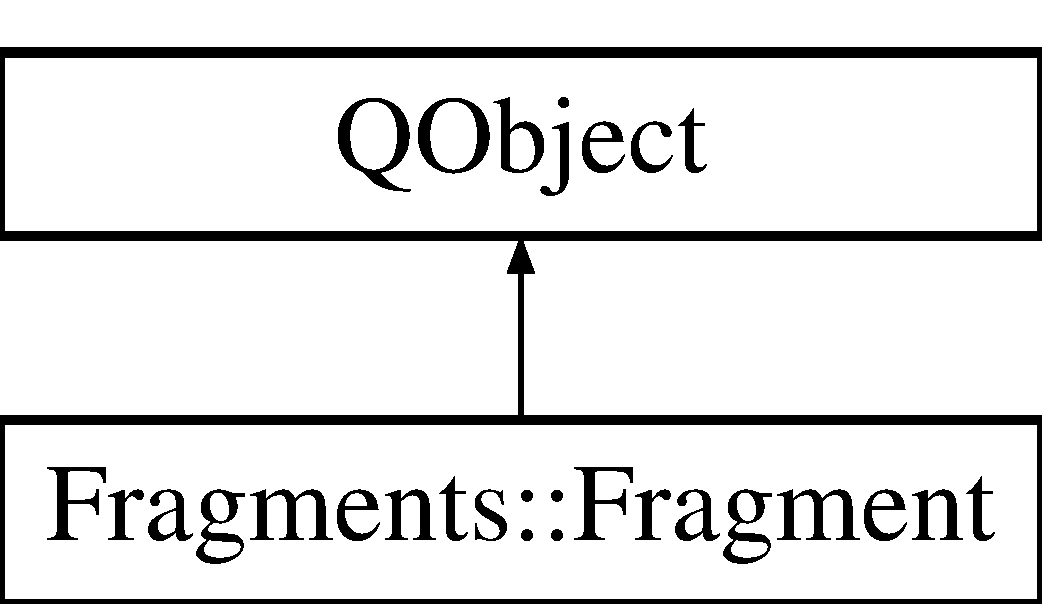
\includegraphics[height=2.000000cm]{classFragments_1_1Fragment}
\end{center}
\end{figure}
\subsection*{Signals}
\begin{DoxyCompactItemize}
\item 
void \mbox{\hyperlink{classFragments_1_1Fragment_ad1d14027cf24dea3982576f160ed61e4}{uri\+Changed}} ()
\item 
void \mbox{\hyperlink{classFragments_1_1Fragment_add02014358cc604a4d5473ff317b9048}{departure\+Station\+U\+R\+I\+Changed}} ()
\item 
void \mbox{\hyperlink{classFragments_1_1Fragment_ab3afd2b0cd0d1fe7a0dc15cd7c358195}{arrival\+Station\+U\+R\+I\+Changed}} ()
\item 
void \mbox{\hyperlink{classFragments_1_1Fragment_a3b4eaf02e54dcf202c5b740c6e3946e6}{departure\+Time\+Changed}} ()
\item 
void \mbox{\hyperlink{classFragments_1_1Fragment_a25530427fe0bc865f7595221a8284ef2}{arrival\+Time\+Changed}} ()
\item 
void \mbox{\hyperlink{classFragments_1_1Fragment_a2f4407d54a869e2a45b514525c582016}{departure\+Delay\+Changed}} ()
\item 
void \mbox{\hyperlink{classFragments_1_1Fragment_a586fd07ea637247637da6971555ed92b}{arrival\+Delay\+Changed}} ()
\item 
void \mbox{\hyperlink{classFragments_1_1Fragment_a80a2dcba09a29a4d375b8900bb6b6be0}{trip\+U\+R\+I\+Changed}} ()
\item 
void \mbox{\hyperlink{classFragments_1_1Fragment_ab220e9fef71bf161e14769afc61f0499}{route\+U\+R\+I\+Changed}} ()
\item 
void \mbox{\hyperlink{classFragments_1_1Fragment_a5956fb561df3842d6d292b46fc16bec2}{direction\+Changed}} ()
\end{DoxyCompactItemize}
\subsection*{Public Member Functions}
\begin{DoxyCompactItemize}
\item 
\mbox{\hyperlink{classFragments_1_1Fragment_a08e16b988d340a5e836c377a13e1c41d}{Fragment}} (Q\+Object $\ast$parent=nullptr)
\item 
\mbox{\hyperlink{classFragments_1_1Fragment_a26ec3793c4162b77e92498a77ae5b7dc}{Fragment}} (const Q\+Url \&\mbox{\hyperlink{classFragments_1_1Fragment_a8123bbbb75221107730898627b99ffec}{uri}}, const Q\+Url \&\mbox{\hyperlink{classFragments_1_1Fragment_aaca4de063cdd1df3f130ade1a0df8dfa}{departure\+Station\+U\+RI}}, const Q\+Url \&\mbox{\hyperlink{classFragments_1_1Fragment_a74d2fae0d687f2389121fb720f8f6505}{arrival\+Station\+U\+RI}}, const Q\+Date\+Time \&\mbox{\hyperlink{classFragments_1_1Fragment_adfcf2bb9a548f41f4ca88ad117c655a3}{departure\+Time}}, const Q\+Date\+Time \&\mbox{\hyperlink{classFragments_1_1Fragment_aa7e96d4d8b9e36c19d3f6134ff3072e9}{arrival\+Time}}, const qint16 \&\mbox{\hyperlink{classFragments_1_1Fragment_a8c8363f22d1aca339a66d342f9e5f0c8}{departure\+Delay}}, const qint16 \&\mbox{\hyperlink{classFragments_1_1Fragment_aec60f571141b0c7aacbc172e83a4a2d3}{arrival\+Delay}}, const Q\+Url \&\mbox{\hyperlink{classFragments_1_1Fragment_aa3b1beb97e501bfa8ecb2127c2729803}{trip\+U\+RI}}, const Q\+Url \&\mbox{\hyperlink{classFragments_1_1Fragment_a58ca3c71db8995b1a60b1eee17d65911}{route\+U\+RI}}, const Q\+String \&\mbox{\hyperlink{classFragments_1_1Fragment_a1c0ff28939d612a28589fdc1f47d0fd5}{direction}}, Q\+Object $\ast$parent=nullptr)
\item 
Q\+Url \mbox{\hyperlink{classFragments_1_1Fragment_a8123bbbb75221107730898627b99ffec}{uri}} () const
\item 
void \mbox{\hyperlink{classFragments_1_1Fragment_ab4ad3107834caa289cfbed904f052fc0}{set\+U\+RI}} (const Q\+Url \&\mbox{\hyperlink{classFragments_1_1Fragment_a8123bbbb75221107730898627b99ffec}{uri}})
\item 
Q\+Url \mbox{\hyperlink{classFragments_1_1Fragment_aaca4de063cdd1df3f130ade1a0df8dfa}{departure\+Station\+U\+RI}} () const
\item 
void \mbox{\hyperlink{classFragments_1_1Fragment_a8c9ffce21e97be8e50e2ca1654da507f}{set\+Departure\+Station\+U\+RI}} (const Q\+Url \&\mbox{\hyperlink{classFragments_1_1Fragment_aaca4de063cdd1df3f130ade1a0df8dfa}{departure\+Station\+U\+RI}})
\item 
Q\+Url \mbox{\hyperlink{classFragments_1_1Fragment_a74d2fae0d687f2389121fb720f8f6505}{arrival\+Station\+U\+RI}} () const
\item 
void \mbox{\hyperlink{classFragments_1_1Fragment_af18c29375ad402d4ec02133fb5534a8e}{set\+Arrival\+Station\+U\+RI}} (const Q\+Url \&\mbox{\hyperlink{classFragments_1_1Fragment_a74d2fae0d687f2389121fb720f8f6505}{arrival\+Station\+U\+RI}})
\item 
Q\+Date\+Time \mbox{\hyperlink{classFragments_1_1Fragment_adfcf2bb9a548f41f4ca88ad117c655a3}{departure\+Time}} () const
\item 
void \mbox{\hyperlink{classFragments_1_1Fragment_a595b2c52c5cbaab0a97ceda63028d91d}{set\+Departure\+Time}} (const Q\+Date\+Time \&\mbox{\hyperlink{classFragments_1_1Fragment_adfcf2bb9a548f41f4ca88ad117c655a3}{departure\+Time}})
\item 
Q\+Date\+Time \mbox{\hyperlink{classFragments_1_1Fragment_aa7e96d4d8b9e36c19d3f6134ff3072e9}{arrival\+Time}} () const
\item 
void \mbox{\hyperlink{classFragments_1_1Fragment_a5b7ed13c7d4417f3b4f3d87aebd68a90}{set\+Arrival\+Time}} (const Q\+Date\+Time \&\mbox{\hyperlink{classFragments_1_1Fragment_aa7e96d4d8b9e36c19d3f6134ff3072e9}{arrival\+Time}})
\item 
qint16 \mbox{\hyperlink{classFragments_1_1Fragment_a8c8363f22d1aca339a66d342f9e5f0c8}{departure\+Delay}} () const
\item 
void \mbox{\hyperlink{classFragments_1_1Fragment_a3293b86baeee32223a5019594fb1ae82}{set\+Departure\+Delay}} (const qint16 \&\mbox{\hyperlink{classFragments_1_1Fragment_a8c8363f22d1aca339a66d342f9e5f0c8}{departure\+Delay}})
\item 
qint16 \mbox{\hyperlink{classFragments_1_1Fragment_aec60f571141b0c7aacbc172e83a4a2d3}{arrival\+Delay}} () const
\item 
void \mbox{\hyperlink{classFragments_1_1Fragment_ae5df59623d6835ec0224d58f9f3903db}{set\+Arrival\+Delay}} (const qint16 \&\mbox{\hyperlink{classFragments_1_1Fragment_aec60f571141b0c7aacbc172e83a4a2d3}{arrival\+Delay}})
\item 
Q\+Date\+Time \mbox{\hyperlink{classFragments_1_1Fragment_a23f4a6f0401e2d2e6aa2f53621beefa0}{departure\+Delayed\+Time}} () const
\item 
Q\+Date\+Time \mbox{\hyperlink{classFragments_1_1Fragment_a9948ab3690d2c290eda2adc89415e2b2}{arrival\+Delayed\+Time}} () const
\item 
Q\+Url \mbox{\hyperlink{classFragments_1_1Fragment_aa3b1beb97e501bfa8ecb2127c2729803}{trip\+U\+RI}} () const
\item 
void \mbox{\hyperlink{classFragments_1_1Fragment_a47c214a918ce0fe7469b309cbecf01a1}{set\+Trip\+U\+RI}} (const Q\+Url \&\mbox{\hyperlink{classFragments_1_1Fragment_aa3b1beb97e501bfa8ecb2127c2729803}{trip\+U\+RI}})
\item 
Q\+Url \mbox{\hyperlink{classFragments_1_1Fragment_a58ca3c71db8995b1a60b1eee17d65911}{route\+U\+RI}} () const
\item 
void \mbox{\hyperlink{classFragments_1_1Fragment_a26880f6f3800e4609685f1316b6db257}{set\+Route\+U\+RI}} (const Q\+Url \&\mbox{\hyperlink{classFragments_1_1Fragment_a58ca3c71db8995b1a60b1eee17d65911}{route\+U\+RI}})
\item 
Q\+String \mbox{\hyperlink{classFragments_1_1Fragment_a1c0ff28939d612a28589fdc1f47d0fd5}{direction}} () const
\item 
void \mbox{\hyperlink{classFragments_1_1Fragment_a0de734da455ac32aad779520d9cc7a10}{set\+Direction}} (const Q\+String \&\mbox{\hyperlink{classFragments_1_1Fragment_a1c0ff28939d612a28589fdc1f47d0fd5}{direction}})
\end{DoxyCompactItemize}
\subsection*{Private Attributes}
\begin{DoxyCompactItemize}
\item 
Q\+Url \mbox{\hyperlink{classFragments_1_1Fragment_a5e60c2e6902a55c1e2a3bb7a97d390f5}{m\+\_\+uri}}
\item 
Q\+Url \mbox{\hyperlink{classFragments_1_1Fragment_ad283a69630de2d45564976d8f4f20494}{m\+\_\+departure\+Station\+U\+RI}}
\item 
Q\+Url \mbox{\hyperlink{classFragments_1_1Fragment_ae7965d7528238e79ad22fd5f07666913}{m\+\_\+arrival\+Station\+U\+RI}}
\item 
Q\+Date\+Time \mbox{\hyperlink{classFragments_1_1Fragment_a0e8fdc91c05e8770524e5069e63a1c8d}{m\+\_\+departure\+Time}}
\item 
Q\+Date\+Time \mbox{\hyperlink{classFragments_1_1Fragment_ae9a5e9389dbe68090f9b14a73cf6ec32}{m\+\_\+arrival\+Time}}
\item 
qint16 \mbox{\hyperlink{classFragments_1_1Fragment_a4191e1af11c31f3b6e87ec860e2a51e1}{m\+\_\+departure\+Delay}}
\item 
qint16 \mbox{\hyperlink{classFragments_1_1Fragment_ab73eb5dd910919a3b74da379489ab51e}{m\+\_\+arrival\+Delay}}
\item 
Q\+Url \mbox{\hyperlink{classFragments_1_1Fragment_abd0750b77264363fe0069764fd7aeb3c}{m\+\_\+trip\+U\+RI}}
\item 
Q\+Url \mbox{\hyperlink{classFragments_1_1Fragment_a7540fc6c97499e59d7bc582bfc142dbb}{m\+\_\+route\+U\+RI}}
\item 
Q\+String \mbox{\hyperlink{classFragments_1_1Fragment_acc9b5abffc1a65636063e42943a9e529}{m\+\_\+direction}}
\end{DoxyCompactItemize}


\subsection{Constructor \& Destructor Documentation}
\mbox{\Hypertarget{classFragments_1_1Fragment_a08e16b988d340a5e836c377a13e1c41d}\label{classFragments_1_1Fragment_a08e16b988d340a5e836c377a13e1c41d}} 
\index{Fragments\+::\+Fragment@{Fragments\+::\+Fragment}!Fragment@{Fragment}}
\index{Fragment@{Fragment}!Fragments\+::\+Fragment@{Fragments\+::\+Fragment}}
\subsubsection{\texorpdfstring{Fragment()}{Fragment()}\hspace{0.1cm}{\footnotesize\ttfamily [1/2]}}
{\footnotesize\ttfamily Fragments\+::\+Fragment\+::\+Fragment (\begin{DoxyParamCaption}\item[{Q\+Object $\ast$}]{parent = {\ttfamily nullptr} }\end{DoxyParamCaption})\hspace{0.3cm}{\ttfamily [explicit]}}

\mbox{\Hypertarget{classFragments_1_1Fragment_a26ec3793c4162b77e92498a77ae5b7dc}\label{classFragments_1_1Fragment_a26ec3793c4162b77e92498a77ae5b7dc}} 
\index{Fragments\+::\+Fragment@{Fragments\+::\+Fragment}!Fragment@{Fragment}}
\index{Fragment@{Fragment}!Fragments\+::\+Fragment@{Fragments\+::\+Fragment}}
\subsubsection{\texorpdfstring{Fragment()}{Fragment()}\hspace{0.1cm}{\footnotesize\ttfamily [2/2]}}
{\footnotesize\ttfamily Fragments\+::\+Fragment\+::\+Fragment (\begin{DoxyParamCaption}\item[{const Q\+Url \&}]{uri,  }\item[{const Q\+Url \&}]{departure\+Station\+U\+RI,  }\item[{const Q\+Url \&}]{arrival\+Station\+U\+RI,  }\item[{const Q\+Date\+Time \&}]{departure\+Time,  }\item[{const Q\+Date\+Time \&}]{arrival\+Time,  }\item[{const qint16 \&}]{departure\+Delay,  }\item[{const qint16 \&}]{arrival\+Delay,  }\item[{const Q\+Url \&}]{trip\+U\+RI,  }\item[{const Q\+Url \&}]{route\+U\+RI,  }\item[{const Q\+String \&}]{direction,  }\item[{Q\+Object $\ast$}]{parent = {\ttfamily nullptr} }\end{DoxyParamCaption})\hspace{0.3cm}{\ttfamily [explicit]}}



\subsection{Member Function Documentation}
\mbox{\Hypertarget{classFragments_1_1Fragment_aec60f571141b0c7aacbc172e83a4a2d3}\label{classFragments_1_1Fragment_aec60f571141b0c7aacbc172e83a4a2d3}} 
\index{Fragments\+::\+Fragment@{Fragments\+::\+Fragment}!arrival\+Delay@{arrival\+Delay}}
\index{arrival\+Delay@{arrival\+Delay}!Fragments\+::\+Fragment@{Fragments\+::\+Fragment}}
\subsubsection{\texorpdfstring{arrival\+Delay()}{arrivalDelay()}}
{\footnotesize\ttfamily qint16 Fragments\+::\+Fragment\+::arrival\+Delay (\begin{DoxyParamCaption}{ }\end{DoxyParamCaption}) const}

\mbox{\Hypertarget{classFragments_1_1Fragment_a586fd07ea637247637da6971555ed92b}\label{classFragments_1_1Fragment_a586fd07ea637247637da6971555ed92b}} 
\index{Fragments\+::\+Fragment@{Fragments\+::\+Fragment}!arrival\+Delay\+Changed@{arrival\+Delay\+Changed}}
\index{arrival\+Delay\+Changed@{arrival\+Delay\+Changed}!Fragments\+::\+Fragment@{Fragments\+::\+Fragment}}
\subsubsection{\texorpdfstring{arrival\+Delay\+Changed}{arrivalDelayChanged}}
{\footnotesize\ttfamily void Fragments\+::\+Fragment\+::arrival\+Delay\+Changed (\begin{DoxyParamCaption}{ }\end{DoxyParamCaption})\hspace{0.3cm}{\ttfamily [signal]}}

\mbox{\Hypertarget{classFragments_1_1Fragment_a9948ab3690d2c290eda2adc89415e2b2}\label{classFragments_1_1Fragment_a9948ab3690d2c290eda2adc89415e2b2}} 
\index{Fragments\+::\+Fragment@{Fragments\+::\+Fragment}!arrival\+Delayed\+Time@{arrival\+Delayed\+Time}}
\index{arrival\+Delayed\+Time@{arrival\+Delayed\+Time}!Fragments\+::\+Fragment@{Fragments\+::\+Fragment}}
\subsubsection{\texorpdfstring{arrival\+Delayed\+Time()}{arrivalDelayedTime()}}
{\footnotesize\ttfamily Q\+Date\+Time Fragments\+::\+Fragment\+::arrival\+Delayed\+Time (\begin{DoxyParamCaption}{ }\end{DoxyParamCaption}) const}

\mbox{\Hypertarget{classFragments_1_1Fragment_a74d2fae0d687f2389121fb720f8f6505}\label{classFragments_1_1Fragment_a74d2fae0d687f2389121fb720f8f6505}} 
\index{Fragments\+::\+Fragment@{Fragments\+::\+Fragment}!arrival\+Station\+U\+RI@{arrival\+Station\+U\+RI}}
\index{arrival\+Station\+U\+RI@{arrival\+Station\+U\+RI}!Fragments\+::\+Fragment@{Fragments\+::\+Fragment}}
\subsubsection{\texorpdfstring{arrival\+Station\+U\+R\+I()}{arrivalStationURI()}}
{\footnotesize\ttfamily Q\+Url Fragments\+::\+Fragment\+::arrival\+Station\+U\+RI (\begin{DoxyParamCaption}{ }\end{DoxyParamCaption}) const}

\mbox{\Hypertarget{classFragments_1_1Fragment_ab3afd2b0cd0d1fe7a0dc15cd7c358195}\label{classFragments_1_1Fragment_ab3afd2b0cd0d1fe7a0dc15cd7c358195}} 
\index{Fragments\+::\+Fragment@{Fragments\+::\+Fragment}!arrival\+Station\+U\+R\+I\+Changed@{arrival\+Station\+U\+R\+I\+Changed}}
\index{arrival\+Station\+U\+R\+I\+Changed@{arrival\+Station\+U\+R\+I\+Changed}!Fragments\+::\+Fragment@{Fragments\+::\+Fragment}}
\subsubsection{\texorpdfstring{arrival\+Station\+U\+R\+I\+Changed}{arrivalStationURIChanged}}
{\footnotesize\ttfamily void Fragments\+::\+Fragment\+::arrival\+Station\+U\+R\+I\+Changed (\begin{DoxyParamCaption}{ }\end{DoxyParamCaption})\hspace{0.3cm}{\ttfamily [signal]}}

\mbox{\Hypertarget{classFragments_1_1Fragment_aa7e96d4d8b9e36c19d3f6134ff3072e9}\label{classFragments_1_1Fragment_aa7e96d4d8b9e36c19d3f6134ff3072e9}} 
\index{Fragments\+::\+Fragment@{Fragments\+::\+Fragment}!arrival\+Time@{arrival\+Time}}
\index{arrival\+Time@{arrival\+Time}!Fragments\+::\+Fragment@{Fragments\+::\+Fragment}}
\subsubsection{\texorpdfstring{arrival\+Time()}{arrivalTime()}}
{\footnotesize\ttfamily Q\+Date\+Time Fragments\+::\+Fragment\+::arrival\+Time (\begin{DoxyParamCaption}{ }\end{DoxyParamCaption}) const}

\mbox{\Hypertarget{classFragments_1_1Fragment_a25530427fe0bc865f7595221a8284ef2}\label{classFragments_1_1Fragment_a25530427fe0bc865f7595221a8284ef2}} 
\index{Fragments\+::\+Fragment@{Fragments\+::\+Fragment}!arrival\+Time\+Changed@{arrival\+Time\+Changed}}
\index{arrival\+Time\+Changed@{arrival\+Time\+Changed}!Fragments\+::\+Fragment@{Fragments\+::\+Fragment}}
\subsubsection{\texorpdfstring{arrival\+Time\+Changed}{arrivalTimeChanged}}
{\footnotesize\ttfamily void Fragments\+::\+Fragment\+::arrival\+Time\+Changed (\begin{DoxyParamCaption}{ }\end{DoxyParamCaption})\hspace{0.3cm}{\ttfamily [signal]}}

\mbox{\Hypertarget{classFragments_1_1Fragment_a8c8363f22d1aca339a66d342f9e5f0c8}\label{classFragments_1_1Fragment_a8c8363f22d1aca339a66d342f9e5f0c8}} 
\index{Fragments\+::\+Fragment@{Fragments\+::\+Fragment}!departure\+Delay@{departure\+Delay}}
\index{departure\+Delay@{departure\+Delay}!Fragments\+::\+Fragment@{Fragments\+::\+Fragment}}
\subsubsection{\texorpdfstring{departure\+Delay()}{departureDelay()}}
{\footnotesize\ttfamily qint16 Fragments\+::\+Fragment\+::departure\+Delay (\begin{DoxyParamCaption}{ }\end{DoxyParamCaption}) const}

\mbox{\Hypertarget{classFragments_1_1Fragment_a2f4407d54a869e2a45b514525c582016}\label{classFragments_1_1Fragment_a2f4407d54a869e2a45b514525c582016}} 
\index{Fragments\+::\+Fragment@{Fragments\+::\+Fragment}!departure\+Delay\+Changed@{departure\+Delay\+Changed}}
\index{departure\+Delay\+Changed@{departure\+Delay\+Changed}!Fragments\+::\+Fragment@{Fragments\+::\+Fragment}}
\subsubsection{\texorpdfstring{departure\+Delay\+Changed}{departureDelayChanged}}
{\footnotesize\ttfamily void Fragments\+::\+Fragment\+::departure\+Delay\+Changed (\begin{DoxyParamCaption}{ }\end{DoxyParamCaption})\hspace{0.3cm}{\ttfamily [signal]}}

\mbox{\Hypertarget{classFragments_1_1Fragment_a23f4a6f0401e2d2e6aa2f53621beefa0}\label{classFragments_1_1Fragment_a23f4a6f0401e2d2e6aa2f53621beefa0}} 
\index{Fragments\+::\+Fragment@{Fragments\+::\+Fragment}!departure\+Delayed\+Time@{departure\+Delayed\+Time}}
\index{departure\+Delayed\+Time@{departure\+Delayed\+Time}!Fragments\+::\+Fragment@{Fragments\+::\+Fragment}}
\subsubsection{\texorpdfstring{departure\+Delayed\+Time()}{departureDelayedTime()}}
{\footnotesize\ttfamily Q\+Date\+Time Fragments\+::\+Fragment\+::departure\+Delayed\+Time (\begin{DoxyParamCaption}{ }\end{DoxyParamCaption}) const}

\mbox{\Hypertarget{classFragments_1_1Fragment_aaca4de063cdd1df3f130ade1a0df8dfa}\label{classFragments_1_1Fragment_aaca4de063cdd1df3f130ade1a0df8dfa}} 
\index{Fragments\+::\+Fragment@{Fragments\+::\+Fragment}!departure\+Station\+U\+RI@{departure\+Station\+U\+RI}}
\index{departure\+Station\+U\+RI@{departure\+Station\+U\+RI}!Fragments\+::\+Fragment@{Fragments\+::\+Fragment}}
\subsubsection{\texorpdfstring{departure\+Station\+U\+R\+I()}{departureStationURI()}}
{\footnotesize\ttfamily Q\+Url Fragments\+::\+Fragment\+::departure\+Station\+U\+RI (\begin{DoxyParamCaption}{ }\end{DoxyParamCaption}) const}

\mbox{\Hypertarget{classFragments_1_1Fragment_add02014358cc604a4d5473ff317b9048}\label{classFragments_1_1Fragment_add02014358cc604a4d5473ff317b9048}} 
\index{Fragments\+::\+Fragment@{Fragments\+::\+Fragment}!departure\+Station\+U\+R\+I\+Changed@{departure\+Station\+U\+R\+I\+Changed}}
\index{departure\+Station\+U\+R\+I\+Changed@{departure\+Station\+U\+R\+I\+Changed}!Fragments\+::\+Fragment@{Fragments\+::\+Fragment}}
\subsubsection{\texorpdfstring{departure\+Station\+U\+R\+I\+Changed}{departureStationURIChanged}}
{\footnotesize\ttfamily void Fragments\+::\+Fragment\+::departure\+Station\+U\+R\+I\+Changed (\begin{DoxyParamCaption}{ }\end{DoxyParamCaption})\hspace{0.3cm}{\ttfamily [signal]}}

\mbox{\Hypertarget{classFragments_1_1Fragment_adfcf2bb9a548f41f4ca88ad117c655a3}\label{classFragments_1_1Fragment_adfcf2bb9a548f41f4ca88ad117c655a3}} 
\index{Fragments\+::\+Fragment@{Fragments\+::\+Fragment}!departure\+Time@{departure\+Time}}
\index{departure\+Time@{departure\+Time}!Fragments\+::\+Fragment@{Fragments\+::\+Fragment}}
\subsubsection{\texorpdfstring{departure\+Time()}{departureTime()}}
{\footnotesize\ttfamily Q\+Date\+Time Fragments\+::\+Fragment\+::departure\+Time (\begin{DoxyParamCaption}{ }\end{DoxyParamCaption}) const}

\mbox{\Hypertarget{classFragments_1_1Fragment_a3b4eaf02e54dcf202c5b740c6e3946e6}\label{classFragments_1_1Fragment_a3b4eaf02e54dcf202c5b740c6e3946e6}} 
\index{Fragments\+::\+Fragment@{Fragments\+::\+Fragment}!departure\+Time\+Changed@{departure\+Time\+Changed}}
\index{departure\+Time\+Changed@{departure\+Time\+Changed}!Fragments\+::\+Fragment@{Fragments\+::\+Fragment}}
\subsubsection{\texorpdfstring{departure\+Time\+Changed}{departureTimeChanged}}
{\footnotesize\ttfamily void Fragments\+::\+Fragment\+::departure\+Time\+Changed (\begin{DoxyParamCaption}{ }\end{DoxyParamCaption})\hspace{0.3cm}{\ttfamily [signal]}}

\mbox{\Hypertarget{classFragments_1_1Fragment_a1c0ff28939d612a28589fdc1f47d0fd5}\label{classFragments_1_1Fragment_a1c0ff28939d612a28589fdc1f47d0fd5}} 
\index{Fragments\+::\+Fragment@{Fragments\+::\+Fragment}!direction@{direction}}
\index{direction@{direction}!Fragments\+::\+Fragment@{Fragments\+::\+Fragment}}
\subsubsection{\texorpdfstring{direction()}{direction()}}
{\footnotesize\ttfamily Q\+String Fragments\+::\+Fragment\+::direction (\begin{DoxyParamCaption}{ }\end{DoxyParamCaption}) const}

\mbox{\Hypertarget{classFragments_1_1Fragment_a5956fb561df3842d6d292b46fc16bec2}\label{classFragments_1_1Fragment_a5956fb561df3842d6d292b46fc16bec2}} 
\index{Fragments\+::\+Fragment@{Fragments\+::\+Fragment}!direction\+Changed@{direction\+Changed}}
\index{direction\+Changed@{direction\+Changed}!Fragments\+::\+Fragment@{Fragments\+::\+Fragment}}
\subsubsection{\texorpdfstring{direction\+Changed}{directionChanged}}
{\footnotesize\ttfamily void Fragments\+::\+Fragment\+::direction\+Changed (\begin{DoxyParamCaption}{ }\end{DoxyParamCaption})\hspace{0.3cm}{\ttfamily [signal]}}

\mbox{\Hypertarget{classFragments_1_1Fragment_a58ca3c71db8995b1a60b1eee17d65911}\label{classFragments_1_1Fragment_a58ca3c71db8995b1a60b1eee17d65911}} 
\index{Fragments\+::\+Fragment@{Fragments\+::\+Fragment}!route\+U\+RI@{route\+U\+RI}}
\index{route\+U\+RI@{route\+U\+RI}!Fragments\+::\+Fragment@{Fragments\+::\+Fragment}}
\subsubsection{\texorpdfstring{route\+U\+R\+I()}{routeURI()}}
{\footnotesize\ttfamily Q\+Url Fragments\+::\+Fragment\+::route\+U\+RI (\begin{DoxyParamCaption}{ }\end{DoxyParamCaption}) const}

\mbox{\Hypertarget{classFragments_1_1Fragment_ab220e9fef71bf161e14769afc61f0499}\label{classFragments_1_1Fragment_ab220e9fef71bf161e14769afc61f0499}} 
\index{Fragments\+::\+Fragment@{Fragments\+::\+Fragment}!route\+U\+R\+I\+Changed@{route\+U\+R\+I\+Changed}}
\index{route\+U\+R\+I\+Changed@{route\+U\+R\+I\+Changed}!Fragments\+::\+Fragment@{Fragments\+::\+Fragment}}
\subsubsection{\texorpdfstring{route\+U\+R\+I\+Changed}{routeURIChanged}}
{\footnotesize\ttfamily void Fragments\+::\+Fragment\+::route\+U\+R\+I\+Changed (\begin{DoxyParamCaption}{ }\end{DoxyParamCaption})\hspace{0.3cm}{\ttfamily [signal]}}

\mbox{\Hypertarget{classFragments_1_1Fragment_ae5df59623d6835ec0224d58f9f3903db}\label{classFragments_1_1Fragment_ae5df59623d6835ec0224d58f9f3903db}} 
\index{Fragments\+::\+Fragment@{Fragments\+::\+Fragment}!set\+Arrival\+Delay@{set\+Arrival\+Delay}}
\index{set\+Arrival\+Delay@{set\+Arrival\+Delay}!Fragments\+::\+Fragment@{Fragments\+::\+Fragment}}
\subsubsection{\texorpdfstring{set\+Arrival\+Delay()}{setArrivalDelay()}}
{\footnotesize\ttfamily void Fragments\+::\+Fragment\+::set\+Arrival\+Delay (\begin{DoxyParamCaption}\item[{const qint16 \&}]{arrival\+Delay }\end{DoxyParamCaption})}

\mbox{\Hypertarget{classFragments_1_1Fragment_af18c29375ad402d4ec02133fb5534a8e}\label{classFragments_1_1Fragment_af18c29375ad402d4ec02133fb5534a8e}} 
\index{Fragments\+::\+Fragment@{Fragments\+::\+Fragment}!set\+Arrival\+Station\+U\+RI@{set\+Arrival\+Station\+U\+RI}}
\index{set\+Arrival\+Station\+U\+RI@{set\+Arrival\+Station\+U\+RI}!Fragments\+::\+Fragment@{Fragments\+::\+Fragment}}
\subsubsection{\texorpdfstring{set\+Arrival\+Station\+U\+R\+I()}{setArrivalStationURI()}}
{\footnotesize\ttfamily void Fragments\+::\+Fragment\+::set\+Arrival\+Station\+U\+RI (\begin{DoxyParamCaption}\item[{const Q\+Url \&}]{arrival\+Station\+U\+RI }\end{DoxyParamCaption})}

\mbox{\Hypertarget{classFragments_1_1Fragment_a5b7ed13c7d4417f3b4f3d87aebd68a90}\label{classFragments_1_1Fragment_a5b7ed13c7d4417f3b4f3d87aebd68a90}} 
\index{Fragments\+::\+Fragment@{Fragments\+::\+Fragment}!set\+Arrival\+Time@{set\+Arrival\+Time}}
\index{set\+Arrival\+Time@{set\+Arrival\+Time}!Fragments\+::\+Fragment@{Fragments\+::\+Fragment}}
\subsubsection{\texorpdfstring{set\+Arrival\+Time()}{setArrivalTime()}}
{\footnotesize\ttfamily void Fragments\+::\+Fragment\+::set\+Arrival\+Time (\begin{DoxyParamCaption}\item[{const Q\+Date\+Time \&}]{arrival\+Time }\end{DoxyParamCaption})}

\mbox{\Hypertarget{classFragments_1_1Fragment_a3293b86baeee32223a5019594fb1ae82}\label{classFragments_1_1Fragment_a3293b86baeee32223a5019594fb1ae82}} 
\index{Fragments\+::\+Fragment@{Fragments\+::\+Fragment}!set\+Departure\+Delay@{set\+Departure\+Delay}}
\index{set\+Departure\+Delay@{set\+Departure\+Delay}!Fragments\+::\+Fragment@{Fragments\+::\+Fragment}}
\subsubsection{\texorpdfstring{set\+Departure\+Delay()}{setDepartureDelay()}}
{\footnotesize\ttfamily void Fragments\+::\+Fragment\+::set\+Departure\+Delay (\begin{DoxyParamCaption}\item[{const qint16 \&}]{departure\+Delay }\end{DoxyParamCaption})}

\mbox{\Hypertarget{classFragments_1_1Fragment_a8c9ffce21e97be8e50e2ca1654da507f}\label{classFragments_1_1Fragment_a8c9ffce21e97be8e50e2ca1654da507f}} 
\index{Fragments\+::\+Fragment@{Fragments\+::\+Fragment}!set\+Departure\+Station\+U\+RI@{set\+Departure\+Station\+U\+RI}}
\index{set\+Departure\+Station\+U\+RI@{set\+Departure\+Station\+U\+RI}!Fragments\+::\+Fragment@{Fragments\+::\+Fragment}}
\subsubsection{\texorpdfstring{set\+Departure\+Station\+U\+R\+I()}{setDepartureStationURI()}}
{\footnotesize\ttfamily void Fragments\+::\+Fragment\+::set\+Departure\+Station\+U\+RI (\begin{DoxyParamCaption}\item[{const Q\+Url \&}]{departure\+Station\+U\+RI }\end{DoxyParamCaption})}

\mbox{\Hypertarget{classFragments_1_1Fragment_a595b2c52c5cbaab0a97ceda63028d91d}\label{classFragments_1_1Fragment_a595b2c52c5cbaab0a97ceda63028d91d}} 
\index{Fragments\+::\+Fragment@{Fragments\+::\+Fragment}!set\+Departure\+Time@{set\+Departure\+Time}}
\index{set\+Departure\+Time@{set\+Departure\+Time}!Fragments\+::\+Fragment@{Fragments\+::\+Fragment}}
\subsubsection{\texorpdfstring{set\+Departure\+Time()}{setDepartureTime()}}
{\footnotesize\ttfamily void Fragments\+::\+Fragment\+::set\+Departure\+Time (\begin{DoxyParamCaption}\item[{const Q\+Date\+Time \&}]{departure\+Time }\end{DoxyParamCaption})}

\mbox{\Hypertarget{classFragments_1_1Fragment_a0de734da455ac32aad779520d9cc7a10}\label{classFragments_1_1Fragment_a0de734da455ac32aad779520d9cc7a10}} 
\index{Fragments\+::\+Fragment@{Fragments\+::\+Fragment}!set\+Direction@{set\+Direction}}
\index{set\+Direction@{set\+Direction}!Fragments\+::\+Fragment@{Fragments\+::\+Fragment}}
\subsubsection{\texorpdfstring{set\+Direction()}{setDirection()}}
{\footnotesize\ttfamily void Fragments\+::\+Fragment\+::set\+Direction (\begin{DoxyParamCaption}\item[{const Q\+String \&}]{direction }\end{DoxyParamCaption})}

\mbox{\Hypertarget{classFragments_1_1Fragment_a26880f6f3800e4609685f1316b6db257}\label{classFragments_1_1Fragment_a26880f6f3800e4609685f1316b6db257}} 
\index{Fragments\+::\+Fragment@{Fragments\+::\+Fragment}!set\+Route\+U\+RI@{set\+Route\+U\+RI}}
\index{set\+Route\+U\+RI@{set\+Route\+U\+RI}!Fragments\+::\+Fragment@{Fragments\+::\+Fragment}}
\subsubsection{\texorpdfstring{set\+Route\+U\+R\+I()}{setRouteURI()}}
{\footnotesize\ttfamily void Fragments\+::\+Fragment\+::set\+Route\+U\+RI (\begin{DoxyParamCaption}\item[{const Q\+Url \&}]{route\+U\+RI }\end{DoxyParamCaption})}

\mbox{\Hypertarget{classFragments_1_1Fragment_a47c214a918ce0fe7469b309cbecf01a1}\label{classFragments_1_1Fragment_a47c214a918ce0fe7469b309cbecf01a1}} 
\index{Fragments\+::\+Fragment@{Fragments\+::\+Fragment}!set\+Trip\+U\+RI@{set\+Trip\+U\+RI}}
\index{set\+Trip\+U\+RI@{set\+Trip\+U\+RI}!Fragments\+::\+Fragment@{Fragments\+::\+Fragment}}
\subsubsection{\texorpdfstring{set\+Trip\+U\+R\+I()}{setTripURI()}}
{\footnotesize\ttfamily void Fragments\+::\+Fragment\+::set\+Trip\+U\+RI (\begin{DoxyParamCaption}\item[{const Q\+Url \&}]{trip\+U\+RI }\end{DoxyParamCaption})}

\mbox{\Hypertarget{classFragments_1_1Fragment_ab4ad3107834caa289cfbed904f052fc0}\label{classFragments_1_1Fragment_ab4ad3107834caa289cfbed904f052fc0}} 
\index{Fragments\+::\+Fragment@{Fragments\+::\+Fragment}!set\+U\+RI@{set\+U\+RI}}
\index{set\+U\+RI@{set\+U\+RI}!Fragments\+::\+Fragment@{Fragments\+::\+Fragment}}
\subsubsection{\texorpdfstring{set\+U\+R\+I()}{setURI()}}
{\footnotesize\ttfamily void Fragments\+::\+Fragment\+::set\+U\+RI (\begin{DoxyParamCaption}\item[{const Q\+Url \&}]{uri }\end{DoxyParamCaption})}

\mbox{\Hypertarget{classFragments_1_1Fragment_aa3b1beb97e501bfa8ecb2127c2729803}\label{classFragments_1_1Fragment_aa3b1beb97e501bfa8ecb2127c2729803}} 
\index{Fragments\+::\+Fragment@{Fragments\+::\+Fragment}!trip\+U\+RI@{trip\+U\+RI}}
\index{trip\+U\+RI@{trip\+U\+RI}!Fragments\+::\+Fragment@{Fragments\+::\+Fragment}}
\subsubsection{\texorpdfstring{trip\+U\+R\+I()}{tripURI()}}
{\footnotesize\ttfamily Q\+Url Fragments\+::\+Fragment\+::trip\+U\+RI (\begin{DoxyParamCaption}{ }\end{DoxyParamCaption}) const}

\mbox{\Hypertarget{classFragments_1_1Fragment_a80a2dcba09a29a4d375b8900bb6b6be0}\label{classFragments_1_1Fragment_a80a2dcba09a29a4d375b8900bb6b6be0}} 
\index{Fragments\+::\+Fragment@{Fragments\+::\+Fragment}!trip\+U\+R\+I\+Changed@{trip\+U\+R\+I\+Changed}}
\index{trip\+U\+R\+I\+Changed@{trip\+U\+R\+I\+Changed}!Fragments\+::\+Fragment@{Fragments\+::\+Fragment}}
\subsubsection{\texorpdfstring{trip\+U\+R\+I\+Changed}{tripURIChanged}}
{\footnotesize\ttfamily void Fragments\+::\+Fragment\+::trip\+U\+R\+I\+Changed (\begin{DoxyParamCaption}{ }\end{DoxyParamCaption})\hspace{0.3cm}{\ttfamily [signal]}}

\mbox{\Hypertarget{classFragments_1_1Fragment_a8123bbbb75221107730898627b99ffec}\label{classFragments_1_1Fragment_a8123bbbb75221107730898627b99ffec}} 
\index{Fragments\+::\+Fragment@{Fragments\+::\+Fragment}!uri@{uri}}
\index{uri@{uri}!Fragments\+::\+Fragment@{Fragments\+::\+Fragment}}
\subsubsection{\texorpdfstring{uri()}{uri()}}
{\footnotesize\ttfamily Q\+Url Fragments\+::\+Fragment\+::uri (\begin{DoxyParamCaption}{ }\end{DoxyParamCaption}) const}

\mbox{\Hypertarget{classFragments_1_1Fragment_ad1d14027cf24dea3982576f160ed61e4}\label{classFragments_1_1Fragment_ad1d14027cf24dea3982576f160ed61e4}} 
\index{Fragments\+::\+Fragment@{Fragments\+::\+Fragment}!uri\+Changed@{uri\+Changed}}
\index{uri\+Changed@{uri\+Changed}!Fragments\+::\+Fragment@{Fragments\+::\+Fragment}}
\subsubsection{\texorpdfstring{uri\+Changed}{uriChanged}}
{\footnotesize\ttfamily void Fragments\+::\+Fragment\+::uri\+Changed (\begin{DoxyParamCaption}{ }\end{DoxyParamCaption})\hspace{0.3cm}{\ttfamily [signal]}}



\subsection{Member Data Documentation}
\mbox{\Hypertarget{classFragments_1_1Fragment_ab73eb5dd910919a3b74da379489ab51e}\label{classFragments_1_1Fragment_ab73eb5dd910919a3b74da379489ab51e}} 
\index{Fragments\+::\+Fragment@{Fragments\+::\+Fragment}!m\+\_\+arrival\+Delay@{m\+\_\+arrival\+Delay}}
\index{m\+\_\+arrival\+Delay@{m\+\_\+arrival\+Delay}!Fragments\+::\+Fragment@{Fragments\+::\+Fragment}}
\subsubsection{\texorpdfstring{m\+\_\+arrival\+Delay}{m\_arrivalDelay}}
{\footnotesize\ttfamily qint16 Fragments\+::\+Fragment\+::m\+\_\+arrival\+Delay\hspace{0.3cm}{\ttfamily [private]}}

\mbox{\Hypertarget{classFragments_1_1Fragment_ae7965d7528238e79ad22fd5f07666913}\label{classFragments_1_1Fragment_ae7965d7528238e79ad22fd5f07666913}} 
\index{Fragments\+::\+Fragment@{Fragments\+::\+Fragment}!m\+\_\+arrival\+Station\+U\+RI@{m\+\_\+arrival\+Station\+U\+RI}}
\index{m\+\_\+arrival\+Station\+U\+RI@{m\+\_\+arrival\+Station\+U\+RI}!Fragments\+::\+Fragment@{Fragments\+::\+Fragment}}
\subsubsection{\texorpdfstring{m\+\_\+arrival\+Station\+U\+RI}{m\_arrivalStationURI}}
{\footnotesize\ttfamily Q\+Url Fragments\+::\+Fragment\+::m\+\_\+arrival\+Station\+U\+RI\hspace{0.3cm}{\ttfamily [private]}}

\mbox{\Hypertarget{classFragments_1_1Fragment_ae9a5e9389dbe68090f9b14a73cf6ec32}\label{classFragments_1_1Fragment_ae9a5e9389dbe68090f9b14a73cf6ec32}} 
\index{Fragments\+::\+Fragment@{Fragments\+::\+Fragment}!m\+\_\+arrival\+Time@{m\+\_\+arrival\+Time}}
\index{m\+\_\+arrival\+Time@{m\+\_\+arrival\+Time}!Fragments\+::\+Fragment@{Fragments\+::\+Fragment}}
\subsubsection{\texorpdfstring{m\+\_\+arrival\+Time}{m\_arrivalTime}}
{\footnotesize\ttfamily Q\+Date\+Time Fragments\+::\+Fragment\+::m\+\_\+arrival\+Time\hspace{0.3cm}{\ttfamily [private]}}

\mbox{\Hypertarget{classFragments_1_1Fragment_a4191e1af11c31f3b6e87ec860e2a51e1}\label{classFragments_1_1Fragment_a4191e1af11c31f3b6e87ec860e2a51e1}} 
\index{Fragments\+::\+Fragment@{Fragments\+::\+Fragment}!m\+\_\+departure\+Delay@{m\+\_\+departure\+Delay}}
\index{m\+\_\+departure\+Delay@{m\+\_\+departure\+Delay}!Fragments\+::\+Fragment@{Fragments\+::\+Fragment}}
\subsubsection{\texorpdfstring{m\+\_\+departure\+Delay}{m\_departureDelay}}
{\footnotesize\ttfamily qint16 Fragments\+::\+Fragment\+::m\+\_\+departure\+Delay\hspace{0.3cm}{\ttfamily [private]}}

\mbox{\Hypertarget{classFragments_1_1Fragment_ad283a69630de2d45564976d8f4f20494}\label{classFragments_1_1Fragment_ad283a69630de2d45564976d8f4f20494}} 
\index{Fragments\+::\+Fragment@{Fragments\+::\+Fragment}!m\+\_\+departure\+Station\+U\+RI@{m\+\_\+departure\+Station\+U\+RI}}
\index{m\+\_\+departure\+Station\+U\+RI@{m\+\_\+departure\+Station\+U\+RI}!Fragments\+::\+Fragment@{Fragments\+::\+Fragment}}
\subsubsection{\texorpdfstring{m\+\_\+departure\+Station\+U\+RI}{m\_departureStationURI}}
{\footnotesize\ttfamily Q\+Url Fragments\+::\+Fragment\+::m\+\_\+departure\+Station\+U\+RI\hspace{0.3cm}{\ttfamily [private]}}

\mbox{\Hypertarget{classFragments_1_1Fragment_a0e8fdc91c05e8770524e5069e63a1c8d}\label{classFragments_1_1Fragment_a0e8fdc91c05e8770524e5069e63a1c8d}} 
\index{Fragments\+::\+Fragment@{Fragments\+::\+Fragment}!m\+\_\+departure\+Time@{m\+\_\+departure\+Time}}
\index{m\+\_\+departure\+Time@{m\+\_\+departure\+Time}!Fragments\+::\+Fragment@{Fragments\+::\+Fragment}}
\subsubsection{\texorpdfstring{m\+\_\+departure\+Time}{m\_departureTime}}
{\footnotesize\ttfamily Q\+Date\+Time Fragments\+::\+Fragment\+::m\+\_\+departure\+Time\hspace{0.3cm}{\ttfamily [private]}}

\mbox{\Hypertarget{classFragments_1_1Fragment_acc9b5abffc1a65636063e42943a9e529}\label{classFragments_1_1Fragment_acc9b5abffc1a65636063e42943a9e529}} 
\index{Fragments\+::\+Fragment@{Fragments\+::\+Fragment}!m\+\_\+direction@{m\+\_\+direction}}
\index{m\+\_\+direction@{m\+\_\+direction}!Fragments\+::\+Fragment@{Fragments\+::\+Fragment}}
\subsubsection{\texorpdfstring{m\+\_\+direction}{m\_direction}}
{\footnotesize\ttfamily Q\+String Fragments\+::\+Fragment\+::m\+\_\+direction\hspace{0.3cm}{\ttfamily [private]}}

\mbox{\Hypertarget{classFragments_1_1Fragment_a7540fc6c97499e59d7bc582bfc142dbb}\label{classFragments_1_1Fragment_a7540fc6c97499e59d7bc582bfc142dbb}} 
\index{Fragments\+::\+Fragment@{Fragments\+::\+Fragment}!m\+\_\+route\+U\+RI@{m\+\_\+route\+U\+RI}}
\index{m\+\_\+route\+U\+RI@{m\+\_\+route\+U\+RI}!Fragments\+::\+Fragment@{Fragments\+::\+Fragment}}
\subsubsection{\texorpdfstring{m\+\_\+route\+U\+RI}{m\_routeURI}}
{\footnotesize\ttfamily Q\+Url Fragments\+::\+Fragment\+::m\+\_\+route\+U\+RI\hspace{0.3cm}{\ttfamily [private]}}

\mbox{\Hypertarget{classFragments_1_1Fragment_abd0750b77264363fe0069764fd7aeb3c}\label{classFragments_1_1Fragment_abd0750b77264363fe0069764fd7aeb3c}} 
\index{Fragments\+::\+Fragment@{Fragments\+::\+Fragment}!m\+\_\+trip\+U\+RI@{m\+\_\+trip\+U\+RI}}
\index{m\+\_\+trip\+U\+RI@{m\+\_\+trip\+U\+RI}!Fragments\+::\+Fragment@{Fragments\+::\+Fragment}}
\subsubsection{\texorpdfstring{m\+\_\+trip\+U\+RI}{m\_tripURI}}
{\footnotesize\ttfamily Q\+Url Fragments\+::\+Fragment\+::m\+\_\+trip\+U\+RI\hspace{0.3cm}{\ttfamily [private]}}

\mbox{\Hypertarget{classFragments_1_1Fragment_a5e60c2e6902a55c1e2a3bb7a97d390f5}\label{classFragments_1_1Fragment_a5e60c2e6902a55c1e2a3bb7a97d390f5}} 
\index{Fragments\+::\+Fragment@{Fragments\+::\+Fragment}!m\+\_\+uri@{m\+\_\+uri}}
\index{m\+\_\+uri@{m\+\_\+uri}!Fragments\+::\+Fragment@{Fragments\+::\+Fragment}}
\subsubsection{\texorpdfstring{m\+\_\+uri}{m\_uri}}
{\footnotesize\ttfamily Q\+Url Fragments\+::\+Fragment\+::m\+\_\+uri\hspace{0.3cm}{\ttfamily [private]}}



The documentation for this class was generated from the following files\+:\begin{DoxyCompactItemize}
\item 
src/linkedconnections/fragments/\mbox{\hyperlink{fragmentsfragment_8h}{fragmentsfragment.\+h}}\item 
src/linkedconnections/fragments/\mbox{\hyperlink{fragmentsfragment_8cpp}{fragmentsfragment.\+cpp}}\end{DoxyCompactItemize}

\hypertarget{classNetwork_1_1Manager}{}\section{Network\+:\+:Manager Class Reference}
\label{classNetwork_1_1Manager}\index{Network\+::\+Manager@{Network\+::\+Manager}}
Inheritance diagram for Network\+:\+:Manager\+:\begin{figure}[H]
\begin{center}
\leavevmode
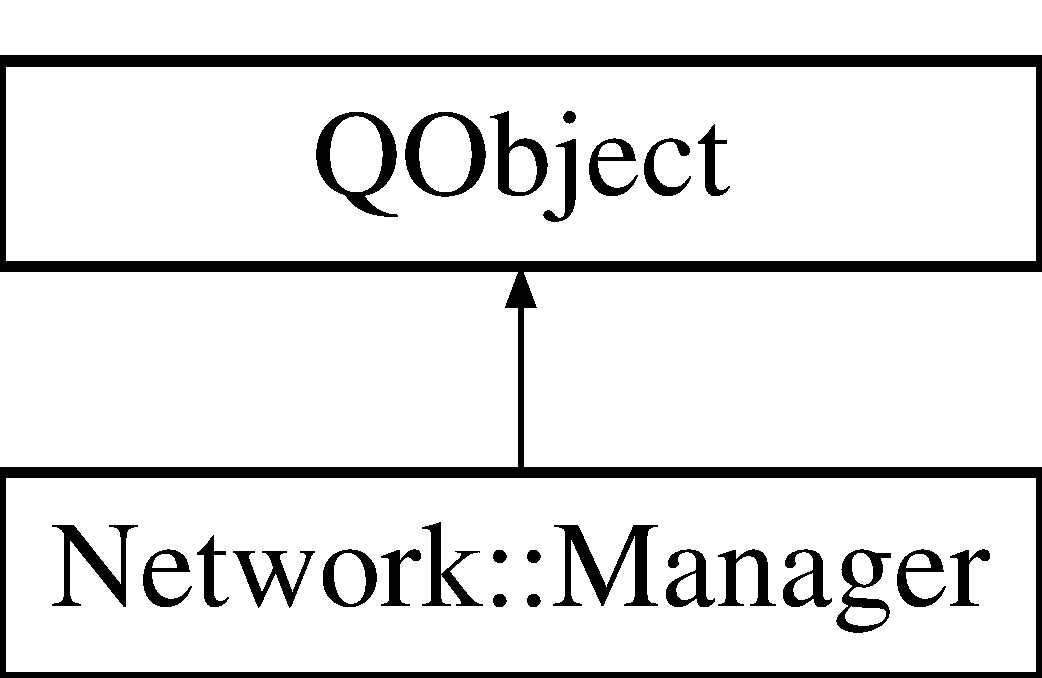
\includegraphics[height=2.000000cm]{classNetwork_1_1Manager}
\end{center}
\end{figure}
\subsection*{Public Slots}
\begin{DoxyCompactItemize}
\item 
\mbox{\Hypertarget{classNetwork_1_1Manager_aa8df583727aa598ee39e6de18b438abe}\label{classNetwork_1_1Manager_aa8df583727aa598ee39e6de18b438abe}} 
void {\bfseries get\+Resource} (const Q\+Url \&url)
\item 
\mbox{\Hypertarget{classNetwork_1_1Manager_a88e7de8604594cf6c2689e8b7a0a6e6e}\label{classNetwork_1_1Manager_a88e7de8604594cf6c2689e8b7a0a6e6e}} 
void {\bfseries post\+Resource} (const Q\+Url \&url, const Q\+Byte\+Array \&data)
\item 
\mbox{\Hypertarget{classNetwork_1_1Manager_adef1a35e5066157068800847c9366c09}\label{classNetwork_1_1Manager_adef1a35e5066157068800847c9366c09}} 
void {\bfseries delete\+Resource} (const Q\+Url \&url)
\item 
\mbox{\Hypertarget{classNetwork_1_1Manager_a42ef9df33cf238b62e66a5759c316432}\label{classNetwork_1_1Manager_a42ef9df33cf238b62e66a5759c316432}} 
void {\bfseries head\+Resource} (const Q\+Url \&url)
\end{DoxyCompactItemize}
\subsection*{Signals}
\begin{DoxyCompactItemize}
\item 
\mbox{\Hypertarget{classNetwork_1_1Manager_a1863c9a52ea6587387c8a688b92a2204}\label{classNetwork_1_1Manager_a1863c9a52ea6587387c8a688b92a2204}} 
void {\bfseries request\+Completed} (Q\+Network\+Reply $\ast$reply)
\item 
\mbox{\Hypertarget{classNetwork_1_1Manager_a4fd0af58f8fcd61b2c17d2dd368693c6}\label{classNetwork_1_1Manager_a4fd0af58f8fcd61b2c17d2dd368693c6}} 
Q\+List$<$ Q\+Ssl\+Error $>$ {\bfseries ssl\+Errors\+Received} (Q\+Network\+Reply $\ast$reply, Q\+List$<$ Q\+Ssl\+Error $>$ ssl\+Error)
\item 
\mbox{\Hypertarget{classNetwork_1_1Manager_a39de38077117c92e1e9d6aea325b9537}\label{classNetwork_1_1Manager_a39de38077117c92e1e9d6aea325b9537}} 
Q\+Network\+Access\+Manager\+::\+Network\+Accessibility {\bfseries network\+Accessible\+Changed} (Q\+Network\+Access\+Manager\+::\+Network\+Accessibility state)
\item 
\mbox{\Hypertarget{classNetwork_1_1Manager_ad8dd2cecf77ca5869e46b4268e6e0c9a}\label{classNetwork_1_1Manager_ad8dd2cecf77ca5869e46b4268e6e0c9a}} 
void {\bfseries user\+Agent\+Changed} ()
\item 
\mbox{\Hypertarget{classNetwork_1_1Manager_a1f37b9f5fe58a613d5095893e7c9ddb7}\label{classNetwork_1_1Manager_a1f37b9f5fe58a613d5095893e7c9ddb7}} 
void {\bfseries accept\+Header\+Changed} ()
\end{DoxyCompactItemize}
\subsection*{Public Member Functions}
\begin{DoxyCompactItemize}
\item 
\mbox{\Hypertarget{classNetwork_1_1Manager_aa4f7e5630c9c95932146f0f97eb38ca1}\label{classNetwork_1_1Manager_aa4f7e5630c9c95932146f0f97eb38ca1}} 
Q\+String {\bfseries user\+Agent} () const
\item 
\mbox{\Hypertarget{classNetwork_1_1Manager_acb21aaf997144be186e7e07043cd04ba}\label{classNetwork_1_1Manager_acb21aaf997144be186e7e07043cd04ba}} 
void {\bfseries set\+User\+Agent} (const Q\+String \&user\+Agent)
\item 
\mbox{\Hypertarget{classNetwork_1_1Manager_ac0db9092d325d920fff7a2d095cf506b}\label{classNetwork_1_1Manager_ac0db9092d325d920fff7a2d095cf506b}} 
Q\+String {\bfseries accept\+Header} () const
\item 
\mbox{\Hypertarget{classNetwork_1_1Manager_ab2c4f941034a92beae89f5657777f992}\label{classNetwork_1_1Manager_ab2c4f941034a92beae89f5657777f992}} 
void {\bfseries set\+Accept\+Header} (const Q\+String \&accept\+Header)
\end{DoxyCompactItemize}
\subsection*{Static Public Member Functions}
\begin{DoxyCompactItemize}
\item 
\mbox{\Hypertarget{classNetwork_1_1Manager_adeda284a39ae4c942656ec87295cf024}\label{classNetwork_1_1Manager_adeda284a39ae4c942656ec87295cf024}} 
static \mbox{\hyperlink{classNetwork_1_1Manager}{Manager}} $\ast$ {\bfseries get\+Instance} ()
\end{DoxyCompactItemize}
\subsection*{Private Member Functions}
\begin{DoxyCompactItemize}
\item 
\mbox{\Hypertarget{classNetwork_1_1Manager_ad3499eea3fd823034264277f9e0cf6a9}\label{classNetwork_1_1Manager_ad3499eea3fd823034264277f9e0cf6a9}} 
{\bfseries Manager} (Q\+Object $\ast$parent=nullptr)
\item 
\mbox{\Hypertarget{classNetwork_1_1Manager_aa9c1081a6e3ec9b937c3bbb9a7f7202f}\label{classNetwork_1_1Manager_aa9c1081a6e3ec9b937c3bbb9a7f7202f}} 
Q\+Network\+Request {\bfseries prepare\+Request} (const Q\+Url \&url)
\item 
\mbox{\Hypertarget{classNetwork_1_1Manager_a105b541b83fa32472b40730a885154ef}\label{classNetwork_1_1Manager_a105b541b83fa32472b40730a885154ef}} 
Q\+Network\+Access\+Manager $\ast$ {\bfseries Q\+N\+AM} () const
\item 
\mbox{\Hypertarget{classNetwork_1_1Manager_aaf5a945f52e51e357b53cacdc7319ab2}\label{classNetwork_1_1Manager_aaf5a945f52e51e357b53cacdc7319ab2}} 
void {\bfseries set\+Q\+N\+AM} (Q\+Network\+Access\+Manager $\ast$value)
\item 
\mbox{\Hypertarget{classNetwork_1_1Manager_a4aea14959afca0afd4b91208033da401}\label{classNetwork_1_1Manager_a4aea14959afca0afd4b91208033da401}} 
Q\+Abstract\+Network\+Cache $\ast$ {\bfseries cache} () const
\item 
\mbox{\Hypertarget{classNetwork_1_1Manager_ab73570326de530e3cdd09f6bf3f195d0}\label{classNetwork_1_1Manager_ab73570326de530e3cdd09f6bf3f195d0}} 
void {\bfseries set\+Cache} (Q\+Abstract\+Network\+Cache $\ast$cache)
\end{DoxyCompactItemize}
\subsection*{Static Private Member Functions}
\begin{DoxyCompactItemize}
\item 
\mbox{\Hypertarget{classNetwork_1_1Manager_a42c71474900c4d1e68740ae8d73db848}\label{classNetwork_1_1Manager_a42c71474900c4d1e68740ae8d73db848}} 
static \mbox{\hyperlink{classNetwork_1_1Manager}{Manager}} $\ast$ {\bfseries manager} ()
\item 
\mbox{\Hypertarget{classNetwork_1_1Manager_a1bc97c8b2dc5a4be751005d6a5dcf0a0}\label{classNetwork_1_1Manager_a1bc97c8b2dc5a4be751005d6a5dcf0a0}} 
static void {\bfseries set\+Manager} (const \mbox{\hyperlink{classNetwork_1_1Manager}{Manager}} $\ast$manager)
\end{DoxyCompactItemize}
\subsection*{Private Attributes}
\begin{DoxyCompactItemize}
\item 
\mbox{\Hypertarget{classNetwork_1_1Manager_a6f69f8099c8706abebd1a4497e5038f8}\label{classNetwork_1_1Manager_a6f69f8099c8706abebd1a4497e5038f8}} 
Q\+Network\+Access\+Manager $\ast$ {\bfseries m\+\_\+\+Q\+N\+AM}
\item 
\mbox{\Hypertarget{classNetwork_1_1Manager_aa99fb56d9b2a75b5f5a63a191002f461}\label{classNetwork_1_1Manager_aa99fb56d9b2a75b5f5a63a191002f461}} 
Q\+Abstract\+Network\+Cache $\ast$ {\bfseries m\+\_\+cache}
\item 
\mbox{\Hypertarget{classNetwork_1_1Manager_a59e8c58e1efd376525f400750ee87943}\label{classNetwork_1_1Manager_a59e8c58e1efd376525f400750ee87943}} 
Q\+String {\bfseries m\+\_\+user\+Agent}
\item 
\mbox{\Hypertarget{classNetwork_1_1Manager_a04138b3a1b6b6d9a0c8816de74ab50a2}\label{classNetwork_1_1Manager_a04138b3a1b6b6d9a0c8816de74ab50a2}} 
Q\+String {\bfseries m\+\_\+accept\+Header}
\end{DoxyCompactItemize}
\subsection*{Static Private Attributes}
\begin{DoxyCompactItemize}
\item 
\mbox{\Hypertarget{classNetwork_1_1Manager_a02ab401c85b17ffca2b9f3f69a4bae3b}\label{classNetwork_1_1Manager_a02ab401c85b17ffca2b9f3f69a4bae3b}} 
static \mbox{\hyperlink{classNetwork_1_1Manager}{Manager}} $\ast$ {\bfseries m\+\_\+instance} = nullptr
\end{DoxyCompactItemize}


The documentation for this class was generated from the following files\+:\begin{DoxyCompactItemize}
\item 
src/include/network/networkmanager.\+h\item 
src/network/\mbox{\hyperlink{networkmanager_8cpp}{networkmanager.\+cpp}}\end{DoxyCompactItemize}

\hypertarget{classDatabase_1_1Manager}{}\section{Database\+:\+:Manager Class Reference}
\label{classDatabase_1_1Manager}\index{Database\+::\+Manager@{Database\+::\+Manager}}


{\ttfamily \#include $<$databasemanager.\+h$>$}

Inheritance diagram for Database\+:\+:Manager\+:\begin{figure}[H]
\begin{center}
\leavevmode
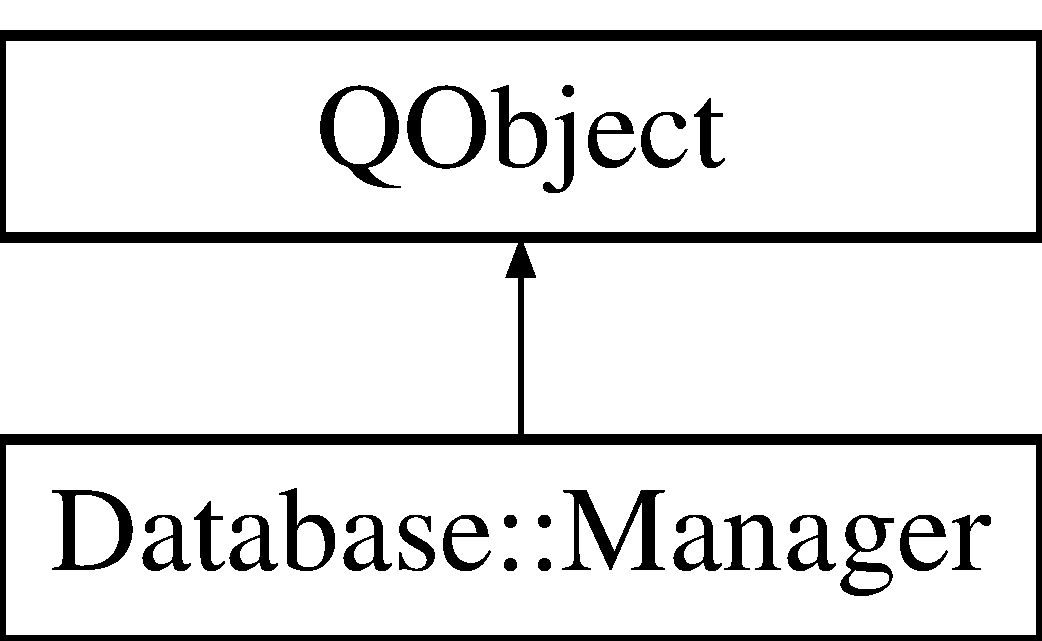
\includegraphics[height=2.000000cm]{classDatabase_1_1Manager}
\end{center}
\end{figure}
\subsection*{Public Member Functions}
\begin{DoxyCompactItemize}
\item 
bool \mbox{\hyperlink{classDatabase_1_1Manager_a0afd7a0884097a8dcff61b0444f39fb4}{execute}} (Q\+Sql\+Query \&query)
\item 
bool \mbox{\hyperlink{classDatabase_1_1Manager_adbe8be75b47c9770556464859bcc3017}{start\+Transaction}} ()
\item 
bool \mbox{\hyperlink{classDatabase_1_1Manager_a08dc190a448c555f8334bdd60d32b26e}{end\+Transaction}} ()
\item 
Q\+Sql\+Database \mbox{\hyperlink{classDatabase_1_1Manager_aecc5a00737bf6392cccda37a99138d8c}{database}} () const
\end{DoxyCompactItemize}
\subsection*{Static Public Member Functions}
\begin{DoxyCompactItemize}
\item 
static \mbox{\hyperlink{classDatabase_1_1Manager}{Manager}} $\ast$ \mbox{\hyperlink{classDatabase_1_1Manager_a6f8f8635c67e8d6e3ee86410006d22f3}{get\+Instance}} (const Q\+String \&path, Q\+Object $\ast$parent=nullptr)
\end{DoxyCompactItemize}
\subsection*{Private Member Functions}
\begin{DoxyCompactItemize}
\item 
\mbox{\hyperlink{classDatabase_1_1Manager_a3046834f78e2c3c5bce479b8eba31df4}{Manager}} (const Q\+String \&path, Q\+Object $\ast$parent)
\item 
void \mbox{\hyperlink{classDatabase_1_1Manager_af7f86ed5807bd6299fe4aa594b72013c}{set\+Database}} (const Q\+Sql\+Database \&\mbox{\hyperlink{classDatabase_1_1Manager_aecc5a00737bf6392cccda37a99138d8c}{database}})
\end{DoxyCompactItemize}
\subsection*{Private Attributes}
\begin{DoxyCompactItemize}
\item 
Q\+Sql\+Database \mbox{\hyperlink{classDatabase_1_1Manager_a4de33edd790c0d8320c0a2a5990f5169}{m\+\_\+database}}
\end{DoxyCompactItemize}
\subsection*{Static Private Attributes}
\begin{DoxyCompactItemize}
\item 
static \mbox{\hyperlink{classDatabase_1_1Manager}{Manager}} $\ast$ \mbox{\hyperlink{classDatabase_1_1Manager_a35e8446687862c34ae818636f953f54e}{m\+\_\+instance}} = nullptr
\end{DoxyCompactItemize}


\subsection{Constructor \& Destructor Documentation}
\mbox{\Hypertarget{classDatabase_1_1Manager_a3046834f78e2c3c5bce479b8eba31df4}\label{classDatabase_1_1Manager_a3046834f78e2c3c5bce479b8eba31df4}} 
\index{Database\+::\+Manager@{Database\+::\+Manager}!Manager@{Manager}}
\index{Manager@{Manager}!Database\+::\+Manager@{Database\+::\+Manager}}
\subsubsection{\texorpdfstring{Manager()}{Manager()}}
{\footnotesize\ttfamily Database\+::\+Manager\+::\+Manager (\begin{DoxyParamCaption}\item[{const Q\+String \&}]{path,  }\item[{Q\+Object $\ast$}]{parent }\end{DoxyParamCaption})\hspace{0.3cm}{\ttfamily [explicit]}, {\ttfamily [private]}}



\subsection{Member Function Documentation}
\mbox{\Hypertarget{classDatabase_1_1Manager_aecc5a00737bf6392cccda37a99138d8c}\label{classDatabase_1_1Manager_aecc5a00737bf6392cccda37a99138d8c}} 
\index{Database\+::\+Manager@{Database\+::\+Manager}!database@{database}}
\index{database@{database}!Database\+::\+Manager@{Database\+::\+Manager}}
\subsubsection{\texorpdfstring{database()}{database()}}
{\footnotesize\ttfamily Q\+Sql\+Database Database\+::\+Manager\+::database (\begin{DoxyParamCaption}{ }\end{DoxyParamCaption}) const}

\mbox{\Hypertarget{classDatabase_1_1Manager_a08dc190a448c555f8334bdd60d32b26e}\label{classDatabase_1_1Manager_a08dc190a448c555f8334bdd60d32b26e}} 
\index{Database\+::\+Manager@{Database\+::\+Manager}!end\+Transaction@{end\+Transaction}}
\index{end\+Transaction@{end\+Transaction}!Database\+::\+Manager@{Database\+::\+Manager}}
\subsubsection{\texorpdfstring{end\+Transaction()}{endTransaction()}}
{\footnotesize\ttfamily bool Database\+::\+Manager\+::end\+Transaction (\begin{DoxyParamCaption}{ }\end{DoxyParamCaption})}

\mbox{\Hypertarget{classDatabase_1_1Manager_a0afd7a0884097a8dcff61b0444f39fb4}\label{classDatabase_1_1Manager_a0afd7a0884097a8dcff61b0444f39fb4}} 
\index{Database\+::\+Manager@{Database\+::\+Manager}!execute@{execute}}
\index{execute@{execute}!Database\+::\+Manager@{Database\+::\+Manager}}
\subsubsection{\texorpdfstring{execute()}{execute()}}
{\footnotesize\ttfamily bool Database\+::\+Manager\+::execute (\begin{DoxyParamCaption}\item[{Q\+Sql\+Query \&}]{query }\end{DoxyParamCaption})}

\mbox{\Hypertarget{classDatabase_1_1Manager_a6f8f8635c67e8d6e3ee86410006d22f3}\label{classDatabase_1_1Manager_a6f8f8635c67e8d6e3ee86410006d22f3}} 
\index{Database\+::\+Manager@{Database\+::\+Manager}!get\+Instance@{get\+Instance}}
\index{get\+Instance@{get\+Instance}!Database\+::\+Manager@{Database\+::\+Manager}}
\subsubsection{\texorpdfstring{get\+Instance()}{getInstance()}}
{\footnotesize\ttfamily \mbox{\hyperlink{classDatabase_1_1Manager}{Database\+::\+Manager}} $\ast$ Database\+::\+Manager\+::get\+Instance (\begin{DoxyParamCaption}\item[{const Q\+String \&}]{path,  }\item[{Q\+Object $\ast$}]{parent = {\ttfamily nullptr} }\end{DoxyParamCaption})\hspace{0.3cm}{\ttfamily [static]}}

\mbox{\Hypertarget{classDatabase_1_1Manager_af7f86ed5807bd6299fe4aa594b72013c}\label{classDatabase_1_1Manager_af7f86ed5807bd6299fe4aa594b72013c}} 
\index{Database\+::\+Manager@{Database\+::\+Manager}!set\+Database@{set\+Database}}
\index{set\+Database@{set\+Database}!Database\+::\+Manager@{Database\+::\+Manager}}
\subsubsection{\texorpdfstring{set\+Database()}{setDatabase()}}
{\footnotesize\ttfamily void Database\+::\+Manager\+::set\+Database (\begin{DoxyParamCaption}\item[{const Q\+Sql\+Database \&}]{database }\end{DoxyParamCaption})\hspace{0.3cm}{\ttfamily [private]}}

\mbox{\Hypertarget{classDatabase_1_1Manager_adbe8be75b47c9770556464859bcc3017}\label{classDatabase_1_1Manager_adbe8be75b47c9770556464859bcc3017}} 
\index{Database\+::\+Manager@{Database\+::\+Manager}!start\+Transaction@{start\+Transaction}}
\index{start\+Transaction@{start\+Transaction}!Database\+::\+Manager@{Database\+::\+Manager}}
\subsubsection{\texorpdfstring{start\+Transaction()}{startTransaction()}}
{\footnotesize\ttfamily bool Database\+::\+Manager\+::start\+Transaction (\begin{DoxyParamCaption}{ }\end{DoxyParamCaption})}



\subsection{Member Data Documentation}
\mbox{\Hypertarget{classDatabase_1_1Manager_a4de33edd790c0d8320c0a2a5990f5169}\label{classDatabase_1_1Manager_a4de33edd790c0d8320c0a2a5990f5169}} 
\index{Database\+::\+Manager@{Database\+::\+Manager}!m\+\_\+database@{m\+\_\+database}}
\index{m\+\_\+database@{m\+\_\+database}!Database\+::\+Manager@{Database\+::\+Manager}}
\subsubsection{\texorpdfstring{m\+\_\+database}{m\_database}}
{\footnotesize\ttfamily Q\+Sql\+Database Database\+::\+Manager\+::m\+\_\+database\hspace{0.3cm}{\ttfamily [private]}}

\mbox{\Hypertarget{classDatabase_1_1Manager_a35e8446687862c34ae818636f953f54e}\label{classDatabase_1_1Manager_a35e8446687862c34ae818636f953f54e}} 
\index{Database\+::\+Manager@{Database\+::\+Manager}!m\+\_\+instance@{m\+\_\+instance}}
\index{m\+\_\+instance@{m\+\_\+instance}!Database\+::\+Manager@{Database\+::\+Manager}}
\subsubsection{\texorpdfstring{m\+\_\+instance}{m\_instance}}
{\footnotesize\ttfamily \mbox{\hyperlink{classDatabase_1_1Manager}{Database\+::\+Manager}} $\ast$ Database\+::\+Manager\+::m\+\_\+instance = nullptr\hspace{0.3cm}{\ttfamily [static]}, {\ttfamily [private]}}



The documentation for this class was generated from the following files\+:\begin{DoxyCompactItemize}
\item 
src/database/\mbox{\hyperlink{databasemanager_8h}{databasemanager.\+h}}\item 
src/database/\mbox{\hyperlink{databasemanager_8cpp}{databasemanager.\+cpp}}\end{DoxyCompactItemize}

\hypertarget{classCSA_1_1Message}{}\section{C\+SA\+:\+:Message Class Reference}
\label{classCSA_1_1Message}\index{C\+S\+A\+::\+Message@{C\+S\+A\+::\+Message}}


{\ttfamily \#include $<$csamessage.\+h$>$}

Inheritance diagram for C\+SA\+:\+:Message\+:\begin{figure}[H]
\begin{center}
\leavevmode
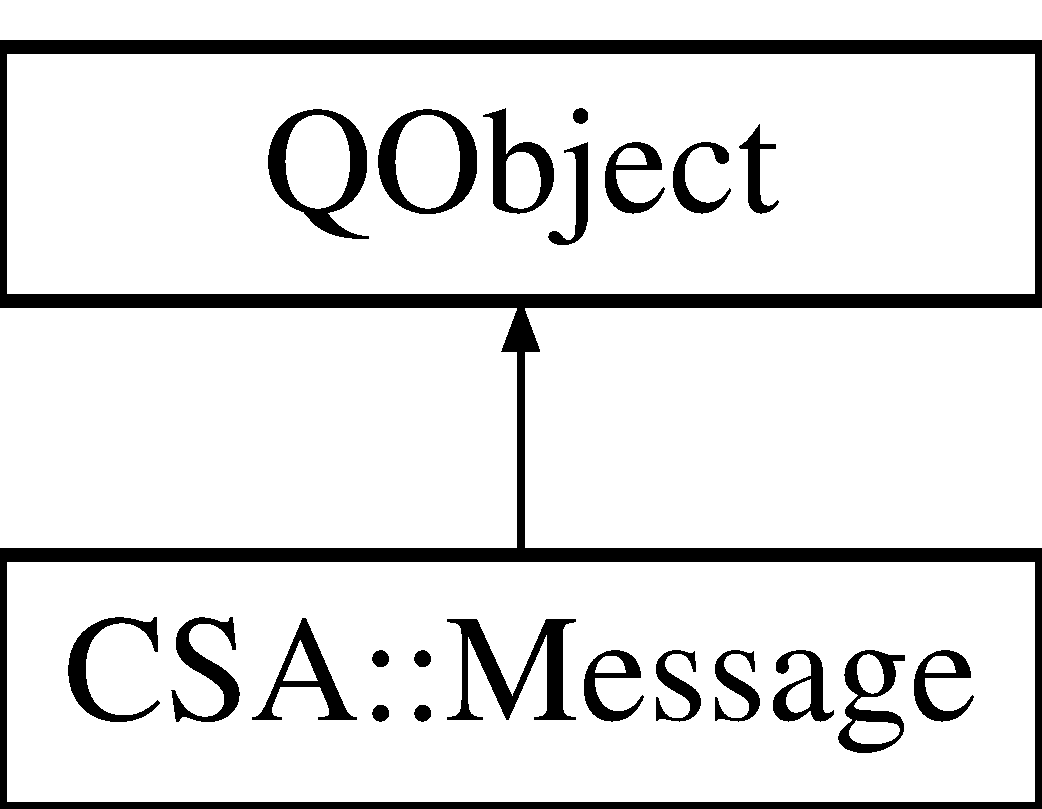
\includegraphics[height=2.000000cm]{classCSA_1_1Message}
\end{center}
\end{figure}
\subsection*{Signals}
\begin{DoxyCompactItemize}
\item 
void \mbox{\hyperlink{classCSA_1_1Message_a2d58350e147ba775ea6e4984d4ac0bd9}{header\+Changed}} ()
\item 
void \mbox{\hyperlink{classCSA_1_1Message_a3aa4f9f897726496236f8f44e62a2e98}{description\+Changed}} ()
\item 
void \mbox{\hyperlink{classCSA_1_1Message_a07926969b6de9fcea2a41de78d53a8db}{lead\+Changed}} ()
\item 
void \mbox{\hyperlink{classCSA_1_1Message_a570a510caf83d71d37b8e8a3d625be54}{link\+Changed}} ()
\end{DoxyCompactItemize}
\subsection*{Public Member Functions}
\begin{DoxyCompactItemize}
\item 
\mbox{\hyperlink{classCSA_1_1Message_aca2e81acce38bd7ac3e2b44669c41e9e}{Message}} (const Q\+String \&\mbox{\hyperlink{classCSA_1_1Message_a4400bbedbca391321c94e3620c743c0d}{header}}, const Q\+String \&\mbox{\hyperlink{classCSA_1_1Message_ad5ab91547afc7777c9921c2973418d19}{description}}, const Q\+String \&\mbox{\hyperlink{classCSA_1_1Message_ade0403777364c446f7cee8ba1897a75c}{lead}}, const Q\+Url \&\mbox{\hyperlink{classCSA_1_1Message_a7ddadacf05fdaa5d973025bc3892f517}{link}}, Q\+Object $\ast$parent=nullptr)
\item 
\mbox{\hyperlink{classCSA_1_1Message_ae1abb7c31a0f40f3601b7d2b21d2fec9}{Message}} (const Q\+String \&\mbox{\hyperlink{classCSA_1_1Message_a4400bbedbca391321c94e3620c743c0d}{header}}, const Q\+String \&\mbox{\hyperlink{classCSA_1_1Message_ad5ab91547afc7777c9921c2973418d19}{description}}, Q\+Object $\ast$parent=nullptr)
\item 
Q\+String \mbox{\hyperlink{classCSA_1_1Message_a4400bbedbca391321c94e3620c743c0d}{header}} () const
\item 
void \mbox{\hyperlink{classCSA_1_1Message_aaa162792bac73c4f20d718c546c7cf5d}{set\+Header}} (const Q\+String \&\mbox{\hyperlink{classCSA_1_1Message_a4400bbedbca391321c94e3620c743c0d}{header}})
\item 
Q\+String \mbox{\hyperlink{classCSA_1_1Message_ad5ab91547afc7777c9921c2973418d19}{description}} () const
\item 
void \mbox{\hyperlink{classCSA_1_1Message_a6f67e046c556922e1d3a477215f1bcec}{set\+Description}} (const Q\+String \&\mbox{\hyperlink{classCSA_1_1Message_ad5ab91547afc7777c9921c2973418d19}{description}})
\item 
Q\+String \mbox{\hyperlink{classCSA_1_1Message_ade0403777364c446f7cee8ba1897a75c}{lead}} () const
\item 
void \mbox{\hyperlink{classCSA_1_1Message_aa70caaac5d69af259fb838f0dd6fde01}{set\+Lead}} (const Q\+String \&\mbox{\hyperlink{classCSA_1_1Message_ade0403777364c446f7cee8ba1897a75c}{lead}})
\item 
Q\+Url \mbox{\hyperlink{classCSA_1_1Message_a7ddadacf05fdaa5d973025bc3892f517}{link}} () const
\item 
void \mbox{\hyperlink{classCSA_1_1Message_aa5443c2828acafd1b31d9c042dbc52f1}{set\+Link}} (const Q\+Url \&\mbox{\hyperlink{classCSA_1_1Message_a7ddadacf05fdaa5d973025bc3892f517}{link}})
\end{DoxyCompactItemize}
\subsection*{Private Attributes}
\begin{DoxyCompactItemize}
\item 
Q\+String \mbox{\hyperlink{classCSA_1_1Message_a3c274902f4b87b5acd6e15e60d8909eb}{m\+\_\+header}}
\item 
Q\+String \mbox{\hyperlink{classCSA_1_1Message_ae91f8d05186178670a26d8acf9279b14}{m\+\_\+description}}
\item 
Q\+String \mbox{\hyperlink{classCSA_1_1Message_a89d011c48a82f63384531d1af495ab79}{m\+\_\+lead}}
\item 
Q\+Url \mbox{\hyperlink{classCSA_1_1Message_a8d8f7f50df05a4f0ae80e9cd40c4435b}{m\+\_\+link}}
\end{DoxyCompactItemize}


\subsection{Constructor \& Destructor Documentation}
\mbox{\Hypertarget{classCSA_1_1Message_aca2e81acce38bd7ac3e2b44669c41e9e}\label{classCSA_1_1Message_aca2e81acce38bd7ac3e2b44669c41e9e}} 
\index{C\+S\+A\+::\+Message@{C\+S\+A\+::\+Message}!Message@{Message}}
\index{Message@{Message}!C\+S\+A\+::\+Message@{C\+S\+A\+::\+Message}}
\subsubsection{\texorpdfstring{Message()}{Message()}\hspace{0.1cm}{\footnotesize\ttfamily [1/2]}}
{\footnotesize\ttfamily C\+S\+A\+::\+Message\+::\+Message (\begin{DoxyParamCaption}\item[{const Q\+String \&}]{header,  }\item[{const Q\+String \&}]{description,  }\item[{const Q\+String \&}]{lead,  }\item[{const Q\+Url \&}]{link,  }\item[{Q\+Object $\ast$}]{parent = {\ttfamily nullptr} }\end{DoxyParamCaption})\hspace{0.3cm}{\ttfamily [explicit]}}

\mbox{\Hypertarget{classCSA_1_1Message_ae1abb7c31a0f40f3601b7d2b21d2fec9}\label{classCSA_1_1Message_ae1abb7c31a0f40f3601b7d2b21d2fec9}} 
\index{C\+S\+A\+::\+Message@{C\+S\+A\+::\+Message}!Message@{Message}}
\index{Message@{Message}!C\+S\+A\+::\+Message@{C\+S\+A\+::\+Message}}
\subsubsection{\texorpdfstring{Message()}{Message()}\hspace{0.1cm}{\footnotesize\ttfamily [2/2]}}
{\footnotesize\ttfamily C\+S\+A\+::\+Message\+::\+Message (\begin{DoxyParamCaption}\item[{const Q\+String \&}]{header,  }\item[{const Q\+String \&}]{description,  }\item[{Q\+Object $\ast$}]{parent = {\ttfamily nullptr} }\end{DoxyParamCaption})\hspace{0.3cm}{\ttfamily [explicit]}}



\subsection{Member Function Documentation}
\mbox{\Hypertarget{classCSA_1_1Message_ad5ab91547afc7777c9921c2973418d19}\label{classCSA_1_1Message_ad5ab91547afc7777c9921c2973418d19}} 
\index{C\+S\+A\+::\+Message@{C\+S\+A\+::\+Message}!description@{description}}
\index{description@{description}!C\+S\+A\+::\+Message@{C\+S\+A\+::\+Message}}
\subsubsection{\texorpdfstring{description()}{description()}}
{\footnotesize\ttfamily Q\+String C\+S\+A\+::\+Message\+::description (\begin{DoxyParamCaption}{ }\end{DoxyParamCaption}) const}

\mbox{\Hypertarget{classCSA_1_1Message_a3aa4f9f897726496236f8f44e62a2e98}\label{classCSA_1_1Message_a3aa4f9f897726496236f8f44e62a2e98}} 
\index{C\+S\+A\+::\+Message@{C\+S\+A\+::\+Message}!description\+Changed@{description\+Changed}}
\index{description\+Changed@{description\+Changed}!C\+S\+A\+::\+Message@{C\+S\+A\+::\+Message}}
\subsubsection{\texorpdfstring{description\+Changed}{descriptionChanged}}
{\footnotesize\ttfamily void C\+S\+A\+::\+Message\+::description\+Changed (\begin{DoxyParamCaption}{ }\end{DoxyParamCaption})\hspace{0.3cm}{\ttfamily [signal]}}

\mbox{\Hypertarget{classCSA_1_1Message_a4400bbedbca391321c94e3620c743c0d}\label{classCSA_1_1Message_a4400bbedbca391321c94e3620c743c0d}} 
\index{C\+S\+A\+::\+Message@{C\+S\+A\+::\+Message}!header@{header}}
\index{header@{header}!C\+S\+A\+::\+Message@{C\+S\+A\+::\+Message}}
\subsubsection{\texorpdfstring{header()}{header()}}
{\footnotesize\ttfamily Q\+String C\+S\+A\+::\+Message\+::header (\begin{DoxyParamCaption}{ }\end{DoxyParamCaption}) const}

\mbox{\Hypertarget{classCSA_1_1Message_a2d58350e147ba775ea6e4984d4ac0bd9}\label{classCSA_1_1Message_a2d58350e147ba775ea6e4984d4ac0bd9}} 
\index{C\+S\+A\+::\+Message@{C\+S\+A\+::\+Message}!header\+Changed@{header\+Changed}}
\index{header\+Changed@{header\+Changed}!C\+S\+A\+::\+Message@{C\+S\+A\+::\+Message}}
\subsubsection{\texorpdfstring{header\+Changed}{headerChanged}}
{\footnotesize\ttfamily void C\+S\+A\+::\+Message\+::header\+Changed (\begin{DoxyParamCaption}{ }\end{DoxyParamCaption})\hspace{0.3cm}{\ttfamily [signal]}}

\mbox{\Hypertarget{classCSA_1_1Message_ade0403777364c446f7cee8ba1897a75c}\label{classCSA_1_1Message_ade0403777364c446f7cee8ba1897a75c}} 
\index{C\+S\+A\+::\+Message@{C\+S\+A\+::\+Message}!lead@{lead}}
\index{lead@{lead}!C\+S\+A\+::\+Message@{C\+S\+A\+::\+Message}}
\subsubsection{\texorpdfstring{lead()}{lead()}}
{\footnotesize\ttfamily Q\+String C\+S\+A\+::\+Message\+::lead (\begin{DoxyParamCaption}{ }\end{DoxyParamCaption}) const}

\mbox{\Hypertarget{classCSA_1_1Message_a07926969b6de9fcea2a41de78d53a8db}\label{classCSA_1_1Message_a07926969b6de9fcea2a41de78d53a8db}} 
\index{C\+S\+A\+::\+Message@{C\+S\+A\+::\+Message}!lead\+Changed@{lead\+Changed}}
\index{lead\+Changed@{lead\+Changed}!C\+S\+A\+::\+Message@{C\+S\+A\+::\+Message}}
\subsubsection{\texorpdfstring{lead\+Changed}{leadChanged}}
{\footnotesize\ttfamily void C\+S\+A\+::\+Message\+::lead\+Changed (\begin{DoxyParamCaption}{ }\end{DoxyParamCaption})\hspace{0.3cm}{\ttfamily [signal]}}

\mbox{\Hypertarget{classCSA_1_1Message_a7ddadacf05fdaa5d973025bc3892f517}\label{classCSA_1_1Message_a7ddadacf05fdaa5d973025bc3892f517}} 
\index{C\+S\+A\+::\+Message@{C\+S\+A\+::\+Message}!link@{link}}
\index{link@{link}!C\+S\+A\+::\+Message@{C\+S\+A\+::\+Message}}
\subsubsection{\texorpdfstring{link()}{link()}}
{\footnotesize\ttfamily Q\+Url C\+S\+A\+::\+Message\+::link (\begin{DoxyParamCaption}{ }\end{DoxyParamCaption}) const}

\mbox{\Hypertarget{classCSA_1_1Message_a570a510caf83d71d37b8e8a3d625be54}\label{classCSA_1_1Message_a570a510caf83d71d37b8e8a3d625be54}} 
\index{C\+S\+A\+::\+Message@{C\+S\+A\+::\+Message}!link\+Changed@{link\+Changed}}
\index{link\+Changed@{link\+Changed}!C\+S\+A\+::\+Message@{C\+S\+A\+::\+Message}}
\subsubsection{\texorpdfstring{link\+Changed}{linkChanged}}
{\footnotesize\ttfamily void C\+S\+A\+::\+Message\+::link\+Changed (\begin{DoxyParamCaption}{ }\end{DoxyParamCaption})\hspace{0.3cm}{\ttfamily [signal]}}

\mbox{\Hypertarget{classCSA_1_1Message_a6f67e046c556922e1d3a477215f1bcec}\label{classCSA_1_1Message_a6f67e046c556922e1d3a477215f1bcec}} 
\index{C\+S\+A\+::\+Message@{C\+S\+A\+::\+Message}!set\+Description@{set\+Description}}
\index{set\+Description@{set\+Description}!C\+S\+A\+::\+Message@{C\+S\+A\+::\+Message}}
\subsubsection{\texorpdfstring{set\+Description()}{setDescription()}}
{\footnotesize\ttfamily void C\+S\+A\+::\+Message\+::set\+Description (\begin{DoxyParamCaption}\item[{const Q\+String \&}]{description }\end{DoxyParamCaption})}

\mbox{\Hypertarget{classCSA_1_1Message_aaa162792bac73c4f20d718c546c7cf5d}\label{classCSA_1_1Message_aaa162792bac73c4f20d718c546c7cf5d}} 
\index{C\+S\+A\+::\+Message@{C\+S\+A\+::\+Message}!set\+Header@{set\+Header}}
\index{set\+Header@{set\+Header}!C\+S\+A\+::\+Message@{C\+S\+A\+::\+Message}}
\subsubsection{\texorpdfstring{set\+Header()}{setHeader()}}
{\footnotesize\ttfamily void C\+S\+A\+::\+Message\+::set\+Header (\begin{DoxyParamCaption}\item[{const Q\+String \&}]{header }\end{DoxyParamCaption})}

\mbox{\Hypertarget{classCSA_1_1Message_aa70caaac5d69af259fb838f0dd6fde01}\label{classCSA_1_1Message_aa70caaac5d69af259fb838f0dd6fde01}} 
\index{C\+S\+A\+::\+Message@{C\+S\+A\+::\+Message}!set\+Lead@{set\+Lead}}
\index{set\+Lead@{set\+Lead}!C\+S\+A\+::\+Message@{C\+S\+A\+::\+Message}}
\subsubsection{\texorpdfstring{set\+Lead()}{setLead()}}
{\footnotesize\ttfamily void C\+S\+A\+::\+Message\+::set\+Lead (\begin{DoxyParamCaption}\item[{const Q\+String \&}]{lead }\end{DoxyParamCaption})}

\mbox{\Hypertarget{classCSA_1_1Message_aa5443c2828acafd1b31d9c042dbc52f1}\label{classCSA_1_1Message_aa5443c2828acafd1b31d9c042dbc52f1}} 
\index{C\+S\+A\+::\+Message@{C\+S\+A\+::\+Message}!set\+Link@{set\+Link}}
\index{set\+Link@{set\+Link}!C\+S\+A\+::\+Message@{C\+S\+A\+::\+Message}}
\subsubsection{\texorpdfstring{set\+Link()}{setLink()}}
{\footnotesize\ttfamily void C\+S\+A\+::\+Message\+::set\+Link (\begin{DoxyParamCaption}\item[{const Q\+Url \&}]{link }\end{DoxyParamCaption})}



\subsection{Member Data Documentation}
\mbox{\Hypertarget{classCSA_1_1Message_ae91f8d05186178670a26d8acf9279b14}\label{classCSA_1_1Message_ae91f8d05186178670a26d8acf9279b14}} 
\index{C\+S\+A\+::\+Message@{C\+S\+A\+::\+Message}!m\+\_\+description@{m\+\_\+description}}
\index{m\+\_\+description@{m\+\_\+description}!C\+S\+A\+::\+Message@{C\+S\+A\+::\+Message}}
\subsubsection{\texorpdfstring{m\+\_\+description}{m\_description}}
{\footnotesize\ttfamily Q\+String C\+S\+A\+::\+Message\+::m\+\_\+description\hspace{0.3cm}{\ttfamily [private]}}

\mbox{\Hypertarget{classCSA_1_1Message_a3c274902f4b87b5acd6e15e60d8909eb}\label{classCSA_1_1Message_a3c274902f4b87b5acd6e15e60d8909eb}} 
\index{C\+S\+A\+::\+Message@{C\+S\+A\+::\+Message}!m\+\_\+header@{m\+\_\+header}}
\index{m\+\_\+header@{m\+\_\+header}!C\+S\+A\+::\+Message@{C\+S\+A\+::\+Message}}
\subsubsection{\texorpdfstring{m\+\_\+header}{m\_header}}
{\footnotesize\ttfamily Q\+String C\+S\+A\+::\+Message\+::m\+\_\+header\hspace{0.3cm}{\ttfamily [private]}}

\mbox{\Hypertarget{classCSA_1_1Message_a89d011c48a82f63384531d1af495ab79}\label{classCSA_1_1Message_a89d011c48a82f63384531d1af495ab79}} 
\index{C\+S\+A\+::\+Message@{C\+S\+A\+::\+Message}!m\+\_\+lead@{m\+\_\+lead}}
\index{m\+\_\+lead@{m\+\_\+lead}!C\+S\+A\+::\+Message@{C\+S\+A\+::\+Message}}
\subsubsection{\texorpdfstring{m\+\_\+lead}{m\_lead}}
{\footnotesize\ttfamily Q\+String C\+S\+A\+::\+Message\+::m\+\_\+lead\hspace{0.3cm}{\ttfamily [private]}}

\mbox{\Hypertarget{classCSA_1_1Message_a8d8f7f50df05a4f0ae80e9cd40c4435b}\label{classCSA_1_1Message_a8d8f7f50df05a4f0ae80e9cd40c4435b}} 
\index{C\+S\+A\+::\+Message@{C\+S\+A\+::\+Message}!m\+\_\+link@{m\+\_\+link}}
\index{m\+\_\+link@{m\+\_\+link}!C\+S\+A\+::\+Message@{C\+S\+A\+::\+Message}}
\subsubsection{\texorpdfstring{m\+\_\+link}{m\_link}}
{\footnotesize\ttfamily Q\+Url C\+S\+A\+::\+Message\+::m\+\_\+link\hspace{0.3cm}{\ttfamily [private]}}



The documentation for this class was generated from the following files\+:\begin{DoxyCompactItemize}
\item 
src/linkedconnections/csa/\mbox{\hyperlink{csamessage_8h}{csamessage.\+h}}\item 
src/linkedconnections/csa/\mbox{\hyperlink{csamessage_8cpp}{csamessage.\+cpp}}\end{DoxyCompactItemize}

\hypertarget{classCSA_1_1NullStation}{}\section{C\+SA\+:\+:Null\+Station Class Reference}
\label{classCSA_1_1NullStation}\index{C\+S\+A\+::\+Null\+Station@{C\+S\+A\+::\+Null\+Station}}


{\ttfamily \#include $<$csanullstation.\+h$>$}

Inheritance diagram for C\+SA\+:\+:Null\+Station\+:\begin{figure}[H]
\begin{center}
\leavevmode
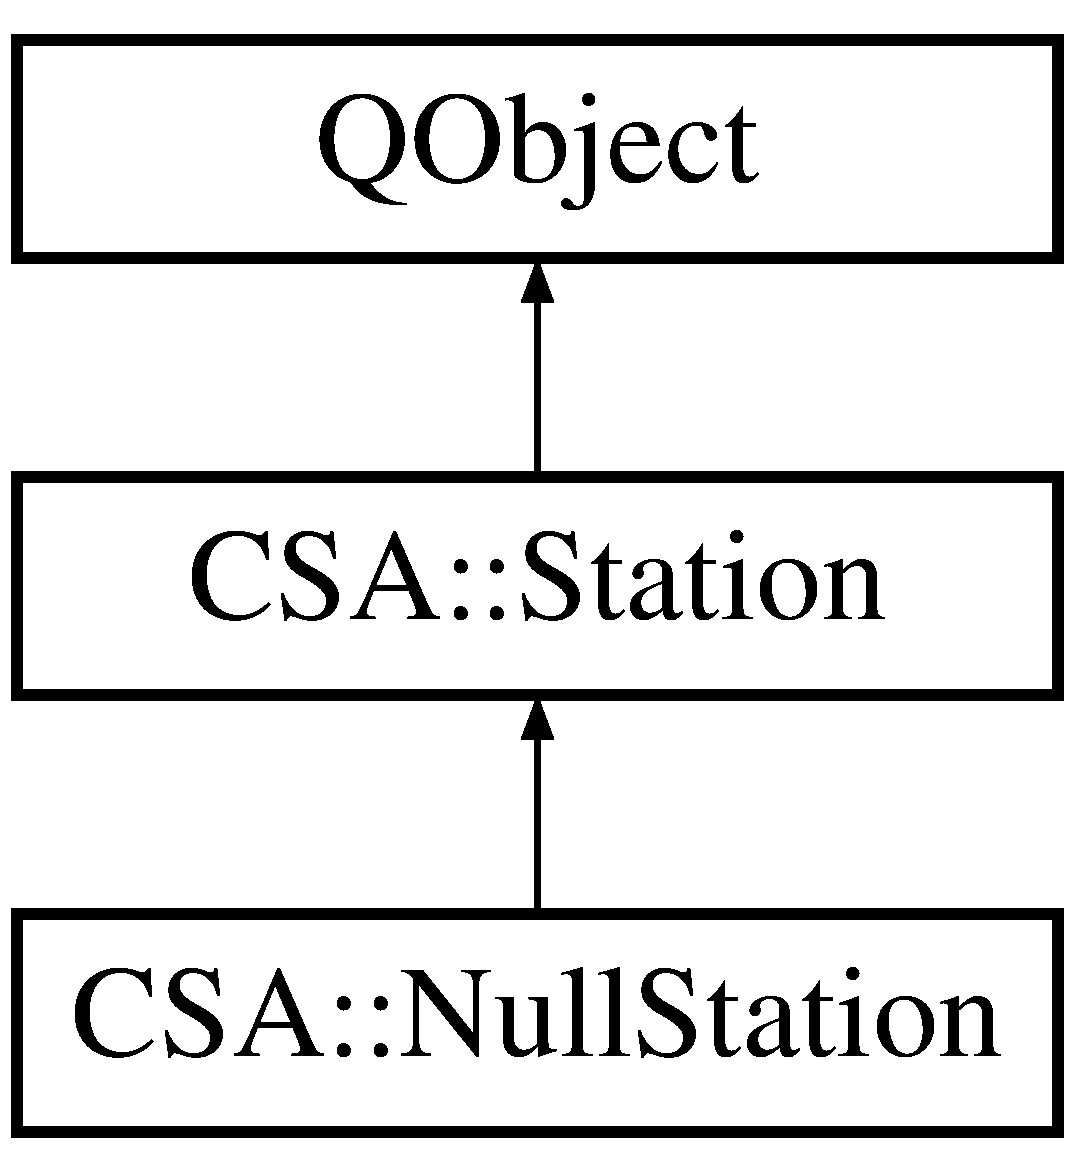
\includegraphics[height=3.000000cm]{classCSA_1_1NullStation}
\end{center}
\end{figure}
\subsection*{Static Public Member Functions}
\begin{DoxyCompactItemize}
\item 
static \mbox{\hyperlink{classCSA_1_1NullStation}{Null\+Station}} $\ast$ \mbox{\hyperlink{classCSA_1_1NullStation_a5e3c53a70b02d55f910d100574f3e461}{get\+Instance}} (Q\+Object $\ast$parent=nullptr)
\end{DoxyCompactItemize}
\subsection*{Private Member Functions}
\begin{DoxyCompactItemize}
\item 
\mbox{\hyperlink{classCSA_1_1NullStation_ac383e83e8ad47350e82b68a7c6e7b980}{Null\+Station}} (const Q\+Url \&\mbox{\hyperlink{classCSA_1_1Station_addca2c54d5e9ce61c4ef9c3ee9ff4100}{uri}}, const Q\+Map$<$ Q\+Locale\+::\+Language, Q\+String $>$ \&\mbox{\hyperlink{classCSA_1_1Station_ad4442763fc108cde8368260119c007da}{name}}, const Q\+Locale\+::\+Country \&\mbox{\hyperlink{classCSA_1_1Station_ac54cea5fde8ba6e2367f0317965d9147}{country}}, const Q\+Geo\+Coordinate \&\mbox{\hyperlink{classCSA_1_1Station_a94249de9cc38d704eb6e77aca24daaea}{position}}, const Q\+Geo\+Address \&\mbox{\hyperlink{classCSA_1_1Station_a82482b7595c3a587be4d2473eeff2d42}{address}}, const bool \&\mbox{\hyperlink{classCSA_1_1Station_a9e3f2a57d2e3793a375b8c3a7182ec7b}{has\+Ticket\+Vending\+Machine}}, const bool \&\mbox{\hyperlink{classCSA_1_1Station_aaa684a525fd9cef75108a1fe52ea5053}{has\+Luggage\+Lockers}}, const bool \&\mbox{\hyperlink{classCSA_1_1Station_a89e7b6e8612bef71f123986164aa1ba4}{has\+Free\+Parking}}, const bool \&\mbox{\hyperlink{classCSA_1_1Station_a886f635564cc01430552529d07527343}{has\+Taxi}}, const bool \&\mbox{\hyperlink{classCSA_1_1Station_a659f45a05d2920e6141db42d0fe9c7ff}{has\+Bicycle\+Spots}}, const bool \&\mbox{\hyperlink{classCSA_1_1Station_af3be093b4e7bbad8c76de068804765e6}{has\+Blue\+Bike}}, const bool \&\mbox{\hyperlink{classCSA_1_1Station_a02fa7a1b47bc2b7170f8817d49d6f992}{has\+Bus}}, const bool \&\mbox{\hyperlink{classCSA_1_1Station_ab01f8eb60d105cd77b5489e5b6746671}{has\+Tram}}, const bool \&\mbox{\hyperlink{classCSA_1_1Station_af51e8389ffadbbe19ef2d485434d94b5}{has\+Metro}}, const bool \&\mbox{\hyperlink{classCSA_1_1Station_a72be06dc6901f2707b22aa055e783a9f}{has\+Wheelchair\+Available}}, const bool \&\mbox{\hyperlink{classCSA_1_1Station_a07526fe7c2d2f0c47b8920d830f2935c}{has\+Ramp}}, const qint16 \&\mbox{\hyperlink{classCSA_1_1Station_a89962b963e33d1a5db45f22d6a60834e}{disabled\+Parking\+Spots}}, const bool \&\mbox{\hyperlink{classCSA_1_1Station_a883e232e28352571f41095b31e3cac0e}{has\+Elevated\+Platform}}, const bool \&\mbox{\hyperlink{classCSA_1_1Station_ae6fa7ccf3c6ca7e819d5e795841afb08}{has\+Escalator\+Up}}, const bool \&\mbox{\hyperlink{classCSA_1_1Station_ac0cb1e889a3c323dca9679902a9ac1c8}{has\+Escalator\+Down}}, const bool \&\mbox{\hyperlink{classCSA_1_1Station_a7924a558376c91a293e0bfe0cc76c13b}{has\+Elevator\+Platform}}, const bool \&\mbox{\hyperlink{classCSA_1_1Station_ae60274e5ab0ce2e983067122900389a4}{has\+Hearing\+Aid\+Signal}}, const Q\+Map$<$ \mbox{\hyperlink{classCSA_1_1Station_aa160d0de40db0583099b5986dea1cd67}{C\+S\+A\+::\+Station\+::\+Day}}, Q\+Pair$<$ Q\+Time, Q\+Time $>$$>$ \&\mbox{\hyperlink{classCSA_1_1Station_aafe81d261ad07910a07dab3e21264174}{opening\+Hours}}, const qreal \&\mbox{\hyperlink{classCSA_1_1Station_aa8f1c3bfa7b4a3ad9ccc805ff7a2b931}{average\+Stop\+Times}}, Q\+Object $\ast$parent=nullptr)
\end{DoxyCompactItemize}
\subsection*{Static Private Attributes}
\begin{DoxyCompactItemize}
\item 
static \mbox{\hyperlink{classCSA_1_1NullStation}{C\+S\+A\+::\+Null\+Station}} $\ast$ \mbox{\hyperlink{classCSA_1_1NullStation_a691ee7698fd8e06c982daf1c8daf1e75}{m\+\_\+instance}} = nullptr
\end{DoxyCompactItemize}
\subsection*{Additional Inherited Members}


\subsection{Constructor \& Destructor Documentation}
\mbox{\Hypertarget{classCSA_1_1NullStation_ac383e83e8ad47350e82b68a7c6e7b980}\label{classCSA_1_1NullStation_ac383e83e8ad47350e82b68a7c6e7b980}} 
\index{C\+S\+A\+::\+Null\+Station@{C\+S\+A\+::\+Null\+Station}!Null\+Station@{Null\+Station}}
\index{Null\+Station@{Null\+Station}!C\+S\+A\+::\+Null\+Station@{C\+S\+A\+::\+Null\+Station}}
\subsubsection{\texorpdfstring{Null\+Station()}{NullStation()}}
{\footnotesize\ttfamily C\+S\+A\+::\+Null\+Station\+::\+Null\+Station (\begin{DoxyParamCaption}\item[{const Q\+Url \&}]{uri,  }\item[{const Q\+Map$<$ Q\+Locale\+::\+Language, Q\+String $>$ \&}]{name,  }\item[{const Q\+Locale\+::\+Country \&}]{country,  }\item[{const Q\+Geo\+Coordinate \&}]{position,  }\item[{const Q\+Geo\+Address \&}]{address,  }\item[{const bool \&}]{has\+Ticket\+Vending\+Machine,  }\item[{const bool \&}]{has\+Luggage\+Lockers,  }\item[{const bool \&}]{has\+Free\+Parking,  }\item[{const bool \&}]{has\+Taxi,  }\item[{const bool \&}]{has\+Bicycle\+Spots,  }\item[{const bool \&}]{has\+Blue\+Bike,  }\item[{const bool \&}]{has\+Bus,  }\item[{const bool \&}]{has\+Tram,  }\item[{const bool \&}]{has\+Metro,  }\item[{const bool \&}]{has\+Wheelchair\+Available,  }\item[{const bool \&}]{has\+Ramp,  }\item[{const qint16 \&}]{disabled\+Parking\+Spots,  }\item[{const bool \&}]{has\+Elevated\+Platform,  }\item[{const bool \&}]{has\+Escalator\+Up,  }\item[{const bool \&}]{has\+Escalator\+Down,  }\item[{const bool \&}]{has\+Elevator\+Platform,  }\item[{const bool \&}]{has\+Hearing\+Aid\+Signal,  }\item[{const Q\+Map$<$ \mbox{\hyperlink{classCSA_1_1Station_aa160d0de40db0583099b5986dea1cd67}{C\+S\+A\+::\+Station\+::\+Day}}, Q\+Pair$<$ Q\+Time, Q\+Time $>$$>$ \&}]{opening\+Hours,  }\item[{const qreal \&}]{average\+Stop\+Times,  }\item[{Q\+Object $\ast$}]{parent = {\ttfamily nullptr} }\end{DoxyParamCaption})\hspace{0.3cm}{\ttfamily [explicit]}, {\ttfamily [private]}}



\subsection{Member Function Documentation}
\mbox{\Hypertarget{classCSA_1_1NullStation_a5e3c53a70b02d55f910d100574f3e461}\label{classCSA_1_1NullStation_a5e3c53a70b02d55f910d100574f3e461}} 
\index{C\+S\+A\+::\+Null\+Station@{C\+S\+A\+::\+Null\+Station}!get\+Instance@{get\+Instance}}
\index{get\+Instance@{get\+Instance}!C\+S\+A\+::\+Null\+Station@{C\+S\+A\+::\+Null\+Station}}
\subsubsection{\texorpdfstring{get\+Instance()}{getInstance()}}
{\footnotesize\ttfamily \mbox{\hyperlink{classCSA_1_1NullStation}{C\+S\+A\+::\+Null\+Station}} $\ast$ C\+S\+A\+::\+Null\+Station\+::get\+Instance (\begin{DoxyParamCaption}\item[{Q\+Object $\ast$}]{parent = {\ttfamily nullptr} }\end{DoxyParamCaption})\hspace{0.3cm}{\ttfamily [static]}}



\subsection{Member Data Documentation}
\mbox{\Hypertarget{classCSA_1_1NullStation_a691ee7698fd8e06c982daf1c8daf1e75}\label{classCSA_1_1NullStation_a691ee7698fd8e06c982daf1c8daf1e75}} 
\index{C\+S\+A\+::\+Null\+Station@{C\+S\+A\+::\+Null\+Station}!m\+\_\+instance@{m\+\_\+instance}}
\index{m\+\_\+instance@{m\+\_\+instance}!C\+S\+A\+::\+Null\+Station@{C\+S\+A\+::\+Null\+Station}}
\subsubsection{\texorpdfstring{m\+\_\+instance}{m\_instance}}
{\footnotesize\ttfamily \mbox{\hyperlink{classCSA_1_1NullStation}{C\+S\+A\+::\+Null\+Station}} $\ast$ C\+S\+A\+::\+Null\+Station\+::m\+\_\+instance = nullptr\hspace{0.3cm}{\ttfamily [static]}, {\ttfamily [private]}}



The documentation for this class was generated from the following files\+:\begin{DoxyCompactItemize}
\item 
src/linkedconnections/csa/\mbox{\hyperlink{csanullstation_8h}{csanullstation.\+h}}\item 
src/linkedconnections/csa/\mbox{\hyperlink{csanullstation_8cpp}{csanullstation.\+cpp}}\end{DoxyCompactItemize}

\hypertarget{classOS}{}\section{OS Class Reference}
\label{classOS}\index{OS@{OS}}
Inheritance diagram for OS\+:\begin{figure}[H]
\begin{center}
\leavevmode
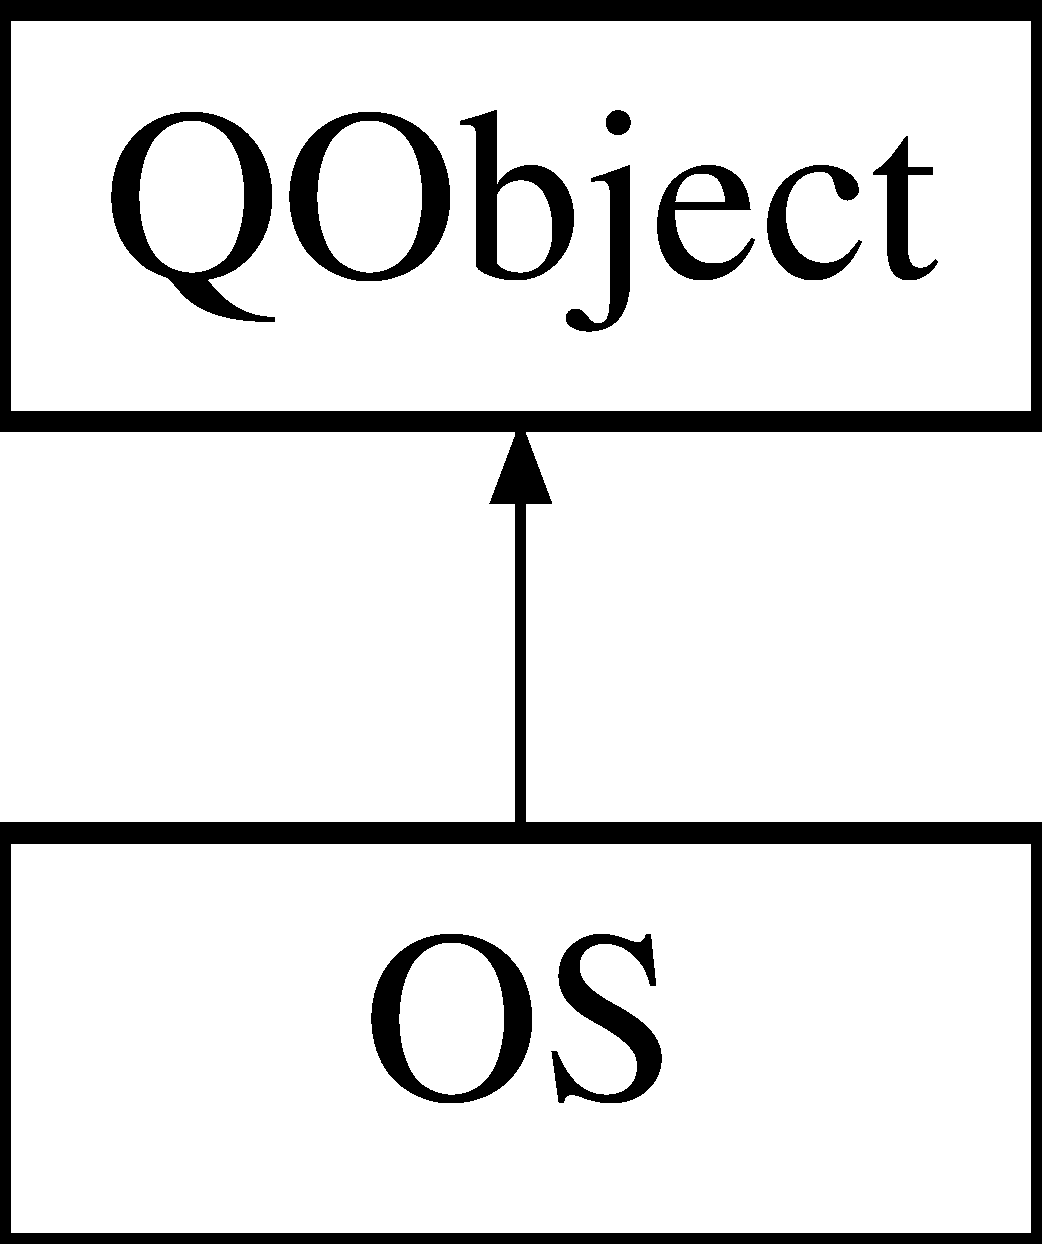
\includegraphics[height=2.000000cm]{classOS}
\end{center}
\end{figure}
\subsection*{Signals}
\begin{DoxyCompactItemize}
\item 
\mbox{\Hypertarget{classOS_a58369b88b24b1701b020bd0971d99c03}\label{classOS_a58369b88b24b1701b020bd0971d99c03}} 
void {\bfseries release\+Changed} ()
\item 
\mbox{\Hypertarget{classOS_a2bb282eb19c9eaa0c787dabc434a9fca}\label{classOS_a2bb282eb19c9eaa0c787dabc434a9fca}} 
void {\bfseries version\+Changed} ()
\item 
\mbox{\Hypertarget{classOS_ad55c57724a077d427b89ede6e1f8b235}\label{classOS_ad55c57724a077d427b89ede6e1f8b235}} 
void {\bfseries app\+Name\+Changed} ()
\item 
\mbox{\Hypertarget{classOS_a21d29e6b9eef2bccc62db0d29d56b4c5}\label{classOS_a21d29e6b9eef2bccc62db0d29d56b4c5}} 
void {\bfseries app\+Name\+Pretty\+Changed} ()
\item 
\mbox{\Hypertarget{classOS_a39f7a3688e008fde1008e6b7e5b5ebcb}\label{classOS_a39f7a3688e008fde1008e6b7e5b5ebcb}} 
void {\bfseries app\+Version\+Changed} ()
\item 
\mbox{\Hypertarget{classOS_a0ecbe56e6ec612ba6f78af5086505751}\label{classOS_a0ecbe56e6ec612ba6f78af5086505751}} 
void {\bfseries devicepixelratio\+Changed} ()
\end{DoxyCompactItemize}
\subsection*{Public Member Functions}
\begin{DoxyCompactItemize}
\item 
\mbox{\Hypertarget{classOS_ac21113cbcd347809f657c6a27a0278f6}\label{classOS_ac21113cbcd347809f657c6a27a0278f6}} 
Q\+\_\+\+I\+N\+V\+O\+K\+A\+B\+LE void {\bfseries create\+Notification} (Q\+String title, Q\+String text, Q\+String feedback, Q\+String category)
\item 
\mbox{\Hypertarget{classOS_a949a6aa1c2f8cd63d27cd6b8869da8fc}\label{classOS_a949a6aa1c2f8cd63d27cd6b8869da8fc}} 
Q\+\_\+\+I\+N\+V\+O\+K\+A\+B\+LE void {\bfseries create\+Toaster} (Q\+String text, Q\+String icon, Q\+String category)
\item 
\mbox{\Hypertarget{classOS_a8ab936784f48408f14ad73f10ae5afb8}\label{classOS_a8ab936784f48408f14ad73f10ae5afb8}} 
Q\+\_\+\+I\+N\+V\+O\+K\+A\+B\+LE void {\bfseries close\+Notification\+By\+Category} (Q\+String category)
\item 
\mbox{\Hypertarget{classOS_a8cc3c6824e01ae679819c8c3daf7842e}\label{classOS_a8cc3c6824e01ae679819c8c3daf7842e}} 
Q\+\_\+\+I\+N\+V\+O\+K\+A\+B\+LE void {\bfseries close\+Notification\+By\+Replaces\+Id} (Q\+String replaces\+Id)
\item 
\mbox{\Hypertarget{classOS_a16c6da56d519e2c2bccbdeaf5c4ff29b}\label{classOS_a16c6da56d519e2c2bccbdeaf5c4ff29b}} 
Q\+\_\+\+I\+N\+V\+O\+K\+A\+B\+LE void {\bfseries close\+Notification\+All} ()
\item 
\mbox{\Hypertarget{classOS_a1d00cd418f5d83cc174492326f7cd604}\label{classOS_a1d00cd418f5d83cc174492326f7cd604}} 
Q\+String {\bfseries release} ()
\item 
\mbox{\Hypertarget{classOS_a4cd043becb244d8f40bdcc55c0417a71}\label{classOS_a4cd043becb244d8f40bdcc55c0417a71}} 
Q\+String {\bfseries version} ()
\item 
\mbox{\Hypertarget{classOS_a800e819bbb7aa20945893d138b2a1bb3}\label{classOS_a800e819bbb7aa20945893d138b2a1bb3}} 
Q\+String {\bfseries device} ()
\item 
\mbox{\Hypertarget{classOS_a44dcb6a2ee199b111d98eb1e364bfef7}\label{classOS_a44dcb6a2ee199b111d98eb1e364bfef7}} 
Q\+String {\bfseries cache\+Location} ()
\item 
\mbox{\Hypertarget{classOS_ae8a69330410d1b615443920baa19cea7}\label{classOS_ae8a69330410d1b615443920baa19cea7}} 
Q\+String {\bfseries data\+Location} ()
\item 
\mbox{\Hypertarget{classOS_ae319d1766558e1a93f0d2736d7f898b2}\label{classOS_ae319d1766558e1a93f0d2736d7f898b2}} 
Q\+String {\bfseries config\+Location} ()
\item 
\mbox{\Hypertarget{classOS_afa7ce7d8541fbbd43d82f09f8662af44}\label{classOS_afa7ce7d8541fbbd43d82f09f8662af44}} 
Q\+String {\bfseries photo\+Location} ()
\item 
\mbox{\Hypertarget{classOS_a611cc2d2496f6974b5087e8e2d3085e6}\label{classOS_a611cc2d2496f6974b5087e8e2d3085e6}} 
Q\+String {\bfseries music\+Location} ()
\item 
\mbox{\Hypertarget{classOS_a88ba12fba1acd2557506942e0099634b}\label{classOS_a88ba12fba1acd2557506942e0099634b}} 
Q\+String {\bfseries document\+Location} ()
\item 
\mbox{\Hypertarget{classOS_afdfd88fe0b70d4ed51508e7dc364b1d4}\label{classOS_afdfd88fe0b70d4ed51508e7dc364b1d4}} 
Q\+String {\bfseries video\+Location} ()
\item 
\mbox{\Hypertarget{classOS_a0dac0a86aca0d89d27b9596999506713}\label{classOS_a0dac0a86aca0d89d27b9596999506713}} 
Q\+String {\bfseries download\+Location} ()
\item 
\mbox{\Hypertarget{classOS_a5f0bcd7c973d5875be519ec3a06629f2}\label{classOS_a5f0bcd7c973d5875be519ec3a06629f2}} 
Q\+String {\bfseries log\+Location} ()
\item 
\mbox{\Hypertarget{classOS_a85848812c46025d92b9a061df85d9bce}\label{classOS_a85848812c46025d92b9a061df85d9bce}} 
Q\+String {\bfseries log\+File} ()
\item 
\mbox{\Hypertarget{classOS_a414805ecb488dd84a111fb2c8c6b9401}\label{classOS_a414805ecb488dd84a111fb2c8c6b9401}} 
Q\+String {\bfseries app\+Name} ()
\item 
\mbox{\Hypertarget{classOS_af545da4fea44bc32a873f7021498b9fc}\label{classOS_af545da4fea44bc32a873f7021498b9fc}} 
Q\+String {\bfseries app\+Name\+Pretty} ()
\item 
\mbox{\Hypertarget{classOS_ad216acfae668255c7e307e965e5e3a50}\label{classOS_ad216acfae668255c7e307e965e5e3a50}} 
Q\+String {\bfseries app\+Version} ()
\item 
\mbox{\Hypertarget{classOS_abec33b96eb8c7def86f6f918dc1849c0}\label{classOS_abec33b96eb8c7def86f6f918dc1849c0}} 
qreal {\bfseries devicepixelratio} ()
\end{DoxyCompactItemize}
\subsection*{Properties}
\begin{DoxyCompactItemize}
\item 
\mbox{\Hypertarget{classOS_ac78395d05ca770df0e6136dca18cf682}\label{classOS_ac78395d05ca770df0e6136dca18cf682}} 
Q\+String {\bfseries release}
\item 
\mbox{\Hypertarget{classOS_af9d3ad8c99dd34d874634eae3163dcc3}\label{classOS_af9d3ad8c99dd34d874634eae3163dcc3}} 
Q\+String {\bfseries version}
\item 
\mbox{\Hypertarget{classOS_af9d6295c5361884c9c7c25b13db70720}\label{classOS_af9d6295c5361884c9c7c25b13db70720}} 
Q\+String {\bfseries app\+Name}
\item 
\mbox{\Hypertarget{classOS_a5ecf65ef8f4ac491323d1590c2cb4e67}\label{classOS_a5ecf65ef8f4ac491323d1590c2cb4e67}} 
Q\+String {\bfseries app\+Name\+Pretty}
\item 
\mbox{\Hypertarget{classOS_a8162949b8a268b409967ae356947e059}\label{classOS_a8162949b8a268b409967ae356947e059}} 
Q\+String {\bfseries app\+Version}
\item 
\mbox{\Hypertarget{classOS_aa40d035f4f4b1f67c6c103cd3b3cfc08}\label{classOS_aa40d035f4f4b1f67c6c103cd3b3cfc08}} 
Q\+String {\bfseries devicepixelratio}
\end{DoxyCompactItemize}
\subsection*{Private Member Functions}
\begin{DoxyCompactItemize}
\item 
\mbox{\Hypertarget{classOS_a5703fdddfbee21d53e71906d509df442}\label{classOS_a5703fdddfbee21d53e71906d509df442}} 
Q\+List$<$ Q\+Pair$<$ Q\+String, Q\+String $>$ $>$ {\bfseries extract\+File\+Data} (Q\+String location, Q\+String\+List querry\+List)
\end{DoxyCompactItemize}
\subsection*{Private Attributes}
\begin{DoxyCompactItemize}
\item 
\mbox{\Hypertarget{classOS_a61a80d72fb7d8be61c14a0363e81176a}\label{classOS_a61a80d72fb7d8be61c14a0363e81176a}} 
Q\+String {\bfseries m\+\_\+release}
\item 
\mbox{\Hypertarget{classOS_a483dfd8fcc3c9e240f05638f01c697fa}\label{classOS_a483dfd8fcc3c9e240f05638f01c697fa}} 
Q\+String {\bfseries m\+\_\+version}
\item 
\mbox{\Hypertarget{classOS_aae83217d6785449722cae783468cb6ba}\label{classOS_aae83217d6785449722cae783468cb6ba}} 
Q\+String {\bfseries m\+\_\+device}
\end{DoxyCompactItemize}


The documentation for this class was generated from the following files\+:\begin{DoxyCompactItemize}
\item 
src/os.\+h\item 
src/os.\+cpp\end{DoxyCompactItemize}

\hypertarget{classFragments_1_1Page}{}\section{Fragments\+:\+:Page Class Reference}
\label{classFragments_1_1Page}\index{Fragments\+::\+Page@{Fragments\+::\+Page}}
Inheritance diagram for Fragments\+:\+:Page\+:\begin{figure}[H]
\begin{center}
\leavevmode
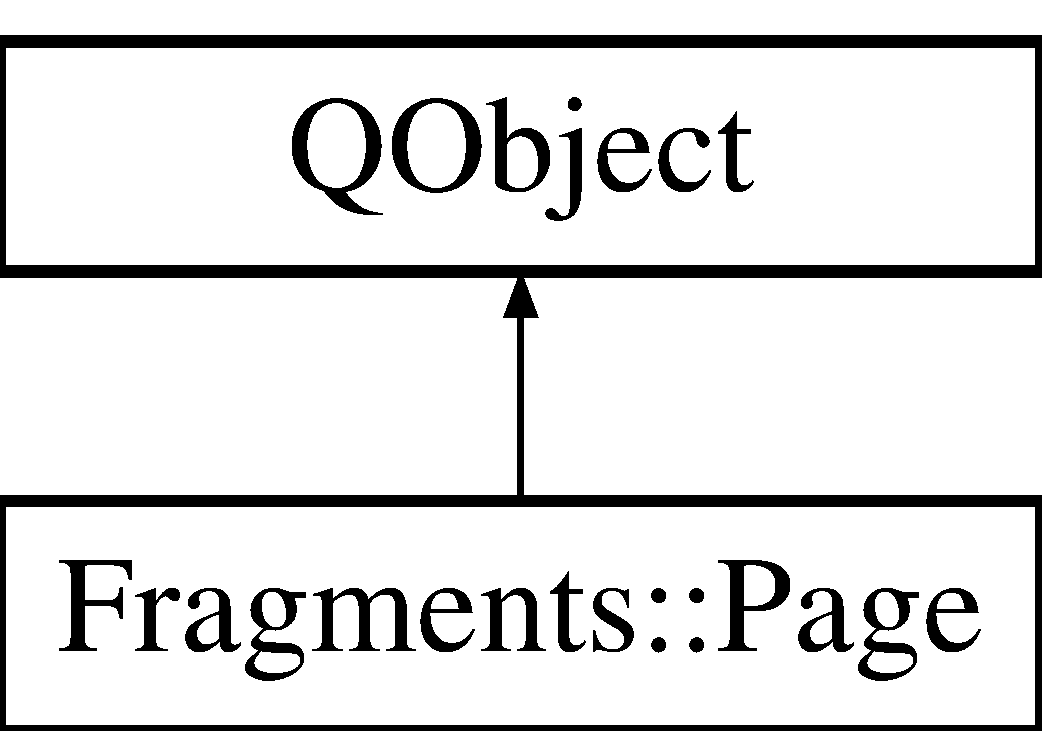
\includegraphics[height=2.000000cm]{classFragments_1_1Page}
\end{center}
\end{figure}
\subsection*{Signals}
\begin{DoxyCompactItemize}
\item 
\mbox{\Hypertarget{classFragments_1_1Page_a03f40d5c9520331432c9f1c7ab9f805c}\label{classFragments_1_1Page_a03f40d5c9520331432c9f1c7ab9f805c}} 
void {\bfseries uri\+Changed} ()
\item 
\mbox{\Hypertarget{classFragments_1_1Page_acfdd19abc8342361f975b4d9d10e2e64}\label{classFragments_1_1Page_acfdd19abc8342361f975b4d9d10e2e64}} 
void {\bfseries timestamp\+Changed} ()
\item 
\mbox{\Hypertarget{classFragments_1_1Page_a0b56ee63d18b43654cdfebd6a39c8d4f}\label{classFragments_1_1Page_a0b56ee63d18b43654cdfebd6a39c8d4f}} 
void {\bfseries hydra\+Next\+Changed} ()
\item 
\mbox{\Hypertarget{classFragments_1_1Page_a6f63a3428523cfa79ab30bfce32c0509}\label{classFragments_1_1Page_a6f63a3428523cfa79ab30bfce32c0509}} 
void {\bfseries hydra\+Previous\+Changed} ()
\item 
\mbox{\Hypertarget{classFragments_1_1Page_a6d449124d048af31d3e1e24a66c34636}\label{classFragments_1_1Page_a6d449124d048af31d3e1e24a66c34636}} 
void {\bfseries fragments\+Changed} ()
\end{DoxyCompactItemize}
\subsection*{Public Member Functions}
\begin{DoxyCompactItemize}
\item 
\mbox{\Hypertarget{classFragments_1_1Page_af61cfda59ee42caa75e373471ac91ae6}\label{classFragments_1_1Page_af61cfda59ee42caa75e373471ac91ae6}} 
{\bfseries Page} (Q\+Object $\ast$parent=nullptr)
\item 
\mbox{\Hypertarget{classFragments_1_1Page_ac345c0f46af8796c9f7fa702f71f240c}\label{classFragments_1_1Page_ac345c0f46af8796c9f7fa702f71f240c}} 
{\bfseries Page} (const Q\+Url \&uri, const Q\+Date\+Time \&timestamp, const Q\+Url \&hydra\+Next, const Q\+Url \&hydra\+Previous, const Q\+List$<$ \mbox{\hyperlink{classFragments_1_1Fragment}{Fragments\+::\+Fragment}} $\ast$$>$ \&fragments, Q\+Object $\ast$parent=nullptr)
\item 
\mbox{\Hypertarget{classFragments_1_1Page_a1185c1fb78c1d28eee03dba926fefcb8}\label{classFragments_1_1Page_a1185c1fb78c1d28eee03dba926fefcb8}} 
Q\+Url {\bfseries uri} () const
\item 
\mbox{\Hypertarget{classFragments_1_1Page_a13d34067ae20ee41b3003a6c2084fe2c}\label{classFragments_1_1Page_a13d34067ae20ee41b3003a6c2084fe2c}} 
void {\bfseries set\+U\+RI} (const Q\+Url \&uri)
\item 
\mbox{\Hypertarget{classFragments_1_1Page_a44cf4faf8776d3344bc4296d37b1f7ae}\label{classFragments_1_1Page_a44cf4faf8776d3344bc4296d37b1f7ae}} 
Q\+Date\+Time {\bfseries timestamp} () const
\item 
\mbox{\Hypertarget{classFragments_1_1Page_a5f771039432d7c46a7da56d34474bb8a}\label{classFragments_1_1Page_a5f771039432d7c46a7da56d34474bb8a}} 
void {\bfseries set\+Timestamp} (const Q\+Date\+Time \&timestamp)
\item 
\mbox{\Hypertarget{classFragments_1_1Page_a822bbc500bf1e5540582cdf258d73b20}\label{classFragments_1_1Page_a822bbc500bf1e5540582cdf258d73b20}} 
Q\+Url {\bfseries hydra\+Next} () const
\item 
\mbox{\Hypertarget{classFragments_1_1Page_a241195084d7c53ce0c8ad2fff67d9698}\label{classFragments_1_1Page_a241195084d7c53ce0c8ad2fff67d9698}} 
void {\bfseries set\+Hydra\+Next} (const Q\+Url \&hydra\+Next)
\item 
\mbox{\Hypertarget{classFragments_1_1Page_a102aada029299dbe7f8b55116eda0933}\label{classFragments_1_1Page_a102aada029299dbe7f8b55116eda0933}} 
Q\+Url {\bfseries hydra\+Previous} () const
\item 
\mbox{\Hypertarget{classFragments_1_1Page_a262f978bd4837db5e1c50b59a7984608}\label{classFragments_1_1Page_a262f978bd4837db5e1c50b59a7984608}} 
void {\bfseries set\+Hydra\+Previous} (const Q\+Url \&hydra\+Previous)
\item 
\mbox{\Hypertarget{classFragments_1_1Page_ab2460084209c3fe9211f70689ad78019}\label{classFragments_1_1Page_ab2460084209c3fe9211f70689ad78019}} 
Q\+List$<$ \mbox{\hyperlink{classFragments_1_1Fragment}{Fragments\+::\+Fragment}} $\ast$ $>$ {\bfseries fragments} () const
\item 
\mbox{\Hypertarget{classFragments_1_1Page_a41d271ad74d1aaf0b5de36d8619306f5}\label{classFragments_1_1Page_a41d271ad74d1aaf0b5de36d8619306f5}} 
void {\bfseries set\+Fragments} (const Q\+List$<$ \mbox{\hyperlink{classFragments_1_1Fragment}{Fragments\+::\+Fragment}} $\ast$$>$ \&fragments)
\end{DoxyCompactItemize}
\subsection*{Private Attributes}
\begin{DoxyCompactItemize}
\item 
\mbox{\Hypertarget{classFragments_1_1Page_ac674951355ab6c5e9c1aa7d8eeb7dbff}\label{classFragments_1_1Page_ac674951355ab6c5e9c1aa7d8eeb7dbff}} 
Q\+Url {\bfseries m\+\_\+uri}
\item 
\mbox{\Hypertarget{classFragments_1_1Page_a0bbe4f3dd97422b2e70936394fa755c6}\label{classFragments_1_1Page_a0bbe4f3dd97422b2e70936394fa755c6}} 
Q\+Date\+Time {\bfseries m\+\_\+timestamp}
\item 
\mbox{\Hypertarget{classFragments_1_1Page_aa6f58f42bfe8678444a170d1cbbe9902}\label{classFragments_1_1Page_aa6f58f42bfe8678444a170d1cbbe9902}} 
Q\+Url {\bfseries m\+\_\+hydra\+Next}
\item 
\mbox{\Hypertarget{classFragments_1_1Page_a3f6de09ddfb6d757b675f252c12bd4d8}\label{classFragments_1_1Page_a3f6de09ddfb6d757b675f252c12bd4d8}} 
Q\+Url {\bfseries m\+\_\+hydra\+Previous}
\item 
\mbox{\Hypertarget{classFragments_1_1Page_aac92876ae3e054b37430ee03b877d6b9}\label{classFragments_1_1Page_aac92876ae3e054b37430ee03b877d6b9}} 
Q\+List$<$ \mbox{\hyperlink{classFragments_1_1Fragment}{Fragments\+::\+Fragment}} $\ast$ $>$ {\bfseries m\+\_\+fragments}
\end{DoxyCompactItemize}


The documentation for this class was generated from the following files\+:\begin{DoxyCompactItemize}
\item 
src/include/fragments/fragmentspage.\+h\item 
src/fragments/\mbox{\hyperlink{fragmentspage_8cpp}{fragmentspage.\+cpp}}\end{DoxyCompactItemize}

\hypertarget{classCSA_1_1Planner}{}\section{C\+SA\+:\+:Planner Class Reference}
\label{classCSA_1_1Planner}\index{C\+S\+A\+::\+Planner@{C\+S\+A\+::\+Planner}}


{\ttfamily \#include $<$csaplanner.\+h$>$}

Inheritance diagram for C\+SA\+:\+:Planner\+:\begin{figure}[H]
\begin{center}
\leavevmode
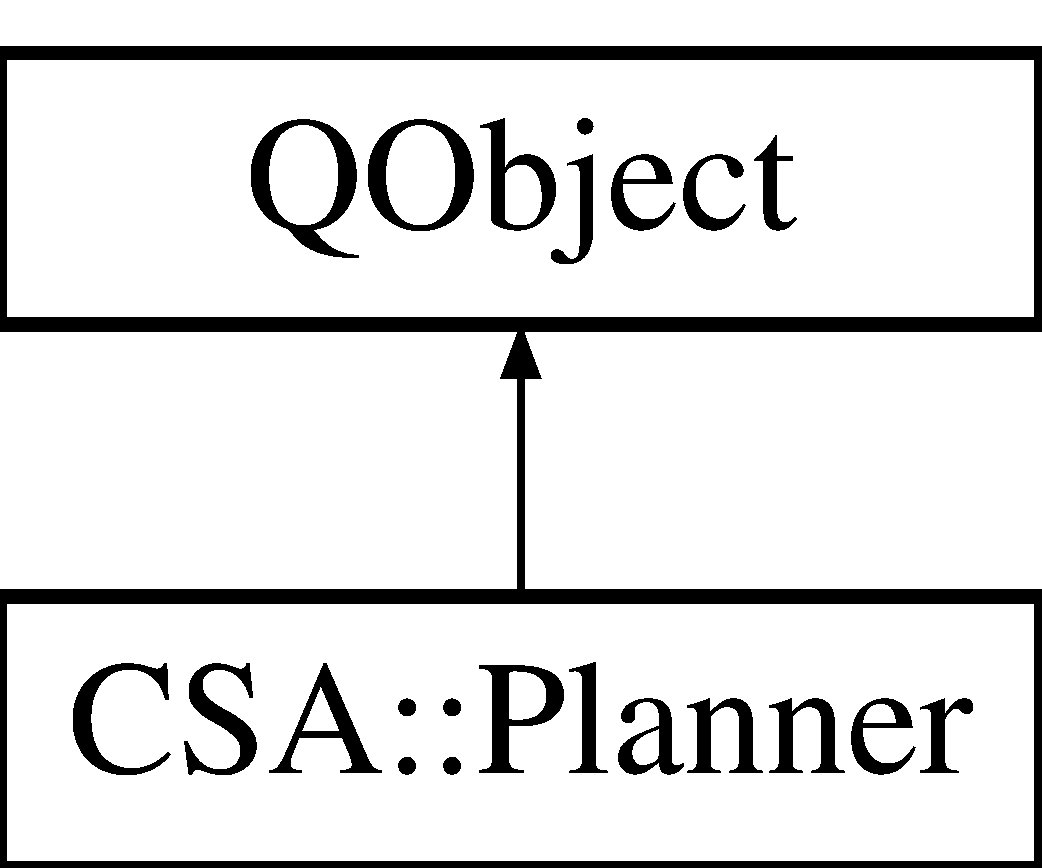
\includegraphics[height=2.000000cm]{classCSA_1_1Planner}
\end{center}
\end{figure}
\subsection*{Signals}
\begin{DoxyCompactItemize}
\item 
void \mbox{\hyperlink{classCSA_1_1Planner_aef9242efc2f34759d0bc58da60b10baf}{routes\+Found}} (const Q\+List$<$ \mbox{\hyperlink{classCSA_1_1Route}{C\+S\+A\+::\+Route}} $\ast$$>$ \&\mbox{\hyperlink{classCSA_1_1Planner_a1ecc41dc060aafd6e2ce0f2c4a52648b}{routes}})
\item 
void \mbox{\hyperlink{classCSA_1_1Planner_a4057e2f24927818deb1857c47a5008cf}{error}} (const Q\+String \&message)
\item 
void \mbox{\hyperlink{classCSA_1_1Planner_a54e3e7049b018f3cd08697e39149add3}{page\+Requested}} (const Q\+Url \&page\+U\+RI)
\item 
void \mbox{\hyperlink{classCSA_1_1Planner_af9fcdc9efcb27c4e45ddc36367a1364c}{page\+Received}} (const Q\+Url \&page\+U\+RI)
\item 
void \mbox{\hyperlink{classCSA_1_1Planner_a987cbbe8316beb1db2983ac62ccbed03}{page\+Progress}} (const Q\+Url \&page\+U\+RI, const qint16 \&progress)
\end{DoxyCompactItemize}
\subsection*{Public Member Functions}
\begin{DoxyCompactItemize}
\item 
void \mbox{\hyperlink{classCSA_1_1Planner_aebe12cc6eabe41e6e843ebab182d44ab}{get\+Connections}} (const Q\+Url \&departure\+Station, const Q\+Url \&arrival\+Station, const Q\+Date\+Time \&\mbox{\hyperlink{classCSA_1_1Planner_affe50069469ecc6b75c69efdb408b71a}{departure\+Time}}, const qint16 \&\mbox{\hyperlink{classCSA_1_1Planner_a2b734fc3d3ae3af744876bdc72898596}{max\+Transfers}})
\item 
Q\+Date\+Time \mbox{\hyperlink{classCSA_1_1Planner_a78671efec5a97e327b77bd2c9e03cf15}{calculate\+Arrival\+Time}} (const Q\+Date\+Time \&\mbox{\hyperlink{classCSA_1_1Planner_affe50069469ecc6b75c69efdb408b71a}{departure\+Time}})
\item 
Q\+Date\+Time \mbox{\hyperlink{classCSA_1_1Planner_affe50069469ecc6b75c69efdb408b71a}{departure\+Time}} () const
\item 
void \mbox{\hyperlink{classCSA_1_1Planner_ac97fdf7ce0d6b9a5f0d74e884927147c}{set\+Departure\+Time}} (const Q\+Date\+Time \&\mbox{\hyperlink{classCSA_1_1Planner_affe50069469ecc6b75c69efdb408b71a}{departure\+Time}})
\item 
Q\+Date\+Time \mbox{\hyperlink{classCSA_1_1Planner_a1ae3eafa8ebde74343828fa98cb588b7}{arrival\+Time}} () const
\item 
void \mbox{\hyperlink{classCSA_1_1Planner_a140baeba635ac0e6d794747aa594e17f}{set\+Arrival\+Time}} (const Q\+Date\+Time \&\mbox{\hyperlink{classCSA_1_1Planner_a1ae3eafa8ebde74343828fa98cb588b7}{arrival\+Time}})
\item 
qint16 \mbox{\hyperlink{classCSA_1_1Planner_a2b734fc3d3ae3af744876bdc72898596}{max\+Transfers}} () const
\item 
void \mbox{\hyperlink{classCSA_1_1Planner_a950c1dc8208d98aab977f490c2e7b244}{set\+Max\+Transfers}} (const qint16 \&\mbox{\hyperlink{classCSA_1_1Planner_a2b734fc3d3ae3af744876bdc72898596}{max\+Transfers}})
\item 
Q\+Url \mbox{\hyperlink{classCSA_1_1Planner_a3b84dde21b6abaf92014af54b1cd7fe8}{departure\+Station\+U\+RI}} () const
\item 
void \mbox{\hyperlink{classCSA_1_1Planner_a562537d6903362f084d8aa08f812d441}{set\+Departure\+Station\+U\+RI}} (const Q\+Url \&\mbox{\hyperlink{classCSA_1_1Planner_a3b84dde21b6abaf92014af54b1cd7fe8}{departure\+Station\+U\+RI}})
\item 
Q\+Url \mbox{\hyperlink{classCSA_1_1Planner_ac412f34346e0bdd24d62b06d8770b150}{arrival\+Station\+U\+RI}} () const
\item 
void \mbox{\hyperlink{classCSA_1_1Planner_aab52e8e5b484f773a33923fd3f29be25}{set\+Arrival\+Station\+U\+RI}} (const Q\+Url \&\mbox{\hyperlink{classCSA_1_1Planner_ac412f34346e0bdd24d62b06d8770b150}{arrival\+Station\+U\+RI}})
\end{DoxyCompactItemize}
\subsection*{Static Public Member Functions}
\begin{DoxyCompactItemize}
\item 
static \mbox{\hyperlink{classCSA_1_1Planner}{Planner}} $\ast$ \mbox{\hyperlink{classCSA_1_1Planner_a0a361e4991bc8f1f29b41507c13ea590}{get\+Instance}} (Q\+Object $\ast$parent=nullptr)
\end{DoxyCompactItemize}
\subsection*{Private Slots}
\begin{DoxyCompactItemize}
\item 
void \mbox{\hyperlink{classCSA_1_1Planner_ac1b6ffca527db0fe0ff6f904b6a0ee35}{page\+Received}} (\mbox{\hyperlink{classFragments_1_1Page}{Fragments\+::\+Page}} $\ast$page)
\end{DoxyCompactItemize}
\subsection*{Private Member Functions}
\begin{DoxyCompactItemize}
\item 
\mbox{\hyperlink{classCSA_1_1Planner_aa0015d0596c5b78bf29f65276fcc8852}{Planner}} (Q\+Object $\ast$parent)
\item 
void \mbox{\hyperlink{classCSA_1_1Planner_a2539dd808dc988ef5cb0b4b7f4de0077}{plan\+Page}} (\mbox{\hyperlink{classFragments_1_1Page}{Fragments\+::\+Page}} $\ast$page)
\item 
\mbox{\hyperlink{classCSA_1_1StationStopProfile}{Station\+Stop\+Profile}} $\ast$ \mbox{\hyperlink{classCSA_1_1Planner_a68af05f5dc3eaa5d204224c21c80f42d}{get\+First\+Reachable\+Connection}} (\mbox{\hyperlink{classCSA_1_1StationStopProfile}{Station\+Stop\+Profile}} $\ast$arrival\+Profile)
\item 
\mbox{\hyperlink{classFragments_1_1Factory}{Fragments\+::\+Factory}} $\ast$ \mbox{\hyperlink{classCSA_1_1Planner_a7395c140e3cd577ed459350d4e5588ad}{Factory}} () const
\item 
void \mbox{\hyperlink{classCSA_1_1Planner_a6f6fe97b8620230960514f544109f076}{set\+Factory}} (\mbox{\hyperlink{classFragments_1_1Factory}{Fragments\+::\+Factory}} $\ast$value)
\item 
\mbox{\hyperlink{classCSA_1_1StationFactory}{C\+S\+A\+::\+Station\+Factory}} $\ast$ \mbox{\hyperlink{classCSA_1_1Planner_aa6f6d8a3714aa2846f19a41da4f1959b}{station\+Factory}} () const
\item 
void \mbox{\hyperlink{classCSA_1_1Planner_a67b39227b11c5d49052c48141ad256ac}{set\+Station\+Factory}} (\mbox{\hyperlink{classCSA_1_1StationFactory}{C\+S\+A\+::\+Station\+Factory}} $\ast$\mbox{\hyperlink{classCSA_1_1Planner_aa6f6d8a3714aa2846f19a41da4f1959b}{station\+Factory}})
\item 
Q\+List$<$ \mbox{\hyperlink{classCSA_1_1Route}{C\+S\+A\+::\+Route}} $\ast$ $>$ \mbox{\hyperlink{classCSA_1_1Planner_a1ecc41dc060aafd6e2ce0f2c4a52648b}{routes}} () const
\item 
void \mbox{\hyperlink{classCSA_1_1Planner_a596d6e4038e76ff4944cab418594858f}{set\+Routes}} (const Q\+List$<$ \mbox{\hyperlink{classCSA_1_1Route}{C\+S\+A\+::\+Route}} $\ast$$>$ \&\mbox{\hyperlink{classCSA_1_1Planner_a1ecc41dc060aafd6e2ce0f2c4a52648b}{routes}})
\item 
Q\+Map$<$ Q\+Url, Q\+List$<$ \mbox{\hyperlink{classCSA_1_1StationStopProfile}{C\+S\+A\+::\+Station\+Stop\+Profile}} $\ast$ $>$ $>$ \mbox{\hyperlink{classCSA_1_1Planner_af8b23db7e72d8bf8d7a219d569c853c6}{S\+Array}} () const
\item 
void \mbox{\hyperlink{classCSA_1_1Planner_af19efcec5cc9196698108f30fa55029c}{set\+S\+Array}} (const Q\+Map$<$ Q\+Url, Q\+List$<$ \mbox{\hyperlink{classCSA_1_1StationStopProfile}{C\+S\+A\+::\+Station\+Stop\+Profile}} $\ast$$>$ $>$ \&\mbox{\hyperlink{classCSA_1_1Planner_af8b23db7e72d8bf8d7a219d569c853c6}{S\+Array}})
\item 
Q\+Map$<$ Q\+Url, \mbox{\hyperlink{classCSA_1_1TrainProfile}{C\+S\+A\+::\+Train\+Profile}} $\ast$ $>$ \mbox{\hyperlink{classCSA_1_1Planner_a0e8ccca51c26f77086bddaf28ec521a2}{T\+Array}} () const
\item 
void \mbox{\hyperlink{classCSA_1_1Planner_a376be1acb09685a367131b290af81910}{set\+T\+Array}} (const Q\+Map$<$ Q\+Url, \mbox{\hyperlink{classCSA_1_1TrainProfile}{C\+S\+A\+::\+Train\+Profile}} $\ast$$>$ \&\mbox{\hyperlink{classCSA_1_1Planner_a0e8ccca51c26f77086bddaf28ec521a2}{T\+Array}})
\end{DoxyCompactItemize}
\subsection*{Private Attributes}
\begin{DoxyCompactItemize}
\item 
Q\+Mutex \mbox{\hyperlink{classCSA_1_1Planner_adfeb70ddbedfbb37567b852aa7b8cbe3}{sync\+Thread\+Mutex}}
\item 
\mbox{\hyperlink{classFragments_1_1Factory}{Fragments\+::\+Factory}} $\ast$ \mbox{\hyperlink{classCSA_1_1Planner_a125612862843283f437f76dbc2ae56ba}{m\+\_\+linked\+Connection\+Factory}}
\item 
\mbox{\hyperlink{classCSA_1_1StationFactory}{C\+S\+A\+::\+Station\+Factory}} $\ast$ \mbox{\hyperlink{classCSA_1_1Planner_a14aa8633412e69b1b26624ae4a63a478}{m\+\_\+station\+Factory}}
\item 
Q\+Url \mbox{\hyperlink{classCSA_1_1Planner_aa5eb52a86c4d14053de75f4b293409fa}{m\+\_\+departure\+Station\+U\+RI}}
\item 
Q\+Url \mbox{\hyperlink{classCSA_1_1Planner_a8f0231d1da5fc7451ef9127970ec3ff1}{m\+\_\+arrival\+Station\+U\+RI}}
\item 
Q\+Date\+Time \mbox{\hyperlink{classCSA_1_1Planner_a79f5a12513524607b1fbbdcf9bd4162d}{m\+\_\+departure\+Time}}
\item 
Q\+Date\+Time \mbox{\hyperlink{classCSA_1_1Planner_a96a9ae70c8919e65e81cd095355a7ea0}{m\+\_\+arrival\+Time}}
\item 
qint16 \mbox{\hyperlink{classCSA_1_1Planner_a4b24326fa4784c61865526532935cd97}{m\+\_\+max\+Transfers}}
\item 
Q\+List$<$ \mbox{\hyperlink{classCSA_1_1Route}{C\+S\+A\+::\+Route}} $\ast$ $>$ \mbox{\hyperlink{classCSA_1_1Planner_af978da0a218f6eecf870e8f4a3d6d294}{m\+\_\+routes}}
\item 
Q\+Map$<$ Q\+Url, Q\+List$<$ \mbox{\hyperlink{classCSA_1_1StationStopProfile}{C\+S\+A\+::\+Station\+Stop\+Profile}} $\ast$ $>$ $>$ \mbox{\hyperlink{classCSA_1_1Planner_adfc501aa7ae4f55c3fab20890e6bb980}{m\+\_\+\+S\+Array}}
\item 
Q\+Map$<$ Q\+Url, \mbox{\hyperlink{classCSA_1_1TrainProfile}{C\+S\+A\+::\+Train\+Profile}} $\ast$ $>$ \mbox{\hyperlink{classCSA_1_1Planner_a9787a967e79e8efb703bdf5e2e5718c7}{m\+\_\+\+T\+Array}}
\end{DoxyCompactItemize}
\subsection*{Static Private Attributes}
\begin{DoxyCompactItemize}
\item 
static \mbox{\hyperlink{classCSA_1_1Planner}{C\+S\+A\+::\+Planner}} $\ast$ \mbox{\hyperlink{classCSA_1_1Planner_a85076417b9aca86ba069c447e3ecdaa0}{m\+\_\+instance}} = nullptr
\end{DoxyCompactItemize}


\subsection{Constructor \& Destructor Documentation}
\mbox{\Hypertarget{classCSA_1_1Planner_aa0015d0596c5b78bf29f65276fcc8852}\label{classCSA_1_1Planner_aa0015d0596c5b78bf29f65276fcc8852}} 
\index{C\+S\+A\+::\+Planner@{C\+S\+A\+::\+Planner}!Planner@{Planner}}
\index{Planner@{Planner}!C\+S\+A\+::\+Planner@{C\+S\+A\+::\+Planner}}
\subsubsection{\texorpdfstring{Planner()}{Planner()}}
{\footnotesize\ttfamily C\+S\+A\+::\+Planner\+::\+Planner (\begin{DoxyParamCaption}\item[{Q\+Object $\ast$}]{parent }\end{DoxyParamCaption})\hspace{0.3cm}{\ttfamily [explicit]}, {\ttfamily [private]}}



\subsection{Member Function Documentation}
\mbox{\Hypertarget{classCSA_1_1Planner_ac412f34346e0bdd24d62b06d8770b150}\label{classCSA_1_1Planner_ac412f34346e0bdd24d62b06d8770b150}} 
\index{C\+S\+A\+::\+Planner@{C\+S\+A\+::\+Planner}!arrival\+Station\+U\+RI@{arrival\+Station\+U\+RI}}
\index{arrival\+Station\+U\+RI@{arrival\+Station\+U\+RI}!C\+S\+A\+::\+Planner@{C\+S\+A\+::\+Planner}}
\subsubsection{\texorpdfstring{arrival\+Station\+U\+R\+I()}{arrivalStationURI()}}
{\footnotesize\ttfamily Q\+Url C\+S\+A\+::\+Planner\+::arrival\+Station\+U\+RI (\begin{DoxyParamCaption}{ }\end{DoxyParamCaption}) const}

\mbox{\Hypertarget{classCSA_1_1Planner_a1ae3eafa8ebde74343828fa98cb588b7}\label{classCSA_1_1Planner_a1ae3eafa8ebde74343828fa98cb588b7}} 
\index{C\+S\+A\+::\+Planner@{C\+S\+A\+::\+Planner}!arrival\+Time@{arrival\+Time}}
\index{arrival\+Time@{arrival\+Time}!C\+S\+A\+::\+Planner@{C\+S\+A\+::\+Planner}}
\subsubsection{\texorpdfstring{arrival\+Time()}{arrivalTime()}}
{\footnotesize\ttfamily Q\+Date\+Time C\+S\+A\+::\+Planner\+::arrival\+Time (\begin{DoxyParamCaption}{ }\end{DoxyParamCaption}) const}

\mbox{\Hypertarget{classCSA_1_1Planner_a78671efec5a97e327b77bd2c9e03cf15}\label{classCSA_1_1Planner_a78671efec5a97e327b77bd2c9e03cf15}} 
\index{C\+S\+A\+::\+Planner@{C\+S\+A\+::\+Planner}!calculate\+Arrival\+Time@{calculate\+Arrival\+Time}}
\index{calculate\+Arrival\+Time@{calculate\+Arrival\+Time}!C\+S\+A\+::\+Planner@{C\+S\+A\+::\+Planner}}
\subsubsection{\texorpdfstring{calculate\+Arrival\+Time()}{calculateArrivalTime()}}
{\footnotesize\ttfamily Q\+Date\+Time C\+S\+A\+::\+Planner\+::calculate\+Arrival\+Time (\begin{DoxyParamCaption}\item[{const Q\+Date\+Time \&}]{departure\+Time }\end{DoxyParamCaption})}

\mbox{\Hypertarget{classCSA_1_1Planner_a3b84dde21b6abaf92014af54b1cd7fe8}\label{classCSA_1_1Planner_a3b84dde21b6abaf92014af54b1cd7fe8}} 
\index{C\+S\+A\+::\+Planner@{C\+S\+A\+::\+Planner}!departure\+Station\+U\+RI@{departure\+Station\+U\+RI}}
\index{departure\+Station\+U\+RI@{departure\+Station\+U\+RI}!C\+S\+A\+::\+Planner@{C\+S\+A\+::\+Planner}}
\subsubsection{\texorpdfstring{departure\+Station\+U\+R\+I()}{departureStationURI()}}
{\footnotesize\ttfamily Q\+Url C\+S\+A\+::\+Planner\+::departure\+Station\+U\+RI (\begin{DoxyParamCaption}{ }\end{DoxyParamCaption}) const}

\mbox{\Hypertarget{classCSA_1_1Planner_affe50069469ecc6b75c69efdb408b71a}\label{classCSA_1_1Planner_affe50069469ecc6b75c69efdb408b71a}} 
\index{C\+S\+A\+::\+Planner@{C\+S\+A\+::\+Planner}!departure\+Time@{departure\+Time}}
\index{departure\+Time@{departure\+Time}!C\+S\+A\+::\+Planner@{C\+S\+A\+::\+Planner}}
\subsubsection{\texorpdfstring{departure\+Time()}{departureTime()}}
{\footnotesize\ttfamily Q\+Date\+Time C\+S\+A\+::\+Planner\+::departure\+Time (\begin{DoxyParamCaption}{ }\end{DoxyParamCaption}) const}

\mbox{\Hypertarget{classCSA_1_1Planner_a4057e2f24927818deb1857c47a5008cf}\label{classCSA_1_1Planner_a4057e2f24927818deb1857c47a5008cf}} 
\index{C\+S\+A\+::\+Planner@{C\+S\+A\+::\+Planner}!error@{error}}
\index{error@{error}!C\+S\+A\+::\+Planner@{C\+S\+A\+::\+Planner}}
\subsubsection{\texorpdfstring{error}{error}}
{\footnotesize\ttfamily void C\+S\+A\+::\+Planner\+::error (\begin{DoxyParamCaption}\item[{const Q\+String \&}]{message }\end{DoxyParamCaption})\hspace{0.3cm}{\ttfamily [signal]}}

\mbox{\Hypertarget{classCSA_1_1Planner_a7395c140e3cd577ed459350d4e5588ad}\label{classCSA_1_1Planner_a7395c140e3cd577ed459350d4e5588ad}} 
\index{C\+S\+A\+::\+Planner@{C\+S\+A\+::\+Planner}!Factory@{Factory}}
\index{Factory@{Factory}!C\+S\+A\+::\+Planner@{C\+S\+A\+::\+Planner}}
\subsubsection{\texorpdfstring{Factory()}{Factory()}}
{\footnotesize\ttfamily \mbox{\hyperlink{classFragments_1_1Factory}{Fragments\+::\+Factory}} $\ast$ C\+S\+A\+::\+Planner\+::\+Factory (\begin{DoxyParamCaption}{ }\end{DoxyParamCaption}) const\hspace{0.3cm}{\ttfamily [private]}}

\mbox{\Hypertarget{classCSA_1_1Planner_aebe12cc6eabe41e6e843ebab182d44ab}\label{classCSA_1_1Planner_aebe12cc6eabe41e6e843ebab182d44ab}} 
\index{C\+S\+A\+::\+Planner@{C\+S\+A\+::\+Planner}!get\+Connections@{get\+Connections}}
\index{get\+Connections@{get\+Connections}!C\+S\+A\+::\+Planner@{C\+S\+A\+::\+Planner}}
\subsubsection{\texorpdfstring{get\+Connections()}{getConnections()}}
{\footnotesize\ttfamily void C\+S\+A\+::\+Planner\+::get\+Connections (\begin{DoxyParamCaption}\item[{const Q\+Url \&}]{departure\+Station,  }\item[{const Q\+Url \&}]{arrival\+Station,  }\item[{const Q\+Date\+Time \&}]{departure\+Time,  }\item[{const qint16 \&}]{max\+Transfers }\end{DoxyParamCaption})}

\mbox{\Hypertarget{classCSA_1_1Planner_a68af05f5dc3eaa5d204224c21c80f42d}\label{classCSA_1_1Planner_a68af05f5dc3eaa5d204224c21c80f42d}} 
\index{C\+S\+A\+::\+Planner@{C\+S\+A\+::\+Planner}!get\+First\+Reachable\+Connection@{get\+First\+Reachable\+Connection}}
\index{get\+First\+Reachable\+Connection@{get\+First\+Reachable\+Connection}!C\+S\+A\+::\+Planner@{C\+S\+A\+::\+Planner}}
\subsubsection{\texorpdfstring{get\+First\+Reachable\+Connection()}{getFirstReachableConnection()}}
{\footnotesize\ttfamily \mbox{\hyperlink{classCSA_1_1StationStopProfile}{C\+S\+A\+::\+Station\+Stop\+Profile}} $\ast$ C\+S\+A\+::\+Planner\+::get\+First\+Reachable\+Connection (\begin{DoxyParamCaption}\item[{\mbox{\hyperlink{classCSA_1_1StationStopProfile}{C\+S\+A\+::\+Station\+Stop\+Profile}} $\ast$}]{arrival\+Profile }\end{DoxyParamCaption})\hspace{0.3cm}{\ttfamily [private]}}

\mbox{\Hypertarget{classCSA_1_1Planner_a0a361e4991bc8f1f29b41507c13ea590}\label{classCSA_1_1Planner_a0a361e4991bc8f1f29b41507c13ea590}} 
\index{C\+S\+A\+::\+Planner@{C\+S\+A\+::\+Planner}!get\+Instance@{get\+Instance}}
\index{get\+Instance@{get\+Instance}!C\+S\+A\+::\+Planner@{C\+S\+A\+::\+Planner}}
\subsubsection{\texorpdfstring{get\+Instance()}{getInstance()}}
{\footnotesize\ttfamily \mbox{\hyperlink{classCSA_1_1Planner}{C\+S\+A\+::\+Planner}} $\ast$ C\+S\+A\+::\+Planner\+::get\+Instance (\begin{DoxyParamCaption}\item[{Q\+Object $\ast$}]{parent = {\ttfamily nullptr} }\end{DoxyParamCaption})\hspace{0.3cm}{\ttfamily [static]}}

\mbox{\Hypertarget{classCSA_1_1Planner_a2b734fc3d3ae3af744876bdc72898596}\label{classCSA_1_1Planner_a2b734fc3d3ae3af744876bdc72898596}} 
\index{C\+S\+A\+::\+Planner@{C\+S\+A\+::\+Planner}!max\+Transfers@{max\+Transfers}}
\index{max\+Transfers@{max\+Transfers}!C\+S\+A\+::\+Planner@{C\+S\+A\+::\+Planner}}
\subsubsection{\texorpdfstring{max\+Transfers()}{maxTransfers()}}
{\footnotesize\ttfamily qint16 C\+S\+A\+::\+Planner\+::max\+Transfers (\begin{DoxyParamCaption}{ }\end{DoxyParamCaption}) const}

\mbox{\Hypertarget{classCSA_1_1Planner_a987cbbe8316beb1db2983ac62ccbed03}\label{classCSA_1_1Planner_a987cbbe8316beb1db2983ac62ccbed03}} 
\index{C\+S\+A\+::\+Planner@{C\+S\+A\+::\+Planner}!page\+Progress@{page\+Progress}}
\index{page\+Progress@{page\+Progress}!C\+S\+A\+::\+Planner@{C\+S\+A\+::\+Planner}}
\subsubsection{\texorpdfstring{page\+Progress}{pageProgress}}
{\footnotesize\ttfamily void C\+S\+A\+::\+Planner\+::page\+Progress (\begin{DoxyParamCaption}\item[{const Q\+Url \&}]{page\+U\+RI,  }\item[{const qint16 \&}]{progress }\end{DoxyParamCaption})\hspace{0.3cm}{\ttfamily [signal]}}

\mbox{\Hypertarget{classCSA_1_1Planner_af9fcdc9efcb27c4e45ddc36367a1364c}\label{classCSA_1_1Planner_af9fcdc9efcb27c4e45ddc36367a1364c}} 
\index{C\+S\+A\+::\+Planner@{C\+S\+A\+::\+Planner}!page\+Received@{page\+Received}}
\index{page\+Received@{page\+Received}!C\+S\+A\+::\+Planner@{C\+S\+A\+::\+Planner}}
\subsubsection{\texorpdfstring{page\+Received}{pageReceived}\hspace{0.1cm}{\footnotesize\ttfamily [1/2]}}
{\footnotesize\ttfamily void C\+S\+A\+::\+Planner\+::page\+Received (\begin{DoxyParamCaption}\item[{const Q\+Url \&}]{page\+U\+RI }\end{DoxyParamCaption})\hspace{0.3cm}{\ttfamily [signal]}}

\mbox{\Hypertarget{classCSA_1_1Planner_ac1b6ffca527db0fe0ff6f904b6a0ee35}\label{classCSA_1_1Planner_ac1b6ffca527db0fe0ff6f904b6a0ee35}} 
\index{C\+S\+A\+::\+Planner@{C\+S\+A\+::\+Planner}!page\+Received@{page\+Received}}
\index{page\+Received@{page\+Received}!C\+S\+A\+::\+Planner@{C\+S\+A\+::\+Planner}}
\subsubsection{\texorpdfstring{page\+Received}{pageReceived}\hspace{0.1cm}{\footnotesize\ttfamily [2/2]}}
{\footnotesize\ttfamily void C\+S\+A\+::\+Planner\+::page\+Received (\begin{DoxyParamCaption}\item[{\mbox{\hyperlink{classFragments_1_1Page}{Fragments\+::\+Page}} $\ast$}]{page }\end{DoxyParamCaption})\hspace{0.3cm}{\ttfamily [private]}, {\ttfamily [slot]}}

\mbox{\Hypertarget{classCSA_1_1Planner_a54e3e7049b018f3cd08697e39149add3}\label{classCSA_1_1Planner_a54e3e7049b018f3cd08697e39149add3}} 
\index{C\+S\+A\+::\+Planner@{C\+S\+A\+::\+Planner}!page\+Requested@{page\+Requested}}
\index{page\+Requested@{page\+Requested}!C\+S\+A\+::\+Planner@{C\+S\+A\+::\+Planner}}
\subsubsection{\texorpdfstring{page\+Requested}{pageRequested}}
{\footnotesize\ttfamily void C\+S\+A\+::\+Planner\+::page\+Requested (\begin{DoxyParamCaption}\item[{const Q\+Url \&}]{page\+U\+RI }\end{DoxyParamCaption})\hspace{0.3cm}{\ttfamily [signal]}}

\mbox{\Hypertarget{classCSA_1_1Planner_a2539dd808dc988ef5cb0b4b7f4de0077}\label{classCSA_1_1Planner_a2539dd808dc988ef5cb0b4b7f4de0077}} 
\index{C\+S\+A\+::\+Planner@{C\+S\+A\+::\+Planner}!plan\+Page@{plan\+Page}}
\index{plan\+Page@{plan\+Page}!C\+S\+A\+::\+Planner@{C\+S\+A\+::\+Planner}}
\subsubsection{\texorpdfstring{plan\+Page()}{planPage()}}
{\footnotesize\ttfamily void C\+S\+A\+::\+Planner\+::plan\+Page (\begin{DoxyParamCaption}\item[{\mbox{\hyperlink{classFragments_1_1Page}{Fragments\+::\+Page}} $\ast$}]{page }\end{DoxyParamCaption})\hspace{0.3cm}{\ttfamily [private]}}

\mbox{\Hypertarget{classCSA_1_1Planner_a1ecc41dc060aafd6e2ce0f2c4a52648b}\label{classCSA_1_1Planner_a1ecc41dc060aafd6e2ce0f2c4a52648b}} 
\index{C\+S\+A\+::\+Planner@{C\+S\+A\+::\+Planner}!routes@{routes}}
\index{routes@{routes}!C\+S\+A\+::\+Planner@{C\+S\+A\+::\+Planner}}
\subsubsection{\texorpdfstring{routes()}{routes()}}
{\footnotesize\ttfamily Q\+List$<$ \mbox{\hyperlink{classCSA_1_1Route}{C\+S\+A\+::\+Route}} $\ast$ $>$ C\+S\+A\+::\+Planner\+::routes (\begin{DoxyParamCaption}{ }\end{DoxyParamCaption}) const\hspace{0.3cm}{\ttfamily [private]}}

\mbox{\Hypertarget{classCSA_1_1Planner_aef9242efc2f34759d0bc58da60b10baf}\label{classCSA_1_1Planner_aef9242efc2f34759d0bc58da60b10baf}} 
\index{C\+S\+A\+::\+Planner@{C\+S\+A\+::\+Planner}!routes\+Found@{routes\+Found}}
\index{routes\+Found@{routes\+Found}!C\+S\+A\+::\+Planner@{C\+S\+A\+::\+Planner}}
\subsubsection{\texorpdfstring{routes\+Found}{routesFound}}
{\footnotesize\ttfamily void C\+S\+A\+::\+Planner\+::routes\+Found (\begin{DoxyParamCaption}\item[{const Q\+List$<$ \mbox{\hyperlink{classCSA_1_1Route}{C\+S\+A\+::\+Route}} $\ast$$>$ \&}]{routes }\end{DoxyParamCaption})\hspace{0.3cm}{\ttfamily [signal]}}

\mbox{\Hypertarget{classCSA_1_1Planner_af8b23db7e72d8bf8d7a219d569c853c6}\label{classCSA_1_1Planner_af8b23db7e72d8bf8d7a219d569c853c6}} 
\index{C\+S\+A\+::\+Planner@{C\+S\+A\+::\+Planner}!S\+Array@{S\+Array}}
\index{S\+Array@{S\+Array}!C\+S\+A\+::\+Planner@{C\+S\+A\+::\+Planner}}
\subsubsection{\texorpdfstring{S\+Array()}{SArray()}}
{\footnotesize\ttfamily Q\+Map$<$ Q\+Url, Q\+List$<$ \mbox{\hyperlink{classCSA_1_1StationStopProfile}{C\+S\+A\+::\+Station\+Stop\+Profile}} $\ast$ $>$ $>$ C\+S\+A\+::\+Planner\+::\+S\+Array (\begin{DoxyParamCaption}{ }\end{DoxyParamCaption}) const\hspace{0.3cm}{\ttfamily [private]}}

\mbox{\Hypertarget{classCSA_1_1Planner_aab52e8e5b484f773a33923fd3f29be25}\label{classCSA_1_1Planner_aab52e8e5b484f773a33923fd3f29be25}} 
\index{C\+S\+A\+::\+Planner@{C\+S\+A\+::\+Planner}!set\+Arrival\+Station\+U\+RI@{set\+Arrival\+Station\+U\+RI}}
\index{set\+Arrival\+Station\+U\+RI@{set\+Arrival\+Station\+U\+RI}!C\+S\+A\+::\+Planner@{C\+S\+A\+::\+Planner}}
\subsubsection{\texorpdfstring{set\+Arrival\+Station\+U\+R\+I()}{setArrivalStationURI()}}
{\footnotesize\ttfamily void C\+S\+A\+::\+Planner\+::set\+Arrival\+Station\+U\+RI (\begin{DoxyParamCaption}\item[{const Q\+Url \&}]{arrival\+Station\+U\+RI }\end{DoxyParamCaption})}

\mbox{\Hypertarget{classCSA_1_1Planner_a140baeba635ac0e6d794747aa594e17f}\label{classCSA_1_1Planner_a140baeba635ac0e6d794747aa594e17f}} 
\index{C\+S\+A\+::\+Planner@{C\+S\+A\+::\+Planner}!set\+Arrival\+Time@{set\+Arrival\+Time}}
\index{set\+Arrival\+Time@{set\+Arrival\+Time}!C\+S\+A\+::\+Planner@{C\+S\+A\+::\+Planner}}
\subsubsection{\texorpdfstring{set\+Arrival\+Time()}{setArrivalTime()}}
{\footnotesize\ttfamily void C\+S\+A\+::\+Planner\+::set\+Arrival\+Time (\begin{DoxyParamCaption}\item[{const Q\+Date\+Time \&}]{arrival\+Time }\end{DoxyParamCaption})}

\mbox{\Hypertarget{classCSA_1_1Planner_a562537d6903362f084d8aa08f812d441}\label{classCSA_1_1Planner_a562537d6903362f084d8aa08f812d441}} 
\index{C\+S\+A\+::\+Planner@{C\+S\+A\+::\+Planner}!set\+Departure\+Station\+U\+RI@{set\+Departure\+Station\+U\+RI}}
\index{set\+Departure\+Station\+U\+RI@{set\+Departure\+Station\+U\+RI}!C\+S\+A\+::\+Planner@{C\+S\+A\+::\+Planner}}
\subsubsection{\texorpdfstring{set\+Departure\+Station\+U\+R\+I()}{setDepartureStationURI()}}
{\footnotesize\ttfamily void C\+S\+A\+::\+Planner\+::set\+Departure\+Station\+U\+RI (\begin{DoxyParamCaption}\item[{const Q\+Url \&}]{departure\+Station\+U\+RI }\end{DoxyParamCaption})}

\mbox{\Hypertarget{classCSA_1_1Planner_ac97fdf7ce0d6b9a5f0d74e884927147c}\label{classCSA_1_1Planner_ac97fdf7ce0d6b9a5f0d74e884927147c}} 
\index{C\+S\+A\+::\+Planner@{C\+S\+A\+::\+Planner}!set\+Departure\+Time@{set\+Departure\+Time}}
\index{set\+Departure\+Time@{set\+Departure\+Time}!C\+S\+A\+::\+Planner@{C\+S\+A\+::\+Planner}}
\subsubsection{\texorpdfstring{set\+Departure\+Time()}{setDepartureTime()}}
{\footnotesize\ttfamily void C\+S\+A\+::\+Planner\+::set\+Departure\+Time (\begin{DoxyParamCaption}\item[{const Q\+Date\+Time \&}]{departure\+Time }\end{DoxyParamCaption})}

\mbox{\Hypertarget{classCSA_1_1Planner_a6f6fe97b8620230960514f544109f076}\label{classCSA_1_1Planner_a6f6fe97b8620230960514f544109f076}} 
\index{C\+S\+A\+::\+Planner@{C\+S\+A\+::\+Planner}!set\+Factory@{set\+Factory}}
\index{set\+Factory@{set\+Factory}!C\+S\+A\+::\+Planner@{C\+S\+A\+::\+Planner}}
\subsubsection{\texorpdfstring{set\+Factory()}{setFactory()}}
{\footnotesize\ttfamily void C\+S\+A\+::\+Planner\+::set\+Factory (\begin{DoxyParamCaption}\item[{\mbox{\hyperlink{classFragments_1_1Factory}{Fragments\+::\+Factory}} $\ast$}]{value }\end{DoxyParamCaption})\hspace{0.3cm}{\ttfamily [private]}}

\mbox{\Hypertarget{classCSA_1_1Planner_a950c1dc8208d98aab977f490c2e7b244}\label{classCSA_1_1Planner_a950c1dc8208d98aab977f490c2e7b244}} 
\index{C\+S\+A\+::\+Planner@{C\+S\+A\+::\+Planner}!set\+Max\+Transfers@{set\+Max\+Transfers}}
\index{set\+Max\+Transfers@{set\+Max\+Transfers}!C\+S\+A\+::\+Planner@{C\+S\+A\+::\+Planner}}
\subsubsection{\texorpdfstring{set\+Max\+Transfers()}{setMaxTransfers()}}
{\footnotesize\ttfamily void C\+S\+A\+::\+Planner\+::set\+Max\+Transfers (\begin{DoxyParamCaption}\item[{const qint16 \&}]{max\+Transfers }\end{DoxyParamCaption})}

\mbox{\Hypertarget{classCSA_1_1Planner_a596d6e4038e76ff4944cab418594858f}\label{classCSA_1_1Planner_a596d6e4038e76ff4944cab418594858f}} 
\index{C\+S\+A\+::\+Planner@{C\+S\+A\+::\+Planner}!set\+Routes@{set\+Routes}}
\index{set\+Routes@{set\+Routes}!C\+S\+A\+::\+Planner@{C\+S\+A\+::\+Planner}}
\subsubsection{\texorpdfstring{set\+Routes()}{setRoutes()}}
{\footnotesize\ttfamily void C\+S\+A\+::\+Planner\+::set\+Routes (\begin{DoxyParamCaption}\item[{const Q\+List$<$ \mbox{\hyperlink{classCSA_1_1Route}{C\+S\+A\+::\+Route}} $\ast$$>$ \&}]{routes }\end{DoxyParamCaption})\hspace{0.3cm}{\ttfamily [private]}}

\mbox{\Hypertarget{classCSA_1_1Planner_af19efcec5cc9196698108f30fa55029c}\label{classCSA_1_1Planner_af19efcec5cc9196698108f30fa55029c}} 
\index{C\+S\+A\+::\+Planner@{C\+S\+A\+::\+Planner}!set\+S\+Array@{set\+S\+Array}}
\index{set\+S\+Array@{set\+S\+Array}!C\+S\+A\+::\+Planner@{C\+S\+A\+::\+Planner}}
\subsubsection{\texorpdfstring{set\+S\+Array()}{setSArray()}}
{\footnotesize\ttfamily void C\+S\+A\+::\+Planner\+::set\+S\+Array (\begin{DoxyParamCaption}\item[{const Q\+Map$<$ Q\+Url, Q\+List$<$ \mbox{\hyperlink{classCSA_1_1StationStopProfile}{C\+S\+A\+::\+Station\+Stop\+Profile}} $\ast$$>$ $>$ \&}]{S\+Array }\end{DoxyParamCaption})\hspace{0.3cm}{\ttfamily [private]}}

\mbox{\Hypertarget{classCSA_1_1Planner_a67b39227b11c5d49052c48141ad256ac}\label{classCSA_1_1Planner_a67b39227b11c5d49052c48141ad256ac}} 
\index{C\+S\+A\+::\+Planner@{C\+S\+A\+::\+Planner}!set\+Station\+Factory@{set\+Station\+Factory}}
\index{set\+Station\+Factory@{set\+Station\+Factory}!C\+S\+A\+::\+Planner@{C\+S\+A\+::\+Planner}}
\subsubsection{\texorpdfstring{set\+Station\+Factory()}{setStationFactory()}}
{\footnotesize\ttfamily void C\+S\+A\+::\+Planner\+::set\+Station\+Factory (\begin{DoxyParamCaption}\item[{\mbox{\hyperlink{classCSA_1_1StationFactory}{C\+S\+A\+::\+Station\+Factory}} $\ast$}]{station\+Factory }\end{DoxyParamCaption})\hspace{0.3cm}{\ttfamily [private]}}

\mbox{\Hypertarget{classCSA_1_1Planner_a376be1acb09685a367131b290af81910}\label{classCSA_1_1Planner_a376be1acb09685a367131b290af81910}} 
\index{C\+S\+A\+::\+Planner@{C\+S\+A\+::\+Planner}!set\+T\+Array@{set\+T\+Array}}
\index{set\+T\+Array@{set\+T\+Array}!C\+S\+A\+::\+Planner@{C\+S\+A\+::\+Planner}}
\subsubsection{\texorpdfstring{set\+T\+Array()}{setTArray()}}
{\footnotesize\ttfamily void C\+S\+A\+::\+Planner\+::set\+T\+Array (\begin{DoxyParamCaption}\item[{const Q\+Map$<$ Q\+Url, \mbox{\hyperlink{classCSA_1_1TrainProfile}{C\+S\+A\+::\+Train\+Profile}} $\ast$$>$ \&}]{T\+Array }\end{DoxyParamCaption})\hspace{0.3cm}{\ttfamily [private]}}

\mbox{\Hypertarget{classCSA_1_1Planner_aa6f6d8a3714aa2846f19a41da4f1959b}\label{classCSA_1_1Planner_aa6f6d8a3714aa2846f19a41da4f1959b}} 
\index{C\+S\+A\+::\+Planner@{C\+S\+A\+::\+Planner}!station\+Factory@{station\+Factory}}
\index{station\+Factory@{station\+Factory}!C\+S\+A\+::\+Planner@{C\+S\+A\+::\+Planner}}
\subsubsection{\texorpdfstring{station\+Factory()}{stationFactory()}}
{\footnotesize\ttfamily \mbox{\hyperlink{classCSA_1_1StationFactory}{C\+S\+A\+::\+Station\+Factory}} $\ast$ C\+S\+A\+::\+Planner\+::station\+Factory (\begin{DoxyParamCaption}{ }\end{DoxyParamCaption}) const\hspace{0.3cm}{\ttfamily [private]}}

\mbox{\Hypertarget{classCSA_1_1Planner_a0e8ccca51c26f77086bddaf28ec521a2}\label{classCSA_1_1Planner_a0e8ccca51c26f77086bddaf28ec521a2}} 
\index{C\+S\+A\+::\+Planner@{C\+S\+A\+::\+Planner}!T\+Array@{T\+Array}}
\index{T\+Array@{T\+Array}!C\+S\+A\+::\+Planner@{C\+S\+A\+::\+Planner}}
\subsubsection{\texorpdfstring{T\+Array()}{TArray()}}
{\footnotesize\ttfamily Q\+Map$<$ Q\+Url, \mbox{\hyperlink{classCSA_1_1TrainProfile}{C\+S\+A\+::\+Train\+Profile}} $\ast$ $>$ C\+S\+A\+::\+Planner\+::\+T\+Array (\begin{DoxyParamCaption}{ }\end{DoxyParamCaption}) const\hspace{0.3cm}{\ttfamily [private]}}



\subsection{Member Data Documentation}
\mbox{\Hypertarget{classCSA_1_1Planner_a8f0231d1da5fc7451ef9127970ec3ff1}\label{classCSA_1_1Planner_a8f0231d1da5fc7451ef9127970ec3ff1}} 
\index{C\+S\+A\+::\+Planner@{C\+S\+A\+::\+Planner}!m\+\_\+arrival\+Station\+U\+RI@{m\+\_\+arrival\+Station\+U\+RI}}
\index{m\+\_\+arrival\+Station\+U\+RI@{m\+\_\+arrival\+Station\+U\+RI}!C\+S\+A\+::\+Planner@{C\+S\+A\+::\+Planner}}
\subsubsection{\texorpdfstring{m\+\_\+arrival\+Station\+U\+RI}{m\_arrivalStationURI}}
{\footnotesize\ttfamily Q\+Url C\+S\+A\+::\+Planner\+::m\+\_\+arrival\+Station\+U\+RI\hspace{0.3cm}{\ttfamily [private]}}

\mbox{\Hypertarget{classCSA_1_1Planner_a96a9ae70c8919e65e81cd095355a7ea0}\label{classCSA_1_1Planner_a96a9ae70c8919e65e81cd095355a7ea0}} 
\index{C\+S\+A\+::\+Planner@{C\+S\+A\+::\+Planner}!m\+\_\+arrival\+Time@{m\+\_\+arrival\+Time}}
\index{m\+\_\+arrival\+Time@{m\+\_\+arrival\+Time}!C\+S\+A\+::\+Planner@{C\+S\+A\+::\+Planner}}
\subsubsection{\texorpdfstring{m\+\_\+arrival\+Time}{m\_arrivalTime}}
{\footnotesize\ttfamily Q\+Date\+Time C\+S\+A\+::\+Planner\+::m\+\_\+arrival\+Time\hspace{0.3cm}{\ttfamily [private]}}

\mbox{\Hypertarget{classCSA_1_1Planner_aa5eb52a86c4d14053de75f4b293409fa}\label{classCSA_1_1Planner_aa5eb52a86c4d14053de75f4b293409fa}} 
\index{C\+S\+A\+::\+Planner@{C\+S\+A\+::\+Planner}!m\+\_\+departure\+Station\+U\+RI@{m\+\_\+departure\+Station\+U\+RI}}
\index{m\+\_\+departure\+Station\+U\+RI@{m\+\_\+departure\+Station\+U\+RI}!C\+S\+A\+::\+Planner@{C\+S\+A\+::\+Planner}}
\subsubsection{\texorpdfstring{m\+\_\+departure\+Station\+U\+RI}{m\_departureStationURI}}
{\footnotesize\ttfamily Q\+Url C\+S\+A\+::\+Planner\+::m\+\_\+departure\+Station\+U\+RI\hspace{0.3cm}{\ttfamily [private]}}

\mbox{\Hypertarget{classCSA_1_1Planner_a79f5a12513524607b1fbbdcf9bd4162d}\label{classCSA_1_1Planner_a79f5a12513524607b1fbbdcf9bd4162d}} 
\index{C\+S\+A\+::\+Planner@{C\+S\+A\+::\+Planner}!m\+\_\+departure\+Time@{m\+\_\+departure\+Time}}
\index{m\+\_\+departure\+Time@{m\+\_\+departure\+Time}!C\+S\+A\+::\+Planner@{C\+S\+A\+::\+Planner}}
\subsubsection{\texorpdfstring{m\+\_\+departure\+Time}{m\_departureTime}}
{\footnotesize\ttfamily Q\+Date\+Time C\+S\+A\+::\+Planner\+::m\+\_\+departure\+Time\hspace{0.3cm}{\ttfamily [private]}}

\mbox{\Hypertarget{classCSA_1_1Planner_a85076417b9aca86ba069c447e3ecdaa0}\label{classCSA_1_1Planner_a85076417b9aca86ba069c447e3ecdaa0}} 
\index{C\+S\+A\+::\+Planner@{C\+S\+A\+::\+Planner}!m\+\_\+instance@{m\+\_\+instance}}
\index{m\+\_\+instance@{m\+\_\+instance}!C\+S\+A\+::\+Planner@{C\+S\+A\+::\+Planner}}
\subsubsection{\texorpdfstring{m\+\_\+instance}{m\_instance}}
{\footnotesize\ttfamily \mbox{\hyperlink{classCSA_1_1Planner}{C\+S\+A\+::\+Planner}} $\ast$ C\+S\+A\+::\+Planner\+::m\+\_\+instance = nullptr\hspace{0.3cm}{\ttfamily [static]}, {\ttfamily [private]}}

\mbox{\Hypertarget{classCSA_1_1Planner_a125612862843283f437f76dbc2ae56ba}\label{classCSA_1_1Planner_a125612862843283f437f76dbc2ae56ba}} 
\index{C\+S\+A\+::\+Planner@{C\+S\+A\+::\+Planner}!m\+\_\+linked\+Connection\+Factory@{m\+\_\+linked\+Connection\+Factory}}
\index{m\+\_\+linked\+Connection\+Factory@{m\+\_\+linked\+Connection\+Factory}!C\+S\+A\+::\+Planner@{C\+S\+A\+::\+Planner}}
\subsubsection{\texorpdfstring{m\+\_\+linked\+Connection\+Factory}{m\_linkedConnectionFactory}}
{\footnotesize\ttfamily \mbox{\hyperlink{classFragments_1_1Factory}{Fragments\+::\+Factory}}$\ast$ C\+S\+A\+::\+Planner\+::m\+\_\+linked\+Connection\+Factory\hspace{0.3cm}{\ttfamily [private]}}

\mbox{\Hypertarget{classCSA_1_1Planner_a4b24326fa4784c61865526532935cd97}\label{classCSA_1_1Planner_a4b24326fa4784c61865526532935cd97}} 
\index{C\+S\+A\+::\+Planner@{C\+S\+A\+::\+Planner}!m\+\_\+max\+Transfers@{m\+\_\+max\+Transfers}}
\index{m\+\_\+max\+Transfers@{m\+\_\+max\+Transfers}!C\+S\+A\+::\+Planner@{C\+S\+A\+::\+Planner}}
\subsubsection{\texorpdfstring{m\+\_\+max\+Transfers}{m\_maxTransfers}}
{\footnotesize\ttfamily qint16 C\+S\+A\+::\+Planner\+::m\+\_\+max\+Transfers\hspace{0.3cm}{\ttfamily [private]}}

\mbox{\Hypertarget{classCSA_1_1Planner_af978da0a218f6eecf870e8f4a3d6d294}\label{classCSA_1_1Planner_af978da0a218f6eecf870e8f4a3d6d294}} 
\index{C\+S\+A\+::\+Planner@{C\+S\+A\+::\+Planner}!m\+\_\+routes@{m\+\_\+routes}}
\index{m\+\_\+routes@{m\+\_\+routes}!C\+S\+A\+::\+Planner@{C\+S\+A\+::\+Planner}}
\subsubsection{\texorpdfstring{m\+\_\+routes}{m\_routes}}
{\footnotesize\ttfamily Q\+List$<$\mbox{\hyperlink{classCSA_1_1Route}{C\+S\+A\+::\+Route}} $\ast$$>$ C\+S\+A\+::\+Planner\+::m\+\_\+routes\hspace{0.3cm}{\ttfamily [private]}}

\mbox{\Hypertarget{classCSA_1_1Planner_adfc501aa7ae4f55c3fab20890e6bb980}\label{classCSA_1_1Planner_adfc501aa7ae4f55c3fab20890e6bb980}} 
\index{C\+S\+A\+::\+Planner@{C\+S\+A\+::\+Planner}!m\+\_\+\+S\+Array@{m\+\_\+\+S\+Array}}
\index{m\+\_\+\+S\+Array@{m\+\_\+\+S\+Array}!C\+S\+A\+::\+Planner@{C\+S\+A\+::\+Planner}}
\subsubsection{\texorpdfstring{m\+\_\+\+S\+Array}{m\_SArray}}
{\footnotesize\ttfamily Q\+Map$<$Q\+Url, Q\+List$<$\mbox{\hyperlink{classCSA_1_1StationStopProfile}{C\+S\+A\+::\+Station\+Stop\+Profile}} $\ast$$>$ $>$ C\+S\+A\+::\+Planner\+::m\+\_\+\+S\+Array\hspace{0.3cm}{\ttfamily [private]}}

\mbox{\Hypertarget{classCSA_1_1Planner_a14aa8633412e69b1b26624ae4a63a478}\label{classCSA_1_1Planner_a14aa8633412e69b1b26624ae4a63a478}} 
\index{C\+S\+A\+::\+Planner@{C\+S\+A\+::\+Planner}!m\+\_\+station\+Factory@{m\+\_\+station\+Factory}}
\index{m\+\_\+station\+Factory@{m\+\_\+station\+Factory}!C\+S\+A\+::\+Planner@{C\+S\+A\+::\+Planner}}
\subsubsection{\texorpdfstring{m\+\_\+station\+Factory}{m\_stationFactory}}
{\footnotesize\ttfamily \mbox{\hyperlink{classCSA_1_1StationFactory}{C\+S\+A\+::\+Station\+Factory}}$\ast$ C\+S\+A\+::\+Planner\+::m\+\_\+station\+Factory\hspace{0.3cm}{\ttfamily [private]}}

\mbox{\Hypertarget{classCSA_1_1Planner_a9787a967e79e8efb703bdf5e2e5718c7}\label{classCSA_1_1Planner_a9787a967e79e8efb703bdf5e2e5718c7}} 
\index{C\+S\+A\+::\+Planner@{C\+S\+A\+::\+Planner}!m\+\_\+\+T\+Array@{m\+\_\+\+T\+Array}}
\index{m\+\_\+\+T\+Array@{m\+\_\+\+T\+Array}!C\+S\+A\+::\+Planner@{C\+S\+A\+::\+Planner}}
\subsubsection{\texorpdfstring{m\+\_\+\+T\+Array}{m\_TArray}}
{\footnotesize\ttfamily Q\+Map$<$Q\+Url, \mbox{\hyperlink{classCSA_1_1TrainProfile}{C\+S\+A\+::\+Train\+Profile}} $\ast$$>$ C\+S\+A\+::\+Planner\+::m\+\_\+\+T\+Array\hspace{0.3cm}{\ttfamily [private]}}

\mbox{\Hypertarget{classCSA_1_1Planner_adfeb70ddbedfbb37567b852aa7b8cbe3}\label{classCSA_1_1Planner_adfeb70ddbedfbb37567b852aa7b8cbe3}} 
\index{C\+S\+A\+::\+Planner@{C\+S\+A\+::\+Planner}!sync\+Thread\+Mutex@{sync\+Thread\+Mutex}}
\index{sync\+Thread\+Mutex@{sync\+Thread\+Mutex}!C\+S\+A\+::\+Planner@{C\+S\+A\+::\+Planner}}
\subsubsection{\texorpdfstring{sync\+Thread\+Mutex}{syncThreadMutex}}
{\footnotesize\ttfamily Q\+Mutex C\+S\+A\+::\+Planner\+::sync\+Thread\+Mutex\hspace{0.3cm}{\ttfamily [mutable]}, {\ttfamily [private]}}



The documentation for this class was generated from the following files\+:\begin{DoxyCompactItemize}
\item 
src/linkedconnections/csa/\mbox{\hyperlink{csaplanner_8h}{csaplanner.\+h}}\item 
src/linkedconnections/csa/\mbox{\hyperlink{csaplanner_8cpp}{csaplanner.\+cpp}}\end{DoxyCompactItemize}

\hypertarget{classCSA_1_1Route}{}\section{C\+SA\+:\+:Route Class Reference}
\label{classCSA_1_1Route}\index{C\+S\+A\+::\+Route@{C\+S\+A\+::\+Route}}


{\ttfamily \#include $<$csaroute.\+h$>$}

Inheritance diagram for C\+SA\+:\+:Route\+:\begin{figure}[H]
\begin{center}
\leavevmode
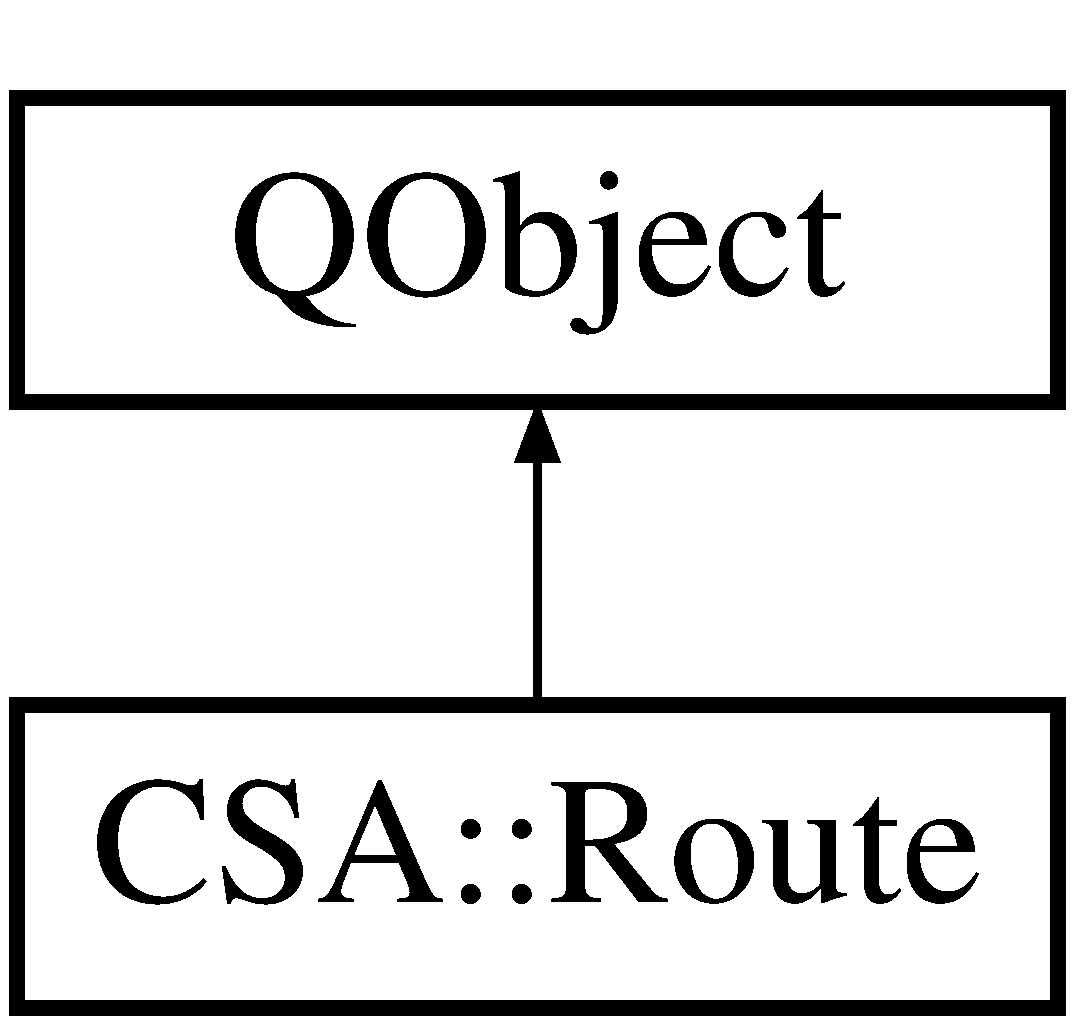
\includegraphics[height=2.000000cm]{classCSA_1_1Route}
\end{center}
\end{figure}
\subsection*{Signals}
\begin{DoxyCompactItemize}
\item 
void \mbox{\hyperlink{classCSA_1_1Route_a6ab64667f4573fd2c9cd8c0b6ab88b46}{legs\+Changed}} ()
\item 
void \mbox{\hyperlink{classCSA_1_1Route_adce4cb4749b3f2668efe082f011a2e47}{transfers\+Changed}} ()
\item 
void \mbox{\hyperlink{classCSA_1_1Route_afe760a3c1e840dfde35219466fa8c5c3}{trip\+Alerts\+Changed}} ()
\item 
void \mbox{\hyperlink{classCSA_1_1Route_a44e976e85e907dfc3b0704c8ce4db5bf}{vehicle\+Alerts\+Changed}} ()
\item 
void \mbox{\hyperlink{classCSA_1_1Route_ab31ce6bceb5dca29f7f74719e50e07df}{remarks\+Changed}} ()
\end{DoxyCompactItemize}
\subsection*{Public Member Functions}
\begin{DoxyCompactItemize}
\item 
\mbox{\hyperlink{classCSA_1_1Route_a285d58821dfce5fe134c928cfb72e56e}{Route}} (const Q\+List$<$ \mbox{\hyperlink{classCSA_1_1RouteLeg}{C\+S\+A\+::\+Route\+Leg}} $\ast$$>$ \&\mbox{\hyperlink{classCSA_1_1Route_aad3e30f3e22b3a1b9d800441ce6ca1d4}{legs}}, const Q\+List$<$ \mbox{\hyperlink{classCSA_1_1Transfer}{C\+S\+A\+::\+Transfer}} $\ast$$>$ \&\mbox{\hyperlink{classCSA_1_1Route_a4a476195f30a740680bd3b61df7a5540}{transfers}}, const Q\+List$<$ \mbox{\hyperlink{classCSA_1_1Message}{C\+S\+A\+::\+Message}} $\ast$$>$ \&\mbox{\hyperlink{classCSA_1_1Route_a6e5c03d04237cea4167239b201f2d40b}{trip\+Alerts}}, const Q\+List$<$ \mbox{\hyperlink{classCSA_1_1Message}{C\+S\+A\+::\+Message}} $\ast$$>$ \&\mbox{\hyperlink{classCSA_1_1Route_a173ce470308b9f20ae2273d987c6041f}{vehicle\+Alerts}}, const Q\+List$<$ \mbox{\hyperlink{classCSA_1_1Message}{C\+S\+A\+::\+Message}} $\ast$$>$ \&\mbox{\hyperlink{classCSA_1_1Route_a6f5f7a812156030f15b7e94b2e43a72a}{remarks}}, Q\+Object $\ast$parent=nullptr)
\item 
\mbox{\hyperlink{classCSA_1_1Route_a9c40376e7b67c123f88b9afba8aad6d6}{Route}} (const Q\+List$<$ \mbox{\hyperlink{classCSA_1_1RouteLeg}{Route\+Leg}} $\ast$$>$ \&\mbox{\hyperlink{classCSA_1_1Route_aad3e30f3e22b3a1b9d800441ce6ca1d4}{legs}}, Q\+Object $\ast$parent=nullptr)
\item 
Q\+List$<$ \mbox{\hyperlink{classCSA_1_1RouteLeg}{C\+S\+A\+::\+Route\+Leg}} $\ast$ $>$ \mbox{\hyperlink{classCSA_1_1Route_aad3e30f3e22b3a1b9d800441ce6ca1d4}{legs}} () const
\item 
void \mbox{\hyperlink{classCSA_1_1Route_acae4554ffa830193e2edbd8936842551}{set\+Legs}} (const Q\+List$<$ \mbox{\hyperlink{classCSA_1_1RouteLeg}{Route\+Leg}} $\ast$$>$ \&\mbox{\hyperlink{classCSA_1_1Route_aad3e30f3e22b3a1b9d800441ce6ca1d4}{legs}})
\item 
Q\+List$<$ \mbox{\hyperlink{classCSA_1_1Transfer}{C\+S\+A\+::\+Transfer}} $\ast$ $>$ \mbox{\hyperlink{classCSA_1_1Route_a4a476195f30a740680bd3b61df7a5540}{transfers}} () const
\item 
void \mbox{\hyperlink{classCSA_1_1Route_a0977183a554295d3aaabdd3e3aa68ab4}{set\+Transfers}} (const Q\+List$<$ \mbox{\hyperlink{classCSA_1_1Transfer}{C\+S\+A\+::\+Transfer}} $\ast$$>$ \&\mbox{\hyperlink{classCSA_1_1Route_a4a476195f30a740680bd3b61df7a5540}{transfers}})
\item 
Q\+List$<$ \mbox{\hyperlink{classCSA_1_1Message}{C\+S\+A\+::\+Message}} $\ast$ $>$ \mbox{\hyperlink{classCSA_1_1Route_a6e5c03d04237cea4167239b201f2d40b}{trip\+Alerts}} () const
\item 
void \mbox{\hyperlink{classCSA_1_1Route_a0ef9be4b744e679ab9daeb8e39753f8f}{set\+Trip\+Alerts}} (const Q\+List$<$ \mbox{\hyperlink{classCSA_1_1Message}{C\+S\+A\+::\+Message}} $\ast$$>$ \&\mbox{\hyperlink{classCSA_1_1Route_a6e5c03d04237cea4167239b201f2d40b}{trip\+Alerts}})
\item 
Q\+List$<$ \mbox{\hyperlink{classCSA_1_1Message}{C\+S\+A\+::\+Message}} $\ast$ $>$ \mbox{\hyperlink{classCSA_1_1Route_a173ce470308b9f20ae2273d987c6041f}{vehicle\+Alerts}} () const
\item 
void \mbox{\hyperlink{classCSA_1_1Route_af9373662a655881774662dd580926e50}{set\+Vehicle\+Alerts}} (const Q\+List$<$ \mbox{\hyperlink{classCSA_1_1Message}{C\+S\+A\+::\+Message}} $\ast$$>$ \&\mbox{\hyperlink{classCSA_1_1Route_a173ce470308b9f20ae2273d987c6041f}{vehicle\+Alerts}})
\item 
Q\+List$<$ \mbox{\hyperlink{classCSA_1_1Message}{C\+S\+A\+::\+Message}} $\ast$ $>$ \mbox{\hyperlink{classCSA_1_1Route_a6f5f7a812156030f15b7e94b2e43a72a}{remarks}} () const
\item 
void \mbox{\hyperlink{classCSA_1_1Route_a285384451bf966a13649e38762205026}{set\+Remarks}} (const Q\+List$<$ \mbox{\hyperlink{classCSA_1_1Message}{C\+S\+A\+::\+Message}} $\ast$$>$ \&\mbox{\hyperlink{classCSA_1_1Route_a6f5f7a812156030f15b7e94b2e43a72a}{remarks}})
\item 
qint64 \mbox{\hyperlink{classCSA_1_1Route_aa23f1a78718f02e17eb409909c6b01b4}{duration}} () const
\item 
qint64 \mbox{\hyperlink{classCSA_1_1Route_a8c89a2514e3f0d0f57ccae96291f33f2}{duration\+With\+Delays}} () const
\item 
Q\+Date\+Time \mbox{\hyperlink{classCSA_1_1Route_ac137b60b8eb1ca666d842d0c7a1e1f1e}{departure\+Time}} () const
\item 
qint16 \mbox{\hyperlink{classCSA_1_1Route_a8773b1afb576a67ba7a76e010aeca537}{departure\+Delay}} () const
\item 
Q\+Date\+Time \mbox{\hyperlink{classCSA_1_1Route_a24964759b1d391a4bb45c7e40daed095}{departure\+Delayed\+Time}} () const
\item 
Q\+Date\+Time \mbox{\hyperlink{classCSA_1_1Route_a29727ecadd5b223b2c34dfe79ae4219a}{arrival\+Time}} () const
\item 
Q\+Date\+Time \mbox{\hyperlink{classCSA_1_1Route_a524f4de8f4eb5dec77acb097ea537d03}{arrival\+Delayed\+Time}} () const
\item 
qint16 \mbox{\hyperlink{classCSA_1_1Route_a02be7800fb68fe82982d71363786550f}{arrival\+Delay}} () const
\item 
qint16 \mbox{\hyperlink{classCSA_1_1Route_ac8e18cd796c135d453e57c1ed0bf4bb9}{transfer\+Count}} () const
\item 
qint16 \mbox{\hyperlink{classCSA_1_1Route_a0f42086c6127684392c8942e4e7bfa66}{station\+Count}} () const
\item 
Q\+String \mbox{\hyperlink{classCSA_1_1Route_af5293d9548b9b9c5879a23e1882a2f33}{departure\+Platform}} () const
\item 
bool \mbox{\hyperlink{classCSA_1_1Route_a0a7f2a3cc8b35d55067ceae8645e3f84}{is\+Departure\+Platform\+Normal}} () const
\item 
Q\+String \mbox{\hyperlink{classCSA_1_1Route_a90d2e37ca55dda6409cd53daaceae002}{arrival\+Platform}} () const
\item 
bool \mbox{\hyperlink{classCSA_1_1Route_a8ce702c2ee2b244be18fd72ec9007410}{is\+Arrival\+Platform\+Normal}} () const
\item 
\mbox{\hyperlink{classCSA_1_1Transfer}{C\+S\+A\+::\+Transfer}} $\ast$ \mbox{\hyperlink{classCSA_1_1Route_a3c17150fb80436b17d1b8874bded6717}{departure\+Station}} () const
\item 
\mbox{\hyperlink{classCSA_1_1Transfer}{C\+S\+A\+::\+Transfer}} $\ast$ \mbox{\hyperlink{classCSA_1_1Route_aef3a9250c98c6283139f261a268e25a9}{arrival\+Station}} () const
\item 
bool \mbox{\hyperlink{classCSA_1_1Route_a5eeb84d448602394e223240ead9a363c}{is\+Partially\+Canceled}} () const
\end{DoxyCompactItemize}
\subsection*{Private Attributes}
\begin{DoxyCompactItemize}
\item 
Q\+List$<$ \mbox{\hyperlink{classCSA_1_1RouteLeg}{C\+S\+A\+::\+Route\+Leg}} $\ast$ $>$ \mbox{\hyperlink{classCSA_1_1Route_a9b5e0351e48fff9dd0d96dc2c06ec186}{m\+\_\+legs}}
\item 
Q\+List$<$ \mbox{\hyperlink{classCSA_1_1Transfer}{C\+S\+A\+::\+Transfer}} $\ast$ $>$ \mbox{\hyperlink{classCSA_1_1Route_a6cda1eec2815597d04332dc00aa02cb5}{m\+\_\+transfers}}
\item 
Q\+List$<$ \mbox{\hyperlink{classCSA_1_1Message}{C\+S\+A\+::\+Message}} $\ast$ $>$ \mbox{\hyperlink{classCSA_1_1Route_a2cc92adcc76332a90cc74816797bed61}{m\+\_\+trip\+Alerts}}
\item 
Q\+List$<$ \mbox{\hyperlink{classCSA_1_1Message}{C\+S\+A\+::\+Message}} $\ast$ $>$ \mbox{\hyperlink{classCSA_1_1Route_a1212f056c45451fa3df603fa1f69e7f4}{m\+\_\+vehicle\+Alerts}}
\item 
Q\+List$<$ \mbox{\hyperlink{classCSA_1_1Message}{C\+S\+A\+::\+Message}} $\ast$ $>$ \mbox{\hyperlink{classCSA_1_1Route_a5826064e86e085944b25d4deb4087ffe}{m\+\_\+remarks}}
\end{DoxyCompactItemize}


\subsection{Constructor \& Destructor Documentation}
\mbox{\Hypertarget{classCSA_1_1Route_a285d58821dfce5fe134c928cfb72e56e}\label{classCSA_1_1Route_a285d58821dfce5fe134c928cfb72e56e}} 
\index{C\+S\+A\+::\+Route@{C\+S\+A\+::\+Route}!Route@{Route}}
\index{Route@{Route}!C\+S\+A\+::\+Route@{C\+S\+A\+::\+Route}}
\subsubsection{\texorpdfstring{Route()}{Route()}\hspace{0.1cm}{\footnotesize\ttfamily [1/2]}}
{\footnotesize\ttfamily C\+S\+A\+::\+Route\+::\+Route (\begin{DoxyParamCaption}\item[{const Q\+List$<$ \mbox{\hyperlink{classCSA_1_1RouteLeg}{C\+S\+A\+::\+Route\+Leg}} $\ast$$>$ \&}]{legs,  }\item[{const Q\+List$<$ \mbox{\hyperlink{classCSA_1_1Transfer}{C\+S\+A\+::\+Transfer}} $\ast$$>$ \&}]{transfers,  }\item[{const Q\+List$<$ \mbox{\hyperlink{classCSA_1_1Message}{C\+S\+A\+::\+Message}} $\ast$$>$ \&}]{trip\+Alerts,  }\item[{const Q\+List$<$ \mbox{\hyperlink{classCSA_1_1Message}{C\+S\+A\+::\+Message}} $\ast$$>$ \&}]{vehicle\+Alerts,  }\item[{const Q\+List$<$ \mbox{\hyperlink{classCSA_1_1Message}{C\+S\+A\+::\+Message}} $\ast$$>$ \&}]{remarks,  }\item[{Q\+Object $\ast$}]{parent = {\ttfamily nullptr} }\end{DoxyParamCaption})\hspace{0.3cm}{\ttfamily [explicit]}}

\mbox{\Hypertarget{classCSA_1_1Route_a9c40376e7b67c123f88b9afba8aad6d6}\label{classCSA_1_1Route_a9c40376e7b67c123f88b9afba8aad6d6}} 
\index{C\+S\+A\+::\+Route@{C\+S\+A\+::\+Route}!Route@{Route}}
\index{Route@{Route}!C\+S\+A\+::\+Route@{C\+S\+A\+::\+Route}}
\subsubsection{\texorpdfstring{Route()}{Route()}\hspace{0.1cm}{\footnotesize\ttfamily [2/2]}}
{\footnotesize\ttfamily C\+S\+A\+::\+Route\+::\+Route (\begin{DoxyParamCaption}\item[{const Q\+List$<$ \mbox{\hyperlink{classCSA_1_1RouteLeg}{Route\+Leg}} $\ast$$>$ \&}]{legs,  }\item[{Q\+Object $\ast$}]{parent = {\ttfamily nullptr} }\end{DoxyParamCaption})\hspace{0.3cm}{\ttfamily [explicit]}}



\subsection{Member Function Documentation}
\mbox{\Hypertarget{classCSA_1_1Route_a02be7800fb68fe82982d71363786550f}\label{classCSA_1_1Route_a02be7800fb68fe82982d71363786550f}} 
\index{C\+S\+A\+::\+Route@{C\+S\+A\+::\+Route}!arrival\+Delay@{arrival\+Delay}}
\index{arrival\+Delay@{arrival\+Delay}!C\+S\+A\+::\+Route@{C\+S\+A\+::\+Route}}
\subsubsection{\texorpdfstring{arrival\+Delay()}{arrivalDelay()}}
{\footnotesize\ttfamily qint16 C\+S\+A\+::\+Route\+::arrival\+Delay (\begin{DoxyParamCaption}{ }\end{DoxyParamCaption}) const}

\mbox{\Hypertarget{classCSA_1_1Route_a524f4de8f4eb5dec77acb097ea537d03}\label{classCSA_1_1Route_a524f4de8f4eb5dec77acb097ea537d03}} 
\index{C\+S\+A\+::\+Route@{C\+S\+A\+::\+Route}!arrival\+Delayed\+Time@{arrival\+Delayed\+Time}}
\index{arrival\+Delayed\+Time@{arrival\+Delayed\+Time}!C\+S\+A\+::\+Route@{C\+S\+A\+::\+Route}}
\subsubsection{\texorpdfstring{arrival\+Delayed\+Time()}{arrivalDelayedTime()}}
{\footnotesize\ttfamily Q\+Date\+Time C\+S\+A\+::\+Route\+::arrival\+Delayed\+Time (\begin{DoxyParamCaption}{ }\end{DoxyParamCaption}) const}

\mbox{\Hypertarget{classCSA_1_1Route_a90d2e37ca55dda6409cd53daaceae002}\label{classCSA_1_1Route_a90d2e37ca55dda6409cd53daaceae002}} 
\index{C\+S\+A\+::\+Route@{C\+S\+A\+::\+Route}!arrival\+Platform@{arrival\+Platform}}
\index{arrival\+Platform@{arrival\+Platform}!C\+S\+A\+::\+Route@{C\+S\+A\+::\+Route}}
\subsubsection{\texorpdfstring{arrival\+Platform()}{arrivalPlatform()}}
{\footnotesize\ttfamily Q\+String C\+S\+A\+::\+Route\+::arrival\+Platform (\begin{DoxyParamCaption}{ }\end{DoxyParamCaption}) const}

\mbox{\Hypertarget{classCSA_1_1Route_aef3a9250c98c6283139f261a268e25a9}\label{classCSA_1_1Route_aef3a9250c98c6283139f261a268e25a9}} 
\index{C\+S\+A\+::\+Route@{C\+S\+A\+::\+Route}!arrival\+Station@{arrival\+Station}}
\index{arrival\+Station@{arrival\+Station}!C\+S\+A\+::\+Route@{C\+S\+A\+::\+Route}}
\subsubsection{\texorpdfstring{arrival\+Station()}{arrivalStation()}}
{\footnotesize\ttfamily \mbox{\hyperlink{classCSA_1_1Transfer}{C\+S\+A\+::\+Transfer}} $\ast$ C\+S\+A\+::\+Route\+::arrival\+Station (\begin{DoxyParamCaption}{ }\end{DoxyParamCaption}) const}

\mbox{\Hypertarget{classCSA_1_1Route_a29727ecadd5b223b2c34dfe79ae4219a}\label{classCSA_1_1Route_a29727ecadd5b223b2c34dfe79ae4219a}} 
\index{C\+S\+A\+::\+Route@{C\+S\+A\+::\+Route}!arrival\+Time@{arrival\+Time}}
\index{arrival\+Time@{arrival\+Time}!C\+S\+A\+::\+Route@{C\+S\+A\+::\+Route}}
\subsubsection{\texorpdfstring{arrival\+Time()}{arrivalTime()}}
{\footnotesize\ttfamily Q\+Date\+Time C\+S\+A\+::\+Route\+::arrival\+Time (\begin{DoxyParamCaption}{ }\end{DoxyParamCaption}) const}

\mbox{\Hypertarget{classCSA_1_1Route_a8773b1afb576a67ba7a76e010aeca537}\label{classCSA_1_1Route_a8773b1afb576a67ba7a76e010aeca537}} 
\index{C\+S\+A\+::\+Route@{C\+S\+A\+::\+Route}!departure\+Delay@{departure\+Delay}}
\index{departure\+Delay@{departure\+Delay}!C\+S\+A\+::\+Route@{C\+S\+A\+::\+Route}}
\subsubsection{\texorpdfstring{departure\+Delay()}{departureDelay()}}
{\footnotesize\ttfamily qint16 C\+S\+A\+::\+Route\+::departure\+Delay (\begin{DoxyParamCaption}{ }\end{DoxyParamCaption}) const}

\mbox{\Hypertarget{classCSA_1_1Route_a24964759b1d391a4bb45c7e40daed095}\label{classCSA_1_1Route_a24964759b1d391a4bb45c7e40daed095}} 
\index{C\+S\+A\+::\+Route@{C\+S\+A\+::\+Route}!departure\+Delayed\+Time@{departure\+Delayed\+Time}}
\index{departure\+Delayed\+Time@{departure\+Delayed\+Time}!C\+S\+A\+::\+Route@{C\+S\+A\+::\+Route}}
\subsubsection{\texorpdfstring{departure\+Delayed\+Time()}{departureDelayedTime()}}
{\footnotesize\ttfamily Q\+Date\+Time C\+S\+A\+::\+Route\+::departure\+Delayed\+Time (\begin{DoxyParamCaption}{ }\end{DoxyParamCaption}) const}

\mbox{\Hypertarget{classCSA_1_1Route_af5293d9548b9b9c5879a23e1882a2f33}\label{classCSA_1_1Route_af5293d9548b9b9c5879a23e1882a2f33}} 
\index{C\+S\+A\+::\+Route@{C\+S\+A\+::\+Route}!departure\+Platform@{departure\+Platform}}
\index{departure\+Platform@{departure\+Platform}!C\+S\+A\+::\+Route@{C\+S\+A\+::\+Route}}
\subsubsection{\texorpdfstring{departure\+Platform()}{departurePlatform()}}
{\footnotesize\ttfamily Q\+String C\+S\+A\+::\+Route\+::departure\+Platform (\begin{DoxyParamCaption}{ }\end{DoxyParamCaption}) const}

\mbox{\Hypertarget{classCSA_1_1Route_a3c17150fb80436b17d1b8874bded6717}\label{classCSA_1_1Route_a3c17150fb80436b17d1b8874bded6717}} 
\index{C\+S\+A\+::\+Route@{C\+S\+A\+::\+Route}!departure\+Station@{departure\+Station}}
\index{departure\+Station@{departure\+Station}!C\+S\+A\+::\+Route@{C\+S\+A\+::\+Route}}
\subsubsection{\texorpdfstring{departure\+Station()}{departureStation()}}
{\footnotesize\ttfamily \mbox{\hyperlink{classCSA_1_1Transfer}{C\+S\+A\+::\+Transfer}} $\ast$ C\+S\+A\+::\+Route\+::departure\+Station (\begin{DoxyParamCaption}{ }\end{DoxyParamCaption}) const}

\mbox{\Hypertarget{classCSA_1_1Route_ac137b60b8eb1ca666d842d0c7a1e1f1e}\label{classCSA_1_1Route_ac137b60b8eb1ca666d842d0c7a1e1f1e}} 
\index{C\+S\+A\+::\+Route@{C\+S\+A\+::\+Route}!departure\+Time@{departure\+Time}}
\index{departure\+Time@{departure\+Time}!C\+S\+A\+::\+Route@{C\+S\+A\+::\+Route}}
\subsubsection{\texorpdfstring{departure\+Time()}{departureTime()}}
{\footnotesize\ttfamily Q\+Date\+Time C\+S\+A\+::\+Route\+::departure\+Time (\begin{DoxyParamCaption}{ }\end{DoxyParamCaption}) const}

\mbox{\Hypertarget{classCSA_1_1Route_aa23f1a78718f02e17eb409909c6b01b4}\label{classCSA_1_1Route_aa23f1a78718f02e17eb409909c6b01b4}} 
\index{C\+S\+A\+::\+Route@{C\+S\+A\+::\+Route}!duration@{duration}}
\index{duration@{duration}!C\+S\+A\+::\+Route@{C\+S\+A\+::\+Route}}
\subsubsection{\texorpdfstring{duration()}{duration()}}
{\footnotesize\ttfamily qint64 C\+S\+A\+::\+Route\+::duration (\begin{DoxyParamCaption}{ }\end{DoxyParamCaption}) const}

\mbox{\Hypertarget{classCSA_1_1Route_a8c89a2514e3f0d0f57ccae96291f33f2}\label{classCSA_1_1Route_a8c89a2514e3f0d0f57ccae96291f33f2}} 
\index{C\+S\+A\+::\+Route@{C\+S\+A\+::\+Route}!duration\+With\+Delays@{duration\+With\+Delays}}
\index{duration\+With\+Delays@{duration\+With\+Delays}!C\+S\+A\+::\+Route@{C\+S\+A\+::\+Route}}
\subsubsection{\texorpdfstring{duration\+With\+Delays()}{durationWithDelays()}}
{\footnotesize\ttfamily qint64 C\+S\+A\+::\+Route\+::duration\+With\+Delays (\begin{DoxyParamCaption}{ }\end{DoxyParamCaption}) const}

\mbox{\Hypertarget{classCSA_1_1Route_a8ce702c2ee2b244be18fd72ec9007410}\label{classCSA_1_1Route_a8ce702c2ee2b244be18fd72ec9007410}} 
\index{C\+S\+A\+::\+Route@{C\+S\+A\+::\+Route}!is\+Arrival\+Platform\+Normal@{is\+Arrival\+Platform\+Normal}}
\index{is\+Arrival\+Platform\+Normal@{is\+Arrival\+Platform\+Normal}!C\+S\+A\+::\+Route@{C\+S\+A\+::\+Route}}
\subsubsection{\texorpdfstring{is\+Arrival\+Platform\+Normal()}{isArrivalPlatformNormal()}}
{\footnotesize\ttfamily bool C\+S\+A\+::\+Route\+::is\+Arrival\+Platform\+Normal (\begin{DoxyParamCaption}{ }\end{DoxyParamCaption}) const}

\mbox{\Hypertarget{classCSA_1_1Route_a0a7f2a3cc8b35d55067ceae8645e3f84}\label{classCSA_1_1Route_a0a7f2a3cc8b35d55067ceae8645e3f84}} 
\index{C\+S\+A\+::\+Route@{C\+S\+A\+::\+Route}!is\+Departure\+Platform\+Normal@{is\+Departure\+Platform\+Normal}}
\index{is\+Departure\+Platform\+Normal@{is\+Departure\+Platform\+Normal}!C\+S\+A\+::\+Route@{C\+S\+A\+::\+Route}}
\subsubsection{\texorpdfstring{is\+Departure\+Platform\+Normal()}{isDeparturePlatformNormal()}}
{\footnotesize\ttfamily bool C\+S\+A\+::\+Route\+::is\+Departure\+Platform\+Normal (\begin{DoxyParamCaption}{ }\end{DoxyParamCaption}) const}

\mbox{\Hypertarget{classCSA_1_1Route_a5eeb84d448602394e223240ead9a363c}\label{classCSA_1_1Route_a5eeb84d448602394e223240ead9a363c}} 
\index{C\+S\+A\+::\+Route@{C\+S\+A\+::\+Route}!is\+Partially\+Canceled@{is\+Partially\+Canceled}}
\index{is\+Partially\+Canceled@{is\+Partially\+Canceled}!C\+S\+A\+::\+Route@{C\+S\+A\+::\+Route}}
\subsubsection{\texorpdfstring{is\+Partially\+Canceled()}{isPartiallyCanceled()}}
{\footnotesize\ttfamily bool C\+S\+A\+::\+Route\+::is\+Partially\+Canceled (\begin{DoxyParamCaption}{ }\end{DoxyParamCaption}) const}

\mbox{\Hypertarget{classCSA_1_1Route_aad3e30f3e22b3a1b9d800441ce6ca1d4}\label{classCSA_1_1Route_aad3e30f3e22b3a1b9d800441ce6ca1d4}} 
\index{C\+S\+A\+::\+Route@{C\+S\+A\+::\+Route}!legs@{legs}}
\index{legs@{legs}!C\+S\+A\+::\+Route@{C\+S\+A\+::\+Route}}
\subsubsection{\texorpdfstring{legs()}{legs()}}
{\footnotesize\ttfamily Q\+List$<$ \mbox{\hyperlink{classCSA_1_1RouteLeg}{C\+S\+A\+::\+Route\+Leg}} $\ast$ $>$ C\+S\+A\+::\+Route\+::legs (\begin{DoxyParamCaption}{ }\end{DoxyParamCaption}) const}

\mbox{\Hypertarget{classCSA_1_1Route_a6ab64667f4573fd2c9cd8c0b6ab88b46}\label{classCSA_1_1Route_a6ab64667f4573fd2c9cd8c0b6ab88b46}} 
\index{C\+S\+A\+::\+Route@{C\+S\+A\+::\+Route}!legs\+Changed@{legs\+Changed}}
\index{legs\+Changed@{legs\+Changed}!C\+S\+A\+::\+Route@{C\+S\+A\+::\+Route}}
\subsubsection{\texorpdfstring{legs\+Changed}{legsChanged}}
{\footnotesize\ttfamily void C\+S\+A\+::\+Route\+::legs\+Changed (\begin{DoxyParamCaption}{ }\end{DoxyParamCaption})\hspace{0.3cm}{\ttfamily [signal]}}

\mbox{\Hypertarget{classCSA_1_1Route_a6f5f7a812156030f15b7e94b2e43a72a}\label{classCSA_1_1Route_a6f5f7a812156030f15b7e94b2e43a72a}} 
\index{C\+S\+A\+::\+Route@{C\+S\+A\+::\+Route}!remarks@{remarks}}
\index{remarks@{remarks}!C\+S\+A\+::\+Route@{C\+S\+A\+::\+Route}}
\subsubsection{\texorpdfstring{remarks()}{remarks()}}
{\footnotesize\ttfamily Q\+List$<$ \mbox{\hyperlink{classCSA_1_1Message}{C\+S\+A\+::\+Message}} $\ast$ $>$ C\+S\+A\+::\+Route\+::remarks (\begin{DoxyParamCaption}{ }\end{DoxyParamCaption}) const}

\mbox{\Hypertarget{classCSA_1_1Route_ab31ce6bceb5dca29f7f74719e50e07df}\label{classCSA_1_1Route_ab31ce6bceb5dca29f7f74719e50e07df}} 
\index{C\+S\+A\+::\+Route@{C\+S\+A\+::\+Route}!remarks\+Changed@{remarks\+Changed}}
\index{remarks\+Changed@{remarks\+Changed}!C\+S\+A\+::\+Route@{C\+S\+A\+::\+Route}}
\subsubsection{\texorpdfstring{remarks\+Changed}{remarksChanged}}
{\footnotesize\ttfamily void C\+S\+A\+::\+Route\+::remarks\+Changed (\begin{DoxyParamCaption}{ }\end{DoxyParamCaption})\hspace{0.3cm}{\ttfamily [signal]}}

\mbox{\Hypertarget{classCSA_1_1Route_acae4554ffa830193e2edbd8936842551}\label{classCSA_1_1Route_acae4554ffa830193e2edbd8936842551}} 
\index{C\+S\+A\+::\+Route@{C\+S\+A\+::\+Route}!set\+Legs@{set\+Legs}}
\index{set\+Legs@{set\+Legs}!C\+S\+A\+::\+Route@{C\+S\+A\+::\+Route}}
\subsubsection{\texorpdfstring{set\+Legs()}{setLegs()}}
{\footnotesize\ttfamily void C\+S\+A\+::\+Route\+::set\+Legs (\begin{DoxyParamCaption}\item[{const Q\+List$<$ \mbox{\hyperlink{classCSA_1_1RouteLeg}{Route\+Leg}} $\ast$$>$ \&}]{legs }\end{DoxyParamCaption})}

\mbox{\Hypertarget{classCSA_1_1Route_a285384451bf966a13649e38762205026}\label{classCSA_1_1Route_a285384451bf966a13649e38762205026}} 
\index{C\+S\+A\+::\+Route@{C\+S\+A\+::\+Route}!set\+Remarks@{set\+Remarks}}
\index{set\+Remarks@{set\+Remarks}!C\+S\+A\+::\+Route@{C\+S\+A\+::\+Route}}
\subsubsection{\texorpdfstring{set\+Remarks()}{setRemarks()}}
{\footnotesize\ttfamily void C\+S\+A\+::\+Route\+::set\+Remarks (\begin{DoxyParamCaption}\item[{const Q\+List$<$ \mbox{\hyperlink{classCSA_1_1Message}{C\+S\+A\+::\+Message}} $\ast$$>$ \&}]{remarks }\end{DoxyParamCaption})}

\mbox{\Hypertarget{classCSA_1_1Route_a0977183a554295d3aaabdd3e3aa68ab4}\label{classCSA_1_1Route_a0977183a554295d3aaabdd3e3aa68ab4}} 
\index{C\+S\+A\+::\+Route@{C\+S\+A\+::\+Route}!set\+Transfers@{set\+Transfers}}
\index{set\+Transfers@{set\+Transfers}!C\+S\+A\+::\+Route@{C\+S\+A\+::\+Route}}
\subsubsection{\texorpdfstring{set\+Transfers()}{setTransfers()}}
{\footnotesize\ttfamily void C\+S\+A\+::\+Route\+::set\+Transfers (\begin{DoxyParamCaption}\item[{const Q\+List$<$ \mbox{\hyperlink{classCSA_1_1Transfer}{C\+S\+A\+::\+Transfer}} $\ast$$>$ \&}]{transfers }\end{DoxyParamCaption})}

\mbox{\Hypertarget{classCSA_1_1Route_a0ef9be4b744e679ab9daeb8e39753f8f}\label{classCSA_1_1Route_a0ef9be4b744e679ab9daeb8e39753f8f}} 
\index{C\+S\+A\+::\+Route@{C\+S\+A\+::\+Route}!set\+Trip\+Alerts@{set\+Trip\+Alerts}}
\index{set\+Trip\+Alerts@{set\+Trip\+Alerts}!C\+S\+A\+::\+Route@{C\+S\+A\+::\+Route}}
\subsubsection{\texorpdfstring{set\+Trip\+Alerts()}{setTripAlerts()}}
{\footnotesize\ttfamily void C\+S\+A\+::\+Route\+::set\+Trip\+Alerts (\begin{DoxyParamCaption}\item[{const Q\+List$<$ \mbox{\hyperlink{classCSA_1_1Message}{C\+S\+A\+::\+Message}} $\ast$$>$ \&}]{trip\+Alerts }\end{DoxyParamCaption})}

\mbox{\Hypertarget{classCSA_1_1Route_af9373662a655881774662dd580926e50}\label{classCSA_1_1Route_af9373662a655881774662dd580926e50}} 
\index{C\+S\+A\+::\+Route@{C\+S\+A\+::\+Route}!set\+Vehicle\+Alerts@{set\+Vehicle\+Alerts}}
\index{set\+Vehicle\+Alerts@{set\+Vehicle\+Alerts}!C\+S\+A\+::\+Route@{C\+S\+A\+::\+Route}}
\subsubsection{\texorpdfstring{set\+Vehicle\+Alerts()}{setVehicleAlerts()}}
{\footnotesize\ttfamily void C\+S\+A\+::\+Route\+::set\+Vehicle\+Alerts (\begin{DoxyParamCaption}\item[{const Q\+List$<$ \mbox{\hyperlink{classCSA_1_1Message}{C\+S\+A\+::\+Message}} $\ast$$>$ \&}]{vehicle\+Alerts }\end{DoxyParamCaption})}

\mbox{\Hypertarget{classCSA_1_1Route_a0f42086c6127684392c8942e4e7bfa66}\label{classCSA_1_1Route_a0f42086c6127684392c8942e4e7bfa66}} 
\index{C\+S\+A\+::\+Route@{C\+S\+A\+::\+Route}!station\+Count@{station\+Count}}
\index{station\+Count@{station\+Count}!C\+S\+A\+::\+Route@{C\+S\+A\+::\+Route}}
\subsubsection{\texorpdfstring{station\+Count()}{stationCount()}}
{\footnotesize\ttfamily qint16 C\+S\+A\+::\+Route\+::station\+Count (\begin{DoxyParamCaption}{ }\end{DoxyParamCaption}) const}

\mbox{\Hypertarget{classCSA_1_1Route_ac8e18cd796c135d453e57c1ed0bf4bb9}\label{classCSA_1_1Route_ac8e18cd796c135d453e57c1ed0bf4bb9}} 
\index{C\+S\+A\+::\+Route@{C\+S\+A\+::\+Route}!transfer\+Count@{transfer\+Count}}
\index{transfer\+Count@{transfer\+Count}!C\+S\+A\+::\+Route@{C\+S\+A\+::\+Route}}
\subsubsection{\texorpdfstring{transfer\+Count()}{transferCount()}}
{\footnotesize\ttfamily qint16 C\+S\+A\+::\+Route\+::transfer\+Count (\begin{DoxyParamCaption}{ }\end{DoxyParamCaption}) const}

\mbox{\Hypertarget{classCSA_1_1Route_a4a476195f30a740680bd3b61df7a5540}\label{classCSA_1_1Route_a4a476195f30a740680bd3b61df7a5540}} 
\index{C\+S\+A\+::\+Route@{C\+S\+A\+::\+Route}!transfers@{transfers}}
\index{transfers@{transfers}!C\+S\+A\+::\+Route@{C\+S\+A\+::\+Route}}
\subsubsection{\texorpdfstring{transfers()}{transfers()}}
{\footnotesize\ttfamily Q\+List$<$ \mbox{\hyperlink{classCSA_1_1Transfer}{C\+S\+A\+::\+Transfer}} $\ast$ $>$ C\+S\+A\+::\+Route\+::transfers (\begin{DoxyParamCaption}{ }\end{DoxyParamCaption}) const}

\mbox{\Hypertarget{classCSA_1_1Route_adce4cb4749b3f2668efe082f011a2e47}\label{classCSA_1_1Route_adce4cb4749b3f2668efe082f011a2e47}} 
\index{C\+S\+A\+::\+Route@{C\+S\+A\+::\+Route}!transfers\+Changed@{transfers\+Changed}}
\index{transfers\+Changed@{transfers\+Changed}!C\+S\+A\+::\+Route@{C\+S\+A\+::\+Route}}
\subsubsection{\texorpdfstring{transfers\+Changed}{transfersChanged}}
{\footnotesize\ttfamily void C\+S\+A\+::\+Route\+::transfers\+Changed (\begin{DoxyParamCaption}{ }\end{DoxyParamCaption})\hspace{0.3cm}{\ttfamily [signal]}}

\mbox{\Hypertarget{classCSA_1_1Route_a6e5c03d04237cea4167239b201f2d40b}\label{classCSA_1_1Route_a6e5c03d04237cea4167239b201f2d40b}} 
\index{C\+S\+A\+::\+Route@{C\+S\+A\+::\+Route}!trip\+Alerts@{trip\+Alerts}}
\index{trip\+Alerts@{trip\+Alerts}!C\+S\+A\+::\+Route@{C\+S\+A\+::\+Route}}
\subsubsection{\texorpdfstring{trip\+Alerts()}{tripAlerts()}}
{\footnotesize\ttfamily Q\+List$<$ \mbox{\hyperlink{classCSA_1_1Message}{C\+S\+A\+::\+Message}} $\ast$ $>$ C\+S\+A\+::\+Route\+::trip\+Alerts (\begin{DoxyParamCaption}{ }\end{DoxyParamCaption}) const}

\mbox{\Hypertarget{classCSA_1_1Route_afe760a3c1e840dfde35219466fa8c5c3}\label{classCSA_1_1Route_afe760a3c1e840dfde35219466fa8c5c3}} 
\index{C\+S\+A\+::\+Route@{C\+S\+A\+::\+Route}!trip\+Alerts\+Changed@{trip\+Alerts\+Changed}}
\index{trip\+Alerts\+Changed@{trip\+Alerts\+Changed}!C\+S\+A\+::\+Route@{C\+S\+A\+::\+Route}}
\subsubsection{\texorpdfstring{trip\+Alerts\+Changed}{tripAlertsChanged}}
{\footnotesize\ttfamily void C\+S\+A\+::\+Route\+::trip\+Alerts\+Changed (\begin{DoxyParamCaption}{ }\end{DoxyParamCaption})\hspace{0.3cm}{\ttfamily [signal]}}

\mbox{\Hypertarget{classCSA_1_1Route_a173ce470308b9f20ae2273d987c6041f}\label{classCSA_1_1Route_a173ce470308b9f20ae2273d987c6041f}} 
\index{C\+S\+A\+::\+Route@{C\+S\+A\+::\+Route}!vehicle\+Alerts@{vehicle\+Alerts}}
\index{vehicle\+Alerts@{vehicle\+Alerts}!C\+S\+A\+::\+Route@{C\+S\+A\+::\+Route}}
\subsubsection{\texorpdfstring{vehicle\+Alerts()}{vehicleAlerts()}}
{\footnotesize\ttfamily Q\+List$<$ \mbox{\hyperlink{classCSA_1_1Message}{C\+S\+A\+::\+Message}} $\ast$ $>$ C\+S\+A\+::\+Route\+::vehicle\+Alerts (\begin{DoxyParamCaption}{ }\end{DoxyParamCaption}) const}

\mbox{\Hypertarget{classCSA_1_1Route_a44e976e85e907dfc3b0704c8ce4db5bf}\label{classCSA_1_1Route_a44e976e85e907dfc3b0704c8ce4db5bf}} 
\index{C\+S\+A\+::\+Route@{C\+S\+A\+::\+Route}!vehicle\+Alerts\+Changed@{vehicle\+Alerts\+Changed}}
\index{vehicle\+Alerts\+Changed@{vehicle\+Alerts\+Changed}!C\+S\+A\+::\+Route@{C\+S\+A\+::\+Route}}
\subsubsection{\texorpdfstring{vehicle\+Alerts\+Changed}{vehicleAlertsChanged}}
{\footnotesize\ttfamily void C\+S\+A\+::\+Route\+::vehicle\+Alerts\+Changed (\begin{DoxyParamCaption}{ }\end{DoxyParamCaption})\hspace{0.3cm}{\ttfamily [signal]}}



\subsection{Member Data Documentation}
\mbox{\Hypertarget{classCSA_1_1Route_a9b5e0351e48fff9dd0d96dc2c06ec186}\label{classCSA_1_1Route_a9b5e0351e48fff9dd0d96dc2c06ec186}} 
\index{C\+S\+A\+::\+Route@{C\+S\+A\+::\+Route}!m\+\_\+legs@{m\+\_\+legs}}
\index{m\+\_\+legs@{m\+\_\+legs}!C\+S\+A\+::\+Route@{C\+S\+A\+::\+Route}}
\subsubsection{\texorpdfstring{m\+\_\+legs}{m\_legs}}
{\footnotesize\ttfamily Q\+List$<$\mbox{\hyperlink{classCSA_1_1RouteLeg}{C\+S\+A\+::\+Route\+Leg}} $\ast$$>$ C\+S\+A\+::\+Route\+::m\+\_\+legs\hspace{0.3cm}{\ttfamily [private]}}

\mbox{\Hypertarget{classCSA_1_1Route_a5826064e86e085944b25d4deb4087ffe}\label{classCSA_1_1Route_a5826064e86e085944b25d4deb4087ffe}} 
\index{C\+S\+A\+::\+Route@{C\+S\+A\+::\+Route}!m\+\_\+remarks@{m\+\_\+remarks}}
\index{m\+\_\+remarks@{m\+\_\+remarks}!C\+S\+A\+::\+Route@{C\+S\+A\+::\+Route}}
\subsubsection{\texorpdfstring{m\+\_\+remarks}{m\_remarks}}
{\footnotesize\ttfamily Q\+List$<$\mbox{\hyperlink{classCSA_1_1Message}{C\+S\+A\+::\+Message}} $\ast$$>$ C\+S\+A\+::\+Route\+::m\+\_\+remarks\hspace{0.3cm}{\ttfamily [private]}}

\mbox{\Hypertarget{classCSA_1_1Route_a6cda1eec2815597d04332dc00aa02cb5}\label{classCSA_1_1Route_a6cda1eec2815597d04332dc00aa02cb5}} 
\index{C\+S\+A\+::\+Route@{C\+S\+A\+::\+Route}!m\+\_\+transfers@{m\+\_\+transfers}}
\index{m\+\_\+transfers@{m\+\_\+transfers}!C\+S\+A\+::\+Route@{C\+S\+A\+::\+Route}}
\subsubsection{\texorpdfstring{m\+\_\+transfers}{m\_transfers}}
{\footnotesize\ttfamily Q\+List$<$\mbox{\hyperlink{classCSA_1_1Transfer}{C\+S\+A\+::\+Transfer}} $\ast$$>$ C\+S\+A\+::\+Route\+::m\+\_\+transfers\hspace{0.3cm}{\ttfamily [private]}}

\mbox{\Hypertarget{classCSA_1_1Route_a2cc92adcc76332a90cc74816797bed61}\label{classCSA_1_1Route_a2cc92adcc76332a90cc74816797bed61}} 
\index{C\+S\+A\+::\+Route@{C\+S\+A\+::\+Route}!m\+\_\+trip\+Alerts@{m\+\_\+trip\+Alerts}}
\index{m\+\_\+trip\+Alerts@{m\+\_\+trip\+Alerts}!C\+S\+A\+::\+Route@{C\+S\+A\+::\+Route}}
\subsubsection{\texorpdfstring{m\+\_\+trip\+Alerts}{m\_tripAlerts}}
{\footnotesize\ttfamily Q\+List$<$\mbox{\hyperlink{classCSA_1_1Message}{C\+S\+A\+::\+Message}} $\ast$$>$ C\+S\+A\+::\+Route\+::m\+\_\+trip\+Alerts\hspace{0.3cm}{\ttfamily [private]}}

\mbox{\Hypertarget{classCSA_1_1Route_a1212f056c45451fa3df603fa1f69e7f4}\label{classCSA_1_1Route_a1212f056c45451fa3df603fa1f69e7f4}} 
\index{C\+S\+A\+::\+Route@{C\+S\+A\+::\+Route}!m\+\_\+vehicle\+Alerts@{m\+\_\+vehicle\+Alerts}}
\index{m\+\_\+vehicle\+Alerts@{m\+\_\+vehicle\+Alerts}!C\+S\+A\+::\+Route@{C\+S\+A\+::\+Route}}
\subsubsection{\texorpdfstring{m\+\_\+vehicle\+Alerts}{m\_vehicleAlerts}}
{\footnotesize\ttfamily Q\+List$<$\mbox{\hyperlink{classCSA_1_1Message}{C\+S\+A\+::\+Message}} $\ast$$>$ C\+S\+A\+::\+Route\+::m\+\_\+vehicle\+Alerts\hspace{0.3cm}{\ttfamily [private]}}



The documentation for this class was generated from the following files\+:\begin{DoxyCompactItemize}
\item 
src/linkedconnections/csa/\mbox{\hyperlink{csaroute_8h}{csaroute.\+h}}\item 
src/linkedconnections/csa/\mbox{\hyperlink{csaroute_8cpp}{csaroute.\+cpp}}\end{DoxyCompactItemize}

\hypertarget{classCSA_1_1RouteLeg}{}\section{C\+SA\+:\+:Route\+Leg Class Reference}
\label{classCSA_1_1RouteLeg}\index{C\+S\+A\+::\+Route\+Leg@{C\+S\+A\+::\+Route\+Leg}}


{\ttfamily \#include $<$csarouteleg.\+h$>$}

Inheritance diagram for C\+SA\+:\+:Route\+Leg\+:\begin{figure}[H]
\begin{center}
\leavevmode
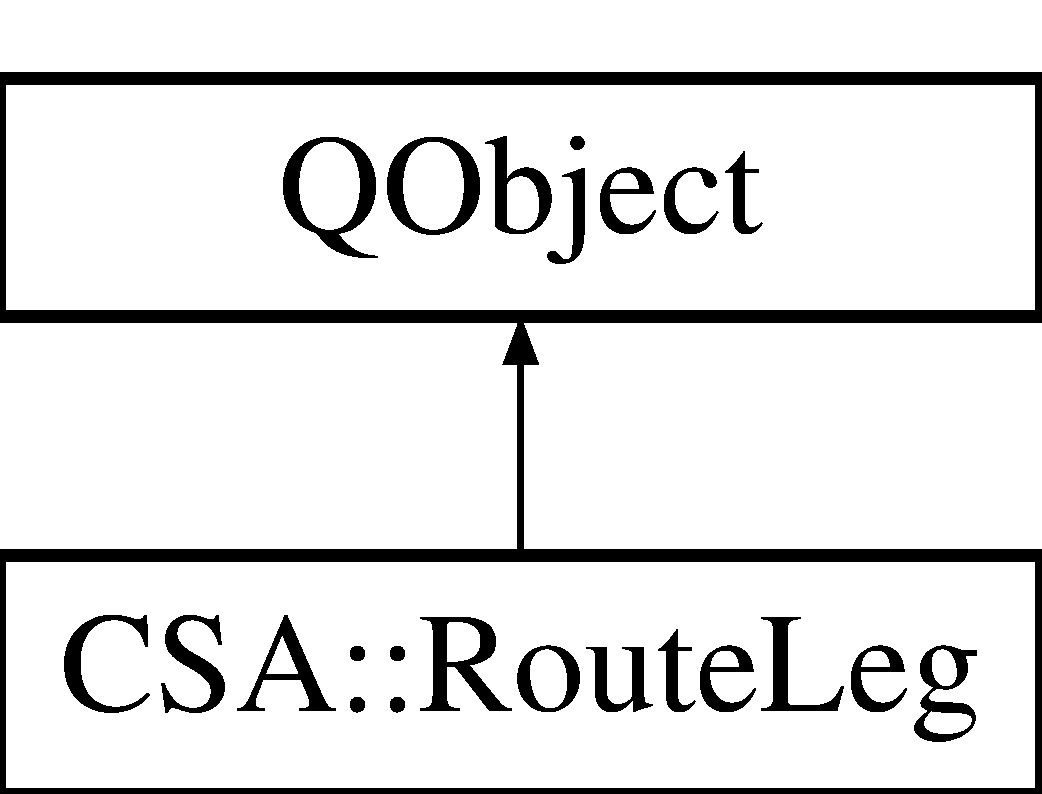
\includegraphics[height=2.000000cm]{classCSA_1_1RouteLeg}
\end{center}
\end{figure}
\subsection*{Public Types}
\begin{DoxyCompactItemize}
\item 
enum \mbox{\hyperlink{classCSA_1_1RouteLeg_a464547cf160a77a2014d101560b1f77b}{Type}} \{ \newline
\mbox{\hyperlink{classCSA_1_1RouteLeg_a464547cf160a77a2014d101560b1f77ba606c114184493a665cf1f6a12fbab9d3}{Type\+::\+W\+A\+L\+K\+I\+NG}}, 
\mbox{\hyperlink{classCSA_1_1RouteLeg_a464547cf160a77a2014d101560b1f77ba4bdeeb2e61c16dbc81956e1bd9148809}{Type\+::\+B\+I\+C\+Y\+C\+LE}}, 
\mbox{\hyperlink{classCSA_1_1RouteLeg_a464547cf160a77a2014d101560b1f77ba0e0c9d888d1093cb2dfa6b25cbce19d8}{Type\+::\+B\+US}}, 
\mbox{\hyperlink{classCSA_1_1RouteLeg_a464547cf160a77a2014d101560b1f77ba0d8fcfacbca6d7ab6fa25ebadb85aa88}{Type\+::\+T\+R\+AM}}, 
\newline
\mbox{\hyperlink{classCSA_1_1RouteLeg_a464547cf160a77a2014d101560b1f77bab7c96478c96d5fff50bc14fb2d33e144}{Type\+::\+M\+E\+T\+RO}}, 
\mbox{\hyperlink{classCSA_1_1RouteLeg_a464547cf160a77a2014d101560b1f77ba45341cc1cc5a485ca18fd816b833175b}{Type\+::\+B\+O\+AT}}, 
\mbox{\hyperlink{classCSA_1_1RouteLeg_a464547cf160a77a2014d101560b1f77ba7086a7774c0003961e43955ec716cb9f}{Type\+::\+T\+A\+XI}}, 
\mbox{\hyperlink{classCSA_1_1RouteLeg_a464547cf160a77a2014d101560b1f77bacf72425b33c7bcc6d1692b0793e1a8b1}{Type\+::\+T\+R\+A\+IN}}
 \}
\end{DoxyCompactItemize}
\subsection*{Signals}
\begin{DoxyCompactItemize}
\item 
void \mbox{\hyperlink{classCSA_1_1RouteLeg_a5ea5eef9f78700d451ddd2f0ad0ac208}{type\+Changed}} ()
\item 
void \mbox{\hyperlink{classCSA_1_1RouteLeg_abf2e225d549710146cdee9548d1c76c3}{vehicle\+Information\+Changed}} ()
\item 
void \mbox{\hyperlink{classCSA_1_1RouteLeg_a1369506613524120c93e6b5932a7ad95}{intermediary\+Stops\+Changed}} ()
\item 
void \mbox{\hyperlink{classCSA_1_1RouteLeg_a092966483399a1c895945178ed1353cf}{stops\+Changed}} ()
\item 
void \mbox{\hyperlink{classCSA_1_1RouteLeg_a7f70b16edb2c9aff18d75e7ea06e5d01}{departure\+Changed}} ()
\item 
void \mbox{\hyperlink{classCSA_1_1RouteLeg_a1163b0c9b0b0020677776c576b2fd73b}{arrival\+Changed}} ()
\item 
void \mbox{\hyperlink{classCSA_1_1RouteLeg_a0e0cfc76d7282cdedc17bf170b8a477d}{station\+Changed}} ()
\end{DoxyCompactItemize}
\subsection*{Public Member Functions}
\begin{DoxyCompactItemize}
\item 
\mbox{\hyperlink{classCSA_1_1RouteLeg_a81e25540ddee7870c6304c6e6efd8490}{Route\+Leg}} (const \mbox{\hyperlink{classCSA_1_1RouteLeg_a464547cf160a77a2014d101560b1f77b}{C\+S\+A\+::\+Route\+Leg\+::\+Type}} \&\mbox{\hyperlink{classCSA_1_1RouteLeg_abbea7d9d097dbf9b7c87543b2a2e8aac}{type}}, \mbox{\hyperlink{classCSA_1_1Vehicle}{C\+S\+A\+::\+Vehicle}} $\ast$\mbox{\hyperlink{classCSA_1_1RouteLeg_a766608f69057a64427736f02de434654}{vehicle\+Information}}, \mbox{\hyperlink{classCSA_1_1RouteLegEnd}{C\+S\+A\+::\+Route\+Leg\+End}} $\ast$\mbox{\hyperlink{classCSA_1_1RouteLeg_adc49bfe6b5aef6f5a2c2bffa72540308}{departure}}, \mbox{\hyperlink{classCSA_1_1RouteLegEnd}{C\+S\+A\+::\+Route\+Leg\+End}} $\ast$\mbox{\hyperlink{classCSA_1_1RouteLeg_a096f128bcfa0e616bfab643f5b2c245f}{arrival}}, Q\+Object $\ast$parent=nullptr)
\item 
\mbox{\hyperlink{classCSA_1_1RouteLeg_a464547cf160a77a2014d101560b1f77b}{C\+S\+A\+::\+Route\+Leg\+::\+Type}} \mbox{\hyperlink{classCSA_1_1RouteLeg_abbea7d9d097dbf9b7c87543b2a2e8aac}{type}} () const
\item 
void \mbox{\hyperlink{classCSA_1_1RouteLeg_a8a175ba408df0aeb3a345f57ce65db5b}{set\+Type}} (const \mbox{\hyperlink{classCSA_1_1RouteLeg_a464547cf160a77a2014d101560b1f77b}{C\+S\+A\+::\+Route\+Leg\+::\+Type}} \&\mbox{\hyperlink{classCSA_1_1RouteLeg_abbea7d9d097dbf9b7c87543b2a2e8aac}{type}})
\item 
\mbox{\hyperlink{classCSA_1_1Vehicle}{C\+S\+A\+::\+Vehicle}} $\ast$ \mbox{\hyperlink{classCSA_1_1RouteLeg_a766608f69057a64427736f02de434654}{vehicle\+Information}} () const
\item 
void \mbox{\hyperlink{classCSA_1_1RouteLeg_a88faef67ebfa683c1ea15f8e672f16c3}{set\+Vehicle\+Information}} (\mbox{\hyperlink{classCSA_1_1Vehicle}{C\+S\+A\+::\+Vehicle}} $\ast$\mbox{\hyperlink{classCSA_1_1RouteLeg_a766608f69057a64427736f02de434654}{vehicle\+Information}})
\item 
Q\+List$<$ \mbox{\hyperlink{classCSA_1_1VehicleStop}{C\+S\+A\+::\+Vehicle\+Stop}} $\ast$ $>$ \mbox{\hyperlink{classCSA_1_1RouteLeg_a6cb78630def68232e02545f8803c7a27}{intermediary\+Stops}} () const
\item 
void \mbox{\hyperlink{classCSA_1_1RouteLeg_aa01b151e07580a55b7fec9a1cadfc9bb}{set\+Intermediary\+Stops}} (const Q\+List$<$ \mbox{\hyperlink{classCSA_1_1VehicleStop}{C\+S\+A\+::\+Vehicle\+Stop}} $\ast$$>$ \&\mbox{\hyperlink{classCSA_1_1RouteLeg_a6cb78630def68232e02545f8803c7a27}{intermediary\+Stops}})
\item 
\mbox{\hyperlink{classCSA_1_1RouteLegEnd}{C\+S\+A\+::\+Route\+Leg\+End}} $\ast$ \mbox{\hyperlink{classCSA_1_1RouteLeg_adc49bfe6b5aef6f5a2c2bffa72540308}{departure}} () const
\item 
void \mbox{\hyperlink{classCSA_1_1RouteLeg_a3cebb4e61aea81676361abbff9b723d1}{set\+Departure}} (\mbox{\hyperlink{classCSA_1_1RouteLegEnd}{C\+S\+A\+::\+Route\+Leg\+End}} $\ast$\mbox{\hyperlink{classCSA_1_1RouteLeg_adc49bfe6b5aef6f5a2c2bffa72540308}{departure}})
\item 
\mbox{\hyperlink{classCSA_1_1RouteLegEnd}{C\+S\+A\+::\+Route\+Leg\+End}} $\ast$ \mbox{\hyperlink{classCSA_1_1RouteLeg_a096f128bcfa0e616bfab643f5b2c245f}{arrival}} () const
\item 
void \mbox{\hyperlink{classCSA_1_1RouteLeg_a6c3a8bc9a6e8c89c797613d59758404c}{set\+Arrival}} (\mbox{\hyperlink{classCSA_1_1RouteLegEnd}{C\+S\+A\+::\+Route\+Leg\+End}} $\ast$\mbox{\hyperlink{classCSA_1_1RouteLeg_a096f128bcfa0e616bfab643f5b2c245f}{arrival}})
\item 
\mbox{\hyperlink{classCSA_1_1Station}{C\+S\+A\+::\+Station}} $\ast$ \mbox{\hyperlink{classCSA_1_1RouteLeg_a6e018b382168cc05db7088873093cfde}{station}} () const
\end{DoxyCompactItemize}
\subsection*{Private Attributes}
\begin{DoxyCompactItemize}
\item 
\mbox{\hyperlink{classCSA_1_1RouteLeg_a464547cf160a77a2014d101560b1f77b}{C\+S\+A\+::\+Route\+Leg\+::\+Type}} \mbox{\hyperlink{classCSA_1_1RouteLeg_afa6addf2a813318e92228221f8588e36}{m\+\_\+type}}
\item 
\mbox{\hyperlink{classCSA_1_1Vehicle}{C\+S\+A\+::\+Vehicle}} $\ast$ \mbox{\hyperlink{classCSA_1_1RouteLeg_a6386eed3d1176ed734ca3fdc589cb90f}{m\+\_\+vehicle\+Information}}
\item 
Q\+List$<$ \mbox{\hyperlink{classCSA_1_1VehicleStop}{C\+S\+A\+::\+Vehicle\+Stop}} $\ast$ $>$ \mbox{\hyperlink{classCSA_1_1RouteLeg_adb7b64dcb19e7358d822ff807d1e8a52}{m\+\_\+intermediary\+Stops}}
\item 
\mbox{\hyperlink{classCSA_1_1RouteLegEnd}{C\+S\+A\+::\+Route\+Leg\+End}} $\ast$ \mbox{\hyperlink{classCSA_1_1RouteLeg_ab230f54abd48e7bb23888e0b32543a6b}{m\+\_\+departure}}
\item 
\mbox{\hyperlink{classCSA_1_1RouteLegEnd}{C\+S\+A\+::\+Route\+Leg\+End}} $\ast$ \mbox{\hyperlink{classCSA_1_1RouteLeg_a19d5e45a31fddee3bdb949af4b6fa2a6}{m\+\_\+arrival}}
\end{DoxyCompactItemize}


\subsection{Member Enumeration Documentation}
\mbox{\Hypertarget{classCSA_1_1RouteLeg_a464547cf160a77a2014d101560b1f77b}\label{classCSA_1_1RouteLeg_a464547cf160a77a2014d101560b1f77b}} 
\index{C\+S\+A\+::\+Route\+Leg@{C\+S\+A\+::\+Route\+Leg}!Type@{Type}}
\index{Type@{Type}!C\+S\+A\+::\+Route\+Leg@{C\+S\+A\+::\+Route\+Leg}}
\subsubsection{\texorpdfstring{Type}{Type}}
{\footnotesize\ttfamily enum \mbox{\hyperlink{classCSA_1_1RouteLeg_a464547cf160a77a2014d101560b1f77b}{C\+S\+A\+::\+Route\+Leg\+::\+Type}}\hspace{0.3cm}{\ttfamily [strong]}}

\begin{DoxyEnumFields}{Enumerator}
\raisebox{\heightof{T}}[0pt][0pt]{\index{W\+A\+L\+K\+I\+NG@{W\+A\+L\+K\+I\+NG}!C\+S\+A\+::\+Route\+Leg@{C\+S\+A\+::\+Route\+Leg}}\index{C\+S\+A\+::\+Route\+Leg@{C\+S\+A\+::\+Route\+Leg}!W\+A\+L\+K\+I\+NG@{W\+A\+L\+K\+I\+NG}}}\mbox{\Hypertarget{classCSA_1_1RouteLeg_a464547cf160a77a2014d101560b1f77ba606c114184493a665cf1f6a12fbab9d3}\label{classCSA_1_1RouteLeg_a464547cf160a77a2014d101560b1f77ba606c114184493a665cf1f6a12fbab9d3}} 
W\+A\+L\+K\+I\+NG&\\
\hline

\raisebox{\heightof{T}}[0pt][0pt]{\index{B\+I\+C\+Y\+C\+LE@{B\+I\+C\+Y\+C\+LE}!C\+S\+A\+::\+Route\+Leg@{C\+S\+A\+::\+Route\+Leg}}\index{C\+S\+A\+::\+Route\+Leg@{C\+S\+A\+::\+Route\+Leg}!B\+I\+C\+Y\+C\+LE@{B\+I\+C\+Y\+C\+LE}}}\mbox{\Hypertarget{classCSA_1_1RouteLeg_a464547cf160a77a2014d101560b1f77ba4bdeeb2e61c16dbc81956e1bd9148809}\label{classCSA_1_1RouteLeg_a464547cf160a77a2014d101560b1f77ba4bdeeb2e61c16dbc81956e1bd9148809}} 
B\+I\+C\+Y\+C\+LE&\\
\hline

\raisebox{\heightof{T}}[0pt][0pt]{\index{B\+US@{B\+US}!C\+S\+A\+::\+Route\+Leg@{C\+S\+A\+::\+Route\+Leg}}\index{C\+S\+A\+::\+Route\+Leg@{C\+S\+A\+::\+Route\+Leg}!B\+US@{B\+US}}}\mbox{\Hypertarget{classCSA_1_1RouteLeg_a464547cf160a77a2014d101560b1f77ba0e0c9d888d1093cb2dfa6b25cbce19d8}\label{classCSA_1_1RouteLeg_a464547cf160a77a2014d101560b1f77ba0e0c9d888d1093cb2dfa6b25cbce19d8}} 
B\+US&\\
\hline

\raisebox{\heightof{T}}[0pt][0pt]{\index{T\+R\+AM@{T\+R\+AM}!C\+S\+A\+::\+Route\+Leg@{C\+S\+A\+::\+Route\+Leg}}\index{C\+S\+A\+::\+Route\+Leg@{C\+S\+A\+::\+Route\+Leg}!T\+R\+AM@{T\+R\+AM}}}\mbox{\Hypertarget{classCSA_1_1RouteLeg_a464547cf160a77a2014d101560b1f77ba0d8fcfacbca6d7ab6fa25ebadb85aa88}\label{classCSA_1_1RouteLeg_a464547cf160a77a2014d101560b1f77ba0d8fcfacbca6d7ab6fa25ebadb85aa88}} 
T\+R\+AM&\\
\hline

\raisebox{\heightof{T}}[0pt][0pt]{\index{M\+E\+T\+RO@{M\+E\+T\+RO}!C\+S\+A\+::\+Route\+Leg@{C\+S\+A\+::\+Route\+Leg}}\index{C\+S\+A\+::\+Route\+Leg@{C\+S\+A\+::\+Route\+Leg}!M\+E\+T\+RO@{M\+E\+T\+RO}}}\mbox{\Hypertarget{classCSA_1_1RouteLeg_a464547cf160a77a2014d101560b1f77bab7c96478c96d5fff50bc14fb2d33e144}\label{classCSA_1_1RouteLeg_a464547cf160a77a2014d101560b1f77bab7c96478c96d5fff50bc14fb2d33e144}} 
M\+E\+T\+RO&\\
\hline

\raisebox{\heightof{T}}[0pt][0pt]{\index{B\+O\+AT@{B\+O\+AT}!C\+S\+A\+::\+Route\+Leg@{C\+S\+A\+::\+Route\+Leg}}\index{C\+S\+A\+::\+Route\+Leg@{C\+S\+A\+::\+Route\+Leg}!B\+O\+AT@{B\+O\+AT}}}\mbox{\Hypertarget{classCSA_1_1RouteLeg_a464547cf160a77a2014d101560b1f77ba45341cc1cc5a485ca18fd816b833175b}\label{classCSA_1_1RouteLeg_a464547cf160a77a2014d101560b1f77ba45341cc1cc5a485ca18fd816b833175b}} 
B\+O\+AT&\\
\hline

\raisebox{\heightof{T}}[0pt][0pt]{\index{T\+A\+XI@{T\+A\+XI}!C\+S\+A\+::\+Route\+Leg@{C\+S\+A\+::\+Route\+Leg}}\index{C\+S\+A\+::\+Route\+Leg@{C\+S\+A\+::\+Route\+Leg}!T\+A\+XI@{T\+A\+XI}}}\mbox{\Hypertarget{classCSA_1_1RouteLeg_a464547cf160a77a2014d101560b1f77ba7086a7774c0003961e43955ec716cb9f}\label{classCSA_1_1RouteLeg_a464547cf160a77a2014d101560b1f77ba7086a7774c0003961e43955ec716cb9f}} 
T\+A\+XI&\\
\hline

\raisebox{\heightof{T}}[0pt][0pt]{\index{T\+R\+A\+IN@{T\+R\+A\+IN}!C\+S\+A\+::\+Route\+Leg@{C\+S\+A\+::\+Route\+Leg}}\index{C\+S\+A\+::\+Route\+Leg@{C\+S\+A\+::\+Route\+Leg}!T\+R\+A\+IN@{T\+R\+A\+IN}}}\mbox{\Hypertarget{classCSA_1_1RouteLeg_a464547cf160a77a2014d101560b1f77bacf72425b33c7bcc6d1692b0793e1a8b1}\label{classCSA_1_1RouteLeg_a464547cf160a77a2014d101560b1f77bacf72425b33c7bcc6d1692b0793e1a8b1}} 
T\+R\+A\+IN&\\
\hline

\end{DoxyEnumFields}


\subsection{Constructor \& Destructor Documentation}
\mbox{\Hypertarget{classCSA_1_1RouteLeg_a81e25540ddee7870c6304c6e6efd8490}\label{classCSA_1_1RouteLeg_a81e25540ddee7870c6304c6e6efd8490}} 
\index{C\+S\+A\+::\+Route\+Leg@{C\+S\+A\+::\+Route\+Leg}!Route\+Leg@{Route\+Leg}}
\index{Route\+Leg@{Route\+Leg}!C\+S\+A\+::\+Route\+Leg@{C\+S\+A\+::\+Route\+Leg}}
\subsubsection{\texorpdfstring{Route\+Leg()}{RouteLeg()}}
{\footnotesize\ttfamily C\+S\+A\+::\+Route\+Leg\+::\+Route\+Leg (\begin{DoxyParamCaption}\item[{const \mbox{\hyperlink{classCSA_1_1RouteLeg_a464547cf160a77a2014d101560b1f77b}{C\+S\+A\+::\+Route\+Leg\+::\+Type}} \&}]{type,  }\item[{\mbox{\hyperlink{classCSA_1_1Vehicle}{C\+S\+A\+::\+Vehicle}} $\ast$}]{vehicle\+Information,  }\item[{\mbox{\hyperlink{classCSA_1_1RouteLegEnd}{C\+S\+A\+::\+Route\+Leg\+End}} $\ast$}]{departure,  }\item[{\mbox{\hyperlink{classCSA_1_1RouteLegEnd}{C\+S\+A\+::\+Route\+Leg\+End}} $\ast$}]{arrival,  }\item[{Q\+Object $\ast$}]{parent = {\ttfamily nullptr} }\end{DoxyParamCaption})\hspace{0.3cm}{\ttfamily [explicit]}}



\subsection{Member Function Documentation}
\mbox{\Hypertarget{classCSA_1_1RouteLeg_a096f128bcfa0e616bfab643f5b2c245f}\label{classCSA_1_1RouteLeg_a096f128bcfa0e616bfab643f5b2c245f}} 
\index{C\+S\+A\+::\+Route\+Leg@{C\+S\+A\+::\+Route\+Leg}!arrival@{arrival}}
\index{arrival@{arrival}!C\+S\+A\+::\+Route\+Leg@{C\+S\+A\+::\+Route\+Leg}}
\subsubsection{\texorpdfstring{arrival()}{arrival()}}
{\footnotesize\ttfamily \mbox{\hyperlink{classCSA_1_1RouteLegEnd}{C\+S\+A\+::\+Route\+Leg\+End}} $\ast$ C\+S\+A\+::\+Route\+Leg\+::arrival (\begin{DoxyParamCaption}{ }\end{DoxyParamCaption}) const}

\mbox{\Hypertarget{classCSA_1_1RouteLeg_a1163b0c9b0b0020677776c576b2fd73b}\label{classCSA_1_1RouteLeg_a1163b0c9b0b0020677776c576b2fd73b}} 
\index{C\+S\+A\+::\+Route\+Leg@{C\+S\+A\+::\+Route\+Leg}!arrival\+Changed@{arrival\+Changed}}
\index{arrival\+Changed@{arrival\+Changed}!C\+S\+A\+::\+Route\+Leg@{C\+S\+A\+::\+Route\+Leg}}
\subsubsection{\texorpdfstring{arrival\+Changed}{arrivalChanged}}
{\footnotesize\ttfamily void C\+S\+A\+::\+Route\+Leg\+::arrival\+Changed (\begin{DoxyParamCaption}{ }\end{DoxyParamCaption})\hspace{0.3cm}{\ttfamily [signal]}}

\mbox{\Hypertarget{classCSA_1_1RouteLeg_adc49bfe6b5aef6f5a2c2bffa72540308}\label{classCSA_1_1RouteLeg_adc49bfe6b5aef6f5a2c2bffa72540308}} 
\index{C\+S\+A\+::\+Route\+Leg@{C\+S\+A\+::\+Route\+Leg}!departure@{departure}}
\index{departure@{departure}!C\+S\+A\+::\+Route\+Leg@{C\+S\+A\+::\+Route\+Leg}}
\subsubsection{\texorpdfstring{departure()}{departure()}}
{\footnotesize\ttfamily \mbox{\hyperlink{classCSA_1_1RouteLegEnd}{C\+S\+A\+::\+Route\+Leg\+End}} $\ast$ C\+S\+A\+::\+Route\+Leg\+::departure (\begin{DoxyParamCaption}{ }\end{DoxyParamCaption}) const}

\mbox{\Hypertarget{classCSA_1_1RouteLeg_a7f70b16edb2c9aff18d75e7ea06e5d01}\label{classCSA_1_1RouteLeg_a7f70b16edb2c9aff18d75e7ea06e5d01}} 
\index{C\+S\+A\+::\+Route\+Leg@{C\+S\+A\+::\+Route\+Leg}!departure\+Changed@{departure\+Changed}}
\index{departure\+Changed@{departure\+Changed}!C\+S\+A\+::\+Route\+Leg@{C\+S\+A\+::\+Route\+Leg}}
\subsubsection{\texorpdfstring{departure\+Changed}{departureChanged}}
{\footnotesize\ttfamily void C\+S\+A\+::\+Route\+Leg\+::departure\+Changed (\begin{DoxyParamCaption}{ }\end{DoxyParamCaption})\hspace{0.3cm}{\ttfamily [signal]}}

\mbox{\Hypertarget{classCSA_1_1RouteLeg_a6cb78630def68232e02545f8803c7a27}\label{classCSA_1_1RouteLeg_a6cb78630def68232e02545f8803c7a27}} 
\index{C\+S\+A\+::\+Route\+Leg@{C\+S\+A\+::\+Route\+Leg}!intermediary\+Stops@{intermediary\+Stops}}
\index{intermediary\+Stops@{intermediary\+Stops}!C\+S\+A\+::\+Route\+Leg@{C\+S\+A\+::\+Route\+Leg}}
\subsubsection{\texorpdfstring{intermediary\+Stops()}{intermediaryStops()}}
{\footnotesize\ttfamily Q\+List$<$ \mbox{\hyperlink{classCSA_1_1VehicleStop}{C\+S\+A\+::\+Vehicle\+Stop}} $\ast$ $>$ C\+S\+A\+::\+Route\+Leg\+::intermediary\+Stops (\begin{DoxyParamCaption}{ }\end{DoxyParamCaption}) const}

\mbox{\Hypertarget{classCSA_1_1RouteLeg_a1369506613524120c93e6b5932a7ad95}\label{classCSA_1_1RouteLeg_a1369506613524120c93e6b5932a7ad95}} 
\index{C\+S\+A\+::\+Route\+Leg@{C\+S\+A\+::\+Route\+Leg}!intermediary\+Stops\+Changed@{intermediary\+Stops\+Changed}}
\index{intermediary\+Stops\+Changed@{intermediary\+Stops\+Changed}!C\+S\+A\+::\+Route\+Leg@{C\+S\+A\+::\+Route\+Leg}}
\subsubsection{\texorpdfstring{intermediary\+Stops\+Changed}{intermediaryStopsChanged}}
{\footnotesize\ttfamily void C\+S\+A\+::\+Route\+Leg\+::intermediary\+Stops\+Changed (\begin{DoxyParamCaption}{ }\end{DoxyParamCaption})\hspace{0.3cm}{\ttfamily [signal]}}

\mbox{\Hypertarget{classCSA_1_1RouteLeg_a6c3a8bc9a6e8c89c797613d59758404c}\label{classCSA_1_1RouteLeg_a6c3a8bc9a6e8c89c797613d59758404c}} 
\index{C\+S\+A\+::\+Route\+Leg@{C\+S\+A\+::\+Route\+Leg}!set\+Arrival@{set\+Arrival}}
\index{set\+Arrival@{set\+Arrival}!C\+S\+A\+::\+Route\+Leg@{C\+S\+A\+::\+Route\+Leg}}
\subsubsection{\texorpdfstring{set\+Arrival()}{setArrival()}}
{\footnotesize\ttfamily void C\+S\+A\+::\+Route\+Leg\+::set\+Arrival (\begin{DoxyParamCaption}\item[{\mbox{\hyperlink{classCSA_1_1RouteLegEnd}{C\+S\+A\+::\+Route\+Leg\+End}} $\ast$}]{arrival }\end{DoxyParamCaption})}

\mbox{\Hypertarget{classCSA_1_1RouteLeg_a3cebb4e61aea81676361abbff9b723d1}\label{classCSA_1_1RouteLeg_a3cebb4e61aea81676361abbff9b723d1}} 
\index{C\+S\+A\+::\+Route\+Leg@{C\+S\+A\+::\+Route\+Leg}!set\+Departure@{set\+Departure}}
\index{set\+Departure@{set\+Departure}!C\+S\+A\+::\+Route\+Leg@{C\+S\+A\+::\+Route\+Leg}}
\subsubsection{\texorpdfstring{set\+Departure()}{setDeparture()}}
{\footnotesize\ttfamily void C\+S\+A\+::\+Route\+Leg\+::set\+Departure (\begin{DoxyParamCaption}\item[{\mbox{\hyperlink{classCSA_1_1RouteLegEnd}{C\+S\+A\+::\+Route\+Leg\+End}} $\ast$}]{departure }\end{DoxyParamCaption})}

\mbox{\Hypertarget{classCSA_1_1RouteLeg_aa01b151e07580a55b7fec9a1cadfc9bb}\label{classCSA_1_1RouteLeg_aa01b151e07580a55b7fec9a1cadfc9bb}} 
\index{C\+S\+A\+::\+Route\+Leg@{C\+S\+A\+::\+Route\+Leg}!set\+Intermediary\+Stops@{set\+Intermediary\+Stops}}
\index{set\+Intermediary\+Stops@{set\+Intermediary\+Stops}!C\+S\+A\+::\+Route\+Leg@{C\+S\+A\+::\+Route\+Leg}}
\subsubsection{\texorpdfstring{set\+Intermediary\+Stops()}{setIntermediaryStops()}}
{\footnotesize\ttfamily void C\+S\+A\+::\+Route\+Leg\+::set\+Intermediary\+Stops (\begin{DoxyParamCaption}\item[{const Q\+List$<$ \mbox{\hyperlink{classCSA_1_1VehicleStop}{C\+S\+A\+::\+Vehicle\+Stop}} $\ast$$>$ \&}]{intermediary\+Stops }\end{DoxyParamCaption})}

\mbox{\Hypertarget{classCSA_1_1RouteLeg_a8a175ba408df0aeb3a345f57ce65db5b}\label{classCSA_1_1RouteLeg_a8a175ba408df0aeb3a345f57ce65db5b}} 
\index{C\+S\+A\+::\+Route\+Leg@{C\+S\+A\+::\+Route\+Leg}!set\+Type@{set\+Type}}
\index{set\+Type@{set\+Type}!C\+S\+A\+::\+Route\+Leg@{C\+S\+A\+::\+Route\+Leg}}
\subsubsection{\texorpdfstring{set\+Type()}{setType()}}
{\footnotesize\ttfamily void C\+S\+A\+::\+Route\+Leg\+::set\+Type (\begin{DoxyParamCaption}\item[{const \mbox{\hyperlink{classCSA_1_1RouteLeg_a464547cf160a77a2014d101560b1f77b}{C\+S\+A\+::\+Route\+Leg\+::\+Type}} \&}]{type }\end{DoxyParamCaption})}

\mbox{\Hypertarget{classCSA_1_1RouteLeg_a88faef67ebfa683c1ea15f8e672f16c3}\label{classCSA_1_1RouteLeg_a88faef67ebfa683c1ea15f8e672f16c3}} 
\index{C\+S\+A\+::\+Route\+Leg@{C\+S\+A\+::\+Route\+Leg}!set\+Vehicle\+Information@{set\+Vehicle\+Information}}
\index{set\+Vehicle\+Information@{set\+Vehicle\+Information}!C\+S\+A\+::\+Route\+Leg@{C\+S\+A\+::\+Route\+Leg}}
\subsubsection{\texorpdfstring{set\+Vehicle\+Information()}{setVehicleInformation()}}
{\footnotesize\ttfamily void C\+S\+A\+::\+Route\+Leg\+::set\+Vehicle\+Information (\begin{DoxyParamCaption}\item[{\mbox{\hyperlink{classCSA_1_1Vehicle}{C\+S\+A\+::\+Vehicle}} $\ast$}]{vehicle\+Information }\end{DoxyParamCaption})}

\mbox{\Hypertarget{classCSA_1_1RouteLeg_a6e018b382168cc05db7088873093cfde}\label{classCSA_1_1RouteLeg_a6e018b382168cc05db7088873093cfde}} 
\index{C\+S\+A\+::\+Route\+Leg@{C\+S\+A\+::\+Route\+Leg}!station@{station}}
\index{station@{station}!C\+S\+A\+::\+Route\+Leg@{C\+S\+A\+::\+Route\+Leg}}
\subsubsection{\texorpdfstring{station()}{station()}}
{\footnotesize\ttfamily \mbox{\hyperlink{classCSA_1_1Station}{C\+S\+A\+::\+Station}} $\ast$ C\+S\+A\+::\+Route\+Leg\+::station (\begin{DoxyParamCaption}{ }\end{DoxyParamCaption}) const}

\mbox{\Hypertarget{classCSA_1_1RouteLeg_a0e0cfc76d7282cdedc17bf170b8a477d}\label{classCSA_1_1RouteLeg_a0e0cfc76d7282cdedc17bf170b8a477d}} 
\index{C\+S\+A\+::\+Route\+Leg@{C\+S\+A\+::\+Route\+Leg}!station\+Changed@{station\+Changed}}
\index{station\+Changed@{station\+Changed}!C\+S\+A\+::\+Route\+Leg@{C\+S\+A\+::\+Route\+Leg}}
\subsubsection{\texorpdfstring{station\+Changed}{stationChanged}}
{\footnotesize\ttfamily void C\+S\+A\+::\+Route\+Leg\+::station\+Changed (\begin{DoxyParamCaption}{ }\end{DoxyParamCaption})\hspace{0.3cm}{\ttfamily [signal]}}

\mbox{\Hypertarget{classCSA_1_1RouteLeg_a092966483399a1c895945178ed1353cf}\label{classCSA_1_1RouteLeg_a092966483399a1c895945178ed1353cf}} 
\index{C\+S\+A\+::\+Route\+Leg@{C\+S\+A\+::\+Route\+Leg}!stops\+Changed@{stops\+Changed}}
\index{stops\+Changed@{stops\+Changed}!C\+S\+A\+::\+Route\+Leg@{C\+S\+A\+::\+Route\+Leg}}
\subsubsection{\texorpdfstring{stops\+Changed}{stopsChanged}}
{\footnotesize\ttfamily void C\+S\+A\+::\+Route\+Leg\+::stops\+Changed (\begin{DoxyParamCaption}{ }\end{DoxyParamCaption})\hspace{0.3cm}{\ttfamily [signal]}}

\mbox{\Hypertarget{classCSA_1_1RouteLeg_abbea7d9d097dbf9b7c87543b2a2e8aac}\label{classCSA_1_1RouteLeg_abbea7d9d097dbf9b7c87543b2a2e8aac}} 
\index{C\+S\+A\+::\+Route\+Leg@{C\+S\+A\+::\+Route\+Leg}!type@{type}}
\index{type@{type}!C\+S\+A\+::\+Route\+Leg@{C\+S\+A\+::\+Route\+Leg}}
\subsubsection{\texorpdfstring{type()}{type()}}
{\footnotesize\ttfamily \mbox{\hyperlink{classCSA_1_1RouteLeg_a464547cf160a77a2014d101560b1f77b}{C\+S\+A\+::\+Route\+Leg\+::\+Type}} C\+S\+A\+::\+Route\+Leg\+::type (\begin{DoxyParamCaption}{ }\end{DoxyParamCaption}) const}

\mbox{\Hypertarget{classCSA_1_1RouteLeg_a5ea5eef9f78700d451ddd2f0ad0ac208}\label{classCSA_1_1RouteLeg_a5ea5eef9f78700d451ddd2f0ad0ac208}} 
\index{C\+S\+A\+::\+Route\+Leg@{C\+S\+A\+::\+Route\+Leg}!type\+Changed@{type\+Changed}}
\index{type\+Changed@{type\+Changed}!C\+S\+A\+::\+Route\+Leg@{C\+S\+A\+::\+Route\+Leg}}
\subsubsection{\texorpdfstring{type\+Changed}{typeChanged}}
{\footnotesize\ttfamily void C\+S\+A\+::\+Route\+Leg\+::type\+Changed (\begin{DoxyParamCaption}{ }\end{DoxyParamCaption})\hspace{0.3cm}{\ttfamily [signal]}}

\mbox{\Hypertarget{classCSA_1_1RouteLeg_a766608f69057a64427736f02de434654}\label{classCSA_1_1RouteLeg_a766608f69057a64427736f02de434654}} 
\index{C\+S\+A\+::\+Route\+Leg@{C\+S\+A\+::\+Route\+Leg}!vehicle\+Information@{vehicle\+Information}}
\index{vehicle\+Information@{vehicle\+Information}!C\+S\+A\+::\+Route\+Leg@{C\+S\+A\+::\+Route\+Leg}}
\subsubsection{\texorpdfstring{vehicle\+Information()}{vehicleInformation()}}
{\footnotesize\ttfamily \mbox{\hyperlink{classCSA_1_1Vehicle}{C\+S\+A\+::\+Vehicle}} $\ast$ C\+S\+A\+::\+Route\+Leg\+::vehicle\+Information (\begin{DoxyParamCaption}{ }\end{DoxyParamCaption}) const}

\mbox{\Hypertarget{classCSA_1_1RouteLeg_abf2e225d549710146cdee9548d1c76c3}\label{classCSA_1_1RouteLeg_abf2e225d549710146cdee9548d1c76c3}} 
\index{C\+S\+A\+::\+Route\+Leg@{C\+S\+A\+::\+Route\+Leg}!vehicle\+Information\+Changed@{vehicle\+Information\+Changed}}
\index{vehicle\+Information\+Changed@{vehicle\+Information\+Changed}!C\+S\+A\+::\+Route\+Leg@{C\+S\+A\+::\+Route\+Leg}}
\subsubsection{\texorpdfstring{vehicle\+Information\+Changed}{vehicleInformationChanged}}
{\footnotesize\ttfamily void C\+S\+A\+::\+Route\+Leg\+::vehicle\+Information\+Changed (\begin{DoxyParamCaption}{ }\end{DoxyParamCaption})\hspace{0.3cm}{\ttfamily [signal]}}



\subsection{Member Data Documentation}
\mbox{\Hypertarget{classCSA_1_1RouteLeg_a19d5e45a31fddee3bdb949af4b6fa2a6}\label{classCSA_1_1RouteLeg_a19d5e45a31fddee3bdb949af4b6fa2a6}} 
\index{C\+S\+A\+::\+Route\+Leg@{C\+S\+A\+::\+Route\+Leg}!m\+\_\+arrival@{m\+\_\+arrival}}
\index{m\+\_\+arrival@{m\+\_\+arrival}!C\+S\+A\+::\+Route\+Leg@{C\+S\+A\+::\+Route\+Leg}}
\subsubsection{\texorpdfstring{m\+\_\+arrival}{m\_arrival}}
{\footnotesize\ttfamily \mbox{\hyperlink{classCSA_1_1RouteLegEnd}{C\+S\+A\+::\+Route\+Leg\+End}}$\ast$ C\+S\+A\+::\+Route\+Leg\+::m\+\_\+arrival\hspace{0.3cm}{\ttfamily [private]}}

\mbox{\Hypertarget{classCSA_1_1RouteLeg_ab230f54abd48e7bb23888e0b32543a6b}\label{classCSA_1_1RouteLeg_ab230f54abd48e7bb23888e0b32543a6b}} 
\index{C\+S\+A\+::\+Route\+Leg@{C\+S\+A\+::\+Route\+Leg}!m\+\_\+departure@{m\+\_\+departure}}
\index{m\+\_\+departure@{m\+\_\+departure}!C\+S\+A\+::\+Route\+Leg@{C\+S\+A\+::\+Route\+Leg}}
\subsubsection{\texorpdfstring{m\+\_\+departure}{m\_departure}}
{\footnotesize\ttfamily \mbox{\hyperlink{classCSA_1_1RouteLegEnd}{C\+S\+A\+::\+Route\+Leg\+End}}$\ast$ C\+S\+A\+::\+Route\+Leg\+::m\+\_\+departure\hspace{0.3cm}{\ttfamily [private]}}

\mbox{\Hypertarget{classCSA_1_1RouteLeg_adb7b64dcb19e7358d822ff807d1e8a52}\label{classCSA_1_1RouteLeg_adb7b64dcb19e7358d822ff807d1e8a52}} 
\index{C\+S\+A\+::\+Route\+Leg@{C\+S\+A\+::\+Route\+Leg}!m\+\_\+intermediary\+Stops@{m\+\_\+intermediary\+Stops}}
\index{m\+\_\+intermediary\+Stops@{m\+\_\+intermediary\+Stops}!C\+S\+A\+::\+Route\+Leg@{C\+S\+A\+::\+Route\+Leg}}
\subsubsection{\texorpdfstring{m\+\_\+intermediary\+Stops}{m\_intermediaryStops}}
{\footnotesize\ttfamily Q\+List$<$\mbox{\hyperlink{classCSA_1_1VehicleStop}{C\+S\+A\+::\+Vehicle\+Stop}} $\ast$$>$ C\+S\+A\+::\+Route\+Leg\+::m\+\_\+intermediary\+Stops\hspace{0.3cm}{\ttfamily [private]}}

\mbox{\Hypertarget{classCSA_1_1RouteLeg_afa6addf2a813318e92228221f8588e36}\label{classCSA_1_1RouteLeg_afa6addf2a813318e92228221f8588e36}} 
\index{C\+S\+A\+::\+Route\+Leg@{C\+S\+A\+::\+Route\+Leg}!m\+\_\+type@{m\+\_\+type}}
\index{m\+\_\+type@{m\+\_\+type}!C\+S\+A\+::\+Route\+Leg@{C\+S\+A\+::\+Route\+Leg}}
\subsubsection{\texorpdfstring{m\+\_\+type}{m\_type}}
{\footnotesize\ttfamily \mbox{\hyperlink{classCSA_1_1RouteLeg_a464547cf160a77a2014d101560b1f77b}{C\+S\+A\+::\+Route\+Leg\+::\+Type}} C\+S\+A\+::\+Route\+Leg\+::m\+\_\+type\hspace{0.3cm}{\ttfamily [private]}}

\mbox{\Hypertarget{classCSA_1_1RouteLeg_a6386eed3d1176ed734ca3fdc589cb90f}\label{classCSA_1_1RouteLeg_a6386eed3d1176ed734ca3fdc589cb90f}} 
\index{C\+S\+A\+::\+Route\+Leg@{C\+S\+A\+::\+Route\+Leg}!m\+\_\+vehicle\+Information@{m\+\_\+vehicle\+Information}}
\index{m\+\_\+vehicle\+Information@{m\+\_\+vehicle\+Information}!C\+S\+A\+::\+Route\+Leg@{C\+S\+A\+::\+Route\+Leg}}
\subsubsection{\texorpdfstring{m\+\_\+vehicle\+Information}{m\_vehicleInformation}}
{\footnotesize\ttfamily \mbox{\hyperlink{classCSA_1_1Vehicle}{C\+S\+A\+::\+Vehicle}}$\ast$ C\+S\+A\+::\+Route\+Leg\+::m\+\_\+vehicle\+Information\hspace{0.3cm}{\ttfamily [private]}}



The documentation for this class was generated from the following files\+:\begin{DoxyCompactItemize}
\item 
src/linkedconnections/csa/\mbox{\hyperlink{csarouteleg_8h}{csarouteleg.\+h}}\item 
src/linkedconnections/csa/\mbox{\hyperlink{csarouteleg_8cpp}{csarouteleg.\+cpp}}\end{DoxyCompactItemize}

\hypertarget{classCSA_1_1RouteLegEnd}{}\section{C\+SA\+:\+:Route\+Leg\+End Class Reference}
\label{classCSA_1_1RouteLegEnd}\index{C\+S\+A\+::\+Route\+Leg\+End@{C\+S\+A\+::\+Route\+Leg\+End}}


{\ttfamily \#include $<$csaroutelegend.\+h$>$}

Inheritance diagram for C\+SA\+:\+:Route\+Leg\+End\+:\begin{figure}[H]
\begin{center}
\leavevmode
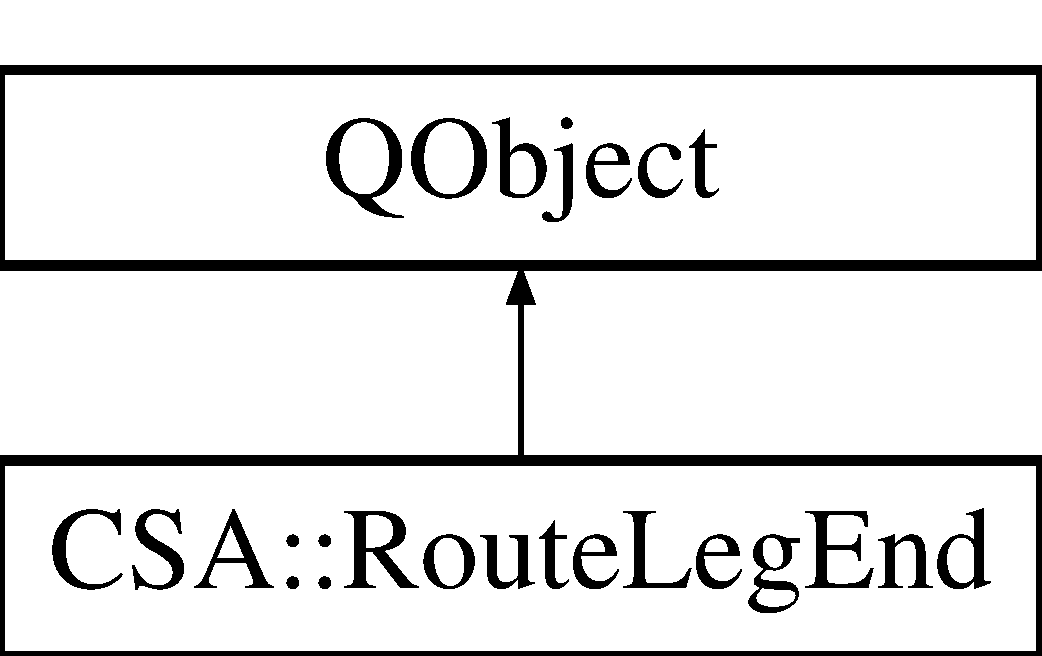
\includegraphics[height=2.000000cm]{classCSA_1_1RouteLegEnd}
\end{center}
\end{figure}
\subsection*{Signals}
\begin{DoxyCompactItemize}
\item 
void \mbox{\hyperlink{classCSA_1_1RouteLegEnd_a7b076ed1ca3388fc45fd7445a3e28fc6}{uri\+Changed}} ()
\item 
void \mbox{\hyperlink{classCSA_1_1RouteLegEnd_a3e72a28f87df8e3b87c8216faf183985}{time\+Changed}} ()
\item 
void \mbox{\hyperlink{classCSA_1_1RouteLegEnd_ad9cf094a7ca6cb658eef22745bccde12}{station\+Changed}} ()
\item 
void \mbox{\hyperlink{classCSA_1_1RouteLegEnd_a5ac2ad71e228b4f525d6a63f55c62b6f}{platform\+Changed}} ()
\item 
void \mbox{\hyperlink{classCSA_1_1RouteLegEnd_ae84dbef16916f8a23b528906620b628f}{is\+Normal\+Platform\+Changed}} ()
\item 
void \mbox{\hyperlink{classCSA_1_1RouteLegEnd_a68c581c134a26e25daf080d393b0ff76}{delay\+Changed}} ()
\item 
void \mbox{\hyperlink{classCSA_1_1RouteLegEnd_aa11ab3e90ebb2e920b2a0b0517871f73}{is\+Canceled\+Changed}} ()
\item 
void \mbox{\hyperlink{classCSA_1_1RouteLegEnd_a2af1d9d5f71a85c19790b356fdfe0c33}{is\+Passed\+Changed}} ()
\item 
void \mbox{\hyperlink{classCSA_1_1RouteLegEnd_a192aa2d98e40a2f19fa332fe3a65efac}{occupancy\+Level\+Changed}} ()
\end{DoxyCompactItemize}
\subsection*{Public Member Functions}
\begin{DoxyCompactItemize}
\item 
\mbox{\hyperlink{classCSA_1_1RouteLegEnd_a209849fda86c0e85e7c5b6b740471679}{Route\+Leg\+End}} (const Q\+Url \&\mbox{\hyperlink{classCSA_1_1RouteLegEnd_a6461241e58c65d43279afca09fd6be8a}{uri}}, const Q\+Date\+Time \&\mbox{\hyperlink{classCSA_1_1RouteLegEnd_af4543d06eb45cb23ef27d76f75a34ba7}{time}}, \mbox{\hyperlink{classCSA_1_1Station}{C\+S\+A\+::\+Station}} $\ast$\mbox{\hyperlink{classCSA_1_1RouteLegEnd_af8401206d340ff819ccc77dbc9b04c4b}{station}}, const Q\+String \&\mbox{\hyperlink{classCSA_1_1RouteLegEnd_a3ae0babc5849e36e2df61410da6a1cdd}{platform}}, const bool \&\mbox{\hyperlink{classCSA_1_1RouteLegEnd_a516ce67088e866a951fde382dba4e9e2}{is\+Normal\+Platform}}, const qint16 \&\mbox{\hyperlink{classCSA_1_1RouteLegEnd_ab1ea8c249d0a40884f446639ab030bc3}{delay}}, const bool \&\mbox{\hyperlink{classCSA_1_1RouteLegEnd_aca61ef191ba822aaed436707da242ef3}{is\+Canceled}}, const bool \&\mbox{\hyperlink{classCSA_1_1RouteLegEnd_a5359a35f5b132be17444fe8d1090671f}{is\+Passed}}, const \mbox{\hyperlink{classCSA_1_1Vehicle_a331cc81107e5f0a8f37f894729dd9bda}{C\+S\+A\+::\+Vehicle\+::\+Occupancy\+Level}} \&\mbox{\hyperlink{classCSA_1_1RouteLegEnd_aec102317dd7705a8b62b4ec8ee08597f}{occupancy\+Level}}, Q\+Object $\ast$parent=nullptr)
\item 
Q\+Url \mbox{\hyperlink{classCSA_1_1RouteLegEnd_a6461241e58c65d43279afca09fd6be8a}{uri}} () const
\item 
void \mbox{\hyperlink{classCSA_1_1RouteLegEnd_a7d5b3ff4ed0d733bc53db77fbf12a69c}{set\+Uri}} (const Q\+Url \&\mbox{\hyperlink{classCSA_1_1RouteLegEnd_a6461241e58c65d43279afca09fd6be8a}{uri}})
\item 
Q\+Date\+Time \mbox{\hyperlink{classCSA_1_1RouteLegEnd_af4543d06eb45cb23ef27d76f75a34ba7}{time}} () const
\item 
void \mbox{\hyperlink{classCSA_1_1RouteLegEnd_a20536e6606c877bc94f6093f8a0a4f1a}{set\+Time}} (const Q\+Date\+Time \&\mbox{\hyperlink{classCSA_1_1RouteLegEnd_af4543d06eb45cb23ef27d76f75a34ba7}{time}})
\item 
\mbox{\hyperlink{classCSA_1_1Station}{C\+S\+A\+::\+Station}} $\ast$ \mbox{\hyperlink{classCSA_1_1RouteLegEnd_af8401206d340ff819ccc77dbc9b04c4b}{station}} () const
\item 
void \mbox{\hyperlink{classCSA_1_1RouteLegEnd_aad038e9175944c0a0b494cb8413f1bbc}{set\+Station}} (\mbox{\hyperlink{classCSA_1_1Station}{C\+S\+A\+::\+Station}} $\ast$\mbox{\hyperlink{classCSA_1_1RouteLegEnd_af8401206d340ff819ccc77dbc9b04c4b}{station}})
\item 
Q\+String \mbox{\hyperlink{classCSA_1_1RouteLegEnd_a3ae0babc5849e36e2df61410da6a1cdd}{platform}} () const
\item 
void \mbox{\hyperlink{classCSA_1_1RouteLegEnd_abe99ad7c60f04350b460f1029ae2691d}{set\+Platform}} (const Q\+String \&\mbox{\hyperlink{classCSA_1_1RouteLegEnd_a3ae0babc5849e36e2df61410da6a1cdd}{platform}})
\item 
bool \mbox{\hyperlink{classCSA_1_1RouteLegEnd_a516ce67088e866a951fde382dba4e9e2}{is\+Normal\+Platform}} () const
\item 
void \mbox{\hyperlink{classCSA_1_1RouteLegEnd_a4a566505d3fb26d072e94b47a8c798bc}{set\+Is\+Normal\+Platform}} (bool \mbox{\hyperlink{classCSA_1_1RouteLegEnd_a516ce67088e866a951fde382dba4e9e2}{is\+Normal\+Platform}})
\item 
qint16 \mbox{\hyperlink{classCSA_1_1RouteLegEnd_ab1ea8c249d0a40884f446639ab030bc3}{delay}} () const
\item 
void \mbox{\hyperlink{classCSA_1_1RouteLegEnd_a39d7483632dc0703029ba8ea93390a45}{set\+Delay}} (const qint16 \&\mbox{\hyperlink{classCSA_1_1RouteLegEnd_ab1ea8c249d0a40884f446639ab030bc3}{delay}})
\item 
bool \mbox{\hyperlink{classCSA_1_1RouteLegEnd_aca61ef191ba822aaed436707da242ef3}{is\+Canceled}} () const
\item 
void \mbox{\hyperlink{classCSA_1_1RouteLegEnd_a73d8392ad94a85d85784ef6916282713}{set\+Is\+Canceled}} (bool \mbox{\hyperlink{classCSA_1_1RouteLegEnd_aca61ef191ba822aaed436707da242ef3}{is\+Canceled}})
\item 
bool \mbox{\hyperlink{classCSA_1_1RouteLegEnd_a5359a35f5b132be17444fe8d1090671f}{is\+Passed}} () const
\item 
void \mbox{\hyperlink{classCSA_1_1RouteLegEnd_a2a279d3b89f1d5847cd4e8ec575b488f}{set\+Is\+Passed}} (bool \mbox{\hyperlink{classCSA_1_1RouteLegEnd_a5359a35f5b132be17444fe8d1090671f}{is\+Passed}})
\item 
\mbox{\hyperlink{classCSA_1_1Vehicle_a331cc81107e5f0a8f37f894729dd9bda}{C\+S\+A\+::\+Vehicle\+::\+Occupancy\+Level}} \mbox{\hyperlink{classCSA_1_1RouteLegEnd_aec102317dd7705a8b62b4ec8ee08597f}{occupancy\+Level}} () const
\item 
void \mbox{\hyperlink{classCSA_1_1RouteLegEnd_a78147d9dfa7d02060aea3f3d34e76eae}{set\+Occupancy\+Level}} (const \mbox{\hyperlink{classCSA_1_1Vehicle_a331cc81107e5f0a8f37f894729dd9bda}{C\+S\+A\+::\+Vehicle\+::\+Occupancy\+Level}} \&\mbox{\hyperlink{classCSA_1_1RouteLegEnd_aec102317dd7705a8b62b4ec8ee08597f}{occupancy\+Level}})
\end{DoxyCompactItemize}
\subsection*{Private Attributes}
\begin{DoxyCompactItemize}
\item 
Q\+Url \mbox{\hyperlink{classCSA_1_1RouteLegEnd_a83202a0b6715895126d9bf11a9315279}{m\+\_\+uri}}
\item 
Q\+Date\+Time \mbox{\hyperlink{classCSA_1_1RouteLegEnd_a7572b34abc0d4f550706fee4558345d3}{m\+\_\+time}}
\item 
\mbox{\hyperlink{classCSA_1_1Station}{C\+S\+A\+::\+Station}} $\ast$ \mbox{\hyperlink{classCSA_1_1RouteLegEnd_ade143e56b08c85418c7d9353b1c80288}{m\+\_\+station}}
\item 
Q\+String \mbox{\hyperlink{classCSA_1_1RouteLegEnd_aacea60490b5bf82eb303fdaa8d8ac709}{m\+\_\+platform}}
\item 
bool \mbox{\hyperlink{classCSA_1_1RouteLegEnd_a0abd8fa004d9f7959233463145be24f0}{m\+\_\+is\+Normal\+Platform}}
\item 
qint16 \mbox{\hyperlink{classCSA_1_1RouteLegEnd_a426fe66c5e08f15f4617d6fd6a436199}{m\+\_\+delay}}
\item 
bool \mbox{\hyperlink{classCSA_1_1RouteLegEnd_a4ab0c3a3c545b376825bc3925c5b173b}{m\+\_\+is\+Canceled}}
\item 
bool \mbox{\hyperlink{classCSA_1_1RouteLegEnd_a739016bc10cc838f486d1fa37436ed43}{m\+\_\+is\+Passed}}
\item 
\mbox{\hyperlink{classCSA_1_1Vehicle_a331cc81107e5f0a8f37f894729dd9bda}{C\+S\+A\+::\+Vehicle\+::\+Occupancy\+Level}} \mbox{\hyperlink{classCSA_1_1RouteLegEnd_add4c875dfb78e698999c16963e17ee41}{m\+\_\+occupancy\+Level}}
\end{DoxyCompactItemize}


\subsection{Constructor \& Destructor Documentation}
\mbox{\Hypertarget{classCSA_1_1RouteLegEnd_a209849fda86c0e85e7c5b6b740471679}\label{classCSA_1_1RouteLegEnd_a209849fda86c0e85e7c5b6b740471679}} 
\index{C\+S\+A\+::\+Route\+Leg\+End@{C\+S\+A\+::\+Route\+Leg\+End}!Route\+Leg\+End@{Route\+Leg\+End}}
\index{Route\+Leg\+End@{Route\+Leg\+End}!C\+S\+A\+::\+Route\+Leg\+End@{C\+S\+A\+::\+Route\+Leg\+End}}
\subsubsection{\texorpdfstring{Route\+Leg\+End()}{RouteLegEnd()}}
{\footnotesize\ttfamily C\+S\+A\+::\+Route\+Leg\+End\+::\+Route\+Leg\+End (\begin{DoxyParamCaption}\item[{const Q\+Url \&}]{uri,  }\item[{const Q\+Date\+Time \&}]{time,  }\item[{\mbox{\hyperlink{classCSA_1_1Station}{C\+S\+A\+::\+Station}} $\ast$}]{station,  }\item[{const Q\+String \&}]{platform,  }\item[{const bool \&}]{is\+Normal\+Platform,  }\item[{const qint16 \&}]{delay,  }\item[{const bool \&}]{is\+Canceled,  }\item[{const bool \&}]{is\+Passed,  }\item[{const \mbox{\hyperlink{classCSA_1_1Vehicle_a331cc81107e5f0a8f37f894729dd9bda}{C\+S\+A\+::\+Vehicle\+::\+Occupancy\+Level}} \&}]{occupancy\+Level,  }\item[{Q\+Object $\ast$}]{parent = {\ttfamily nullptr} }\end{DoxyParamCaption})\hspace{0.3cm}{\ttfamily [explicit]}}



\subsection{Member Function Documentation}
\mbox{\Hypertarget{classCSA_1_1RouteLegEnd_ab1ea8c249d0a40884f446639ab030bc3}\label{classCSA_1_1RouteLegEnd_ab1ea8c249d0a40884f446639ab030bc3}} 
\index{C\+S\+A\+::\+Route\+Leg\+End@{C\+S\+A\+::\+Route\+Leg\+End}!delay@{delay}}
\index{delay@{delay}!C\+S\+A\+::\+Route\+Leg\+End@{C\+S\+A\+::\+Route\+Leg\+End}}
\subsubsection{\texorpdfstring{delay()}{delay()}}
{\footnotesize\ttfamily qint16 C\+S\+A\+::\+Route\+Leg\+End\+::delay (\begin{DoxyParamCaption}{ }\end{DoxyParamCaption}) const}

\mbox{\Hypertarget{classCSA_1_1RouteLegEnd_a68c581c134a26e25daf080d393b0ff76}\label{classCSA_1_1RouteLegEnd_a68c581c134a26e25daf080d393b0ff76}} 
\index{C\+S\+A\+::\+Route\+Leg\+End@{C\+S\+A\+::\+Route\+Leg\+End}!delay\+Changed@{delay\+Changed}}
\index{delay\+Changed@{delay\+Changed}!C\+S\+A\+::\+Route\+Leg\+End@{C\+S\+A\+::\+Route\+Leg\+End}}
\subsubsection{\texorpdfstring{delay\+Changed}{delayChanged}}
{\footnotesize\ttfamily void C\+S\+A\+::\+Route\+Leg\+End\+::delay\+Changed (\begin{DoxyParamCaption}{ }\end{DoxyParamCaption})\hspace{0.3cm}{\ttfamily [signal]}}

\mbox{\Hypertarget{classCSA_1_1RouteLegEnd_aca61ef191ba822aaed436707da242ef3}\label{classCSA_1_1RouteLegEnd_aca61ef191ba822aaed436707da242ef3}} 
\index{C\+S\+A\+::\+Route\+Leg\+End@{C\+S\+A\+::\+Route\+Leg\+End}!is\+Canceled@{is\+Canceled}}
\index{is\+Canceled@{is\+Canceled}!C\+S\+A\+::\+Route\+Leg\+End@{C\+S\+A\+::\+Route\+Leg\+End}}
\subsubsection{\texorpdfstring{is\+Canceled()}{isCanceled()}}
{\footnotesize\ttfamily bool C\+S\+A\+::\+Route\+Leg\+End\+::is\+Canceled (\begin{DoxyParamCaption}{ }\end{DoxyParamCaption}) const}

\mbox{\Hypertarget{classCSA_1_1RouteLegEnd_aa11ab3e90ebb2e920b2a0b0517871f73}\label{classCSA_1_1RouteLegEnd_aa11ab3e90ebb2e920b2a0b0517871f73}} 
\index{C\+S\+A\+::\+Route\+Leg\+End@{C\+S\+A\+::\+Route\+Leg\+End}!is\+Canceled\+Changed@{is\+Canceled\+Changed}}
\index{is\+Canceled\+Changed@{is\+Canceled\+Changed}!C\+S\+A\+::\+Route\+Leg\+End@{C\+S\+A\+::\+Route\+Leg\+End}}
\subsubsection{\texorpdfstring{is\+Canceled\+Changed}{isCanceledChanged}}
{\footnotesize\ttfamily void C\+S\+A\+::\+Route\+Leg\+End\+::is\+Canceled\+Changed (\begin{DoxyParamCaption}{ }\end{DoxyParamCaption})\hspace{0.3cm}{\ttfamily [signal]}}

\mbox{\Hypertarget{classCSA_1_1RouteLegEnd_a516ce67088e866a951fde382dba4e9e2}\label{classCSA_1_1RouteLegEnd_a516ce67088e866a951fde382dba4e9e2}} 
\index{C\+S\+A\+::\+Route\+Leg\+End@{C\+S\+A\+::\+Route\+Leg\+End}!is\+Normal\+Platform@{is\+Normal\+Platform}}
\index{is\+Normal\+Platform@{is\+Normal\+Platform}!C\+S\+A\+::\+Route\+Leg\+End@{C\+S\+A\+::\+Route\+Leg\+End}}
\subsubsection{\texorpdfstring{is\+Normal\+Platform()}{isNormalPlatform()}}
{\footnotesize\ttfamily bool C\+S\+A\+::\+Route\+Leg\+End\+::is\+Normal\+Platform (\begin{DoxyParamCaption}{ }\end{DoxyParamCaption}) const}

\mbox{\Hypertarget{classCSA_1_1RouteLegEnd_ae84dbef16916f8a23b528906620b628f}\label{classCSA_1_1RouteLegEnd_ae84dbef16916f8a23b528906620b628f}} 
\index{C\+S\+A\+::\+Route\+Leg\+End@{C\+S\+A\+::\+Route\+Leg\+End}!is\+Normal\+Platform\+Changed@{is\+Normal\+Platform\+Changed}}
\index{is\+Normal\+Platform\+Changed@{is\+Normal\+Platform\+Changed}!C\+S\+A\+::\+Route\+Leg\+End@{C\+S\+A\+::\+Route\+Leg\+End}}
\subsubsection{\texorpdfstring{is\+Normal\+Platform\+Changed}{isNormalPlatformChanged}}
{\footnotesize\ttfamily void C\+S\+A\+::\+Route\+Leg\+End\+::is\+Normal\+Platform\+Changed (\begin{DoxyParamCaption}{ }\end{DoxyParamCaption})\hspace{0.3cm}{\ttfamily [signal]}}

\mbox{\Hypertarget{classCSA_1_1RouteLegEnd_a5359a35f5b132be17444fe8d1090671f}\label{classCSA_1_1RouteLegEnd_a5359a35f5b132be17444fe8d1090671f}} 
\index{C\+S\+A\+::\+Route\+Leg\+End@{C\+S\+A\+::\+Route\+Leg\+End}!is\+Passed@{is\+Passed}}
\index{is\+Passed@{is\+Passed}!C\+S\+A\+::\+Route\+Leg\+End@{C\+S\+A\+::\+Route\+Leg\+End}}
\subsubsection{\texorpdfstring{is\+Passed()}{isPassed()}}
{\footnotesize\ttfamily bool C\+S\+A\+::\+Route\+Leg\+End\+::is\+Passed (\begin{DoxyParamCaption}{ }\end{DoxyParamCaption}) const}

\mbox{\Hypertarget{classCSA_1_1RouteLegEnd_a2af1d9d5f71a85c19790b356fdfe0c33}\label{classCSA_1_1RouteLegEnd_a2af1d9d5f71a85c19790b356fdfe0c33}} 
\index{C\+S\+A\+::\+Route\+Leg\+End@{C\+S\+A\+::\+Route\+Leg\+End}!is\+Passed\+Changed@{is\+Passed\+Changed}}
\index{is\+Passed\+Changed@{is\+Passed\+Changed}!C\+S\+A\+::\+Route\+Leg\+End@{C\+S\+A\+::\+Route\+Leg\+End}}
\subsubsection{\texorpdfstring{is\+Passed\+Changed}{isPassedChanged}}
{\footnotesize\ttfamily void C\+S\+A\+::\+Route\+Leg\+End\+::is\+Passed\+Changed (\begin{DoxyParamCaption}{ }\end{DoxyParamCaption})\hspace{0.3cm}{\ttfamily [signal]}}

\mbox{\Hypertarget{classCSA_1_1RouteLegEnd_aec102317dd7705a8b62b4ec8ee08597f}\label{classCSA_1_1RouteLegEnd_aec102317dd7705a8b62b4ec8ee08597f}} 
\index{C\+S\+A\+::\+Route\+Leg\+End@{C\+S\+A\+::\+Route\+Leg\+End}!occupancy\+Level@{occupancy\+Level}}
\index{occupancy\+Level@{occupancy\+Level}!C\+S\+A\+::\+Route\+Leg\+End@{C\+S\+A\+::\+Route\+Leg\+End}}
\subsubsection{\texorpdfstring{occupancy\+Level()}{occupancyLevel()}}
{\footnotesize\ttfamily \mbox{\hyperlink{classCSA_1_1Vehicle_a331cc81107e5f0a8f37f894729dd9bda}{C\+S\+A\+::\+Vehicle\+::\+Occupancy\+Level}} C\+S\+A\+::\+Route\+Leg\+End\+::occupancy\+Level (\begin{DoxyParamCaption}{ }\end{DoxyParamCaption}) const}

\mbox{\Hypertarget{classCSA_1_1RouteLegEnd_a192aa2d98e40a2f19fa332fe3a65efac}\label{classCSA_1_1RouteLegEnd_a192aa2d98e40a2f19fa332fe3a65efac}} 
\index{C\+S\+A\+::\+Route\+Leg\+End@{C\+S\+A\+::\+Route\+Leg\+End}!occupancy\+Level\+Changed@{occupancy\+Level\+Changed}}
\index{occupancy\+Level\+Changed@{occupancy\+Level\+Changed}!C\+S\+A\+::\+Route\+Leg\+End@{C\+S\+A\+::\+Route\+Leg\+End}}
\subsubsection{\texorpdfstring{occupancy\+Level\+Changed}{occupancyLevelChanged}}
{\footnotesize\ttfamily void C\+S\+A\+::\+Route\+Leg\+End\+::occupancy\+Level\+Changed (\begin{DoxyParamCaption}{ }\end{DoxyParamCaption})\hspace{0.3cm}{\ttfamily [signal]}}

\mbox{\Hypertarget{classCSA_1_1RouteLegEnd_a3ae0babc5849e36e2df61410da6a1cdd}\label{classCSA_1_1RouteLegEnd_a3ae0babc5849e36e2df61410da6a1cdd}} 
\index{C\+S\+A\+::\+Route\+Leg\+End@{C\+S\+A\+::\+Route\+Leg\+End}!platform@{platform}}
\index{platform@{platform}!C\+S\+A\+::\+Route\+Leg\+End@{C\+S\+A\+::\+Route\+Leg\+End}}
\subsubsection{\texorpdfstring{platform()}{platform()}}
{\footnotesize\ttfamily Q\+String C\+S\+A\+::\+Route\+Leg\+End\+::platform (\begin{DoxyParamCaption}{ }\end{DoxyParamCaption}) const}

\mbox{\Hypertarget{classCSA_1_1RouteLegEnd_a5ac2ad71e228b4f525d6a63f55c62b6f}\label{classCSA_1_1RouteLegEnd_a5ac2ad71e228b4f525d6a63f55c62b6f}} 
\index{C\+S\+A\+::\+Route\+Leg\+End@{C\+S\+A\+::\+Route\+Leg\+End}!platform\+Changed@{platform\+Changed}}
\index{platform\+Changed@{platform\+Changed}!C\+S\+A\+::\+Route\+Leg\+End@{C\+S\+A\+::\+Route\+Leg\+End}}
\subsubsection{\texorpdfstring{platform\+Changed}{platformChanged}}
{\footnotesize\ttfamily void C\+S\+A\+::\+Route\+Leg\+End\+::platform\+Changed (\begin{DoxyParamCaption}{ }\end{DoxyParamCaption})\hspace{0.3cm}{\ttfamily [signal]}}

\mbox{\Hypertarget{classCSA_1_1RouteLegEnd_a39d7483632dc0703029ba8ea93390a45}\label{classCSA_1_1RouteLegEnd_a39d7483632dc0703029ba8ea93390a45}} 
\index{C\+S\+A\+::\+Route\+Leg\+End@{C\+S\+A\+::\+Route\+Leg\+End}!set\+Delay@{set\+Delay}}
\index{set\+Delay@{set\+Delay}!C\+S\+A\+::\+Route\+Leg\+End@{C\+S\+A\+::\+Route\+Leg\+End}}
\subsubsection{\texorpdfstring{set\+Delay()}{setDelay()}}
{\footnotesize\ttfamily void C\+S\+A\+::\+Route\+Leg\+End\+::set\+Delay (\begin{DoxyParamCaption}\item[{const qint16 \&}]{delay }\end{DoxyParamCaption})}

\mbox{\Hypertarget{classCSA_1_1RouteLegEnd_a73d8392ad94a85d85784ef6916282713}\label{classCSA_1_1RouteLegEnd_a73d8392ad94a85d85784ef6916282713}} 
\index{C\+S\+A\+::\+Route\+Leg\+End@{C\+S\+A\+::\+Route\+Leg\+End}!set\+Is\+Canceled@{set\+Is\+Canceled}}
\index{set\+Is\+Canceled@{set\+Is\+Canceled}!C\+S\+A\+::\+Route\+Leg\+End@{C\+S\+A\+::\+Route\+Leg\+End}}
\subsubsection{\texorpdfstring{set\+Is\+Canceled()}{setIsCanceled()}}
{\footnotesize\ttfamily void C\+S\+A\+::\+Route\+Leg\+End\+::set\+Is\+Canceled (\begin{DoxyParamCaption}\item[{bool}]{is\+Canceled }\end{DoxyParamCaption})}

\mbox{\Hypertarget{classCSA_1_1RouteLegEnd_a4a566505d3fb26d072e94b47a8c798bc}\label{classCSA_1_1RouteLegEnd_a4a566505d3fb26d072e94b47a8c798bc}} 
\index{C\+S\+A\+::\+Route\+Leg\+End@{C\+S\+A\+::\+Route\+Leg\+End}!set\+Is\+Normal\+Platform@{set\+Is\+Normal\+Platform}}
\index{set\+Is\+Normal\+Platform@{set\+Is\+Normal\+Platform}!C\+S\+A\+::\+Route\+Leg\+End@{C\+S\+A\+::\+Route\+Leg\+End}}
\subsubsection{\texorpdfstring{set\+Is\+Normal\+Platform()}{setIsNormalPlatform()}}
{\footnotesize\ttfamily void C\+S\+A\+::\+Route\+Leg\+End\+::set\+Is\+Normal\+Platform (\begin{DoxyParamCaption}\item[{bool}]{is\+Normal\+Platform }\end{DoxyParamCaption})}

\mbox{\Hypertarget{classCSA_1_1RouteLegEnd_a2a279d3b89f1d5847cd4e8ec575b488f}\label{classCSA_1_1RouteLegEnd_a2a279d3b89f1d5847cd4e8ec575b488f}} 
\index{C\+S\+A\+::\+Route\+Leg\+End@{C\+S\+A\+::\+Route\+Leg\+End}!set\+Is\+Passed@{set\+Is\+Passed}}
\index{set\+Is\+Passed@{set\+Is\+Passed}!C\+S\+A\+::\+Route\+Leg\+End@{C\+S\+A\+::\+Route\+Leg\+End}}
\subsubsection{\texorpdfstring{set\+Is\+Passed()}{setIsPassed()}}
{\footnotesize\ttfamily void C\+S\+A\+::\+Route\+Leg\+End\+::set\+Is\+Passed (\begin{DoxyParamCaption}\item[{bool}]{is\+Passed }\end{DoxyParamCaption})}

\mbox{\Hypertarget{classCSA_1_1RouteLegEnd_a78147d9dfa7d02060aea3f3d34e76eae}\label{classCSA_1_1RouteLegEnd_a78147d9dfa7d02060aea3f3d34e76eae}} 
\index{C\+S\+A\+::\+Route\+Leg\+End@{C\+S\+A\+::\+Route\+Leg\+End}!set\+Occupancy\+Level@{set\+Occupancy\+Level}}
\index{set\+Occupancy\+Level@{set\+Occupancy\+Level}!C\+S\+A\+::\+Route\+Leg\+End@{C\+S\+A\+::\+Route\+Leg\+End}}
\subsubsection{\texorpdfstring{set\+Occupancy\+Level()}{setOccupancyLevel()}}
{\footnotesize\ttfamily void C\+S\+A\+::\+Route\+Leg\+End\+::set\+Occupancy\+Level (\begin{DoxyParamCaption}\item[{const \mbox{\hyperlink{classCSA_1_1Vehicle_a331cc81107e5f0a8f37f894729dd9bda}{C\+S\+A\+::\+Vehicle\+::\+Occupancy\+Level}} \&}]{occupancy\+Level }\end{DoxyParamCaption})}

\mbox{\Hypertarget{classCSA_1_1RouteLegEnd_abe99ad7c60f04350b460f1029ae2691d}\label{classCSA_1_1RouteLegEnd_abe99ad7c60f04350b460f1029ae2691d}} 
\index{C\+S\+A\+::\+Route\+Leg\+End@{C\+S\+A\+::\+Route\+Leg\+End}!set\+Platform@{set\+Platform}}
\index{set\+Platform@{set\+Platform}!C\+S\+A\+::\+Route\+Leg\+End@{C\+S\+A\+::\+Route\+Leg\+End}}
\subsubsection{\texorpdfstring{set\+Platform()}{setPlatform()}}
{\footnotesize\ttfamily void C\+S\+A\+::\+Route\+Leg\+End\+::set\+Platform (\begin{DoxyParamCaption}\item[{const Q\+String \&}]{platform }\end{DoxyParamCaption})}

\mbox{\Hypertarget{classCSA_1_1RouteLegEnd_aad038e9175944c0a0b494cb8413f1bbc}\label{classCSA_1_1RouteLegEnd_aad038e9175944c0a0b494cb8413f1bbc}} 
\index{C\+S\+A\+::\+Route\+Leg\+End@{C\+S\+A\+::\+Route\+Leg\+End}!set\+Station@{set\+Station}}
\index{set\+Station@{set\+Station}!C\+S\+A\+::\+Route\+Leg\+End@{C\+S\+A\+::\+Route\+Leg\+End}}
\subsubsection{\texorpdfstring{set\+Station()}{setStation()}}
{\footnotesize\ttfamily void C\+S\+A\+::\+Route\+Leg\+End\+::set\+Station (\begin{DoxyParamCaption}\item[{\mbox{\hyperlink{classCSA_1_1Station}{C\+S\+A\+::\+Station}} $\ast$}]{station }\end{DoxyParamCaption})}

\mbox{\Hypertarget{classCSA_1_1RouteLegEnd_a20536e6606c877bc94f6093f8a0a4f1a}\label{classCSA_1_1RouteLegEnd_a20536e6606c877bc94f6093f8a0a4f1a}} 
\index{C\+S\+A\+::\+Route\+Leg\+End@{C\+S\+A\+::\+Route\+Leg\+End}!set\+Time@{set\+Time}}
\index{set\+Time@{set\+Time}!C\+S\+A\+::\+Route\+Leg\+End@{C\+S\+A\+::\+Route\+Leg\+End}}
\subsubsection{\texorpdfstring{set\+Time()}{setTime()}}
{\footnotesize\ttfamily void C\+S\+A\+::\+Route\+Leg\+End\+::set\+Time (\begin{DoxyParamCaption}\item[{const Q\+Date\+Time \&}]{time }\end{DoxyParamCaption})}

\mbox{\Hypertarget{classCSA_1_1RouteLegEnd_a7d5b3ff4ed0d733bc53db77fbf12a69c}\label{classCSA_1_1RouteLegEnd_a7d5b3ff4ed0d733bc53db77fbf12a69c}} 
\index{C\+S\+A\+::\+Route\+Leg\+End@{C\+S\+A\+::\+Route\+Leg\+End}!set\+Uri@{set\+Uri}}
\index{set\+Uri@{set\+Uri}!C\+S\+A\+::\+Route\+Leg\+End@{C\+S\+A\+::\+Route\+Leg\+End}}
\subsubsection{\texorpdfstring{set\+Uri()}{setUri()}}
{\footnotesize\ttfamily void C\+S\+A\+::\+Route\+Leg\+End\+::set\+Uri (\begin{DoxyParamCaption}\item[{const Q\+Url \&}]{uri }\end{DoxyParamCaption})}

\mbox{\Hypertarget{classCSA_1_1RouteLegEnd_af8401206d340ff819ccc77dbc9b04c4b}\label{classCSA_1_1RouteLegEnd_af8401206d340ff819ccc77dbc9b04c4b}} 
\index{C\+S\+A\+::\+Route\+Leg\+End@{C\+S\+A\+::\+Route\+Leg\+End}!station@{station}}
\index{station@{station}!C\+S\+A\+::\+Route\+Leg\+End@{C\+S\+A\+::\+Route\+Leg\+End}}
\subsubsection{\texorpdfstring{station()}{station()}}
{\footnotesize\ttfamily \mbox{\hyperlink{classCSA_1_1Station}{C\+S\+A\+::\+Station}} $\ast$ C\+S\+A\+::\+Route\+Leg\+End\+::station (\begin{DoxyParamCaption}{ }\end{DoxyParamCaption}) const}

\mbox{\Hypertarget{classCSA_1_1RouteLegEnd_ad9cf094a7ca6cb658eef22745bccde12}\label{classCSA_1_1RouteLegEnd_ad9cf094a7ca6cb658eef22745bccde12}} 
\index{C\+S\+A\+::\+Route\+Leg\+End@{C\+S\+A\+::\+Route\+Leg\+End}!station\+Changed@{station\+Changed}}
\index{station\+Changed@{station\+Changed}!C\+S\+A\+::\+Route\+Leg\+End@{C\+S\+A\+::\+Route\+Leg\+End}}
\subsubsection{\texorpdfstring{station\+Changed}{stationChanged}}
{\footnotesize\ttfamily void C\+S\+A\+::\+Route\+Leg\+End\+::station\+Changed (\begin{DoxyParamCaption}{ }\end{DoxyParamCaption})\hspace{0.3cm}{\ttfamily [signal]}}

\mbox{\Hypertarget{classCSA_1_1RouteLegEnd_af4543d06eb45cb23ef27d76f75a34ba7}\label{classCSA_1_1RouteLegEnd_af4543d06eb45cb23ef27d76f75a34ba7}} 
\index{C\+S\+A\+::\+Route\+Leg\+End@{C\+S\+A\+::\+Route\+Leg\+End}!time@{time}}
\index{time@{time}!C\+S\+A\+::\+Route\+Leg\+End@{C\+S\+A\+::\+Route\+Leg\+End}}
\subsubsection{\texorpdfstring{time()}{time()}}
{\footnotesize\ttfamily Q\+Date\+Time C\+S\+A\+::\+Route\+Leg\+End\+::time (\begin{DoxyParamCaption}{ }\end{DoxyParamCaption}) const}

\mbox{\Hypertarget{classCSA_1_1RouteLegEnd_a3e72a28f87df8e3b87c8216faf183985}\label{classCSA_1_1RouteLegEnd_a3e72a28f87df8e3b87c8216faf183985}} 
\index{C\+S\+A\+::\+Route\+Leg\+End@{C\+S\+A\+::\+Route\+Leg\+End}!time\+Changed@{time\+Changed}}
\index{time\+Changed@{time\+Changed}!C\+S\+A\+::\+Route\+Leg\+End@{C\+S\+A\+::\+Route\+Leg\+End}}
\subsubsection{\texorpdfstring{time\+Changed}{timeChanged}}
{\footnotesize\ttfamily void C\+S\+A\+::\+Route\+Leg\+End\+::time\+Changed (\begin{DoxyParamCaption}{ }\end{DoxyParamCaption})\hspace{0.3cm}{\ttfamily [signal]}}

\mbox{\Hypertarget{classCSA_1_1RouteLegEnd_a6461241e58c65d43279afca09fd6be8a}\label{classCSA_1_1RouteLegEnd_a6461241e58c65d43279afca09fd6be8a}} 
\index{C\+S\+A\+::\+Route\+Leg\+End@{C\+S\+A\+::\+Route\+Leg\+End}!uri@{uri}}
\index{uri@{uri}!C\+S\+A\+::\+Route\+Leg\+End@{C\+S\+A\+::\+Route\+Leg\+End}}
\subsubsection{\texorpdfstring{uri()}{uri()}}
{\footnotesize\ttfamily Q\+Url C\+S\+A\+::\+Route\+Leg\+End\+::uri (\begin{DoxyParamCaption}{ }\end{DoxyParamCaption}) const}

\mbox{\Hypertarget{classCSA_1_1RouteLegEnd_a7b076ed1ca3388fc45fd7445a3e28fc6}\label{classCSA_1_1RouteLegEnd_a7b076ed1ca3388fc45fd7445a3e28fc6}} 
\index{C\+S\+A\+::\+Route\+Leg\+End@{C\+S\+A\+::\+Route\+Leg\+End}!uri\+Changed@{uri\+Changed}}
\index{uri\+Changed@{uri\+Changed}!C\+S\+A\+::\+Route\+Leg\+End@{C\+S\+A\+::\+Route\+Leg\+End}}
\subsubsection{\texorpdfstring{uri\+Changed}{uriChanged}}
{\footnotesize\ttfamily void C\+S\+A\+::\+Route\+Leg\+End\+::uri\+Changed (\begin{DoxyParamCaption}{ }\end{DoxyParamCaption})\hspace{0.3cm}{\ttfamily [signal]}}



\subsection{Member Data Documentation}
\mbox{\Hypertarget{classCSA_1_1RouteLegEnd_a426fe66c5e08f15f4617d6fd6a436199}\label{classCSA_1_1RouteLegEnd_a426fe66c5e08f15f4617d6fd6a436199}} 
\index{C\+S\+A\+::\+Route\+Leg\+End@{C\+S\+A\+::\+Route\+Leg\+End}!m\+\_\+delay@{m\+\_\+delay}}
\index{m\+\_\+delay@{m\+\_\+delay}!C\+S\+A\+::\+Route\+Leg\+End@{C\+S\+A\+::\+Route\+Leg\+End}}
\subsubsection{\texorpdfstring{m\+\_\+delay}{m\_delay}}
{\footnotesize\ttfamily qint16 C\+S\+A\+::\+Route\+Leg\+End\+::m\+\_\+delay\hspace{0.3cm}{\ttfamily [private]}}

\mbox{\Hypertarget{classCSA_1_1RouteLegEnd_a4ab0c3a3c545b376825bc3925c5b173b}\label{classCSA_1_1RouteLegEnd_a4ab0c3a3c545b376825bc3925c5b173b}} 
\index{C\+S\+A\+::\+Route\+Leg\+End@{C\+S\+A\+::\+Route\+Leg\+End}!m\+\_\+is\+Canceled@{m\+\_\+is\+Canceled}}
\index{m\+\_\+is\+Canceled@{m\+\_\+is\+Canceled}!C\+S\+A\+::\+Route\+Leg\+End@{C\+S\+A\+::\+Route\+Leg\+End}}
\subsubsection{\texorpdfstring{m\+\_\+is\+Canceled}{m\_isCanceled}}
{\footnotesize\ttfamily bool C\+S\+A\+::\+Route\+Leg\+End\+::m\+\_\+is\+Canceled\hspace{0.3cm}{\ttfamily [private]}}

\mbox{\Hypertarget{classCSA_1_1RouteLegEnd_a0abd8fa004d9f7959233463145be24f0}\label{classCSA_1_1RouteLegEnd_a0abd8fa004d9f7959233463145be24f0}} 
\index{C\+S\+A\+::\+Route\+Leg\+End@{C\+S\+A\+::\+Route\+Leg\+End}!m\+\_\+is\+Normal\+Platform@{m\+\_\+is\+Normal\+Platform}}
\index{m\+\_\+is\+Normal\+Platform@{m\+\_\+is\+Normal\+Platform}!C\+S\+A\+::\+Route\+Leg\+End@{C\+S\+A\+::\+Route\+Leg\+End}}
\subsubsection{\texorpdfstring{m\+\_\+is\+Normal\+Platform}{m\_isNormalPlatform}}
{\footnotesize\ttfamily bool C\+S\+A\+::\+Route\+Leg\+End\+::m\+\_\+is\+Normal\+Platform\hspace{0.3cm}{\ttfamily [private]}}

\mbox{\Hypertarget{classCSA_1_1RouteLegEnd_a739016bc10cc838f486d1fa37436ed43}\label{classCSA_1_1RouteLegEnd_a739016bc10cc838f486d1fa37436ed43}} 
\index{C\+S\+A\+::\+Route\+Leg\+End@{C\+S\+A\+::\+Route\+Leg\+End}!m\+\_\+is\+Passed@{m\+\_\+is\+Passed}}
\index{m\+\_\+is\+Passed@{m\+\_\+is\+Passed}!C\+S\+A\+::\+Route\+Leg\+End@{C\+S\+A\+::\+Route\+Leg\+End}}
\subsubsection{\texorpdfstring{m\+\_\+is\+Passed}{m\_isPassed}}
{\footnotesize\ttfamily bool C\+S\+A\+::\+Route\+Leg\+End\+::m\+\_\+is\+Passed\hspace{0.3cm}{\ttfamily [private]}}

\mbox{\Hypertarget{classCSA_1_1RouteLegEnd_add4c875dfb78e698999c16963e17ee41}\label{classCSA_1_1RouteLegEnd_add4c875dfb78e698999c16963e17ee41}} 
\index{C\+S\+A\+::\+Route\+Leg\+End@{C\+S\+A\+::\+Route\+Leg\+End}!m\+\_\+occupancy\+Level@{m\+\_\+occupancy\+Level}}
\index{m\+\_\+occupancy\+Level@{m\+\_\+occupancy\+Level}!C\+S\+A\+::\+Route\+Leg\+End@{C\+S\+A\+::\+Route\+Leg\+End}}
\subsubsection{\texorpdfstring{m\+\_\+occupancy\+Level}{m\_occupancyLevel}}
{\footnotesize\ttfamily \mbox{\hyperlink{classCSA_1_1Vehicle_a331cc81107e5f0a8f37f894729dd9bda}{C\+S\+A\+::\+Vehicle\+::\+Occupancy\+Level}} C\+S\+A\+::\+Route\+Leg\+End\+::m\+\_\+occupancy\+Level\hspace{0.3cm}{\ttfamily [private]}}

\mbox{\Hypertarget{classCSA_1_1RouteLegEnd_aacea60490b5bf82eb303fdaa8d8ac709}\label{classCSA_1_1RouteLegEnd_aacea60490b5bf82eb303fdaa8d8ac709}} 
\index{C\+S\+A\+::\+Route\+Leg\+End@{C\+S\+A\+::\+Route\+Leg\+End}!m\+\_\+platform@{m\+\_\+platform}}
\index{m\+\_\+platform@{m\+\_\+platform}!C\+S\+A\+::\+Route\+Leg\+End@{C\+S\+A\+::\+Route\+Leg\+End}}
\subsubsection{\texorpdfstring{m\+\_\+platform}{m\_platform}}
{\footnotesize\ttfamily Q\+String C\+S\+A\+::\+Route\+Leg\+End\+::m\+\_\+platform\hspace{0.3cm}{\ttfamily [private]}}

\mbox{\Hypertarget{classCSA_1_1RouteLegEnd_ade143e56b08c85418c7d9353b1c80288}\label{classCSA_1_1RouteLegEnd_ade143e56b08c85418c7d9353b1c80288}} 
\index{C\+S\+A\+::\+Route\+Leg\+End@{C\+S\+A\+::\+Route\+Leg\+End}!m\+\_\+station@{m\+\_\+station}}
\index{m\+\_\+station@{m\+\_\+station}!C\+S\+A\+::\+Route\+Leg\+End@{C\+S\+A\+::\+Route\+Leg\+End}}
\subsubsection{\texorpdfstring{m\+\_\+station}{m\_station}}
{\footnotesize\ttfamily \mbox{\hyperlink{classCSA_1_1Station}{C\+S\+A\+::\+Station}}$\ast$ C\+S\+A\+::\+Route\+Leg\+End\+::m\+\_\+station\hspace{0.3cm}{\ttfamily [private]}}

\mbox{\Hypertarget{classCSA_1_1RouteLegEnd_a7572b34abc0d4f550706fee4558345d3}\label{classCSA_1_1RouteLegEnd_a7572b34abc0d4f550706fee4558345d3}} 
\index{C\+S\+A\+::\+Route\+Leg\+End@{C\+S\+A\+::\+Route\+Leg\+End}!m\+\_\+time@{m\+\_\+time}}
\index{m\+\_\+time@{m\+\_\+time}!C\+S\+A\+::\+Route\+Leg\+End@{C\+S\+A\+::\+Route\+Leg\+End}}
\subsubsection{\texorpdfstring{m\+\_\+time}{m\_time}}
{\footnotesize\ttfamily Q\+Date\+Time C\+S\+A\+::\+Route\+Leg\+End\+::m\+\_\+time\hspace{0.3cm}{\ttfamily [private]}}

\mbox{\Hypertarget{classCSA_1_1RouteLegEnd_a83202a0b6715895126d9bf11a9315279}\label{classCSA_1_1RouteLegEnd_a83202a0b6715895126d9bf11a9315279}} 
\index{C\+S\+A\+::\+Route\+Leg\+End@{C\+S\+A\+::\+Route\+Leg\+End}!m\+\_\+uri@{m\+\_\+uri}}
\index{m\+\_\+uri@{m\+\_\+uri}!C\+S\+A\+::\+Route\+Leg\+End@{C\+S\+A\+::\+Route\+Leg\+End}}
\subsubsection{\texorpdfstring{m\+\_\+uri}{m\_uri}}
{\footnotesize\ttfamily Q\+Url C\+S\+A\+::\+Route\+Leg\+End\+::m\+\_\+uri\hspace{0.3cm}{\ttfamily [private]}}



The documentation for this class was generated from the following files\+:\begin{DoxyCompactItemize}
\item 
src/linkedconnections/csa/\mbox{\hyperlink{csaroutelegend_8h}{csaroutelegend.\+h}}\item 
src/linkedconnections/csa/\mbox{\hyperlink{csaroutelegend_8cpp}{csaroutelegend.\+cpp}}\end{DoxyCompactItemize}

\hypertarget{classCSA_1_1Station}{}\section{C\+SA\+:\+:Station Class Reference}
\label{classCSA_1_1Station}\index{C\+S\+A\+::\+Station@{C\+S\+A\+::\+Station}}


{\ttfamily \#include $<$csastation.\+h$>$}

Inheritance diagram for C\+SA\+:\+:Station\+:\begin{figure}[H]
\begin{center}
\leavevmode
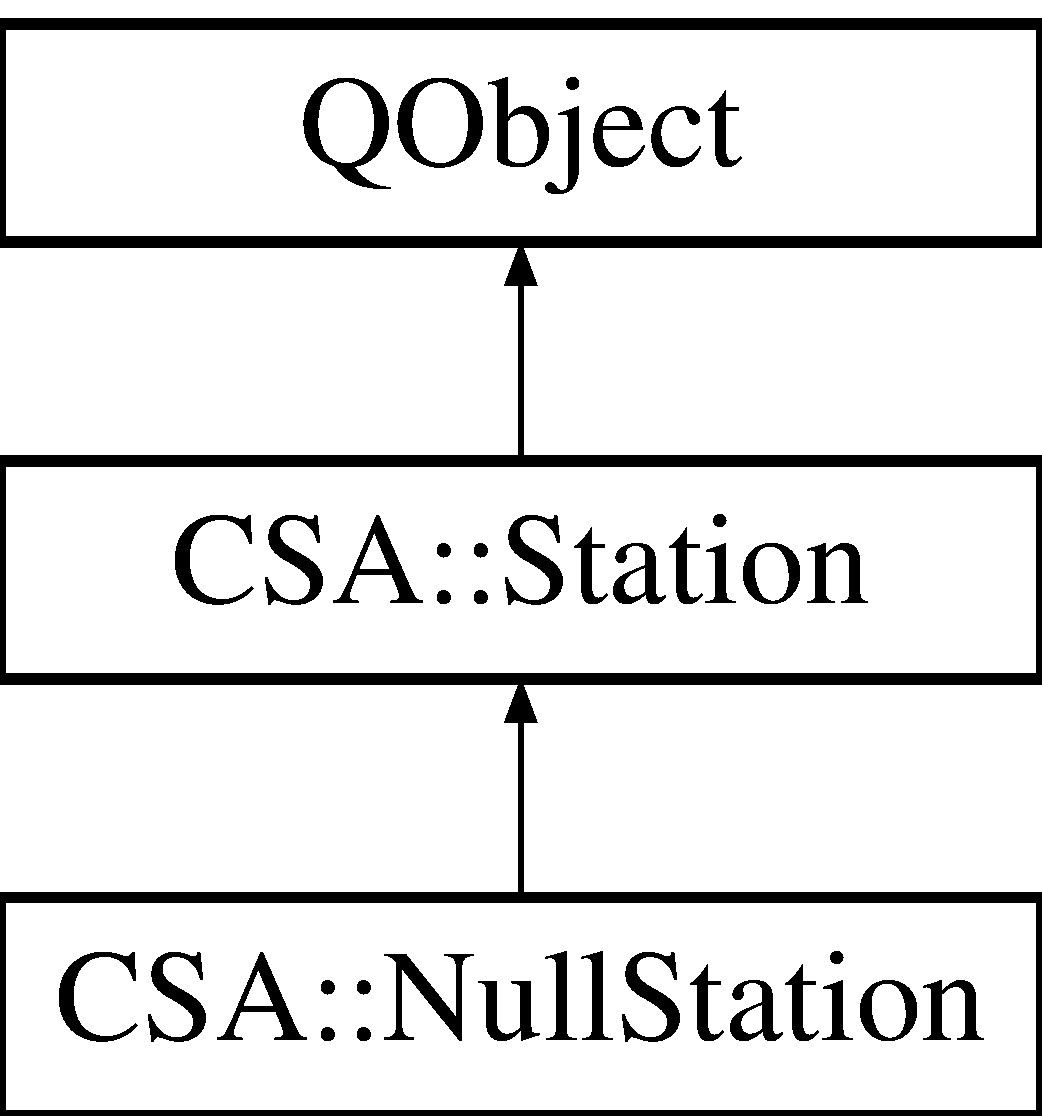
\includegraphics[height=3.000000cm]{classCSA_1_1Station}
\end{center}
\end{figure}
\subsection*{Public Types}
\begin{DoxyCompactItemize}
\item 
enum \mbox{\hyperlink{classCSA_1_1Station_aa160d0de40db0583099b5986dea1cd67}{Day}} \{ \newline
\mbox{\hyperlink{classCSA_1_1Station_aa160d0de40db0583099b5986dea1cd67a98617021b249af0ace0f84ee92ccc7cd}{Day\+::\+M\+O\+N\+D\+AY}}, 
\mbox{\hyperlink{classCSA_1_1Station_aa160d0de40db0583099b5986dea1cd67a5f5140afce13197a89e848004f292f14}{Day\+::\+T\+U\+E\+S\+D\+AY}}, 
\mbox{\hyperlink{classCSA_1_1Station_aa160d0de40db0583099b5986dea1cd67aaaebdc947e9f7d4ea362e5dc4fe7f825}{Day\+::\+W\+E\+D\+N\+E\+S\+D\+AY}}, 
\mbox{\hyperlink{classCSA_1_1Station_aa160d0de40db0583099b5986dea1cd67a7a61b324afb4dd8b2fb4a38afc34f755}{Day\+::\+T\+H\+U\+R\+S\+D\+AY}}, 
\newline
\mbox{\hyperlink{classCSA_1_1Station_aa160d0de40db0583099b5986dea1cd67a86fb6d343289267f3e9edb9b7403d936}{Day\+::\+F\+R\+I\+D\+AY}}, 
\mbox{\hyperlink{classCSA_1_1Station_aa160d0de40db0583099b5986dea1cd67afd5ae113ac00b67f69541bc8c7f21ef7}{Day\+::\+S\+A\+T\+U\+R\+D\+AY}}, 
\mbox{\hyperlink{classCSA_1_1Station_aa160d0de40db0583099b5986dea1cd67a95fa12cb2100ce7081b71f7c44bc12a5}{Day\+::\+S\+U\+N\+D\+AY}}
 \}
\end{DoxyCompactItemize}
\subsection*{Signals}
\begin{DoxyCompactItemize}
\item 
void \mbox{\hyperlink{classCSA_1_1Station_a7e1a832bc1ecff5811df303f907e9e04}{uri\+Changed}} ()
\item 
void \mbox{\hyperlink{classCSA_1_1Station_a86679a79fbe6a84b9890fcb15b5caa5e}{name\+Changed}} ()
\item 
void \mbox{\hyperlink{classCSA_1_1Station_ae7225d37accec94cf815e977b76109df}{country\+Changed}} ()
\item 
void \mbox{\hyperlink{classCSA_1_1Station_aceeec2e80a0a991acb3b74c539769bd8}{position\+Changed}} ()
\item 
void \mbox{\hyperlink{classCSA_1_1Station_a3d5070aa6b5fdb6adc893a51a0a1be2d}{address\+Changed}} ()
\item 
void \mbox{\hyperlink{classCSA_1_1Station_a269399db17611ed21b9a768cdc49159c}{has\+Ticket\+Vending\+Machine\+Changed}} ()
\item 
void \mbox{\hyperlink{classCSA_1_1Station_ad5cb28f158877e9c6f808bdc8a3b673c}{has\+Luggage\+Lockers\+Changed}} ()
\item 
void \mbox{\hyperlink{classCSA_1_1Station_af221724a180a08b013aae387a4234b41}{has\+Free\+Parking\+Changed}} ()
\item 
void \mbox{\hyperlink{classCSA_1_1Station_a06c0a1439cc5bfcbe8e065842f17f800}{has\+Taxi\+Changed}} ()
\item 
void \mbox{\hyperlink{classCSA_1_1Station_a2a974d267038288ae10200962f84eba5}{has\+Bicylce\+Spots\+Changed}} ()
\item 
void \mbox{\hyperlink{classCSA_1_1Station_a87ad9a5b8c69aca367ed1a5d65616ddb}{has\+Blue\+Bike\+Changed}} ()
\item 
void \mbox{\hyperlink{classCSA_1_1Station_a23a60c0e5b98f15e68d6fb71ee3bdd56}{has\+Bus\+Changed}} ()
\item 
void \mbox{\hyperlink{classCSA_1_1Station_ad997e9362b40f0f932e1a5d280dd42dc}{has\+Tram\+Changed}} ()
\item 
void \mbox{\hyperlink{classCSA_1_1Station_a1f006709983169db5059954aaeb868a4}{has\+Metro\+Changed}} ()
\item 
void \mbox{\hyperlink{classCSA_1_1Station_ad00b74e9cd7820e5f54a46efc006ff6a}{has\+Wheelchair\+Available\+Changed}} ()
\item 
void \mbox{\hyperlink{classCSA_1_1Station_a66bd1b6a58cd065fce51c8448019eab1}{has\+Ramp\+Changed}} ()
\item 
void \mbox{\hyperlink{classCSA_1_1Station_ad47a8ed217f646cce8661181dd4abcb8}{disabled\+Parking\+Spots\+Changed}} ()
\item 
void \mbox{\hyperlink{classCSA_1_1Station_a691c6d02127421821b41cfb40381781c}{has\+Elevated\+Platform\+Changed}} ()
\item 
void \mbox{\hyperlink{classCSA_1_1Station_a281adc596cffb53280beb8276ce9b0c5}{has\+Escalator\+Up\+Changed}} ()
\item 
void \mbox{\hyperlink{classCSA_1_1Station_a10898e5f4146f47f734c19708f614361}{has\+Escalator\+Down\+Changed}} ()
\item 
void \mbox{\hyperlink{classCSA_1_1Station_a21cce284fffaf5d90806c87eb827e021}{has\+Hearing\+Aid\+Signal\+Changed}} ()
\item 
void \mbox{\hyperlink{classCSA_1_1Station_a3f709e2a3661ed162d888aebff54144f}{opening\+Hours\+Changed}} ()
\item 
void \mbox{\hyperlink{classCSA_1_1Station_a96d22182cdb97e5c6ebe8468ffd5d8e7}{average\+Stop\+Times\+Changed}} ()
\end{DoxyCompactItemize}
\subsection*{Public Member Functions}
\begin{DoxyCompactItemize}
\item 
\mbox{\hyperlink{classCSA_1_1Station_a1ad546688826ab32a6451de33a5f20ca}{Station}} (Q\+Object $\ast$parent=nullptr)
\item 
\mbox{\hyperlink{classCSA_1_1Station_ab3703dee8550b5b6b72b83f4bc09cddc}{Station}} (const Q\+Url \&\mbox{\hyperlink{classCSA_1_1Station_addca2c54d5e9ce61c4ef9c3ee9ff4100}{uri}}, const Q\+Map$<$ Q\+Locale\+::\+Language, Q\+String $>$ \&\mbox{\hyperlink{classCSA_1_1Station_ad4442763fc108cde8368260119c007da}{name}}, const Q\+Locale\+::\+Country \&\mbox{\hyperlink{classCSA_1_1Station_ac54cea5fde8ba6e2367f0317965d9147}{country}}, const Q\+Geo\+Coordinate \&\mbox{\hyperlink{classCSA_1_1Station_a94249de9cc38d704eb6e77aca24daaea}{position}}, const qreal \&\mbox{\hyperlink{classCSA_1_1Station_aa8f1c3bfa7b4a3ad9ccc805ff7a2b931}{average\+Stop\+Times}}, Q\+Object $\ast$parent=nullptr)
\item 
\mbox{\hyperlink{classCSA_1_1Station_a2f28ea537ee63de36ef8b10ef4b17826}{Station}} (const Q\+Url \&\mbox{\hyperlink{classCSA_1_1Station_addca2c54d5e9ce61c4ef9c3ee9ff4100}{uri}}, const Q\+Map$<$ Q\+Locale\+::\+Language, Q\+String $>$ \&\mbox{\hyperlink{classCSA_1_1Station_ad4442763fc108cde8368260119c007da}{name}}, const Q\+Locale\+::\+Country \&\mbox{\hyperlink{classCSA_1_1Station_ac54cea5fde8ba6e2367f0317965d9147}{country}}, const Q\+Geo\+Coordinate \&\mbox{\hyperlink{classCSA_1_1Station_a94249de9cc38d704eb6e77aca24daaea}{position}}, const Q\+Geo\+Address \&\mbox{\hyperlink{classCSA_1_1Station_a82482b7595c3a587be4d2473eeff2d42}{address}}, const bool \&\mbox{\hyperlink{classCSA_1_1Station_a9e3f2a57d2e3793a375b8c3a7182ec7b}{has\+Ticket\+Vending\+Machine}}, const bool \&\mbox{\hyperlink{classCSA_1_1Station_aaa684a525fd9cef75108a1fe52ea5053}{has\+Luggage\+Lockers}}, const bool \&\mbox{\hyperlink{classCSA_1_1Station_a89e7b6e8612bef71f123986164aa1ba4}{has\+Free\+Parking}}, const bool \&\mbox{\hyperlink{classCSA_1_1Station_a886f635564cc01430552529d07527343}{has\+Taxi}}, const bool \&\mbox{\hyperlink{classCSA_1_1Station_a659f45a05d2920e6141db42d0fe9c7ff}{has\+Bicycle\+Spots}}, const bool \&\mbox{\hyperlink{classCSA_1_1Station_af3be093b4e7bbad8c76de068804765e6}{has\+Blue\+Bike}}, const bool \&\mbox{\hyperlink{classCSA_1_1Station_a02fa7a1b47bc2b7170f8817d49d6f992}{has\+Bus}}, const bool \&\mbox{\hyperlink{classCSA_1_1Station_ab01f8eb60d105cd77b5489e5b6746671}{has\+Tram}}, const bool \&\mbox{\hyperlink{classCSA_1_1Station_af51e8389ffadbbe19ef2d485434d94b5}{has\+Metro}}, const bool \&\mbox{\hyperlink{classCSA_1_1Station_a72be06dc6901f2707b22aa055e783a9f}{has\+Wheelchair\+Available}}, const bool \&\mbox{\hyperlink{classCSA_1_1Station_a07526fe7c2d2f0c47b8920d830f2935c}{has\+Ramp}}, const qint16 \&\mbox{\hyperlink{classCSA_1_1Station_a89962b963e33d1a5db45f22d6a60834e}{disabled\+Parking\+Spots}}, const bool \&\mbox{\hyperlink{classCSA_1_1Station_a883e232e28352571f41095b31e3cac0e}{has\+Elevated\+Platform}}, const bool \&\mbox{\hyperlink{classCSA_1_1Station_ae6fa7ccf3c6ca7e819d5e795841afb08}{has\+Escalator\+Up}}, const bool \&\mbox{\hyperlink{classCSA_1_1Station_ac0cb1e889a3c323dca9679902a9ac1c8}{has\+Escalator\+Down}}, const bool \&\mbox{\hyperlink{classCSA_1_1Station_a7924a558376c91a293e0bfe0cc76c13b}{has\+Elevator\+Platform}}, const bool \&\mbox{\hyperlink{classCSA_1_1Station_ae60274e5ab0ce2e983067122900389a4}{has\+Hearing\+Aid\+Signal}}, const Q\+Map$<$ \mbox{\hyperlink{classCSA_1_1Station_aa160d0de40db0583099b5986dea1cd67}{C\+S\+A\+::\+Station\+::\+Day}}, Q\+Pair$<$ Q\+Time, Q\+Time $>$$>$ \&\mbox{\hyperlink{classCSA_1_1Station_aafe81d261ad07910a07dab3e21264174}{opening\+Hours}}, const qreal \&\mbox{\hyperlink{classCSA_1_1Station_aa8f1c3bfa7b4a3ad9ccc805ff7a2b931}{average\+Stop\+Times}}, Q\+Object $\ast$parent=nullptr)
\item 
Q\+Url \mbox{\hyperlink{classCSA_1_1Station_addca2c54d5e9ce61c4ef9c3ee9ff4100}{uri}} () const
\item 
void \mbox{\hyperlink{classCSA_1_1Station_ab0b854987e84b4961583f8d07d8d47f1}{set\+Uri}} (const Q\+Url \&\mbox{\hyperlink{classCSA_1_1Station_addca2c54d5e9ce61c4ef9c3ee9ff4100}{uri}})
\item 
Q\+Map$<$ Q\+Locale\+::\+Language, Q\+String $>$ \mbox{\hyperlink{classCSA_1_1Station_ad4442763fc108cde8368260119c007da}{name}} () const
\item 
void \mbox{\hyperlink{classCSA_1_1Station_adfcb40ad6f0e7a0011232475fa3aa11c}{set\+Name}} (const Q\+Map$<$ Q\+Locale\+::\+Language, Q\+String $>$ \&\mbox{\hyperlink{classCSA_1_1Station_ad4442763fc108cde8368260119c007da}{name}})
\item 
Q\+Locale\+::\+Country \mbox{\hyperlink{classCSA_1_1Station_ac54cea5fde8ba6e2367f0317965d9147}{country}} () const
\item 
void \mbox{\hyperlink{classCSA_1_1Station_aeac902ec03b70cdba939fd59cd2c96c7}{set\+Country}} (const Q\+Locale\+::\+Country \&\mbox{\hyperlink{classCSA_1_1Station_ac54cea5fde8ba6e2367f0317965d9147}{country}})
\item 
Q\+Geo\+Coordinate \mbox{\hyperlink{classCSA_1_1Station_a94249de9cc38d704eb6e77aca24daaea}{position}} () const
\item 
void \mbox{\hyperlink{classCSA_1_1Station_a127e1d7548fc144395b0a07b17565d12}{set\+Position}} (const Q\+Geo\+Coordinate \&\mbox{\hyperlink{classCSA_1_1Station_a94249de9cc38d704eb6e77aca24daaea}{position}})
\item 
Q\+Geo\+Address \mbox{\hyperlink{classCSA_1_1Station_a82482b7595c3a587be4d2473eeff2d42}{address}} () const
\item 
void \mbox{\hyperlink{classCSA_1_1Station_a1dccb38e4df4c82b6db033df6366ccfb}{set\+Address}} (const Q\+Geo\+Address \&\mbox{\hyperlink{classCSA_1_1Station_a82482b7595c3a587be4d2473eeff2d42}{address}})
\item 
bool \mbox{\hyperlink{classCSA_1_1Station_a9e3f2a57d2e3793a375b8c3a7182ec7b}{has\+Ticket\+Vending\+Machine}} () const
\item 
void \mbox{\hyperlink{classCSA_1_1Station_a4de05066e5d95e0d996bd788cd9e0e73}{set\+Has\+Ticket\+Vending\+Machine}} (const bool \&\mbox{\hyperlink{classCSA_1_1Station_a9e3f2a57d2e3793a375b8c3a7182ec7b}{has\+Ticket\+Vending\+Machine}})
\item 
bool \mbox{\hyperlink{classCSA_1_1Station_aaa684a525fd9cef75108a1fe52ea5053}{has\+Luggage\+Lockers}} () const
\item 
void \mbox{\hyperlink{classCSA_1_1Station_a849d4ee2f249fb171351c0efacd0d6b2}{set\+Has\+Luggage\+Lockers}} (const bool \&\mbox{\hyperlink{classCSA_1_1Station_aaa684a525fd9cef75108a1fe52ea5053}{has\+Luggage\+Lockers}})
\item 
bool \mbox{\hyperlink{classCSA_1_1Station_a89e7b6e8612bef71f123986164aa1ba4}{has\+Free\+Parking}} () const
\item 
void \mbox{\hyperlink{classCSA_1_1Station_a8472580715e78df4ec426490bcec4b19}{set\+Has\+Free\+Parking}} (const bool \&\mbox{\hyperlink{classCSA_1_1Station_a89e7b6e8612bef71f123986164aa1ba4}{has\+Free\+Parking}})
\item 
bool \mbox{\hyperlink{classCSA_1_1Station_a886f635564cc01430552529d07527343}{has\+Taxi}} () const
\item 
void \mbox{\hyperlink{classCSA_1_1Station_a480c4fad15dd1ed88feb2be98432a436}{set\+Has\+Taxi}} (const bool \&\mbox{\hyperlink{classCSA_1_1Station_a886f635564cc01430552529d07527343}{has\+Taxi}})
\item 
bool \mbox{\hyperlink{classCSA_1_1Station_a659f45a05d2920e6141db42d0fe9c7ff}{has\+Bicycle\+Spots}} () const
\item 
void \mbox{\hyperlink{classCSA_1_1Station_a036e40b21656d73e4d76549e36af1567}{set\+Has\+Bicycle\+Spots}} (const bool \&\mbox{\hyperlink{classCSA_1_1Station_a659f45a05d2920e6141db42d0fe9c7ff}{has\+Bicycle\+Spots}})
\item 
bool \mbox{\hyperlink{classCSA_1_1Station_af3be093b4e7bbad8c76de068804765e6}{has\+Blue\+Bike}} () const
\item 
void \mbox{\hyperlink{classCSA_1_1Station_ac660be21dfbeddb70441b042224fa7d0}{set\+Has\+Blue\+Bike}} (const bool \&\mbox{\hyperlink{classCSA_1_1Station_af3be093b4e7bbad8c76de068804765e6}{has\+Blue\+Bike}})
\item 
bool \mbox{\hyperlink{classCSA_1_1Station_a02fa7a1b47bc2b7170f8817d49d6f992}{has\+Bus}} () const
\item 
void \mbox{\hyperlink{classCSA_1_1Station_a574926d415770120466052ffedf7a2f1}{set\+Has\+Bus}} (const bool \&\mbox{\hyperlink{classCSA_1_1Station_a02fa7a1b47bc2b7170f8817d49d6f992}{has\+Bus}})
\item 
bool \mbox{\hyperlink{classCSA_1_1Station_ab01f8eb60d105cd77b5489e5b6746671}{has\+Tram}} () const
\item 
void \mbox{\hyperlink{classCSA_1_1Station_ac702668609e34b8cdfa398aa6c17661f}{set\+Has\+Tram}} (const bool \&\mbox{\hyperlink{classCSA_1_1Station_ab01f8eb60d105cd77b5489e5b6746671}{has\+Tram}})
\item 
bool \mbox{\hyperlink{classCSA_1_1Station_af51e8389ffadbbe19ef2d485434d94b5}{has\+Metro}} () const
\item 
void \mbox{\hyperlink{classCSA_1_1Station_a61289a7c2d50ded5d95602af684115da}{set\+Has\+Metro}} (const bool \&\mbox{\hyperlink{classCSA_1_1Station_af51e8389ffadbbe19ef2d485434d94b5}{has\+Metro}})
\item 
bool \mbox{\hyperlink{classCSA_1_1Station_a72be06dc6901f2707b22aa055e783a9f}{has\+Wheelchair\+Available}} () const
\item 
void \mbox{\hyperlink{classCSA_1_1Station_aaa5f121511df327da6e26336e84cef1f}{set\+Has\+Wheelchair\+Available}} (const bool \&\mbox{\hyperlink{classCSA_1_1Station_a72be06dc6901f2707b22aa055e783a9f}{has\+Wheelchair\+Available}})
\item 
bool \mbox{\hyperlink{classCSA_1_1Station_a07526fe7c2d2f0c47b8920d830f2935c}{has\+Ramp}} () const
\item 
void \mbox{\hyperlink{classCSA_1_1Station_af535e367d1594de04abf85945195d710}{set\+Has\+Ramp}} (const bool \&\mbox{\hyperlink{classCSA_1_1Station_a07526fe7c2d2f0c47b8920d830f2935c}{has\+Ramp}})
\item 
qint16 \mbox{\hyperlink{classCSA_1_1Station_a89962b963e33d1a5db45f22d6a60834e}{disabled\+Parking\+Spots}} () const
\item 
void \mbox{\hyperlink{classCSA_1_1Station_afcb97a1bc6cdaa4d1b27400cff131149}{set\+Disabled\+Parking\+Spots}} (const qint16 \&\mbox{\hyperlink{classCSA_1_1Station_a89962b963e33d1a5db45f22d6a60834e}{disabled\+Parking\+Spots}})
\item 
bool \mbox{\hyperlink{classCSA_1_1Station_a883e232e28352571f41095b31e3cac0e}{has\+Elevated\+Platform}} () const
\item 
void \mbox{\hyperlink{classCSA_1_1Station_a09b1e4b5b85af7b99575790dc61725e6}{set\+Has\+Elevated\+Platform}} (const bool \&\mbox{\hyperlink{classCSA_1_1Station_a883e232e28352571f41095b31e3cac0e}{has\+Elevated\+Platform}})
\item 
bool \mbox{\hyperlink{classCSA_1_1Station_ae6fa7ccf3c6ca7e819d5e795841afb08}{has\+Escalator\+Up}} () const
\item 
void \mbox{\hyperlink{classCSA_1_1Station_a6aec9de8031ede9620494d3373aa44b2}{set\+Has\+Escalator\+Up}} (const bool \&\mbox{\hyperlink{classCSA_1_1Station_ae6fa7ccf3c6ca7e819d5e795841afb08}{has\+Escalator\+Up}})
\item 
bool \mbox{\hyperlink{classCSA_1_1Station_ac0cb1e889a3c323dca9679902a9ac1c8}{has\+Escalator\+Down}} () const
\item 
void \mbox{\hyperlink{classCSA_1_1Station_a36395b7b65578a3bdb30609f3c5760df}{set\+Has\+Escalator\+Down}} (const bool \&\mbox{\hyperlink{classCSA_1_1Station_ac0cb1e889a3c323dca9679902a9ac1c8}{has\+Escalator\+Down}})
\item 
bool \mbox{\hyperlink{classCSA_1_1Station_a7924a558376c91a293e0bfe0cc76c13b}{has\+Elevator\+Platform}} () const
\item 
void \mbox{\hyperlink{classCSA_1_1Station_aa9879de9abbf50115b0681c3c9383c63}{set\+Has\+Elevator\+Platform}} (const bool \&\mbox{\hyperlink{classCSA_1_1Station_a7924a558376c91a293e0bfe0cc76c13b}{has\+Elevator\+Platform}})
\item 
bool \mbox{\hyperlink{classCSA_1_1Station_ae60274e5ab0ce2e983067122900389a4}{has\+Hearing\+Aid\+Signal}} () const
\item 
void \mbox{\hyperlink{classCSA_1_1Station_a1745bfdffbe8ac1097f83bcbacc553dd}{set\+Has\+Hearing\+Aid\+Signal}} (const bool \&\mbox{\hyperlink{classCSA_1_1Station_ae60274e5ab0ce2e983067122900389a4}{has\+Hearing\+Aid\+Signal}})
\item 
Q\+Map$<$ \mbox{\hyperlink{classCSA_1_1Station_aa160d0de40db0583099b5986dea1cd67}{C\+S\+A\+::\+Station\+::\+Day}}, Q\+Pair$<$ Q\+Time, Q\+Time $>$ $>$ \mbox{\hyperlink{classCSA_1_1Station_aafe81d261ad07910a07dab3e21264174}{opening\+Hours}} () const
\item 
void \mbox{\hyperlink{classCSA_1_1Station_aa925896cc36685bc5d27c66d437cc12f}{set\+Opening\+Hours}} (const Q\+Map$<$ \mbox{\hyperlink{classCSA_1_1Station_aa160d0de40db0583099b5986dea1cd67}{C\+S\+A\+::\+Station\+::\+Day}}, Q\+Pair$<$ Q\+Time, Q\+Time $>$ $>$ \&\mbox{\hyperlink{classCSA_1_1Station_aafe81d261ad07910a07dab3e21264174}{opening\+Hours}})
\item 
qreal \mbox{\hyperlink{classCSA_1_1Station_aa8f1c3bfa7b4a3ad9ccc805ff7a2b931}{average\+Stop\+Times}} () const
\item 
void \mbox{\hyperlink{classCSA_1_1Station_ae6ddb9860d6e0128c89fa23e03a45c6e}{set\+Average\+Stop\+Times}} (const qreal \&\mbox{\hyperlink{classCSA_1_1Station_aa8f1c3bfa7b4a3ad9ccc805ff7a2b931}{average\+Stop\+Times}})
\end{DoxyCompactItemize}
\subsection*{Private Attributes}
\begin{DoxyCompactItemize}
\item 
Q\+Url \mbox{\hyperlink{classCSA_1_1Station_a01e636d3257400f9748ed7060333990c}{m\+\_\+uri}}
\item 
Q\+Map$<$ Q\+Locale\+::\+Language, Q\+String $>$ \mbox{\hyperlink{classCSA_1_1Station_ac4f2d9d4a144e62b1a16cb3ecea57730}{m\+\_\+name}}
\item 
Q\+Locale\+::\+Country \mbox{\hyperlink{classCSA_1_1Station_afe87600b50102ea34f95a6af2cb123a3}{m\+\_\+country}}
\item 
Q\+Geo\+Coordinate \mbox{\hyperlink{classCSA_1_1Station_ae8f2de64fc98f099e23e0bf8cb117dc0}{m\+\_\+position}}
\item 
Q\+Geo\+Address \mbox{\hyperlink{classCSA_1_1Station_aa62d0b53ab56f702aa036fe36224e717}{m\+\_\+address}}
\item 
bool \mbox{\hyperlink{classCSA_1_1Station_a8da1484b9982379a0b8e07a4331aa1ec}{m\+\_\+has\+Ticket\+Vending\+Machine}}
\item 
bool \mbox{\hyperlink{classCSA_1_1Station_a21ecc0f7cdc71ab5c15bb8fc922b0a8a}{m\+\_\+has\+Luggage\+Lockers}}
\item 
bool \mbox{\hyperlink{classCSA_1_1Station_afc34176857b787cf3a1337d90fd21232}{m\+\_\+has\+Free\+Parking}}
\item 
bool \mbox{\hyperlink{classCSA_1_1Station_a165c04ccc0072c11a1dab515f8e82aa9}{m\+\_\+has\+Taxi}}
\item 
bool \mbox{\hyperlink{classCSA_1_1Station_a696c72ddd3115794f253cfda5c7fbd06}{m\+\_\+has\+Bicycle\+Spots}}
\item 
bool \mbox{\hyperlink{classCSA_1_1Station_af89e446a2cadd47a70ff85d4a1605476}{m\+\_\+has\+Blue\+Bike}}
\item 
bool \mbox{\hyperlink{classCSA_1_1Station_a657f9381af7d972fb0a256a2bd7f7c38}{m\+\_\+has\+Bus}}
\item 
bool \mbox{\hyperlink{classCSA_1_1Station_aec86731656727f5395da624ae51f47dc}{m\+\_\+has\+Tram}}
\item 
bool \mbox{\hyperlink{classCSA_1_1Station_a591ebe8b8f8ff846e364b96e98cabc9f}{m\+\_\+has\+Metro}}
\item 
bool \mbox{\hyperlink{classCSA_1_1Station_a918ff279b54d1b4ff72a68949089a521}{m\+\_\+has\+Wheelchair\+Available}}
\item 
bool \mbox{\hyperlink{classCSA_1_1Station_aa192bc17d3e887e98a2f3499e4cdc7c7}{m\+\_\+has\+Ramp}}
\item 
qint16 \mbox{\hyperlink{classCSA_1_1Station_a76023bf63f30f57b722c7816742caa26}{m\+\_\+disabled\+Parking\+Spots}}
\item 
bool \mbox{\hyperlink{classCSA_1_1Station_a190b2f5b5df699b52e9319f1edfc65fb}{m\+\_\+has\+Elevated\+Platform}}
\item 
bool \mbox{\hyperlink{classCSA_1_1Station_a855114e1459342bb7d6e66eb2922ea69}{m\+\_\+has\+Escalator\+Up}}
\item 
bool \mbox{\hyperlink{classCSA_1_1Station_a9da4053b1055e4eb7de68f0c584aa2ff}{m\+\_\+has\+Escalator\+Down}}
\item 
bool \mbox{\hyperlink{classCSA_1_1Station_acc76b2fa0b1ca83cddd34c0914816ac2}{m\+\_\+has\+Elevator\+Platform}}
\item 
bool \mbox{\hyperlink{classCSA_1_1Station_ad52021cd3bdc9742fbec826af32d9821}{m\+\_\+has\+Hearing\+Aid\+Signal}}
\item 
Q\+Map$<$ \mbox{\hyperlink{classCSA_1_1Station_aa160d0de40db0583099b5986dea1cd67}{C\+S\+A\+::\+Station\+::\+Day}}, Q\+Pair$<$ Q\+Time, Q\+Time $>$ $>$ \mbox{\hyperlink{classCSA_1_1Station_ad822c4beb04f1b4739a4c17603e54bbb}{m\+\_\+opening\+Hours}}
\item 
qreal \mbox{\hyperlink{classCSA_1_1Station_a8ced92ad1d4e39e269435fcb7603c841}{m\+\_\+average\+Stop\+Times}}
\end{DoxyCompactItemize}


\subsection{Member Enumeration Documentation}
\mbox{\Hypertarget{classCSA_1_1Station_aa160d0de40db0583099b5986dea1cd67}\label{classCSA_1_1Station_aa160d0de40db0583099b5986dea1cd67}} 
\index{C\+S\+A\+::\+Station@{C\+S\+A\+::\+Station}!Day@{Day}}
\index{Day@{Day}!C\+S\+A\+::\+Station@{C\+S\+A\+::\+Station}}
\subsubsection{\texorpdfstring{Day}{Day}}
{\footnotesize\ttfamily enum \mbox{\hyperlink{classCSA_1_1Station_aa160d0de40db0583099b5986dea1cd67}{C\+S\+A\+::\+Station\+::\+Day}}\hspace{0.3cm}{\ttfamily [strong]}}

\begin{DoxyEnumFields}{Enumerator}
\raisebox{\heightof{T}}[0pt][0pt]{\index{M\+O\+N\+D\+AY@{M\+O\+N\+D\+AY}!C\+S\+A\+::\+Station@{C\+S\+A\+::\+Station}}\index{C\+S\+A\+::\+Station@{C\+S\+A\+::\+Station}!M\+O\+N\+D\+AY@{M\+O\+N\+D\+AY}}}\mbox{\Hypertarget{classCSA_1_1Station_aa160d0de40db0583099b5986dea1cd67a98617021b249af0ace0f84ee92ccc7cd}\label{classCSA_1_1Station_aa160d0de40db0583099b5986dea1cd67a98617021b249af0ace0f84ee92ccc7cd}} 
M\+O\+N\+D\+AY&\\
\hline

\raisebox{\heightof{T}}[0pt][0pt]{\index{T\+U\+E\+S\+D\+AY@{T\+U\+E\+S\+D\+AY}!C\+S\+A\+::\+Station@{C\+S\+A\+::\+Station}}\index{C\+S\+A\+::\+Station@{C\+S\+A\+::\+Station}!T\+U\+E\+S\+D\+AY@{T\+U\+E\+S\+D\+AY}}}\mbox{\Hypertarget{classCSA_1_1Station_aa160d0de40db0583099b5986dea1cd67a5f5140afce13197a89e848004f292f14}\label{classCSA_1_1Station_aa160d0de40db0583099b5986dea1cd67a5f5140afce13197a89e848004f292f14}} 
T\+U\+E\+S\+D\+AY&\\
\hline

\raisebox{\heightof{T}}[0pt][0pt]{\index{W\+E\+D\+N\+E\+S\+D\+AY@{W\+E\+D\+N\+E\+S\+D\+AY}!C\+S\+A\+::\+Station@{C\+S\+A\+::\+Station}}\index{C\+S\+A\+::\+Station@{C\+S\+A\+::\+Station}!W\+E\+D\+N\+E\+S\+D\+AY@{W\+E\+D\+N\+E\+S\+D\+AY}}}\mbox{\Hypertarget{classCSA_1_1Station_aa160d0de40db0583099b5986dea1cd67aaaebdc947e9f7d4ea362e5dc4fe7f825}\label{classCSA_1_1Station_aa160d0de40db0583099b5986dea1cd67aaaebdc947e9f7d4ea362e5dc4fe7f825}} 
W\+E\+D\+N\+E\+S\+D\+AY&\\
\hline

\raisebox{\heightof{T}}[0pt][0pt]{\index{T\+H\+U\+R\+S\+D\+AY@{T\+H\+U\+R\+S\+D\+AY}!C\+S\+A\+::\+Station@{C\+S\+A\+::\+Station}}\index{C\+S\+A\+::\+Station@{C\+S\+A\+::\+Station}!T\+H\+U\+R\+S\+D\+AY@{T\+H\+U\+R\+S\+D\+AY}}}\mbox{\Hypertarget{classCSA_1_1Station_aa160d0de40db0583099b5986dea1cd67a7a61b324afb4dd8b2fb4a38afc34f755}\label{classCSA_1_1Station_aa160d0de40db0583099b5986dea1cd67a7a61b324afb4dd8b2fb4a38afc34f755}} 
T\+H\+U\+R\+S\+D\+AY&\\
\hline

\raisebox{\heightof{T}}[0pt][0pt]{\index{F\+R\+I\+D\+AY@{F\+R\+I\+D\+AY}!C\+S\+A\+::\+Station@{C\+S\+A\+::\+Station}}\index{C\+S\+A\+::\+Station@{C\+S\+A\+::\+Station}!F\+R\+I\+D\+AY@{F\+R\+I\+D\+AY}}}\mbox{\Hypertarget{classCSA_1_1Station_aa160d0de40db0583099b5986dea1cd67a86fb6d343289267f3e9edb9b7403d936}\label{classCSA_1_1Station_aa160d0de40db0583099b5986dea1cd67a86fb6d343289267f3e9edb9b7403d936}} 
F\+R\+I\+D\+AY&\\
\hline

\raisebox{\heightof{T}}[0pt][0pt]{\index{S\+A\+T\+U\+R\+D\+AY@{S\+A\+T\+U\+R\+D\+AY}!C\+S\+A\+::\+Station@{C\+S\+A\+::\+Station}}\index{C\+S\+A\+::\+Station@{C\+S\+A\+::\+Station}!S\+A\+T\+U\+R\+D\+AY@{S\+A\+T\+U\+R\+D\+AY}}}\mbox{\Hypertarget{classCSA_1_1Station_aa160d0de40db0583099b5986dea1cd67afd5ae113ac00b67f69541bc8c7f21ef7}\label{classCSA_1_1Station_aa160d0de40db0583099b5986dea1cd67afd5ae113ac00b67f69541bc8c7f21ef7}} 
S\+A\+T\+U\+R\+D\+AY&\\
\hline

\raisebox{\heightof{T}}[0pt][0pt]{\index{S\+U\+N\+D\+AY@{S\+U\+N\+D\+AY}!C\+S\+A\+::\+Station@{C\+S\+A\+::\+Station}}\index{C\+S\+A\+::\+Station@{C\+S\+A\+::\+Station}!S\+U\+N\+D\+AY@{S\+U\+N\+D\+AY}}}\mbox{\Hypertarget{classCSA_1_1Station_aa160d0de40db0583099b5986dea1cd67a95fa12cb2100ce7081b71f7c44bc12a5}\label{classCSA_1_1Station_aa160d0de40db0583099b5986dea1cd67a95fa12cb2100ce7081b71f7c44bc12a5}} 
S\+U\+N\+D\+AY&\\
\hline

\end{DoxyEnumFields}


\subsection{Constructor \& Destructor Documentation}
\mbox{\Hypertarget{classCSA_1_1Station_a1ad546688826ab32a6451de33a5f20ca}\label{classCSA_1_1Station_a1ad546688826ab32a6451de33a5f20ca}} 
\index{C\+S\+A\+::\+Station@{C\+S\+A\+::\+Station}!Station@{Station}}
\index{Station@{Station}!C\+S\+A\+::\+Station@{C\+S\+A\+::\+Station}}
\subsubsection{\texorpdfstring{Station()}{Station()}\hspace{0.1cm}{\footnotesize\ttfamily [1/3]}}
{\footnotesize\ttfamily C\+S\+A\+::\+Station\+::\+Station (\begin{DoxyParamCaption}\item[{Q\+Object $\ast$}]{parent = {\ttfamily nullptr} }\end{DoxyParamCaption})\hspace{0.3cm}{\ttfamily [explicit]}}

\mbox{\Hypertarget{classCSA_1_1Station_ab3703dee8550b5b6b72b83f4bc09cddc}\label{classCSA_1_1Station_ab3703dee8550b5b6b72b83f4bc09cddc}} 
\index{C\+S\+A\+::\+Station@{C\+S\+A\+::\+Station}!Station@{Station}}
\index{Station@{Station}!C\+S\+A\+::\+Station@{C\+S\+A\+::\+Station}}
\subsubsection{\texorpdfstring{Station()}{Station()}\hspace{0.1cm}{\footnotesize\ttfamily [2/3]}}
{\footnotesize\ttfamily C\+S\+A\+::\+Station\+::\+Station (\begin{DoxyParamCaption}\item[{const Q\+Url \&}]{uri,  }\item[{const Q\+Map$<$ Q\+Locale\+::\+Language, Q\+String $>$ \&}]{name,  }\item[{const Q\+Locale\+::\+Country \&}]{country,  }\item[{const Q\+Geo\+Coordinate \&}]{position,  }\item[{const qreal \&}]{average\+Stop\+Times,  }\item[{Q\+Object $\ast$}]{parent = {\ttfamily nullptr} }\end{DoxyParamCaption})\hspace{0.3cm}{\ttfamily [explicit]}}

\mbox{\Hypertarget{classCSA_1_1Station_a2f28ea537ee63de36ef8b10ef4b17826}\label{classCSA_1_1Station_a2f28ea537ee63de36ef8b10ef4b17826}} 
\index{C\+S\+A\+::\+Station@{C\+S\+A\+::\+Station}!Station@{Station}}
\index{Station@{Station}!C\+S\+A\+::\+Station@{C\+S\+A\+::\+Station}}
\subsubsection{\texorpdfstring{Station()}{Station()}\hspace{0.1cm}{\footnotesize\ttfamily [3/3]}}
{\footnotesize\ttfamily C\+S\+A\+::\+Station\+::\+Station (\begin{DoxyParamCaption}\item[{const Q\+Url \&}]{uri,  }\item[{const Q\+Map$<$ Q\+Locale\+::\+Language, Q\+String $>$ \&}]{name,  }\item[{const Q\+Locale\+::\+Country \&}]{country,  }\item[{const Q\+Geo\+Coordinate \&}]{position,  }\item[{const Q\+Geo\+Address \&}]{address,  }\item[{const bool \&}]{has\+Ticket\+Vending\+Machine,  }\item[{const bool \&}]{has\+Luggage\+Lockers,  }\item[{const bool \&}]{has\+Free\+Parking,  }\item[{const bool \&}]{has\+Taxi,  }\item[{const bool \&}]{has\+Bicycle\+Spots,  }\item[{const bool \&}]{has\+Blue\+Bike,  }\item[{const bool \&}]{has\+Bus,  }\item[{const bool \&}]{has\+Tram,  }\item[{const bool \&}]{has\+Metro,  }\item[{const bool \&}]{has\+Wheelchair\+Available,  }\item[{const bool \&}]{has\+Ramp,  }\item[{const qint16 \&}]{disabled\+Parking\+Spots,  }\item[{const bool \&}]{has\+Elevated\+Platform,  }\item[{const bool \&}]{has\+Escalator\+Up,  }\item[{const bool \&}]{has\+Escalator\+Down,  }\item[{const bool \&}]{has\+Elevator\+Platform,  }\item[{const bool \&}]{has\+Hearing\+Aid\+Signal,  }\item[{const Q\+Map$<$ \mbox{\hyperlink{classCSA_1_1Station_aa160d0de40db0583099b5986dea1cd67}{C\+S\+A\+::\+Station\+::\+Day}}, Q\+Pair$<$ Q\+Time, Q\+Time $>$$>$ \&}]{opening\+Hours,  }\item[{const qreal \&}]{average\+Stop\+Times,  }\item[{Q\+Object $\ast$}]{parent = {\ttfamily nullptr} }\end{DoxyParamCaption})\hspace{0.3cm}{\ttfamily [explicit]}}



\subsection{Member Function Documentation}
\mbox{\Hypertarget{classCSA_1_1Station_a82482b7595c3a587be4d2473eeff2d42}\label{classCSA_1_1Station_a82482b7595c3a587be4d2473eeff2d42}} 
\index{C\+S\+A\+::\+Station@{C\+S\+A\+::\+Station}!address@{address}}
\index{address@{address}!C\+S\+A\+::\+Station@{C\+S\+A\+::\+Station}}
\subsubsection{\texorpdfstring{address()}{address()}}
{\footnotesize\ttfamily Q\+Geo\+Address C\+S\+A\+::\+Station\+::address (\begin{DoxyParamCaption}{ }\end{DoxyParamCaption}) const}

\mbox{\Hypertarget{classCSA_1_1Station_a3d5070aa6b5fdb6adc893a51a0a1be2d}\label{classCSA_1_1Station_a3d5070aa6b5fdb6adc893a51a0a1be2d}} 
\index{C\+S\+A\+::\+Station@{C\+S\+A\+::\+Station}!address\+Changed@{address\+Changed}}
\index{address\+Changed@{address\+Changed}!C\+S\+A\+::\+Station@{C\+S\+A\+::\+Station}}
\subsubsection{\texorpdfstring{address\+Changed}{addressChanged}}
{\footnotesize\ttfamily void C\+S\+A\+::\+Station\+::address\+Changed (\begin{DoxyParamCaption}{ }\end{DoxyParamCaption})\hspace{0.3cm}{\ttfamily [signal]}}

\mbox{\Hypertarget{classCSA_1_1Station_aa8f1c3bfa7b4a3ad9ccc805ff7a2b931}\label{classCSA_1_1Station_aa8f1c3bfa7b4a3ad9ccc805ff7a2b931}} 
\index{C\+S\+A\+::\+Station@{C\+S\+A\+::\+Station}!average\+Stop\+Times@{average\+Stop\+Times}}
\index{average\+Stop\+Times@{average\+Stop\+Times}!C\+S\+A\+::\+Station@{C\+S\+A\+::\+Station}}
\subsubsection{\texorpdfstring{average\+Stop\+Times()}{averageStopTimes()}}
{\footnotesize\ttfamily qreal C\+S\+A\+::\+Station\+::average\+Stop\+Times (\begin{DoxyParamCaption}{ }\end{DoxyParamCaption}) const}

\mbox{\Hypertarget{classCSA_1_1Station_a96d22182cdb97e5c6ebe8468ffd5d8e7}\label{classCSA_1_1Station_a96d22182cdb97e5c6ebe8468ffd5d8e7}} 
\index{C\+S\+A\+::\+Station@{C\+S\+A\+::\+Station}!average\+Stop\+Times\+Changed@{average\+Stop\+Times\+Changed}}
\index{average\+Stop\+Times\+Changed@{average\+Stop\+Times\+Changed}!C\+S\+A\+::\+Station@{C\+S\+A\+::\+Station}}
\subsubsection{\texorpdfstring{average\+Stop\+Times\+Changed}{averageStopTimesChanged}}
{\footnotesize\ttfamily void C\+S\+A\+::\+Station\+::average\+Stop\+Times\+Changed (\begin{DoxyParamCaption}{ }\end{DoxyParamCaption})\hspace{0.3cm}{\ttfamily [signal]}}

\mbox{\Hypertarget{classCSA_1_1Station_ac54cea5fde8ba6e2367f0317965d9147}\label{classCSA_1_1Station_ac54cea5fde8ba6e2367f0317965d9147}} 
\index{C\+S\+A\+::\+Station@{C\+S\+A\+::\+Station}!country@{country}}
\index{country@{country}!C\+S\+A\+::\+Station@{C\+S\+A\+::\+Station}}
\subsubsection{\texorpdfstring{country()}{country()}}
{\footnotesize\ttfamily Q\+Locale\+::\+Country C\+S\+A\+::\+Station\+::country (\begin{DoxyParamCaption}{ }\end{DoxyParamCaption}) const}

\mbox{\Hypertarget{classCSA_1_1Station_ae7225d37accec94cf815e977b76109df}\label{classCSA_1_1Station_ae7225d37accec94cf815e977b76109df}} 
\index{C\+S\+A\+::\+Station@{C\+S\+A\+::\+Station}!country\+Changed@{country\+Changed}}
\index{country\+Changed@{country\+Changed}!C\+S\+A\+::\+Station@{C\+S\+A\+::\+Station}}
\subsubsection{\texorpdfstring{country\+Changed}{countryChanged}}
{\footnotesize\ttfamily void C\+S\+A\+::\+Station\+::country\+Changed (\begin{DoxyParamCaption}{ }\end{DoxyParamCaption})\hspace{0.3cm}{\ttfamily [signal]}}

\mbox{\Hypertarget{classCSA_1_1Station_a89962b963e33d1a5db45f22d6a60834e}\label{classCSA_1_1Station_a89962b963e33d1a5db45f22d6a60834e}} 
\index{C\+S\+A\+::\+Station@{C\+S\+A\+::\+Station}!disabled\+Parking\+Spots@{disabled\+Parking\+Spots}}
\index{disabled\+Parking\+Spots@{disabled\+Parking\+Spots}!C\+S\+A\+::\+Station@{C\+S\+A\+::\+Station}}
\subsubsection{\texorpdfstring{disabled\+Parking\+Spots()}{disabledParkingSpots()}}
{\footnotesize\ttfamily qint16 C\+S\+A\+::\+Station\+::disabled\+Parking\+Spots (\begin{DoxyParamCaption}{ }\end{DoxyParamCaption}) const}

\mbox{\Hypertarget{classCSA_1_1Station_ad47a8ed217f646cce8661181dd4abcb8}\label{classCSA_1_1Station_ad47a8ed217f646cce8661181dd4abcb8}} 
\index{C\+S\+A\+::\+Station@{C\+S\+A\+::\+Station}!disabled\+Parking\+Spots\+Changed@{disabled\+Parking\+Spots\+Changed}}
\index{disabled\+Parking\+Spots\+Changed@{disabled\+Parking\+Spots\+Changed}!C\+S\+A\+::\+Station@{C\+S\+A\+::\+Station}}
\subsubsection{\texorpdfstring{disabled\+Parking\+Spots\+Changed}{disabledParkingSpotsChanged}}
{\footnotesize\ttfamily void C\+S\+A\+::\+Station\+::disabled\+Parking\+Spots\+Changed (\begin{DoxyParamCaption}{ }\end{DoxyParamCaption})\hspace{0.3cm}{\ttfamily [signal]}}

\mbox{\Hypertarget{classCSA_1_1Station_a659f45a05d2920e6141db42d0fe9c7ff}\label{classCSA_1_1Station_a659f45a05d2920e6141db42d0fe9c7ff}} 
\index{C\+S\+A\+::\+Station@{C\+S\+A\+::\+Station}!has\+Bicycle\+Spots@{has\+Bicycle\+Spots}}
\index{has\+Bicycle\+Spots@{has\+Bicycle\+Spots}!C\+S\+A\+::\+Station@{C\+S\+A\+::\+Station}}
\subsubsection{\texorpdfstring{has\+Bicycle\+Spots()}{hasBicycleSpots()}}
{\footnotesize\ttfamily bool C\+S\+A\+::\+Station\+::has\+Bicycle\+Spots (\begin{DoxyParamCaption}{ }\end{DoxyParamCaption}) const}

\mbox{\Hypertarget{classCSA_1_1Station_a2a974d267038288ae10200962f84eba5}\label{classCSA_1_1Station_a2a974d267038288ae10200962f84eba5}} 
\index{C\+S\+A\+::\+Station@{C\+S\+A\+::\+Station}!has\+Bicylce\+Spots\+Changed@{has\+Bicylce\+Spots\+Changed}}
\index{has\+Bicylce\+Spots\+Changed@{has\+Bicylce\+Spots\+Changed}!C\+S\+A\+::\+Station@{C\+S\+A\+::\+Station}}
\subsubsection{\texorpdfstring{has\+Bicylce\+Spots\+Changed}{hasBicylceSpotsChanged}}
{\footnotesize\ttfamily void C\+S\+A\+::\+Station\+::has\+Bicylce\+Spots\+Changed (\begin{DoxyParamCaption}{ }\end{DoxyParamCaption})\hspace{0.3cm}{\ttfamily [signal]}}

\mbox{\Hypertarget{classCSA_1_1Station_af3be093b4e7bbad8c76de068804765e6}\label{classCSA_1_1Station_af3be093b4e7bbad8c76de068804765e6}} 
\index{C\+S\+A\+::\+Station@{C\+S\+A\+::\+Station}!has\+Blue\+Bike@{has\+Blue\+Bike}}
\index{has\+Blue\+Bike@{has\+Blue\+Bike}!C\+S\+A\+::\+Station@{C\+S\+A\+::\+Station}}
\subsubsection{\texorpdfstring{has\+Blue\+Bike()}{hasBlueBike()}}
{\footnotesize\ttfamily bool C\+S\+A\+::\+Station\+::has\+Blue\+Bike (\begin{DoxyParamCaption}{ }\end{DoxyParamCaption}) const}

\mbox{\Hypertarget{classCSA_1_1Station_a87ad9a5b8c69aca367ed1a5d65616ddb}\label{classCSA_1_1Station_a87ad9a5b8c69aca367ed1a5d65616ddb}} 
\index{C\+S\+A\+::\+Station@{C\+S\+A\+::\+Station}!has\+Blue\+Bike\+Changed@{has\+Blue\+Bike\+Changed}}
\index{has\+Blue\+Bike\+Changed@{has\+Blue\+Bike\+Changed}!C\+S\+A\+::\+Station@{C\+S\+A\+::\+Station}}
\subsubsection{\texorpdfstring{has\+Blue\+Bike\+Changed}{hasBlueBikeChanged}}
{\footnotesize\ttfamily void C\+S\+A\+::\+Station\+::has\+Blue\+Bike\+Changed (\begin{DoxyParamCaption}{ }\end{DoxyParamCaption})\hspace{0.3cm}{\ttfamily [signal]}}

\mbox{\Hypertarget{classCSA_1_1Station_a02fa7a1b47bc2b7170f8817d49d6f992}\label{classCSA_1_1Station_a02fa7a1b47bc2b7170f8817d49d6f992}} 
\index{C\+S\+A\+::\+Station@{C\+S\+A\+::\+Station}!has\+Bus@{has\+Bus}}
\index{has\+Bus@{has\+Bus}!C\+S\+A\+::\+Station@{C\+S\+A\+::\+Station}}
\subsubsection{\texorpdfstring{has\+Bus()}{hasBus()}}
{\footnotesize\ttfamily bool C\+S\+A\+::\+Station\+::has\+Bus (\begin{DoxyParamCaption}{ }\end{DoxyParamCaption}) const}

\mbox{\Hypertarget{classCSA_1_1Station_a23a60c0e5b98f15e68d6fb71ee3bdd56}\label{classCSA_1_1Station_a23a60c0e5b98f15e68d6fb71ee3bdd56}} 
\index{C\+S\+A\+::\+Station@{C\+S\+A\+::\+Station}!has\+Bus\+Changed@{has\+Bus\+Changed}}
\index{has\+Bus\+Changed@{has\+Bus\+Changed}!C\+S\+A\+::\+Station@{C\+S\+A\+::\+Station}}
\subsubsection{\texorpdfstring{has\+Bus\+Changed}{hasBusChanged}}
{\footnotesize\ttfamily void C\+S\+A\+::\+Station\+::has\+Bus\+Changed (\begin{DoxyParamCaption}{ }\end{DoxyParamCaption})\hspace{0.3cm}{\ttfamily [signal]}}

\mbox{\Hypertarget{classCSA_1_1Station_a883e232e28352571f41095b31e3cac0e}\label{classCSA_1_1Station_a883e232e28352571f41095b31e3cac0e}} 
\index{C\+S\+A\+::\+Station@{C\+S\+A\+::\+Station}!has\+Elevated\+Platform@{has\+Elevated\+Platform}}
\index{has\+Elevated\+Platform@{has\+Elevated\+Platform}!C\+S\+A\+::\+Station@{C\+S\+A\+::\+Station}}
\subsubsection{\texorpdfstring{has\+Elevated\+Platform()}{hasElevatedPlatform()}}
{\footnotesize\ttfamily bool C\+S\+A\+::\+Station\+::has\+Elevated\+Platform (\begin{DoxyParamCaption}{ }\end{DoxyParamCaption}) const}

\mbox{\Hypertarget{classCSA_1_1Station_a691c6d02127421821b41cfb40381781c}\label{classCSA_1_1Station_a691c6d02127421821b41cfb40381781c}} 
\index{C\+S\+A\+::\+Station@{C\+S\+A\+::\+Station}!has\+Elevated\+Platform\+Changed@{has\+Elevated\+Platform\+Changed}}
\index{has\+Elevated\+Platform\+Changed@{has\+Elevated\+Platform\+Changed}!C\+S\+A\+::\+Station@{C\+S\+A\+::\+Station}}
\subsubsection{\texorpdfstring{has\+Elevated\+Platform\+Changed}{hasElevatedPlatformChanged}}
{\footnotesize\ttfamily void C\+S\+A\+::\+Station\+::has\+Elevated\+Platform\+Changed (\begin{DoxyParamCaption}{ }\end{DoxyParamCaption})\hspace{0.3cm}{\ttfamily [signal]}}

\mbox{\Hypertarget{classCSA_1_1Station_a7924a558376c91a293e0bfe0cc76c13b}\label{classCSA_1_1Station_a7924a558376c91a293e0bfe0cc76c13b}} 
\index{C\+S\+A\+::\+Station@{C\+S\+A\+::\+Station}!has\+Elevator\+Platform@{has\+Elevator\+Platform}}
\index{has\+Elevator\+Platform@{has\+Elevator\+Platform}!C\+S\+A\+::\+Station@{C\+S\+A\+::\+Station}}
\subsubsection{\texorpdfstring{has\+Elevator\+Platform()}{hasElevatorPlatform()}}
{\footnotesize\ttfamily bool C\+S\+A\+::\+Station\+::has\+Elevator\+Platform (\begin{DoxyParamCaption}{ }\end{DoxyParamCaption}) const}

\mbox{\Hypertarget{classCSA_1_1Station_ac0cb1e889a3c323dca9679902a9ac1c8}\label{classCSA_1_1Station_ac0cb1e889a3c323dca9679902a9ac1c8}} 
\index{C\+S\+A\+::\+Station@{C\+S\+A\+::\+Station}!has\+Escalator\+Down@{has\+Escalator\+Down}}
\index{has\+Escalator\+Down@{has\+Escalator\+Down}!C\+S\+A\+::\+Station@{C\+S\+A\+::\+Station}}
\subsubsection{\texorpdfstring{has\+Escalator\+Down()}{hasEscalatorDown()}}
{\footnotesize\ttfamily bool C\+S\+A\+::\+Station\+::has\+Escalator\+Down (\begin{DoxyParamCaption}{ }\end{DoxyParamCaption}) const}

\mbox{\Hypertarget{classCSA_1_1Station_a10898e5f4146f47f734c19708f614361}\label{classCSA_1_1Station_a10898e5f4146f47f734c19708f614361}} 
\index{C\+S\+A\+::\+Station@{C\+S\+A\+::\+Station}!has\+Escalator\+Down\+Changed@{has\+Escalator\+Down\+Changed}}
\index{has\+Escalator\+Down\+Changed@{has\+Escalator\+Down\+Changed}!C\+S\+A\+::\+Station@{C\+S\+A\+::\+Station}}
\subsubsection{\texorpdfstring{has\+Escalator\+Down\+Changed}{hasEscalatorDownChanged}}
{\footnotesize\ttfamily void C\+S\+A\+::\+Station\+::has\+Escalator\+Down\+Changed (\begin{DoxyParamCaption}{ }\end{DoxyParamCaption})\hspace{0.3cm}{\ttfamily [signal]}}

\mbox{\Hypertarget{classCSA_1_1Station_ae6fa7ccf3c6ca7e819d5e795841afb08}\label{classCSA_1_1Station_ae6fa7ccf3c6ca7e819d5e795841afb08}} 
\index{C\+S\+A\+::\+Station@{C\+S\+A\+::\+Station}!has\+Escalator\+Up@{has\+Escalator\+Up}}
\index{has\+Escalator\+Up@{has\+Escalator\+Up}!C\+S\+A\+::\+Station@{C\+S\+A\+::\+Station}}
\subsubsection{\texorpdfstring{has\+Escalator\+Up()}{hasEscalatorUp()}}
{\footnotesize\ttfamily bool C\+S\+A\+::\+Station\+::has\+Escalator\+Up (\begin{DoxyParamCaption}{ }\end{DoxyParamCaption}) const}

\mbox{\Hypertarget{classCSA_1_1Station_a281adc596cffb53280beb8276ce9b0c5}\label{classCSA_1_1Station_a281adc596cffb53280beb8276ce9b0c5}} 
\index{C\+S\+A\+::\+Station@{C\+S\+A\+::\+Station}!has\+Escalator\+Up\+Changed@{has\+Escalator\+Up\+Changed}}
\index{has\+Escalator\+Up\+Changed@{has\+Escalator\+Up\+Changed}!C\+S\+A\+::\+Station@{C\+S\+A\+::\+Station}}
\subsubsection{\texorpdfstring{has\+Escalator\+Up\+Changed}{hasEscalatorUpChanged}}
{\footnotesize\ttfamily void C\+S\+A\+::\+Station\+::has\+Escalator\+Up\+Changed (\begin{DoxyParamCaption}{ }\end{DoxyParamCaption})\hspace{0.3cm}{\ttfamily [signal]}}

\mbox{\Hypertarget{classCSA_1_1Station_a89e7b6e8612bef71f123986164aa1ba4}\label{classCSA_1_1Station_a89e7b6e8612bef71f123986164aa1ba4}} 
\index{C\+S\+A\+::\+Station@{C\+S\+A\+::\+Station}!has\+Free\+Parking@{has\+Free\+Parking}}
\index{has\+Free\+Parking@{has\+Free\+Parking}!C\+S\+A\+::\+Station@{C\+S\+A\+::\+Station}}
\subsubsection{\texorpdfstring{has\+Free\+Parking()}{hasFreeParking()}}
{\footnotesize\ttfamily bool C\+S\+A\+::\+Station\+::has\+Free\+Parking (\begin{DoxyParamCaption}{ }\end{DoxyParamCaption}) const}

\mbox{\Hypertarget{classCSA_1_1Station_af221724a180a08b013aae387a4234b41}\label{classCSA_1_1Station_af221724a180a08b013aae387a4234b41}} 
\index{C\+S\+A\+::\+Station@{C\+S\+A\+::\+Station}!has\+Free\+Parking\+Changed@{has\+Free\+Parking\+Changed}}
\index{has\+Free\+Parking\+Changed@{has\+Free\+Parking\+Changed}!C\+S\+A\+::\+Station@{C\+S\+A\+::\+Station}}
\subsubsection{\texorpdfstring{has\+Free\+Parking\+Changed}{hasFreeParkingChanged}}
{\footnotesize\ttfamily void C\+S\+A\+::\+Station\+::has\+Free\+Parking\+Changed (\begin{DoxyParamCaption}{ }\end{DoxyParamCaption})\hspace{0.3cm}{\ttfamily [signal]}}

\mbox{\Hypertarget{classCSA_1_1Station_ae60274e5ab0ce2e983067122900389a4}\label{classCSA_1_1Station_ae60274e5ab0ce2e983067122900389a4}} 
\index{C\+S\+A\+::\+Station@{C\+S\+A\+::\+Station}!has\+Hearing\+Aid\+Signal@{has\+Hearing\+Aid\+Signal}}
\index{has\+Hearing\+Aid\+Signal@{has\+Hearing\+Aid\+Signal}!C\+S\+A\+::\+Station@{C\+S\+A\+::\+Station}}
\subsubsection{\texorpdfstring{has\+Hearing\+Aid\+Signal()}{hasHearingAidSignal()}}
{\footnotesize\ttfamily bool C\+S\+A\+::\+Station\+::has\+Hearing\+Aid\+Signal (\begin{DoxyParamCaption}{ }\end{DoxyParamCaption}) const}

\mbox{\Hypertarget{classCSA_1_1Station_a21cce284fffaf5d90806c87eb827e021}\label{classCSA_1_1Station_a21cce284fffaf5d90806c87eb827e021}} 
\index{C\+S\+A\+::\+Station@{C\+S\+A\+::\+Station}!has\+Hearing\+Aid\+Signal\+Changed@{has\+Hearing\+Aid\+Signal\+Changed}}
\index{has\+Hearing\+Aid\+Signal\+Changed@{has\+Hearing\+Aid\+Signal\+Changed}!C\+S\+A\+::\+Station@{C\+S\+A\+::\+Station}}
\subsubsection{\texorpdfstring{has\+Hearing\+Aid\+Signal\+Changed}{hasHearingAidSignalChanged}}
{\footnotesize\ttfamily void C\+S\+A\+::\+Station\+::has\+Hearing\+Aid\+Signal\+Changed (\begin{DoxyParamCaption}{ }\end{DoxyParamCaption})\hspace{0.3cm}{\ttfamily [signal]}}

\mbox{\Hypertarget{classCSA_1_1Station_aaa684a525fd9cef75108a1fe52ea5053}\label{classCSA_1_1Station_aaa684a525fd9cef75108a1fe52ea5053}} 
\index{C\+S\+A\+::\+Station@{C\+S\+A\+::\+Station}!has\+Luggage\+Lockers@{has\+Luggage\+Lockers}}
\index{has\+Luggage\+Lockers@{has\+Luggage\+Lockers}!C\+S\+A\+::\+Station@{C\+S\+A\+::\+Station}}
\subsubsection{\texorpdfstring{has\+Luggage\+Lockers()}{hasLuggageLockers()}}
{\footnotesize\ttfamily bool C\+S\+A\+::\+Station\+::has\+Luggage\+Lockers (\begin{DoxyParamCaption}{ }\end{DoxyParamCaption}) const}

\mbox{\Hypertarget{classCSA_1_1Station_ad5cb28f158877e9c6f808bdc8a3b673c}\label{classCSA_1_1Station_ad5cb28f158877e9c6f808bdc8a3b673c}} 
\index{C\+S\+A\+::\+Station@{C\+S\+A\+::\+Station}!has\+Luggage\+Lockers\+Changed@{has\+Luggage\+Lockers\+Changed}}
\index{has\+Luggage\+Lockers\+Changed@{has\+Luggage\+Lockers\+Changed}!C\+S\+A\+::\+Station@{C\+S\+A\+::\+Station}}
\subsubsection{\texorpdfstring{has\+Luggage\+Lockers\+Changed}{hasLuggageLockersChanged}}
{\footnotesize\ttfamily void C\+S\+A\+::\+Station\+::has\+Luggage\+Lockers\+Changed (\begin{DoxyParamCaption}{ }\end{DoxyParamCaption})\hspace{0.3cm}{\ttfamily [signal]}}

\mbox{\Hypertarget{classCSA_1_1Station_af51e8389ffadbbe19ef2d485434d94b5}\label{classCSA_1_1Station_af51e8389ffadbbe19ef2d485434d94b5}} 
\index{C\+S\+A\+::\+Station@{C\+S\+A\+::\+Station}!has\+Metro@{has\+Metro}}
\index{has\+Metro@{has\+Metro}!C\+S\+A\+::\+Station@{C\+S\+A\+::\+Station}}
\subsubsection{\texorpdfstring{has\+Metro()}{hasMetro()}}
{\footnotesize\ttfamily bool C\+S\+A\+::\+Station\+::has\+Metro (\begin{DoxyParamCaption}{ }\end{DoxyParamCaption}) const}

\mbox{\Hypertarget{classCSA_1_1Station_a1f006709983169db5059954aaeb868a4}\label{classCSA_1_1Station_a1f006709983169db5059954aaeb868a4}} 
\index{C\+S\+A\+::\+Station@{C\+S\+A\+::\+Station}!has\+Metro\+Changed@{has\+Metro\+Changed}}
\index{has\+Metro\+Changed@{has\+Metro\+Changed}!C\+S\+A\+::\+Station@{C\+S\+A\+::\+Station}}
\subsubsection{\texorpdfstring{has\+Metro\+Changed}{hasMetroChanged}}
{\footnotesize\ttfamily void C\+S\+A\+::\+Station\+::has\+Metro\+Changed (\begin{DoxyParamCaption}{ }\end{DoxyParamCaption})\hspace{0.3cm}{\ttfamily [signal]}}

\mbox{\Hypertarget{classCSA_1_1Station_a07526fe7c2d2f0c47b8920d830f2935c}\label{classCSA_1_1Station_a07526fe7c2d2f0c47b8920d830f2935c}} 
\index{C\+S\+A\+::\+Station@{C\+S\+A\+::\+Station}!has\+Ramp@{has\+Ramp}}
\index{has\+Ramp@{has\+Ramp}!C\+S\+A\+::\+Station@{C\+S\+A\+::\+Station}}
\subsubsection{\texorpdfstring{has\+Ramp()}{hasRamp()}}
{\footnotesize\ttfamily bool C\+S\+A\+::\+Station\+::has\+Ramp (\begin{DoxyParamCaption}{ }\end{DoxyParamCaption}) const}

\mbox{\Hypertarget{classCSA_1_1Station_a66bd1b6a58cd065fce51c8448019eab1}\label{classCSA_1_1Station_a66bd1b6a58cd065fce51c8448019eab1}} 
\index{C\+S\+A\+::\+Station@{C\+S\+A\+::\+Station}!has\+Ramp\+Changed@{has\+Ramp\+Changed}}
\index{has\+Ramp\+Changed@{has\+Ramp\+Changed}!C\+S\+A\+::\+Station@{C\+S\+A\+::\+Station}}
\subsubsection{\texorpdfstring{has\+Ramp\+Changed}{hasRampChanged}}
{\footnotesize\ttfamily void C\+S\+A\+::\+Station\+::has\+Ramp\+Changed (\begin{DoxyParamCaption}{ }\end{DoxyParamCaption})\hspace{0.3cm}{\ttfamily [signal]}}

\mbox{\Hypertarget{classCSA_1_1Station_a886f635564cc01430552529d07527343}\label{classCSA_1_1Station_a886f635564cc01430552529d07527343}} 
\index{C\+S\+A\+::\+Station@{C\+S\+A\+::\+Station}!has\+Taxi@{has\+Taxi}}
\index{has\+Taxi@{has\+Taxi}!C\+S\+A\+::\+Station@{C\+S\+A\+::\+Station}}
\subsubsection{\texorpdfstring{has\+Taxi()}{hasTaxi()}}
{\footnotesize\ttfamily bool C\+S\+A\+::\+Station\+::has\+Taxi (\begin{DoxyParamCaption}{ }\end{DoxyParamCaption}) const}

\mbox{\Hypertarget{classCSA_1_1Station_a06c0a1439cc5bfcbe8e065842f17f800}\label{classCSA_1_1Station_a06c0a1439cc5bfcbe8e065842f17f800}} 
\index{C\+S\+A\+::\+Station@{C\+S\+A\+::\+Station}!has\+Taxi\+Changed@{has\+Taxi\+Changed}}
\index{has\+Taxi\+Changed@{has\+Taxi\+Changed}!C\+S\+A\+::\+Station@{C\+S\+A\+::\+Station}}
\subsubsection{\texorpdfstring{has\+Taxi\+Changed}{hasTaxiChanged}}
{\footnotesize\ttfamily void C\+S\+A\+::\+Station\+::has\+Taxi\+Changed (\begin{DoxyParamCaption}{ }\end{DoxyParamCaption})\hspace{0.3cm}{\ttfamily [signal]}}

\mbox{\Hypertarget{classCSA_1_1Station_a9e3f2a57d2e3793a375b8c3a7182ec7b}\label{classCSA_1_1Station_a9e3f2a57d2e3793a375b8c3a7182ec7b}} 
\index{C\+S\+A\+::\+Station@{C\+S\+A\+::\+Station}!has\+Ticket\+Vending\+Machine@{has\+Ticket\+Vending\+Machine}}
\index{has\+Ticket\+Vending\+Machine@{has\+Ticket\+Vending\+Machine}!C\+S\+A\+::\+Station@{C\+S\+A\+::\+Station}}
\subsubsection{\texorpdfstring{has\+Ticket\+Vending\+Machine()}{hasTicketVendingMachine()}}
{\footnotesize\ttfamily bool C\+S\+A\+::\+Station\+::has\+Ticket\+Vending\+Machine (\begin{DoxyParamCaption}{ }\end{DoxyParamCaption}) const}

\mbox{\Hypertarget{classCSA_1_1Station_a269399db17611ed21b9a768cdc49159c}\label{classCSA_1_1Station_a269399db17611ed21b9a768cdc49159c}} 
\index{C\+S\+A\+::\+Station@{C\+S\+A\+::\+Station}!has\+Ticket\+Vending\+Machine\+Changed@{has\+Ticket\+Vending\+Machine\+Changed}}
\index{has\+Ticket\+Vending\+Machine\+Changed@{has\+Ticket\+Vending\+Machine\+Changed}!C\+S\+A\+::\+Station@{C\+S\+A\+::\+Station}}
\subsubsection{\texorpdfstring{has\+Ticket\+Vending\+Machine\+Changed}{hasTicketVendingMachineChanged}}
{\footnotesize\ttfamily void C\+S\+A\+::\+Station\+::has\+Ticket\+Vending\+Machine\+Changed (\begin{DoxyParamCaption}{ }\end{DoxyParamCaption})\hspace{0.3cm}{\ttfamily [signal]}}

\mbox{\Hypertarget{classCSA_1_1Station_ab01f8eb60d105cd77b5489e5b6746671}\label{classCSA_1_1Station_ab01f8eb60d105cd77b5489e5b6746671}} 
\index{C\+S\+A\+::\+Station@{C\+S\+A\+::\+Station}!has\+Tram@{has\+Tram}}
\index{has\+Tram@{has\+Tram}!C\+S\+A\+::\+Station@{C\+S\+A\+::\+Station}}
\subsubsection{\texorpdfstring{has\+Tram()}{hasTram()}}
{\footnotesize\ttfamily bool C\+S\+A\+::\+Station\+::has\+Tram (\begin{DoxyParamCaption}{ }\end{DoxyParamCaption}) const}

\mbox{\Hypertarget{classCSA_1_1Station_ad997e9362b40f0f932e1a5d280dd42dc}\label{classCSA_1_1Station_ad997e9362b40f0f932e1a5d280dd42dc}} 
\index{C\+S\+A\+::\+Station@{C\+S\+A\+::\+Station}!has\+Tram\+Changed@{has\+Tram\+Changed}}
\index{has\+Tram\+Changed@{has\+Tram\+Changed}!C\+S\+A\+::\+Station@{C\+S\+A\+::\+Station}}
\subsubsection{\texorpdfstring{has\+Tram\+Changed}{hasTramChanged}}
{\footnotesize\ttfamily void C\+S\+A\+::\+Station\+::has\+Tram\+Changed (\begin{DoxyParamCaption}{ }\end{DoxyParamCaption})\hspace{0.3cm}{\ttfamily [signal]}}

\mbox{\Hypertarget{classCSA_1_1Station_a72be06dc6901f2707b22aa055e783a9f}\label{classCSA_1_1Station_a72be06dc6901f2707b22aa055e783a9f}} 
\index{C\+S\+A\+::\+Station@{C\+S\+A\+::\+Station}!has\+Wheelchair\+Available@{has\+Wheelchair\+Available}}
\index{has\+Wheelchair\+Available@{has\+Wheelchair\+Available}!C\+S\+A\+::\+Station@{C\+S\+A\+::\+Station}}
\subsubsection{\texorpdfstring{has\+Wheelchair\+Available()}{hasWheelchairAvailable()}}
{\footnotesize\ttfamily bool C\+S\+A\+::\+Station\+::has\+Wheelchair\+Available (\begin{DoxyParamCaption}{ }\end{DoxyParamCaption}) const}

\mbox{\Hypertarget{classCSA_1_1Station_ad00b74e9cd7820e5f54a46efc006ff6a}\label{classCSA_1_1Station_ad00b74e9cd7820e5f54a46efc006ff6a}} 
\index{C\+S\+A\+::\+Station@{C\+S\+A\+::\+Station}!has\+Wheelchair\+Available\+Changed@{has\+Wheelchair\+Available\+Changed}}
\index{has\+Wheelchair\+Available\+Changed@{has\+Wheelchair\+Available\+Changed}!C\+S\+A\+::\+Station@{C\+S\+A\+::\+Station}}
\subsubsection{\texorpdfstring{has\+Wheelchair\+Available\+Changed}{hasWheelchairAvailableChanged}}
{\footnotesize\ttfamily void C\+S\+A\+::\+Station\+::has\+Wheelchair\+Available\+Changed (\begin{DoxyParamCaption}{ }\end{DoxyParamCaption})\hspace{0.3cm}{\ttfamily [signal]}}

\mbox{\Hypertarget{classCSA_1_1Station_ad4442763fc108cde8368260119c007da}\label{classCSA_1_1Station_ad4442763fc108cde8368260119c007da}} 
\index{C\+S\+A\+::\+Station@{C\+S\+A\+::\+Station}!name@{name}}
\index{name@{name}!C\+S\+A\+::\+Station@{C\+S\+A\+::\+Station}}
\subsubsection{\texorpdfstring{name()}{name()}}
{\footnotesize\ttfamily Q\+Map$<$ Q\+Locale\+::\+Language, Q\+String $>$ C\+S\+A\+::\+Station\+::name (\begin{DoxyParamCaption}{ }\end{DoxyParamCaption}) const}

\mbox{\Hypertarget{classCSA_1_1Station_a86679a79fbe6a84b9890fcb15b5caa5e}\label{classCSA_1_1Station_a86679a79fbe6a84b9890fcb15b5caa5e}} 
\index{C\+S\+A\+::\+Station@{C\+S\+A\+::\+Station}!name\+Changed@{name\+Changed}}
\index{name\+Changed@{name\+Changed}!C\+S\+A\+::\+Station@{C\+S\+A\+::\+Station}}
\subsubsection{\texorpdfstring{name\+Changed}{nameChanged}}
{\footnotesize\ttfamily void C\+S\+A\+::\+Station\+::name\+Changed (\begin{DoxyParamCaption}{ }\end{DoxyParamCaption})\hspace{0.3cm}{\ttfamily [signal]}}

\mbox{\Hypertarget{classCSA_1_1Station_aafe81d261ad07910a07dab3e21264174}\label{classCSA_1_1Station_aafe81d261ad07910a07dab3e21264174}} 
\index{C\+S\+A\+::\+Station@{C\+S\+A\+::\+Station}!opening\+Hours@{opening\+Hours}}
\index{opening\+Hours@{opening\+Hours}!C\+S\+A\+::\+Station@{C\+S\+A\+::\+Station}}
\subsubsection{\texorpdfstring{opening\+Hours()}{openingHours()}}
{\footnotesize\ttfamily Q\+Map$<$ \mbox{\hyperlink{classCSA_1_1Station_aa160d0de40db0583099b5986dea1cd67}{C\+S\+A\+::\+Station\+::\+Day}}, Q\+Pair$<$ Q\+Time, Q\+Time $>$ $>$ C\+S\+A\+::\+Station\+::opening\+Hours (\begin{DoxyParamCaption}{ }\end{DoxyParamCaption}) const}

\mbox{\Hypertarget{classCSA_1_1Station_a3f709e2a3661ed162d888aebff54144f}\label{classCSA_1_1Station_a3f709e2a3661ed162d888aebff54144f}} 
\index{C\+S\+A\+::\+Station@{C\+S\+A\+::\+Station}!opening\+Hours\+Changed@{opening\+Hours\+Changed}}
\index{opening\+Hours\+Changed@{opening\+Hours\+Changed}!C\+S\+A\+::\+Station@{C\+S\+A\+::\+Station}}
\subsubsection{\texorpdfstring{opening\+Hours\+Changed}{openingHoursChanged}}
{\footnotesize\ttfamily void C\+S\+A\+::\+Station\+::opening\+Hours\+Changed (\begin{DoxyParamCaption}{ }\end{DoxyParamCaption})\hspace{0.3cm}{\ttfamily [signal]}}

\mbox{\Hypertarget{classCSA_1_1Station_a94249de9cc38d704eb6e77aca24daaea}\label{classCSA_1_1Station_a94249de9cc38d704eb6e77aca24daaea}} 
\index{C\+S\+A\+::\+Station@{C\+S\+A\+::\+Station}!position@{position}}
\index{position@{position}!C\+S\+A\+::\+Station@{C\+S\+A\+::\+Station}}
\subsubsection{\texorpdfstring{position()}{position()}}
{\footnotesize\ttfamily Q\+Geo\+Coordinate C\+S\+A\+::\+Station\+::position (\begin{DoxyParamCaption}{ }\end{DoxyParamCaption}) const}

\mbox{\Hypertarget{classCSA_1_1Station_aceeec2e80a0a991acb3b74c539769bd8}\label{classCSA_1_1Station_aceeec2e80a0a991acb3b74c539769bd8}} 
\index{C\+S\+A\+::\+Station@{C\+S\+A\+::\+Station}!position\+Changed@{position\+Changed}}
\index{position\+Changed@{position\+Changed}!C\+S\+A\+::\+Station@{C\+S\+A\+::\+Station}}
\subsubsection{\texorpdfstring{position\+Changed}{positionChanged}}
{\footnotesize\ttfamily void C\+S\+A\+::\+Station\+::position\+Changed (\begin{DoxyParamCaption}{ }\end{DoxyParamCaption})\hspace{0.3cm}{\ttfamily [signal]}}

\mbox{\Hypertarget{classCSA_1_1Station_a1dccb38e4df4c82b6db033df6366ccfb}\label{classCSA_1_1Station_a1dccb38e4df4c82b6db033df6366ccfb}} 
\index{C\+S\+A\+::\+Station@{C\+S\+A\+::\+Station}!set\+Address@{set\+Address}}
\index{set\+Address@{set\+Address}!C\+S\+A\+::\+Station@{C\+S\+A\+::\+Station}}
\subsubsection{\texorpdfstring{set\+Address()}{setAddress()}}
{\footnotesize\ttfamily void C\+S\+A\+::\+Station\+::set\+Address (\begin{DoxyParamCaption}\item[{const Q\+Geo\+Address \&}]{address }\end{DoxyParamCaption})}

\mbox{\Hypertarget{classCSA_1_1Station_ae6ddb9860d6e0128c89fa23e03a45c6e}\label{classCSA_1_1Station_ae6ddb9860d6e0128c89fa23e03a45c6e}} 
\index{C\+S\+A\+::\+Station@{C\+S\+A\+::\+Station}!set\+Average\+Stop\+Times@{set\+Average\+Stop\+Times}}
\index{set\+Average\+Stop\+Times@{set\+Average\+Stop\+Times}!C\+S\+A\+::\+Station@{C\+S\+A\+::\+Station}}
\subsubsection{\texorpdfstring{set\+Average\+Stop\+Times()}{setAverageStopTimes()}}
{\footnotesize\ttfamily void C\+S\+A\+::\+Station\+::set\+Average\+Stop\+Times (\begin{DoxyParamCaption}\item[{const qreal \&}]{average\+Stop\+Times }\end{DoxyParamCaption})}

\mbox{\Hypertarget{classCSA_1_1Station_aeac902ec03b70cdba939fd59cd2c96c7}\label{classCSA_1_1Station_aeac902ec03b70cdba939fd59cd2c96c7}} 
\index{C\+S\+A\+::\+Station@{C\+S\+A\+::\+Station}!set\+Country@{set\+Country}}
\index{set\+Country@{set\+Country}!C\+S\+A\+::\+Station@{C\+S\+A\+::\+Station}}
\subsubsection{\texorpdfstring{set\+Country()}{setCountry()}}
{\footnotesize\ttfamily void C\+S\+A\+::\+Station\+::set\+Country (\begin{DoxyParamCaption}\item[{const Q\+Locale\+::\+Country \&}]{country }\end{DoxyParamCaption})}

\mbox{\Hypertarget{classCSA_1_1Station_afcb97a1bc6cdaa4d1b27400cff131149}\label{classCSA_1_1Station_afcb97a1bc6cdaa4d1b27400cff131149}} 
\index{C\+S\+A\+::\+Station@{C\+S\+A\+::\+Station}!set\+Disabled\+Parking\+Spots@{set\+Disabled\+Parking\+Spots}}
\index{set\+Disabled\+Parking\+Spots@{set\+Disabled\+Parking\+Spots}!C\+S\+A\+::\+Station@{C\+S\+A\+::\+Station}}
\subsubsection{\texorpdfstring{set\+Disabled\+Parking\+Spots()}{setDisabledParkingSpots()}}
{\footnotesize\ttfamily void C\+S\+A\+::\+Station\+::set\+Disabled\+Parking\+Spots (\begin{DoxyParamCaption}\item[{const qint16 \&}]{disabled\+Parking\+Spots }\end{DoxyParamCaption})}

\mbox{\Hypertarget{classCSA_1_1Station_a036e40b21656d73e4d76549e36af1567}\label{classCSA_1_1Station_a036e40b21656d73e4d76549e36af1567}} 
\index{C\+S\+A\+::\+Station@{C\+S\+A\+::\+Station}!set\+Has\+Bicycle\+Spots@{set\+Has\+Bicycle\+Spots}}
\index{set\+Has\+Bicycle\+Spots@{set\+Has\+Bicycle\+Spots}!C\+S\+A\+::\+Station@{C\+S\+A\+::\+Station}}
\subsubsection{\texorpdfstring{set\+Has\+Bicycle\+Spots()}{setHasBicycleSpots()}}
{\footnotesize\ttfamily void C\+S\+A\+::\+Station\+::set\+Has\+Bicycle\+Spots (\begin{DoxyParamCaption}\item[{const bool \&}]{has\+Bicycle\+Spots }\end{DoxyParamCaption})}

\mbox{\Hypertarget{classCSA_1_1Station_ac660be21dfbeddb70441b042224fa7d0}\label{classCSA_1_1Station_ac660be21dfbeddb70441b042224fa7d0}} 
\index{C\+S\+A\+::\+Station@{C\+S\+A\+::\+Station}!set\+Has\+Blue\+Bike@{set\+Has\+Blue\+Bike}}
\index{set\+Has\+Blue\+Bike@{set\+Has\+Blue\+Bike}!C\+S\+A\+::\+Station@{C\+S\+A\+::\+Station}}
\subsubsection{\texorpdfstring{set\+Has\+Blue\+Bike()}{setHasBlueBike()}}
{\footnotesize\ttfamily void C\+S\+A\+::\+Station\+::set\+Has\+Blue\+Bike (\begin{DoxyParamCaption}\item[{const bool \&}]{has\+Blue\+Bike }\end{DoxyParamCaption})}

\mbox{\Hypertarget{classCSA_1_1Station_a574926d415770120466052ffedf7a2f1}\label{classCSA_1_1Station_a574926d415770120466052ffedf7a2f1}} 
\index{C\+S\+A\+::\+Station@{C\+S\+A\+::\+Station}!set\+Has\+Bus@{set\+Has\+Bus}}
\index{set\+Has\+Bus@{set\+Has\+Bus}!C\+S\+A\+::\+Station@{C\+S\+A\+::\+Station}}
\subsubsection{\texorpdfstring{set\+Has\+Bus()}{setHasBus()}}
{\footnotesize\ttfamily void C\+S\+A\+::\+Station\+::set\+Has\+Bus (\begin{DoxyParamCaption}\item[{const bool \&}]{has\+Bus }\end{DoxyParamCaption})}

\mbox{\Hypertarget{classCSA_1_1Station_a09b1e4b5b85af7b99575790dc61725e6}\label{classCSA_1_1Station_a09b1e4b5b85af7b99575790dc61725e6}} 
\index{C\+S\+A\+::\+Station@{C\+S\+A\+::\+Station}!set\+Has\+Elevated\+Platform@{set\+Has\+Elevated\+Platform}}
\index{set\+Has\+Elevated\+Platform@{set\+Has\+Elevated\+Platform}!C\+S\+A\+::\+Station@{C\+S\+A\+::\+Station}}
\subsubsection{\texorpdfstring{set\+Has\+Elevated\+Platform()}{setHasElevatedPlatform()}}
{\footnotesize\ttfamily void C\+S\+A\+::\+Station\+::set\+Has\+Elevated\+Platform (\begin{DoxyParamCaption}\item[{const bool \&}]{has\+Elevated\+Platform }\end{DoxyParamCaption})}

\mbox{\Hypertarget{classCSA_1_1Station_aa9879de9abbf50115b0681c3c9383c63}\label{classCSA_1_1Station_aa9879de9abbf50115b0681c3c9383c63}} 
\index{C\+S\+A\+::\+Station@{C\+S\+A\+::\+Station}!set\+Has\+Elevator\+Platform@{set\+Has\+Elevator\+Platform}}
\index{set\+Has\+Elevator\+Platform@{set\+Has\+Elevator\+Platform}!C\+S\+A\+::\+Station@{C\+S\+A\+::\+Station}}
\subsubsection{\texorpdfstring{set\+Has\+Elevator\+Platform()}{setHasElevatorPlatform()}}
{\footnotesize\ttfamily void C\+S\+A\+::\+Station\+::set\+Has\+Elevator\+Platform (\begin{DoxyParamCaption}\item[{const bool \&}]{has\+Elevator\+Platform }\end{DoxyParamCaption})}

\mbox{\Hypertarget{classCSA_1_1Station_a36395b7b65578a3bdb30609f3c5760df}\label{classCSA_1_1Station_a36395b7b65578a3bdb30609f3c5760df}} 
\index{C\+S\+A\+::\+Station@{C\+S\+A\+::\+Station}!set\+Has\+Escalator\+Down@{set\+Has\+Escalator\+Down}}
\index{set\+Has\+Escalator\+Down@{set\+Has\+Escalator\+Down}!C\+S\+A\+::\+Station@{C\+S\+A\+::\+Station}}
\subsubsection{\texorpdfstring{set\+Has\+Escalator\+Down()}{setHasEscalatorDown()}}
{\footnotesize\ttfamily void C\+S\+A\+::\+Station\+::set\+Has\+Escalator\+Down (\begin{DoxyParamCaption}\item[{const bool \&}]{has\+Escalator\+Down }\end{DoxyParamCaption})}

\mbox{\Hypertarget{classCSA_1_1Station_a6aec9de8031ede9620494d3373aa44b2}\label{classCSA_1_1Station_a6aec9de8031ede9620494d3373aa44b2}} 
\index{C\+S\+A\+::\+Station@{C\+S\+A\+::\+Station}!set\+Has\+Escalator\+Up@{set\+Has\+Escalator\+Up}}
\index{set\+Has\+Escalator\+Up@{set\+Has\+Escalator\+Up}!C\+S\+A\+::\+Station@{C\+S\+A\+::\+Station}}
\subsubsection{\texorpdfstring{set\+Has\+Escalator\+Up()}{setHasEscalatorUp()}}
{\footnotesize\ttfamily void C\+S\+A\+::\+Station\+::set\+Has\+Escalator\+Up (\begin{DoxyParamCaption}\item[{const bool \&}]{has\+Escalator\+Up }\end{DoxyParamCaption})}

\mbox{\Hypertarget{classCSA_1_1Station_a8472580715e78df4ec426490bcec4b19}\label{classCSA_1_1Station_a8472580715e78df4ec426490bcec4b19}} 
\index{C\+S\+A\+::\+Station@{C\+S\+A\+::\+Station}!set\+Has\+Free\+Parking@{set\+Has\+Free\+Parking}}
\index{set\+Has\+Free\+Parking@{set\+Has\+Free\+Parking}!C\+S\+A\+::\+Station@{C\+S\+A\+::\+Station}}
\subsubsection{\texorpdfstring{set\+Has\+Free\+Parking()}{setHasFreeParking()}}
{\footnotesize\ttfamily void C\+S\+A\+::\+Station\+::set\+Has\+Free\+Parking (\begin{DoxyParamCaption}\item[{const bool \&}]{has\+Free\+Parking }\end{DoxyParamCaption})}

\mbox{\Hypertarget{classCSA_1_1Station_a1745bfdffbe8ac1097f83bcbacc553dd}\label{classCSA_1_1Station_a1745bfdffbe8ac1097f83bcbacc553dd}} 
\index{C\+S\+A\+::\+Station@{C\+S\+A\+::\+Station}!set\+Has\+Hearing\+Aid\+Signal@{set\+Has\+Hearing\+Aid\+Signal}}
\index{set\+Has\+Hearing\+Aid\+Signal@{set\+Has\+Hearing\+Aid\+Signal}!C\+S\+A\+::\+Station@{C\+S\+A\+::\+Station}}
\subsubsection{\texorpdfstring{set\+Has\+Hearing\+Aid\+Signal()}{setHasHearingAidSignal()}}
{\footnotesize\ttfamily void C\+S\+A\+::\+Station\+::set\+Has\+Hearing\+Aid\+Signal (\begin{DoxyParamCaption}\item[{const bool \&}]{has\+Hearing\+Aid\+Signal }\end{DoxyParamCaption})}

\mbox{\Hypertarget{classCSA_1_1Station_a849d4ee2f249fb171351c0efacd0d6b2}\label{classCSA_1_1Station_a849d4ee2f249fb171351c0efacd0d6b2}} 
\index{C\+S\+A\+::\+Station@{C\+S\+A\+::\+Station}!set\+Has\+Luggage\+Lockers@{set\+Has\+Luggage\+Lockers}}
\index{set\+Has\+Luggage\+Lockers@{set\+Has\+Luggage\+Lockers}!C\+S\+A\+::\+Station@{C\+S\+A\+::\+Station}}
\subsubsection{\texorpdfstring{set\+Has\+Luggage\+Lockers()}{setHasLuggageLockers()}}
{\footnotesize\ttfamily void C\+S\+A\+::\+Station\+::set\+Has\+Luggage\+Lockers (\begin{DoxyParamCaption}\item[{const bool \&}]{has\+Luggage\+Lockers }\end{DoxyParamCaption})}

\mbox{\Hypertarget{classCSA_1_1Station_a61289a7c2d50ded5d95602af684115da}\label{classCSA_1_1Station_a61289a7c2d50ded5d95602af684115da}} 
\index{C\+S\+A\+::\+Station@{C\+S\+A\+::\+Station}!set\+Has\+Metro@{set\+Has\+Metro}}
\index{set\+Has\+Metro@{set\+Has\+Metro}!C\+S\+A\+::\+Station@{C\+S\+A\+::\+Station}}
\subsubsection{\texorpdfstring{set\+Has\+Metro()}{setHasMetro()}}
{\footnotesize\ttfamily void C\+S\+A\+::\+Station\+::set\+Has\+Metro (\begin{DoxyParamCaption}\item[{const bool \&}]{has\+Metro }\end{DoxyParamCaption})}

\mbox{\Hypertarget{classCSA_1_1Station_af535e367d1594de04abf85945195d710}\label{classCSA_1_1Station_af535e367d1594de04abf85945195d710}} 
\index{C\+S\+A\+::\+Station@{C\+S\+A\+::\+Station}!set\+Has\+Ramp@{set\+Has\+Ramp}}
\index{set\+Has\+Ramp@{set\+Has\+Ramp}!C\+S\+A\+::\+Station@{C\+S\+A\+::\+Station}}
\subsubsection{\texorpdfstring{set\+Has\+Ramp()}{setHasRamp()}}
{\footnotesize\ttfamily void C\+S\+A\+::\+Station\+::set\+Has\+Ramp (\begin{DoxyParamCaption}\item[{const bool \&}]{has\+Ramp }\end{DoxyParamCaption})}

\mbox{\Hypertarget{classCSA_1_1Station_a480c4fad15dd1ed88feb2be98432a436}\label{classCSA_1_1Station_a480c4fad15dd1ed88feb2be98432a436}} 
\index{C\+S\+A\+::\+Station@{C\+S\+A\+::\+Station}!set\+Has\+Taxi@{set\+Has\+Taxi}}
\index{set\+Has\+Taxi@{set\+Has\+Taxi}!C\+S\+A\+::\+Station@{C\+S\+A\+::\+Station}}
\subsubsection{\texorpdfstring{set\+Has\+Taxi()}{setHasTaxi()}}
{\footnotesize\ttfamily void C\+S\+A\+::\+Station\+::set\+Has\+Taxi (\begin{DoxyParamCaption}\item[{const bool \&}]{has\+Taxi }\end{DoxyParamCaption})}

\mbox{\Hypertarget{classCSA_1_1Station_a4de05066e5d95e0d996bd788cd9e0e73}\label{classCSA_1_1Station_a4de05066e5d95e0d996bd788cd9e0e73}} 
\index{C\+S\+A\+::\+Station@{C\+S\+A\+::\+Station}!set\+Has\+Ticket\+Vending\+Machine@{set\+Has\+Ticket\+Vending\+Machine}}
\index{set\+Has\+Ticket\+Vending\+Machine@{set\+Has\+Ticket\+Vending\+Machine}!C\+S\+A\+::\+Station@{C\+S\+A\+::\+Station}}
\subsubsection{\texorpdfstring{set\+Has\+Ticket\+Vending\+Machine()}{setHasTicketVendingMachine()}}
{\footnotesize\ttfamily void C\+S\+A\+::\+Station\+::set\+Has\+Ticket\+Vending\+Machine (\begin{DoxyParamCaption}\item[{const bool \&}]{has\+Ticket\+Vending\+Machine }\end{DoxyParamCaption})}

\mbox{\Hypertarget{classCSA_1_1Station_ac702668609e34b8cdfa398aa6c17661f}\label{classCSA_1_1Station_ac702668609e34b8cdfa398aa6c17661f}} 
\index{C\+S\+A\+::\+Station@{C\+S\+A\+::\+Station}!set\+Has\+Tram@{set\+Has\+Tram}}
\index{set\+Has\+Tram@{set\+Has\+Tram}!C\+S\+A\+::\+Station@{C\+S\+A\+::\+Station}}
\subsubsection{\texorpdfstring{set\+Has\+Tram()}{setHasTram()}}
{\footnotesize\ttfamily void C\+S\+A\+::\+Station\+::set\+Has\+Tram (\begin{DoxyParamCaption}\item[{const bool \&}]{has\+Tram }\end{DoxyParamCaption})}

\mbox{\Hypertarget{classCSA_1_1Station_aaa5f121511df327da6e26336e84cef1f}\label{classCSA_1_1Station_aaa5f121511df327da6e26336e84cef1f}} 
\index{C\+S\+A\+::\+Station@{C\+S\+A\+::\+Station}!set\+Has\+Wheelchair\+Available@{set\+Has\+Wheelchair\+Available}}
\index{set\+Has\+Wheelchair\+Available@{set\+Has\+Wheelchair\+Available}!C\+S\+A\+::\+Station@{C\+S\+A\+::\+Station}}
\subsubsection{\texorpdfstring{set\+Has\+Wheelchair\+Available()}{setHasWheelchairAvailable()}}
{\footnotesize\ttfamily void C\+S\+A\+::\+Station\+::set\+Has\+Wheelchair\+Available (\begin{DoxyParamCaption}\item[{const bool \&}]{has\+Wheelchair\+Available }\end{DoxyParamCaption})}

\mbox{\Hypertarget{classCSA_1_1Station_adfcb40ad6f0e7a0011232475fa3aa11c}\label{classCSA_1_1Station_adfcb40ad6f0e7a0011232475fa3aa11c}} 
\index{C\+S\+A\+::\+Station@{C\+S\+A\+::\+Station}!set\+Name@{set\+Name}}
\index{set\+Name@{set\+Name}!C\+S\+A\+::\+Station@{C\+S\+A\+::\+Station}}
\subsubsection{\texorpdfstring{set\+Name()}{setName()}}
{\footnotesize\ttfamily void C\+S\+A\+::\+Station\+::set\+Name (\begin{DoxyParamCaption}\item[{const Q\+Map$<$ Q\+Locale\+::\+Language, Q\+String $>$ \&}]{name }\end{DoxyParamCaption})}

\mbox{\Hypertarget{classCSA_1_1Station_aa925896cc36685bc5d27c66d437cc12f}\label{classCSA_1_1Station_aa925896cc36685bc5d27c66d437cc12f}} 
\index{C\+S\+A\+::\+Station@{C\+S\+A\+::\+Station}!set\+Opening\+Hours@{set\+Opening\+Hours}}
\index{set\+Opening\+Hours@{set\+Opening\+Hours}!C\+S\+A\+::\+Station@{C\+S\+A\+::\+Station}}
\subsubsection{\texorpdfstring{set\+Opening\+Hours()}{setOpeningHours()}}
{\footnotesize\ttfamily void C\+S\+A\+::\+Station\+::set\+Opening\+Hours (\begin{DoxyParamCaption}\item[{const Q\+Map$<$ \mbox{\hyperlink{classCSA_1_1Station_aa160d0de40db0583099b5986dea1cd67}{C\+S\+A\+::\+Station\+::\+Day}}, Q\+Pair$<$ Q\+Time, Q\+Time $>$ $>$ \&}]{opening\+Hours }\end{DoxyParamCaption})}

\mbox{\Hypertarget{classCSA_1_1Station_a127e1d7548fc144395b0a07b17565d12}\label{classCSA_1_1Station_a127e1d7548fc144395b0a07b17565d12}} 
\index{C\+S\+A\+::\+Station@{C\+S\+A\+::\+Station}!set\+Position@{set\+Position}}
\index{set\+Position@{set\+Position}!C\+S\+A\+::\+Station@{C\+S\+A\+::\+Station}}
\subsubsection{\texorpdfstring{set\+Position()}{setPosition()}}
{\footnotesize\ttfamily void C\+S\+A\+::\+Station\+::set\+Position (\begin{DoxyParamCaption}\item[{const Q\+Geo\+Coordinate \&}]{position }\end{DoxyParamCaption})}

\mbox{\Hypertarget{classCSA_1_1Station_ab0b854987e84b4961583f8d07d8d47f1}\label{classCSA_1_1Station_ab0b854987e84b4961583f8d07d8d47f1}} 
\index{C\+S\+A\+::\+Station@{C\+S\+A\+::\+Station}!set\+Uri@{set\+Uri}}
\index{set\+Uri@{set\+Uri}!C\+S\+A\+::\+Station@{C\+S\+A\+::\+Station}}
\subsubsection{\texorpdfstring{set\+Uri()}{setUri()}}
{\footnotesize\ttfamily void C\+S\+A\+::\+Station\+::set\+Uri (\begin{DoxyParamCaption}\item[{const Q\+Url \&}]{uri }\end{DoxyParamCaption})}

\mbox{\Hypertarget{classCSA_1_1Station_addca2c54d5e9ce61c4ef9c3ee9ff4100}\label{classCSA_1_1Station_addca2c54d5e9ce61c4ef9c3ee9ff4100}} 
\index{C\+S\+A\+::\+Station@{C\+S\+A\+::\+Station}!uri@{uri}}
\index{uri@{uri}!C\+S\+A\+::\+Station@{C\+S\+A\+::\+Station}}
\subsubsection{\texorpdfstring{uri()}{uri()}}
{\footnotesize\ttfamily Q\+Url C\+S\+A\+::\+Station\+::uri (\begin{DoxyParamCaption}{ }\end{DoxyParamCaption}) const}

\mbox{\Hypertarget{classCSA_1_1Station_a7e1a832bc1ecff5811df303f907e9e04}\label{classCSA_1_1Station_a7e1a832bc1ecff5811df303f907e9e04}} 
\index{C\+S\+A\+::\+Station@{C\+S\+A\+::\+Station}!uri\+Changed@{uri\+Changed}}
\index{uri\+Changed@{uri\+Changed}!C\+S\+A\+::\+Station@{C\+S\+A\+::\+Station}}
\subsubsection{\texorpdfstring{uri\+Changed}{uriChanged}}
{\footnotesize\ttfamily void C\+S\+A\+::\+Station\+::uri\+Changed (\begin{DoxyParamCaption}{ }\end{DoxyParamCaption})\hspace{0.3cm}{\ttfamily [signal]}}



\subsection{Member Data Documentation}
\mbox{\Hypertarget{classCSA_1_1Station_aa62d0b53ab56f702aa036fe36224e717}\label{classCSA_1_1Station_aa62d0b53ab56f702aa036fe36224e717}} 
\index{C\+S\+A\+::\+Station@{C\+S\+A\+::\+Station}!m\+\_\+address@{m\+\_\+address}}
\index{m\+\_\+address@{m\+\_\+address}!C\+S\+A\+::\+Station@{C\+S\+A\+::\+Station}}
\subsubsection{\texorpdfstring{m\+\_\+address}{m\_address}}
{\footnotesize\ttfamily Q\+Geo\+Address C\+S\+A\+::\+Station\+::m\+\_\+address\hspace{0.3cm}{\ttfamily [private]}}

\mbox{\Hypertarget{classCSA_1_1Station_a8ced92ad1d4e39e269435fcb7603c841}\label{classCSA_1_1Station_a8ced92ad1d4e39e269435fcb7603c841}} 
\index{C\+S\+A\+::\+Station@{C\+S\+A\+::\+Station}!m\+\_\+average\+Stop\+Times@{m\+\_\+average\+Stop\+Times}}
\index{m\+\_\+average\+Stop\+Times@{m\+\_\+average\+Stop\+Times}!C\+S\+A\+::\+Station@{C\+S\+A\+::\+Station}}
\subsubsection{\texorpdfstring{m\+\_\+average\+Stop\+Times}{m\_averageStopTimes}}
{\footnotesize\ttfamily qreal C\+S\+A\+::\+Station\+::m\+\_\+average\+Stop\+Times\hspace{0.3cm}{\ttfamily [private]}}

\mbox{\Hypertarget{classCSA_1_1Station_afe87600b50102ea34f95a6af2cb123a3}\label{classCSA_1_1Station_afe87600b50102ea34f95a6af2cb123a3}} 
\index{C\+S\+A\+::\+Station@{C\+S\+A\+::\+Station}!m\+\_\+country@{m\+\_\+country}}
\index{m\+\_\+country@{m\+\_\+country}!C\+S\+A\+::\+Station@{C\+S\+A\+::\+Station}}
\subsubsection{\texorpdfstring{m\+\_\+country}{m\_country}}
{\footnotesize\ttfamily Q\+Locale\+::\+Country C\+S\+A\+::\+Station\+::m\+\_\+country\hspace{0.3cm}{\ttfamily [private]}}

\mbox{\Hypertarget{classCSA_1_1Station_a76023bf63f30f57b722c7816742caa26}\label{classCSA_1_1Station_a76023bf63f30f57b722c7816742caa26}} 
\index{C\+S\+A\+::\+Station@{C\+S\+A\+::\+Station}!m\+\_\+disabled\+Parking\+Spots@{m\+\_\+disabled\+Parking\+Spots}}
\index{m\+\_\+disabled\+Parking\+Spots@{m\+\_\+disabled\+Parking\+Spots}!C\+S\+A\+::\+Station@{C\+S\+A\+::\+Station}}
\subsubsection{\texorpdfstring{m\+\_\+disabled\+Parking\+Spots}{m\_disabledParkingSpots}}
{\footnotesize\ttfamily qint16 C\+S\+A\+::\+Station\+::m\+\_\+disabled\+Parking\+Spots\hspace{0.3cm}{\ttfamily [private]}}

\mbox{\Hypertarget{classCSA_1_1Station_a696c72ddd3115794f253cfda5c7fbd06}\label{classCSA_1_1Station_a696c72ddd3115794f253cfda5c7fbd06}} 
\index{C\+S\+A\+::\+Station@{C\+S\+A\+::\+Station}!m\+\_\+has\+Bicycle\+Spots@{m\+\_\+has\+Bicycle\+Spots}}
\index{m\+\_\+has\+Bicycle\+Spots@{m\+\_\+has\+Bicycle\+Spots}!C\+S\+A\+::\+Station@{C\+S\+A\+::\+Station}}
\subsubsection{\texorpdfstring{m\+\_\+has\+Bicycle\+Spots}{m\_hasBicycleSpots}}
{\footnotesize\ttfamily bool C\+S\+A\+::\+Station\+::m\+\_\+has\+Bicycle\+Spots\hspace{0.3cm}{\ttfamily [private]}}

\mbox{\Hypertarget{classCSA_1_1Station_af89e446a2cadd47a70ff85d4a1605476}\label{classCSA_1_1Station_af89e446a2cadd47a70ff85d4a1605476}} 
\index{C\+S\+A\+::\+Station@{C\+S\+A\+::\+Station}!m\+\_\+has\+Blue\+Bike@{m\+\_\+has\+Blue\+Bike}}
\index{m\+\_\+has\+Blue\+Bike@{m\+\_\+has\+Blue\+Bike}!C\+S\+A\+::\+Station@{C\+S\+A\+::\+Station}}
\subsubsection{\texorpdfstring{m\+\_\+has\+Blue\+Bike}{m\_hasBlueBike}}
{\footnotesize\ttfamily bool C\+S\+A\+::\+Station\+::m\+\_\+has\+Blue\+Bike\hspace{0.3cm}{\ttfamily [private]}}

\mbox{\Hypertarget{classCSA_1_1Station_a657f9381af7d972fb0a256a2bd7f7c38}\label{classCSA_1_1Station_a657f9381af7d972fb0a256a2bd7f7c38}} 
\index{C\+S\+A\+::\+Station@{C\+S\+A\+::\+Station}!m\+\_\+has\+Bus@{m\+\_\+has\+Bus}}
\index{m\+\_\+has\+Bus@{m\+\_\+has\+Bus}!C\+S\+A\+::\+Station@{C\+S\+A\+::\+Station}}
\subsubsection{\texorpdfstring{m\+\_\+has\+Bus}{m\_hasBus}}
{\footnotesize\ttfamily bool C\+S\+A\+::\+Station\+::m\+\_\+has\+Bus\hspace{0.3cm}{\ttfamily [private]}}

\mbox{\Hypertarget{classCSA_1_1Station_a190b2f5b5df699b52e9319f1edfc65fb}\label{classCSA_1_1Station_a190b2f5b5df699b52e9319f1edfc65fb}} 
\index{C\+S\+A\+::\+Station@{C\+S\+A\+::\+Station}!m\+\_\+has\+Elevated\+Platform@{m\+\_\+has\+Elevated\+Platform}}
\index{m\+\_\+has\+Elevated\+Platform@{m\+\_\+has\+Elevated\+Platform}!C\+S\+A\+::\+Station@{C\+S\+A\+::\+Station}}
\subsubsection{\texorpdfstring{m\+\_\+has\+Elevated\+Platform}{m\_hasElevatedPlatform}}
{\footnotesize\ttfamily bool C\+S\+A\+::\+Station\+::m\+\_\+has\+Elevated\+Platform\hspace{0.3cm}{\ttfamily [private]}}

\mbox{\Hypertarget{classCSA_1_1Station_acc76b2fa0b1ca83cddd34c0914816ac2}\label{classCSA_1_1Station_acc76b2fa0b1ca83cddd34c0914816ac2}} 
\index{C\+S\+A\+::\+Station@{C\+S\+A\+::\+Station}!m\+\_\+has\+Elevator\+Platform@{m\+\_\+has\+Elevator\+Platform}}
\index{m\+\_\+has\+Elevator\+Platform@{m\+\_\+has\+Elevator\+Platform}!C\+S\+A\+::\+Station@{C\+S\+A\+::\+Station}}
\subsubsection{\texorpdfstring{m\+\_\+has\+Elevator\+Platform}{m\_hasElevatorPlatform}}
{\footnotesize\ttfamily bool C\+S\+A\+::\+Station\+::m\+\_\+has\+Elevator\+Platform\hspace{0.3cm}{\ttfamily [private]}}

\mbox{\Hypertarget{classCSA_1_1Station_a9da4053b1055e4eb7de68f0c584aa2ff}\label{classCSA_1_1Station_a9da4053b1055e4eb7de68f0c584aa2ff}} 
\index{C\+S\+A\+::\+Station@{C\+S\+A\+::\+Station}!m\+\_\+has\+Escalator\+Down@{m\+\_\+has\+Escalator\+Down}}
\index{m\+\_\+has\+Escalator\+Down@{m\+\_\+has\+Escalator\+Down}!C\+S\+A\+::\+Station@{C\+S\+A\+::\+Station}}
\subsubsection{\texorpdfstring{m\+\_\+has\+Escalator\+Down}{m\_hasEscalatorDown}}
{\footnotesize\ttfamily bool C\+S\+A\+::\+Station\+::m\+\_\+has\+Escalator\+Down\hspace{0.3cm}{\ttfamily [private]}}

\mbox{\Hypertarget{classCSA_1_1Station_a855114e1459342bb7d6e66eb2922ea69}\label{classCSA_1_1Station_a855114e1459342bb7d6e66eb2922ea69}} 
\index{C\+S\+A\+::\+Station@{C\+S\+A\+::\+Station}!m\+\_\+has\+Escalator\+Up@{m\+\_\+has\+Escalator\+Up}}
\index{m\+\_\+has\+Escalator\+Up@{m\+\_\+has\+Escalator\+Up}!C\+S\+A\+::\+Station@{C\+S\+A\+::\+Station}}
\subsubsection{\texorpdfstring{m\+\_\+has\+Escalator\+Up}{m\_hasEscalatorUp}}
{\footnotesize\ttfamily bool C\+S\+A\+::\+Station\+::m\+\_\+has\+Escalator\+Up\hspace{0.3cm}{\ttfamily [private]}}

\mbox{\Hypertarget{classCSA_1_1Station_afc34176857b787cf3a1337d90fd21232}\label{classCSA_1_1Station_afc34176857b787cf3a1337d90fd21232}} 
\index{C\+S\+A\+::\+Station@{C\+S\+A\+::\+Station}!m\+\_\+has\+Free\+Parking@{m\+\_\+has\+Free\+Parking}}
\index{m\+\_\+has\+Free\+Parking@{m\+\_\+has\+Free\+Parking}!C\+S\+A\+::\+Station@{C\+S\+A\+::\+Station}}
\subsubsection{\texorpdfstring{m\+\_\+has\+Free\+Parking}{m\_hasFreeParking}}
{\footnotesize\ttfamily bool C\+S\+A\+::\+Station\+::m\+\_\+has\+Free\+Parking\hspace{0.3cm}{\ttfamily [private]}}

\mbox{\Hypertarget{classCSA_1_1Station_ad52021cd3bdc9742fbec826af32d9821}\label{classCSA_1_1Station_ad52021cd3bdc9742fbec826af32d9821}} 
\index{C\+S\+A\+::\+Station@{C\+S\+A\+::\+Station}!m\+\_\+has\+Hearing\+Aid\+Signal@{m\+\_\+has\+Hearing\+Aid\+Signal}}
\index{m\+\_\+has\+Hearing\+Aid\+Signal@{m\+\_\+has\+Hearing\+Aid\+Signal}!C\+S\+A\+::\+Station@{C\+S\+A\+::\+Station}}
\subsubsection{\texorpdfstring{m\+\_\+has\+Hearing\+Aid\+Signal}{m\_hasHearingAidSignal}}
{\footnotesize\ttfamily bool C\+S\+A\+::\+Station\+::m\+\_\+has\+Hearing\+Aid\+Signal\hspace{0.3cm}{\ttfamily [private]}}

\mbox{\Hypertarget{classCSA_1_1Station_a21ecc0f7cdc71ab5c15bb8fc922b0a8a}\label{classCSA_1_1Station_a21ecc0f7cdc71ab5c15bb8fc922b0a8a}} 
\index{C\+S\+A\+::\+Station@{C\+S\+A\+::\+Station}!m\+\_\+has\+Luggage\+Lockers@{m\+\_\+has\+Luggage\+Lockers}}
\index{m\+\_\+has\+Luggage\+Lockers@{m\+\_\+has\+Luggage\+Lockers}!C\+S\+A\+::\+Station@{C\+S\+A\+::\+Station}}
\subsubsection{\texorpdfstring{m\+\_\+has\+Luggage\+Lockers}{m\_hasLuggageLockers}}
{\footnotesize\ttfamily bool C\+S\+A\+::\+Station\+::m\+\_\+has\+Luggage\+Lockers\hspace{0.3cm}{\ttfamily [private]}}

\mbox{\Hypertarget{classCSA_1_1Station_a591ebe8b8f8ff846e364b96e98cabc9f}\label{classCSA_1_1Station_a591ebe8b8f8ff846e364b96e98cabc9f}} 
\index{C\+S\+A\+::\+Station@{C\+S\+A\+::\+Station}!m\+\_\+has\+Metro@{m\+\_\+has\+Metro}}
\index{m\+\_\+has\+Metro@{m\+\_\+has\+Metro}!C\+S\+A\+::\+Station@{C\+S\+A\+::\+Station}}
\subsubsection{\texorpdfstring{m\+\_\+has\+Metro}{m\_hasMetro}}
{\footnotesize\ttfamily bool C\+S\+A\+::\+Station\+::m\+\_\+has\+Metro\hspace{0.3cm}{\ttfamily [private]}}

\mbox{\Hypertarget{classCSA_1_1Station_aa192bc17d3e887e98a2f3499e4cdc7c7}\label{classCSA_1_1Station_aa192bc17d3e887e98a2f3499e4cdc7c7}} 
\index{C\+S\+A\+::\+Station@{C\+S\+A\+::\+Station}!m\+\_\+has\+Ramp@{m\+\_\+has\+Ramp}}
\index{m\+\_\+has\+Ramp@{m\+\_\+has\+Ramp}!C\+S\+A\+::\+Station@{C\+S\+A\+::\+Station}}
\subsubsection{\texorpdfstring{m\+\_\+has\+Ramp}{m\_hasRamp}}
{\footnotesize\ttfamily bool C\+S\+A\+::\+Station\+::m\+\_\+has\+Ramp\hspace{0.3cm}{\ttfamily [private]}}

\mbox{\Hypertarget{classCSA_1_1Station_a165c04ccc0072c11a1dab515f8e82aa9}\label{classCSA_1_1Station_a165c04ccc0072c11a1dab515f8e82aa9}} 
\index{C\+S\+A\+::\+Station@{C\+S\+A\+::\+Station}!m\+\_\+has\+Taxi@{m\+\_\+has\+Taxi}}
\index{m\+\_\+has\+Taxi@{m\+\_\+has\+Taxi}!C\+S\+A\+::\+Station@{C\+S\+A\+::\+Station}}
\subsubsection{\texorpdfstring{m\+\_\+has\+Taxi}{m\_hasTaxi}}
{\footnotesize\ttfamily bool C\+S\+A\+::\+Station\+::m\+\_\+has\+Taxi\hspace{0.3cm}{\ttfamily [private]}}

\mbox{\Hypertarget{classCSA_1_1Station_a8da1484b9982379a0b8e07a4331aa1ec}\label{classCSA_1_1Station_a8da1484b9982379a0b8e07a4331aa1ec}} 
\index{C\+S\+A\+::\+Station@{C\+S\+A\+::\+Station}!m\+\_\+has\+Ticket\+Vending\+Machine@{m\+\_\+has\+Ticket\+Vending\+Machine}}
\index{m\+\_\+has\+Ticket\+Vending\+Machine@{m\+\_\+has\+Ticket\+Vending\+Machine}!C\+S\+A\+::\+Station@{C\+S\+A\+::\+Station}}
\subsubsection{\texorpdfstring{m\+\_\+has\+Ticket\+Vending\+Machine}{m\_hasTicketVendingMachine}}
{\footnotesize\ttfamily bool C\+S\+A\+::\+Station\+::m\+\_\+has\+Ticket\+Vending\+Machine\hspace{0.3cm}{\ttfamily [private]}}

\mbox{\Hypertarget{classCSA_1_1Station_aec86731656727f5395da624ae51f47dc}\label{classCSA_1_1Station_aec86731656727f5395da624ae51f47dc}} 
\index{C\+S\+A\+::\+Station@{C\+S\+A\+::\+Station}!m\+\_\+has\+Tram@{m\+\_\+has\+Tram}}
\index{m\+\_\+has\+Tram@{m\+\_\+has\+Tram}!C\+S\+A\+::\+Station@{C\+S\+A\+::\+Station}}
\subsubsection{\texorpdfstring{m\+\_\+has\+Tram}{m\_hasTram}}
{\footnotesize\ttfamily bool C\+S\+A\+::\+Station\+::m\+\_\+has\+Tram\hspace{0.3cm}{\ttfamily [private]}}

\mbox{\Hypertarget{classCSA_1_1Station_a918ff279b54d1b4ff72a68949089a521}\label{classCSA_1_1Station_a918ff279b54d1b4ff72a68949089a521}} 
\index{C\+S\+A\+::\+Station@{C\+S\+A\+::\+Station}!m\+\_\+has\+Wheelchair\+Available@{m\+\_\+has\+Wheelchair\+Available}}
\index{m\+\_\+has\+Wheelchair\+Available@{m\+\_\+has\+Wheelchair\+Available}!C\+S\+A\+::\+Station@{C\+S\+A\+::\+Station}}
\subsubsection{\texorpdfstring{m\+\_\+has\+Wheelchair\+Available}{m\_hasWheelchairAvailable}}
{\footnotesize\ttfamily bool C\+S\+A\+::\+Station\+::m\+\_\+has\+Wheelchair\+Available\hspace{0.3cm}{\ttfamily [private]}}

\mbox{\Hypertarget{classCSA_1_1Station_ac4f2d9d4a144e62b1a16cb3ecea57730}\label{classCSA_1_1Station_ac4f2d9d4a144e62b1a16cb3ecea57730}} 
\index{C\+S\+A\+::\+Station@{C\+S\+A\+::\+Station}!m\+\_\+name@{m\+\_\+name}}
\index{m\+\_\+name@{m\+\_\+name}!C\+S\+A\+::\+Station@{C\+S\+A\+::\+Station}}
\subsubsection{\texorpdfstring{m\+\_\+name}{m\_name}}
{\footnotesize\ttfamily Q\+Map$<$Q\+Locale\+::\+Language, Q\+String$>$ C\+S\+A\+::\+Station\+::m\+\_\+name\hspace{0.3cm}{\ttfamily [private]}}

\mbox{\Hypertarget{classCSA_1_1Station_ad822c4beb04f1b4739a4c17603e54bbb}\label{classCSA_1_1Station_ad822c4beb04f1b4739a4c17603e54bbb}} 
\index{C\+S\+A\+::\+Station@{C\+S\+A\+::\+Station}!m\+\_\+opening\+Hours@{m\+\_\+opening\+Hours}}
\index{m\+\_\+opening\+Hours@{m\+\_\+opening\+Hours}!C\+S\+A\+::\+Station@{C\+S\+A\+::\+Station}}
\subsubsection{\texorpdfstring{m\+\_\+opening\+Hours}{m\_openingHours}}
{\footnotesize\ttfamily Q\+Map$<$\mbox{\hyperlink{classCSA_1_1Station_aa160d0de40db0583099b5986dea1cd67}{C\+S\+A\+::\+Station\+::\+Day}}, Q\+Pair$<$Q\+Time, Q\+Time$>$ $>$ C\+S\+A\+::\+Station\+::m\+\_\+opening\+Hours\hspace{0.3cm}{\ttfamily [private]}}

\mbox{\Hypertarget{classCSA_1_1Station_ae8f2de64fc98f099e23e0bf8cb117dc0}\label{classCSA_1_1Station_ae8f2de64fc98f099e23e0bf8cb117dc0}} 
\index{C\+S\+A\+::\+Station@{C\+S\+A\+::\+Station}!m\+\_\+position@{m\+\_\+position}}
\index{m\+\_\+position@{m\+\_\+position}!C\+S\+A\+::\+Station@{C\+S\+A\+::\+Station}}
\subsubsection{\texorpdfstring{m\+\_\+position}{m\_position}}
{\footnotesize\ttfamily Q\+Geo\+Coordinate C\+S\+A\+::\+Station\+::m\+\_\+position\hspace{0.3cm}{\ttfamily [private]}}

\mbox{\Hypertarget{classCSA_1_1Station_a01e636d3257400f9748ed7060333990c}\label{classCSA_1_1Station_a01e636d3257400f9748ed7060333990c}} 
\index{C\+S\+A\+::\+Station@{C\+S\+A\+::\+Station}!m\+\_\+uri@{m\+\_\+uri}}
\index{m\+\_\+uri@{m\+\_\+uri}!C\+S\+A\+::\+Station@{C\+S\+A\+::\+Station}}
\subsubsection{\texorpdfstring{m\+\_\+uri}{m\_uri}}
{\footnotesize\ttfamily Q\+Url C\+S\+A\+::\+Station\+::m\+\_\+uri\hspace{0.3cm}{\ttfamily [private]}}



The documentation for this class was generated from the following files\+:\begin{DoxyCompactItemize}
\item 
src/linkedconnections/csa/\mbox{\hyperlink{csastation_8h}{csastation.\+h}}\item 
src/linkedconnections/csa/\mbox{\hyperlink{csastation_8cpp}{csastation.\+cpp}}\end{DoxyCompactItemize}

\hypertarget{classCSA_1_1StationFactory}{}\section{C\+SA\+:\+:Station\+Factory Class Reference}
\label{classCSA_1_1StationFactory}\index{C\+S\+A\+::\+Station\+Factory@{C\+S\+A\+::\+Station\+Factory}}


{\ttfamily \#include $<$csastationfactory.\+h$>$}

Inheritance diagram for C\+SA\+:\+:Station\+Factory\+:\begin{figure}[H]
\begin{center}
\leavevmode
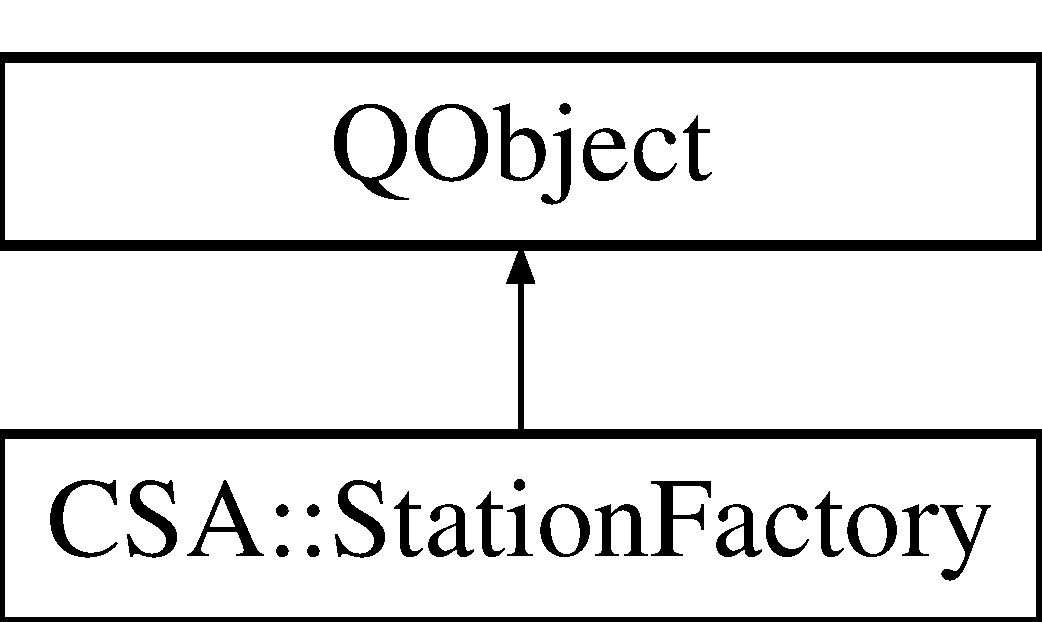
\includegraphics[height=2.000000cm]{classCSA_1_1StationFactory}
\end{center}
\end{figure}
\subsection*{Public Member Functions}
\begin{DoxyCompactItemize}
\item 
\mbox{\hyperlink{classCSA_1_1Station}{Station}} $\ast$ \mbox{\hyperlink{classCSA_1_1StationFactory_ac2abd919e955f56a2c7a2cdba6198160}{get\+Station\+By\+U\+RI}} (const Q\+Url \&uri)
\end{DoxyCompactItemize}
\subsection*{Static Public Member Functions}
\begin{DoxyCompactItemize}
\item 
static \mbox{\hyperlink{classCSA_1_1StationFactory}{Station\+Factory}} $\ast$ \mbox{\hyperlink{classCSA_1_1StationFactory_a445c2886c5ee20b1d86f0d5ed132a53f}{get\+Instance}} (Q\+Object $\ast$parent=nullptr)
\end{DoxyCompactItemize}
\subsection*{Private Member Functions}
\begin{DoxyCompactItemize}
\item 
bool \mbox{\hyperlink{classCSA_1_1StationFactory_a35a69c0ff6abaefbec286ddb775aa41f}{init\+Database}} ()
\item 
bool \mbox{\hyperlink{classCSA_1_1StationFactory_a955892172d726e701332bdd51b4d8c53}{insert\+Station\+With\+Facilities\+Into\+Database}} (const Q\+String\+List \&station, const Q\+String\+List \&facilities)
\item 
bool \mbox{\hyperlink{classCSA_1_1StationFactory_a3edfb2b4e1067ba6d85799784f3df68f}{insert\+Station\+Without\+Facilities\+Into\+Database}} (const Q\+String\+List \&station)
\item 
bool \mbox{\hyperlink{classCSA_1_1StationFactory_a0b7c8552c6e1f389b483daf7ee76d2b3}{insert\+Stop\+Into\+Database}} (const Q\+String\+List \&stop)
\item 
\mbox{\hyperlink{classDatabase_1_1Manager}{Database\+::\+Manager}} $\ast$ \mbox{\hyperlink{classCSA_1_1StationFactory_a402c022930515de30ed15233647b8b72}{db}} () const
\item 
void \mbox{\hyperlink{classCSA_1_1StationFactory_a9f55492093df763b743500a9243c242b}{set\+Db}} (\mbox{\hyperlink{classDatabase_1_1Manager}{Database\+::\+Manager}} $\ast$\mbox{\hyperlink{classCSA_1_1StationFactory_a402c022930515de30ed15233647b8b72}{db}})
\item 
\mbox{\hyperlink{classCSA_1_1StationFactory_ae24ebd450d0a02bc0d431c5fb91f0aa5}{Station\+Factory}} (Q\+Object $\ast$parent)
\end{DoxyCompactItemize}
\subsection*{Private Attributes}
\begin{DoxyCompactItemize}
\item 
\mbox{\hyperlink{classDatabase_1_1Manager}{Database\+::\+Manager}} $\ast$ \mbox{\hyperlink{classCSA_1_1StationFactory_a62dfd390a1c9430d131e0dc72106603c}{m\+\_\+db}}
\end{DoxyCompactItemize}
\subsection*{Static Private Attributes}
\begin{DoxyCompactItemize}
\item 
static \mbox{\hyperlink{classCSA_1_1StationFactory}{C\+S\+A\+::\+Station\+Factory}} $\ast$ \mbox{\hyperlink{classCSA_1_1StationFactory_a23e50080f272055c906807d809334b1b}{m\+\_\+instance}} = nullptr
\end{DoxyCompactItemize}


\subsection{Constructor \& Destructor Documentation}
\mbox{\Hypertarget{classCSA_1_1StationFactory_ae24ebd450d0a02bc0d431c5fb91f0aa5}\label{classCSA_1_1StationFactory_ae24ebd450d0a02bc0d431c5fb91f0aa5}} 
\index{C\+S\+A\+::\+Station\+Factory@{C\+S\+A\+::\+Station\+Factory}!Station\+Factory@{Station\+Factory}}
\index{Station\+Factory@{Station\+Factory}!C\+S\+A\+::\+Station\+Factory@{C\+S\+A\+::\+Station\+Factory}}
\subsubsection{\texorpdfstring{Station\+Factory()}{StationFactory()}}
{\footnotesize\ttfamily C\+S\+A\+::\+Station\+Factory\+::\+Station\+Factory (\begin{DoxyParamCaption}\item[{Q\+Object $\ast$}]{parent }\end{DoxyParamCaption})\hspace{0.3cm}{\ttfamily [explicit]}, {\ttfamily [private]}}



\subsection{Member Function Documentation}
\mbox{\Hypertarget{classCSA_1_1StationFactory_a402c022930515de30ed15233647b8b72}\label{classCSA_1_1StationFactory_a402c022930515de30ed15233647b8b72}} 
\index{C\+S\+A\+::\+Station\+Factory@{C\+S\+A\+::\+Station\+Factory}!db@{db}}
\index{db@{db}!C\+S\+A\+::\+Station\+Factory@{C\+S\+A\+::\+Station\+Factory}}
\subsubsection{\texorpdfstring{db()}{db()}}
{\footnotesize\ttfamily \mbox{\hyperlink{classDatabase_1_1Manager}{Database\+::\+Manager}} $\ast$ C\+S\+A\+::\+Station\+Factory\+::db (\begin{DoxyParamCaption}{ }\end{DoxyParamCaption}) const\hspace{0.3cm}{\ttfamily [private]}}

\mbox{\Hypertarget{classCSA_1_1StationFactory_a445c2886c5ee20b1d86f0d5ed132a53f}\label{classCSA_1_1StationFactory_a445c2886c5ee20b1d86f0d5ed132a53f}} 
\index{C\+S\+A\+::\+Station\+Factory@{C\+S\+A\+::\+Station\+Factory}!get\+Instance@{get\+Instance}}
\index{get\+Instance@{get\+Instance}!C\+S\+A\+::\+Station\+Factory@{C\+S\+A\+::\+Station\+Factory}}
\subsubsection{\texorpdfstring{get\+Instance()}{getInstance()}}
{\footnotesize\ttfamily \mbox{\hyperlink{classCSA_1_1StationFactory}{C\+S\+A\+::\+Station\+Factory}} $\ast$ C\+S\+A\+::\+Station\+Factory\+::get\+Instance (\begin{DoxyParamCaption}\item[{Q\+Object $\ast$}]{parent = {\ttfamily nullptr} }\end{DoxyParamCaption})\hspace{0.3cm}{\ttfamily [static]}}

\mbox{\Hypertarget{classCSA_1_1StationFactory_ac2abd919e955f56a2c7a2cdba6198160}\label{classCSA_1_1StationFactory_ac2abd919e955f56a2c7a2cdba6198160}} 
\index{C\+S\+A\+::\+Station\+Factory@{C\+S\+A\+::\+Station\+Factory}!get\+Station\+By\+U\+RI@{get\+Station\+By\+U\+RI}}
\index{get\+Station\+By\+U\+RI@{get\+Station\+By\+U\+RI}!C\+S\+A\+::\+Station\+Factory@{C\+S\+A\+::\+Station\+Factory}}
\subsubsection{\texorpdfstring{get\+Station\+By\+U\+R\+I()}{getStationByURI()}}
{\footnotesize\ttfamily \mbox{\hyperlink{classCSA_1_1Station}{C\+S\+A\+::\+Station}} $\ast$ C\+S\+A\+::\+Station\+Factory\+::get\+Station\+By\+U\+RI (\begin{DoxyParamCaption}\item[{const Q\+Url \&}]{uri }\end{DoxyParamCaption})}

\mbox{\Hypertarget{classCSA_1_1StationFactory_a35a69c0ff6abaefbec286ddb775aa41f}\label{classCSA_1_1StationFactory_a35a69c0ff6abaefbec286ddb775aa41f}} 
\index{C\+S\+A\+::\+Station\+Factory@{C\+S\+A\+::\+Station\+Factory}!init\+Database@{init\+Database}}
\index{init\+Database@{init\+Database}!C\+S\+A\+::\+Station\+Factory@{C\+S\+A\+::\+Station\+Factory}}
\subsubsection{\texorpdfstring{init\+Database()}{initDatabase()}}
{\footnotesize\ttfamily bool C\+S\+A\+::\+Station\+Factory\+::init\+Database (\begin{DoxyParamCaption}{ }\end{DoxyParamCaption})\hspace{0.3cm}{\ttfamily [private]}}

\mbox{\Hypertarget{classCSA_1_1StationFactory_a955892172d726e701332bdd51b4d8c53}\label{classCSA_1_1StationFactory_a955892172d726e701332bdd51b4d8c53}} 
\index{C\+S\+A\+::\+Station\+Factory@{C\+S\+A\+::\+Station\+Factory}!insert\+Station\+With\+Facilities\+Into\+Database@{insert\+Station\+With\+Facilities\+Into\+Database}}
\index{insert\+Station\+With\+Facilities\+Into\+Database@{insert\+Station\+With\+Facilities\+Into\+Database}!C\+S\+A\+::\+Station\+Factory@{C\+S\+A\+::\+Station\+Factory}}
\subsubsection{\texorpdfstring{insert\+Station\+With\+Facilities\+Into\+Database()}{insertStationWithFacilitiesIntoDatabase()}}
{\footnotesize\ttfamily bool C\+S\+A\+::\+Station\+Factory\+::insert\+Station\+With\+Facilities\+Into\+Database (\begin{DoxyParamCaption}\item[{const Q\+String\+List \&}]{station,  }\item[{const Q\+String\+List \&}]{facilities }\end{DoxyParamCaption})\hspace{0.3cm}{\ttfamily [private]}}

\mbox{\Hypertarget{classCSA_1_1StationFactory_a3edfb2b4e1067ba6d85799784f3df68f}\label{classCSA_1_1StationFactory_a3edfb2b4e1067ba6d85799784f3df68f}} 
\index{C\+S\+A\+::\+Station\+Factory@{C\+S\+A\+::\+Station\+Factory}!insert\+Station\+Without\+Facilities\+Into\+Database@{insert\+Station\+Without\+Facilities\+Into\+Database}}
\index{insert\+Station\+Without\+Facilities\+Into\+Database@{insert\+Station\+Without\+Facilities\+Into\+Database}!C\+S\+A\+::\+Station\+Factory@{C\+S\+A\+::\+Station\+Factory}}
\subsubsection{\texorpdfstring{insert\+Station\+Without\+Facilities\+Into\+Database()}{insertStationWithoutFacilitiesIntoDatabase()}}
{\footnotesize\ttfamily bool C\+S\+A\+::\+Station\+Factory\+::insert\+Station\+Without\+Facilities\+Into\+Database (\begin{DoxyParamCaption}\item[{const Q\+String\+List \&}]{station }\end{DoxyParamCaption})\hspace{0.3cm}{\ttfamily [private]}}

\mbox{\Hypertarget{classCSA_1_1StationFactory_a0b7c8552c6e1f389b483daf7ee76d2b3}\label{classCSA_1_1StationFactory_a0b7c8552c6e1f389b483daf7ee76d2b3}} 
\index{C\+S\+A\+::\+Station\+Factory@{C\+S\+A\+::\+Station\+Factory}!insert\+Stop\+Into\+Database@{insert\+Stop\+Into\+Database}}
\index{insert\+Stop\+Into\+Database@{insert\+Stop\+Into\+Database}!C\+S\+A\+::\+Station\+Factory@{C\+S\+A\+::\+Station\+Factory}}
\subsubsection{\texorpdfstring{insert\+Stop\+Into\+Database()}{insertStopIntoDatabase()}}
{\footnotesize\ttfamily bool C\+S\+A\+::\+Station\+Factory\+::insert\+Stop\+Into\+Database (\begin{DoxyParamCaption}\item[{const Q\+String\+List \&}]{stop }\end{DoxyParamCaption})\hspace{0.3cm}{\ttfamily [private]}}

\mbox{\Hypertarget{classCSA_1_1StationFactory_a9f55492093df763b743500a9243c242b}\label{classCSA_1_1StationFactory_a9f55492093df763b743500a9243c242b}} 
\index{C\+S\+A\+::\+Station\+Factory@{C\+S\+A\+::\+Station\+Factory}!set\+Db@{set\+Db}}
\index{set\+Db@{set\+Db}!C\+S\+A\+::\+Station\+Factory@{C\+S\+A\+::\+Station\+Factory}}
\subsubsection{\texorpdfstring{set\+Db()}{setDb()}}
{\footnotesize\ttfamily void C\+S\+A\+::\+Station\+Factory\+::set\+Db (\begin{DoxyParamCaption}\item[{\mbox{\hyperlink{classDatabase_1_1Manager}{Database\+::\+Manager}} $\ast$}]{db }\end{DoxyParamCaption})\hspace{0.3cm}{\ttfamily [private]}}



\subsection{Member Data Documentation}
\mbox{\Hypertarget{classCSA_1_1StationFactory_a62dfd390a1c9430d131e0dc72106603c}\label{classCSA_1_1StationFactory_a62dfd390a1c9430d131e0dc72106603c}} 
\index{C\+S\+A\+::\+Station\+Factory@{C\+S\+A\+::\+Station\+Factory}!m\+\_\+db@{m\+\_\+db}}
\index{m\+\_\+db@{m\+\_\+db}!C\+S\+A\+::\+Station\+Factory@{C\+S\+A\+::\+Station\+Factory}}
\subsubsection{\texorpdfstring{m\+\_\+db}{m\_db}}
{\footnotesize\ttfamily \mbox{\hyperlink{classDatabase_1_1Manager}{Database\+::\+Manager}}$\ast$ C\+S\+A\+::\+Station\+Factory\+::m\+\_\+db\hspace{0.3cm}{\ttfamily [private]}}

\mbox{\Hypertarget{classCSA_1_1StationFactory_a23e50080f272055c906807d809334b1b}\label{classCSA_1_1StationFactory_a23e50080f272055c906807d809334b1b}} 
\index{C\+S\+A\+::\+Station\+Factory@{C\+S\+A\+::\+Station\+Factory}!m\+\_\+instance@{m\+\_\+instance}}
\index{m\+\_\+instance@{m\+\_\+instance}!C\+S\+A\+::\+Station\+Factory@{C\+S\+A\+::\+Station\+Factory}}
\subsubsection{\texorpdfstring{m\+\_\+instance}{m\_instance}}
{\footnotesize\ttfamily \mbox{\hyperlink{classCSA_1_1StationFactory}{C\+S\+A\+::\+Station\+Factory}} $\ast$ C\+S\+A\+::\+Station\+Factory\+::m\+\_\+instance = nullptr\hspace{0.3cm}{\ttfamily [static]}, {\ttfamily [private]}}



The documentation for this class was generated from the following files\+:\begin{DoxyCompactItemize}
\item 
src/linkedconnections/csa/\mbox{\hyperlink{csastationfactory_8h}{csastationfactory.\+h}}\item 
src/linkedconnections/csa/\mbox{\hyperlink{csastationfactory_8cpp}{csastationfactory.\+cpp}}\end{DoxyCompactItemize}

\hypertarget{classCSA_1_1StationStopProfile}{}\section{C\+SA\+:\+:Station\+Stop\+Profile Class Reference}
\label{classCSA_1_1StationStopProfile}\index{C\+S\+A\+::\+Station\+Stop\+Profile@{C\+S\+A\+::\+Station\+Stop\+Profile}}


{\ttfamily \#include $<$csastationstopprofile.\+h$>$}

Inheritance diagram for C\+SA\+:\+:Station\+Stop\+Profile\+:\begin{figure}[H]
\begin{center}
\leavevmode
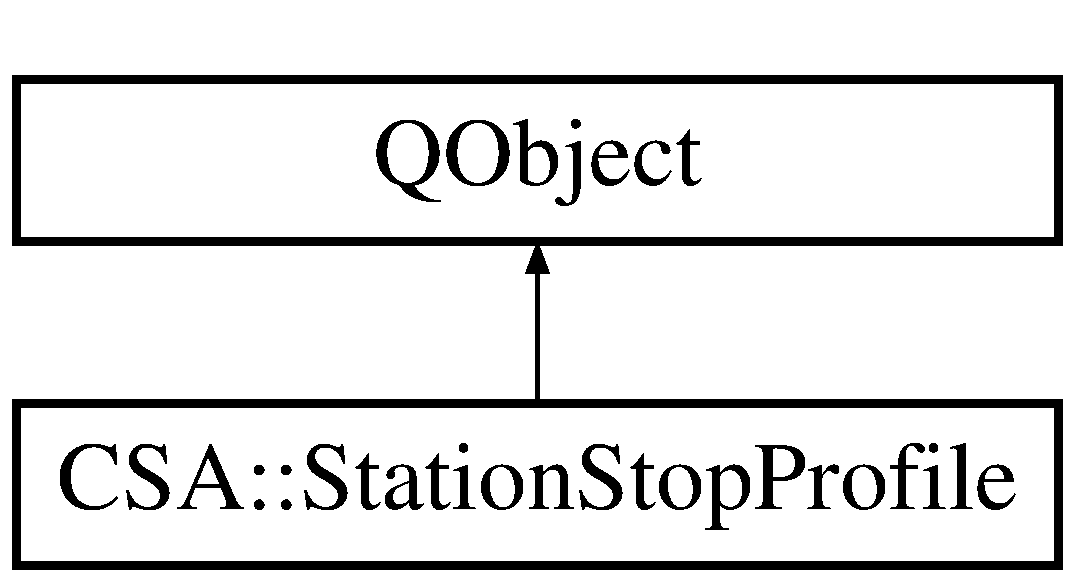
\includegraphics[height=2.000000cm]{classCSA_1_1StationStopProfile}
\end{center}
\end{figure}
\subsection*{Signals}
\begin{DoxyCompactItemize}
\item 
void \mbox{\hyperlink{classCSA_1_1StationStopProfile_a2cd652ab0ec1ab2d2a30ef175c85dc71}{departure\+Time\+Changed}} ()
\item 
void \mbox{\hyperlink{classCSA_1_1StationStopProfile_af4e461e3d6a947fd640c2c871d41f5e9}{arrival\+Time\+Changed}} ()
\item 
void \mbox{\hyperlink{classCSA_1_1StationStopProfile_a45b8bc33cb7ea716b2ed8a6ec8dd4db0}{departure\+Connection\+Changed}} ()
\item 
void \mbox{\hyperlink{classCSA_1_1StationStopProfile_a3f7b89aa6a83653ae32102ccb04175cb}{arrival\+Connection\+Changed}} ()
\item 
void \mbox{\hyperlink{classCSA_1_1StationStopProfile_a7035ce1d247c7feff5b1df96e654110f}{transfers\+Changed}} ()
\end{DoxyCompactItemize}
\subsection*{Public Member Functions}
\begin{DoxyCompactItemize}
\item 
\mbox{\hyperlink{classCSA_1_1StationStopProfile_aaad218564513e0a629a4b1e596c24d7f}{Station\+Stop\+Profile}} (const Q\+Date\+Time \&\mbox{\hyperlink{classCSA_1_1StationStopProfile_afef345e7edf4dbd8effec87ab565d030}{departure\+Time}}, const Q\+Date\+Time \&\mbox{\hyperlink{classCSA_1_1StationStopProfile_a33c9f8331164a7af0884a26ee24940b7}{arrival\+Time}}, \mbox{\hyperlink{classFragments_1_1Fragment}{Fragments\+::\+Fragment}} $\ast$\mbox{\hyperlink{classCSA_1_1StationStopProfile_ac75cf7fddd5db7abd8b788849b78263e}{departure\+Connection}}, \mbox{\hyperlink{classFragments_1_1Fragment}{Fragments\+::\+Fragment}} $\ast$\mbox{\hyperlink{classCSA_1_1StationStopProfile_a6cfce145f35c2263a21a207844470bec}{arrival\+Connection}}, const qint16 \mbox{\hyperlink{classCSA_1_1StationStopProfile_a10a03b9f10dec06eac01f970c77b3ada}{transfers}}, Q\+Object $\ast$parent=nullptr)
\item 
Q\+Date\+Time \mbox{\hyperlink{classCSA_1_1StationStopProfile_afef345e7edf4dbd8effec87ab565d030}{departure\+Time}} () const
\item 
void \mbox{\hyperlink{classCSA_1_1StationStopProfile_a55ed54cba17d902390d2030003177059}{set\+Departure\+Time}} (const Q\+Date\+Time \&\mbox{\hyperlink{classCSA_1_1StationStopProfile_afef345e7edf4dbd8effec87ab565d030}{departure\+Time}})
\item 
Q\+Date\+Time \mbox{\hyperlink{classCSA_1_1StationStopProfile_a33c9f8331164a7af0884a26ee24940b7}{arrival\+Time}} () const
\item 
void \mbox{\hyperlink{classCSA_1_1StationStopProfile_ac6690454adee23fde8d7ff5abd42396d}{set\+Arrival\+Time}} (const Q\+Date\+Time \&\mbox{\hyperlink{classCSA_1_1StationStopProfile_a33c9f8331164a7af0884a26ee24940b7}{arrival\+Time}})
\item 
\mbox{\hyperlink{classFragments_1_1Fragment}{Fragments\+::\+Fragment}} $\ast$ \mbox{\hyperlink{classCSA_1_1StationStopProfile_ac75cf7fddd5db7abd8b788849b78263e}{departure\+Connection}} () const
\item 
void \mbox{\hyperlink{classCSA_1_1StationStopProfile_a2d53816b9df7e028d96591006c56bc30}{set\+Departure\+Connection}} (\mbox{\hyperlink{classFragments_1_1Fragment}{Fragments\+::\+Fragment}} $\ast$\mbox{\hyperlink{classCSA_1_1StationStopProfile_ac75cf7fddd5db7abd8b788849b78263e}{departure\+Connection}})
\item 
\mbox{\hyperlink{classFragments_1_1Fragment}{Fragments\+::\+Fragment}} $\ast$ \mbox{\hyperlink{classCSA_1_1StationStopProfile_a6cfce145f35c2263a21a207844470bec}{arrival\+Connection}} () const
\item 
void \mbox{\hyperlink{classCSA_1_1StationStopProfile_aaf7ff4817f02d371363fd7d9cb3981cc}{set\+Arrival\+Connection}} (\mbox{\hyperlink{classFragments_1_1Fragment}{Fragments\+::\+Fragment}} $\ast$\mbox{\hyperlink{classCSA_1_1StationStopProfile_a6cfce145f35c2263a21a207844470bec}{arrival\+Connection}})
\item 
qint16 \mbox{\hyperlink{classCSA_1_1StationStopProfile_a10a03b9f10dec06eac01f970c77b3ada}{transfers}} () const
\item 
void \mbox{\hyperlink{classCSA_1_1StationStopProfile_a52596359c1750e648a907dffba3c6a42}{set\+Transfers}} (const qint16 \&\mbox{\hyperlink{classCSA_1_1StationStopProfile_a10a03b9f10dec06eac01f970c77b3ada}{transfers}})
\end{DoxyCompactItemize}
\subsection*{Private Attributes}
\begin{DoxyCompactItemize}
\item 
Q\+Date\+Time \mbox{\hyperlink{classCSA_1_1StationStopProfile_ade3eb19735433a7ab6956ac34d023e3b}{m\+\_\+departure\+Time}}
\item 
Q\+Date\+Time \mbox{\hyperlink{classCSA_1_1StationStopProfile_a652144ad18e1d039364301c909d316aa}{m\+\_\+arrival\+Time}}
\item 
\mbox{\hyperlink{classFragments_1_1Fragment}{Fragments\+::\+Fragment}} $\ast$ \mbox{\hyperlink{classCSA_1_1StationStopProfile_a999eea44e28580f8f6783e488c0d028b}{m\+\_\+departure\+Connection}}
\item 
\mbox{\hyperlink{classFragments_1_1Fragment}{Fragments\+::\+Fragment}} $\ast$ \mbox{\hyperlink{classCSA_1_1StationStopProfile_afc632c63a7644b64241af818cf6cf179}{m\+\_\+arrival\+Connection}}
\item 
qint16 \mbox{\hyperlink{classCSA_1_1StationStopProfile_a9616f115681c835b03975aab6bb3dfae}{m\+\_\+transfers}}
\end{DoxyCompactItemize}


\subsection{Constructor \& Destructor Documentation}
\mbox{\Hypertarget{classCSA_1_1StationStopProfile_aaad218564513e0a629a4b1e596c24d7f}\label{classCSA_1_1StationStopProfile_aaad218564513e0a629a4b1e596c24d7f}} 
\index{C\+S\+A\+::\+Station\+Stop\+Profile@{C\+S\+A\+::\+Station\+Stop\+Profile}!Station\+Stop\+Profile@{Station\+Stop\+Profile}}
\index{Station\+Stop\+Profile@{Station\+Stop\+Profile}!C\+S\+A\+::\+Station\+Stop\+Profile@{C\+S\+A\+::\+Station\+Stop\+Profile}}
\subsubsection{\texorpdfstring{Station\+Stop\+Profile()}{StationStopProfile()}}
{\footnotesize\ttfamily C\+S\+A\+::\+Station\+Stop\+Profile\+::\+Station\+Stop\+Profile (\begin{DoxyParamCaption}\item[{const Q\+Date\+Time \&}]{departure\+Time,  }\item[{const Q\+Date\+Time \&}]{arrival\+Time,  }\item[{\mbox{\hyperlink{classFragments_1_1Fragment}{Fragments\+::\+Fragment}} $\ast$}]{departure\+Connection,  }\item[{\mbox{\hyperlink{classFragments_1_1Fragment}{Fragments\+::\+Fragment}} $\ast$}]{arrival\+Connection,  }\item[{const qint16}]{transfers,  }\item[{Q\+Object $\ast$}]{parent = {\ttfamily nullptr} }\end{DoxyParamCaption})\hspace{0.3cm}{\ttfamily [explicit]}}



\subsection{Member Function Documentation}
\mbox{\Hypertarget{classCSA_1_1StationStopProfile_a6cfce145f35c2263a21a207844470bec}\label{classCSA_1_1StationStopProfile_a6cfce145f35c2263a21a207844470bec}} 
\index{C\+S\+A\+::\+Station\+Stop\+Profile@{C\+S\+A\+::\+Station\+Stop\+Profile}!arrival\+Connection@{arrival\+Connection}}
\index{arrival\+Connection@{arrival\+Connection}!C\+S\+A\+::\+Station\+Stop\+Profile@{C\+S\+A\+::\+Station\+Stop\+Profile}}
\subsubsection{\texorpdfstring{arrival\+Connection()}{arrivalConnection()}}
{\footnotesize\ttfamily \mbox{\hyperlink{classFragments_1_1Fragment}{Fragments\+::\+Fragment}} $\ast$ C\+S\+A\+::\+Station\+Stop\+Profile\+::arrival\+Connection (\begin{DoxyParamCaption}{ }\end{DoxyParamCaption}) const}

\mbox{\Hypertarget{classCSA_1_1StationStopProfile_a3f7b89aa6a83653ae32102ccb04175cb}\label{classCSA_1_1StationStopProfile_a3f7b89aa6a83653ae32102ccb04175cb}} 
\index{C\+S\+A\+::\+Station\+Stop\+Profile@{C\+S\+A\+::\+Station\+Stop\+Profile}!arrival\+Connection\+Changed@{arrival\+Connection\+Changed}}
\index{arrival\+Connection\+Changed@{arrival\+Connection\+Changed}!C\+S\+A\+::\+Station\+Stop\+Profile@{C\+S\+A\+::\+Station\+Stop\+Profile}}
\subsubsection{\texorpdfstring{arrival\+Connection\+Changed}{arrivalConnectionChanged}}
{\footnotesize\ttfamily void C\+S\+A\+::\+Station\+Stop\+Profile\+::arrival\+Connection\+Changed (\begin{DoxyParamCaption}{ }\end{DoxyParamCaption})\hspace{0.3cm}{\ttfamily [signal]}}

\mbox{\Hypertarget{classCSA_1_1StationStopProfile_a33c9f8331164a7af0884a26ee24940b7}\label{classCSA_1_1StationStopProfile_a33c9f8331164a7af0884a26ee24940b7}} 
\index{C\+S\+A\+::\+Station\+Stop\+Profile@{C\+S\+A\+::\+Station\+Stop\+Profile}!arrival\+Time@{arrival\+Time}}
\index{arrival\+Time@{arrival\+Time}!C\+S\+A\+::\+Station\+Stop\+Profile@{C\+S\+A\+::\+Station\+Stop\+Profile}}
\subsubsection{\texorpdfstring{arrival\+Time()}{arrivalTime()}}
{\footnotesize\ttfamily Q\+Date\+Time C\+S\+A\+::\+Station\+Stop\+Profile\+::arrival\+Time (\begin{DoxyParamCaption}{ }\end{DoxyParamCaption}) const}

\mbox{\Hypertarget{classCSA_1_1StationStopProfile_af4e461e3d6a947fd640c2c871d41f5e9}\label{classCSA_1_1StationStopProfile_af4e461e3d6a947fd640c2c871d41f5e9}} 
\index{C\+S\+A\+::\+Station\+Stop\+Profile@{C\+S\+A\+::\+Station\+Stop\+Profile}!arrival\+Time\+Changed@{arrival\+Time\+Changed}}
\index{arrival\+Time\+Changed@{arrival\+Time\+Changed}!C\+S\+A\+::\+Station\+Stop\+Profile@{C\+S\+A\+::\+Station\+Stop\+Profile}}
\subsubsection{\texorpdfstring{arrival\+Time\+Changed}{arrivalTimeChanged}}
{\footnotesize\ttfamily void C\+S\+A\+::\+Station\+Stop\+Profile\+::arrival\+Time\+Changed (\begin{DoxyParamCaption}{ }\end{DoxyParamCaption})\hspace{0.3cm}{\ttfamily [signal]}}

\mbox{\Hypertarget{classCSA_1_1StationStopProfile_ac75cf7fddd5db7abd8b788849b78263e}\label{classCSA_1_1StationStopProfile_ac75cf7fddd5db7abd8b788849b78263e}} 
\index{C\+S\+A\+::\+Station\+Stop\+Profile@{C\+S\+A\+::\+Station\+Stop\+Profile}!departure\+Connection@{departure\+Connection}}
\index{departure\+Connection@{departure\+Connection}!C\+S\+A\+::\+Station\+Stop\+Profile@{C\+S\+A\+::\+Station\+Stop\+Profile}}
\subsubsection{\texorpdfstring{departure\+Connection()}{departureConnection()}}
{\footnotesize\ttfamily \mbox{\hyperlink{classFragments_1_1Fragment}{Fragments\+::\+Fragment}} $\ast$ C\+S\+A\+::\+Station\+Stop\+Profile\+::departure\+Connection (\begin{DoxyParamCaption}{ }\end{DoxyParamCaption}) const}

\mbox{\Hypertarget{classCSA_1_1StationStopProfile_a45b8bc33cb7ea716b2ed8a6ec8dd4db0}\label{classCSA_1_1StationStopProfile_a45b8bc33cb7ea716b2ed8a6ec8dd4db0}} 
\index{C\+S\+A\+::\+Station\+Stop\+Profile@{C\+S\+A\+::\+Station\+Stop\+Profile}!departure\+Connection\+Changed@{departure\+Connection\+Changed}}
\index{departure\+Connection\+Changed@{departure\+Connection\+Changed}!C\+S\+A\+::\+Station\+Stop\+Profile@{C\+S\+A\+::\+Station\+Stop\+Profile}}
\subsubsection{\texorpdfstring{departure\+Connection\+Changed}{departureConnectionChanged}}
{\footnotesize\ttfamily void C\+S\+A\+::\+Station\+Stop\+Profile\+::departure\+Connection\+Changed (\begin{DoxyParamCaption}{ }\end{DoxyParamCaption})\hspace{0.3cm}{\ttfamily [signal]}}

\mbox{\Hypertarget{classCSA_1_1StationStopProfile_afef345e7edf4dbd8effec87ab565d030}\label{classCSA_1_1StationStopProfile_afef345e7edf4dbd8effec87ab565d030}} 
\index{C\+S\+A\+::\+Station\+Stop\+Profile@{C\+S\+A\+::\+Station\+Stop\+Profile}!departure\+Time@{departure\+Time}}
\index{departure\+Time@{departure\+Time}!C\+S\+A\+::\+Station\+Stop\+Profile@{C\+S\+A\+::\+Station\+Stop\+Profile}}
\subsubsection{\texorpdfstring{departure\+Time()}{departureTime()}}
{\footnotesize\ttfamily Q\+Date\+Time C\+S\+A\+::\+Station\+Stop\+Profile\+::departure\+Time (\begin{DoxyParamCaption}{ }\end{DoxyParamCaption}) const}

\mbox{\Hypertarget{classCSA_1_1StationStopProfile_a2cd652ab0ec1ab2d2a30ef175c85dc71}\label{classCSA_1_1StationStopProfile_a2cd652ab0ec1ab2d2a30ef175c85dc71}} 
\index{C\+S\+A\+::\+Station\+Stop\+Profile@{C\+S\+A\+::\+Station\+Stop\+Profile}!departure\+Time\+Changed@{departure\+Time\+Changed}}
\index{departure\+Time\+Changed@{departure\+Time\+Changed}!C\+S\+A\+::\+Station\+Stop\+Profile@{C\+S\+A\+::\+Station\+Stop\+Profile}}
\subsubsection{\texorpdfstring{departure\+Time\+Changed}{departureTimeChanged}}
{\footnotesize\ttfamily void C\+S\+A\+::\+Station\+Stop\+Profile\+::departure\+Time\+Changed (\begin{DoxyParamCaption}{ }\end{DoxyParamCaption})\hspace{0.3cm}{\ttfamily [signal]}}

\mbox{\Hypertarget{classCSA_1_1StationStopProfile_aaf7ff4817f02d371363fd7d9cb3981cc}\label{classCSA_1_1StationStopProfile_aaf7ff4817f02d371363fd7d9cb3981cc}} 
\index{C\+S\+A\+::\+Station\+Stop\+Profile@{C\+S\+A\+::\+Station\+Stop\+Profile}!set\+Arrival\+Connection@{set\+Arrival\+Connection}}
\index{set\+Arrival\+Connection@{set\+Arrival\+Connection}!C\+S\+A\+::\+Station\+Stop\+Profile@{C\+S\+A\+::\+Station\+Stop\+Profile}}
\subsubsection{\texorpdfstring{set\+Arrival\+Connection()}{setArrivalConnection()}}
{\footnotesize\ttfamily void C\+S\+A\+::\+Station\+Stop\+Profile\+::set\+Arrival\+Connection (\begin{DoxyParamCaption}\item[{\mbox{\hyperlink{classFragments_1_1Fragment}{Fragments\+::\+Fragment}} $\ast$}]{arrival\+Connection }\end{DoxyParamCaption})}

\mbox{\Hypertarget{classCSA_1_1StationStopProfile_ac6690454adee23fde8d7ff5abd42396d}\label{classCSA_1_1StationStopProfile_ac6690454adee23fde8d7ff5abd42396d}} 
\index{C\+S\+A\+::\+Station\+Stop\+Profile@{C\+S\+A\+::\+Station\+Stop\+Profile}!set\+Arrival\+Time@{set\+Arrival\+Time}}
\index{set\+Arrival\+Time@{set\+Arrival\+Time}!C\+S\+A\+::\+Station\+Stop\+Profile@{C\+S\+A\+::\+Station\+Stop\+Profile}}
\subsubsection{\texorpdfstring{set\+Arrival\+Time()}{setArrivalTime()}}
{\footnotesize\ttfamily void C\+S\+A\+::\+Station\+Stop\+Profile\+::set\+Arrival\+Time (\begin{DoxyParamCaption}\item[{const Q\+Date\+Time \&}]{arrival\+Time }\end{DoxyParamCaption})}

\mbox{\Hypertarget{classCSA_1_1StationStopProfile_a2d53816b9df7e028d96591006c56bc30}\label{classCSA_1_1StationStopProfile_a2d53816b9df7e028d96591006c56bc30}} 
\index{C\+S\+A\+::\+Station\+Stop\+Profile@{C\+S\+A\+::\+Station\+Stop\+Profile}!set\+Departure\+Connection@{set\+Departure\+Connection}}
\index{set\+Departure\+Connection@{set\+Departure\+Connection}!C\+S\+A\+::\+Station\+Stop\+Profile@{C\+S\+A\+::\+Station\+Stop\+Profile}}
\subsubsection{\texorpdfstring{set\+Departure\+Connection()}{setDepartureConnection()}}
{\footnotesize\ttfamily void C\+S\+A\+::\+Station\+Stop\+Profile\+::set\+Departure\+Connection (\begin{DoxyParamCaption}\item[{\mbox{\hyperlink{classFragments_1_1Fragment}{Fragments\+::\+Fragment}} $\ast$}]{departure\+Connection }\end{DoxyParamCaption})}

\mbox{\Hypertarget{classCSA_1_1StationStopProfile_a55ed54cba17d902390d2030003177059}\label{classCSA_1_1StationStopProfile_a55ed54cba17d902390d2030003177059}} 
\index{C\+S\+A\+::\+Station\+Stop\+Profile@{C\+S\+A\+::\+Station\+Stop\+Profile}!set\+Departure\+Time@{set\+Departure\+Time}}
\index{set\+Departure\+Time@{set\+Departure\+Time}!C\+S\+A\+::\+Station\+Stop\+Profile@{C\+S\+A\+::\+Station\+Stop\+Profile}}
\subsubsection{\texorpdfstring{set\+Departure\+Time()}{setDepartureTime()}}
{\footnotesize\ttfamily void C\+S\+A\+::\+Station\+Stop\+Profile\+::set\+Departure\+Time (\begin{DoxyParamCaption}\item[{const Q\+Date\+Time \&}]{departure\+Time }\end{DoxyParamCaption})}

\mbox{\Hypertarget{classCSA_1_1StationStopProfile_a52596359c1750e648a907dffba3c6a42}\label{classCSA_1_1StationStopProfile_a52596359c1750e648a907dffba3c6a42}} 
\index{C\+S\+A\+::\+Station\+Stop\+Profile@{C\+S\+A\+::\+Station\+Stop\+Profile}!set\+Transfers@{set\+Transfers}}
\index{set\+Transfers@{set\+Transfers}!C\+S\+A\+::\+Station\+Stop\+Profile@{C\+S\+A\+::\+Station\+Stop\+Profile}}
\subsubsection{\texorpdfstring{set\+Transfers()}{setTransfers()}}
{\footnotesize\ttfamily void C\+S\+A\+::\+Station\+Stop\+Profile\+::set\+Transfers (\begin{DoxyParamCaption}\item[{const qint16 \&}]{transfers }\end{DoxyParamCaption})}

\mbox{\Hypertarget{classCSA_1_1StationStopProfile_a10a03b9f10dec06eac01f970c77b3ada}\label{classCSA_1_1StationStopProfile_a10a03b9f10dec06eac01f970c77b3ada}} 
\index{C\+S\+A\+::\+Station\+Stop\+Profile@{C\+S\+A\+::\+Station\+Stop\+Profile}!transfers@{transfers}}
\index{transfers@{transfers}!C\+S\+A\+::\+Station\+Stop\+Profile@{C\+S\+A\+::\+Station\+Stop\+Profile}}
\subsubsection{\texorpdfstring{transfers()}{transfers()}}
{\footnotesize\ttfamily qint16 C\+S\+A\+::\+Station\+Stop\+Profile\+::transfers (\begin{DoxyParamCaption}{ }\end{DoxyParamCaption}) const}

\mbox{\Hypertarget{classCSA_1_1StationStopProfile_a7035ce1d247c7feff5b1df96e654110f}\label{classCSA_1_1StationStopProfile_a7035ce1d247c7feff5b1df96e654110f}} 
\index{C\+S\+A\+::\+Station\+Stop\+Profile@{C\+S\+A\+::\+Station\+Stop\+Profile}!transfers\+Changed@{transfers\+Changed}}
\index{transfers\+Changed@{transfers\+Changed}!C\+S\+A\+::\+Station\+Stop\+Profile@{C\+S\+A\+::\+Station\+Stop\+Profile}}
\subsubsection{\texorpdfstring{transfers\+Changed}{transfersChanged}}
{\footnotesize\ttfamily void C\+S\+A\+::\+Station\+Stop\+Profile\+::transfers\+Changed (\begin{DoxyParamCaption}{ }\end{DoxyParamCaption})\hspace{0.3cm}{\ttfamily [signal]}}



\subsection{Member Data Documentation}
\mbox{\Hypertarget{classCSA_1_1StationStopProfile_afc632c63a7644b64241af818cf6cf179}\label{classCSA_1_1StationStopProfile_afc632c63a7644b64241af818cf6cf179}} 
\index{C\+S\+A\+::\+Station\+Stop\+Profile@{C\+S\+A\+::\+Station\+Stop\+Profile}!m\+\_\+arrival\+Connection@{m\+\_\+arrival\+Connection}}
\index{m\+\_\+arrival\+Connection@{m\+\_\+arrival\+Connection}!C\+S\+A\+::\+Station\+Stop\+Profile@{C\+S\+A\+::\+Station\+Stop\+Profile}}
\subsubsection{\texorpdfstring{m\+\_\+arrival\+Connection}{m\_arrivalConnection}}
{\footnotesize\ttfamily \mbox{\hyperlink{classFragments_1_1Fragment}{Fragments\+::\+Fragment}}$\ast$ C\+S\+A\+::\+Station\+Stop\+Profile\+::m\+\_\+arrival\+Connection\hspace{0.3cm}{\ttfamily [private]}}

\mbox{\Hypertarget{classCSA_1_1StationStopProfile_a652144ad18e1d039364301c909d316aa}\label{classCSA_1_1StationStopProfile_a652144ad18e1d039364301c909d316aa}} 
\index{C\+S\+A\+::\+Station\+Stop\+Profile@{C\+S\+A\+::\+Station\+Stop\+Profile}!m\+\_\+arrival\+Time@{m\+\_\+arrival\+Time}}
\index{m\+\_\+arrival\+Time@{m\+\_\+arrival\+Time}!C\+S\+A\+::\+Station\+Stop\+Profile@{C\+S\+A\+::\+Station\+Stop\+Profile}}
\subsubsection{\texorpdfstring{m\+\_\+arrival\+Time}{m\_arrivalTime}}
{\footnotesize\ttfamily Q\+Date\+Time C\+S\+A\+::\+Station\+Stop\+Profile\+::m\+\_\+arrival\+Time\hspace{0.3cm}{\ttfamily [private]}}

\mbox{\Hypertarget{classCSA_1_1StationStopProfile_a999eea44e28580f8f6783e488c0d028b}\label{classCSA_1_1StationStopProfile_a999eea44e28580f8f6783e488c0d028b}} 
\index{C\+S\+A\+::\+Station\+Stop\+Profile@{C\+S\+A\+::\+Station\+Stop\+Profile}!m\+\_\+departure\+Connection@{m\+\_\+departure\+Connection}}
\index{m\+\_\+departure\+Connection@{m\+\_\+departure\+Connection}!C\+S\+A\+::\+Station\+Stop\+Profile@{C\+S\+A\+::\+Station\+Stop\+Profile}}
\subsubsection{\texorpdfstring{m\+\_\+departure\+Connection}{m\_departureConnection}}
{\footnotesize\ttfamily \mbox{\hyperlink{classFragments_1_1Fragment}{Fragments\+::\+Fragment}}$\ast$ C\+S\+A\+::\+Station\+Stop\+Profile\+::m\+\_\+departure\+Connection\hspace{0.3cm}{\ttfamily [private]}}

\mbox{\Hypertarget{classCSA_1_1StationStopProfile_ade3eb19735433a7ab6956ac34d023e3b}\label{classCSA_1_1StationStopProfile_ade3eb19735433a7ab6956ac34d023e3b}} 
\index{C\+S\+A\+::\+Station\+Stop\+Profile@{C\+S\+A\+::\+Station\+Stop\+Profile}!m\+\_\+departure\+Time@{m\+\_\+departure\+Time}}
\index{m\+\_\+departure\+Time@{m\+\_\+departure\+Time}!C\+S\+A\+::\+Station\+Stop\+Profile@{C\+S\+A\+::\+Station\+Stop\+Profile}}
\subsubsection{\texorpdfstring{m\+\_\+departure\+Time}{m\_departureTime}}
{\footnotesize\ttfamily Q\+Date\+Time C\+S\+A\+::\+Station\+Stop\+Profile\+::m\+\_\+departure\+Time\hspace{0.3cm}{\ttfamily [private]}}

\mbox{\Hypertarget{classCSA_1_1StationStopProfile_a9616f115681c835b03975aab6bb3dfae}\label{classCSA_1_1StationStopProfile_a9616f115681c835b03975aab6bb3dfae}} 
\index{C\+S\+A\+::\+Station\+Stop\+Profile@{C\+S\+A\+::\+Station\+Stop\+Profile}!m\+\_\+transfers@{m\+\_\+transfers}}
\index{m\+\_\+transfers@{m\+\_\+transfers}!C\+S\+A\+::\+Station\+Stop\+Profile@{C\+S\+A\+::\+Station\+Stop\+Profile}}
\subsubsection{\texorpdfstring{m\+\_\+transfers}{m\_transfers}}
{\footnotesize\ttfamily qint16 C\+S\+A\+::\+Station\+Stop\+Profile\+::m\+\_\+transfers\hspace{0.3cm}{\ttfamily [private]}}



The documentation for this class was generated from the following files\+:\begin{DoxyCompactItemize}
\item 
src/linkedconnections/csa/\mbox{\hyperlink{csastationstopprofile_8h}{csastationstopprofile.\+h}}\item 
src/linkedconnections/csa/\mbox{\hyperlink{csastationstopprofile_8cpp}{csastationstopprofile.\+cpp}}\end{DoxyCompactItemize}

\hypertarget{classCSA_1_1TrainProfile}{}\section{C\+SA\+:\+:Train\+Profile Class Reference}
\label{classCSA_1_1TrainProfile}\index{C\+S\+A\+::\+Train\+Profile@{C\+S\+A\+::\+Train\+Profile}}


{\ttfamily \#include $<$csatrainprofile.\+h$>$}

Inheritance diagram for C\+SA\+:\+:Train\+Profile\+:\begin{figure}[H]
\begin{center}
\leavevmode
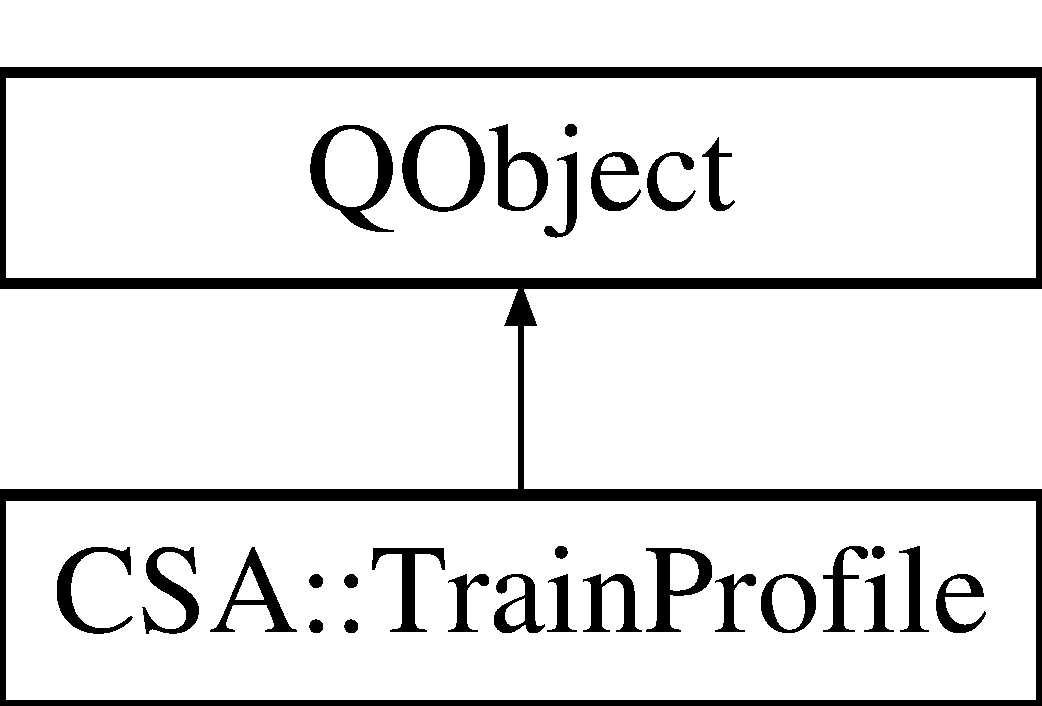
\includegraphics[height=2.000000cm]{classCSA_1_1TrainProfile}
\end{center}
\end{figure}
\subsection*{Signals}
\begin{DoxyCompactItemize}
\item 
void \mbox{\hyperlink{classCSA_1_1TrainProfile_a0acb40ad012f423a6312616ee7598265}{arrival\+Time\+Changed}} ()
\item 
void \mbox{\hyperlink{classCSA_1_1TrainProfile_ab5fdfaa36c183f15300d4c61286440e9}{arrival\+Connection\+Changed}} ()
\item 
void \mbox{\hyperlink{classCSA_1_1TrainProfile_aec2a0ddcf55785288eede5b45013a344}{transfers\+Changed}} ()
\end{DoxyCompactItemize}
\subsection*{Public Member Functions}
\begin{DoxyCompactItemize}
\item 
\mbox{\hyperlink{classCSA_1_1TrainProfile_ac939a2e59e0b5ef149225af1b1c4b0f9}{Train\+Profile}} (const Q\+Date\+Time \&\mbox{\hyperlink{classCSA_1_1TrainProfile_a3892c881f8a4ce8fd7a9366011ccc4b1}{arrival\+Time}}, \mbox{\hyperlink{classFragments_1_1Fragment}{Fragments\+::\+Fragment}} $\ast$\mbox{\hyperlink{classCSA_1_1TrainProfile_a2a7907625e22799ad36acc22ef23c7ae}{arrival\+Connection}}, const qint16 \mbox{\hyperlink{classCSA_1_1TrainProfile_a9e0520e5ebf6ad00c0462a428300caad}{transfers}}, Q\+Object $\ast$parent=nullptr)
\item 
Q\+Date\+Time \mbox{\hyperlink{classCSA_1_1TrainProfile_a3892c881f8a4ce8fd7a9366011ccc4b1}{arrival\+Time}} () const
\item 
void \mbox{\hyperlink{classCSA_1_1TrainProfile_ae2701384d61bd3ed4dbc7b3b1beeb02e}{set\+Arrival\+Time}} (const Q\+Date\+Time \&\mbox{\hyperlink{classCSA_1_1TrainProfile_a3892c881f8a4ce8fd7a9366011ccc4b1}{arrival\+Time}})
\item 
\mbox{\hyperlink{classFragments_1_1Fragment}{Fragments\+::\+Fragment}} $\ast$ \mbox{\hyperlink{classCSA_1_1TrainProfile_a2a7907625e22799ad36acc22ef23c7ae}{arrival\+Connection}} () const
\item 
void \mbox{\hyperlink{classCSA_1_1TrainProfile_a18c7b5ea923eededaa6965d0e89b1770}{set\+Arrival\+Connection}} (\mbox{\hyperlink{classFragments_1_1Fragment}{Fragments\+::\+Fragment}} $\ast$\mbox{\hyperlink{classCSA_1_1TrainProfile_a2a7907625e22799ad36acc22ef23c7ae}{arrival\+Connection}})
\item 
qint16 \mbox{\hyperlink{classCSA_1_1TrainProfile_a9e0520e5ebf6ad00c0462a428300caad}{transfers}} () const
\item 
void \mbox{\hyperlink{classCSA_1_1TrainProfile_a5507b82c5ef60c32682e662dc6a113f2}{set\+Transfers}} (const qint16 \&\mbox{\hyperlink{classCSA_1_1TrainProfile_a9e0520e5ebf6ad00c0462a428300caad}{transfers}})
\end{DoxyCompactItemize}
\subsection*{Private Attributes}
\begin{DoxyCompactItemize}
\item 
Q\+Date\+Time \mbox{\hyperlink{classCSA_1_1TrainProfile_adba3b60fe32bdd008973662cd4c0a722}{m\+\_\+arrival\+Time}}
\item 
\mbox{\hyperlink{classFragments_1_1Fragment}{Fragments\+::\+Fragment}} $\ast$ \mbox{\hyperlink{classCSA_1_1TrainProfile_ae0987377d3eb8bdedf29c866a8d2a1e3}{m\+\_\+arrival\+Connection}}
\item 
qint16 \mbox{\hyperlink{classCSA_1_1TrainProfile_af0a6f25b6a87259edfe8a4024176d2fd}{m\+\_\+transfers}}
\end{DoxyCompactItemize}


\subsection{Constructor \& Destructor Documentation}
\mbox{\Hypertarget{classCSA_1_1TrainProfile_ac939a2e59e0b5ef149225af1b1c4b0f9}\label{classCSA_1_1TrainProfile_ac939a2e59e0b5ef149225af1b1c4b0f9}} 
\index{C\+S\+A\+::\+Train\+Profile@{C\+S\+A\+::\+Train\+Profile}!Train\+Profile@{Train\+Profile}}
\index{Train\+Profile@{Train\+Profile}!C\+S\+A\+::\+Train\+Profile@{C\+S\+A\+::\+Train\+Profile}}
\subsubsection{\texorpdfstring{Train\+Profile()}{TrainProfile()}}
{\footnotesize\ttfamily C\+S\+A\+::\+Train\+Profile\+::\+Train\+Profile (\begin{DoxyParamCaption}\item[{const Q\+Date\+Time \&}]{arrival\+Time,  }\item[{\mbox{\hyperlink{classFragments_1_1Fragment}{Fragments\+::\+Fragment}} $\ast$}]{arrival\+Connection,  }\item[{const qint16}]{transfers,  }\item[{Q\+Object $\ast$}]{parent = {\ttfamily nullptr} }\end{DoxyParamCaption})\hspace{0.3cm}{\ttfamily [explicit]}}



\subsection{Member Function Documentation}
\mbox{\Hypertarget{classCSA_1_1TrainProfile_a2a7907625e22799ad36acc22ef23c7ae}\label{classCSA_1_1TrainProfile_a2a7907625e22799ad36acc22ef23c7ae}} 
\index{C\+S\+A\+::\+Train\+Profile@{C\+S\+A\+::\+Train\+Profile}!arrival\+Connection@{arrival\+Connection}}
\index{arrival\+Connection@{arrival\+Connection}!C\+S\+A\+::\+Train\+Profile@{C\+S\+A\+::\+Train\+Profile}}
\subsubsection{\texorpdfstring{arrival\+Connection()}{arrivalConnection()}}
{\footnotesize\ttfamily \mbox{\hyperlink{classFragments_1_1Fragment}{Fragments\+::\+Fragment}} $\ast$ C\+S\+A\+::\+Train\+Profile\+::arrival\+Connection (\begin{DoxyParamCaption}{ }\end{DoxyParamCaption}) const}

\mbox{\Hypertarget{classCSA_1_1TrainProfile_ab5fdfaa36c183f15300d4c61286440e9}\label{classCSA_1_1TrainProfile_ab5fdfaa36c183f15300d4c61286440e9}} 
\index{C\+S\+A\+::\+Train\+Profile@{C\+S\+A\+::\+Train\+Profile}!arrival\+Connection\+Changed@{arrival\+Connection\+Changed}}
\index{arrival\+Connection\+Changed@{arrival\+Connection\+Changed}!C\+S\+A\+::\+Train\+Profile@{C\+S\+A\+::\+Train\+Profile}}
\subsubsection{\texorpdfstring{arrival\+Connection\+Changed}{arrivalConnectionChanged}}
{\footnotesize\ttfamily void C\+S\+A\+::\+Train\+Profile\+::arrival\+Connection\+Changed (\begin{DoxyParamCaption}{ }\end{DoxyParamCaption})\hspace{0.3cm}{\ttfamily [signal]}}

\mbox{\Hypertarget{classCSA_1_1TrainProfile_a3892c881f8a4ce8fd7a9366011ccc4b1}\label{classCSA_1_1TrainProfile_a3892c881f8a4ce8fd7a9366011ccc4b1}} 
\index{C\+S\+A\+::\+Train\+Profile@{C\+S\+A\+::\+Train\+Profile}!arrival\+Time@{arrival\+Time}}
\index{arrival\+Time@{arrival\+Time}!C\+S\+A\+::\+Train\+Profile@{C\+S\+A\+::\+Train\+Profile}}
\subsubsection{\texorpdfstring{arrival\+Time()}{arrivalTime()}}
{\footnotesize\ttfamily Q\+Date\+Time C\+S\+A\+::\+Train\+Profile\+::arrival\+Time (\begin{DoxyParamCaption}{ }\end{DoxyParamCaption}) const}

\mbox{\Hypertarget{classCSA_1_1TrainProfile_a0acb40ad012f423a6312616ee7598265}\label{classCSA_1_1TrainProfile_a0acb40ad012f423a6312616ee7598265}} 
\index{C\+S\+A\+::\+Train\+Profile@{C\+S\+A\+::\+Train\+Profile}!arrival\+Time\+Changed@{arrival\+Time\+Changed}}
\index{arrival\+Time\+Changed@{arrival\+Time\+Changed}!C\+S\+A\+::\+Train\+Profile@{C\+S\+A\+::\+Train\+Profile}}
\subsubsection{\texorpdfstring{arrival\+Time\+Changed}{arrivalTimeChanged}}
{\footnotesize\ttfamily void C\+S\+A\+::\+Train\+Profile\+::arrival\+Time\+Changed (\begin{DoxyParamCaption}{ }\end{DoxyParamCaption})\hspace{0.3cm}{\ttfamily [signal]}}

\mbox{\Hypertarget{classCSA_1_1TrainProfile_a18c7b5ea923eededaa6965d0e89b1770}\label{classCSA_1_1TrainProfile_a18c7b5ea923eededaa6965d0e89b1770}} 
\index{C\+S\+A\+::\+Train\+Profile@{C\+S\+A\+::\+Train\+Profile}!set\+Arrival\+Connection@{set\+Arrival\+Connection}}
\index{set\+Arrival\+Connection@{set\+Arrival\+Connection}!C\+S\+A\+::\+Train\+Profile@{C\+S\+A\+::\+Train\+Profile}}
\subsubsection{\texorpdfstring{set\+Arrival\+Connection()}{setArrivalConnection()}}
{\footnotesize\ttfamily void C\+S\+A\+::\+Train\+Profile\+::set\+Arrival\+Connection (\begin{DoxyParamCaption}\item[{\mbox{\hyperlink{classFragments_1_1Fragment}{Fragments\+::\+Fragment}} $\ast$}]{arrival\+Connection }\end{DoxyParamCaption})}

\mbox{\Hypertarget{classCSA_1_1TrainProfile_ae2701384d61bd3ed4dbc7b3b1beeb02e}\label{classCSA_1_1TrainProfile_ae2701384d61bd3ed4dbc7b3b1beeb02e}} 
\index{C\+S\+A\+::\+Train\+Profile@{C\+S\+A\+::\+Train\+Profile}!set\+Arrival\+Time@{set\+Arrival\+Time}}
\index{set\+Arrival\+Time@{set\+Arrival\+Time}!C\+S\+A\+::\+Train\+Profile@{C\+S\+A\+::\+Train\+Profile}}
\subsubsection{\texorpdfstring{set\+Arrival\+Time()}{setArrivalTime()}}
{\footnotesize\ttfamily void C\+S\+A\+::\+Train\+Profile\+::set\+Arrival\+Time (\begin{DoxyParamCaption}\item[{const Q\+Date\+Time \&}]{arrival\+Time }\end{DoxyParamCaption})}

\mbox{\Hypertarget{classCSA_1_1TrainProfile_a5507b82c5ef60c32682e662dc6a113f2}\label{classCSA_1_1TrainProfile_a5507b82c5ef60c32682e662dc6a113f2}} 
\index{C\+S\+A\+::\+Train\+Profile@{C\+S\+A\+::\+Train\+Profile}!set\+Transfers@{set\+Transfers}}
\index{set\+Transfers@{set\+Transfers}!C\+S\+A\+::\+Train\+Profile@{C\+S\+A\+::\+Train\+Profile}}
\subsubsection{\texorpdfstring{set\+Transfers()}{setTransfers()}}
{\footnotesize\ttfamily void C\+S\+A\+::\+Train\+Profile\+::set\+Transfers (\begin{DoxyParamCaption}\item[{const qint16 \&}]{transfers }\end{DoxyParamCaption})}

\mbox{\Hypertarget{classCSA_1_1TrainProfile_a9e0520e5ebf6ad00c0462a428300caad}\label{classCSA_1_1TrainProfile_a9e0520e5ebf6ad00c0462a428300caad}} 
\index{C\+S\+A\+::\+Train\+Profile@{C\+S\+A\+::\+Train\+Profile}!transfers@{transfers}}
\index{transfers@{transfers}!C\+S\+A\+::\+Train\+Profile@{C\+S\+A\+::\+Train\+Profile}}
\subsubsection{\texorpdfstring{transfers()}{transfers()}}
{\footnotesize\ttfamily qint16 C\+S\+A\+::\+Train\+Profile\+::transfers (\begin{DoxyParamCaption}{ }\end{DoxyParamCaption}) const}

\mbox{\Hypertarget{classCSA_1_1TrainProfile_aec2a0ddcf55785288eede5b45013a344}\label{classCSA_1_1TrainProfile_aec2a0ddcf55785288eede5b45013a344}} 
\index{C\+S\+A\+::\+Train\+Profile@{C\+S\+A\+::\+Train\+Profile}!transfers\+Changed@{transfers\+Changed}}
\index{transfers\+Changed@{transfers\+Changed}!C\+S\+A\+::\+Train\+Profile@{C\+S\+A\+::\+Train\+Profile}}
\subsubsection{\texorpdfstring{transfers\+Changed}{transfersChanged}}
{\footnotesize\ttfamily void C\+S\+A\+::\+Train\+Profile\+::transfers\+Changed (\begin{DoxyParamCaption}{ }\end{DoxyParamCaption})\hspace{0.3cm}{\ttfamily [signal]}}



\subsection{Member Data Documentation}
\mbox{\Hypertarget{classCSA_1_1TrainProfile_ae0987377d3eb8bdedf29c866a8d2a1e3}\label{classCSA_1_1TrainProfile_ae0987377d3eb8bdedf29c866a8d2a1e3}} 
\index{C\+S\+A\+::\+Train\+Profile@{C\+S\+A\+::\+Train\+Profile}!m\+\_\+arrival\+Connection@{m\+\_\+arrival\+Connection}}
\index{m\+\_\+arrival\+Connection@{m\+\_\+arrival\+Connection}!C\+S\+A\+::\+Train\+Profile@{C\+S\+A\+::\+Train\+Profile}}
\subsubsection{\texorpdfstring{m\+\_\+arrival\+Connection}{m\_arrivalConnection}}
{\footnotesize\ttfamily \mbox{\hyperlink{classFragments_1_1Fragment}{Fragments\+::\+Fragment}}$\ast$ C\+S\+A\+::\+Train\+Profile\+::m\+\_\+arrival\+Connection\hspace{0.3cm}{\ttfamily [private]}}

\mbox{\Hypertarget{classCSA_1_1TrainProfile_adba3b60fe32bdd008973662cd4c0a722}\label{classCSA_1_1TrainProfile_adba3b60fe32bdd008973662cd4c0a722}} 
\index{C\+S\+A\+::\+Train\+Profile@{C\+S\+A\+::\+Train\+Profile}!m\+\_\+arrival\+Time@{m\+\_\+arrival\+Time}}
\index{m\+\_\+arrival\+Time@{m\+\_\+arrival\+Time}!C\+S\+A\+::\+Train\+Profile@{C\+S\+A\+::\+Train\+Profile}}
\subsubsection{\texorpdfstring{m\+\_\+arrival\+Time}{m\_arrivalTime}}
{\footnotesize\ttfamily Q\+Date\+Time C\+S\+A\+::\+Train\+Profile\+::m\+\_\+arrival\+Time\hspace{0.3cm}{\ttfamily [private]}}

\mbox{\Hypertarget{classCSA_1_1TrainProfile_af0a6f25b6a87259edfe8a4024176d2fd}\label{classCSA_1_1TrainProfile_af0a6f25b6a87259edfe8a4024176d2fd}} 
\index{C\+S\+A\+::\+Train\+Profile@{C\+S\+A\+::\+Train\+Profile}!m\+\_\+transfers@{m\+\_\+transfers}}
\index{m\+\_\+transfers@{m\+\_\+transfers}!C\+S\+A\+::\+Train\+Profile@{C\+S\+A\+::\+Train\+Profile}}
\subsubsection{\texorpdfstring{m\+\_\+transfers}{m\_transfers}}
{\footnotesize\ttfamily qint16 C\+S\+A\+::\+Train\+Profile\+::m\+\_\+transfers\hspace{0.3cm}{\ttfamily [private]}}



The documentation for this class was generated from the following files\+:\begin{DoxyCompactItemize}
\item 
src/linkedconnections/csa/\mbox{\hyperlink{csatrainprofile_8h}{csatrainprofile.\+h}}\item 
src/linkedconnections/csa/\mbox{\hyperlink{csatrainprofile_8cpp}{csatrainprofile.\+cpp}}\end{DoxyCompactItemize}

\hypertarget{classCSA_1_1Transfer}{}\section{C\+SA\+:\+:Transfer Class Reference}
\label{classCSA_1_1Transfer}\index{C\+S\+A\+::\+Transfer@{C\+S\+A\+::\+Transfer}}


{\ttfamily \#include $<$csatransfer.\+h$>$}

Inheritance diagram for C\+SA\+:\+:Transfer\+:\begin{figure}[H]
\begin{center}
\leavevmode
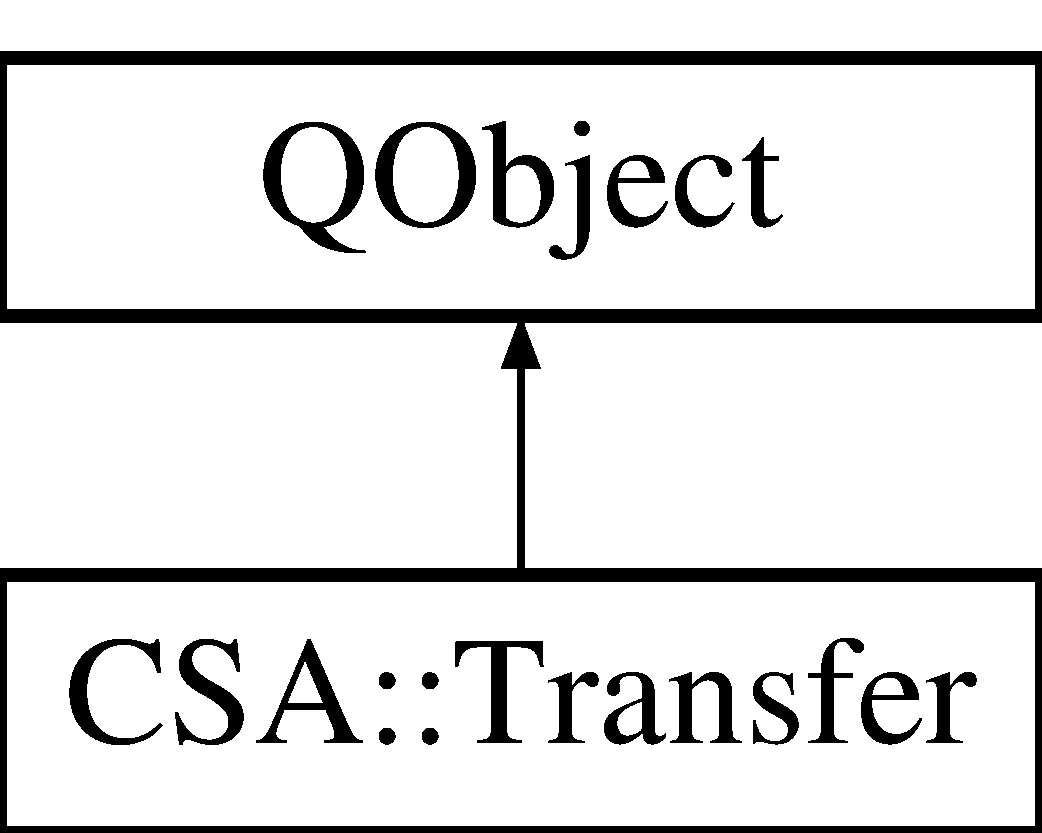
\includegraphics[height=2.000000cm]{classCSA_1_1Transfer}
\end{center}
\end{figure}
\subsection*{Public Types}
\begin{DoxyCompactItemize}
\item 
enum \mbox{\hyperlink{classCSA_1_1Transfer_a827daaa28edc2c4b10ddfa70762355ea}{Type}} \{ \mbox{\hyperlink{classCSA_1_1Transfer_a827daaa28edc2c4b10ddfa70762355eaad5f52d91ac49fd146727f4710767dd08}{Type\+::\+A\+R\+R\+I\+V\+AL}}, 
\mbox{\hyperlink{classCSA_1_1Transfer_a827daaa28edc2c4b10ddfa70762355eaae7cc381a17e714e7ba15ef6f9858304e}{Type\+::\+D\+E\+P\+A\+R\+T\+U\+RE}}, 
\mbox{\hyperlink{classCSA_1_1Transfer_a827daaa28edc2c4b10ddfa70762355eaaeb5ddb3b6096fb90ff720d9c3e2a6628}{Type\+::\+T\+R\+A\+N\+S\+F\+ER}}, 
\mbox{\hyperlink{classCSA_1_1Transfer_a827daaa28edc2c4b10ddfa70762355eaaccc0377a8afbf50e7094f5c23a8af223}{Type\+::\+I\+N\+V\+A\+L\+ID}}
 \}
\end{DoxyCompactItemize}
\subsection*{Signals}
\begin{DoxyCompactItemize}
\item 
void \mbox{\hyperlink{classCSA_1_1Transfer_a6bf33c893850532081dd563cead50e71}{departure\+Leg\+Changed}} ()
\item 
void \mbox{\hyperlink{classCSA_1_1Transfer_ae000de6c0ce8829c7da6a963d9d705ba}{arrival\+Leg\+Changed}} ()
\item 
void \mbox{\hyperlink{classCSA_1_1Transfer_aa7bd4b7ccdba500719b18b0e0f534cb3}{departure\+Changed}} ()
\item 
void \mbox{\hyperlink{classCSA_1_1Transfer_aea7072a6fe1de31c0c783539a879ef73}{arrival\+Changed}} ()
\item 
void \mbox{\hyperlink{classCSA_1_1Transfer_ae404455a073e9bbd3d10fa513c284bb4}{type\+Changed}} ()
\end{DoxyCompactItemize}
\subsection*{Public Member Functions}
\begin{DoxyCompactItemize}
\item 
\mbox{\hyperlink{classCSA_1_1Transfer_a899f767d520735fccc3389da77d8f7ae}{Transfer}} (\mbox{\hyperlink{classCSA_1_1RouteLeg}{C\+S\+A\+::\+Route\+Leg}} $\ast$\mbox{\hyperlink{classCSA_1_1Transfer_a7f2d02a0a1fe7ca96f57fc7864ebfdb8}{departure\+Leg}}=nullptr, \mbox{\hyperlink{classCSA_1_1RouteLeg}{C\+S\+A\+::\+Route\+Leg}} $\ast$\mbox{\hyperlink{classCSA_1_1Transfer_acf5d711e3c206ff0da0cae8146a08beb}{arrival\+Leg}}=nullptr, Q\+Object $\ast$parent=nullptr)
\item 
\mbox{\hyperlink{classCSA_1_1RouteLeg}{C\+S\+A\+::\+Route\+Leg}} $\ast$ \mbox{\hyperlink{classCSA_1_1Transfer_a7f2d02a0a1fe7ca96f57fc7864ebfdb8}{departure\+Leg}} () const
\item 
void \mbox{\hyperlink{classCSA_1_1Transfer_a70a78662a0ef74bb5d88b7796130f001}{set\+Departure\+Leg}} (\mbox{\hyperlink{classCSA_1_1RouteLeg}{C\+S\+A\+::\+Route\+Leg}} $\ast$\mbox{\hyperlink{classCSA_1_1Transfer_a7f2d02a0a1fe7ca96f57fc7864ebfdb8}{departure\+Leg}})
\item 
\mbox{\hyperlink{classCSA_1_1RouteLeg}{C\+S\+A\+::\+Route\+Leg}} $\ast$ \mbox{\hyperlink{classCSA_1_1Transfer_acf5d711e3c206ff0da0cae8146a08beb}{arrival\+Leg}} () const
\item 
void \mbox{\hyperlink{classCSA_1_1Transfer_a3143da004508fa9c75e265054001e7bf}{set\+Arrival\+Leg}} (\mbox{\hyperlink{classCSA_1_1RouteLeg}{C\+S\+A\+::\+Route\+Leg}} $\ast$\mbox{\hyperlink{classCSA_1_1Transfer_acf5d711e3c206ff0da0cae8146a08beb}{arrival\+Leg}})
\item 
\mbox{\hyperlink{classCSA_1_1RouteLegEnd}{C\+S\+A\+::\+Route\+Leg\+End}} $\ast$ \mbox{\hyperlink{classCSA_1_1Transfer_a1442b93dece142706ed8657f1fa9e093}{departure}} () const
\item 
void \mbox{\hyperlink{classCSA_1_1Transfer_a284812274e48e89abae09e8ab37e5670}{set\+Departure}} (\mbox{\hyperlink{classCSA_1_1RouteLegEnd}{C\+S\+A\+::\+Route\+Leg\+End}} $\ast$\mbox{\hyperlink{classCSA_1_1Transfer_a1442b93dece142706ed8657f1fa9e093}{departure}})
\item 
\mbox{\hyperlink{classCSA_1_1RouteLegEnd}{C\+S\+A\+::\+Route\+Leg\+End}} $\ast$ \mbox{\hyperlink{classCSA_1_1Transfer_a1b651e08402cf33cf12d65ad9b6f8011}{arrival}} () const
\item 
void \mbox{\hyperlink{classCSA_1_1Transfer_a0d139f6475fc5d791cf24e964777d9a5}{set\+Arrival}} (\mbox{\hyperlink{classCSA_1_1RouteLegEnd}{C\+S\+A\+::\+Route\+Leg\+End}} $\ast$\mbox{\hyperlink{classCSA_1_1Transfer_a1b651e08402cf33cf12d65ad9b6f8011}{arrival}})
\item 
\mbox{\hyperlink{classCSA_1_1Transfer_a827daaa28edc2c4b10ddfa70762355ea}{C\+S\+A\+::\+Transfer\+::\+Type}} \mbox{\hyperlink{classCSA_1_1Transfer_a52d56463fa87816353419a55cc3753de}{type}} () const
\item 
void \mbox{\hyperlink{classCSA_1_1Transfer_a56fb2f1effd38b42800ba341c15564a5}{set\+Type}} (const \mbox{\hyperlink{classCSA_1_1Transfer_a827daaa28edc2c4b10ddfa70762355ea}{C\+S\+A\+::\+Transfer\+::\+Type}} \&\mbox{\hyperlink{classCSA_1_1Transfer_a52d56463fa87816353419a55cc3753de}{type}})
\item 
Q\+Url \mbox{\hyperlink{classCSA_1_1Transfer_a0878390aa8e48d679b4ceae14cdfd6d7}{uri}} () const
\item 
\mbox{\hyperlink{classCSA_1_1Station}{C\+S\+A\+::\+Station}} $\ast$ \mbox{\hyperlink{classCSA_1_1Transfer_a345bb6fed54db1a5ed9ca8292ab4a57a}{station}} () const
\item 
Q\+Date\+Time \mbox{\hyperlink{classCSA_1_1Transfer_a260cf9330952c162d943d65deffcf5bc}{time}} () const
\item 
qint16 \mbox{\hyperlink{classCSA_1_1Transfer_af2447a3224c016dbb36905b87db0a31e}{delay}} () const
\item 
Q\+Date\+Time \mbox{\hyperlink{classCSA_1_1Transfer_acd43c880d4964a65cf148d0128a7224e}{delayed\+Time}} () const
\item 
Q\+String \mbox{\hyperlink{classCSA_1_1Transfer_a6b3d8d41cbe77793366243ac6902766f}{platform}} () const
\item 
bool \mbox{\hyperlink{classCSA_1_1Transfer_acd29a86e4dbb281ded35cb4e3f9f3000}{is\+Canceled}} () const
\item 
bool \mbox{\hyperlink{classCSA_1_1Transfer_a007baf97e02698d23c86b9c0a6b32350}{is\+Normal\+Platform}} () const
\item 
bool \mbox{\hyperlink{classCSA_1_1Transfer_a7ef5bea75d092ec379d21f5329766343}{is\+Passed}} () const
\item 
\mbox{\hyperlink{classCSA_1_1Vehicle_a331cc81107e5f0a8f37f894729dd9bda}{C\+S\+A\+::\+Vehicle\+::\+Occupancy\+Level}} \mbox{\hyperlink{classCSA_1_1Transfer_a7d5855f37a04c5e0dab60d87ef38f2ef}{occupancy\+Level}} () const
\end{DoxyCompactItemize}
\subsection*{Private Attributes}
\begin{DoxyCompactItemize}
\item 
\mbox{\hyperlink{classCSA_1_1RouteLeg}{C\+S\+A\+::\+Route\+Leg}} $\ast$ \mbox{\hyperlink{classCSA_1_1Transfer_afa7316db40bb5467407ea4cf564e2bc8}{m\+\_\+departure\+Leg}}
\item 
\mbox{\hyperlink{classCSA_1_1RouteLeg}{C\+S\+A\+::\+Route\+Leg}} $\ast$ \mbox{\hyperlink{classCSA_1_1Transfer_a744932ae13de04fdf196f3ab82195521}{m\+\_\+arrival\+Leg}}
\item 
\mbox{\hyperlink{classCSA_1_1RouteLegEnd}{C\+S\+A\+::\+Route\+Leg\+End}} $\ast$ \mbox{\hyperlink{classCSA_1_1Transfer_a5cbccf660e2eeb3235d43fae553b6143}{m\+\_\+departure}}
\item 
\mbox{\hyperlink{classCSA_1_1RouteLegEnd}{C\+S\+A\+::\+Route\+Leg\+End}} $\ast$ \mbox{\hyperlink{classCSA_1_1Transfer_af073c99651592dd83611889e1d1b7677}{m\+\_\+arrival}}
\item 
\mbox{\hyperlink{classCSA_1_1Transfer_a827daaa28edc2c4b10ddfa70762355ea}{C\+S\+A\+::\+Transfer\+::\+Type}} \mbox{\hyperlink{classCSA_1_1Transfer_a491227791f327d6a2a19ce6e91db37f6}{m\+\_\+type}}
\end{DoxyCompactItemize}


\subsection{Member Enumeration Documentation}
\mbox{\Hypertarget{classCSA_1_1Transfer_a827daaa28edc2c4b10ddfa70762355ea}\label{classCSA_1_1Transfer_a827daaa28edc2c4b10ddfa70762355ea}} 
\index{C\+S\+A\+::\+Transfer@{C\+S\+A\+::\+Transfer}!Type@{Type}}
\index{Type@{Type}!C\+S\+A\+::\+Transfer@{C\+S\+A\+::\+Transfer}}
\subsubsection{\texorpdfstring{Type}{Type}}
{\footnotesize\ttfamily enum \mbox{\hyperlink{classCSA_1_1Transfer_a827daaa28edc2c4b10ddfa70762355ea}{C\+S\+A\+::\+Transfer\+::\+Type}}\hspace{0.3cm}{\ttfamily [strong]}}

\begin{DoxyEnumFields}{Enumerator}
\raisebox{\heightof{T}}[0pt][0pt]{\index{A\+R\+R\+I\+V\+AL@{A\+R\+R\+I\+V\+AL}!C\+S\+A\+::\+Transfer@{C\+S\+A\+::\+Transfer}}\index{C\+S\+A\+::\+Transfer@{C\+S\+A\+::\+Transfer}!A\+R\+R\+I\+V\+AL@{A\+R\+R\+I\+V\+AL}}}\mbox{\Hypertarget{classCSA_1_1Transfer_a827daaa28edc2c4b10ddfa70762355eaad5f52d91ac49fd146727f4710767dd08}\label{classCSA_1_1Transfer_a827daaa28edc2c4b10ddfa70762355eaad5f52d91ac49fd146727f4710767dd08}} 
A\+R\+R\+I\+V\+AL&\\
\hline

\raisebox{\heightof{T}}[0pt][0pt]{\index{D\+E\+P\+A\+R\+T\+U\+RE@{D\+E\+P\+A\+R\+T\+U\+RE}!C\+S\+A\+::\+Transfer@{C\+S\+A\+::\+Transfer}}\index{C\+S\+A\+::\+Transfer@{C\+S\+A\+::\+Transfer}!D\+E\+P\+A\+R\+T\+U\+RE@{D\+E\+P\+A\+R\+T\+U\+RE}}}\mbox{\Hypertarget{classCSA_1_1Transfer_a827daaa28edc2c4b10ddfa70762355eaae7cc381a17e714e7ba15ef6f9858304e}\label{classCSA_1_1Transfer_a827daaa28edc2c4b10ddfa70762355eaae7cc381a17e714e7ba15ef6f9858304e}} 
D\+E\+P\+A\+R\+T\+U\+RE&\\
\hline

\raisebox{\heightof{T}}[0pt][0pt]{\index{T\+R\+A\+N\+S\+F\+ER@{T\+R\+A\+N\+S\+F\+ER}!C\+S\+A\+::\+Transfer@{C\+S\+A\+::\+Transfer}}\index{C\+S\+A\+::\+Transfer@{C\+S\+A\+::\+Transfer}!T\+R\+A\+N\+S\+F\+ER@{T\+R\+A\+N\+S\+F\+ER}}}\mbox{\Hypertarget{classCSA_1_1Transfer_a827daaa28edc2c4b10ddfa70762355eaaeb5ddb3b6096fb90ff720d9c3e2a6628}\label{classCSA_1_1Transfer_a827daaa28edc2c4b10ddfa70762355eaaeb5ddb3b6096fb90ff720d9c3e2a6628}} 
T\+R\+A\+N\+S\+F\+ER&\\
\hline

\raisebox{\heightof{T}}[0pt][0pt]{\index{I\+N\+V\+A\+L\+ID@{I\+N\+V\+A\+L\+ID}!C\+S\+A\+::\+Transfer@{C\+S\+A\+::\+Transfer}}\index{C\+S\+A\+::\+Transfer@{C\+S\+A\+::\+Transfer}!I\+N\+V\+A\+L\+ID@{I\+N\+V\+A\+L\+ID}}}\mbox{\Hypertarget{classCSA_1_1Transfer_a827daaa28edc2c4b10ddfa70762355eaaccc0377a8afbf50e7094f5c23a8af223}\label{classCSA_1_1Transfer_a827daaa28edc2c4b10ddfa70762355eaaccc0377a8afbf50e7094f5c23a8af223}} 
I\+N\+V\+A\+L\+ID&\\
\hline

\end{DoxyEnumFields}


\subsection{Constructor \& Destructor Documentation}
\mbox{\Hypertarget{classCSA_1_1Transfer_a899f767d520735fccc3389da77d8f7ae}\label{classCSA_1_1Transfer_a899f767d520735fccc3389da77d8f7ae}} 
\index{C\+S\+A\+::\+Transfer@{C\+S\+A\+::\+Transfer}!Transfer@{Transfer}}
\index{Transfer@{Transfer}!C\+S\+A\+::\+Transfer@{C\+S\+A\+::\+Transfer}}
\subsubsection{\texorpdfstring{Transfer()}{Transfer()}}
{\footnotesize\ttfamily C\+S\+A\+::\+Transfer\+::\+Transfer (\begin{DoxyParamCaption}\item[{\mbox{\hyperlink{classCSA_1_1RouteLeg}{C\+S\+A\+::\+Route\+Leg}} $\ast$}]{departure\+Leg = {\ttfamily nullptr},  }\item[{\mbox{\hyperlink{classCSA_1_1RouteLeg}{C\+S\+A\+::\+Route\+Leg}} $\ast$}]{arrival\+Leg = {\ttfamily nullptr},  }\item[{Q\+Object $\ast$}]{parent = {\ttfamily nullptr} }\end{DoxyParamCaption})\hspace{0.3cm}{\ttfamily [explicit]}}



\subsection{Member Function Documentation}
\mbox{\Hypertarget{classCSA_1_1Transfer_a1b651e08402cf33cf12d65ad9b6f8011}\label{classCSA_1_1Transfer_a1b651e08402cf33cf12d65ad9b6f8011}} 
\index{C\+S\+A\+::\+Transfer@{C\+S\+A\+::\+Transfer}!arrival@{arrival}}
\index{arrival@{arrival}!C\+S\+A\+::\+Transfer@{C\+S\+A\+::\+Transfer}}
\subsubsection{\texorpdfstring{arrival()}{arrival()}}
{\footnotesize\ttfamily \mbox{\hyperlink{classCSA_1_1RouteLegEnd}{C\+S\+A\+::\+Route\+Leg\+End}} $\ast$ C\+S\+A\+::\+Transfer\+::arrival (\begin{DoxyParamCaption}{ }\end{DoxyParamCaption}) const}

\mbox{\Hypertarget{classCSA_1_1Transfer_aea7072a6fe1de31c0c783539a879ef73}\label{classCSA_1_1Transfer_aea7072a6fe1de31c0c783539a879ef73}} 
\index{C\+S\+A\+::\+Transfer@{C\+S\+A\+::\+Transfer}!arrival\+Changed@{arrival\+Changed}}
\index{arrival\+Changed@{arrival\+Changed}!C\+S\+A\+::\+Transfer@{C\+S\+A\+::\+Transfer}}
\subsubsection{\texorpdfstring{arrival\+Changed}{arrivalChanged}}
{\footnotesize\ttfamily void C\+S\+A\+::\+Transfer\+::arrival\+Changed (\begin{DoxyParamCaption}{ }\end{DoxyParamCaption})\hspace{0.3cm}{\ttfamily [signal]}}

\mbox{\Hypertarget{classCSA_1_1Transfer_acf5d711e3c206ff0da0cae8146a08beb}\label{classCSA_1_1Transfer_acf5d711e3c206ff0da0cae8146a08beb}} 
\index{C\+S\+A\+::\+Transfer@{C\+S\+A\+::\+Transfer}!arrival\+Leg@{arrival\+Leg}}
\index{arrival\+Leg@{arrival\+Leg}!C\+S\+A\+::\+Transfer@{C\+S\+A\+::\+Transfer}}
\subsubsection{\texorpdfstring{arrival\+Leg()}{arrivalLeg()}}
{\footnotesize\ttfamily \mbox{\hyperlink{classCSA_1_1RouteLeg}{C\+S\+A\+::\+Route\+Leg}} $\ast$ C\+S\+A\+::\+Transfer\+::arrival\+Leg (\begin{DoxyParamCaption}{ }\end{DoxyParamCaption}) const}

\mbox{\Hypertarget{classCSA_1_1Transfer_ae000de6c0ce8829c7da6a963d9d705ba}\label{classCSA_1_1Transfer_ae000de6c0ce8829c7da6a963d9d705ba}} 
\index{C\+S\+A\+::\+Transfer@{C\+S\+A\+::\+Transfer}!arrival\+Leg\+Changed@{arrival\+Leg\+Changed}}
\index{arrival\+Leg\+Changed@{arrival\+Leg\+Changed}!C\+S\+A\+::\+Transfer@{C\+S\+A\+::\+Transfer}}
\subsubsection{\texorpdfstring{arrival\+Leg\+Changed}{arrivalLegChanged}}
{\footnotesize\ttfamily void C\+S\+A\+::\+Transfer\+::arrival\+Leg\+Changed (\begin{DoxyParamCaption}{ }\end{DoxyParamCaption})\hspace{0.3cm}{\ttfamily [signal]}}

\mbox{\Hypertarget{classCSA_1_1Transfer_af2447a3224c016dbb36905b87db0a31e}\label{classCSA_1_1Transfer_af2447a3224c016dbb36905b87db0a31e}} 
\index{C\+S\+A\+::\+Transfer@{C\+S\+A\+::\+Transfer}!delay@{delay}}
\index{delay@{delay}!C\+S\+A\+::\+Transfer@{C\+S\+A\+::\+Transfer}}
\subsubsection{\texorpdfstring{delay()}{delay()}}
{\footnotesize\ttfamily qint16 C\+S\+A\+::\+Transfer\+::delay (\begin{DoxyParamCaption}{ }\end{DoxyParamCaption}) const}

\mbox{\Hypertarget{classCSA_1_1Transfer_acd43c880d4964a65cf148d0128a7224e}\label{classCSA_1_1Transfer_acd43c880d4964a65cf148d0128a7224e}} 
\index{C\+S\+A\+::\+Transfer@{C\+S\+A\+::\+Transfer}!delayed\+Time@{delayed\+Time}}
\index{delayed\+Time@{delayed\+Time}!C\+S\+A\+::\+Transfer@{C\+S\+A\+::\+Transfer}}
\subsubsection{\texorpdfstring{delayed\+Time()}{delayedTime()}}
{\footnotesize\ttfamily Q\+Date\+Time C\+S\+A\+::\+Transfer\+::delayed\+Time (\begin{DoxyParamCaption}{ }\end{DoxyParamCaption}) const}

\mbox{\Hypertarget{classCSA_1_1Transfer_a1442b93dece142706ed8657f1fa9e093}\label{classCSA_1_1Transfer_a1442b93dece142706ed8657f1fa9e093}} 
\index{C\+S\+A\+::\+Transfer@{C\+S\+A\+::\+Transfer}!departure@{departure}}
\index{departure@{departure}!C\+S\+A\+::\+Transfer@{C\+S\+A\+::\+Transfer}}
\subsubsection{\texorpdfstring{departure()}{departure()}}
{\footnotesize\ttfamily \mbox{\hyperlink{classCSA_1_1RouteLegEnd}{C\+S\+A\+::\+Route\+Leg\+End}} $\ast$ C\+S\+A\+::\+Transfer\+::departure (\begin{DoxyParamCaption}{ }\end{DoxyParamCaption}) const}

\mbox{\Hypertarget{classCSA_1_1Transfer_aa7bd4b7ccdba500719b18b0e0f534cb3}\label{classCSA_1_1Transfer_aa7bd4b7ccdba500719b18b0e0f534cb3}} 
\index{C\+S\+A\+::\+Transfer@{C\+S\+A\+::\+Transfer}!departure\+Changed@{departure\+Changed}}
\index{departure\+Changed@{departure\+Changed}!C\+S\+A\+::\+Transfer@{C\+S\+A\+::\+Transfer}}
\subsubsection{\texorpdfstring{departure\+Changed}{departureChanged}}
{\footnotesize\ttfamily void C\+S\+A\+::\+Transfer\+::departure\+Changed (\begin{DoxyParamCaption}{ }\end{DoxyParamCaption})\hspace{0.3cm}{\ttfamily [signal]}}

\mbox{\Hypertarget{classCSA_1_1Transfer_a7f2d02a0a1fe7ca96f57fc7864ebfdb8}\label{classCSA_1_1Transfer_a7f2d02a0a1fe7ca96f57fc7864ebfdb8}} 
\index{C\+S\+A\+::\+Transfer@{C\+S\+A\+::\+Transfer}!departure\+Leg@{departure\+Leg}}
\index{departure\+Leg@{departure\+Leg}!C\+S\+A\+::\+Transfer@{C\+S\+A\+::\+Transfer}}
\subsubsection{\texorpdfstring{departure\+Leg()}{departureLeg()}}
{\footnotesize\ttfamily \mbox{\hyperlink{classCSA_1_1RouteLeg}{C\+S\+A\+::\+Route\+Leg}} $\ast$ C\+S\+A\+::\+Transfer\+::departure\+Leg (\begin{DoxyParamCaption}{ }\end{DoxyParamCaption}) const}

\mbox{\Hypertarget{classCSA_1_1Transfer_a6bf33c893850532081dd563cead50e71}\label{classCSA_1_1Transfer_a6bf33c893850532081dd563cead50e71}} 
\index{C\+S\+A\+::\+Transfer@{C\+S\+A\+::\+Transfer}!departure\+Leg\+Changed@{departure\+Leg\+Changed}}
\index{departure\+Leg\+Changed@{departure\+Leg\+Changed}!C\+S\+A\+::\+Transfer@{C\+S\+A\+::\+Transfer}}
\subsubsection{\texorpdfstring{departure\+Leg\+Changed}{departureLegChanged}}
{\footnotesize\ttfamily void C\+S\+A\+::\+Transfer\+::departure\+Leg\+Changed (\begin{DoxyParamCaption}{ }\end{DoxyParamCaption})\hspace{0.3cm}{\ttfamily [signal]}}

\mbox{\Hypertarget{classCSA_1_1Transfer_acd29a86e4dbb281ded35cb4e3f9f3000}\label{classCSA_1_1Transfer_acd29a86e4dbb281ded35cb4e3f9f3000}} 
\index{C\+S\+A\+::\+Transfer@{C\+S\+A\+::\+Transfer}!is\+Canceled@{is\+Canceled}}
\index{is\+Canceled@{is\+Canceled}!C\+S\+A\+::\+Transfer@{C\+S\+A\+::\+Transfer}}
\subsubsection{\texorpdfstring{is\+Canceled()}{isCanceled()}}
{\footnotesize\ttfamily bool C\+S\+A\+::\+Transfer\+::is\+Canceled (\begin{DoxyParamCaption}{ }\end{DoxyParamCaption}) const}

\mbox{\Hypertarget{classCSA_1_1Transfer_a007baf97e02698d23c86b9c0a6b32350}\label{classCSA_1_1Transfer_a007baf97e02698d23c86b9c0a6b32350}} 
\index{C\+S\+A\+::\+Transfer@{C\+S\+A\+::\+Transfer}!is\+Normal\+Platform@{is\+Normal\+Platform}}
\index{is\+Normal\+Platform@{is\+Normal\+Platform}!C\+S\+A\+::\+Transfer@{C\+S\+A\+::\+Transfer}}
\subsubsection{\texorpdfstring{is\+Normal\+Platform()}{isNormalPlatform()}}
{\footnotesize\ttfamily bool C\+S\+A\+::\+Transfer\+::is\+Normal\+Platform (\begin{DoxyParamCaption}{ }\end{DoxyParamCaption}) const}

\mbox{\Hypertarget{classCSA_1_1Transfer_a7ef5bea75d092ec379d21f5329766343}\label{classCSA_1_1Transfer_a7ef5bea75d092ec379d21f5329766343}} 
\index{C\+S\+A\+::\+Transfer@{C\+S\+A\+::\+Transfer}!is\+Passed@{is\+Passed}}
\index{is\+Passed@{is\+Passed}!C\+S\+A\+::\+Transfer@{C\+S\+A\+::\+Transfer}}
\subsubsection{\texorpdfstring{is\+Passed()}{isPassed()}}
{\footnotesize\ttfamily bool C\+S\+A\+::\+Transfer\+::is\+Passed (\begin{DoxyParamCaption}{ }\end{DoxyParamCaption}) const}

\mbox{\Hypertarget{classCSA_1_1Transfer_a7d5855f37a04c5e0dab60d87ef38f2ef}\label{classCSA_1_1Transfer_a7d5855f37a04c5e0dab60d87ef38f2ef}} 
\index{C\+S\+A\+::\+Transfer@{C\+S\+A\+::\+Transfer}!occupancy\+Level@{occupancy\+Level}}
\index{occupancy\+Level@{occupancy\+Level}!C\+S\+A\+::\+Transfer@{C\+S\+A\+::\+Transfer}}
\subsubsection{\texorpdfstring{occupancy\+Level()}{occupancyLevel()}}
{\footnotesize\ttfamily \mbox{\hyperlink{classCSA_1_1Vehicle_a331cc81107e5f0a8f37f894729dd9bda}{C\+S\+A\+::\+Vehicle\+::\+Occupancy\+Level}} C\+S\+A\+::\+Transfer\+::occupancy\+Level (\begin{DoxyParamCaption}{ }\end{DoxyParamCaption}) const}

\mbox{\Hypertarget{classCSA_1_1Transfer_a6b3d8d41cbe77793366243ac6902766f}\label{classCSA_1_1Transfer_a6b3d8d41cbe77793366243ac6902766f}} 
\index{C\+S\+A\+::\+Transfer@{C\+S\+A\+::\+Transfer}!platform@{platform}}
\index{platform@{platform}!C\+S\+A\+::\+Transfer@{C\+S\+A\+::\+Transfer}}
\subsubsection{\texorpdfstring{platform()}{platform()}}
{\footnotesize\ttfamily Q\+String C\+S\+A\+::\+Transfer\+::platform (\begin{DoxyParamCaption}{ }\end{DoxyParamCaption}) const}

\mbox{\Hypertarget{classCSA_1_1Transfer_a0d139f6475fc5d791cf24e964777d9a5}\label{classCSA_1_1Transfer_a0d139f6475fc5d791cf24e964777d9a5}} 
\index{C\+S\+A\+::\+Transfer@{C\+S\+A\+::\+Transfer}!set\+Arrival@{set\+Arrival}}
\index{set\+Arrival@{set\+Arrival}!C\+S\+A\+::\+Transfer@{C\+S\+A\+::\+Transfer}}
\subsubsection{\texorpdfstring{set\+Arrival()}{setArrival()}}
{\footnotesize\ttfamily void C\+S\+A\+::\+Transfer\+::set\+Arrival (\begin{DoxyParamCaption}\item[{\mbox{\hyperlink{classCSA_1_1RouteLegEnd}{C\+S\+A\+::\+Route\+Leg\+End}} $\ast$}]{arrival }\end{DoxyParamCaption})}

\mbox{\Hypertarget{classCSA_1_1Transfer_a3143da004508fa9c75e265054001e7bf}\label{classCSA_1_1Transfer_a3143da004508fa9c75e265054001e7bf}} 
\index{C\+S\+A\+::\+Transfer@{C\+S\+A\+::\+Transfer}!set\+Arrival\+Leg@{set\+Arrival\+Leg}}
\index{set\+Arrival\+Leg@{set\+Arrival\+Leg}!C\+S\+A\+::\+Transfer@{C\+S\+A\+::\+Transfer}}
\subsubsection{\texorpdfstring{set\+Arrival\+Leg()}{setArrivalLeg()}}
{\footnotesize\ttfamily void C\+S\+A\+::\+Transfer\+::set\+Arrival\+Leg (\begin{DoxyParamCaption}\item[{\mbox{\hyperlink{classCSA_1_1RouteLeg}{C\+S\+A\+::\+Route\+Leg}} $\ast$}]{arrival\+Leg }\end{DoxyParamCaption})}

\mbox{\Hypertarget{classCSA_1_1Transfer_a284812274e48e89abae09e8ab37e5670}\label{classCSA_1_1Transfer_a284812274e48e89abae09e8ab37e5670}} 
\index{C\+S\+A\+::\+Transfer@{C\+S\+A\+::\+Transfer}!set\+Departure@{set\+Departure}}
\index{set\+Departure@{set\+Departure}!C\+S\+A\+::\+Transfer@{C\+S\+A\+::\+Transfer}}
\subsubsection{\texorpdfstring{set\+Departure()}{setDeparture()}}
{\footnotesize\ttfamily void C\+S\+A\+::\+Transfer\+::set\+Departure (\begin{DoxyParamCaption}\item[{\mbox{\hyperlink{classCSA_1_1RouteLegEnd}{C\+S\+A\+::\+Route\+Leg\+End}} $\ast$}]{departure }\end{DoxyParamCaption})}

\mbox{\Hypertarget{classCSA_1_1Transfer_a70a78662a0ef74bb5d88b7796130f001}\label{classCSA_1_1Transfer_a70a78662a0ef74bb5d88b7796130f001}} 
\index{C\+S\+A\+::\+Transfer@{C\+S\+A\+::\+Transfer}!set\+Departure\+Leg@{set\+Departure\+Leg}}
\index{set\+Departure\+Leg@{set\+Departure\+Leg}!C\+S\+A\+::\+Transfer@{C\+S\+A\+::\+Transfer}}
\subsubsection{\texorpdfstring{set\+Departure\+Leg()}{setDepartureLeg()}}
{\footnotesize\ttfamily void C\+S\+A\+::\+Transfer\+::set\+Departure\+Leg (\begin{DoxyParamCaption}\item[{\mbox{\hyperlink{classCSA_1_1RouteLeg}{C\+S\+A\+::\+Route\+Leg}} $\ast$}]{departure\+Leg }\end{DoxyParamCaption})}

\mbox{\Hypertarget{classCSA_1_1Transfer_a56fb2f1effd38b42800ba341c15564a5}\label{classCSA_1_1Transfer_a56fb2f1effd38b42800ba341c15564a5}} 
\index{C\+S\+A\+::\+Transfer@{C\+S\+A\+::\+Transfer}!set\+Type@{set\+Type}}
\index{set\+Type@{set\+Type}!C\+S\+A\+::\+Transfer@{C\+S\+A\+::\+Transfer}}
\subsubsection{\texorpdfstring{set\+Type()}{setType()}}
{\footnotesize\ttfamily void C\+S\+A\+::\+Transfer\+::set\+Type (\begin{DoxyParamCaption}\item[{const \mbox{\hyperlink{classCSA_1_1Transfer_a827daaa28edc2c4b10ddfa70762355ea}{C\+S\+A\+::\+Transfer\+::\+Type}} \&}]{type }\end{DoxyParamCaption})}

\mbox{\Hypertarget{classCSA_1_1Transfer_a345bb6fed54db1a5ed9ca8292ab4a57a}\label{classCSA_1_1Transfer_a345bb6fed54db1a5ed9ca8292ab4a57a}} 
\index{C\+S\+A\+::\+Transfer@{C\+S\+A\+::\+Transfer}!station@{station}}
\index{station@{station}!C\+S\+A\+::\+Transfer@{C\+S\+A\+::\+Transfer}}
\subsubsection{\texorpdfstring{station()}{station()}}
{\footnotesize\ttfamily \mbox{\hyperlink{classCSA_1_1Station}{C\+S\+A\+::\+Station}} $\ast$ C\+S\+A\+::\+Transfer\+::station (\begin{DoxyParamCaption}{ }\end{DoxyParamCaption}) const}

\mbox{\Hypertarget{classCSA_1_1Transfer_a260cf9330952c162d943d65deffcf5bc}\label{classCSA_1_1Transfer_a260cf9330952c162d943d65deffcf5bc}} 
\index{C\+S\+A\+::\+Transfer@{C\+S\+A\+::\+Transfer}!time@{time}}
\index{time@{time}!C\+S\+A\+::\+Transfer@{C\+S\+A\+::\+Transfer}}
\subsubsection{\texorpdfstring{time()}{time()}}
{\footnotesize\ttfamily Q\+Date\+Time C\+S\+A\+::\+Transfer\+::time (\begin{DoxyParamCaption}{ }\end{DoxyParamCaption}) const}

\mbox{\Hypertarget{classCSA_1_1Transfer_a52d56463fa87816353419a55cc3753de}\label{classCSA_1_1Transfer_a52d56463fa87816353419a55cc3753de}} 
\index{C\+S\+A\+::\+Transfer@{C\+S\+A\+::\+Transfer}!type@{type}}
\index{type@{type}!C\+S\+A\+::\+Transfer@{C\+S\+A\+::\+Transfer}}
\subsubsection{\texorpdfstring{type()}{type()}}
{\footnotesize\ttfamily \mbox{\hyperlink{classCSA_1_1Transfer_a827daaa28edc2c4b10ddfa70762355ea}{C\+S\+A\+::\+Transfer\+::\+Type}} C\+S\+A\+::\+Transfer\+::type (\begin{DoxyParamCaption}{ }\end{DoxyParamCaption}) const}

\mbox{\Hypertarget{classCSA_1_1Transfer_ae404455a073e9bbd3d10fa513c284bb4}\label{classCSA_1_1Transfer_ae404455a073e9bbd3d10fa513c284bb4}} 
\index{C\+S\+A\+::\+Transfer@{C\+S\+A\+::\+Transfer}!type\+Changed@{type\+Changed}}
\index{type\+Changed@{type\+Changed}!C\+S\+A\+::\+Transfer@{C\+S\+A\+::\+Transfer}}
\subsubsection{\texorpdfstring{type\+Changed}{typeChanged}}
{\footnotesize\ttfamily void C\+S\+A\+::\+Transfer\+::type\+Changed (\begin{DoxyParamCaption}{ }\end{DoxyParamCaption})\hspace{0.3cm}{\ttfamily [signal]}}

\mbox{\Hypertarget{classCSA_1_1Transfer_a0878390aa8e48d679b4ceae14cdfd6d7}\label{classCSA_1_1Transfer_a0878390aa8e48d679b4ceae14cdfd6d7}} 
\index{C\+S\+A\+::\+Transfer@{C\+S\+A\+::\+Transfer}!uri@{uri}}
\index{uri@{uri}!C\+S\+A\+::\+Transfer@{C\+S\+A\+::\+Transfer}}
\subsubsection{\texorpdfstring{uri()}{uri()}}
{\footnotesize\ttfamily Q\+Url C\+S\+A\+::\+Transfer\+::uri (\begin{DoxyParamCaption}{ }\end{DoxyParamCaption}) const}



\subsection{Member Data Documentation}
\mbox{\Hypertarget{classCSA_1_1Transfer_af073c99651592dd83611889e1d1b7677}\label{classCSA_1_1Transfer_af073c99651592dd83611889e1d1b7677}} 
\index{C\+S\+A\+::\+Transfer@{C\+S\+A\+::\+Transfer}!m\+\_\+arrival@{m\+\_\+arrival}}
\index{m\+\_\+arrival@{m\+\_\+arrival}!C\+S\+A\+::\+Transfer@{C\+S\+A\+::\+Transfer}}
\subsubsection{\texorpdfstring{m\+\_\+arrival}{m\_arrival}}
{\footnotesize\ttfamily \mbox{\hyperlink{classCSA_1_1RouteLegEnd}{C\+S\+A\+::\+Route\+Leg\+End}}$\ast$ C\+S\+A\+::\+Transfer\+::m\+\_\+arrival\hspace{0.3cm}{\ttfamily [private]}}

\mbox{\Hypertarget{classCSA_1_1Transfer_a744932ae13de04fdf196f3ab82195521}\label{classCSA_1_1Transfer_a744932ae13de04fdf196f3ab82195521}} 
\index{C\+S\+A\+::\+Transfer@{C\+S\+A\+::\+Transfer}!m\+\_\+arrival\+Leg@{m\+\_\+arrival\+Leg}}
\index{m\+\_\+arrival\+Leg@{m\+\_\+arrival\+Leg}!C\+S\+A\+::\+Transfer@{C\+S\+A\+::\+Transfer}}
\subsubsection{\texorpdfstring{m\+\_\+arrival\+Leg}{m\_arrivalLeg}}
{\footnotesize\ttfamily \mbox{\hyperlink{classCSA_1_1RouteLeg}{C\+S\+A\+::\+Route\+Leg}}$\ast$ C\+S\+A\+::\+Transfer\+::m\+\_\+arrival\+Leg\hspace{0.3cm}{\ttfamily [private]}}

\mbox{\Hypertarget{classCSA_1_1Transfer_a5cbccf660e2eeb3235d43fae553b6143}\label{classCSA_1_1Transfer_a5cbccf660e2eeb3235d43fae553b6143}} 
\index{C\+S\+A\+::\+Transfer@{C\+S\+A\+::\+Transfer}!m\+\_\+departure@{m\+\_\+departure}}
\index{m\+\_\+departure@{m\+\_\+departure}!C\+S\+A\+::\+Transfer@{C\+S\+A\+::\+Transfer}}
\subsubsection{\texorpdfstring{m\+\_\+departure}{m\_departure}}
{\footnotesize\ttfamily \mbox{\hyperlink{classCSA_1_1RouteLegEnd}{C\+S\+A\+::\+Route\+Leg\+End}}$\ast$ C\+S\+A\+::\+Transfer\+::m\+\_\+departure\hspace{0.3cm}{\ttfamily [private]}}

\mbox{\Hypertarget{classCSA_1_1Transfer_afa7316db40bb5467407ea4cf564e2bc8}\label{classCSA_1_1Transfer_afa7316db40bb5467407ea4cf564e2bc8}} 
\index{C\+S\+A\+::\+Transfer@{C\+S\+A\+::\+Transfer}!m\+\_\+departure\+Leg@{m\+\_\+departure\+Leg}}
\index{m\+\_\+departure\+Leg@{m\+\_\+departure\+Leg}!C\+S\+A\+::\+Transfer@{C\+S\+A\+::\+Transfer}}
\subsubsection{\texorpdfstring{m\+\_\+departure\+Leg}{m\_departureLeg}}
{\footnotesize\ttfamily \mbox{\hyperlink{classCSA_1_1RouteLeg}{C\+S\+A\+::\+Route\+Leg}}$\ast$ C\+S\+A\+::\+Transfer\+::m\+\_\+departure\+Leg\hspace{0.3cm}{\ttfamily [private]}}

\mbox{\Hypertarget{classCSA_1_1Transfer_a491227791f327d6a2a19ce6e91db37f6}\label{classCSA_1_1Transfer_a491227791f327d6a2a19ce6e91db37f6}} 
\index{C\+S\+A\+::\+Transfer@{C\+S\+A\+::\+Transfer}!m\+\_\+type@{m\+\_\+type}}
\index{m\+\_\+type@{m\+\_\+type}!C\+S\+A\+::\+Transfer@{C\+S\+A\+::\+Transfer}}
\subsubsection{\texorpdfstring{m\+\_\+type}{m\_type}}
{\footnotesize\ttfamily \mbox{\hyperlink{classCSA_1_1Transfer_a827daaa28edc2c4b10ddfa70762355ea}{C\+S\+A\+::\+Transfer\+::\+Type}} C\+S\+A\+::\+Transfer\+::m\+\_\+type\hspace{0.3cm}{\ttfamily [private]}}



The documentation for this class was generated from the following files\+:\begin{DoxyCompactItemize}
\item 
src/linkedconnections/csa/\mbox{\hyperlink{csatransfer_8h}{csatransfer.\+h}}\item 
src/linkedconnections/csa/\mbox{\hyperlink{csatransfer_8cpp}{csatransfer.\+cpp}}\end{DoxyCompactItemize}

\hypertarget{classCSA_1_1Vehicle}{}\section{C\+SA\+:\+:Vehicle Class Reference}
\label{classCSA_1_1Vehicle}\index{C\+S\+A\+::\+Vehicle@{C\+S\+A\+::\+Vehicle}}


{\ttfamily \#include $<$csavehicle.\+h$>$}

Inheritance diagram for C\+SA\+:\+:Vehicle\+:\begin{figure}[H]
\begin{center}
\leavevmode
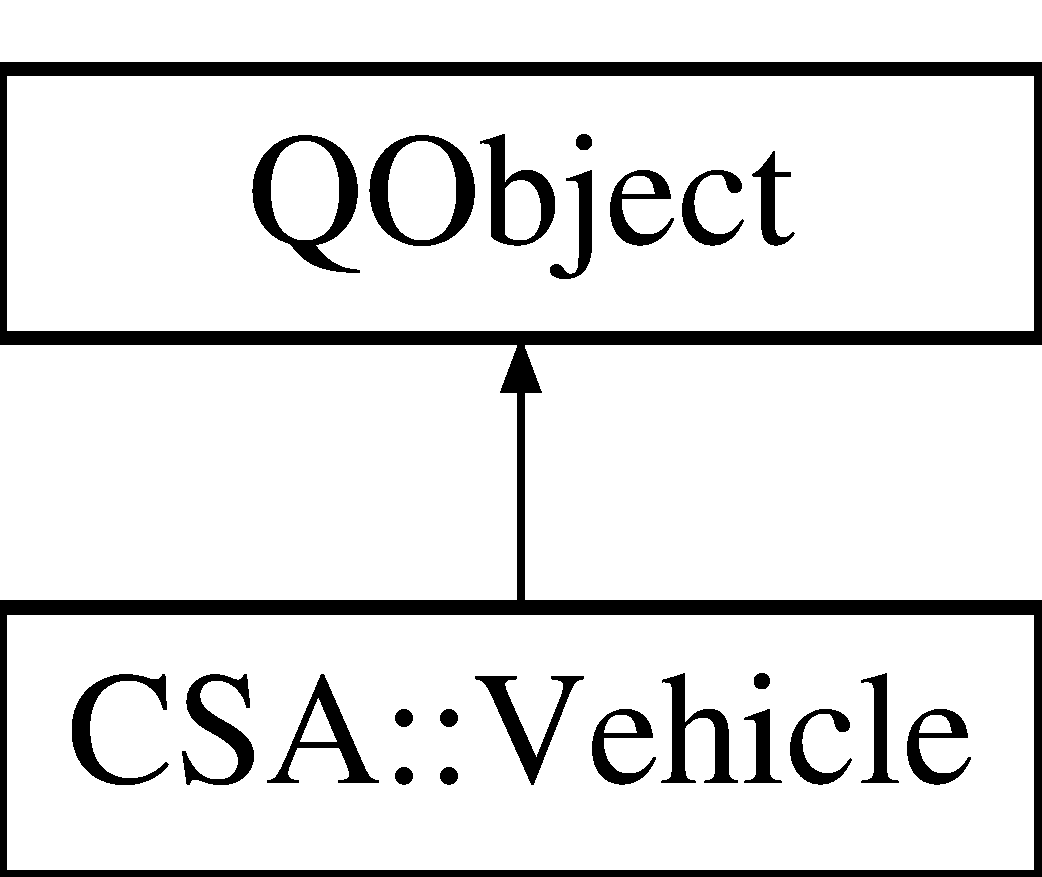
\includegraphics[height=2.000000cm]{classCSA_1_1Vehicle}
\end{center}
\end{figure}
\subsection*{Public Types}
\begin{DoxyCompactItemize}
\item 
enum \mbox{\hyperlink{classCSA_1_1Vehicle_a331cc81107e5f0a8f37f894729dd9bda}{Occupancy\+Level}} \{ \newline
\mbox{\hyperlink{classCSA_1_1Vehicle_a331cc81107e5f0a8f37f894729dd9bdaa40aa75f8e8cfdf7b660c5620e953229f}{Occupancy\+Level\+::\+U\+N\+S\+U\+P\+P\+O\+R\+T\+ED}}, 
\mbox{\hyperlink{classCSA_1_1Vehicle_a331cc81107e5f0a8f37f894729dd9bdaa696b031073e74bf2cb98e5ef201d4aa3}{Occupancy\+Level\+::\+U\+N\+K\+N\+O\+WN}}, 
\mbox{\hyperlink{classCSA_1_1Vehicle_a331cc81107e5f0a8f37f894729dd9bdaa41bc94cbd8eebea13ce0491b2ac11b88}{Occupancy\+Level\+::\+L\+OW}}, 
\mbox{\hyperlink{classCSA_1_1Vehicle_a331cc81107e5f0a8f37f894729dd9bdaac87f3be66ffc3c0d4249f1c2cc5f3cce}{Occupancy\+Level\+::\+M\+E\+D\+I\+UM}}, 
\newline
\mbox{\hyperlink{classCSA_1_1Vehicle_a331cc81107e5f0a8f37f894729dd9bdaab89de3b4b81c4facfac906edf29aec8c}{Occupancy\+Level\+::\+H\+I\+GH}}
 \}
\end{DoxyCompactItemize}
\subsection*{Signals}
\begin{DoxyCompactItemize}
\item 
void \mbox{\hyperlink{classCSA_1_1Vehicle_ab473f2c81f6e0a0894e525466bfac43f}{uri\+Changed}} ()
\item 
void \mbox{\hyperlink{classCSA_1_1Vehicle_a4db7ec27aa6ef10cf09ac41cfabd2642}{id\+Changed}} ()
\item 
void \mbox{\hyperlink{classCSA_1_1Vehicle_a2de3755a1458b3790852b3fd759136b7}{headsign\+Changed}} ()
\end{DoxyCompactItemize}
\subsection*{Public Member Functions}
\begin{DoxyCompactItemize}
\item 
\mbox{\hyperlink{classCSA_1_1Vehicle_a3697b0944b1b62366b0ab4b3011ff60f}{Vehicle}} (const Q\+Url \&\mbox{\hyperlink{classCSA_1_1Vehicle_a580c5dc0cf95552ae0dc20cfdb04d84a}{uri}}, const Q\+Url \&\mbox{\hyperlink{classCSA_1_1Vehicle_a99b2869ea0bee81d0bff5e32259146e6}{id}}, const Q\+String \&\mbox{\hyperlink{classCSA_1_1Vehicle_a7d8e773759fc99129669be053a731e95}{headsign}}, Q\+Object $\ast$parent=nullptr)
\item 
Q\+Url \mbox{\hyperlink{classCSA_1_1Vehicle_a580c5dc0cf95552ae0dc20cfdb04d84a}{uri}} () const
\item 
void \mbox{\hyperlink{classCSA_1_1Vehicle_a8988c6bd084f1385695d73ad80ffd67b}{set\+Uri}} (const Q\+Url \&\mbox{\hyperlink{classCSA_1_1Vehicle_a580c5dc0cf95552ae0dc20cfdb04d84a}{uri}})
\item 
Q\+Url \mbox{\hyperlink{classCSA_1_1Vehicle_a99b2869ea0bee81d0bff5e32259146e6}{id}} () const
\item 
void \mbox{\hyperlink{classCSA_1_1Vehicle_a65c6be2cd36fd59ba454e105452be1ee}{set\+Id}} (const Q\+Url \&\mbox{\hyperlink{classCSA_1_1Vehicle_a99b2869ea0bee81d0bff5e32259146e6}{id}})
\item 
Q\+String \mbox{\hyperlink{classCSA_1_1Vehicle_a7d8e773759fc99129669be053a731e95}{headsign}} () const
\item 
void \mbox{\hyperlink{classCSA_1_1Vehicle_ab47b72449154d72055cf506b6fc9a90a}{set\+Headsign}} (const Q\+String \&\mbox{\hyperlink{classCSA_1_1Vehicle_a7d8e773759fc99129669be053a731e95}{headsign}})
\end{DoxyCompactItemize}
\subsection*{Private Attributes}
\begin{DoxyCompactItemize}
\item 
Q\+Url \mbox{\hyperlink{classCSA_1_1Vehicle_a9ac31c6900099e172d8eae31f04849e4}{m\+\_\+uri}}
\item 
Q\+Url \mbox{\hyperlink{classCSA_1_1Vehicle_ac1d751db24a92a8b38efae09d7759fc8}{m\+\_\+id}}
\item 
Q\+String \mbox{\hyperlink{classCSA_1_1Vehicle_ab6764acaa95b5493b276e28a179952fd}{m\+\_\+headsign}}
\end{DoxyCompactItemize}


\subsection{Member Enumeration Documentation}
\mbox{\Hypertarget{classCSA_1_1Vehicle_a331cc81107e5f0a8f37f894729dd9bda}\label{classCSA_1_1Vehicle_a331cc81107e5f0a8f37f894729dd9bda}} 
\index{C\+S\+A\+::\+Vehicle@{C\+S\+A\+::\+Vehicle}!Occupancy\+Level@{Occupancy\+Level}}
\index{Occupancy\+Level@{Occupancy\+Level}!C\+S\+A\+::\+Vehicle@{C\+S\+A\+::\+Vehicle}}
\subsubsection{\texorpdfstring{Occupancy\+Level}{OccupancyLevel}}
{\footnotesize\ttfamily enum \mbox{\hyperlink{classCSA_1_1Vehicle_a331cc81107e5f0a8f37f894729dd9bda}{C\+S\+A\+::\+Vehicle\+::\+Occupancy\+Level}}\hspace{0.3cm}{\ttfamily [strong]}}

\begin{DoxyEnumFields}{Enumerator}
\raisebox{\heightof{T}}[0pt][0pt]{\index{U\+N\+S\+U\+P\+P\+O\+R\+T\+ED@{U\+N\+S\+U\+P\+P\+O\+R\+T\+ED}!C\+S\+A\+::\+Vehicle@{C\+S\+A\+::\+Vehicle}}\index{C\+S\+A\+::\+Vehicle@{C\+S\+A\+::\+Vehicle}!U\+N\+S\+U\+P\+P\+O\+R\+T\+ED@{U\+N\+S\+U\+P\+P\+O\+R\+T\+ED}}}\mbox{\Hypertarget{classCSA_1_1Vehicle_a331cc81107e5f0a8f37f894729dd9bdaa40aa75f8e8cfdf7b660c5620e953229f}\label{classCSA_1_1Vehicle_a331cc81107e5f0a8f37f894729dd9bdaa40aa75f8e8cfdf7b660c5620e953229f}} 
U\+N\+S\+U\+P\+P\+O\+R\+T\+ED&\\
\hline

\raisebox{\heightof{T}}[0pt][0pt]{\index{U\+N\+K\+N\+O\+WN@{U\+N\+K\+N\+O\+WN}!C\+S\+A\+::\+Vehicle@{C\+S\+A\+::\+Vehicle}}\index{C\+S\+A\+::\+Vehicle@{C\+S\+A\+::\+Vehicle}!U\+N\+K\+N\+O\+WN@{U\+N\+K\+N\+O\+WN}}}\mbox{\Hypertarget{classCSA_1_1Vehicle_a331cc81107e5f0a8f37f894729dd9bdaa696b031073e74bf2cb98e5ef201d4aa3}\label{classCSA_1_1Vehicle_a331cc81107e5f0a8f37f894729dd9bdaa696b031073e74bf2cb98e5ef201d4aa3}} 
U\+N\+K\+N\+O\+WN&\\
\hline

\raisebox{\heightof{T}}[0pt][0pt]{\index{L\+OW@{L\+OW}!C\+S\+A\+::\+Vehicle@{C\+S\+A\+::\+Vehicle}}\index{C\+S\+A\+::\+Vehicle@{C\+S\+A\+::\+Vehicle}!L\+OW@{L\+OW}}}\mbox{\Hypertarget{classCSA_1_1Vehicle_a331cc81107e5f0a8f37f894729dd9bdaa41bc94cbd8eebea13ce0491b2ac11b88}\label{classCSA_1_1Vehicle_a331cc81107e5f0a8f37f894729dd9bdaa41bc94cbd8eebea13ce0491b2ac11b88}} 
L\+OW&\\
\hline

\raisebox{\heightof{T}}[0pt][0pt]{\index{M\+E\+D\+I\+UM@{M\+E\+D\+I\+UM}!C\+S\+A\+::\+Vehicle@{C\+S\+A\+::\+Vehicle}}\index{C\+S\+A\+::\+Vehicle@{C\+S\+A\+::\+Vehicle}!M\+E\+D\+I\+UM@{M\+E\+D\+I\+UM}}}\mbox{\Hypertarget{classCSA_1_1Vehicle_a331cc81107e5f0a8f37f894729dd9bdaac87f3be66ffc3c0d4249f1c2cc5f3cce}\label{classCSA_1_1Vehicle_a331cc81107e5f0a8f37f894729dd9bdaac87f3be66ffc3c0d4249f1c2cc5f3cce}} 
M\+E\+D\+I\+UM&\\
\hline

\raisebox{\heightof{T}}[0pt][0pt]{\index{H\+I\+GH@{H\+I\+GH}!C\+S\+A\+::\+Vehicle@{C\+S\+A\+::\+Vehicle}}\index{C\+S\+A\+::\+Vehicle@{C\+S\+A\+::\+Vehicle}!H\+I\+GH@{H\+I\+GH}}}\mbox{\Hypertarget{classCSA_1_1Vehicle_a331cc81107e5f0a8f37f894729dd9bdaab89de3b4b81c4facfac906edf29aec8c}\label{classCSA_1_1Vehicle_a331cc81107e5f0a8f37f894729dd9bdaab89de3b4b81c4facfac906edf29aec8c}} 
H\+I\+GH&\\
\hline

\end{DoxyEnumFields}


\subsection{Constructor \& Destructor Documentation}
\mbox{\Hypertarget{classCSA_1_1Vehicle_a3697b0944b1b62366b0ab4b3011ff60f}\label{classCSA_1_1Vehicle_a3697b0944b1b62366b0ab4b3011ff60f}} 
\index{C\+S\+A\+::\+Vehicle@{C\+S\+A\+::\+Vehicle}!Vehicle@{Vehicle}}
\index{Vehicle@{Vehicle}!C\+S\+A\+::\+Vehicle@{C\+S\+A\+::\+Vehicle}}
\subsubsection{\texorpdfstring{Vehicle()}{Vehicle()}}
{\footnotesize\ttfamily C\+S\+A\+::\+Vehicle\+::\+Vehicle (\begin{DoxyParamCaption}\item[{const Q\+Url \&}]{uri,  }\item[{const Q\+Url \&}]{id,  }\item[{const Q\+String \&}]{headsign,  }\item[{Q\+Object $\ast$}]{parent = {\ttfamily nullptr} }\end{DoxyParamCaption})\hspace{0.3cm}{\ttfamily [explicit]}}



\subsection{Member Function Documentation}
\mbox{\Hypertarget{classCSA_1_1Vehicle_a7d8e773759fc99129669be053a731e95}\label{classCSA_1_1Vehicle_a7d8e773759fc99129669be053a731e95}} 
\index{C\+S\+A\+::\+Vehicle@{C\+S\+A\+::\+Vehicle}!headsign@{headsign}}
\index{headsign@{headsign}!C\+S\+A\+::\+Vehicle@{C\+S\+A\+::\+Vehicle}}
\subsubsection{\texorpdfstring{headsign()}{headsign()}}
{\footnotesize\ttfamily Q\+String C\+S\+A\+::\+Vehicle\+::headsign (\begin{DoxyParamCaption}{ }\end{DoxyParamCaption}) const}

\mbox{\Hypertarget{classCSA_1_1Vehicle_a2de3755a1458b3790852b3fd759136b7}\label{classCSA_1_1Vehicle_a2de3755a1458b3790852b3fd759136b7}} 
\index{C\+S\+A\+::\+Vehicle@{C\+S\+A\+::\+Vehicle}!headsign\+Changed@{headsign\+Changed}}
\index{headsign\+Changed@{headsign\+Changed}!C\+S\+A\+::\+Vehicle@{C\+S\+A\+::\+Vehicle}}
\subsubsection{\texorpdfstring{headsign\+Changed}{headsignChanged}}
{\footnotesize\ttfamily void C\+S\+A\+::\+Vehicle\+::headsign\+Changed (\begin{DoxyParamCaption}{ }\end{DoxyParamCaption})\hspace{0.3cm}{\ttfamily [signal]}}

\mbox{\Hypertarget{classCSA_1_1Vehicle_a99b2869ea0bee81d0bff5e32259146e6}\label{classCSA_1_1Vehicle_a99b2869ea0bee81d0bff5e32259146e6}} 
\index{C\+S\+A\+::\+Vehicle@{C\+S\+A\+::\+Vehicle}!id@{id}}
\index{id@{id}!C\+S\+A\+::\+Vehicle@{C\+S\+A\+::\+Vehicle}}
\subsubsection{\texorpdfstring{id()}{id()}}
{\footnotesize\ttfamily Q\+Url C\+S\+A\+::\+Vehicle\+::id (\begin{DoxyParamCaption}{ }\end{DoxyParamCaption}) const}

\mbox{\Hypertarget{classCSA_1_1Vehicle_a4db7ec27aa6ef10cf09ac41cfabd2642}\label{classCSA_1_1Vehicle_a4db7ec27aa6ef10cf09ac41cfabd2642}} 
\index{C\+S\+A\+::\+Vehicle@{C\+S\+A\+::\+Vehicle}!id\+Changed@{id\+Changed}}
\index{id\+Changed@{id\+Changed}!C\+S\+A\+::\+Vehicle@{C\+S\+A\+::\+Vehicle}}
\subsubsection{\texorpdfstring{id\+Changed}{idChanged}}
{\footnotesize\ttfamily void C\+S\+A\+::\+Vehicle\+::id\+Changed (\begin{DoxyParamCaption}{ }\end{DoxyParamCaption})\hspace{0.3cm}{\ttfamily [signal]}}

\mbox{\Hypertarget{classCSA_1_1Vehicle_ab47b72449154d72055cf506b6fc9a90a}\label{classCSA_1_1Vehicle_ab47b72449154d72055cf506b6fc9a90a}} 
\index{C\+S\+A\+::\+Vehicle@{C\+S\+A\+::\+Vehicle}!set\+Headsign@{set\+Headsign}}
\index{set\+Headsign@{set\+Headsign}!C\+S\+A\+::\+Vehicle@{C\+S\+A\+::\+Vehicle}}
\subsubsection{\texorpdfstring{set\+Headsign()}{setHeadsign()}}
{\footnotesize\ttfamily void C\+S\+A\+::\+Vehicle\+::set\+Headsign (\begin{DoxyParamCaption}\item[{const Q\+String \&}]{headsign }\end{DoxyParamCaption})}

\mbox{\Hypertarget{classCSA_1_1Vehicle_a65c6be2cd36fd59ba454e105452be1ee}\label{classCSA_1_1Vehicle_a65c6be2cd36fd59ba454e105452be1ee}} 
\index{C\+S\+A\+::\+Vehicle@{C\+S\+A\+::\+Vehicle}!set\+Id@{set\+Id}}
\index{set\+Id@{set\+Id}!C\+S\+A\+::\+Vehicle@{C\+S\+A\+::\+Vehicle}}
\subsubsection{\texorpdfstring{set\+Id()}{setId()}}
{\footnotesize\ttfamily void C\+S\+A\+::\+Vehicle\+::set\+Id (\begin{DoxyParamCaption}\item[{const Q\+Url \&}]{id }\end{DoxyParamCaption})}

\mbox{\Hypertarget{classCSA_1_1Vehicle_a8988c6bd084f1385695d73ad80ffd67b}\label{classCSA_1_1Vehicle_a8988c6bd084f1385695d73ad80ffd67b}} 
\index{C\+S\+A\+::\+Vehicle@{C\+S\+A\+::\+Vehicle}!set\+Uri@{set\+Uri}}
\index{set\+Uri@{set\+Uri}!C\+S\+A\+::\+Vehicle@{C\+S\+A\+::\+Vehicle}}
\subsubsection{\texorpdfstring{set\+Uri()}{setUri()}}
{\footnotesize\ttfamily void C\+S\+A\+::\+Vehicle\+::set\+Uri (\begin{DoxyParamCaption}\item[{const Q\+Url \&}]{uri }\end{DoxyParamCaption})}

\mbox{\Hypertarget{classCSA_1_1Vehicle_a580c5dc0cf95552ae0dc20cfdb04d84a}\label{classCSA_1_1Vehicle_a580c5dc0cf95552ae0dc20cfdb04d84a}} 
\index{C\+S\+A\+::\+Vehicle@{C\+S\+A\+::\+Vehicle}!uri@{uri}}
\index{uri@{uri}!C\+S\+A\+::\+Vehicle@{C\+S\+A\+::\+Vehicle}}
\subsubsection{\texorpdfstring{uri()}{uri()}}
{\footnotesize\ttfamily Q\+Url C\+S\+A\+::\+Vehicle\+::uri (\begin{DoxyParamCaption}{ }\end{DoxyParamCaption}) const}

\mbox{\Hypertarget{classCSA_1_1Vehicle_ab473f2c81f6e0a0894e525466bfac43f}\label{classCSA_1_1Vehicle_ab473f2c81f6e0a0894e525466bfac43f}} 
\index{C\+S\+A\+::\+Vehicle@{C\+S\+A\+::\+Vehicle}!uri\+Changed@{uri\+Changed}}
\index{uri\+Changed@{uri\+Changed}!C\+S\+A\+::\+Vehicle@{C\+S\+A\+::\+Vehicle}}
\subsubsection{\texorpdfstring{uri\+Changed}{uriChanged}}
{\footnotesize\ttfamily void C\+S\+A\+::\+Vehicle\+::uri\+Changed (\begin{DoxyParamCaption}{ }\end{DoxyParamCaption})\hspace{0.3cm}{\ttfamily [signal]}}



\subsection{Member Data Documentation}
\mbox{\Hypertarget{classCSA_1_1Vehicle_ab6764acaa95b5493b276e28a179952fd}\label{classCSA_1_1Vehicle_ab6764acaa95b5493b276e28a179952fd}} 
\index{C\+S\+A\+::\+Vehicle@{C\+S\+A\+::\+Vehicle}!m\+\_\+headsign@{m\+\_\+headsign}}
\index{m\+\_\+headsign@{m\+\_\+headsign}!C\+S\+A\+::\+Vehicle@{C\+S\+A\+::\+Vehicle}}
\subsubsection{\texorpdfstring{m\+\_\+headsign}{m\_headsign}}
{\footnotesize\ttfamily Q\+String C\+S\+A\+::\+Vehicle\+::m\+\_\+headsign\hspace{0.3cm}{\ttfamily [private]}}

\mbox{\Hypertarget{classCSA_1_1Vehicle_ac1d751db24a92a8b38efae09d7759fc8}\label{classCSA_1_1Vehicle_ac1d751db24a92a8b38efae09d7759fc8}} 
\index{C\+S\+A\+::\+Vehicle@{C\+S\+A\+::\+Vehicle}!m\+\_\+id@{m\+\_\+id}}
\index{m\+\_\+id@{m\+\_\+id}!C\+S\+A\+::\+Vehicle@{C\+S\+A\+::\+Vehicle}}
\subsubsection{\texorpdfstring{m\+\_\+id}{m\_id}}
{\footnotesize\ttfamily Q\+Url C\+S\+A\+::\+Vehicle\+::m\+\_\+id\hspace{0.3cm}{\ttfamily [private]}}

\mbox{\Hypertarget{classCSA_1_1Vehicle_a9ac31c6900099e172d8eae31f04849e4}\label{classCSA_1_1Vehicle_a9ac31c6900099e172d8eae31f04849e4}} 
\index{C\+S\+A\+::\+Vehicle@{C\+S\+A\+::\+Vehicle}!m\+\_\+uri@{m\+\_\+uri}}
\index{m\+\_\+uri@{m\+\_\+uri}!C\+S\+A\+::\+Vehicle@{C\+S\+A\+::\+Vehicle}}
\subsubsection{\texorpdfstring{m\+\_\+uri}{m\_uri}}
{\footnotesize\ttfamily Q\+Url C\+S\+A\+::\+Vehicle\+::m\+\_\+uri\hspace{0.3cm}{\ttfamily [private]}}



The documentation for this class was generated from the following files\+:\begin{DoxyCompactItemize}
\item 
src/linkedconnections/csa/\mbox{\hyperlink{csavehicle_8h}{csavehicle.\+h}}\item 
src/linkedconnections/csa/\mbox{\hyperlink{csavehicle_8cpp}{csavehicle.\+cpp}}\end{DoxyCompactItemize}

\hypertarget{classCSA_1_1VehicleStop}{}\section{C\+SA\+:\+:Vehicle\+Stop Class Reference}
\label{classCSA_1_1VehicleStop}\index{C\+S\+A\+::\+Vehicle\+Stop@{C\+S\+A\+::\+Vehicle\+Stop}}


{\ttfamily \#include $<$csavehiclestop.\+h$>$}

Inheritance diagram for C\+SA\+:\+:Vehicle\+Stop\+:\begin{figure}[H]
\begin{center}
\leavevmode
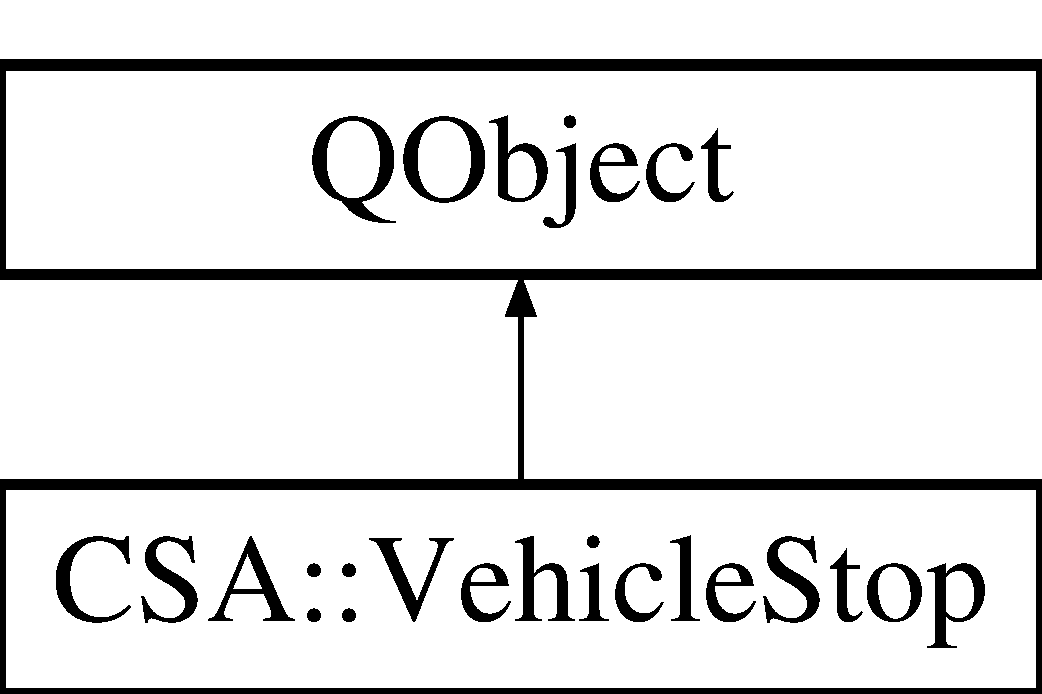
\includegraphics[height=2.000000cm]{classCSA_1_1VehicleStop}
\end{center}
\end{figure}
\subsection*{Public Types}
\begin{DoxyCompactItemize}
\item 
enum \mbox{\hyperlink{classCSA_1_1VehicleStop_a7c2030d5a49808cb8e6fefaa691a76e0}{Type}} \{ \mbox{\hyperlink{classCSA_1_1VehicleStop_a7c2030d5a49808cb8e6fefaa691a76e0ad5f52d91ac49fd146727f4710767dd08}{Type\+::\+A\+R\+R\+I\+V\+AL}}, 
\mbox{\hyperlink{classCSA_1_1VehicleStop_a7c2030d5a49808cb8e6fefaa691a76e0ae7cc381a17e714e7ba15ef6f9858304e}{Type\+::\+D\+E\+P\+A\+R\+T\+U\+RE}}, 
\mbox{\hyperlink{classCSA_1_1VehicleStop_a7c2030d5a49808cb8e6fefaa691a76e0a615a46af313786fc4e349f34118be111}{Type\+::\+S\+T\+OP}}
 \}
\end{DoxyCompactItemize}
\subsection*{Signals}
\begin{DoxyCompactItemize}
\item 
void \mbox{\hyperlink{classCSA_1_1VehicleStop_ae7a43ee3fc70d2359ff12de44b38e6d2}{vehicle\+Information\+Changed}} ()
\item 
void \mbox{\hyperlink{classCSA_1_1VehicleStop_a8cee8183966bb993b1dcc3ca26a483a9}{station\+Changed}} ()
\item 
void \mbox{\hyperlink{classCSA_1_1VehicleStop_a827783ce6df243615d065d5ec49605a6}{platform\+Changed}} ()
\item 
void \mbox{\hyperlink{classCSA_1_1VehicleStop_adbe85cb67383f19a9330160046adf8ab}{is\+Platform\+Normal\+Changed}} ()
\item 
void \mbox{\hyperlink{classCSA_1_1VehicleStop_a009c43f5a3c905a7dcce7b164b75bba4}{has\+Left\+Changed}} ()
\item 
void \mbox{\hyperlink{classCSA_1_1VehicleStop_a0bf965ffe19e1bb16ed3fce5031f56ed}{departure\+Time\+Changed}} ()
\item 
void \mbox{\hyperlink{classCSA_1_1VehicleStop_afba5878d8d99cb87db9d5ce549c2e429}{departure\+Delay\+Changed}} ()
\item 
void \mbox{\hyperlink{classCSA_1_1VehicleStop_a85491b7004511491a9782b6f2bd1155f}{departure\+Canceled\+Changed}} ()
\item 
void \mbox{\hyperlink{classCSA_1_1VehicleStop_ae9f705db514276be05baa892241f797d}{arrival\+Time\+Changed}} ()
\item 
void \mbox{\hyperlink{classCSA_1_1VehicleStop_a371e833cad3ce70195dae5e6917043ee}{arrival\+Delay\+Changed}} ()
\item 
void \mbox{\hyperlink{classCSA_1_1VehicleStop_ad5de2913078d75e0445652cb3e688dc7}{arrival\+Canceled\+Changed}} ()
\item 
void \mbox{\hyperlink{classCSA_1_1VehicleStop_a201e105bb8c1afc2e149c414298c7f52}{departure\+U\+R\+I\+Changed}} ()
\item 
void \mbox{\hyperlink{classCSA_1_1VehicleStop_ae0e96512e3c84393e7d7e641d3163baa}{occupancy\+Level\+Changed}} ()
\item 
void \mbox{\hyperlink{classCSA_1_1VehicleStop_a8a5cffb45c9ea23129662d91fff26385}{type\+Changed}} ()
\end{DoxyCompactItemize}
\subsection*{Public Member Functions}
\begin{DoxyCompactItemize}
\item 
\mbox{\hyperlink{classCSA_1_1VehicleStop_a63f372612a68275d78307b9293339525}{Vehicle\+Stop}} (Q\+Object $\ast$parent=nullptr)
\item 
\mbox{\hyperlink{classCSA_1_1Vehicle}{C\+S\+A\+::\+Vehicle}} $\ast$ \mbox{\hyperlink{classCSA_1_1VehicleStop_ace091d4626e1d5a113f84e9c2b0d07f5}{vehicle\+Information}} () const
\item 
void \mbox{\hyperlink{classCSA_1_1VehicleStop_ac5985077bb7570364bac137c4888c859}{set\+Vehicle\+Information}} (\mbox{\hyperlink{classCSA_1_1Vehicle}{C\+S\+A\+::\+Vehicle}} $\ast$\mbox{\hyperlink{classCSA_1_1VehicleStop_ace091d4626e1d5a113f84e9c2b0d07f5}{vehicle\+Information}})
\item 
\mbox{\hyperlink{classCSA_1_1Station}{C\+S\+A\+::\+Station}} $\ast$ \mbox{\hyperlink{classCSA_1_1VehicleStop_ae1c6e68ec554e65041a2f577433f314d}{station}} () const
\item 
void \mbox{\hyperlink{classCSA_1_1VehicleStop_ae4a990a9e2c462461cf6cdccb129466c}{set\+Station}} (\mbox{\hyperlink{classCSA_1_1Station}{C\+S\+A\+::\+Station}} $\ast$\mbox{\hyperlink{classCSA_1_1VehicleStop_ae1c6e68ec554e65041a2f577433f314d}{station}})
\item 
Q\+String \mbox{\hyperlink{classCSA_1_1VehicleStop_a41eaa371b831197436e9250e5699819a}{platform}} () const
\item 
void \mbox{\hyperlink{classCSA_1_1VehicleStop_a8ef5b90a559539e2a7b46ceed701e06d}{set\+Platform}} (const Q\+String \&\mbox{\hyperlink{classCSA_1_1VehicleStop_a41eaa371b831197436e9250e5699819a}{platform}})
\item 
bool \mbox{\hyperlink{classCSA_1_1VehicleStop_a77b08114a893c3dba935f07496cdb49a}{is\+Platform\+Normal}} () const
\item 
void \mbox{\hyperlink{classCSA_1_1VehicleStop_a55d1d0894b469a1c0018b7a0429a88c0}{set\+Is\+Platform\+Normal}} (bool \mbox{\hyperlink{classCSA_1_1VehicleStop_a77b08114a893c3dba935f07496cdb49a}{is\+Platform\+Normal}})
\item 
bool \mbox{\hyperlink{classCSA_1_1VehicleStop_aeaaf6234293faa5263981162bcc375a7}{has\+Left}} () const
\item 
void \mbox{\hyperlink{classCSA_1_1VehicleStop_ad85c1ed32b7fca5587ec5c64061781a6}{set\+Has\+Left}} (bool \mbox{\hyperlink{classCSA_1_1VehicleStop_aeaaf6234293faa5263981162bcc375a7}{has\+Left}})
\item 
Q\+Date\+Time \mbox{\hyperlink{classCSA_1_1VehicleStop_af7ffcbe1b8db9a40a6cb1c438e6d7a88}{departure\+Time}} () const
\item 
void \mbox{\hyperlink{classCSA_1_1VehicleStop_a29ada511d6218e2421db889a9ef054be}{set\+Departure\+Time}} (const Q\+Date\+Time \&\mbox{\hyperlink{classCSA_1_1VehicleStop_af7ffcbe1b8db9a40a6cb1c438e6d7a88}{departure\+Time}})
\item 
Q\+Date\+Time \mbox{\hyperlink{classCSA_1_1VehicleStop_afc861cba10fcf05779c222fd57f6beeb}{departure\+Delay}} () const
\item 
void \mbox{\hyperlink{classCSA_1_1VehicleStop_aaa5f7c51e5352715fb0e701b3d7560f0}{set\+Departure\+Delay}} (const Q\+Date\+Time \&\mbox{\hyperlink{classCSA_1_1VehicleStop_afc861cba10fcf05779c222fd57f6beeb}{departure\+Delay}})
\item 
Q\+Date\+Time \mbox{\hyperlink{classCSA_1_1VehicleStop_aa02b0117621a7e90a2c38ed10f19a9ee}{departure\+Canceled}} () const
\item 
void \mbox{\hyperlink{classCSA_1_1VehicleStop_afb79c95edf287cd5b40064d1cc94957e}{set\+Departure\+Canceled}} (const Q\+Date\+Time \&\mbox{\hyperlink{classCSA_1_1VehicleStop_aa02b0117621a7e90a2c38ed10f19a9ee}{departure\+Canceled}})
\item 
Q\+Date\+Time \mbox{\hyperlink{classCSA_1_1VehicleStop_af28bb79013b8a29ffedfdd0cc0c96ec7}{arrival\+Time}} () const
\item 
void \mbox{\hyperlink{classCSA_1_1VehicleStop_a96a162d068673f455660531ad549400e}{set\+Arrival\+Time}} (const Q\+Date\+Time \&\mbox{\hyperlink{classCSA_1_1VehicleStop_af28bb79013b8a29ffedfdd0cc0c96ec7}{arrival\+Time}})
\item 
Q\+Date\+Time \mbox{\hyperlink{classCSA_1_1VehicleStop_aa60b346aae368af817fdc0e5d6e3fe30}{arrival\+Delay}} () const
\item 
void \mbox{\hyperlink{classCSA_1_1VehicleStop_ada38acdf633877ba25fa3ada9961c0f6}{set\+Arrival\+Delay}} (const Q\+Date\+Time \&\mbox{\hyperlink{classCSA_1_1VehicleStop_aa60b346aae368af817fdc0e5d6e3fe30}{arrival\+Delay}})
\item 
Q\+Date\+Time \mbox{\hyperlink{classCSA_1_1VehicleStop_a62b0692553adc574939b90a64e91858d}{arrival\+Canceled}} () const
\item 
void \mbox{\hyperlink{classCSA_1_1VehicleStop_a2e5b2e1f111d09a7be6acd933604cd51}{set\+Arrival\+Canceled}} (const Q\+Date\+Time \&\mbox{\hyperlink{classCSA_1_1VehicleStop_a62b0692553adc574939b90a64e91858d}{arrival\+Canceled}})
\item 
Q\+Url \mbox{\hyperlink{classCSA_1_1VehicleStop_a936f754a9b2fd03fd6f4772947f20678}{departure\+U\+RI}} () const
\item 
void \mbox{\hyperlink{classCSA_1_1VehicleStop_afcf73c63b48ba26d8c8df85ca6056177}{set\+Departure\+U\+RI}} (const Q\+Url \&\mbox{\hyperlink{classCSA_1_1VehicleStop_a936f754a9b2fd03fd6f4772947f20678}{departure\+U\+RI}})
\item 
\mbox{\hyperlink{classCSA_1_1Vehicle_a331cc81107e5f0a8f37f894729dd9bda}{C\+S\+A\+::\+Vehicle\+::\+Occupancy\+Level}} \mbox{\hyperlink{classCSA_1_1VehicleStop_a2b1ae10dc6c7b77e5c28ebf646dab03c}{occupancy\+Level}} () const
\item 
void \mbox{\hyperlink{classCSA_1_1VehicleStop_ad23be128248c8d41b64dd60d66877204}{set\+Occupancy\+Level}} (const \mbox{\hyperlink{classCSA_1_1Vehicle_a331cc81107e5f0a8f37f894729dd9bda}{C\+S\+A\+::\+Vehicle\+::\+Occupancy\+Level}} \&\mbox{\hyperlink{classCSA_1_1VehicleStop_a2b1ae10dc6c7b77e5c28ebf646dab03c}{occupancy\+Level}})
\item 
\mbox{\hyperlink{classCSA_1_1VehicleStop_a7c2030d5a49808cb8e6fefaa691a76e0}{C\+S\+A\+::\+Vehicle\+Stop\+::\+Type}} \mbox{\hyperlink{classCSA_1_1VehicleStop_ae104457c93d6b341b140d730cead4bc6}{type}} () const
\item 
void \mbox{\hyperlink{classCSA_1_1VehicleStop_a90bc20355abad4463180a923b3bc3055}{set\+Type}} (const \mbox{\hyperlink{classCSA_1_1VehicleStop_a7c2030d5a49808cb8e6fefaa691a76e0}{C\+S\+A\+::\+Vehicle\+Stop\+::\+Type}} \&\mbox{\hyperlink{classCSA_1_1VehicleStop_ae104457c93d6b341b140d730cead4bc6}{type}})
\end{DoxyCompactItemize}
\subsection*{Private Attributes}
\begin{DoxyCompactItemize}
\item 
\mbox{\hyperlink{classCSA_1_1Vehicle}{C\+S\+A\+::\+Vehicle}} $\ast$ \mbox{\hyperlink{classCSA_1_1VehicleStop_adb8e903136887bad1106057bea070849}{m\+\_\+vehicle\+Information}}
\item 
\mbox{\hyperlink{classCSA_1_1Station}{C\+S\+A\+::\+Station}} $\ast$ \mbox{\hyperlink{classCSA_1_1VehicleStop_a9c9d4bf0d0afb8d354cf1a462018848a}{m\+\_\+station}}
\item 
Q\+String \mbox{\hyperlink{classCSA_1_1VehicleStop_ab8838a2e66e088cb22697429f42fb095}{m\+\_\+platform}}
\item 
bool \mbox{\hyperlink{classCSA_1_1VehicleStop_a80917f349cb1f69d6b45bec5a3ed1348}{m\+\_\+is\+Platform\+Normal}}
\item 
bool \mbox{\hyperlink{classCSA_1_1VehicleStop_a1ad41c255976580494bdd14e86455bdd}{m\+\_\+has\+Left}}
\item 
Q\+Date\+Time \mbox{\hyperlink{classCSA_1_1VehicleStop_a9454125f6563f6a2141850472f33d546}{m\+\_\+departure\+Time}}
\item 
Q\+Date\+Time \mbox{\hyperlink{classCSA_1_1VehicleStop_accc9b62415d4bbf78cb6516c5eb69547}{m\+\_\+departure\+Delay}}
\item 
Q\+Date\+Time \mbox{\hyperlink{classCSA_1_1VehicleStop_a978fcad0cb055cf1ab030cb44d2cf582}{m\+\_\+departure\+Canceled}}
\item 
Q\+Date\+Time \mbox{\hyperlink{classCSA_1_1VehicleStop_a97c5db58b20c001c2eca1d0360339230}{m\+\_\+arrival\+Time}}
\item 
Q\+Date\+Time \mbox{\hyperlink{classCSA_1_1VehicleStop_a5d372323cdccfdb7fc124f1804afe6d6}{m\+\_\+arrival\+Delay}}
\item 
Q\+Date\+Time \mbox{\hyperlink{classCSA_1_1VehicleStop_a38c286c3c0be82c46956589774ee218f}{m\+\_\+arrival\+Canceled}}
\item 
Q\+Url \mbox{\hyperlink{classCSA_1_1VehicleStop_aec621f0a6ce68e2fa31ddf359e416771}{m\+\_\+departure\+U\+RI}}
\item 
\mbox{\hyperlink{classCSA_1_1Vehicle_a331cc81107e5f0a8f37f894729dd9bda}{C\+S\+A\+::\+Vehicle\+::\+Occupancy\+Level}} \mbox{\hyperlink{classCSA_1_1VehicleStop_acb0674aa6848c6e7b183d9c516210cbb}{m\+\_\+occupancy\+Level}}
\item 
\mbox{\hyperlink{classCSA_1_1VehicleStop_a7c2030d5a49808cb8e6fefaa691a76e0}{C\+S\+A\+::\+Vehicle\+Stop\+::\+Type}} \mbox{\hyperlink{classCSA_1_1VehicleStop_a3a162e84b6ca51f7296d65f542e53f44}{m\+\_\+type}}
\end{DoxyCompactItemize}


\subsection{Member Enumeration Documentation}
\mbox{\Hypertarget{classCSA_1_1VehicleStop_a7c2030d5a49808cb8e6fefaa691a76e0}\label{classCSA_1_1VehicleStop_a7c2030d5a49808cb8e6fefaa691a76e0}} 
\index{C\+S\+A\+::\+Vehicle\+Stop@{C\+S\+A\+::\+Vehicle\+Stop}!Type@{Type}}
\index{Type@{Type}!C\+S\+A\+::\+Vehicle\+Stop@{C\+S\+A\+::\+Vehicle\+Stop}}
\subsubsection{\texorpdfstring{Type}{Type}}
{\footnotesize\ttfamily enum \mbox{\hyperlink{classCSA_1_1VehicleStop_a7c2030d5a49808cb8e6fefaa691a76e0}{C\+S\+A\+::\+Vehicle\+Stop\+::\+Type}}\hspace{0.3cm}{\ttfamily [strong]}}

\begin{DoxyEnumFields}{Enumerator}
\raisebox{\heightof{T}}[0pt][0pt]{\index{A\+R\+R\+I\+V\+AL@{A\+R\+R\+I\+V\+AL}!C\+S\+A\+::\+Vehicle\+Stop@{C\+S\+A\+::\+Vehicle\+Stop}}\index{C\+S\+A\+::\+Vehicle\+Stop@{C\+S\+A\+::\+Vehicle\+Stop}!A\+R\+R\+I\+V\+AL@{A\+R\+R\+I\+V\+AL}}}\mbox{\Hypertarget{classCSA_1_1VehicleStop_a7c2030d5a49808cb8e6fefaa691a76e0ad5f52d91ac49fd146727f4710767dd08}\label{classCSA_1_1VehicleStop_a7c2030d5a49808cb8e6fefaa691a76e0ad5f52d91ac49fd146727f4710767dd08}} 
A\+R\+R\+I\+V\+AL&\\
\hline

\raisebox{\heightof{T}}[0pt][0pt]{\index{D\+E\+P\+A\+R\+T\+U\+RE@{D\+E\+P\+A\+R\+T\+U\+RE}!C\+S\+A\+::\+Vehicle\+Stop@{C\+S\+A\+::\+Vehicle\+Stop}}\index{C\+S\+A\+::\+Vehicle\+Stop@{C\+S\+A\+::\+Vehicle\+Stop}!D\+E\+P\+A\+R\+T\+U\+RE@{D\+E\+P\+A\+R\+T\+U\+RE}}}\mbox{\Hypertarget{classCSA_1_1VehicleStop_a7c2030d5a49808cb8e6fefaa691a76e0ae7cc381a17e714e7ba15ef6f9858304e}\label{classCSA_1_1VehicleStop_a7c2030d5a49808cb8e6fefaa691a76e0ae7cc381a17e714e7ba15ef6f9858304e}} 
D\+E\+P\+A\+R\+T\+U\+RE&\\
\hline

\raisebox{\heightof{T}}[0pt][0pt]{\index{S\+T\+OP@{S\+T\+OP}!C\+S\+A\+::\+Vehicle\+Stop@{C\+S\+A\+::\+Vehicle\+Stop}}\index{C\+S\+A\+::\+Vehicle\+Stop@{C\+S\+A\+::\+Vehicle\+Stop}!S\+T\+OP@{S\+T\+OP}}}\mbox{\Hypertarget{classCSA_1_1VehicleStop_a7c2030d5a49808cb8e6fefaa691a76e0a615a46af313786fc4e349f34118be111}\label{classCSA_1_1VehicleStop_a7c2030d5a49808cb8e6fefaa691a76e0a615a46af313786fc4e349f34118be111}} 
S\+T\+OP&\\
\hline

\end{DoxyEnumFields}


\subsection{Constructor \& Destructor Documentation}
\mbox{\Hypertarget{classCSA_1_1VehicleStop_a63f372612a68275d78307b9293339525}\label{classCSA_1_1VehicleStop_a63f372612a68275d78307b9293339525}} 
\index{C\+S\+A\+::\+Vehicle\+Stop@{C\+S\+A\+::\+Vehicle\+Stop}!Vehicle\+Stop@{Vehicle\+Stop}}
\index{Vehicle\+Stop@{Vehicle\+Stop}!C\+S\+A\+::\+Vehicle\+Stop@{C\+S\+A\+::\+Vehicle\+Stop}}
\subsubsection{\texorpdfstring{Vehicle\+Stop()}{VehicleStop()}}
{\footnotesize\ttfamily C\+S\+A\+::\+Vehicle\+Stop\+::\+Vehicle\+Stop (\begin{DoxyParamCaption}\item[{Q\+Object $\ast$}]{parent = {\ttfamily nullptr} }\end{DoxyParamCaption})\hspace{0.3cm}{\ttfamily [explicit]}}



\subsection{Member Function Documentation}
\mbox{\Hypertarget{classCSA_1_1VehicleStop_a62b0692553adc574939b90a64e91858d}\label{classCSA_1_1VehicleStop_a62b0692553adc574939b90a64e91858d}} 
\index{C\+S\+A\+::\+Vehicle\+Stop@{C\+S\+A\+::\+Vehicle\+Stop}!arrival\+Canceled@{arrival\+Canceled}}
\index{arrival\+Canceled@{arrival\+Canceled}!C\+S\+A\+::\+Vehicle\+Stop@{C\+S\+A\+::\+Vehicle\+Stop}}
\subsubsection{\texorpdfstring{arrival\+Canceled()}{arrivalCanceled()}}
{\footnotesize\ttfamily Q\+Date\+Time C\+S\+A\+::\+Vehicle\+Stop\+::arrival\+Canceled (\begin{DoxyParamCaption}{ }\end{DoxyParamCaption}) const}

\mbox{\Hypertarget{classCSA_1_1VehicleStop_ad5de2913078d75e0445652cb3e688dc7}\label{classCSA_1_1VehicleStop_ad5de2913078d75e0445652cb3e688dc7}} 
\index{C\+S\+A\+::\+Vehicle\+Stop@{C\+S\+A\+::\+Vehicle\+Stop}!arrival\+Canceled\+Changed@{arrival\+Canceled\+Changed}}
\index{arrival\+Canceled\+Changed@{arrival\+Canceled\+Changed}!C\+S\+A\+::\+Vehicle\+Stop@{C\+S\+A\+::\+Vehicle\+Stop}}
\subsubsection{\texorpdfstring{arrival\+Canceled\+Changed}{arrivalCanceledChanged}}
{\footnotesize\ttfamily void C\+S\+A\+::\+Vehicle\+Stop\+::arrival\+Canceled\+Changed (\begin{DoxyParamCaption}{ }\end{DoxyParamCaption})\hspace{0.3cm}{\ttfamily [signal]}}

\mbox{\Hypertarget{classCSA_1_1VehicleStop_aa60b346aae368af817fdc0e5d6e3fe30}\label{classCSA_1_1VehicleStop_aa60b346aae368af817fdc0e5d6e3fe30}} 
\index{C\+S\+A\+::\+Vehicle\+Stop@{C\+S\+A\+::\+Vehicle\+Stop}!arrival\+Delay@{arrival\+Delay}}
\index{arrival\+Delay@{arrival\+Delay}!C\+S\+A\+::\+Vehicle\+Stop@{C\+S\+A\+::\+Vehicle\+Stop}}
\subsubsection{\texorpdfstring{arrival\+Delay()}{arrivalDelay()}}
{\footnotesize\ttfamily Q\+Date\+Time C\+S\+A\+::\+Vehicle\+Stop\+::arrival\+Delay (\begin{DoxyParamCaption}{ }\end{DoxyParamCaption}) const}

\mbox{\Hypertarget{classCSA_1_1VehicleStop_a371e833cad3ce70195dae5e6917043ee}\label{classCSA_1_1VehicleStop_a371e833cad3ce70195dae5e6917043ee}} 
\index{C\+S\+A\+::\+Vehicle\+Stop@{C\+S\+A\+::\+Vehicle\+Stop}!arrival\+Delay\+Changed@{arrival\+Delay\+Changed}}
\index{arrival\+Delay\+Changed@{arrival\+Delay\+Changed}!C\+S\+A\+::\+Vehicle\+Stop@{C\+S\+A\+::\+Vehicle\+Stop}}
\subsubsection{\texorpdfstring{arrival\+Delay\+Changed}{arrivalDelayChanged}}
{\footnotesize\ttfamily void C\+S\+A\+::\+Vehicle\+Stop\+::arrival\+Delay\+Changed (\begin{DoxyParamCaption}{ }\end{DoxyParamCaption})\hspace{0.3cm}{\ttfamily [signal]}}

\mbox{\Hypertarget{classCSA_1_1VehicleStop_af28bb79013b8a29ffedfdd0cc0c96ec7}\label{classCSA_1_1VehicleStop_af28bb79013b8a29ffedfdd0cc0c96ec7}} 
\index{C\+S\+A\+::\+Vehicle\+Stop@{C\+S\+A\+::\+Vehicle\+Stop}!arrival\+Time@{arrival\+Time}}
\index{arrival\+Time@{arrival\+Time}!C\+S\+A\+::\+Vehicle\+Stop@{C\+S\+A\+::\+Vehicle\+Stop}}
\subsubsection{\texorpdfstring{arrival\+Time()}{arrivalTime()}}
{\footnotesize\ttfamily Q\+Date\+Time C\+S\+A\+::\+Vehicle\+Stop\+::arrival\+Time (\begin{DoxyParamCaption}{ }\end{DoxyParamCaption}) const}

\mbox{\Hypertarget{classCSA_1_1VehicleStop_ae9f705db514276be05baa892241f797d}\label{classCSA_1_1VehicleStop_ae9f705db514276be05baa892241f797d}} 
\index{C\+S\+A\+::\+Vehicle\+Stop@{C\+S\+A\+::\+Vehicle\+Stop}!arrival\+Time\+Changed@{arrival\+Time\+Changed}}
\index{arrival\+Time\+Changed@{arrival\+Time\+Changed}!C\+S\+A\+::\+Vehicle\+Stop@{C\+S\+A\+::\+Vehicle\+Stop}}
\subsubsection{\texorpdfstring{arrival\+Time\+Changed}{arrivalTimeChanged}}
{\footnotesize\ttfamily void C\+S\+A\+::\+Vehicle\+Stop\+::arrival\+Time\+Changed (\begin{DoxyParamCaption}{ }\end{DoxyParamCaption})\hspace{0.3cm}{\ttfamily [signal]}}

\mbox{\Hypertarget{classCSA_1_1VehicleStop_aa02b0117621a7e90a2c38ed10f19a9ee}\label{classCSA_1_1VehicleStop_aa02b0117621a7e90a2c38ed10f19a9ee}} 
\index{C\+S\+A\+::\+Vehicle\+Stop@{C\+S\+A\+::\+Vehicle\+Stop}!departure\+Canceled@{departure\+Canceled}}
\index{departure\+Canceled@{departure\+Canceled}!C\+S\+A\+::\+Vehicle\+Stop@{C\+S\+A\+::\+Vehicle\+Stop}}
\subsubsection{\texorpdfstring{departure\+Canceled()}{departureCanceled()}}
{\footnotesize\ttfamily Q\+Date\+Time C\+S\+A\+::\+Vehicle\+Stop\+::departure\+Canceled (\begin{DoxyParamCaption}{ }\end{DoxyParamCaption}) const}

\mbox{\Hypertarget{classCSA_1_1VehicleStop_a85491b7004511491a9782b6f2bd1155f}\label{classCSA_1_1VehicleStop_a85491b7004511491a9782b6f2bd1155f}} 
\index{C\+S\+A\+::\+Vehicle\+Stop@{C\+S\+A\+::\+Vehicle\+Stop}!departure\+Canceled\+Changed@{departure\+Canceled\+Changed}}
\index{departure\+Canceled\+Changed@{departure\+Canceled\+Changed}!C\+S\+A\+::\+Vehicle\+Stop@{C\+S\+A\+::\+Vehicle\+Stop}}
\subsubsection{\texorpdfstring{departure\+Canceled\+Changed}{departureCanceledChanged}}
{\footnotesize\ttfamily void C\+S\+A\+::\+Vehicle\+Stop\+::departure\+Canceled\+Changed (\begin{DoxyParamCaption}{ }\end{DoxyParamCaption})\hspace{0.3cm}{\ttfamily [signal]}}

\mbox{\Hypertarget{classCSA_1_1VehicleStop_afc861cba10fcf05779c222fd57f6beeb}\label{classCSA_1_1VehicleStop_afc861cba10fcf05779c222fd57f6beeb}} 
\index{C\+S\+A\+::\+Vehicle\+Stop@{C\+S\+A\+::\+Vehicle\+Stop}!departure\+Delay@{departure\+Delay}}
\index{departure\+Delay@{departure\+Delay}!C\+S\+A\+::\+Vehicle\+Stop@{C\+S\+A\+::\+Vehicle\+Stop}}
\subsubsection{\texorpdfstring{departure\+Delay()}{departureDelay()}}
{\footnotesize\ttfamily Q\+Date\+Time C\+S\+A\+::\+Vehicle\+Stop\+::departure\+Delay (\begin{DoxyParamCaption}{ }\end{DoxyParamCaption}) const}

\mbox{\Hypertarget{classCSA_1_1VehicleStop_afba5878d8d99cb87db9d5ce549c2e429}\label{classCSA_1_1VehicleStop_afba5878d8d99cb87db9d5ce549c2e429}} 
\index{C\+S\+A\+::\+Vehicle\+Stop@{C\+S\+A\+::\+Vehicle\+Stop}!departure\+Delay\+Changed@{departure\+Delay\+Changed}}
\index{departure\+Delay\+Changed@{departure\+Delay\+Changed}!C\+S\+A\+::\+Vehicle\+Stop@{C\+S\+A\+::\+Vehicle\+Stop}}
\subsubsection{\texorpdfstring{departure\+Delay\+Changed}{departureDelayChanged}}
{\footnotesize\ttfamily void C\+S\+A\+::\+Vehicle\+Stop\+::departure\+Delay\+Changed (\begin{DoxyParamCaption}{ }\end{DoxyParamCaption})\hspace{0.3cm}{\ttfamily [signal]}}

\mbox{\Hypertarget{classCSA_1_1VehicleStop_af7ffcbe1b8db9a40a6cb1c438e6d7a88}\label{classCSA_1_1VehicleStop_af7ffcbe1b8db9a40a6cb1c438e6d7a88}} 
\index{C\+S\+A\+::\+Vehicle\+Stop@{C\+S\+A\+::\+Vehicle\+Stop}!departure\+Time@{departure\+Time}}
\index{departure\+Time@{departure\+Time}!C\+S\+A\+::\+Vehicle\+Stop@{C\+S\+A\+::\+Vehicle\+Stop}}
\subsubsection{\texorpdfstring{departure\+Time()}{departureTime()}}
{\footnotesize\ttfamily Q\+Date\+Time C\+S\+A\+::\+Vehicle\+Stop\+::departure\+Time (\begin{DoxyParamCaption}{ }\end{DoxyParamCaption}) const}

\mbox{\Hypertarget{classCSA_1_1VehicleStop_a0bf965ffe19e1bb16ed3fce5031f56ed}\label{classCSA_1_1VehicleStop_a0bf965ffe19e1bb16ed3fce5031f56ed}} 
\index{C\+S\+A\+::\+Vehicle\+Stop@{C\+S\+A\+::\+Vehicle\+Stop}!departure\+Time\+Changed@{departure\+Time\+Changed}}
\index{departure\+Time\+Changed@{departure\+Time\+Changed}!C\+S\+A\+::\+Vehicle\+Stop@{C\+S\+A\+::\+Vehicle\+Stop}}
\subsubsection{\texorpdfstring{departure\+Time\+Changed}{departureTimeChanged}}
{\footnotesize\ttfamily void C\+S\+A\+::\+Vehicle\+Stop\+::departure\+Time\+Changed (\begin{DoxyParamCaption}{ }\end{DoxyParamCaption})\hspace{0.3cm}{\ttfamily [signal]}}

\mbox{\Hypertarget{classCSA_1_1VehicleStop_a936f754a9b2fd03fd6f4772947f20678}\label{classCSA_1_1VehicleStop_a936f754a9b2fd03fd6f4772947f20678}} 
\index{C\+S\+A\+::\+Vehicle\+Stop@{C\+S\+A\+::\+Vehicle\+Stop}!departure\+U\+RI@{departure\+U\+RI}}
\index{departure\+U\+RI@{departure\+U\+RI}!C\+S\+A\+::\+Vehicle\+Stop@{C\+S\+A\+::\+Vehicle\+Stop}}
\subsubsection{\texorpdfstring{departure\+U\+R\+I()}{departureURI()}}
{\footnotesize\ttfamily Q\+Url C\+S\+A\+::\+Vehicle\+Stop\+::departure\+U\+RI (\begin{DoxyParamCaption}{ }\end{DoxyParamCaption}) const}

\mbox{\Hypertarget{classCSA_1_1VehicleStop_a201e105bb8c1afc2e149c414298c7f52}\label{classCSA_1_1VehicleStop_a201e105bb8c1afc2e149c414298c7f52}} 
\index{C\+S\+A\+::\+Vehicle\+Stop@{C\+S\+A\+::\+Vehicle\+Stop}!departure\+U\+R\+I\+Changed@{departure\+U\+R\+I\+Changed}}
\index{departure\+U\+R\+I\+Changed@{departure\+U\+R\+I\+Changed}!C\+S\+A\+::\+Vehicle\+Stop@{C\+S\+A\+::\+Vehicle\+Stop}}
\subsubsection{\texorpdfstring{departure\+U\+R\+I\+Changed}{departureURIChanged}}
{\footnotesize\ttfamily void C\+S\+A\+::\+Vehicle\+Stop\+::departure\+U\+R\+I\+Changed (\begin{DoxyParamCaption}{ }\end{DoxyParamCaption})\hspace{0.3cm}{\ttfamily [signal]}}

\mbox{\Hypertarget{classCSA_1_1VehicleStop_aeaaf6234293faa5263981162bcc375a7}\label{classCSA_1_1VehicleStop_aeaaf6234293faa5263981162bcc375a7}} 
\index{C\+S\+A\+::\+Vehicle\+Stop@{C\+S\+A\+::\+Vehicle\+Stop}!has\+Left@{has\+Left}}
\index{has\+Left@{has\+Left}!C\+S\+A\+::\+Vehicle\+Stop@{C\+S\+A\+::\+Vehicle\+Stop}}
\subsubsection{\texorpdfstring{has\+Left()}{hasLeft()}}
{\footnotesize\ttfamily bool C\+S\+A\+::\+Vehicle\+Stop\+::has\+Left (\begin{DoxyParamCaption}{ }\end{DoxyParamCaption}) const}

\mbox{\Hypertarget{classCSA_1_1VehicleStop_a009c43f5a3c905a7dcce7b164b75bba4}\label{classCSA_1_1VehicleStop_a009c43f5a3c905a7dcce7b164b75bba4}} 
\index{C\+S\+A\+::\+Vehicle\+Stop@{C\+S\+A\+::\+Vehicle\+Stop}!has\+Left\+Changed@{has\+Left\+Changed}}
\index{has\+Left\+Changed@{has\+Left\+Changed}!C\+S\+A\+::\+Vehicle\+Stop@{C\+S\+A\+::\+Vehicle\+Stop}}
\subsubsection{\texorpdfstring{has\+Left\+Changed}{hasLeftChanged}}
{\footnotesize\ttfamily void C\+S\+A\+::\+Vehicle\+Stop\+::has\+Left\+Changed (\begin{DoxyParamCaption}{ }\end{DoxyParamCaption})\hspace{0.3cm}{\ttfamily [signal]}}

\mbox{\Hypertarget{classCSA_1_1VehicleStop_a77b08114a893c3dba935f07496cdb49a}\label{classCSA_1_1VehicleStop_a77b08114a893c3dba935f07496cdb49a}} 
\index{C\+S\+A\+::\+Vehicle\+Stop@{C\+S\+A\+::\+Vehicle\+Stop}!is\+Platform\+Normal@{is\+Platform\+Normal}}
\index{is\+Platform\+Normal@{is\+Platform\+Normal}!C\+S\+A\+::\+Vehicle\+Stop@{C\+S\+A\+::\+Vehicle\+Stop}}
\subsubsection{\texorpdfstring{is\+Platform\+Normal()}{isPlatformNormal()}}
{\footnotesize\ttfamily bool C\+S\+A\+::\+Vehicle\+Stop\+::is\+Platform\+Normal (\begin{DoxyParamCaption}{ }\end{DoxyParamCaption}) const}

\mbox{\Hypertarget{classCSA_1_1VehicleStop_adbe85cb67383f19a9330160046adf8ab}\label{classCSA_1_1VehicleStop_adbe85cb67383f19a9330160046adf8ab}} 
\index{C\+S\+A\+::\+Vehicle\+Stop@{C\+S\+A\+::\+Vehicle\+Stop}!is\+Platform\+Normal\+Changed@{is\+Platform\+Normal\+Changed}}
\index{is\+Platform\+Normal\+Changed@{is\+Platform\+Normal\+Changed}!C\+S\+A\+::\+Vehicle\+Stop@{C\+S\+A\+::\+Vehicle\+Stop}}
\subsubsection{\texorpdfstring{is\+Platform\+Normal\+Changed}{isPlatformNormalChanged}}
{\footnotesize\ttfamily void C\+S\+A\+::\+Vehicle\+Stop\+::is\+Platform\+Normal\+Changed (\begin{DoxyParamCaption}{ }\end{DoxyParamCaption})\hspace{0.3cm}{\ttfamily [signal]}}

\mbox{\Hypertarget{classCSA_1_1VehicleStop_a2b1ae10dc6c7b77e5c28ebf646dab03c}\label{classCSA_1_1VehicleStop_a2b1ae10dc6c7b77e5c28ebf646dab03c}} 
\index{C\+S\+A\+::\+Vehicle\+Stop@{C\+S\+A\+::\+Vehicle\+Stop}!occupancy\+Level@{occupancy\+Level}}
\index{occupancy\+Level@{occupancy\+Level}!C\+S\+A\+::\+Vehicle\+Stop@{C\+S\+A\+::\+Vehicle\+Stop}}
\subsubsection{\texorpdfstring{occupancy\+Level()}{occupancyLevel()}}
{\footnotesize\ttfamily \mbox{\hyperlink{classCSA_1_1Vehicle_a331cc81107e5f0a8f37f894729dd9bda}{C\+S\+A\+::\+Vehicle\+::\+Occupancy\+Level}} C\+S\+A\+::\+Vehicle\+Stop\+::occupancy\+Level (\begin{DoxyParamCaption}{ }\end{DoxyParamCaption}) const}

\mbox{\Hypertarget{classCSA_1_1VehicleStop_ae0e96512e3c84393e7d7e641d3163baa}\label{classCSA_1_1VehicleStop_ae0e96512e3c84393e7d7e641d3163baa}} 
\index{C\+S\+A\+::\+Vehicle\+Stop@{C\+S\+A\+::\+Vehicle\+Stop}!occupancy\+Level\+Changed@{occupancy\+Level\+Changed}}
\index{occupancy\+Level\+Changed@{occupancy\+Level\+Changed}!C\+S\+A\+::\+Vehicle\+Stop@{C\+S\+A\+::\+Vehicle\+Stop}}
\subsubsection{\texorpdfstring{occupancy\+Level\+Changed}{occupancyLevelChanged}}
{\footnotesize\ttfamily void C\+S\+A\+::\+Vehicle\+Stop\+::occupancy\+Level\+Changed (\begin{DoxyParamCaption}{ }\end{DoxyParamCaption})\hspace{0.3cm}{\ttfamily [signal]}}

\mbox{\Hypertarget{classCSA_1_1VehicleStop_a41eaa371b831197436e9250e5699819a}\label{classCSA_1_1VehicleStop_a41eaa371b831197436e9250e5699819a}} 
\index{C\+S\+A\+::\+Vehicle\+Stop@{C\+S\+A\+::\+Vehicle\+Stop}!platform@{platform}}
\index{platform@{platform}!C\+S\+A\+::\+Vehicle\+Stop@{C\+S\+A\+::\+Vehicle\+Stop}}
\subsubsection{\texorpdfstring{platform()}{platform()}}
{\footnotesize\ttfamily Q\+String C\+S\+A\+::\+Vehicle\+Stop\+::platform (\begin{DoxyParamCaption}{ }\end{DoxyParamCaption}) const}

\mbox{\Hypertarget{classCSA_1_1VehicleStop_a827783ce6df243615d065d5ec49605a6}\label{classCSA_1_1VehicleStop_a827783ce6df243615d065d5ec49605a6}} 
\index{C\+S\+A\+::\+Vehicle\+Stop@{C\+S\+A\+::\+Vehicle\+Stop}!platform\+Changed@{platform\+Changed}}
\index{platform\+Changed@{platform\+Changed}!C\+S\+A\+::\+Vehicle\+Stop@{C\+S\+A\+::\+Vehicle\+Stop}}
\subsubsection{\texorpdfstring{platform\+Changed}{platformChanged}}
{\footnotesize\ttfamily void C\+S\+A\+::\+Vehicle\+Stop\+::platform\+Changed (\begin{DoxyParamCaption}{ }\end{DoxyParamCaption})\hspace{0.3cm}{\ttfamily [signal]}}

\mbox{\Hypertarget{classCSA_1_1VehicleStop_a2e5b2e1f111d09a7be6acd933604cd51}\label{classCSA_1_1VehicleStop_a2e5b2e1f111d09a7be6acd933604cd51}} 
\index{C\+S\+A\+::\+Vehicle\+Stop@{C\+S\+A\+::\+Vehicle\+Stop}!set\+Arrival\+Canceled@{set\+Arrival\+Canceled}}
\index{set\+Arrival\+Canceled@{set\+Arrival\+Canceled}!C\+S\+A\+::\+Vehicle\+Stop@{C\+S\+A\+::\+Vehicle\+Stop}}
\subsubsection{\texorpdfstring{set\+Arrival\+Canceled()}{setArrivalCanceled()}}
{\footnotesize\ttfamily void C\+S\+A\+::\+Vehicle\+Stop\+::set\+Arrival\+Canceled (\begin{DoxyParamCaption}\item[{const Q\+Date\+Time \&}]{arrival\+Canceled }\end{DoxyParamCaption})}

\mbox{\Hypertarget{classCSA_1_1VehicleStop_ada38acdf633877ba25fa3ada9961c0f6}\label{classCSA_1_1VehicleStop_ada38acdf633877ba25fa3ada9961c0f6}} 
\index{C\+S\+A\+::\+Vehicle\+Stop@{C\+S\+A\+::\+Vehicle\+Stop}!set\+Arrival\+Delay@{set\+Arrival\+Delay}}
\index{set\+Arrival\+Delay@{set\+Arrival\+Delay}!C\+S\+A\+::\+Vehicle\+Stop@{C\+S\+A\+::\+Vehicle\+Stop}}
\subsubsection{\texorpdfstring{set\+Arrival\+Delay()}{setArrivalDelay()}}
{\footnotesize\ttfamily void C\+S\+A\+::\+Vehicle\+Stop\+::set\+Arrival\+Delay (\begin{DoxyParamCaption}\item[{const Q\+Date\+Time \&}]{arrival\+Delay }\end{DoxyParamCaption})}

\mbox{\Hypertarget{classCSA_1_1VehicleStop_a96a162d068673f455660531ad549400e}\label{classCSA_1_1VehicleStop_a96a162d068673f455660531ad549400e}} 
\index{C\+S\+A\+::\+Vehicle\+Stop@{C\+S\+A\+::\+Vehicle\+Stop}!set\+Arrival\+Time@{set\+Arrival\+Time}}
\index{set\+Arrival\+Time@{set\+Arrival\+Time}!C\+S\+A\+::\+Vehicle\+Stop@{C\+S\+A\+::\+Vehicle\+Stop}}
\subsubsection{\texorpdfstring{set\+Arrival\+Time()}{setArrivalTime()}}
{\footnotesize\ttfamily void C\+S\+A\+::\+Vehicle\+Stop\+::set\+Arrival\+Time (\begin{DoxyParamCaption}\item[{const Q\+Date\+Time \&}]{arrival\+Time }\end{DoxyParamCaption})}

\mbox{\Hypertarget{classCSA_1_1VehicleStop_afb79c95edf287cd5b40064d1cc94957e}\label{classCSA_1_1VehicleStop_afb79c95edf287cd5b40064d1cc94957e}} 
\index{C\+S\+A\+::\+Vehicle\+Stop@{C\+S\+A\+::\+Vehicle\+Stop}!set\+Departure\+Canceled@{set\+Departure\+Canceled}}
\index{set\+Departure\+Canceled@{set\+Departure\+Canceled}!C\+S\+A\+::\+Vehicle\+Stop@{C\+S\+A\+::\+Vehicle\+Stop}}
\subsubsection{\texorpdfstring{set\+Departure\+Canceled()}{setDepartureCanceled()}}
{\footnotesize\ttfamily void C\+S\+A\+::\+Vehicle\+Stop\+::set\+Departure\+Canceled (\begin{DoxyParamCaption}\item[{const Q\+Date\+Time \&}]{departure\+Canceled }\end{DoxyParamCaption})}

\mbox{\Hypertarget{classCSA_1_1VehicleStop_aaa5f7c51e5352715fb0e701b3d7560f0}\label{classCSA_1_1VehicleStop_aaa5f7c51e5352715fb0e701b3d7560f0}} 
\index{C\+S\+A\+::\+Vehicle\+Stop@{C\+S\+A\+::\+Vehicle\+Stop}!set\+Departure\+Delay@{set\+Departure\+Delay}}
\index{set\+Departure\+Delay@{set\+Departure\+Delay}!C\+S\+A\+::\+Vehicle\+Stop@{C\+S\+A\+::\+Vehicle\+Stop}}
\subsubsection{\texorpdfstring{set\+Departure\+Delay()}{setDepartureDelay()}}
{\footnotesize\ttfamily void C\+S\+A\+::\+Vehicle\+Stop\+::set\+Departure\+Delay (\begin{DoxyParamCaption}\item[{const Q\+Date\+Time \&}]{departure\+Delay }\end{DoxyParamCaption})}

\mbox{\Hypertarget{classCSA_1_1VehicleStop_a29ada511d6218e2421db889a9ef054be}\label{classCSA_1_1VehicleStop_a29ada511d6218e2421db889a9ef054be}} 
\index{C\+S\+A\+::\+Vehicle\+Stop@{C\+S\+A\+::\+Vehicle\+Stop}!set\+Departure\+Time@{set\+Departure\+Time}}
\index{set\+Departure\+Time@{set\+Departure\+Time}!C\+S\+A\+::\+Vehicle\+Stop@{C\+S\+A\+::\+Vehicle\+Stop}}
\subsubsection{\texorpdfstring{set\+Departure\+Time()}{setDepartureTime()}}
{\footnotesize\ttfamily void C\+S\+A\+::\+Vehicle\+Stop\+::set\+Departure\+Time (\begin{DoxyParamCaption}\item[{const Q\+Date\+Time \&}]{departure\+Time }\end{DoxyParamCaption})}

\mbox{\Hypertarget{classCSA_1_1VehicleStop_afcf73c63b48ba26d8c8df85ca6056177}\label{classCSA_1_1VehicleStop_afcf73c63b48ba26d8c8df85ca6056177}} 
\index{C\+S\+A\+::\+Vehicle\+Stop@{C\+S\+A\+::\+Vehicle\+Stop}!set\+Departure\+U\+RI@{set\+Departure\+U\+RI}}
\index{set\+Departure\+U\+RI@{set\+Departure\+U\+RI}!C\+S\+A\+::\+Vehicle\+Stop@{C\+S\+A\+::\+Vehicle\+Stop}}
\subsubsection{\texorpdfstring{set\+Departure\+U\+R\+I()}{setDepartureURI()}}
{\footnotesize\ttfamily void C\+S\+A\+::\+Vehicle\+Stop\+::set\+Departure\+U\+RI (\begin{DoxyParamCaption}\item[{const Q\+Url \&}]{departure\+U\+RI }\end{DoxyParamCaption})}

\mbox{\Hypertarget{classCSA_1_1VehicleStop_ad85c1ed32b7fca5587ec5c64061781a6}\label{classCSA_1_1VehicleStop_ad85c1ed32b7fca5587ec5c64061781a6}} 
\index{C\+S\+A\+::\+Vehicle\+Stop@{C\+S\+A\+::\+Vehicle\+Stop}!set\+Has\+Left@{set\+Has\+Left}}
\index{set\+Has\+Left@{set\+Has\+Left}!C\+S\+A\+::\+Vehicle\+Stop@{C\+S\+A\+::\+Vehicle\+Stop}}
\subsubsection{\texorpdfstring{set\+Has\+Left()}{setHasLeft()}}
{\footnotesize\ttfamily void C\+S\+A\+::\+Vehicle\+Stop\+::set\+Has\+Left (\begin{DoxyParamCaption}\item[{bool}]{has\+Left }\end{DoxyParamCaption})}

\mbox{\Hypertarget{classCSA_1_1VehicleStop_a55d1d0894b469a1c0018b7a0429a88c0}\label{classCSA_1_1VehicleStop_a55d1d0894b469a1c0018b7a0429a88c0}} 
\index{C\+S\+A\+::\+Vehicle\+Stop@{C\+S\+A\+::\+Vehicle\+Stop}!set\+Is\+Platform\+Normal@{set\+Is\+Platform\+Normal}}
\index{set\+Is\+Platform\+Normal@{set\+Is\+Platform\+Normal}!C\+S\+A\+::\+Vehicle\+Stop@{C\+S\+A\+::\+Vehicle\+Stop}}
\subsubsection{\texorpdfstring{set\+Is\+Platform\+Normal()}{setIsPlatformNormal()}}
{\footnotesize\ttfamily void C\+S\+A\+::\+Vehicle\+Stop\+::set\+Is\+Platform\+Normal (\begin{DoxyParamCaption}\item[{bool}]{is\+Platform\+Normal }\end{DoxyParamCaption})}

\mbox{\Hypertarget{classCSA_1_1VehicleStop_ad23be128248c8d41b64dd60d66877204}\label{classCSA_1_1VehicleStop_ad23be128248c8d41b64dd60d66877204}} 
\index{C\+S\+A\+::\+Vehicle\+Stop@{C\+S\+A\+::\+Vehicle\+Stop}!set\+Occupancy\+Level@{set\+Occupancy\+Level}}
\index{set\+Occupancy\+Level@{set\+Occupancy\+Level}!C\+S\+A\+::\+Vehicle\+Stop@{C\+S\+A\+::\+Vehicle\+Stop}}
\subsubsection{\texorpdfstring{set\+Occupancy\+Level()}{setOccupancyLevel()}}
{\footnotesize\ttfamily void C\+S\+A\+::\+Vehicle\+Stop\+::set\+Occupancy\+Level (\begin{DoxyParamCaption}\item[{const \mbox{\hyperlink{classCSA_1_1Vehicle_a331cc81107e5f0a8f37f894729dd9bda}{C\+S\+A\+::\+Vehicle\+::\+Occupancy\+Level}} \&}]{occupancy\+Level }\end{DoxyParamCaption})}

\mbox{\Hypertarget{classCSA_1_1VehicleStop_a8ef5b90a559539e2a7b46ceed701e06d}\label{classCSA_1_1VehicleStop_a8ef5b90a559539e2a7b46ceed701e06d}} 
\index{C\+S\+A\+::\+Vehicle\+Stop@{C\+S\+A\+::\+Vehicle\+Stop}!set\+Platform@{set\+Platform}}
\index{set\+Platform@{set\+Platform}!C\+S\+A\+::\+Vehicle\+Stop@{C\+S\+A\+::\+Vehicle\+Stop}}
\subsubsection{\texorpdfstring{set\+Platform()}{setPlatform()}}
{\footnotesize\ttfamily void C\+S\+A\+::\+Vehicle\+Stop\+::set\+Platform (\begin{DoxyParamCaption}\item[{const Q\+String \&}]{platform }\end{DoxyParamCaption})}

\mbox{\Hypertarget{classCSA_1_1VehicleStop_ae4a990a9e2c462461cf6cdccb129466c}\label{classCSA_1_1VehicleStop_ae4a990a9e2c462461cf6cdccb129466c}} 
\index{C\+S\+A\+::\+Vehicle\+Stop@{C\+S\+A\+::\+Vehicle\+Stop}!set\+Station@{set\+Station}}
\index{set\+Station@{set\+Station}!C\+S\+A\+::\+Vehicle\+Stop@{C\+S\+A\+::\+Vehicle\+Stop}}
\subsubsection{\texorpdfstring{set\+Station()}{setStation()}}
{\footnotesize\ttfamily void C\+S\+A\+::\+Vehicle\+Stop\+::set\+Station (\begin{DoxyParamCaption}\item[{\mbox{\hyperlink{classCSA_1_1Station}{C\+S\+A\+::\+Station}} $\ast$}]{station }\end{DoxyParamCaption})}

\mbox{\Hypertarget{classCSA_1_1VehicleStop_a90bc20355abad4463180a923b3bc3055}\label{classCSA_1_1VehicleStop_a90bc20355abad4463180a923b3bc3055}} 
\index{C\+S\+A\+::\+Vehicle\+Stop@{C\+S\+A\+::\+Vehicle\+Stop}!set\+Type@{set\+Type}}
\index{set\+Type@{set\+Type}!C\+S\+A\+::\+Vehicle\+Stop@{C\+S\+A\+::\+Vehicle\+Stop}}
\subsubsection{\texorpdfstring{set\+Type()}{setType()}}
{\footnotesize\ttfamily void C\+S\+A\+::\+Vehicle\+Stop\+::set\+Type (\begin{DoxyParamCaption}\item[{const \mbox{\hyperlink{classCSA_1_1VehicleStop_a7c2030d5a49808cb8e6fefaa691a76e0}{C\+S\+A\+::\+Vehicle\+Stop\+::\+Type}} \&}]{type }\end{DoxyParamCaption})}

\mbox{\Hypertarget{classCSA_1_1VehicleStop_ac5985077bb7570364bac137c4888c859}\label{classCSA_1_1VehicleStop_ac5985077bb7570364bac137c4888c859}} 
\index{C\+S\+A\+::\+Vehicle\+Stop@{C\+S\+A\+::\+Vehicle\+Stop}!set\+Vehicle\+Information@{set\+Vehicle\+Information}}
\index{set\+Vehicle\+Information@{set\+Vehicle\+Information}!C\+S\+A\+::\+Vehicle\+Stop@{C\+S\+A\+::\+Vehicle\+Stop}}
\subsubsection{\texorpdfstring{set\+Vehicle\+Information()}{setVehicleInformation()}}
{\footnotesize\ttfamily void C\+S\+A\+::\+Vehicle\+Stop\+::set\+Vehicle\+Information (\begin{DoxyParamCaption}\item[{\mbox{\hyperlink{classCSA_1_1Vehicle}{C\+S\+A\+::\+Vehicle}} $\ast$}]{vehicle\+Information }\end{DoxyParamCaption})}

\mbox{\Hypertarget{classCSA_1_1VehicleStop_ae1c6e68ec554e65041a2f577433f314d}\label{classCSA_1_1VehicleStop_ae1c6e68ec554e65041a2f577433f314d}} 
\index{C\+S\+A\+::\+Vehicle\+Stop@{C\+S\+A\+::\+Vehicle\+Stop}!station@{station}}
\index{station@{station}!C\+S\+A\+::\+Vehicle\+Stop@{C\+S\+A\+::\+Vehicle\+Stop}}
\subsubsection{\texorpdfstring{station()}{station()}}
{\footnotesize\ttfamily \mbox{\hyperlink{classCSA_1_1Station}{C\+S\+A\+::\+Station}} $\ast$ C\+S\+A\+::\+Vehicle\+Stop\+::station (\begin{DoxyParamCaption}{ }\end{DoxyParamCaption}) const}

\mbox{\Hypertarget{classCSA_1_1VehicleStop_a8cee8183966bb993b1dcc3ca26a483a9}\label{classCSA_1_1VehicleStop_a8cee8183966bb993b1dcc3ca26a483a9}} 
\index{C\+S\+A\+::\+Vehicle\+Stop@{C\+S\+A\+::\+Vehicle\+Stop}!station\+Changed@{station\+Changed}}
\index{station\+Changed@{station\+Changed}!C\+S\+A\+::\+Vehicle\+Stop@{C\+S\+A\+::\+Vehicle\+Stop}}
\subsubsection{\texorpdfstring{station\+Changed}{stationChanged}}
{\footnotesize\ttfamily void C\+S\+A\+::\+Vehicle\+Stop\+::station\+Changed (\begin{DoxyParamCaption}{ }\end{DoxyParamCaption})\hspace{0.3cm}{\ttfamily [signal]}}

\mbox{\Hypertarget{classCSA_1_1VehicleStop_ae104457c93d6b341b140d730cead4bc6}\label{classCSA_1_1VehicleStop_ae104457c93d6b341b140d730cead4bc6}} 
\index{C\+S\+A\+::\+Vehicle\+Stop@{C\+S\+A\+::\+Vehicle\+Stop}!type@{type}}
\index{type@{type}!C\+S\+A\+::\+Vehicle\+Stop@{C\+S\+A\+::\+Vehicle\+Stop}}
\subsubsection{\texorpdfstring{type()}{type()}}
{\footnotesize\ttfamily \mbox{\hyperlink{classCSA_1_1VehicleStop_a7c2030d5a49808cb8e6fefaa691a76e0}{C\+S\+A\+::\+Vehicle\+Stop\+::\+Type}} C\+S\+A\+::\+Vehicle\+Stop\+::type (\begin{DoxyParamCaption}{ }\end{DoxyParamCaption}) const}

\mbox{\Hypertarget{classCSA_1_1VehicleStop_a8a5cffb45c9ea23129662d91fff26385}\label{classCSA_1_1VehicleStop_a8a5cffb45c9ea23129662d91fff26385}} 
\index{C\+S\+A\+::\+Vehicle\+Stop@{C\+S\+A\+::\+Vehicle\+Stop}!type\+Changed@{type\+Changed}}
\index{type\+Changed@{type\+Changed}!C\+S\+A\+::\+Vehicle\+Stop@{C\+S\+A\+::\+Vehicle\+Stop}}
\subsubsection{\texorpdfstring{type\+Changed}{typeChanged}}
{\footnotesize\ttfamily void C\+S\+A\+::\+Vehicle\+Stop\+::type\+Changed (\begin{DoxyParamCaption}{ }\end{DoxyParamCaption})\hspace{0.3cm}{\ttfamily [signal]}}

\mbox{\Hypertarget{classCSA_1_1VehicleStop_ace091d4626e1d5a113f84e9c2b0d07f5}\label{classCSA_1_1VehicleStop_ace091d4626e1d5a113f84e9c2b0d07f5}} 
\index{C\+S\+A\+::\+Vehicle\+Stop@{C\+S\+A\+::\+Vehicle\+Stop}!vehicle\+Information@{vehicle\+Information}}
\index{vehicle\+Information@{vehicle\+Information}!C\+S\+A\+::\+Vehicle\+Stop@{C\+S\+A\+::\+Vehicle\+Stop}}
\subsubsection{\texorpdfstring{vehicle\+Information()}{vehicleInformation()}}
{\footnotesize\ttfamily \mbox{\hyperlink{classCSA_1_1Vehicle}{C\+S\+A\+::\+Vehicle}} $\ast$ C\+S\+A\+::\+Vehicle\+Stop\+::vehicle\+Information (\begin{DoxyParamCaption}{ }\end{DoxyParamCaption}) const}

\mbox{\Hypertarget{classCSA_1_1VehicleStop_ae7a43ee3fc70d2359ff12de44b38e6d2}\label{classCSA_1_1VehicleStop_ae7a43ee3fc70d2359ff12de44b38e6d2}} 
\index{C\+S\+A\+::\+Vehicle\+Stop@{C\+S\+A\+::\+Vehicle\+Stop}!vehicle\+Information\+Changed@{vehicle\+Information\+Changed}}
\index{vehicle\+Information\+Changed@{vehicle\+Information\+Changed}!C\+S\+A\+::\+Vehicle\+Stop@{C\+S\+A\+::\+Vehicle\+Stop}}
\subsubsection{\texorpdfstring{vehicle\+Information\+Changed}{vehicleInformationChanged}}
{\footnotesize\ttfamily void C\+S\+A\+::\+Vehicle\+Stop\+::vehicle\+Information\+Changed (\begin{DoxyParamCaption}{ }\end{DoxyParamCaption})\hspace{0.3cm}{\ttfamily [signal]}}



\subsection{Member Data Documentation}
\mbox{\Hypertarget{classCSA_1_1VehicleStop_a38c286c3c0be82c46956589774ee218f}\label{classCSA_1_1VehicleStop_a38c286c3c0be82c46956589774ee218f}} 
\index{C\+S\+A\+::\+Vehicle\+Stop@{C\+S\+A\+::\+Vehicle\+Stop}!m\+\_\+arrival\+Canceled@{m\+\_\+arrival\+Canceled}}
\index{m\+\_\+arrival\+Canceled@{m\+\_\+arrival\+Canceled}!C\+S\+A\+::\+Vehicle\+Stop@{C\+S\+A\+::\+Vehicle\+Stop}}
\subsubsection{\texorpdfstring{m\+\_\+arrival\+Canceled}{m\_arrivalCanceled}}
{\footnotesize\ttfamily Q\+Date\+Time C\+S\+A\+::\+Vehicle\+Stop\+::m\+\_\+arrival\+Canceled\hspace{0.3cm}{\ttfamily [private]}}

\mbox{\Hypertarget{classCSA_1_1VehicleStop_a5d372323cdccfdb7fc124f1804afe6d6}\label{classCSA_1_1VehicleStop_a5d372323cdccfdb7fc124f1804afe6d6}} 
\index{C\+S\+A\+::\+Vehicle\+Stop@{C\+S\+A\+::\+Vehicle\+Stop}!m\+\_\+arrival\+Delay@{m\+\_\+arrival\+Delay}}
\index{m\+\_\+arrival\+Delay@{m\+\_\+arrival\+Delay}!C\+S\+A\+::\+Vehicle\+Stop@{C\+S\+A\+::\+Vehicle\+Stop}}
\subsubsection{\texorpdfstring{m\+\_\+arrival\+Delay}{m\_arrivalDelay}}
{\footnotesize\ttfamily Q\+Date\+Time C\+S\+A\+::\+Vehicle\+Stop\+::m\+\_\+arrival\+Delay\hspace{0.3cm}{\ttfamily [private]}}

\mbox{\Hypertarget{classCSA_1_1VehicleStop_a97c5db58b20c001c2eca1d0360339230}\label{classCSA_1_1VehicleStop_a97c5db58b20c001c2eca1d0360339230}} 
\index{C\+S\+A\+::\+Vehicle\+Stop@{C\+S\+A\+::\+Vehicle\+Stop}!m\+\_\+arrival\+Time@{m\+\_\+arrival\+Time}}
\index{m\+\_\+arrival\+Time@{m\+\_\+arrival\+Time}!C\+S\+A\+::\+Vehicle\+Stop@{C\+S\+A\+::\+Vehicle\+Stop}}
\subsubsection{\texorpdfstring{m\+\_\+arrival\+Time}{m\_arrivalTime}}
{\footnotesize\ttfamily Q\+Date\+Time C\+S\+A\+::\+Vehicle\+Stop\+::m\+\_\+arrival\+Time\hspace{0.3cm}{\ttfamily [private]}}

\mbox{\Hypertarget{classCSA_1_1VehicleStop_a978fcad0cb055cf1ab030cb44d2cf582}\label{classCSA_1_1VehicleStop_a978fcad0cb055cf1ab030cb44d2cf582}} 
\index{C\+S\+A\+::\+Vehicle\+Stop@{C\+S\+A\+::\+Vehicle\+Stop}!m\+\_\+departure\+Canceled@{m\+\_\+departure\+Canceled}}
\index{m\+\_\+departure\+Canceled@{m\+\_\+departure\+Canceled}!C\+S\+A\+::\+Vehicle\+Stop@{C\+S\+A\+::\+Vehicle\+Stop}}
\subsubsection{\texorpdfstring{m\+\_\+departure\+Canceled}{m\_departureCanceled}}
{\footnotesize\ttfamily Q\+Date\+Time C\+S\+A\+::\+Vehicle\+Stop\+::m\+\_\+departure\+Canceled\hspace{0.3cm}{\ttfamily [private]}}

\mbox{\Hypertarget{classCSA_1_1VehicleStop_accc9b62415d4bbf78cb6516c5eb69547}\label{classCSA_1_1VehicleStop_accc9b62415d4bbf78cb6516c5eb69547}} 
\index{C\+S\+A\+::\+Vehicle\+Stop@{C\+S\+A\+::\+Vehicle\+Stop}!m\+\_\+departure\+Delay@{m\+\_\+departure\+Delay}}
\index{m\+\_\+departure\+Delay@{m\+\_\+departure\+Delay}!C\+S\+A\+::\+Vehicle\+Stop@{C\+S\+A\+::\+Vehicle\+Stop}}
\subsubsection{\texorpdfstring{m\+\_\+departure\+Delay}{m\_departureDelay}}
{\footnotesize\ttfamily Q\+Date\+Time C\+S\+A\+::\+Vehicle\+Stop\+::m\+\_\+departure\+Delay\hspace{0.3cm}{\ttfamily [private]}}

\mbox{\Hypertarget{classCSA_1_1VehicleStop_a9454125f6563f6a2141850472f33d546}\label{classCSA_1_1VehicleStop_a9454125f6563f6a2141850472f33d546}} 
\index{C\+S\+A\+::\+Vehicle\+Stop@{C\+S\+A\+::\+Vehicle\+Stop}!m\+\_\+departure\+Time@{m\+\_\+departure\+Time}}
\index{m\+\_\+departure\+Time@{m\+\_\+departure\+Time}!C\+S\+A\+::\+Vehicle\+Stop@{C\+S\+A\+::\+Vehicle\+Stop}}
\subsubsection{\texorpdfstring{m\+\_\+departure\+Time}{m\_departureTime}}
{\footnotesize\ttfamily Q\+Date\+Time C\+S\+A\+::\+Vehicle\+Stop\+::m\+\_\+departure\+Time\hspace{0.3cm}{\ttfamily [private]}}

\mbox{\Hypertarget{classCSA_1_1VehicleStop_aec621f0a6ce68e2fa31ddf359e416771}\label{classCSA_1_1VehicleStop_aec621f0a6ce68e2fa31ddf359e416771}} 
\index{C\+S\+A\+::\+Vehicle\+Stop@{C\+S\+A\+::\+Vehicle\+Stop}!m\+\_\+departure\+U\+RI@{m\+\_\+departure\+U\+RI}}
\index{m\+\_\+departure\+U\+RI@{m\+\_\+departure\+U\+RI}!C\+S\+A\+::\+Vehicle\+Stop@{C\+S\+A\+::\+Vehicle\+Stop}}
\subsubsection{\texorpdfstring{m\+\_\+departure\+U\+RI}{m\_departureURI}}
{\footnotesize\ttfamily Q\+Url C\+S\+A\+::\+Vehicle\+Stop\+::m\+\_\+departure\+U\+RI\hspace{0.3cm}{\ttfamily [private]}}

\mbox{\Hypertarget{classCSA_1_1VehicleStop_a1ad41c255976580494bdd14e86455bdd}\label{classCSA_1_1VehicleStop_a1ad41c255976580494bdd14e86455bdd}} 
\index{C\+S\+A\+::\+Vehicle\+Stop@{C\+S\+A\+::\+Vehicle\+Stop}!m\+\_\+has\+Left@{m\+\_\+has\+Left}}
\index{m\+\_\+has\+Left@{m\+\_\+has\+Left}!C\+S\+A\+::\+Vehicle\+Stop@{C\+S\+A\+::\+Vehicle\+Stop}}
\subsubsection{\texorpdfstring{m\+\_\+has\+Left}{m\_hasLeft}}
{\footnotesize\ttfamily bool C\+S\+A\+::\+Vehicle\+Stop\+::m\+\_\+has\+Left\hspace{0.3cm}{\ttfamily [private]}}

\mbox{\Hypertarget{classCSA_1_1VehicleStop_a80917f349cb1f69d6b45bec5a3ed1348}\label{classCSA_1_1VehicleStop_a80917f349cb1f69d6b45bec5a3ed1348}} 
\index{C\+S\+A\+::\+Vehicle\+Stop@{C\+S\+A\+::\+Vehicle\+Stop}!m\+\_\+is\+Platform\+Normal@{m\+\_\+is\+Platform\+Normal}}
\index{m\+\_\+is\+Platform\+Normal@{m\+\_\+is\+Platform\+Normal}!C\+S\+A\+::\+Vehicle\+Stop@{C\+S\+A\+::\+Vehicle\+Stop}}
\subsubsection{\texorpdfstring{m\+\_\+is\+Platform\+Normal}{m\_isPlatformNormal}}
{\footnotesize\ttfamily bool C\+S\+A\+::\+Vehicle\+Stop\+::m\+\_\+is\+Platform\+Normal\hspace{0.3cm}{\ttfamily [private]}}

\mbox{\Hypertarget{classCSA_1_1VehicleStop_acb0674aa6848c6e7b183d9c516210cbb}\label{classCSA_1_1VehicleStop_acb0674aa6848c6e7b183d9c516210cbb}} 
\index{C\+S\+A\+::\+Vehicle\+Stop@{C\+S\+A\+::\+Vehicle\+Stop}!m\+\_\+occupancy\+Level@{m\+\_\+occupancy\+Level}}
\index{m\+\_\+occupancy\+Level@{m\+\_\+occupancy\+Level}!C\+S\+A\+::\+Vehicle\+Stop@{C\+S\+A\+::\+Vehicle\+Stop}}
\subsubsection{\texorpdfstring{m\+\_\+occupancy\+Level}{m\_occupancyLevel}}
{\footnotesize\ttfamily \mbox{\hyperlink{classCSA_1_1Vehicle_a331cc81107e5f0a8f37f894729dd9bda}{C\+S\+A\+::\+Vehicle\+::\+Occupancy\+Level}} C\+S\+A\+::\+Vehicle\+Stop\+::m\+\_\+occupancy\+Level\hspace{0.3cm}{\ttfamily [private]}}

\mbox{\Hypertarget{classCSA_1_1VehicleStop_ab8838a2e66e088cb22697429f42fb095}\label{classCSA_1_1VehicleStop_ab8838a2e66e088cb22697429f42fb095}} 
\index{C\+S\+A\+::\+Vehicle\+Stop@{C\+S\+A\+::\+Vehicle\+Stop}!m\+\_\+platform@{m\+\_\+platform}}
\index{m\+\_\+platform@{m\+\_\+platform}!C\+S\+A\+::\+Vehicle\+Stop@{C\+S\+A\+::\+Vehicle\+Stop}}
\subsubsection{\texorpdfstring{m\+\_\+platform}{m\_platform}}
{\footnotesize\ttfamily Q\+String C\+S\+A\+::\+Vehicle\+Stop\+::m\+\_\+platform\hspace{0.3cm}{\ttfamily [private]}}

\mbox{\Hypertarget{classCSA_1_1VehicleStop_a9c9d4bf0d0afb8d354cf1a462018848a}\label{classCSA_1_1VehicleStop_a9c9d4bf0d0afb8d354cf1a462018848a}} 
\index{C\+S\+A\+::\+Vehicle\+Stop@{C\+S\+A\+::\+Vehicle\+Stop}!m\+\_\+station@{m\+\_\+station}}
\index{m\+\_\+station@{m\+\_\+station}!C\+S\+A\+::\+Vehicle\+Stop@{C\+S\+A\+::\+Vehicle\+Stop}}
\subsubsection{\texorpdfstring{m\+\_\+station}{m\_station}}
{\footnotesize\ttfamily \mbox{\hyperlink{classCSA_1_1Station}{C\+S\+A\+::\+Station}}$\ast$ C\+S\+A\+::\+Vehicle\+Stop\+::m\+\_\+station\hspace{0.3cm}{\ttfamily [private]}}

\mbox{\Hypertarget{classCSA_1_1VehicleStop_a3a162e84b6ca51f7296d65f542e53f44}\label{classCSA_1_1VehicleStop_a3a162e84b6ca51f7296d65f542e53f44}} 
\index{C\+S\+A\+::\+Vehicle\+Stop@{C\+S\+A\+::\+Vehicle\+Stop}!m\+\_\+type@{m\+\_\+type}}
\index{m\+\_\+type@{m\+\_\+type}!C\+S\+A\+::\+Vehicle\+Stop@{C\+S\+A\+::\+Vehicle\+Stop}}
\subsubsection{\texorpdfstring{m\+\_\+type}{m\_type}}
{\footnotesize\ttfamily \mbox{\hyperlink{classCSA_1_1VehicleStop_a7c2030d5a49808cb8e6fefaa691a76e0}{C\+S\+A\+::\+Vehicle\+Stop\+::\+Type}} C\+S\+A\+::\+Vehicle\+Stop\+::m\+\_\+type\hspace{0.3cm}{\ttfamily [private]}}

\mbox{\Hypertarget{classCSA_1_1VehicleStop_adb8e903136887bad1106057bea070849}\label{classCSA_1_1VehicleStop_adb8e903136887bad1106057bea070849}} 
\index{C\+S\+A\+::\+Vehicle\+Stop@{C\+S\+A\+::\+Vehicle\+Stop}!m\+\_\+vehicle\+Information@{m\+\_\+vehicle\+Information}}
\index{m\+\_\+vehicle\+Information@{m\+\_\+vehicle\+Information}!C\+S\+A\+::\+Vehicle\+Stop@{C\+S\+A\+::\+Vehicle\+Stop}}
\subsubsection{\texorpdfstring{m\+\_\+vehicle\+Information}{m\_vehicleInformation}}
{\footnotesize\ttfamily \mbox{\hyperlink{classCSA_1_1Vehicle}{C\+S\+A\+::\+Vehicle}}$\ast$ C\+S\+A\+::\+Vehicle\+Stop\+::m\+\_\+vehicle\+Information\hspace{0.3cm}{\ttfamily [private]}}



The documentation for this class was generated from the following files\+:\begin{DoxyCompactItemize}
\item 
src/linkedconnections/csa/\mbox{\hyperlink{csavehiclestop_8h}{csavehiclestop.\+h}}\item 
src/linkedconnections/csa/\mbox{\hyperlink{csavehiclestop_8cpp}{csavehiclestop.\+cpp}}\end{DoxyCompactItemize}

\chapter{File Documentation}
\hypertarget{databasemanager_8cpp}{}\section{src/database/databasemanager.cpp File Reference}
\label{databasemanager_8cpp}\index{src/database/databasemanager.\+cpp@{src/database/databasemanager.\+cpp}}


Manager facade constructor.  


{\ttfamily \#include \char`\"{}database/databasemanager.\+h\char`\"{}}\newline
\subsection*{Namespaces}
\begin{DoxyCompactItemize}
\item 
 \mbox{\hyperlink{namespaceDatabase}{Database}}
\end{DoxyCompactItemize}


\subsection{Detailed Description}
Manager facade constructor. 

Gets the current Q\+Sql\+Database database.

Sets the Q\+Sql\+Database database.

Ends the transaction.

Starts the transaction.

Executes a given Q\+Sql\+Query asynchronous.

Executes a given Q\+Sql\+Query.

Gets a \mbox{\hyperlink{classDatabase_1_1Manager}{Database\+::\+Manager}} instance.

\begin{DoxyAuthor}{Author}
Dylan Van Assche 
\end{DoxyAuthor}
\begin{DoxyDate}{Date}
20 Jul 2018 
\end{DoxyDate}

\begin{DoxyParams}{Parameters}
{\em Q\+Object} & $\ast$parent \\
\hline
{\em Q\+String} & path\\
\hline
\end{DoxyParams}
\begin{DoxyAuthor}{Author}
Dylan Van Assche 
\end{DoxyAuthor}
\begin{DoxyDate}{Date}
21 Jul 2018 
\end{DoxyDate}
\begin{DoxyReturn}{Returns}
\mbox{\hyperlink{classDatabase_1_1Manager}{Database\+::\+Manager}} $\ast$manager
\end{DoxyReturn}
\begin{DoxyAuthor}{Author}
Dylan Van Assche 
\end{DoxyAuthor}
\begin{DoxyDate}{Date}
20 Jul 2018 
\end{DoxyDate}

\begin{DoxyParams}{Parameters}
{\em Q\+Sql\+Query} & query \\
\hline
\end{DoxyParams}
\begin{DoxyReturn}{Returns}
bool success
\end{DoxyReturn}
\begin{DoxyAuthor}{Author}
Dylan Van Assche 
\end{DoxyAuthor}
\begin{DoxyDate}{Date}
13 Aug 2018 
\end{DoxyDate}

\begin{DoxyParams}{Parameters}
{\em Q\+Sql\+Query} & query \\
\hline
\end{DoxyParams}
\begin{DoxyReturn}{Returns}
bool success
\end{DoxyReturn}
\begin{DoxyAuthor}{Author}
Dylan Van Assche 
\end{DoxyAuthor}
\begin{DoxyDate}{Date}
9 Aug 2018 
\end{DoxyDate}
\begin{DoxyReturn}{Returns}
bool success
\end{DoxyReturn}
\begin{DoxyAuthor}{Author}
Dylan Van Assche 
\end{DoxyAuthor}
\begin{DoxyDate}{Date}
20 Jul 2018 
\end{DoxyDate}

\begin{DoxyParams}{Parameters}
{\em const} & Q\+Sql\+Database \&database\\
\hline
\end{DoxyParams}
\begin{DoxyAuthor}{Author}
Dylan Van Assche 
\end{DoxyAuthor}
\begin{DoxyDate}{Date}
20 Jul 2018 
\end{DoxyDate}
\begin{DoxyReturn}{Returns}
Q\+Sql\+Database database 
\end{DoxyReturn}

\hypertarget{databasemanager_8h}{}\section{src/include/database/databasemanager.h File Reference}
\label{databasemanager_8h}\index{src/include/database/databasemanager.h@{src/include/database/databasemanager.h}}
{\ttfamily \#include $<$Qt\+Core/\+Qt\+Global$>$}\newline
{\ttfamily \#include $<$Qt\+Core/\+Qt\+Debug$>$}\newline
{\ttfamily \#include $<$Qt\+Core/\+Q\+Object$>$}\newline
{\ttfamily \#include $<$Qt\+Core/\+Q\+String$>$}\newline
{\ttfamily \#include $<$Qt\+Core/\+Q\+Uuid$>$}\newline
{\ttfamily \#include $<$Qt\+Core/\+Q\+Future$>$}\newline
{\ttfamily \#include $<$Qt\+Sql/\+Q\+Sql\+Database$>$}\newline
{\ttfamily \#include $<$Qt\+Sql/\+Q\+Sql\+Driver$>$}\newline
{\ttfamily \#include $<$Qt\+Sql/\+Q\+Sql\+Error$>$}\newline
{\ttfamily \#include $<$Qt\+Sql/\+Q\+Sql\+Query$>$}\newline
{\ttfamily \#include $<$Qt\+Core/\+Q\+Thread\+Storage$>$}\newline
\subsection*{Data Structures}
\begin{DoxyCompactItemize}
\item 
class \mbox{\hyperlink{classQRail_1_1Database_1_1Manager}{Q\+Rail\+::\+Database\+::\+Manager}}
\begin{DoxyCompactList}\small\item\em The \mbox{\hyperlink{classQRail_1_1Database_1_1Manager}{Database\+::\+Manager}} class manages a given database. \end{DoxyCompactList}\end{DoxyCompactItemize}
\subsection*{Namespaces}
\begin{DoxyCompactItemize}
\item 
 \mbox{\hyperlink{namespaceQRail}{Q\+Rail}}
\item 
 \mbox{\hyperlink{namespaceQRail_1_1Database}{Q\+Rail\+::\+Database}}
\end{DoxyCompactItemize}
\subsection*{Macros}
\begin{DoxyCompactItemize}
\item 
\#define \mbox{\hyperlink{databasemanager_8h_a45044c35ca9fe4a00b497f05d2b818cc}{D\+R\+I\+V\+ER}}~\char`\"{}Q\+S\+Q\+L\+I\+TE\char`\"{}
\end{DoxyCompactItemize}


\subsection{Macro Definition Documentation}
\mbox{\Hypertarget{databasemanager_8h_a45044c35ca9fe4a00b497f05d2b818cc}\label{databasemanager_8h_a45044c35ca9fe4a00b497f05d2b818cc}} 
\index{databasemanager.h@{databasemanager.h}!DRIVER@{DRIVER}}
\index{DRIVER@{DRIVER}!databasemanager.h@{databasemanager.h}}
\subsubsection{\texorpdfstring{DRIVER}{DRIVER}}
{\footnotesize\ttfamily \#define D\+R\+I\+V\+ER~\char`\"{}Q\+S\+Q\+L\+I\+TE\char`\"{}}


\hypertarget{harbour-berail_8cpp}{}\section{src/harbour-\/berail.cpp File Reference}
\label{harbour-berail_8cpp}\index{src/harbour-\/berail.\+cpp@{src/harbour-\/berail.\+cpp}}
{\ttfamily \#include $<$sailfishapp.\+h$>$}\newline
{\ttfamily \#include $<$Qt\+Core/\+Q\+Scoped\+Pointer$>$}\newline
{\ttfamily \#include $<$Qt\+Core/\+Q\+String$>$}\newline
{\ttfamily \#include $<$Qt\+Core/\+Q\+Translator$>$}\newline
{\ttfamily \#include $<$Qt\+Gui/\+Q\+Gui\+Application$>$}\newline
{\ttfamily \#include $<$Qt\+Quick/\+Q\+Quick\+View$>$}\newline
{\ttfamily \#include $<$Qt\+Qml/\+Q\+Qml\+Engine$>$}\newline
{\ttfamily \#include \char`\"{}logger.\+h\char`\"{}}\newline
{\ttfamily \#include \char`\"{}os.\+h\char`\"{}}\newline
{\ttfamily \#include \char`\"{}../tests/network/networkmanagertest.\+h\char`\"{}}\newline
{\ttfamily \#include \char`\"{}../tests/database/databasemanagertest.\+h\char`\"{}}\newline
{\ttfamily \#include \char`\"{}../tests/fragments/fragmentsfragmenttest.\+h\char`\"{}}\newline
{\ttfamily \#include \char`\"{}../tests/fragments/fragmentspagetest.\+h\char`\"{}}\newline
{\ttfamily \#include \char`\"{}../tests/fragments/fragmentsfactorytest.\+h\char`\"{}}\newline
{\ttfamily \#include \char`\"{}../tests/csa/csaplannertest.\+h\char`\"{}}\newline
\subsection*{Functions}
\begin{DoxyCompactItemize}
\item 
int \mbox{\hyperlink{harbour-berail_8cpp_a0ddf1224851353fc92bfbff6f499fa97}{main}} (int argc, char $\ast$argv\mbox{[}$\,$\mbox{]})
\end{DoxyCompactItemize}


\subsection{Function Documentation}
\mbox{\Hypertarget{harbour-berail_8cpp_a0ddf1224851353fc92bfbff6f499fa97}\label{harbour-berail_8cpp_a0ddf1224851353fc92bfbff6f499fa97}} 
\index{harbour-\/berail.\+cpp@{harbour-\/berail.\+cpp}!main@{main}}
\index{main@{main}!harbour-\/berail.\+cpp@{harbour-\/berail.\+cpp}}
\subsubsection{\texorpdfstring{main()}{main()}}
{\footnotesize\ttfamily int main (\begin{DoxyParamCaption}\item[{int}]{argc,  }\item[{char $\ast$}]{argv\mbox{[}$\,$\mbox{]} }\end{DoxyParamCaption})}


\hypertarget{csamessage_8cpp}{}\section{src/linkedconnections/csa/csamessage.cpp File Reference}
\label{csamessage_8cpp}\index{src/linkedconnections/csa/csamessage.\+cpp@{src/linkedconnections/csa/csamessage.\+cpp}}


Message constructor\+: full.  


{\ttfamily \#include \char`\"{}csamessage.\+h\char`\"{}}\newline
\subsection*{Namespaces}
\begin{DoxyCompactItemize}
\item 
 \mbox{\hyperlink{namespaceCSA}{C\+SA}}
\end{DoxyCompactItemize}


\subsection{Detailed Description}
Message constructor\+: full. 

Sets the link.

Gets the link.

Sets the lead.

Gets the lead.

Sets the description.

Gets the description.

Sets the header.

Gets the header.

Message constructor\+: minimum.

\begin{DoxyAuthor}{Author}
Dylan Van Assche 
\end{DoxyAuthor}
\begin{DoxyDate}{Date}
09 Aug 2018 
\end{DoxyDate}

\begin{DoxyParams}{Parameters}
{\em const} & Q\+String \&header \\
\hline
{\em const} & Q\+String \&description \\
\hline
{\em const} & Q\+String \&lead \\
\hline
{\em const} & Q\+Url \&link \\
\hline
{\em Q\+Object} & $\ast$parent\\
\hline
\end{DoxyParams}
\begin{DoxyAuthor}{Author}
Dylan Van Assche 
\end{DoxyAuthor}
\begin{DoxyDate}{Date}
09 Aug 2018 
\end{DoxyDate}

\begin{DoxyParams}{Parameters}
{\em const} & Q\+String \&header \\
\hline
{\em const} & Q\+String \&description \\
\hline
{\em Q\+Object} & $\ast$parent\\
\hline
\end{DoxyParams}
\begin{DoxyAuthor}{Author}
Dylan Van Assche 
\end{DoxyAuthor}
\begin{DoxyDate}{Date}
09 Aug 2018 
\end{DoxyDate}
\begin{DoxyReturn}{Returns}
Q\+String header
\end{DoxyReturn}
\begin{DoxyAuthor}{Author}
Dylan Van Assche 
\end{DoxyAuthor}
\begin{DoxyDate}{Date}
09 Aug 2018 
\end{DoxyDate}

\begin{DoxyParams}{Parameters}
{\em const} & Q\+String \&header\\
\hline
\end{DoxyParams}
\begin{DoxyAuthor}{Author}
Dylan Van Assche 
\end{DoxyAuthor}
\begin{DoxyDate}{Date}
09 Aug 2018 
\end{DoxyDate}
\begin{DoxyReturn}{Returns}
Q\+String description
\end{DoxyReturn}
\begin{DoxyAuthor}{Author}
Dylan Van Assche 
\end{DoxyAuthor}
\begin{DoxyDate}{Date}
09 Aug 2018 
\end{DoxyDate}

\begin{DoxyParams}{Parameters}
{\em const} & Q\+String \&description\\
\hline
\end{DoxyParams}
\begin{DoxyAuthor}{Author}
Dylan Van Assche 
\end{DoxyAuthor}
\begin{DoxyDate}{Date}
09 Aug 2018 
\end{DoxyDate}
\begin{DoxyReturn}{Returns}
Q\+String lead
\end{DoxyReturn}
\begin{DoxyAuthor}{Author}
Dylan Van Assche 
\end{DoxyAuthor}
\begin{DoxyDate}{Date}
09 Aug 2018 
\end{DoxyDate}

\begin{DoxyParams}{Parameters}
{\em const} & Q\+String \&lead\\
\hline
\end{DoxyParams}
\begin{DoxyAuthor}{Author}
Dylan Van Assche 
\end{DoxyAuthor}
\begin{DoxyDate}{Date}
09 Aug 2018 
\end{DoxyDate}
\begin{DoxyReturn}{Returns}
Q\+Url link
\end{DoxyReturn}
\begin{DoxyAuthor}{Author}
Dylan Van Assche 
\end{DoxyAuthor}
\begin{DoxyDate}{Date}
09 Aug 2018 
\end{DoxyDate}

\begin{DoxyParams}{Parameters}
{\em const} & Q\+Url \&link \\
\hline
\end{DoxyParams}

\hypertarget{csamessage_8h}{}\section{src/linkedconnections/csa/csamessage.h File Reference}
\label{csamessage_8h}\index{src/linkedconnections/csa/csamessage.\+h@{src/linkedconnections/csa/csamessage.\+h}}
{\ttfamily \#include $<$Qt\+Core/\+Q\+Object$>$}\newline
{\ttfamily \#include $<$Qt\+Core/\+Q\+String$>$}\newline
{\ttfamily \#include $<$Qt\+Core/\+Q\+Url$>$}\newline
\subsection*{Classes}
\begin{DoxyCompactItemize}
\item 
class \mbox{\hyperlink{classCSA_1_1Message}{C\+S\+A\+::\+Message}}
\end{DoxyCompactItemize}
\subsection*{Namespaces}
\begin{DoxyCompactItemize}
\item 
 \mbox{\hyperlink{namespaceCSA}{C\+SA}}
\end{DoxyCompactItemize}

\hypertarget{csanullstation_8cpp}{}\section{src/linkedconnections/csa/csanullstation.cpp File Reference}
\label{csanullstation_8cpp}\index{src/linkedconnections/csa/csanullstation.\+cpp@{src/linkedconnections/csa/csanullstation.\+cpp}}


\mbox{\hyperlink{classCSA_1_1NullStation}{C\+S\+A\+::\+Null\+Station}} constructor.  


{\ttfamily \#include \char`\"{}csanullstation.\+h\char`\"{}}\newline
\subsection*{Namespaces}
\begin{DoxyCompactItemize}
\item 
 \mbox{\hyperlink{namespaceCSA}{C\+SA}}
\end{DoxyCompactItemize}


\subsection{Detailed Description}
\mbox{\hyperlink{classCSA_1_1NullStation}{C\+S\+A\+::\+Null\+Station}} constructor. 

Gets a \mbox{\hyperlink{classCSA_1_1NullStation}{C\+S\+A\+::\+Null\+Station}} instance.

\begin{DoxyAuthor}{Author}
Dylan Van Assche 
\end{DoxyAuthor}
\begin{DoxyDate}{Date}
09 Aug 2018 
\end{DoxyDate}

\begin{DoxyParams}{Parameters}
{\em const} & Q\+Url \&uri \\
\hline
{\em const} & Q\+Map$<$\+Q\+Locale\+::\+Language, Q\+String$>$ \&name \\
\hline
{\em const} & Q\+Locale\+::\+Country \&country \\
\hline
{\em const} & Q\+Geo\+Coordinate \&position \\
\hline
{\em const} & Q\+Geo\+Address \&address \\
\hline
{\em const} & bool \&has\+Ticket\+Vending\+Machine \\
\hline
{\em const} & bool \&has\+Luggage\+Lockers \\
\hline
{\em const} & bool \&has\+Free\+Parking \\
\hline
{\em const} & bool \&has\+Taxi \\
\hline
{\em const} & bool \&has\+Bicycl\+Spots \\
\hline
{\em const} & bool \&has\+Bus \\
\hline
{\em const} & bool \&has\+Tram \\
\hline
{\em const} & bool \&has\+Metro \\
\hline
{\em const} & bool \&has\+Wheelchair\+Available \\
\hline
{\em const} & bool \&has\+Ramp \\
\hline
{\em const} & qint16 \&disabled\+Parking\+Spots \\
\hline
{\em const} & bool \&has\+Elevated\+Platform \\
\hline
{\em const} & bool \&has\+Escalator\+Up \\
\hline
{\em const} & bool \&has\+Escalator\+Down \\
\hline
{\em const} & bool \&has\+Elevator\+Platform \\
\hline
{\em const} & bool \&has\+Hearing\+Aid\+Signal \\
\hline
{\em const} & Q\+Map$<$\mbox{\hyperlink{classCSA_1_1Station_aa160d0de40db0583099b5986dea1cd67}{C\+S\+A\+::\+Station\+::\+Day}}, Q\+Pair$<$\+Q\+Time, Q\+Time$>$$>$ \&opening\+Hours \\
\hline
{\em const} & qreal \&average\+Stop\+Times \\
\hline
{\em Q\+Object} & $\ast$parent\\
\hline
\end{DoxyParams}
\begin{DoxyAuthor}{Author}
Dylan Van Assche 
\end{DoxyAuthor}
\begin{DoxyDate}{Date}
09 Aug 2018 
\end{DoxyDate}

\begin{DoxyParams}{Parameters}
{\em Q\+Object} & $\ast$parent = nullptr \\
\hline
\end{DoxyParams}
\begin{DoxyReturn}{Returns}
\mbox{\hyperlink{classCSA_1_1NullStation}{C\+S\+A\+::\+Null\+Station}} $\ast$station 
\end{DoxyReturn}

\hypertarget{csanullstation_8h}{}\section{src/linkedconnections/csa/csanullstation.h File Reference}
\label{csanullstation_8h}\index{src/linkedconnections/csa/csanullstation.\+h@{src/linkedconnections/csa/csanullstation.\+h}}
{\ttfamily \#include $<$Qt\+Core/\+Q\+Object$>$}\newline
{\ttfamily \#include $<$Qt\+Core/\+Q\+Debug$>$}\newline
{\ttfamily \#include $<$Qt\+Core/\+Q\+Map$>$}\newline
{\ttfamily \#include $<$Qt\+Core/\+Q\+Locale$>$}\newline
{\ttfamily \#include $<$Qt\+Core/\+Q\+Time$>$}\newline
{\ttfamily \#include $<$Qt\+Core/\+Q\+Pair$>$}\newline
{\ttfamily \#include $<$Qt\+Positioning/\+Q\+Geo\+Address$>$}\newline
{\ttfamily \#include $<$Qt\+Positioning/\+Q\+Geo\+Coordinate$>$}\newline
{\ttfamily \#include \char`\"{}csastation.\+h\char`\"{}}\newline
\subsection*{Classes}
\begin{DoxyCompactItemize}
\item 
class \mbox{\hyperlink{classCSA_1_1NullStation}{C\+S\+A\+::\+Null\+Station}}
\end{DoxyCompactItemize}
\subsection*{Namespaces}
\begin{DoxyCompactItemize}
\item 
 \mbox{\hyperlink{namespaceCSA}{C\+SA}}
\end{DoxyCompactItemize}

\hypertarget{csaplanner_8cpp}{}\section{src/linkedconnections/csa/csaplanner.cpp File Reference}
\label{csaplanner_8cpp}\index{src/linkedconnections/csa/csaplanner.\+cpp@{src/linkedconnections/csa/csaplanner.\+cpp}}
{\ttfamily \#include \char`\"{}csaplanner.\+h\char`\"{}}\newline

\hypertarget{csaplanner_8h}{}\section{src/linkedconnections/csa/csaplanner.h File Reference}
\label{csaplanner_8h}\index{src/linkedconnections/csa/csaplanner.\+h@{src/linkedconnections/csa/csaplanner.\+h}}
{\ttfamily \#include $<$Qt\+Core/\+Qt\+Global$>$}\newline
{\ttfamily \#include $<$Qt\+Core/\+Q\+Object$>$}\newline
{\ttfamily \#include $<$Qt\+Core/\+Q\+Date\+Time$>$}\newline
{\ttfamily \#include $<$Qt\+Core/\+Q\+List$>$}\newline
{\ttfamily \#include $<$Qt\+Core/\+Q\+Locale$>$}\newline
{\ttfamily \#include $<$Qt\+Core/\+Q\+Pair$>$}\newline
{\ttfamily \#include $<$Qt\+Core/\+Q\+Map$>$}\newline
{\ttfamily \#include $<$Qt\+Core/\+Q\+Mutex$>$}\newline
{\ttfamily \#include $<$Qt\+Core/\+Q\+Mutex\+Locker$>$}\newline
{\ttfamily \#include $<$Qt\+Concurrent/\+Qt\+Concurrent$>$}\newline
{\ttfamily \#include $<$algorithm$>$}\newline
{\ttfamily \#include \char`\"{}../fragments/fragmentsfactory.\+h\char`\"{}}\newline
{\ttfamily \#include \char`\"{}csastationstopprofile.\+h\char`\"{}}\newline
{\ttfamily \#include \char`\"{}csatrainprofile.\+h\char`\"{}}\newline
{\ttfamily \#include \char`\"{}csaroute.\+h\char`\"{}}\newline
{\ttfamily \#include \char`\"{}csarouteleg.\+h\char`\"{}}\newline
{\ttfamily \#include \char`\"{}csaroutelegend.\+h\char`\"{}}\newline
{\ttfamily \#include \char`\"{}csatransfer.\+h\char`\"{}}\newline
{\ttfamily \#include \char`\"{}csamessage.\+h\char`\"{}}\newline
{\ttfamily \#include \char`\"{}csastation.\+h\char`\"{}}\newline
{\ttfamily \#include \char`\"{}csastationfactory.\+h\char`\"{}}\newline
\subsection*{Classes}
\begin{DoxyCompactItemize}
\item 
class \mbox{\hyperlink{classCSA_1_1Planner}{C\+S\+A\+::\+Planner}}
\end{DoxyCompactItemize}
\subsection*{Namespaces}
\begin{DoxyCompactItemize}
\item 
 \mbox{\hyperlink{namespaceCSA}{C\+SA}}
\end{DoxyCompactItemize}
\subsection*{Macros}
\begin{DoxyCompactItemize}
\item 
\#define \mbox{\hyperlink{csaplanner_8h_a9decc45077806bdbc50c0488d45f7c1b}{V\+E\+R\+B\+O\+S\+E\+\_\+\+P\+A\+R\+A\+M\+E\+T\+E\+RS}}
\item 
\#define \mbox{\hyperlink{csaplanner_8h_a787017c6118cb210d90bc7709b09b7d4}{T\+R\+A\+N\+S\+F\+E\+R\+\_\+\+E\+Q\+U\+I\+V\+A\+L\+E\+N\+T\+\_\+\+T\+R\+A\+V\+E\+L\+\_\+\+T\+I\+ME}}~240
\item 
\#define \mbox{\hyperlink{csaplanner_8h_af8b8d70d928fe8c0e479236171354ef6}{I\+N\+T\+R\+A\+\_\+\+S\+T\+O\+P\+\_\+\+F\+O\+O\+T\+P\+A\+T\+H\+\_\+\+T\+I\+ME}}~300
\item 
\#define \mbox{\hyperlink{csaplanner_8h_ad3a15fbb5af65973b57317990610b83c}{M\+A\+X\+\_\+\+T\+R\+A\+N\+S\+F\+E\+R\+\_\+\+T\+I\+ME}}~3600
\item 
\#define \mbox{\hyperlink{csaplanner_8h_aad7a084162342818e4399536163950f3}{M\+I\+L\+I\+S\+E\+C\+O\+N\+D\+S\+\_\+\+T\+O\+\_\+\+S\+E\+C\+O\+N\+D\+S\+\_\+\+M\+U\+L\+T\+I\+P\+L\+I\+ER}}~1000
\item 
\#define \mbox{\hyperlink{csaplanner_8h_a99e430ba4788dc5ce8b767a6a55f9ce6}{S\+E\+C\+O\+N\+D\+S\+\_\+\+T\+O\+\_\+\+H\+O\+U\+R\+S\+\_\+\+M\+U\+L\+T\+I\+P\+L\+I\+ER}}~3600
\item 
\#define \mbox{\hyperlink{csaplanner_8h_affb8c26e3d7615ef0bb160737c641b10}{M\+I\+N\+I\+M\+U\+M\+\_\+\+P\+R\+O\+G\+R\+E\+S\+S\+\_\+\+I\+N\+C\+R\+E\+M\+E\+NT}}~1.\+0
\end{DoxyCompactItemize}


\subsection{Macro Definition Documentation}
\mbox{\Hypertarget{csaplanner_8h_af8b8d70d928fe8c0e479236171354ef6}\label{csaplanner_8h_af8b8d70d928fe8c0e479236171354ef6}} 
\index{csaplanner.\+h@{csaplanner.\+h}!I\+N\+T\+R\+A\+\_\+\+S\+T\+O\+P\+\_\+\+F\+O\+O\+T\+P\+A\+T\+H\+\_\+\+T\+I\+ME@{I\+N\+T\+R\+A\+\_\+\+S\+T\+O\+P\+\_\+\+F\+O\+O\+T\+P\+A\+T\+H\+\_\+\+T\+I\+ME}}
\index{I\+N\+T\+R\+A\+\_\+\+S\+T\+O\+P\+\_\+\+F\+O\+O\+T\+P\+A\+T\+H\+\_\+\+T\+I\+ME@{I\+N\+T\+R\+A\+\_\+\+S\+T\+O\+P\+\_\+\+F\+O\+O\+T\+P\+A\+T\+H\+\_\+\+T\+I\+ME}!csaplanner.\+h@{csaplanner.\+h}}
\subsubsection{\texorpdfstring{I\+N\+T\+R\+A\+\_\+\+S\+T\+O\+P\+\_\+\+F\+O\+O\+T\+P\+A\+T\+H\+\_\+\+T\+I\+ME}{INTRA\_STOP\_FOOTPATH\_TIME}}
{\footnotesize\ttfamily \#define I\+N\+T\+R\+A\+\_\+\+S\+T\+O\+P\+\_\+\+F\+O\+O\+T\+P\+A\+T\+H\+\_\+\+T\+I\+ME~300}

\mbox{\Hypertarget{csaplanner_8h_ad3a15fbb5af65973b57317990610b83c}\label{csaplanner_8h_ad3a15fbb5af65973b57317990610b83c}} 
\index{csaplanner.\+h@{csaplanner.\+h}!M\+A\+X\+\_\+\+T\+R\+A\+N\+S\+F\+E\+R\+\_\+\+T\+I\+ME@{M\+A\+X\+\_\+\+T\+R\+A\+N\+S\+F\+E\+R\+\_\+\+T\+I\+ME}}
\index{M\+A\+X\+\_\+\+T\+R\+A\+N\+S\+F\+E\+R\+\_\+\+T\+I\+ME@{M\+A\+X\+\_\+\+T\+R\+A\+N\+S\+F\+E\+R\+\_\+\+T\+I\+ME}!csaplanner.\+h@{csaplanner.\+h}}
\subsubsection{\texorpdfstring{M\+A\+X\+\_\+\+T\+R\+A\+N\+S\+F\+E\+R\+\_\+\+T\+I\+ME}{MAX\_TRANSFER\_TIME}}
{\footnotesize\ttfamily \#define M\+A\+X\+\_\+\+T\+R\+A\+N\+S\+F\+E\+R\+\_\+\+T\+I\+ME~3600}

\mbox{\Hypertarget{csaplanner_8h_aad7a084162342818e4399536163950f3}\label{csaplanner_8h_aad7a084162342818e4399536163950f3}} 
\index{csaplanner.\+h@{csaplanner.\+h}!M\+I\+L\+I\+S\+E\+C\+O\+N\+D\+S\+\_\+\+T\+O\+\_\+\+S\+E\+C\+O\+N\+D\+S\+\_\+\+M\+U\+L\+T\+I\+P\+L\+I\+ER@{M\+I\+L\+I\+S\+E\+C\+O\+N\+D\+S\+\_\+\+T\+O\+\_\+\+S\+E\+C\+O\+N\+D\+S\+\_\+\+M\+U\+L\+T\+I\+P\+L\+I\+ER}}
\index{M\+I\+L\+I\+S\+E\+C\+O\+N\+D\+S\+\_\+\+T\+O\+\_\+\+S\+E\+C\+O\+N\+D\+S\+\_\+\+M\+U\+L\+T\+I\+P\+L\+I\+ER@{M\+I\+L\+I\+S\+E\+C\+O\+N\+D\+S\+\_\+\+T\+O\+\_\+\+S\+E\+C\+O\+N\+D\+S\+\_\+\+M\+U\+L\+T\+I\+P\+L\+I\+ER}!csaplanner.\+h@{csaplanner.\+h}}
\subsubsection{\texorpdfstring{M\+I\+L\+I\+S\+E\+C\+O\+N\+D\+S\+\_\+\+T\+O\+\_\+\+S\+E\+C\+O\+N\+D\+S\+\_\+\+M\+U\+L\+T\+I\+P\+L\+I\+ER}{MILISECONDS\_TO\_SECONDS\_MULTIPLIER}}
{\footnotesize\ttfamily \#define M\+I\+L\+I\+S\+E\+C\+O\+N\+D\+S\+\_\+\+T\+O\+\_\+\+S\+E\+C\+O\+N\+D\+S\+\_\+\+M\+U\+L\+T\+I\+P\+L\+I\+ER~1000}

\mbox{\Hypertarget{csaplanner_8h_affb8c26e3d7615ef0bb160737c641b10}\label{csaplanner_8h_affb8c26e3d7615ef0bb160737c641b10}} 
\index{csaplanner.\+h@{csaplanner.\+h}!M\+I\+N\+I\+M\+U\+M\+\_\+\+P\+R\+O\+G\+R\+E\+S\+S\+\_\+\+I\+N\+C\+R\+E\+M\+E\+NT@{M\+I\+N\+I\+M\+U\+M\+\_\+\+P\+R\+O\+G\+R\+E\+S\+S\+\_\+\+I\+N\+C\+R\+E\+M\+E\+NT}}
\index{M\+I\+N\+I\+M\+U\+M\+\_\+\+P\+R\+O\+G\+R\+E\+S\+S\+\_\+\+I\+N\+C\+R\+E\+M\+E\+NT@{M\+I\+N\+I\+M\+U\+M\+\_\+\+P\+R\+O\+G\+R\+E\+S\+S\+\_\+\+I\+N\+C\+R\+E\+M\+E\+NT}!csaplanner.\+h@{csaplanner.\+h}}
\subsubsection{\texorpdfstring{M\+I\+N\+I\+M\+U\+M\+\_\+\+P\+R\+O\+G\+R\+E\+S\+S\+\_\+\+I\+N\+C\+R\+E\+M\+E\+NT}{MINIMUM\_PROGRESS\_INCREMENT}}
{\footnotesize\ttfamily \#define M\+I\+N\+I\+M\+U\+M\+\_\+\+P\+R\+O\+G\+R\+E\+S\+S\+\_\+\+I\+N\+C\+R\+E\+M\+E\+NT~1.\+0}

\mbox{\Hypertarget{csaplanner_8h_a99e430ba4788dc5ce8b767a6a55f9ce6}\label{csaplanner_8h_a99e430ba4788dc5ce8b767a6a55f9ce6}} 
\index{csaplanner.\+h@{csaplanner.\+h}!S\+E\+C\+O\+N\+D\+S\+\_\+\+T\+O\+\_\+\+H\+O\+U\+R\+S\+\_\+\+M\+U\+L\+T\+I\+P\+L\+I\+ER@{S\+E\+C\+O\+N\+D\+S\+\_\+\+T\+O\+\_\+\+H\+O\+U\+R\+S\+\_\+\+M\+U\+L\+T\+I\+P\+L\+I\+ER}}
\index{S\+E\+C\+O\+N\+D\+S\+\_\+\+T\+O\+\_\+\+H\+O\+U\+R\+S\+\_\+\+M\+U\+L\+T\+I\+P\+L\+I\+ER@{S\+E\+C\+O\+N\+D\+S\+\_\+\+T\+O\+\_\+\+H\+O\+U\+R\+S\+\_\+\+M\+U\+L\+T\+I\+P\+L\+I\+ER}!csaplanner.\+h@{csaplanner.\+h}}
\subsubsection{\texorpdfstring{S\+E\+C\+O\+N\+D\+S\+\_\+\+T\+O\+\_\+\+H\+O\+U\+R\+S\+\_\+\+M\+U\+L\+T\+I\+P\+L\+I\+ER}{SECONDS\_TO\_HOURS\_MULTIPLIER}}
{\footnotesize\ttfamily \#define S\+E\+C\+O\+N\+D\+S\+\_\+\+T\+O\+\_\+\+H\+O\+U\+R\+S\+\_\+\+M\+U\+L\+T\+I\+P\+L\+I\+ER~3600}

\mbox{\Hypertarget{csaplanner_8h_a787017c6118cb210d90bc7709b09b7d4}\label{csaplanner_8h_a787017c6118cb210d90bc7709b09b7d4}} 
\index{csaplanner.\+h@{csaplanner.\+h}!T\+R\+A\+N\+S\+F\+E\+R\+\_\+\+E\+Q\+U\+I\+V\+A\+L\+E\+N\+T\+\_\+\+T\+R\+A\+V\+E\+L\+\_\+\+T\+I\+ME@{T\+R\+A\+N\+S\+F\+E\+R\+\_\+\+E\+Q\+U\+I\+V\+A\+L\+E\+N\+T\+\_\+\+T\+R\+A\+V\+E\+L\+\_\+\+T\+I\+ME}}
\index{T\+R\+A\+N\+S\+F\+E\+R\+\_\+\+E\+Q\+U\+I\+V\+A\+L\+E\+N\+T\+\_\+\+T\+R\+A\+V\+E\+L\+\_\+\+T\+I\+ME@{T\+R\+A\+N\+S\+F\+E\+R\+\_\+\+E\+Q\+U\+I\+V\+A\+L\+E\+N\+T\+\_\+\+T\+R\+A\+V\+E\+L\+\_\+\+T\+I\+ME}!csaplanner.\+h@{csaplanner.\+h}}
\subsubsection{\texorpdfstring{T\+R\+A\+N\+S\+F\+E\+R\+\_\+\+E\+Q\+U\+I\+V\+A\+L\+E\+N\+T\+\_\+\+T\+R\+A\+V\+E\+L\+\_\+\+T\+I\+ME}{TRANSFER\_EQUIVALENT\_TRAVEL\_TIME}}
{\footnotesize\ttfamily \#define T\+R\+A\+N\+S\+F\+E\+R\+\_\+\+E\+Q\+U\+I\+V\+A\+L\+E\+N\+T\+\_\+\+T\+R\+A\+V\+E\+L\+\_\+\+T\+I\+ME~240}

\mbox{\Hypertarget{csaplanner_8h_a9decc45077806bdbc50c0488d45f7c1b}\label{csaplanner_8h_a9decc45077806bdbc50c0488d45f7c1b}} 
\index{csaplanner.\+h@{csaplanner.\+h}!V\+E\+R\+B\+O\+S\+E\+\_\+\+P\+A\+R\+A\+M\+E\+T\+E\+RS@{V\+E\+R\+B\+O\+S\+E\+\_\+\+P\+A\+R\+A\+M\+E\+T\+E\+RS}}
\index{V\+E\+R\+B\+O\+S\+E\+\_\+\+P\+A\+R\+A\+M\+E\+T\+E\+RS@{V\+E\+R\+B\+O\+S\+E\+\_\+\+P\+A\+R\+A\+M\+E\+T\+E\+RS}!csaplanner.\+h@{csaplanner.\+h}}
\subsubsection{\texorpdfstring{V\+E\+R\+B\+O\+S\+E\+\_\+\+P\+A\+R\+A\+M\+E\+T\+E\+RS}{VERBOSE\_PARAMETERS}}
{\footnotesize\ttfamily \#define V\+E\+R\+B\+O\+S\+E\+\_\+\+P\+A\+R\+A\+M\+E\+T\+E\+RS}


\hypertarget{csaroute_8cpp}{}\section{src/linkedconnections/csa/csaroute.cpp File Reference}
\label{csaroute_8cpp}\index{src/linkedconnections/csa/csaroute.\+cpp@{src/linkedconnections/csa/csaroute.\+cpp}}
{\ttfamily \#include \char`\"{}csaroute.\+h\char`\"{}}\newline

\hypertarget{csaroute_8h}{}\section{src/linkedconnections/csa/csaroute.h File Reference}
\label{csaroute_8h}\index{src/linkedconnections/csa/csaroute.\+h@{src/linkedconnections/csa/csaroute.\+h}}
{\ttfamily \#include $<$Qt\+Core/\+Q\+Object$>$}\newline
{\ttfamily \#include $<$Qt\+Core/\+Q\+List$>$}\newline
{\ttfamily \#include \char`\"{}csarouteleg.\+h\char`\"{}}\newline
{\ttfamily \#include \char`\"{}csatransfer.\+h\char`\"{}}\newline
{\ttfamily \#include \char`\"{}csamessage.\+h\char`\"{}}\newline
\subsection*{Classes}
\begin{DoxyCompactItemize}
\item 
class \mbox{\hyperlink{classCSA_1_1Route}{C\+S\+A\+::\+Route}}
\end{DoxyCompactItemize}
\subsection*{Namespaces}
\begin{DoxyCompactItemize}
\item 
 \mbox{\hyperlink{namespaceCSA}{C\+SA}}
\end{DoxyCompactItemize}

\hypertarget{csarouteleg_8cpp}{}\section{src/linkedconnections/csa/csarouteleg.cpp File Reference}
\label{csarouteleg_8cpp}\index{src/linkedconnections/csa/csarouteleg.\+cpp@{src/linkedconnections/csa/csarouteleg.\+cpp}}
{\ttfamily \#include \char`\"{}csarouteleg.\+h\char`\"{}}\newline

\hypertarget{csarouteleg_8h}{}\section{src/linkedconnections/csa/csarouteleg.h File Reference}
\label{csarouteleg_8h}\index{src/linkedconnections/csa/csarouteleg.\+h@{src/linkedconnections/csa/csarouteleg.\+h}}
{\ttfamily \#include $<$Qt\+Core/\+Q\+Object$>$}\newline
{\ttfamily \#include $<$Qt\+Core/\+Q\+List$>$}\newline
{\ttfamily \#include $<$Qt\+Core/\+Q\+Meta\+Type$>$}\newline
{\ttfamily \#include \char`\"{}csaroutelegend.\+h\char`\"{}}\newline
{\ttfamily \#include \char`\"{}csavehicle.\+h\char`\"{}}\newline
{\ttfamily \#include \char`\"{}csavehiclestop.\+h\char`\"{}}\newline
{\ttfamily \#include \char`\"{}csanullstation.\+h\char`\"{}}\newline
\subsection*{Classes}
\begin{DoxyCompactItemize}
\item 
class \mbox{\hyperlink{classCSA_1_1RouteLeg}{C\+S\+A\+::\+Route\+Leg}}
\end{DoxyCompactItemize}
\subsection*{Namespaces}
\begin{DoxyCompactItemize}
\item 
 \mbox{\hyperlink{namespaceCSA}{C\+SA}}
\end{DoxyCompactItemize}

\hypertarget{csaroutelegend_8cpp}{}\section{src/linkedconnections/csa/csaroutelegend.cpp File Reference}
\label{csaroutelegend_8cpp}\index{src/linkedconnections/csa/csaroutelegend.\+cpp@{src/linkedconnections/csa/csaroutelegend.\+cpp}}
{\ttfamily \#include \char`\"{}csaroutelegend.\+h\char`\"{}}\newline

\hypertarget{csaroutelegend_8h}{}\section{src/linkedconnections/csa/csaroutelegend.h File Reference}
\label{csaroutelegend_8h}\index{src/linkedconnections/csa/csaroutelegend.\+h@{src/linkedconnections/csa/csaroutelegend.\+h}}
{\ttfamily \#include $<$Qt\+Core/\+Qt\+Global$>$}\newline
{\ttfamily \#include $<$Qt\+Core/\+Q\+Object$>$}\newline
{\ttfamily \#include $<$Qt\+Core/\+Q\+Url$>$}\newline
{\ttfamily \#include $<$Qt\+Core/\+Q\+String$>$}\newline
{\ttfamily \#include $<$Qt\+Core/\+Q\+Date\+Time$>$}\newline
{\ttfamily \#include \char`\"{}csastation.\+h\char`\"{}}\newline
{\ttfamily \#include \char`\"{}csavehicle.\+h\char`\"{}}\newline
\subsection*{Classes}
\begin{DoxyCompactItemize}
\item 
class \mbox{\hyperlink{classCSA_1_1RouteLegEnd}{C\+S\+A\+::\+Route\+Leg\+End}}
\end{DoxyCompactItemize}
\subsection*{Namespaces}
\begin{DoxyCompactItemize}
\item 
 \mbox{\hyperlink{namespaceCSA}{C\+SA}}
\end{DoxyCompactItemize}

\hypertarget{csastation_8cpp}{}\section{src/linkedconnections/csa/csastation.cpp File Reference}
\label{csastation_8cpp}\index{src/linkedconnections/csa/csastation.\+cpp@{src/linkedconnections/csa/csastation.\+cpp}}


\mbox{\hyperlink{classCSA_1_1Station}{C\+S\+A\+::\+Station}} constructor\+: empty.  


{\ttfamily \#include \char`\"{}csastation.\+h\char`\"{}}\newline
\subsection*{Namespaces}
\begin{DoxyCompactItemize}
\item 
 \mbox{\hyperlink{namespaceCSA}{C\+SA}}
\end{DoxyCompactItemize}


\subsection{Detailed Description}
\mbox{\hyperlink{classCSA_1_1Station}{C\+S\+A\+::\+Station}} constructor\+: empty. 

Sets the average stop times.

Gets the average stop times.

Sets the opening\+Hours.

Sets the has\+Hearing\+Aid\+Signal.

Gets the has\+Hearing\+Aid\+Signal.

Sets the has\+Elevator\+Platform.

Gets the has\+Elevator\+Platform.

Sets the has\+Escalator\+Down.

Gets the has\+Escalator\+Down.

Sets the has\+Escalator\+Up.

Gets the has\+Escalator\+Up.

Sets the has\+Elevated\+Platform.

Gets the has\+Elevated\+Platform.

Sets the number of disabled parking spots.

Gets the number of disabled parking spots.

Sets the has\+Ramp.

Gets the has\+Ramp.

Sets the has\+Wheelchair\+Available.

Sets the has\+Metro.

Gets the has\+Metro.

Sets the has\+Tram.

Gets the has\+Tram.

Sets the has\+Bus.

Gets the has\+Bus.

Sets the has\+Blue\+Bike.

Gets the has\+Blue\+Bike.

Sets the has\+Bicycle\+Spots.

Gets the has\+Bicycle\+Spots.

Sets the has\+Taxi.

Gets the has\+Taxi.

Sets the has\+Free\+Parking.

Gets the has\+Free\+Parking.

Sets the has\+Luggage\+Lockers.

Gets the has\+Luggage\+Lockers.

Sets the has\+Ticket\+Vending\+Machine.

Gets the has\+Ticket\+Vending\+Machine.

Sets the address.

Gets the address.

Sets the position.

Gets the position.

Sets the country.

Gets the country.

Sets the name.

Gets the name.

Sets the U\+RI.

Gets the U\+RI.

\mbox{\hyperlink{classCSA_1_1Station}{C\+S\+A\+::\+Station}} constructor\+: full.

\mbox{\hyperlink{classCSA_1_1Station}{C\+S\+A\+::\+Station}} constructor\+: minimal.

\begin{DoxyAuthor}{Author}
Dylan Van Assche 
\end{DoxyAuthor}
\begin{DoxyDate}{Date}
09 Aug 2018 
\end{DoxyDate}

\begin{DoxyParams}{Parameters}
{\em Q\+Object} & $\ast$parent\\
\hline
\end{DoxyParams}
\begin{DoxyAuthor}{Author}
Dylan Van Assche 
\end{DoxyAuthor}
\begin{DoxyDate}{Date}
09 Aug 2018 
\end{DoxyDate}

\begin{DoxyParams}{Parameters}
{\em const} & Q\+Url \&uri \\
\hline
{\em const} & Q\+Map$<$\+Q\+Locale\+::\+Language, Q\+String$>$ \&name \\
\hline
{\em const} & Q\+Locale\+::\+Country \&country \\
\hline
{\em const} & Q\+Geo\+Coordinate \&position \\
\hline
{\em const} & qreal \&average\+Stop\+Times \\
\hline
{\em Q\+Object} & $\ast$parent\\
\hline
\end{DoxyParams}
\begin{DoxyAuthor}{Author}
Dylan Van Assche 
\end{DoxyAuthor}
\begin{DoxyDate}{Date}
09 Aug 2018 
\end{DoxyDate}

\begin{DoxyParams}{Parameters}
{\em const} & Q\+Url \&uri \\
\hline
{\em const} & Q\+Map$<$\+Q\+Locale\+::\+Language, Q\+String$>$ \&name \\
\hline
{\em const} & Q\+Locale\+::\+Country \&country \\
\hline
{\em const} & Q\+Geo\+Coordinate \&position \\
\hline
{\em const} & Q\+Geo\+Address \&address \\
\hline
{\em const} & bool \&has\+Ticket\+Vending\+Machine \\
\hline
{\em const} & bool \&has\+Luggage\+Lockers \\
\hline
{\em const} & bool \&has\+Free\+Parking \\
\hline
{\em const} & bool \&has\+Taxi \\
\hline
{\em const} & bool \&has\+Bicycl\+Spots \\
\hline
{\em const} & bool \&has\+Bus \\
\hline
{\em const} & bool \&has\+Tram \\
\hline
{\em const} & bool \&has\+Metro \\
\hline
{\em const} & bool \&has\+Wheelchair\+Available \\
\hline
{\em const} & bool \&has\+Ramp \\
\hline
{\em const} & qint16 \&disabled\+Parking\+Spots \\
\hline
{\em const} & bool \&has\+Elevated\+Platform \\
\hline
{\em const} & bool \&has\+Escalator\+Up \\
\hline
{\em const} & bool \&has\+Escalator\+Down \\
\hline
{\em const} & bool \&has\+Elevator\+Platform \\
\hline
{\em const} & bool \&has\+Hearing\+Aid\+Signal \\
\hline
{\em const} & Q\+Map$<$\mbox{\hyperlink{classCSA_1_1Station_aa160d0de40db0583099b5986dea1cd67}{C\+S\+A\+::\+Station\+::\+Day}}, Q\+Pair$<$\+Q\+Time, Q\+Time$>$$>$ \&opening\+Hours \\
\hline
{\em const} & qreal \&average\+Stop\+Times \\
\hline
{\em Q\+Object} & $\ast$parent\\
\hline
\end{DoxyParams}
\begin{DoxyAuthor}{Author}
Dylan Van Assche 
\end{DoxyAuthor}
\begin{DoxyDate}{Date}
09 Aug 2018 
\end{DoxyDate}

\hypertarget{csastation_8h}{}\section{src/linkedconnections/csa/csastation.h File Reference}
\label{csastation_8h}\index{src/linkedconnections/csa/csastation.\+h@{src/linkedconnections/csa/csastation.\+h}}
{\ttfamily \#include $<$Qt\+Core/\+Qt\+Global$>$}\newline
{\ttfamily \#include $<$Qt\+Core/\+Q\+Object$>$}\newline
{\ttfamily \#include $<$Qt\+Core/\+Q\+Url$>$}\newline
{\ttfamily \#include $<$Qt\+Core/\+Q\+String$>$}\newline
{\ttfamily \#include $<$Qt\+Core/\+Q\+Locale$>$}\newline
{\ttfamily \#include $<$Qt\+Core/\+Q\+Map$>$}\newline
{\ttfamily \#include $<$Qt\+Core/\+Q\+Time$>$}\newline
{\ttfamily \#include $<$Qt\+Core/\+Q\+Pair$>$}\newline
{\ttfamily \#include $<$Qt\+Core/\+Q\+Meta\+Type$>$}\newline
{\ttfamily \#include $<$Qt\+Positioning/\+Q\+Geo\+Coordinate$>$}\newline
{\ttfamily \#include $<$Qt\+Positioning/\+Q\+Geo\+Address$>$}\newline
\subsection*{Classes}
\begin{DoxyCompactItemize}
\item 
class \mbox{\hyperlink{classCSA_1_1Station}{C\+S\+A\+::\+Station}}
\end{DoxyCompactItemize}
\subsection*{Namespaces}
\begin{DoxyCompactItemize}
\item 
 \mbox{\hyperlink{namespaceCSA}{C\+SA}}
\end{DoxyCompactItemize}

\hypertarget{csastationfactory_8cpp}{}\section{src/linkedconnections/csa/csastationfactory.cpp File Reference}
\label{csastationfactory_8cpp}\index{src/linkedconnections/csa/csastationfactory.\+cpp@{src/linkedconnections/csa/csastationfactory.\+cpp}}
{\ttfamily \#include \char`\"{}csastationfactory.\+h\char`\"{}}\newline

\hypertarget{csastationfactory_8h}{}\section{src/linkedconnections/csa/csastationfactory.h File Reference}
\label{csastationfactory_8h}\index{src/linkedconnections/csa/csastationfactory.\+h@{src/linkedconnections/csa/csastationfactory.\+h}}
{\ttfamily \#include $<$Qt\+Core/\+Q\+Object$>$}\newline
{\ttfamily \#include $<$Qt\+Core/\+Q\+String$>$}\newline
{\ttfamily \#include $<$Qt\+Core/\+Q\+List$>$}\newline
{\ttfamily \#include $<$Qt\+Core/\+Q\+String\+List$>$}\newline
{\ttfamily \#include $<$Qt\+Sql/\+Q\+Sql\+Query$>$}\newline
{\ttfamily \#include \char`\"{}csastation.\+h\char`\"{}}\newline
{\ttfamily \#include \char`\"{}../../database/databasemanager.\+h\char`\"{}}\newline
{\ttfamily \#include \char`\"{}../qtcsv/include/qtcsv/stringdata.\+h\char`\"{}}\newline
{\ttfamily \#include \char`\"{}../qtcsv/include/qtcsv/reader.\+h\char`\"{}}\newline
{\ttfamily \#include \char`\"{}../qtcsv/include/qtcsv/writer.\+h\char`\"{}}\newline
\subsection*{Classes}
\begin{DoxyCompactItemize}
\item 
class \mbox{\hyperlink{classCSA_1_1StationFactory}{C\+S\+A\+::\+Station\+Factory}}
\end{DoxyCompactItemize}
\subsection*{Namespaces}
\begin{DoxyCompactItemize}
\item 
 \mbox{\hyperlink{namespaceCSA}{C\+SA}}
\end{DoxyCompactItemize}
\subsection*{Macros}
\begin{DoxyCompactItemize}
\item 
\#define \mbox{\hyperlink{csastationfactory_8h_a0670e0e3546fcd815d007fe1aeff321e}{D\+B\+\_\+\+P\+A\+TH}}~\char`\"{}/home/nemo/.local/share/harbour-\/berail/db/stations.\+db\char`\"{}
\end{DoxyCompactItemize}


\subsection{Macro Definition Documentation}
\mbox{\Hypertarget{csastationfactory_8h_a0670e0e3546fcd815d007fe1aeff321e}\label{csastationfactory_8h_a0670e0e3546fcd815d007fe1aeff321e}} 
\index{csastationfactory.\+h@{csastationfactory.\+h}!D\+B\+\_\+\+P\+A\+TH@{D\+B\+\_\+\+P\+A\+TH}}
\index{D\+B\+\_\+\+P\+A\+TH@{D\+B\+\_\+\+P\+A\+TH}!csastationfactory.\+h@{csastationfactory.\+h}}
\subsubsection{\texorpdfstring{D\+B\+\_\+\+P\+A\+TH}{DB\_PATH}}
{\footnotesize\ttfamily \#define D\+B\+\_\+\+P\+A\+TH~\char`\"{}/home/nemo/.local/share/harbour-\/berail/db/stations.\+db\char`\"{}}


\hypertarget{csastationstopprofile_8cpp}{}\section{src/linkedconnections/csa/csastationstopprofile.cpp File Reference}
\label{csastationstopprofile_8cpp}\index{src/linkedconnections/csa/csastationstopprofile.\+cpp@{src/linkedconnections/csa/csastationstopprofile.\+cpp}}


Gets the departure time.  


{\ttfamily \#include \char`\"{}csastationstopprofile.\+h\char`\"{}}\newline


\subsection{Detailed Description}
Gets the departure time. 

Sets the number of transfers.

Gets the number of transfers.

Sets the arrival connection.

Gets the arrival connection.

Sets the departure connection.

Gets the departure connection.

Sets the arrivelt ime.

Gets the arrival time.

Sets the departure time.

\begin{DoxyAuthor}{Author}
Dylan Van Assche 
\end{DoxyAuthor}
\begin{DoxyDate}{Date}
27 Jul 2018 
\end{DoxyDate}
\begin{DoxyReturn}{Returns}
Q\+Date\+Time departure\+Time
\end{DoxyReturn}
Gets the departure time in this stop.

\begin{DoxyAuthor}{Author}
Dylan Van Assche 
\end{DoxyAuthor}
\begin{DoxyDate}{Date}
27 Jul 2018 
\end{DoxyDate}

\begin{DoxyParams}{Parameters}
{\em const} & Q\+Date\+Time \&departure\+Time\\
\hline
\end{DoxyParams}
Sets the current departure time to the given Q\+Date\+Time \&departure\+Time. Emits the departure\+Time\+Changed signal when changed.

\begin{DoxyAuthor}{Author}
Dylan Van Assche 
\end{DoxyAuthor}
\begin{DoxyDate}{Date}
27 Jul 2018 
\end{DoxyDate}
\begin{DoxyReturn}{Returns}
Q\+Date\+Time arrival\+Time
\end{DoxyReturn}
Gets the arrival time in this stop.

\begin{DoxyAuthor}{Author}
Dylan Van Assche 
\end{DoxyAuthor}
\begin{DoxyDate}{Date}
27 Jul 2018 
\end{DoxyDate}

\begin{DoxyParams}{Parameters}
{\em const} & Q\+Date\+Time \&arrival\+Time\\
\hline
\end{DoxyParams}
Sets the current arrival time to the given Q\+Date\+Time \&arrival\+Time. Emits the arrival\+Time\+Changed signal when changed.

\begin{DoxyAuthor}{Author}
Dylan Van Assche 
\end{DoxyAuthor}
\begin{DoxyDate}{Date}
27 Jul 2018 
\end{DoxyDate}
\begin{DoxyReturn}{Returns}
Fragment $\ast$departure\+Connection
\end{DoxyReturn}
Gets the departure connection in this stop.

\begin{DoxyAuthor}{Author}
Dylan Van Assche 
\end{DoxyAuthor}
\begin{DoxyDate}{Date}
27 Jul 2018 
\end{DoxyDate}

\begin{DoxyParams}{Parameters}
{\em const} & Fragment $\ast$departure\+Connection\\
\hline
\end{DoxyParams}
Sets the current departure connection to the given Fragment $\ast$departure\+Connection. Emits the departure\+Connection\+Changed signal when changed.

\begin{DoxyAuthor}{Author}
Dylan Van Assche 
\end{DoxyAuthor}
\begin{DoxyDate}{Date}
27 Jul 2018 
\end{DoxyDate}
\begin{DoxyReturn}{Returns}
Fragment $\ast$arrival\+Connection
\end{DoxyReturn}
Gets the arrival connection in this stop.

\begin{DoxyAuthor}{Author}
Dylan Van Assche 
\end{DoxyAuthor}
\begin{DoxyDate}{Date}
27 Jul 2018 
\end{DoxyDate}

\begin{DoxyParams}{Parameters}
{\em const} & Fragment $\ast$arrival\+Connection\\
\hline
\end{DoxyParams}
Sets the current arrival connection to the given Fragment $\ast$arrival\+Connection. Emits the arrival\+Connection\+Changed signal when changed.

\begin{DoxyAuthor}{Author}
Dylan Van Assche 
\end{DoxyAuthor}
\begin{DoxyDate}{Date}
27 Jul 2018 
\end{DoxyDate}
\begin{DoxyReturn}{Returns}
qint16 transfers
\end{DoxyReturn}
Gets the number of transfers between this stop and the destination.

\begin{DoxyAuthor}{Author}
Dylan Van Assche 
\end{DoxyAuthor}
\begin{DoxyDate}{Date}
27 Jul 2018 
\end{DoxyDate}

\begin{DoxyParams}{Parameters}
{\em const} & qint16 \&transfers\\
\hline
\end{DoxyParams}
Sets the number of transfers between this stop and the destination to the given qint16 \&transfers. Emits the transfers\+Changed signal when changed. 
\hypertarget{csastationstopprofile_8h}{}\section{src/linkedconnections/csa/csastationstopprofile.h File Reference}
\label{csastationstopprofile_8h}\index{src/linkedconnections/csa/csastationstopprofile.\+h@{src/linkedconnections/csa/csastationstopprofile.\+h}}
{\ttfamily \#include $<$Qt\+Core/\+Q\+Object$>$}\newline
{\ttfamily \#include $<$Qt\+Core/\+Q\+Date\+Time$>$}\newline
{\ttfamily \#include \char`\"{}../fragments/fragmentsfragment.\+h\char`\"{}}\newline
\subsection*{Classes}
\begin{DoxyCompactItemize}
\item 
class \mbox{\hyperlink{classCSA_1_1StationStopProfile}{C\+S\+A\+::\+Station\+Stop\+Profile}}
\end{DoxyCompactItemize}
\subsection*{Namespaces}
\begin{DoxyCompactItemize}
\item 
 \mbox{\hyperlink{namespaceCSA}{C\+SA}}
\end{DoxyCompactItemize}

\hypertarget{csatrainprofile_8cpp}{}\section{src/linkedconnections/csa/csatrainprofile.cpp File Reference}
\label{csatrainprofile_8cpp}\index{src/linkedconnections/csa/csatrainprofile.\+cpp@{src/linkedconnections/csa/csatrainprofile.\+cpp}}


Gets the arrival time.  


{\ttfamily \#include \char`\"{}csatrainprofile.\+h\char`\"{}}\newline


\subsection{Detailed Description}
Gets the arrival time. 

Sets the number of transfers.

Gets the number of transfers.

Sets the arrival connection.

Gets the arrival connection.

Sets the arrival time.

\begin{DoxyAuthor}{Author}
Dylan Van Assche 
\end{DoxyAuthor}
\begin{DoxyDate}{Date}
27 Jul 2018 
\end{DoxyDate}
\begin{DoxyReturn}{Returns}
Q\+Date\+Time arrival\+Time
\end{DoxyReturn}
Gets the arrival time at the final destination.

\begin{DoxyAuthor}{Author}
Dylan Van Assche 
\end{DoxyAuthor}
\begin{DoxyDate}{Date}
27 Jul 2018 
\end{DoxyDate}

\begin{DoxyParams}{Parameters}
{\em const} & Q\+Date\+Time \&arrival\+Time\\
\hline
\end{DoxyParams}
Sets the arrival time at the final destination to the given Q\+Date\+Time \&arrival\+Time.

\begin{DoxyAuthor}{Author}
Dylan Van Assche 
\end{DoxyAuthor}
\begin{DoxyDate}{Date}
27 Jul 2018 
\end{DoxyDate}
\begin{DoxyReturn}{Returns}
Fragment $\ast$arrival\+Connection
\end{DoxyReturn}
Gets the arrival connection for the next transfer or arrival.

\begin{DoxyAuthor}{Author}
Dylan Van Assche 
\end{DoxyAuthor}
\begin{DoxyDate}{Date}
27 Jul 2018 
\end{DoxyDate}

\begin{DoxyParams}{Parameters}
{\em Fragment} & $\ast$arrival\+Connection\\
\hline
\end{DoxyParams}
Sets the arrival connection for the next transfer or arrival to the given Fragment $\ast$arrival\+Connection.

\begin{DoxyAuthor}{Author}
Dylan Van Assche 
\end{DoxyAuthor}
\begin{DoxyDate}{Date}
27 Jul 2018 
\end{DoxyDate}
\begin{DoxyReturn}{Returns}
qint16 transfers
\end{DoxyReturn}
Gets the number of transfers until the destination when hopping on this train

\begin{DoxyAuthor}{Author}
Dylan Van Assche 
\end{DoxyAuthor}
\begin{DoxyDate}{Date}
27 Jul 2018 
\end{DoxyDate}
\begin{DoxyReturn}{Returns}
qint16 transfers
\end{DoxyReturn}
Sets the number of transfers until the destination when hopping on this train to the given qint16 \&transfers. 
\hypertarget{csatrainprofile_8h}{}\section{src/linkedconnections/csa/csatrainprofile.h File Reference}
\label{csatrainprofile_8h}\index{src/linkedconnections/csa/csatrainprofile.\+h@{src/linkedconnections/csa/csatrainprofile.\+h}}
{\ttfamily \#include $<$Qt\+Core/\+Q\+Object$>$}\newline
{\ttfamily \#include $<$Qt\+Core/\+Q\+Date\+Time$>$}\newline
{\ttfamily \#include \char`\"{}../fragments/fragmentsfragment.\+h\char`\"{}}\newline
\subsection*{Classes}
\begin{DoxyCompactItemize}
\item 
class \mbox{\hyperlink{classCSA_1_1TrainProfile}{C\+S\+A\+::\+Train\+Profile}}
\end{DoxyCompactItemize}
\subsection*{Namespaces}
\begin{DoxyCompactItemize}
\item 
 \mbox{\hyperlink{namespaceCSA}{C\+SA}}
\end{DoxyCompactItemize}

\hypertarget{csatransfer_8cpp}{}\section{src/linkedconnections/csa/csatransfer.cpp File Reference}
\label{csatransfer_8cpp}\index{src/linkedconnections/csa/csatransfer.\+cpp@{src/linkedconnections/csa/csatransfer.\+cpp}}
{\ttfamily \#include \char`\"{}csatransfer.\+h\char`\"{}}\newline

\hypertarget{csatransfer_8h}{}\section{src/linkedconnections/csa/csatransfer.h File Reference}
\label{csatransfer_8h}\index{src/linkedconnections/csa/csatransfer.\+h@{src/linkedconnections/csa/csatransfer.\+h}}
{\ttfamily \#include $<$Qt\+Core/\+Q\+Object$>$}\newline
{\ttfamily \#include $<$Qt\+Core/\+Q\+Meta\+Type$>$}\newline
{\ttfamily \#include $<$Qt\+Core/\+Q\+Debug$>$}\newline
{\ttfamily \#include \char`\"{}csarouteleg.\+h\char`\"{}}\newline
{\ttfamily \#include \char`\"{}csaroutelegend.\+h\char`\"{}}\newline
\subsection*{Classes}
\begin{DoxyCompactItemize}
\item 
class \mbox{\hyperlink{classCSA_1_1Transfer}{C\+S\+A\+::\+Transfer}}
\end{DoxyCompactItemize}
\subsection*{Namespaces}
\begin{DoxyCompactItemize}
\item 
 \mbox{\hyperlink{namespaceCSA}{C\+SA}}
\end{DoxyCompactItemize}

\hypertarget{csavehicle_8cpp}{}\section{src/linkedconnections/csa/csavehicle.cpp File Reference}
\label{csavehicle_8cpp}\index{src/linkedconnections/csa/csavehicle.\+cpp@{src/linkedconnections/csa/csavehicle.\+cpp}}
{\ttfamily \#include \char`\"{}csavehicle.\+h\char`\"{}}\newline

\hypertarget{csavehicle_8h}{}\section{src/linkedconnections/csa/csavehicle.h File Reference}
\label{csavehicle_8h}\index{src/linkedconnections/csa/csavehicle.\+h@{src/linkedconnections/csa/csavehicle.\+h}}
{\ttfamily \#include $<$Qt\+Core/\+Q\+Object$>$}\newline
{\ttfamily \#include $<$Qt\+Core/\+Q\+Url$>$}\newline
{\ttfamily \#include $<$Qt\+Core/\+Q\+String$>$}\newline
{\ttfamily \#include $<$Qt\+Core/\+Q\+Meta\+Type$>$}\newline
\subsection*{Classes}
\begin{DoxyCompactItemize}
\item 
class \mbox{\hyperlink{classCSA_1_1Vehicle}{C\+S\+A\+::\+Vehicle}}
\end{DoxyCompactItemize}
\subsection*{Namespaces}
\begin{DoxyCompactItemize}
\item 
 \mbox{\hyperlink{namespaceCSA}{C\+SA}}
\end{DoxyCompactItemize}

\hypertarget{csavehiclestop_8cpp}{}\section{src/linkedconnections/csa/csavehiclestop.cpp File Reference}
\label{csavehiclestop_8cpp}\index{src/linkedconnections/csa/csavehiclestop.\+cpp@{src/linkedconnections/csa/csavehiclestop.\+cpp}}
{\ttfamily \#include \char`\"{}csavehiclestop.\+h\char`\"{}}\newline

\hypertarget{csavehiclestop_8h}{}\section{src/linkedconnections/csa/csavehiclestop.h File Reference}
\label{csavehiclestop_8h}\index{src/linkedconnections/csa/csavehiclestop.\+h@{src/linkedconnections/csa/csavehiclestop.\+h}}
{\ttfamily \#include $<$Qt\+Core/\+Q\+Object$>$}\newline
{\ttfamily \#include $<$Qt\+Core/\+Q\+String$>$}\newline
{\ttfamily \#include $<$Qt\+Core/\+Q\+Date\+Time$>$}\newline
{\ttfamily \#include $<$Qt\+Core/\+Q\+Url$>$}\newline
{\ttfamily \#include $<$Qt\+Core/\+Q\+Meta\+Type$>$}\newline
{\ttfamily \#include \char`\"{}csavehicle.\+h\char`\"{}}\newline
{\ttfamily \#include \char`\"{}csastation.\+h\char`\"{}}\newline
\subsection*{Classes}
\begin{DoxyCompactItemize}
\item 
class \mbox{\hyperlink{classCSA_1_1VehicleStop}{C\+S\+A\+::\+Vehicle\+Stop}}
\end{DoxyCompactItemize}
\subsection*{Namespaces}
\begin{DoxyCompactItemize}
\item 
 \mbox{\hyperlink{namespaceCSA}{C\+SA}}
\end{DoxyCompactItemize}

\hypertarget{fragmentsfactory_8cpp}{}\section{src/fragments/fragmentsfactory.cpp File Reference}
\label{fragmentsfactory_8cpp}\index{src/fragments/fragmentsfactory.\+cpp@{src/fragments/fragmentsfactory.\+cpp}}


\mbox{\hyperlink{classFragments_1_1Factory}{Fragments\+::\+Factory}} constructor\+: empty.  


{\ttfamily \#include \char`\"{}fragments/fragmentsfactory.\+h\char`\"{}}\newline
\subsection*{Namespaces}
\begin{DoxyCompactItemize}
\item 
 \mbox{\hyperlink{namespaceFragments}{Fragments}}
\end{DoxyCompactItemize}


\subsection{Detailed Description}
\mbox{\hyperlink{classFragments_1_1Factory}{Fragments\+::\+Factory}} constructor\+: empty. 

Sets the \mbox{\hyperlink{classNetwork_1_1Manager}{Network\+::\+Manager}} instance.

Gets the \mbox{\hyperlink{classNetwork_1_1Manager}{Network\+::\+Manager}} instance.

Processes the network reply.

Validates J\+S\+O\+N-\/\+LD data.

Parses the J\+S\+O\+N-\/\+LD fragment.

Requests the page by U\+RI from the network.

Requests a page by departure time.

Requests a page by U\+RI.

Gets a \mbox{\hyperlink{classFragments_1_1Factory}{Fragments\+::\+Factory}} instance.

\begin{DoxyAuthor}{Author}
Dylan Van Assche 
\end{DoxyAuthor}
\begin{DoxyDate}{Date}
09 Aug 2018 
\end{DoxyDate}

\begin{DoxyParams}{Parameters}
{\em Q\+Object} & $\ast$parent = nullptr\\
\hline
\end{DoxyParams}
\begin{DoxyAuthor}{Author}
Dylan Van Assche 
\end{DoxyAuthor}
\begin{DoxyDate}{Date}
09 Aug 2018 
\end{DoxyDate}

\begin{DoxyParams}{Parameters}
{\em Q\+Object} & $\ast$parent = nullptr \\
\hline
\end{DoxyParams}
\begin{DoxyReturn}{Returns}
Fragment\+::\+Factory $\ast$factory
\end{DoxyReturn}
\begin{DoxyAuthor}{Author}
Dylan Van Assche 
\end{DoxyAuthor}
\begin{DoxyDate}{Date}
09 Aug 2018 
\end{DoxyDate}

\begin{DoxyParams}{Parameters}
{\em const} & Q\+Url \&uri\\
\hline
\end{DoxyParams}
\begin{DoxyAuthor}{Author}
Dylan Van Assche 
\end{DoxyAuthor}
\begin{DoxyDate}{Date}
09 Aug 2018 
\end{DoxyDate}

\begin{DoxyParams}{Parameters}
{\em const} & Q\+Date\+Time \&departure\+Time\\
\hline
\end{DoxyParams}
\begin{DoxyAuthor}{Author}
Dylan Van Assche 
\end{DoxyAuthor}
\begin{DoxyDate}{Date}
09 Aug 2018 
\end{DoxyDate}

\begin{DoxyParams}{Parameters}
{\em const} & Q\+Json\+Object \&connection \\
\hline
\end{DoxyParams}
\begin{DoxyReturn}{Returns}
\mbox{\hyperlink{classFragments_1_1Fragment}{Fragments\+::\+Fragment}} $\ast$frag;
\end{DoxyReturn}
\begin{DoxyAuthor}{Author}
Dylan Van Assche 
\end{DoxyAuthor}
\begin{DoxyDate}{Date}
09 Aug 2018 
\end{DoxyDate}

\begin{DoxyParams}{Parameters}
{\em const} & Q\+Json\+Object \&data \\
\hline
{\em const} & Q\+String\+List \&properties \\
\hline
\end{DoxyParams}
\begin{DoxyReturn}{Returns}
bool \&valid
\end{DoxyReturn}
\begin{DoxyAuthor}{Author}
Dylan Van Assche 
\end{DoxyAuthor}
\begin{DoxyDate}{Date}
09 Aug 2018 
\end{DoxyDate}

\begin{DoxyParams}{Parameters}
{\em Q\+Network\+Reply} & $\ast$reply\\
\hline
\end{DoxyParams}
\begin{DoxyAuthor}{Author}
Dylan Van Assche 
\end{DoxyAuthor}
\begin{DoxyDate}{Date}
09 Aug 2018 
\end{DoxyDate}
\begin{DoxyReturn}{Returns}
const \mbox{\hyperlink{classNetwork_1_1Manager}{Network\+::\+Manager}} $\ast$manager
\end{DoxyReturn}
\begin{DoxyAuthor}{Author}
Dylan Van Assche 
\end{DoxyAuthor}
\begin{DoxyDate}{Date}
09 Aug 2018 
\end{DoxyDate}

\begin{DoxyParams}{Parameters}
{\em \mbox{\hyperlink{classNetwork_1_1Manager}{Network\+::\+Manager}}} & $\ast$http \\
\hline
\end{DoxyParams}

\hypertarget{fragmentsfactory_8h}{}\section{src/include/fragments/fragmentsfactory.h File Reference}
\label{fragmentsfactory_8h}\index{src/include/fragments/fragmentsfactory.\+h@{src/include/fragments/fragmentsfactory.\+h}}
{\ttfamily \#include $<$Qt\+Core/\+Q\+Object$>$}\newline
{\ttfamily \#include $<$Qt\+Core/\+Q\+Json\+Document$>$}\newline
{\ttfamily \#include $<$Qt\+Core/\+Q\+Json\+Parse\+Error$>$}\newline
{\ttfamily \#include $<$Qt\+Core/\+Q\+Json\+Object$>$}\newline
{\ttfamily \#include $<$Qt\+Core/\+Q\+Json\+Array$>$}\newline
{\ttfamily \#include $<$Qt\+Core/\+Q\+Regular\+Expression$>$}\newline
{\ttfamily \#include $<$Qt\+Core/\+Q\+Debug$>$}\newline
{\ttfamily \#include \char`\"{}fragments/fragmentsfragment.\+h\char`\"{}}\newline
{\ttfamily \#include \char`\"{}fragments/fragmentspage.\+h\char`\"{}}\newline
{\ttfamily \#include \char`\"{}network/networkmanager.\+h\char`\"{}}\newline
\subsection*{Data Structures}
\begin{DoxyCompactItemize}
\item 
class \mbox{\hyperlink{classFragments_1_1Factory}{Fragments\+::\+Factory}}
\end{DoxyCompactItemize}
\subsection*{Namespaces}
\begin{DoxyCompactItemize}
\item 
 \mbox{\hyperlink{namespaceFragments}{Fragments}}
\end{DoxyCompactItemize}
\subsection*{Macros}
\begin{DoxyCompactItemize}
\item 
\#define \mbox{\hyperlink{fragmentsfactory_8h_acbb11c1e34784cf1e3147029f942bfd6}{B\+A\+S\+E\+\_\+\+U\+RL}}~\char`\"{}https\+://graph.\+irail.\+be/sncb/connections\char`\"{}
\end{DoxyCompactItemize}


\subsection{Macro Definition Documentation}
\mbox{\Hypertarget{fragmentsfactory_8h_acbb11c1e34784cf1e3147029f942bfd6}\label{fragmentsfactory_8h_acbb11c1e34784cf1e3147029f942bfd6}} 
\index{fragmentsfactory.\+h@{fragmentsfactory.\+h}!B\+A\+S\+E\+\_\+\+U\+RL@{B\+A\+S\+E\+\_\+\+U\+RL}}
\index{B\+A\+S\+E\+\_\+\+U\+RL@{B\+A\+S\+E\+\_\+\+U\+RL}!fragmentsfactory.\+h@{fragmentsfactory.\+h}}
\subsubsection{\texorpdfstring{B\+A\+S\+E\+\_\+\+U\+RL}{BASE\_URL}}
{\footnotesize\ttfamily \#define B\+A\+S\+E\+\_\+\+U\+RL~\char`\"{}https\+://graph.\+irail.\+be/sncb/connections\char`\"{}}


\hypertarget{fragmentsfragment_8cpp}{}\section{src/fragments/fragmentsfragment.cpp File Reference}
\label{fragmentsfragment_8cpp}\index{src/fragments/fragmentsfragment.cpp@{src/fragments/fragmentsfragment.cpp}}
{\ttfamily \#include \char`\"{}fragments/fragmentsfragment.\+h\char`\"{}}\newline

\hypertarget{fragmentsfragment_8h}{}\section{src/linkedconnections/fragments/fragmentsfragment.h File Reference}
\label{fragmentsfragment_8h}\index{src/linkedconnections/fragments/fragmentsfragment.\+h@{src/linkedconnections/fragments/fragmentsfragment.\+h}}
{\ttfamily \#include $<$Qt\+Core/\+Qt\+Global$>$}\newline
{\ttfamily \#include $<$Qt\+Core/\+Q\+Object$>$}\newline
{\ttfamily \#include $<$Qt\+Core/\+Q\+Url$>$}\newline
{\ttfamily \#include $<$Qt\+Core/\+Q\+Date\+Time$>$}\newline
{\ttfamily \#include $<$Qt\+Core/\+Q\+String$>$}\newline
\subsection*{Classes}
\begin{DoxyCompactItemize}
\item 
class \mbox{\hyperlink{classFragments_1_1Fragment}{Fragments\+::\+Fragment}}
\end{DoxyCompactItemize}
\subsection*{Namespaces}
\begin{DoxyCompactItemize}
\item 
 \mbox{\hyperlink{namespaceFragments}{Fragments}}
\end{DoxyCompactItemize}

\hypertarget{fragmentspage_8cpp}{}\section{src/fragments/fragmentspage.cpp File Reference}
\label{fragmentspage_8cpp}\index{src/fragments/fragmentspage.cpp@{src/fragments/fragmentspage.cpp}}


Page constructor\+: empty.  


{\ttfamily \#include \char`\"{}fragments/fragmentspage.\+h\char`\"{}}\newline
\subsection*{Namespaces}
\begin{DoxyCompactItemize}
\item 
 \mbox{\hyperlink{namespaceFragments}{Fragments}}
\begin{DoxyCompactList}\small\item\em Constructs a \mbox{\hyperlink{classQRail_1_1Fragments_1_1Factory}{Q\+Rail\+::\+Fragments\+::\+Factory}} to generate Linked Connections fragments on the fly. \end{DoxyCompactList}\end{DoxyCompactItemize}


\subsection{Detailed Description}
Page constructor\+: empty. 

Sets the list of fragments associated with this page.

Gets the list of fragments associated with this page.

Sets the U\+RI of the linked connection previous page.

Gets the U\+RI of the previous linked connection page.

Sets the U\+RI of the linked connection next page.

Gets the U\+RI of the next linked connection page.

Sets the timestamp of the linked connection fragment.

Gets the timestamp of the linked connection page.

Sets the U\+RI of the linked connection page.

Gets the U\+RI of the linked connection page.

Page constructor\+: page with the next and previous U\+R\+Is.

\begin{DoxyAuthor}{Author}
Dylan Van Assche 
\end{DoxyAuthor}
\begin{DoxyDate}{Date}
24 Jul 2018 
\end{DoxyDate}

\begin{DoxyParams}{Parameters}
{\em Q\+Object} & $\ast$parent = nullptr\\
\hline
\end{DoxyParams}
\begin{DoxyAuthor}{Author}
Dylan Van Assche 
\end{DoxyAuthor}
\begin{DoxyDate}{Date}
24 Jul 2018 
\end{DoxyDate}

\begin{DoxyParams}{Parameters}
{\em const} & Q\+Url \&uri \\
\hline
{\em const} & Q\+Date\+Time \&timestamp \\
\hline
{\em const} & Q\+Url \&hydra\+Next \\
\hline
{\em const} & Q\+Url \&hydra\+Previous \\
\hline
{\em Q\+Object} & $\ast$parent = nullptr\\
\hline
\end{DoxyParams}
\begin{DoxyAuthor}{Author}
Dylan Van Assche 
\end{DoxyAuthor}
\begin{DoxyDate}{Date}
24 Jul 2018 
\end{DoxyDate}
\begin{DoxyReturn}{Returns}
const Q\+Url U\+RI
\end{DoxyReturn}
\begin{DoxyAuthor}{Author}
Dylan Van Assche 
\end{DoxyAuthor}
\begin{DoxyDate}{Date}
24 Jul 2018 
\end{DoxyDate}

\begin{DoxyParams}{Parameters}
{\em const} & Q\+Url \&U\+RI\\
\hline
\end{DoxyParams}
\begin{DoxyAuthor}{Author}
Dylan Van Assche 
\end{DoxyAuthor}
\begin{DoxyDate}{Date}
24 Jul 2018 
\end{DoxyDate}
\begin{DoxyReturn}{Returns}
const Q\+Date\+Time timestamp
\end{DoxyReturn}
\begin{DoxyAuthor}{Author}
Dylan Van Assche 
\end{DoxyAuthor}
\begin{DoxyDate}{Date}
24 Jul 2018 
\end{DoxyDate}

\begin{DoxyParams}{Parameters}
{\em const} & Q\+Date\+Time \&timestamp\\
\hline
\end{DoxyParams}
\begin{DoxyAuthor}{Author}
Dylan Van Assche 
\end{DoxyAuthor}
\begin{DoxyDate}{Date}
24 Jul 2018 
\end{DoxyDate}

\begin{DoxyParams}{Parameters}
{\em const} & Q\+Url \&hydra\+Previous\\
\hline
\end{DoxyParams}
\begin{DoxyAuthor}{Author}
Dylan Van Assche 
\end{DoxyAuthor}
\begin{DoxyDate}{Date}
27 Jul 2018 
\end{DoxyDate}
\begin{DoxyReturn}{Returns}
const Q\+List$<$\+Fragment $\ast$$>$ fragments
\end{DoxyReturn}
\begin{DoxyAuthor}{Author}
Dylan Van Assche 
\end{DoxyAuthor}
\begin{DoxyDate}{Date}
27 Jul 2018 
\end{DoxyDate}

\begin{DoxyParams}{Parameters}
{\em const} & Q\+List$<$\+Fragment $\ast$$>$ \&fragments \\
\hline
\end{DoxyParams}

\hypertarget{fragmentspage_8h}{}\section{src/include/fragments/fragmentspage.h File Reference}
\label{fragmentspage_8h}\index{src/include/fragments/fragmentspage.\+h@{src/include/fragments/fragmentspage.\+h}}
{\ttfamily \#include $<$Qt\+Core/\+Q\+Object$>$}\newline
{\ttfamily \#include $<$Qt\+Core/\+Q\+Url$>$}\newline
{\ttfamily \#include $<$Qt\+Core/\+Q\+Date\+Time$>$}\newline
{\ttfamily \#include $<$Qt\+Core/\+Q\+List$>$}\newline
{\ttfamily \#include \char`\"{}fragments/fragmentsfragment.\+h\char`\"{}}\newline
\subsection*{Data Structures}
\begin{DoxyCompactItemize}
\item 
class \mbox{\hyperlink{classFragments_1_1Page}{Fragments\+::\+Page}}
\end{DoxyCompactItemize}
\subsection*{Namespaces}
\begin{DoxyCompactItemize}
\item 
 \mbox{\hyperlink{namespaceFragments}{Fragments}}
\end{DoxyCompactItemize}

\hypertarget{logger_8cpp}{}\section{src/logger.cpp File Reference}
\label{logger_8cpp}\index{src/logger.\+cpp@{src/logger.\+cpp}}
{\ttfamily \#include \char`\"{}logger.\+h\char`\"{}}\newline
\subsection*{Functions}
\begin{DoxyCompactItemize}
\item 
bool \mbox{\hyperlink{logger_8cpp_a81a6f3731fb25029c4becb1efb01f03a}{enable\+Logger}} (bool enabled)
\item 
void \mbox{\hyperlink{logger_8cpp_ad1cb0381c7ff42a54e3dce226f28fd4b}{handler}} (Qt\+Msg\+Type type, const Q\+Message\+Log\+Context \&context, const Q\+String \&msg)
\end{DoxyCompactItemize}


\subsection{Function Documentation}
\mbox{\Hypertarget{logger_8cpp_a81a6f3731fb25029c4becb1efb01f03a}\label{logger_8cpp_a81a6f3731fb25029c4becb1efb01f03a}} 
\index{logger.\+cpp@{logger.\+cpp}!enable\+Logger@{enable\+Logger}}
\index{enable\+Logger@{enable\+Logger}!logger.\+cpp@{logger.\+cpp}}
\subsubsection{\texorpdfstring{enable\+Logger()}{enableLogger()}}
{\footnotesize\ttfamily bool enable\+Logger (\begin{DoxyParamCaption}\item[{bool}]{enabled }\end{DoxyParamCaption})}

\mbox{\Hypertarget{logger_8cpp_ad1cb0381c7ff42a54e3dce226f28fd4b}\label{logger_8cpp_ad1cb0381c7ff42a54e3dce226f28fd4b}} 
\index{logger.\+cpp@{logger.\+cpp}!handler@{handler}}
\index{handler@{handler}!logger.\+cpp@{logger.\+cpp}}
\subsubsection{\texorpdfstring{handler()}{handler()}}
{\footnotesize\ttfamily void handler (\begin{DoxyParamCaption}\item[{Qt\+Msg\+Type}]{type,  }\item[{const Q\+Message\+Log\+Context \&}]{context,  }\item[{const Q\+String \&}]{msg }\end{DoxyParamCaption})}


\hypertarget{logger_8h}{}\section{src/logger.h File Reference}
\label{logger_8h}\index{src/logger.\+h@{src/logger.\+h}}
{\ttfamily \#include $<$Qt\+Global$>$}\newline
{\ttfamily \#include $<$Qt\+Debug$>$}\newline
{\ttfamily \#include $<$Qt\+Core/\+Q\+Core\+Application$>$}\newline
{\ttfamily \#include $<$Qt\+Core/\+Q\+String$>$}\newline
{\ttfamily \#include $<$Qt\+Core/\+Q\+Text\+Stream$>$}\newline
{\ttfamily \#include $<$Qt\+Core/\+Q\+Debug$>$}\newline
{\ttfamily \#include $<$Qt\+Core/\+Q\+Date\+Time$>$}\newline
{\ttfamily \#include $<$Qt\+Core/\+Q\+File$>$}\newline
{\ttfamily \#include $<$Qt\+Core/\+Q\+Dir$>$}\newline
{\ttfamily \#include $<$Qt\+Core/\+Q\+I\+O\+Device$>$}\newline
{\ttfamily \#include \char`\"{}os.\+h\char`\"{}}\newline
\subsection*{Macros}
\begin{DoxyCompactItemize}
\item 
\#define \mbox{\hyperlink{logger_8h_ad5131de0b5004c64db5e79e8aac7471e}{L\+I\+N\+E\+\_\+\+L\+E\+N\+G\+TH}}~100
\end{DoxyCompactItemize}
\subsection*{Functions}
\begin{DoxyCompactItemize}
\item 
void \mbox{\hyperlink{logger_8h_ad1cb0381c7ff42a54e3dce226f28fd4b}{handler}} (Qt\+Msg\+Type type, const Q\+Message\+Log\+Context \&context, const Q\+String \&msg)
\item 
bool \mbox{\hyperlink{logger_8h_a81a6f3731fb25029c4becb1efb01f03a}{enable\+Logger}} (bool enabled)
\end{DoxyCompactItemize}
\subsection*{Variables}
\begin{DoxyCompactItemize}
\item 
static bool \mbox{\hyperlink{logger_8h_a26cae0c4cc54e11ee80f1ea0755029ad}{clear\+Log}} = true
\item 
static Q\+String \mbox{\hyperlink{logger_8h_abc29e461e01cc0c712944f8f47f91331}{name}}
\item 
static Q\+String \mbox{\hyperlink{logger_8h_accb344ff518c8d35f4e2a0df6fe3a6d1}{version}}
\item 
static Q\+String \mbox{\hyperlink{logger_8h_a19f55e2cbf403262f65fc5da8d9211f8}{compile\+Date}}
\item 
static Q\+String \mbox{\hyperlink{logger_8h_a1ec3066591d4bb1971d3a04377c4279a}{compile\+Time}}
\item 
static Q\+String \mbox{\hyperlink{logger_8h_a7c841b2c89a4df4d9136f65e395a44b5}{logpath}}
\end{DoxyCompactItemize}


\subsection{Macro Definition Documentation}
\mbox{\Hypertarget{logger_8h_ad5131de0b5004c64db5e79e8aac7471e}\label{logger_8h_ad5131de0b5004c64db5e79e8aac7471e}} 
\index{logger.\+h@{logger.\+h}!L\+I\+N\+E\+\_\+\+L\+E\+N\+G\+TH@{L\+I\+N\+E\+\_\+\+L\+E\+N\+G\+TH}}
\index{L\+I\+N\+E\+\_\+\+L\+E\+N\+G\+TH@{L\+I\+N\+E\+\_\+\+L\+E\+N\+G\+TH}!logger.\+h@{logger.\+h}}
\subsubsection{\texorpdfstring{L\+I\+N\+E\+\_\+\+L\+E\+N\+G\+TH}{LINE\_LENGTH}}
{\footnotesize\ttfamily \#define L\+I\+N\+E\+\_\+\+L\+E\+N\+G\+TH~100}



\subsection{Function Documentation}
\mbox{\Hypertarget{logger_8h_a81a6f3731fb25029c4becb1efb01f03a}\label{logger_8h_a81a6f3731fb25029c4becb1efb01f03a}} 
\index{logger.\+h@{logger.\+h}!enable\+Logger@{enable\+Logger}}
\index{enable\+Logger@{enable\+Logger}!logger.\+h@{logger.\+h}}
\subsubsection{\texorpdfstring{enable\+Logger()}{enableLogger()}}
{\footnotesize\ttfamily bool enable\+Logger (\begin{DoxyParamCaption}\item[{bool}]{enabled }\end{DoxyParamCaption})}

\mbox{\Hypertarget{logger_8h_ad1cb0381c7ff42a54e3dce226f28fd4b}\label{logger_8h_ad1cb0381c7ff42a54e3dce226f28fd4b}} 
\index{logger.\+h@{logger.\+h}!handler@{handler}}
\index{handler@{handler}!logger.\+h@{logger.\+h}}
\subsubsection{\texorpdfstring{handler()}{handler()}}
{\footnotesize\ttfamily void handler (\begin{DoxyParamCaption}\item[{Qt\+Msg\+Type}]{type,  }\item[{const Q\+Message\+Log\+Context \&}]{context,  }\item[{const Q\+String \&}]{msg }\end{DoxyParamCaption})}



\subsection{Variable Documentation}
\mbox{\Hypertarget{logger_8h_a26cae0c4cc54e11ee80f1ea0755029ad}\label{logger_8h_a26cae0c4cc54e11ee80f1ea0755029ad}} 
\index{logger.\+h@{logger.\+h}!clear\+Log@{clear\+Log}}
\index{clear\+Log@{clear\+Log}!logger.\+h@{logger.\+h}}
\subsubsection{\texorpdfstring{clear\+Log}{clearLog}}
{\footnotesize\ttfamily bool clear\+Log = true\hspace{0.3cm}{\ttfamily [static]}}

\mbox{\Hypertarget{logger_8h_a19f55e2cbf403262f65fc5da8d9211f8}\label{logger_8h_a19f55e2cbf403262f65fc5da8d9211f8}} 
\index{logger.\+h@{logger.\+h}!compile\+Date@{compile\+Date}}
\index{compile\+Date@{compile\+Date}!logger.\+h@{logger.\+h}}
\subsubsection{\texorpdfstring{compile\+Date}{compileDate}}
{\footnotesize\ttfamily Q\+String compile\+Date\hspace{0.3cm}{\ttfamily [static]}}

\mbox{\Hypertarget{logger_8h_a1ec3066591d4bb1971d3a04377c4279a}\label{logger_8h_a1ec3066591d4bb1971d3a04377c4279a}} 
\index{logger.\+h@{logger.\+h}!compile\+Time@{compile\+Time}}
\index{compile\+Time@{compile\+Time}!logger.\+h@{logger.\+h}}
\subsubsection{\texorpdfstring{compile\+Time}{compileTime}}
{\footnotesize\ttfamily Q\+String compile\+Time\hspace{0.3cm}{\ttfamily [static]}}

\mbox{\Hypertarget{logger_8h_a7c841b2c89a4df4d9136f65e395a44b5}\label{logger_8h_a7c841b2c89a4df4d9136f65e395a44b5}} 
\index{logger.\+h@{logger.\+h}!logpath@{logpath}}
\index{logpath@{logpath}!logger.\+h@{logger.\+h}}
\subsubsection{\texorpdfstring{logpath}{logpath}}
{\footnotesize\ttfamily Q\+String logpath\hspace{0.3cm}{\ttfamily [static]}}

\mbox{\Hypertarget{logger_8h_abc29e461e01cc0c712944f8f47f91331}\label{logger_8h_abc29e461e01cc0c712944f8f47f91331}} 
\index{logger.\+h@{logger.\+h}!name@{name}}
\index{name@{name}!logger.\+h@{logger.\+h}}
\subsubsection{\texorpdfstring{name}{name}}
{\footnotesize\ttfamily Q\+String name\hspace{0.3cm}{\ttfamily [static]}}

\mbox{\Hypertarget{logger_8h_accb344ff518c8d35f4e2a0df6fe3a6d1}\label{logger_8h_accb344ff518c8d35f4e2a0df6fe3a6d1}} 
\index{logger.\+h@{logger.\+h}!version@{version}}
\index{version@{version}!logger.\+h@{logger.\+h}}
\subsubsection{\texorpdfstring{version}{version}}
{\footnotesize\ttfamily Q\+String version\hspace{0.3cm}{\ttfamily [static]}}


\hypertarget{networkmanager_8cpp}{}\section{src/network/networkmanager.cpp File Reference}
\label{networkmanager_8cpp}\index{src/network/networkmanager.cpp@{src/network/networkmanager.cpp}}


\mbox{\hyperlink{classQRail_1_1Network_1_1Manager}{Q\+Rail\+::\+Network\+::\+Manager}} facade constructor.  


{\ttfamily \#include \char`\"{}network/networkmanager.\+h\char`\"{}}\newline
\subsection*{Namespaces}
\begin{DoxyCompactItemize}
\item 
 \mbox{\hyperlink{namespaceNetwork}{Network}}
\begin{DoxyCompactList}\small\item\em Constructs a \mbox{\hyperlink{classQRail_1_1Network_1_1Manager}{Q\+Rail\+::\+Network\+::\+Manager}} facade to access the network using the H\+T\+TP protocol. \end{DoxyCompactList}\end{DoxyCompactItemize}


\subsection{Detailed Description}
\mbox{\hyperlink{classQRail_1_1Network_1_1Manager}{Q\+Rail\+::\+Network\+::\+Manager}} facade constructor. 

Sets the \mbox{\hyperlink{classQRail_1_1Network_1_1Dispatcher}{Q\+Rail\+::\+Network\+::\+Dispatcher}} instance.

Gets the \mbox{\hyperlink{classQRail_1_1Network_1_1Dispatcher}{Q\+Rail\+::\+Network\+::\+Dispatcher}} instance.

Sets the Q\+N\+AM cache instance.

Gets the Q\+N\+AM cache instance.

Sets the Q\+N\+AM instance.

Gets the Q\+N\+AM instance.

Sets the current accept header.

Get the current accept header.

Sets the current user agent.

Gets the current user agent.

Prepare the H\+T\+TP request.

Head a resource.

Delete a resource.

Post to a resource.

Get a resource.

Get a \mbox{\hyperlink{classQRail_1_1Network_1_1Manager}{Q\+Rail\+::\+Network\+::\+Manager}} instance.

\begin{DoxyAuthor}{Author}
Dylan Van Assche 
\end{DoxyAuthor}
\begin{DoxyDate}{Date}
17 Jul 2018
\end{DoxyDate}
\begin{DoxyAuthor}{Author}
Dylan Van Assche 
\end{DoxyAuthor}
\begin{DoxyDate}{Date}
9 Aug 2018 
\end{DoxyDate}

\begin{DoxyParams}{Parameters}
{\em Q\+Object} & $\ast$parent = nullptr \\
\hline
\end{DoxyParams}
\begin{DoxyReturn}{Returns}
\mbox{\hyperlink{classQRail_1_1Network_1_1Manager}{Q\+Rail\+::\+Network\+::\+Manager}} $\ast$manager
\end{DoxyReturn}
\begin{DoxyAuthor}{Author}
Dylan Van Assche 
\end{DoxyAuthor}
\begin{DoxyDate}{Date}
17 Jul 2018 
\end{DoxyDate}

\begin{DoxyParams}{Parameters}
{\em const} & Q\+Url \&url \\
\hline
{\em Q\+Object} & $\ast$caller\\
\hline
\end{DoxyParams}
\begin{DoxyAuthor}{Author}
Dylan Van Assche 
\end{DoxyAuthor}
\begin{DoxyDate}{Date}
21 Jul 2018 
\end{DoxyDate}

\begin{DoxyParams}{Parameters}
{\em const} & Q\+Url \&url \\
\hline
{\em Q\+Object} & $\ast$caller\\
\hline
\end{DoxyParams}
\begin{DoxyAuthor}{Author}
Dylan Van Assche 
\end{DoxyAuthor}
\begin{DoxyDate}{Date}
17 Jul 2018 
\end{DoxyDate}

\begin{DoxyParams}{Parameters}
{\em const} & Q\+Url \&url \\
\hline
\end{DoxyParams}
\begin{DoxyReturn}{Returns}
Q\+Network\+Request request
\end{DoxyReturn}
\begin{DoxyAuthor}{Author}
Dylan Van Assche 
\end{DoxyAuthor}
\begin{DoxyDate}{Date}
17 Jul 2018 
\end{DoxyDate}
\begin{DoxyReturn}{Returns}
const Q\+String user\+Agent
\end{DoxyReturn}
\begin{DoxyAuthor}{Author}
Dylan Van Assche 
\end{DoxyAuthor}
\begin{DoxyDate}{Date}
17 Jul 2018 
\end{DoxyDate}

\begin{DoxyParams}{Parameters}
{\em const} & Q\+String \&user\+Agent\\
\hline
\end{DoxyParams}
\begin{DoxyAuthor}{Author}
Dylan Van Assche 
\end{DoxyAuthor}
\begin{DoxyDate}{Date}
17 Jul 2018 
\end{DoxyDate}
\begin{DoxyReturn}{Returns}
const Q\+String accept\+Header
\end{DoxyReturn}
\begin{DoxyAuthor}{Author}
Dylan Van Assche 
\end{DoxyAuthor}
\begin{DoxyDate}{Date}
17 Jul 2018 
\end{DoxyDate}

\begin{DoxyParams}{Parameters}
{\em const} & Q\+String \&accept\+Header\\
\hline
\end{DoxyParams}
\begin{DoxyAuthor}{Author}
Dylan Van Assche 
\end{DoxyAuthor}
\begin{DoxyDate}{Date}
21 Jul 2018 
\end{DoxyDate}
\begin{DoxyReturn}{Returns}
Q\+Network\+Access\+Manager $\ast$\+Q\+N\+AM
\end{DoxyReturn}
\begin{DoxyAuthor}{Author}
Dylan Van Assche 
\end{DoxyAuthor}
\begin{DoxyDate}{Date}
21 Jul 2018 
\end{DoxyDate}

\begin{DoxyParams}{Parameters}
{\em Q\+Network\+Access\+Manager} & $\ast$value\\
\hline
\end{DoxyParams}
\begin{DoxyAuthor}{Author}
Dylan Van Assche 
\end{DoxyAuthor}
\begin{DoxyDate}{Date}
21 Jul 2018 
\end{DoxyDate}
\begin{DoxyReturn}{Returns}
Q\+Abstract\+Network\+Cache $\ast$cache
\end{DoxyReturn}
\begin{DoxyAuthor}{Author}
Dylan Van Assche 
\end{DoxyAuthor}
\begin{DoxyDate}{Date}
21 Jul 2018 
\end{DoxyDate}

\begin{DoxyParams}{Parameters}
{\em Q\+Abstract\+Network\+Cache} & $\ast$cache\\
\hline
\end{DoxyParams}
\begin{DoxyAuthor}{Author}
Dylan Van Assche 
\end{DoxyAuthor}
\begin{DoxyDate}{Date}
28 Aug 2018 
\end{DoxyDate}
\begin{DoxyReturn}{Returns}
\mbox{\hyperlink{classQRail_1_1Network_1_1Dispatcher}{Q\+Rail\+::\+Network\+::\+Dispatcher}} $\ast$
\end{DoxyReturn}
\begin{DoxyAuthor}{Author}
Dylan Van Assche 
\end{DoxyAuthor}
\begin{DoxyDate}{Date}
28 Aug 2018 
\end{DoxyDate}

\begin{DoxyParams}{Parameters}
{\em \mbox{\hyperlink{classQRail_1_1Network_1_1Dispatcher}{Q\+Rail\+::\+Network\+::\+Dispatcher}}} & $\ast$dispatcher \\
\hline
\end{DoxyParams}

\hypertarget{networkmanager_8h}{}\section{src/include/network/networkmanager.h File Reference}
\label{networkmanager_8h}\index{src/include/network/networkmanager.h@{src/include/network/networkmanager.h}}
{\ttfamily \#include $<$Qt\+Core/\+Q\+List$>$}\newline
{\ttfamily \#include $<$Qt\+Core/\+Q\+Object$>$}\newline
{\ttfamily \#include $<$Qt\+Core/\+Q\+String$>$}\newline
{\ttfamily \#include $<$Qt\+Core/\+Q\+Url$>$}\newline
{\ttfamily \#include $<$Qt\+Core/\+Q\+Url\+Query$>$}\newline
{\ttfamily \#include $<$Qt\+Core/\+Q\+Standard\+Paths$>$}\newline
{\ttfamily \#include $<$Qt\+Core/\+Q\+Dir$>$}\newline
{\ttfamily \#include $<$Qt\+Network/\+Q\+Abstract\+Network\+Cache$>$}\newline
{\ttfamily \#include $<$Qt\+Network/\+Q\+Network\+Access\+Manager$>$}\newline
{\ttfamily \#include $<$Qt\+Network/\+Q\+Network\+Configuration\+Manager$>$}\newline
{\ttfamily \#include $<$Qt\+Network/\+Q\+Network\+Disk\+Cache$>$}\newline
{\ttfamily \#include $<$Qt\+Network/\+Q\+Network\+Reply$>$}\newline
{\ttfamily \#include $<$Qt\+Network/\+Q\+Network\+Request$>$}\newline
{\ttfamily \#include $<$Qt\+Network/\+Q\+Ssl\+Error$>$}\newline
{\ttfamily \#include \char`\"{}network/networkdispatcher.\+h\char`\"{}}\newline
\subsection*{Data Structures}
\begin{DoxyCompactItemize}
\item 
class \mbox{\hyperlink{classQRail_1_1Network_1_1Manager}{Q\+Rail\+::\+Network\+::\+Manager}}
\begin{DoxyCompactList}\small\item\em A \mbox{\hyperlink{classQRail_1_1Network_1_1Manager}{Network\+::\+Manager}} provides you easily access to the W\+WW. \end{DoxyCompactList}\end{DoxyCompactItemize}
\subsection*{Namespaces}
\begin{DoxyCompactItemize}
\item 
 \mbox{\hyperlink{namespaceQRail}{Q\+Rail}}
\item 
 \mbox{\hyperlink{namespaceQRail_1_1Network}{Q\+Rail\+::\+Network}}
\end{DoxyCompactItemize}
\subsection*{Macros}
\begin{DoxyCompactItemize}
\item 
\#define \mbox{\hyperlink{networkmanager_8h_a5c988fd3cd44b01dbbecdf58dedd8016}{C\+O\+N\+T\+E\+N\+T\+\_\+\+T\+Y\+PE}}~\char`\"{}application/ld+json\char`\"{}
\end{DoxyCompactItemize}


\subsection{Macro Definition Documentation}
\mbox{\Hypertarget{networkmanager_8h_a5c988fd3cd44b01dbbecdf58dedd8016}\label{networkmanager_8h_a5c988fd3cd44b01dbbecdf58dedd8016}} 
\index{networkmanager.h@{networkmanager.h}!CONTENT\_TYPE@{CONTENT\_TYPE}}
\index{CONTENT\_TYPE@{CONTENT\_TYPE}!networkmanager.h@{networkmanager.h}}
\subsubsection{\texorpdfstring{CONTENT\_TYPE}{CONTENT\_TYPE}}
{\footnotesize\ttfamily \#define C\+O\+N\+T\+E\+N\+T\+\_\+\+T\+Y\+PE~\char`\"{}application/ld+json\char`\"{}}


\hypertarget{os_8cpp}{}\section{src/os.cpp File Reference}
\label{os_8cpp}\index{src/os.cpp@{src/os.cpp}}
{\ttfamily \#include \char`\"{}os.\+h\char`\"{}}\newline

\hypertarget{os_8h}{}\section{src/os.h File Reference}
\label{os_8h}\index{src/os.\+h@{src/os.\+h}}
{\ttfamily \#include $<$sailfishapp/sailfishapp.\+h$>$}\newline
{\ttfamily \#include $<$Qt\+Gui/\+Q\+Gui\+Application$>$}\newline
{\ttfamily \#include $<$nemonotifications-\/qt5/notification.\+h$>$}\newline
{\ttfamily \#include $<$Qt\+Core/\+Qt\+Global$>$}\newline
{\ttfamily \#include $<$Qt\+Core/\+Q\+Dir$>$}\newline
{\ttfamily \#include $<$Qt\+Core/\+Q\+String$>$}\newline
{\ttfamily \#include $<$Qt\+Core/\+Q\+String\+List$>$}\newline
{\ttfamily \#include $<$Qt\+Core/\+Q\+List$>$}\newline
{\ttfamily \#include $<$Qt\+Core/\+Q\+Pair$>$}\newline
{\ttfamily \#include $<$Qt\+Core/\+Q\+File$>$}\newline
{\ttfamily \#include $<$Qt\+Core/\+Q\+I\+O\+Device$>$}\newline
{\ttfamily \#include $<$Qt\+Core/\+Q\+Text\+Stream$>$}\newline
{\ttfamily \#include $<$Qt\+Core/\+Q\+Standard\+Paths$>$}\newline
{\ttfamily \#include $<$Qt\+Core/\+Q\+Debug$>$}\newline
\subsection*{Classes}
\begin{DoxyCompactItemize}
\item 
class \mbox{\hyperlink{classOS}{OS}}
\end{DoxyCompactItemize}
\subsection*{Macros}
\begin{DoxyCompactItemize}
\item 
\#define \mbox{\hyperlink{os_8h_a4ca016f054395639f82b9fbb0fcb19d2}{M\+A\+X\+\_\+\+B\+O\+D\+Y\+\_\+\+L\+E\+N\+G\+TH}}~100
\item 
\#define \mbox{\hyperlink{os_8h_adbd0f6b3dcb3f791a6984e3d422daaf5}{M\+A\+X\+\_\+\+P\+R\+E\+V\+I\+E\+W\+\_\+\+L\+E\+N\+G\+TH}}~40
\end{DoxyCompactItemize}


\subsection{Macro Definition Documentation}
\mbox{\Hypertarget{os_8h_a4ca016f054395639f82b9fbb0fcb19d2}\label{os_8h_a4ca016f054395639f82b9fbb0fcb19d2}} 
\index{os.\+h@{os.\+h}!M\+A\+X\+\_\+\+B\+O\+D\+Y\+\_\+\+L\+E\+N\+G\+TH@{M\+A\+X\+\_\+\+B\+O\+D\+Y\+\_\+\+L\+E\+N\+G\+TH}}
\index{M\+A\+X\+\_\+\+B\+O\+D\+Y\+\_\+\+L\+E\+N\+G\+TH@{M\+A\+X\+\_\+\+B\+O\+D\+Y\+\_\+\+L\+E\+N\+G\+TH}!os.\+h@{os.\+h}}
\subsubsection{\texorpdfstring{M\+A\+X\+\_\+\+B\+O\+D\+Y\+\_\+\+L\+E\+N\+G\+TH}{MAX\_BODY\_LENGTH}}
{\footnotesize\ttfamily \#define M\+A\+X\+\_\+\+B\+O\+D\+Y\+\_\+\+L\+E\+N\+G\+TH~100}

\mbox{\Hypertarget{os_8h_adbd0f6b3dcb3f791a6984e3d422daaf5}\label{os_8h_adbd0f6b3dcb3f791a6984e3d422daaf5}} 
\index{os.\+h@{os.\+h}!M\+A\+X\+\_\+\+P\+R\+E\+V\+I\+E\+W\+\_\+\+L\+E\+N\+G\+TH@{M\+A\+X\+\_\+\+P\+R\+E\+V\+I\+E\+W\+\_\+\+L\+E\+N\+G\+TH}}
\index{M\+A\+X\+\_\+\+P\+R\+E\+V\+I\+E\+W\+\_\+\+L\+E\+N\+G\+TH@{M\+A\+X\+\_\+\+P\+R\+E\+V\+I\+E\+W\+\_\+\+L\+E\+N\+G\+TH}!os.\+h@{os.\+h}}
\subsubsection{\texorpdfstring{M\+A\+X\+\_\+\+P\+R\+E\+V\+I\+E\+W\+\_\+\+L\+E\+N\+G\+TH}{MAX\_PREVIEW\_LENGTH}}
{\footnotesize\ttfamily \#define M\+A\+X\+\_\+\+P\+R\+E\+V\+I\+E\+W\+\_\+\+L\+E\+N\+G\+TH~40}


%--- End generated contents ---

% Index
\backmatter
\newpage
\phantomsection
\clearemptydoublepage
\addcontentsline{toc}{chapter}{Index}
\printindex

\end{document}
